% Williams Physics Thesis template
% Patterned after the work of Cole Meisenhelder '15
% Commented by Prof. Charlie Doret, 12/2016
% Uploaded to Overleaf by Dr. Kevin Flaherty, 5/2021

\documentclass[12pt, oneside]{book}

% The \usepackage{} command will import predefined fonts, symbols, environments, etc.  For example, the ams packages below come from the American Mathematical Society and include all kinds of useful math symbols like integrals
\usepackage{amscd}
\usepackage{amsmath}
\usepackage{amssymb}
\usepackage{amsthm}
\usepackage{verbatim}
\usepackage[utf8]{inputenc}
\usepackage{geometry}                		% See geometry.pdf to learn the layout options. There are lots.
\geometry{letterpaper}                   		% ... or a4paper or a5paper or ...
%\geometry{landscape}                		% Activate for for rotated page geometry
\usepackage[pdftex]{graphicx}				% Use pdf, png, jpg, or eps� with pdflatex; use eps in DVI mode
\usepackage{setspace}
\usepackage{physics}
\usepackage{subcaption}
\usepackage[numbers]{natbib}
\usepackage{pdfpages}
\usepackage{bm}
\usepackage{wrapfig}				% enables the use of \wrapfig, for figures with text wrapped around them
%\usepackage{lipsum}			% gives access to \lipsum, which dumps some latin text into your document as filler if you want to check formatting

%\usepackage[parfill]{parskip}    		% Activate to begin paragraphs with an empty line rather than an indent

\usepackage{hyperref}
\usepackage{lmodern}

\usepackage{pgf}
\usepackage{esvect}
\usepackage[spanish]{babel}

\usepackage{booktabs}
\usepackage{multirow}
\usepackage{sidecap}

\usepackage{tikz}
\usetikzlibrary{babel, arrows.meta, positioning, trees}

\newcommand{\quotes}[1]{``#1''}

% Here we set the page dimensions to match the standard thesis format.  These values should not be changed.
%%% SET LENTGH AND WIDTH %%%
\setlength{\textwidth}{6.5in}
\setlength{\textheight}{8.5in}
\setlength{\oddsidemargin}{0pt}
\setlength{\evensidemargin}{0pt}
\setlength{\topmargin}{0pt}
\setlength{\marginparsep}{0pt}
\setlength{\marginparwidth}{1in}

\parskip=10pt plus 1pt
% \parindent=15pt

%\begin{document} starts LaTeX looking for actual content.  Everything above this point is purely formatting.
\begin{document}

\begin{titlepage}
\begin{center}

% \vspace* creates some vertical white space on the page to make the title page look more pleasing.  \vspace would do much the same thing, but would not insert the white space if we were at the top of a fresh page.  As this is the start of the document we're obviously at the beginning of a page, so the asterisk is necessary to ensure we still put in two cm of white space.
\vspace*{2cm}

{\huge Detección de patologías pulmonares a través de modelos de aprendizaje profundo} % \huge sets the font size.  Other options include things like \large, \Large, \small, \tiny, etc.

\vspace{2cm}

{\large por\\Oscar Esau Peralta Rosales}

\vspace{2cm}
{Mariano JJ Rivera Meraz, Director de Tesis}

% \vfill creates an arbitrary amount of vertical white space as necessary to fill the page
\vfill

Esta tesis es presentada en forma y cumplimiento\\
de acuerdo a los requerimientos para obtener el grado\\
de Maestro en Ciencias con Especialidad en Computación\\
y Matemáticas Industriales\\
\vspace*{3cm}

Centro de Investigación en Matemáticas A.C. \\
Guanajuato, Gto., México\\
\today % you might choose to set a permanent date, but \today will put in today's date
\end{center}
\end{titlepage}

% \frontmatter defines the pieces of the thesis which will use roman numerals for page numbering
\frontmatter


% \chapter{} and/or \chapter*{} will create a chapter in your thesis.  Including the asterisk will cause the chapter to not appear in the table of contents.

% \input will reference a particular .tex file.  Here we are grabbing a file entitled Abstract stored in the folder Chapters
\chapter{Resumen}
% Here is where you'll include the actual text for your abstract.  Because this lives inside the main document and will be included with a \input command, no tags are needed to start a new document.  Instead, just type.


La siguiente tesis presenta un trabajo de investigación y desarrollo sobre la detección de patologías
pulmonares mediante imágenes de
rayos X usando modelos de aprendizaje profundo. El problema de detección de enfermedades pulmonares
se aborda es relevante y desafiante, ya que con la ayuda de métodos de inteligencia artificial
eficaces y confiables hacia los médicos especialistas puede mejorar el diagnóstico temprano y preciso
de enfermedades como el COVID-19, que ha causado una grave crisis sanitaria a nivel mundial.

Se propone desarrollar algunos modelos que puedan detectar 15 patologías pulmonares, incluyendo COVID-19,
usando imágenes de rayos X de diferentes fuentes y regiones. Uno de los modelos se basa en los
\textit{Transformers}, una arquitectura reciente que usa mecanismos de atención para procesar
secuencias de datos, y que ha mostrado resultados sobresalientes en tareas de procesamiento de
lenguaje natural y visión artificial.

El texto también presenta los datos, las arquitecturas y las métricas usadas para entrenar y evaluar
los modelos, así como los resultados obtenidos y las conclusiones y el trabajo futuro derivados
de la investigación.

% \chapter{Resumen ejecutivo}
% % Here we have your executive summary.

Your executive summary will give a detailed summary of your thesis, hitting the high points and perhaps including a figure or two.  This should have all of the important take-home messages; though details will of course be left for the thesis itself, here you should give enough detail for a reader to have a good idea of the content of the full document.  Importantly, this summary should be able to stand alone, separate from the rest of the document, so although you will be emphasizing the key results of your work, you will probably also want to include a sentence or two of introduction and context for the work you have done.




\chapter{Agradecimientos}
% Here we have a section where you might choose to acknowledge your family, fellow students, advisor, dog, etc.

Esta tesis y proyecto no habría sido posible sin el apoyo de las personas que estuvieron apoyándome
en este proceso. Por ello, quiero expresar mi más sincero agradecimiento a todas estas personas e
instituciones que hicieron posible su culminación.

En primer lugar, agradezco profundamente a mi director de tesis, el Dr. Mariano JJ Rivera Meraz, por
su invaluable orientación, paciencia y apoyo constante a lo largo de este proyecto. Sus consejos y
conocimientos han sido fundamentales para el desarrollo de esta investigación. Su dedicación y
compromiso con mi formación académica han sido una fuente de inspiración y motivación para seguir
adelante con distintos proyectos en la industria.

A mi familia, especialmente a mis padres Gabina Rosales Garnica y Alejandro Peralta Sosa, por su
amor incondicional y su apoyo inquebrantable durante todos estos años de estudio.
Sin su comprensión y ánimo, este logro no habría sido posible. A mis hermanos, Itandehui Peralta
Rosales y Ovidio Alejandro Peralta Rosales por su constante aliento y por creer en mí en todo
momento. Su apoyo emocional ha sido crucial para superar los desafíos que encontré en el camino.

A María del Rosario Jiménez Cabrera, quien se convirtió en mi guía, principal apoyo y motivación. Mi
compañera de vida, que día a día me brindó su amor y apoyo incondicional. Al amor de mi vida, que
tras su fallecimiento, pocos meses antes de concluir esta tesis, dejó un gran vacío en mí, pero cuyo
recuerdo sigue fortaleciéndome cada día.

A mis compañeros de clase y amigos, quienes compartieron conmigo ideas, conocimientos y momentos de
camaradería que enriquecieron mi experiencia académica. Su colaboración y amistad han sido una
fuente constante de motivación. Agradezco especialmente a Daniel Martínez Tovar, Pablo Antonio
Stack Sánchez y Marco Antonio Esquivel Basaldua, por su ayuda incondicional, por estar siempre
dispuestos a escuchar y ofrecer su apoyo, y por su compañía y amistad durante los estudios de este
posgrado.

Agradezco también a el Centro de Investigación en Matemáticas por brindarme los recursos y el
entorno adecuado para llevar a cabo esta investigación. Su apoyo institucional ha sido crucial para
el éxito de este trabajo. A los profesores y personal administrativo, por su disposición para ayudar
y por crear un ambiente académico propicio para el aprendizaje y la investigación.

Quiero expresar mi gratitud a todos los participantes de mi estudio, cuya disposición para compartir
sus experiencias y conocimientos hizo posible esta investigación. Sin su colaboración, este trabajo
no habría sido posible. Agradezco también a las organizaciones y comunidades que facilitaron el
acceso a los datos necesarios para esta investigación.

Finalmente, quiero agradecer a todas aquellas personas que, de una u otra manera, contribuyeron al
desarrollo de esta tesis. Su apoyo, aunque no mencionado individualmente, ha sido igualmente valioso
y significativo.


%\tableofcontents will create a table of contents.  By default it will include entries for any \chapter, \section, and \subsection command that appears in your thesis unless you have called the tag with an asterisk
\tableofcontents

\listoffigures

% \mainmatter defines the main body of the thesis and marks where regular numbering will begin
\mainmatter

% \chapter{Introduction}


% \chapter{Marco Teórico}
\chapter{Introduction}
La pandemia de \textit{COVID-19} ha tenido un impacto sin precedentes en la salud y el bienestar de las
personas, así como en el funcionamiento de los sistemas de salud a nivel mundial. La alta demanda
de atención médica por parte de los pacientes infectados ha provocado la saturación de los hospitales,
lo que afecta la calidad y la seguridad de los servicios de salud para otras enfermedades.
Además, la pandemia ha evidenciado la desprotección y la vulnerabilidad de los trabajadores de la
salud, que se enfrentan a condiciones de trabajo precarias, falta de equipo de protección personal
y riesgo de contagio \cite{demanda-hospital-mexico}.


La historia del COVID-19 inicia en el 2019 en Wuhan, China, reportada como un nuevo tipo de neumonía
viral \cite{huang2020clinical} y pocos meses después, en marzo del 2020 el \textit{COVID-19} fue
declarado como pandemia a nivel mundial por la Organización Mundial de la Salud (\textit{WHO})
\cite{world2020director}. Este escenario, fue suficiente para mostrar cuan vulnerables somos ante
eventos de esta magnitud y que hay mucho trabajo por delante. La ciencia y tecnología son nuestras
más grandes herramientas para construir  métodos que puedan apoyar y agilizar el diagnóstico y
tratamiento de las enfermedades pulmonares, incluyendo el COVID-19.

El análisis de imágenes de rayos X y \textit{Tomografías Computarizadas} (TC) es una técnica valiosa
para el diagnóstico de enfermedades pulmonares, incluyendo el COVID-19, que ha causado una grave
crisis sanitaria a nivel mundial. Mediante el análisis de imágenes de rayos X usando modelos de
Inteligencia Artificial se puede ayudar a los médicos a identificar las patologías presentes en las
imágenes, así como a visualizar las regiones de interés que indican la severidad de la enfermedad.
De esta manera, se mejorar la precisión y la rapidez del diagnóstico, lo que puede traducirse en una
mejor atención al paciente y una optimización de los recursos hospitalarios.

Sin embargo, a pesar de los diversos esfuerzos para desarrollar
métodos basados en aprendizaje máquina para la detección automática de COVID-19 y otras patologías
en estas imágenes, aún no están listos para su uso clínico \cite{roberts2021common}. Algunas de las
limitaciones que enfrentan estos métodos son:

\begin{itemize}
    \item Sesgos debido a bases de datos pequeñas o recopilaciones de diversas fuentes sin un
          tratamiento o normalización entre estos, lo que afecta la calidad y la representatividad
          de los datos.
    \item Enfoques de detección en enfermedades específicas dejando de lado la posible contribución
          a los modelos de la inclusión de otras enfermedades, lo que reduce la capacidad de
          diagnóstico múltiple y holístico.
    \item Falta de regulación, validación y explicabilidad de los modelos, lo que dificulta su
          interpretación y su confianza por parte de los médicos y los pacientes.
    \item Escasez de recursos computacionales y humanos para el pre-procesamiento, análisis y
          etiquetado de las imágenes, lo que limita la rapidez y la precisión de los resultados.
\end{itemize}

Estos desafíos requieren de soluciones innovadoras que puedan aprovechar el potencial del aprendizaje
máquina para el diagnóstico de enfermedades pulmonares mediante imágenes de Rayos X y TC, y que al
mismo tiempo puedan superar las barreras técnicas, éticas y sociales que impiden su aplicación clínica.

Hay un trabajo continuo en la comunidad científica para poder aumentar y diversificar las bases de
datos de imágenes de rayos X y TC, asegurar su calidad, su anonimato y su accesibilidad para los
investigadores y los médicos. Así en este trabajo se presenta un modelo basado en aprendizaje profundo
que puede detectar 15 patologías
pulmonares, incluyendo COVID-19, usando imágenes de rayos X de diferentes fuentes y regiones.
El modelo se basa en los transformers, una arquitectura reciente que usa mecanismos de atención para
procesar secuencias de datos, y que ha mostrado resultados sobresalientes en tareas de procesamiento
de lenguaje natural y visión artificial. El modelo se compara con otros modelos basados en redes
convolucionales y transfer learning, y se evalúa usando métricas de clasificación y visualización
de las regiones de interés en las imágenes.


\chapter{Marco Teórico}

\section{Planteamiento del Problema}

La detección de \textit{COVID-19} y otras patologías pulmonares mediante imágenes de rayos X es un
problema relevante y desafiante, que requiere de métodos de inteligencia artificial eficaces y confiables.
El diagnóstico temprano y preciso de estas enfermedades puede mejorar el pronóstico y el tratamiento
de los pacientes, así como reducir el riesgo de contagio y la carga sobre el sistema de salud.

Sin embargo, los métodos existentes basados en redes neuronales profundas tienen limitaciones como
el sesgo de los datos, el enfoque en enfermedades específicas, y la falta de generalización y
explicabilidad.

En este trabajo se propone desarrollar algunos modelos basado en \textit{Aprendizaje Profundo} que
puedan detectar distintas patologías pulmonares, incluyendo COVID-19. En su totalidad se cuenta con
datos de 15 patologías con información obtenida a través de imágenes de rayos X provenientes de
diferentes fuentes y regiones.

Uno de los modelos se basa en los \textit{Transformers}, una arquitectura reciente que usa
\textit{Mecanismos de Atención} para procesar secuencias de datos, y que ha mostrado resultados
sobresalientes en tareas de procesamiento de lenguaje natural y visión artificial.
El modelo se compara con otros modelos basados en \textit{Redes Convolucionales} aplicando
técnicas de \emph{Transfer Learning} (Transferencia de conocimiento en español, en este trabajo
usamos el término en inglés debido a su amplia difusión en la comunidad) en ambos. Se evalúan usando
métricas de clasificación y visualización de las regiones de interés en las imágenes.

El modelo propuesto tiene varias ventajas sobre los métodos existentes. Primero, es capaz de
detectar múltiples patologías pulmonares simultáneamente, lo que permite un diagnóstico más
completo y holístico. Segundo, es robusto a la variabilidad de los datos, ya que puede adaptarse a
imágenes de rayos X de diferentes calidades, resoluciones, ángulos y contrastes.
Tercero, es interpretable, ya que puede generar mapas de calor que indican las zonas más relevantes
para la clasificación, lo que facilita la comprensión y la validación de las predicciones. Es
importante mencionar que los modelos propuestos no pretende reemplazar un análisis profesional
realizado por un médico, sino que busca ser una herramienta de apoyo para el análisis exploratorio
de las radiografías.

Durante la pandemia, era crítico detectar oportunamente el padecimiento y estos modelos ayudan a
acelerar la decisión del médico radiólogo. Además, el modelo puede ser útil para la detección de
otras enfermedades pulmonares que pueden afectar la salud y la calidad de vida de las personas. A
pesar de los esfuerzos en desarrollar diversos métodos de aprendizaje máquina para la detección de
\textit{COVID-19} basados en Rayos X y Tomografías Computarizadas, los resultados obtenidos y
reportados hasta el momento aún no están listos para uso clínico \cite{roberts2021common}.
\citeauthor{shuja2021covid} presenta una relación de los conjuntos de datos abiertos (datasets) de
\textit{COVID-19} categorizándolos por tipo (imágenes biomédicas,
datos textuales y de audio), aplicaciones y métodos aplicados de \textit{IA}, \textit{Big Data} y
estadísticos. Sin embargo, las imágenes en los datasets mencionados son reducidos y limitados a
regiones específicas alrededor del mundo. Por otro lado, \citeauthor{greenspan2020position} mencionan
que la mayoría de los modelos reportados fueron probados en bajo en esquema de diagnóstico bastante
estrecho, puesto que los modelos deberían ser capaces de detectar \textit{COVID-19} en conjunto
con una amplia variedad de patologías. De acuerdo a \citeauthor{roberts2021common} los fallos comunes
son, entre otros, el sesgo en datasets pequeños o datasets no normalizados recolectados de una larga
variedad de fuentes. \citeauthor{roberts2021common} también argumenta la importancia de desarrollar
modelos no solo para la clasificación binaria de \textit{COVID-19}, sino además poder distinguirlo
de otros tipos de neumonías virales y bacteriales. El trabajo descrito a continuación se centra en
atacar el problema en los términos anteriores, no solamente haciendo la distinción entre
\textit{COVID-19} y otros tipos de neumonías sino a través de diversas enfermedades en afán de ayudar
a clínicos en el diagnóstico de otras patologías mas allá de neumonía.

% \section{Estimación de Pose en Humanos}

%  https://nanonets.com/blog/human-pose-estimation-2d-guide/
%  https://viso.ai/deep-learning/pose-estimation-ultimate-overview/
%  https://arxiv.org/pdf/2012.13392.pdf
%  https://sci-hub.se/10.1016/j.cviu.2019.102897
%  https://sci-hub.se/10.1109/access.2020.3010248
%  https://sci-hub.se/10.1016/j.cviu.2016.09.002
%  https://stasiuk.medium.com/pose-estimation-metrics-844c07ba0a78

La tarea de \textit{Estimación de Pose en Humanos} (HPE por sis siglas en inglés) ha sido uno de los
tópicos de gran importancia en
el campo de Visión por Computadora. Debido a la búsqueda de automatización y entendimiento de
diversas actividades humanas, sus utilidades causan impacto directo en las implementaciones
tecnológicas del mundo real, tales como, la predicción de intención (vigilancia), sistemas de
autónomos y de asistencia en la conducción automóviles, animación, simulaciones,
interacción Humano-Computadora (HCI), realidad virtual
aumentada (VR y AR), videojuegos, salud o asistencia médica o hasta análisis de movimiento en
deportes. La tarea de \textit{Estimación de Pose} no solo se limita a el cuerpo
humano, también, puede ser empleado en objetos como carros o animales, vease la imagen \ref{fig:PE-track}.

Con el crecimiento acelerado de \textit{Aprendizaje Profundo} en los últimos años gracias a las
capacidades actuales de potencia de cómputo los métodos basados bajo este enfoque han sobrepasado
a las métodos tradicionales, sin embargo aún existen distintos problemas y retos que siguen presentes
como la oclusión y la ambiguedad de los datos o la dificultad de su obtención para realizar
entrenamientos.

\begin{figure}[ht!]
    \centering
    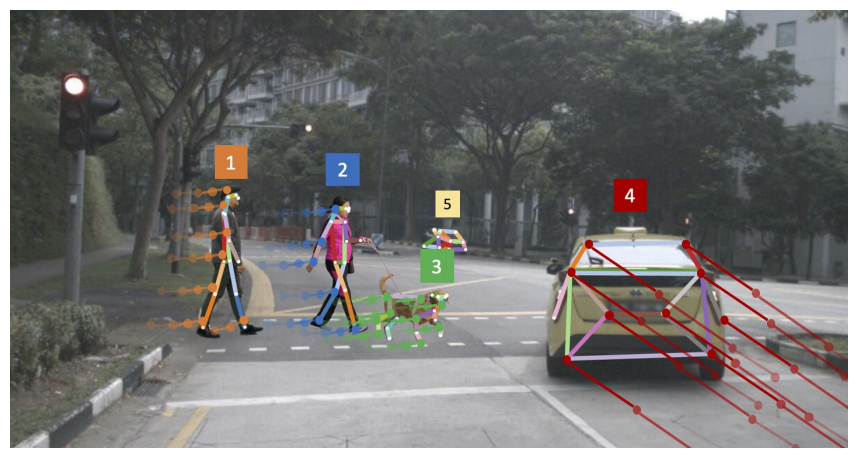
\includegraphics[width=0.4 \textwidth]{Chapters/1. HPE_LUNG/figures/openpifpaf.png}
    \caption{OpenPifPaf: Escena del mundo real desde la perspectiva de un carro autónomo. Todos los
             actores son detectados y seguidos, esto incluye a las personas, el carro y el perro.
             \cite{DBLP:journals/corr/abs-2103-02440}}
    \label{fig:PE-track}
\end{figure}

El problema de \textit{Estimación de Pose Humanos} consiste en predecir las partes del cuerpo o las
posiciones de las articulaciones de una persona a través de una imagen, video. Este problema ha sido
cuidadosamente estudiado a lo largo de los años y diversas recopilaciones de investigaciones han sido escritas.
En la tabla \ref{Tab:hpe-survey} se resumen algunas de las más recientes y que describen dos formas
generales de abordar el problema. La primera de ellas la \quotes{Tradicionalista}, cuyos métodos
usan enfoques clásicos de visión por computadora o la segunda basada en técnicas de aprendizaje
profundo que involucran comúnmente modelos convolucionales. El trabajo realizado en esta tesis está
basado en el segundo método, usando técnicas de aprendizaje profundo y modelos actuales capaces
de capturar información temporal, específicamente enfocado en modelos \textit{Transformers} \cite{Vaswani}.

\begin{table}[ht!]
    \begin{center}
    \resizebox{\textwidth}{!}{%
    \begin{tabular}{|l|l|l|l|}
        % \hline
        % \multicolumn{4}{|c|}{Recopilaciones} \\
        \hline
        \multirow{2}*{\textbf{Título}} & \multirow{2}*{\textbf{Año}} & \textbf{Métodos} & \multirow{2}*{\textbf{Descripción}}\\
         & & \textbf{cubiertos} & \\
        \hline
        \multirow{2}*{A survey of computer vision-based motion capture \cite{MOESLUND2001231}} & \multirow{2}*{2001} & \multirow{2}*{Tradicionales} &  Investigacion general sobre métodos de captura de movimientos basados en visión en\\
        & & & humanos. Incluye estimación de pose, seguimiento y reconocimiento de acciones. \\\hline

        A survey of advances in vision-based human motion capture and analysis \cite{MOESLUND200690} & 2006 & Tradicionales & Incluye una revisión de los métodos de captura de movimiento del año 2001 al 2006.\\ \hline

        \multirow{2}*{Vision-based human motion analysis: An overview. \cite{POPPE20074}} & \multirow{2}*{2007} & \multirow{2}*{Tradicionales} & Investigacion general sobre métodos de captura de movimientos usando datos \\
        & & & sin marcadores de dispositivos de captura. \\\hline

        \multirow{2}*{Advances in view-invariant human motion analysis: A review \cite{5191035}} & \multirow{2}*{2010} & \multirow{2}*{Tradicionales} & Estudio de métodos de estimación de pose en 3D, comportamiento y \\
        & & & reconocimiento/representación de acciones. \\ \hline

        Human pose estimation and activity recognition from multi-view videos: & \multirow{2}*{2012} & \multirow{2}*{Tradicionales} & Métodos de estimación de pose 3D y reconocimiento de acción usando datos \\
        Comparative explorations of recent developments \cite{6193117} &  &  & multi-vista\\ \hline

        A survey of human pose estimation: the body parts parsing based methods \cite{LIU201510} & 2015 & Tradicionales & Estudios de estimación de pose enfocados principalmente a las técnicas de localización \\
        & & & de las distintas partes del cuerpo. \\ \hline

        \multirow{2}*{Human pose estimation from monocular images: A comprehensive survey \cite{Gong2016}} & \multirow{2}*{2016} & \multirow{2}*{Ambos} & Enfocado en la estimación de pose usando datos monoculares incluyendo las\\
        & & & metodologías usadas en procesos tradicionales y basados en aprendizaje profundo. \\ \hline

        \multirow{2}*{3D human pose estimation: A review of the literature and analysis of covariates \cite{SARAFIANOS20161}} & \multirow{2}*{2016} & \multirow{2}*{Deep-Learning} & Revisión general del estado del arte de estimación de pose 3D usando imágenes\\
        & & & y videos RGB. \\ \hline

        \multirow{2}*{Monocular human pose estimation: a survey of deep learning-based methods \cite{CHEN2020102897}} & \multirow{2}*{2020} & \multirow{2}*{Deep-Learning} & Revisión y clasificación general de los métodos de estimación de pose basados en \\
        & & & aprendizaje profundo desde el 2014 usando solo datos monoculares.\\ \hline

        The progress of human pose estimation: a survey and taxonomy \cite{9144178} & \multirow{2}*{2020} & \multirow{2}*{Deep-Learning} & Revisión de los métodos basados en aprendizaje profundo para estimación de \\
        of models applied in 2D human pose estimation &  & & pose 2D\\ \hline

        Deep Learning-Based Human Pose Estimation: A Survey \cite{DBLP:journals/corr/abs-2012-13392} & 2020 & Deep-Learning & Estudio general del estado del arte de estimación de pose 2D y 3D.\\ \hline
    \end{tabular}}
    \end{center}
    \caption{Listado de diversas investigaciones de \textit{Estimación de Pose en Humanos} que abarcan
             tanto enfoques tradicionales como basados en aprendizaje profundo.
             Tabla basada en el trabajo de \citeauthor{DBLP:journals/corr/abs-2012-13392}.}
    \label{Tab:hpe-survey}
\end{table}

\subsection{Taxonomía de Estimación de Pose 2D y 3D}

\begin{figure}\begin{center}
\begin{tikzpicture}[node distance=1.5cm,
        every node/.style={fill=white, font=\sffamily, scale=0.7}, align=center,
        >={Latex[width=2mm,length=2mm]},
        % Specifications for style of nodes:
        % base/.style = {rectangle, rounded corners, draw=black,
        %                 minimum width=4cm, minimum height=1cm,
        %                 text centered, font=\sffamily},
        % activityStarts/.style = {base, fill=blue!30},
        % startStop/.style = {base, fill=red!30},
        % activityRuns/.style = {base, fill=green!30},
        % process/.style = {base, minimum width=2.5cm, fill=blue!10, font=\ttfamily}
        ]
    % Specification of nodes (position, etc.)
    \node (HPE)          []              {HPE};
    \node (2D HPE)       [below of=HPE, left=7.5em of HPE]          {2D HPE};
    \node (3D HPE)       [below of=HPE, right=7.5em of HPE]   {3D HPE \\ Mono/Multi-view};

    \node (2D Single)    [below of= 2D HPE, left=1.0em of 2D HPE]          {2D Single};
    \node (2D Multiple)  [below of= 2D HPE, right=1.0em of 2D HPE]   {2D Multiple};

    \node (3D Single)    [below of= 3D HPE, left=1.0em of 3D HPE]          {3D Single};
    \node (3D Multiple)  [below of= 3D HPE, right=1.0em of 3D HPE]   {3D Multiple};

    \node (2D-Regresion) [below of= 2D Single, left=-1.5em of 2D Single]   {Regresion};
    \node (2D BPD)       [below of= 2D Single, right=-1.5em of 2D Single]   {Body Part \\ Detection};

    \node (2D-TD)        [below of= 2D Multiple, left=-1.5em of 2D Multiple]   {Top-Down};
    \node (2D-BU)        [below of= 2D Multiple, right=-1.5em of 2D Multiple]   {Bottom-Up};

    \node (3D-MF)        [below of= 3D Single, left=-1.5em of 3D Single]   {Model-Free};
    \node (3D-MB)        [below of= 3D Single, right=-1.5em of 3D Single]   {Model-Based};

    \node (3D-TD)        [below of= 3D Multiple, left=-1.5em of 3D Multiple]   {Top-Down};
    \node (3D-BU)        [below of= 3D Multiple, right=-1.5em of 3D Multiple]   {Bottom-Up};

    % Specification of lines between nodes specified above
    % with additional nodes for description
    \draw[-]             (HPE) -- (2D HPE);
    \draw[-]             (HPE) -- (3D HPE);
    \draw[-]             (2D HPE) -- (2D Single);
    \draw[-]             (2D HPE) -- (2D Multiple);
    \draw[-]             (3D HPE) -- (3D Single);
    \draw[-]             (3D HPE) -- (3D Multiple);
    \draw[-]             (2D Single) -- (2D-Regresion);
    \draw[-]             (2D Single) -- (2D BPD);
    \draw[-]             (2D Multiple) -- (2D-TD);
    \draw[-]             (2D Multiple) -- (2D-BU);
    \draw[-]             (3D Single) -- (3D-MF);
    \draw[-]             (3D Single) -- (3D-MB);
    \draw[-]             (3D Multiple) -- (3D-TD);
    \draw[-]             (3D Multiple) -- (3D-BU);

\end{tikzpicture}
\caption{M1 caption for diagram} \label{fig:HPE-diagram}
\end{center} \end{figure}

\subsubsection{Estimación de Pose en 2 y 3 dimensiones}

Existen dos grandes grupos que dividen las metodologías seguidas para la \textit{Estimación de Pose en
Humanos}; estimación de pose en 2 y 3 dimensiones. Cómo el nombre lo sugiere, la \textit{Estimación
de Pose 2D} (\textbf{2D HPE} por sus siglas en inglés) consiste en localizar articulaciones o partes del cuerpo
directamente en imágenes, por tanto, el marco de referencia de las posiciones de cada articulación es la
propia imagen. En la \textit{Estimación de Pose 3D} (\textbf{3D HPE}) las elementos detectados pasan a estar en 3D
y se busca un marco de referencia que mejor se ajuste las dimensiones espaciales de las
articulaciones y personas. Comúnmente se usa un cubo unitario cuyo centro corresponde a la
articulación que indica la cadera o \textit{hip} como se encuentra en la literatura, véase la figura
\ref{fig:HPE-diagram}.

Por otro lado, en muchos escenarios las imágenes contienen más de una persona o se necesita hacer seguimiento
de multiples individuos. Por lo regular cuando aparecen más de un persona en una imagen
(\textbf{MPPE}, Multiple Person Pose Estimation)
se opta por identificar cada cuerpo en la imagen y posteriormente resolver individualmente
la estimación de pose para cada una de las entidades identificadas (\textbf{SPPE}, Single Pose Estimation).
La detección de los cuerpos se realiza en
etapas previas usando modelos de detección de objetos y entrenados para detectar cuerpos
humanos tales como \textit{MobileNet} \cite{DBLP:journals/corr/RenHG015}
\cite{DBLP:journals/corr/HowardZCKWWAA17} \cite{DBLP:journals/corr/abs-1801-04381} o \textit{YOLO}
(You Only Look Once) \cite{DBLP:journals/corr/RedmonDGF15} \cite{DBLP:journals/corr/abs-2004-10934}.

Además, el proceso de estimación de pose puede ser realizado en multiples etapas. Es decir, un modelo
end-to-end puede realizar la tarea completamente o en caso contrario, dividir la tarea en multiples
etapas y usar modelos especializados para resolver cada etapa. Por ejemplo en estimación de pose 3D
es común predecir la pose 2 dimensiones usando una red entrenada para esta tarea y posteriormente
pasar a 3 dimensiones usando la información previa \cite{DBLP:journals/corr/MartinezHRL17}.

\subsubsection{Estimación de Pose 2D Single}

Para la estimación de pose en 2D dónde solo es involucrada una sola personas se usan dos enfoques,
los métodos basado en regresión (\textit{Regresion-Based}) y los métodos basados en detección de
partes del cuerpo humano ((\textit{Detection-Based o Body Part Detection})). Los métodos basados en
regresión estiman las posiciones relacionando directamente la imagen con las coordenadas de las
articulaciones del modelo de cuerpo humano usado. En cambio, los métodos basados de detección
identifican primeramente las partes del cuerpo ya sea a través de marcas como recuadros de las
posiciones o usando mapas de calor que indican las posiciones de las articulaciones.

\subsubsection{Estimación de Pose 3D Single}

Existen dos métodos generales para la estimación de pose 3D en una sola personas, los
\textit{Generativos} y los \textit{Discriminativos}. Los métodos Generativos
también conocidos como (\textit{model-based}, basado en modelos) usan alguna representación de modelos
del cuerpo humano en conjunto con información apriori como los movimientos y el contexto en el que se
ejecutan. Las poses son predecidas usando la imágen un conjunto de representaciones obtenidos de establecer un
función de probabilidad usando información tal como descriptores de la imagen, la estructura del cuerpo
humano, los parámetros de las cámaras y y un conjunto de restricciones derivadas del contexto. Los
modelos Discriminativos simplemente aprenden a predecir directamente la pose usando la datos de entrada
sin usar información de modelos humanos.

\subsubsection{Estimación de Pose 2D-3D Multiple}

% Mono  https://sci-hub.se/10.1109/access.2020.3010248 26-30
% Multi https://sci-hub.se/10.1109/access.2020.3010248 31-35

Bottom-Up: En este enfoque se inicia localizando entidades semánticas y luego agrupandolas
para formar una persona \cite{DBLP:journals/corr/abs-1804-06208} \cite{8578840}
\cite{DBLP:journals/corr/InsafutdinovPAA16}.
Claramente, usando este procedimiento el problema de rendimiento de usar un
estimador de pose por cada persona desaparece, pues todas las entidades de los cuerpos son detectados
a la vez y posteriormente agrupados para formar cada persona, véase la figura \ref{fig:Openpose}.
Sin embargo, el modelo generado tiende
a presentar problemas cuando existen personas ocluyéndose unas a otras. Uno de los trabajos
más conocidos que siguen este marco es OpenPose \cite{8765346}, el cual se ha convertido en una
completa herramienta de referencia para la estimación de pose logrando realizar tareas como
seguimiento en tiempo real y detección de articulaciones en 3D en formato single-person con
opción de triangularizar desde distintas vistas de cámaras, también es posible detectar en tiempo
real la pose en 2 dimensiones tanto el cuerpo humano como gestos con manos y rostros.

\begin{figure}[ht!]
    \centering
    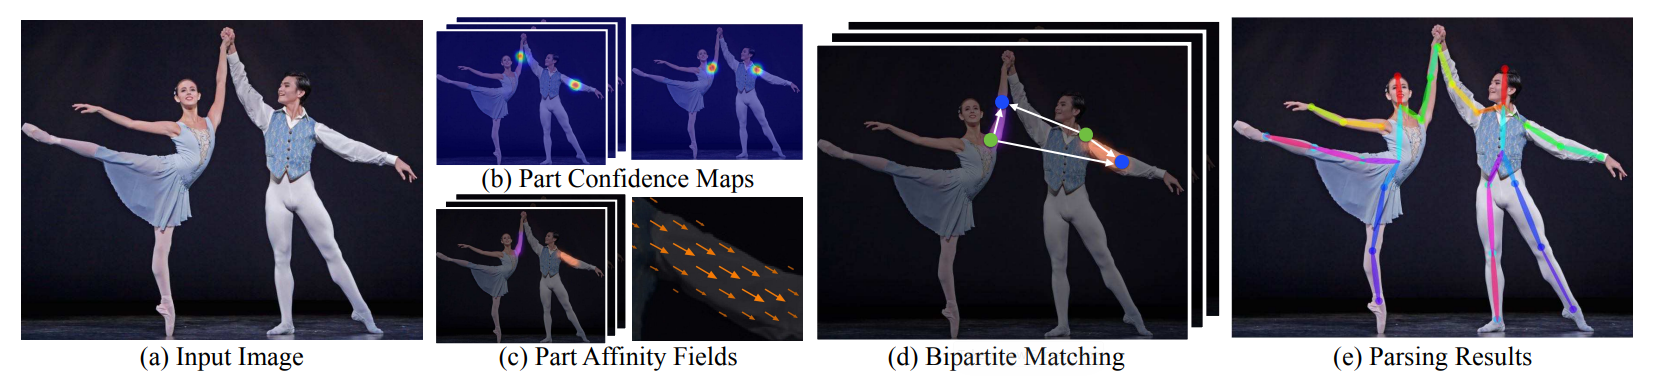
\includegraphics[width=0.8 \textwidth]{Chapters/1. HPE_LUNG/figures/openpose.png}
    \caption{OpenPose: Trabaja bajo un marco Bottom-Pp. Primero predice los mapas de confianza para
             cada parte del cuerpo $b)$ y codifican la orientación y ubicación de las extremidades
             a través $b)$ y $c)$ y finalmente asocian cada miembro identificado y reconstruyen la
             pose del cuerpo $d)$ y $e)$ \cite{8765346}.}
    \label{fig:Openpose}
\end{figure}

Top-Down: El procesamiento se realiza primero detectando los personas individualmente en la imagen
usando un bounding-box proporcionado por algun detector de objetos
\cite{DBLP:journals/corr/NewellYD16} \cite{DBLP:journals/corr/WeiRKS16},
véase la figura \ref{fig:alphapose}.
El principal problema de este enfoque es que si la detección de la persona falla ya no hay nada más
que hacer, y el costo computacional depende de la cantidad de personas en la imagen, puesto que para
cada persona detectada es necesario correr un estimador de pose entrenado para detectar una sola
persona. En contraparte a Openpose, Alpha-Pose \cite{DBLP:journals/corr/FangXL16} sigue el un marco
top-down a través de 3 componentes esenciales; \textit{Symmetric Spatial Transformer Network} (SSTN),
\textit{Parametric Pose Non-Maximum-Suppression}(NMS) y \textit{Pose-Guided Proposals Generator}
(PGPG) que les permiten minimizar el problema de la detección incorrecta o redundante de
bounding-boxes de las personas.

\begin{figure}[ht!]
    \centering
    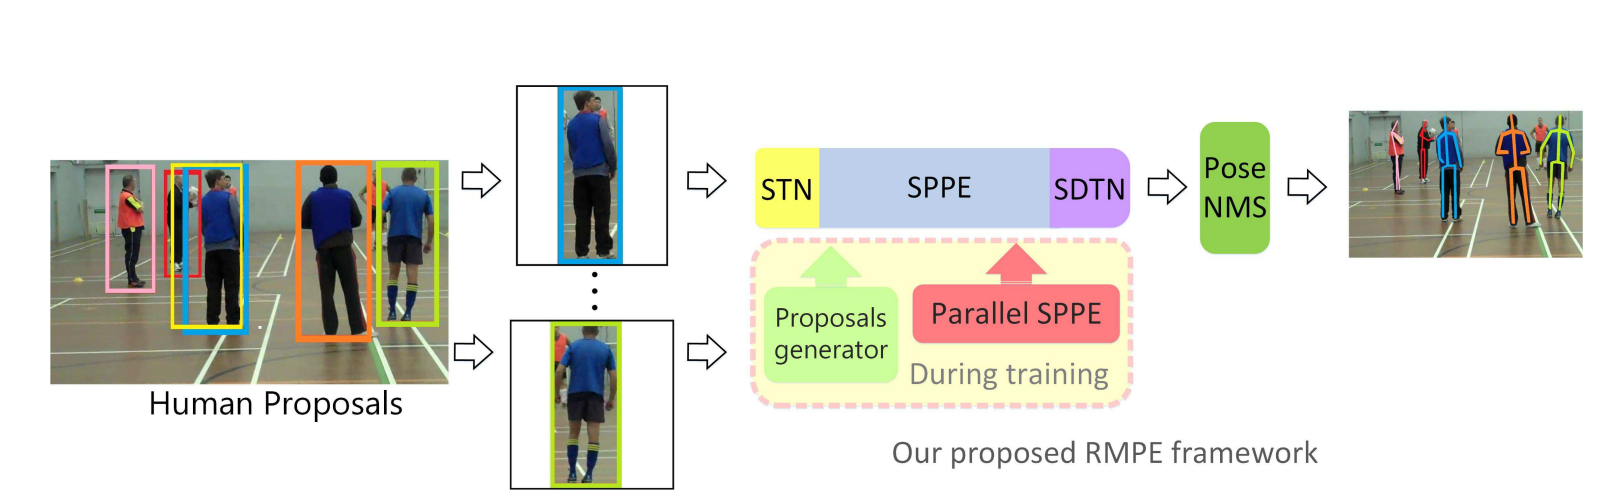
\includegraphics[width=0.8 \textwidth]{Chapters/1. HPE_LUNG/figures/alpha-pose.png}
    \caption{AlphaPose (RMPE): Trabaja bajo un marco Up-Down. Consiste en 3 principales componentes;
            El primero, \textit{Symmetric Spatial Transformer Network} (SSTN) recibe los imágenes de
            las poses a procesar y genera propuestas de poses el
            \textit{Parametric Pose Non-Maximum-Suppression}(NMS) se encarga de eliminar las
            redundancias e inconsistencias y finalmente el \textit{Pose-Guided Proposals Generator}
            (PGPG) es usado como un modelo de aumentación de datos
            \cite{DBLP:journals/corr/FangXL16}.}
    \label{fig:alphapose}
\end{figure}

La estimación de pose en 3d también puede ser realizado en dos marcos, \textit{monocular}
cuando solo se tiene una imagen de reference del sujeto de prueba en un tiempo y pose exacta
\cite{DBLP:journals/corr/MartinezHRL17} \cite{8954163} \cite{DBLP:journals/corr/abs-2002-10322}
\cite{DBLP:journals/corr/abs-1711-08585} \cite{DBLP:journals/corr/abs-2004-11822}
y multi-vista cuando se tienen imágenes desde diferentes perspectivas del sujeto de prueba en misma
la pose y tiempo exacto \cite{DBLP:journals/corr/abs-1905-05754} \cite{DBLP:journals/corr/abs-1901-04111}
\cite{DBLP:journals/corr/abs-2004-06239}.
La ventaja de usar técnicas que puedan aprovechar la información contenida
en diferentes perspectivas es que ayuda a reducir en gran medida la ambigüedad ocasionada por las
oclusiones, una parte puede no ser visible desde un ángulo pero desde otro si. Sin embargo, la
cantidad de conjunto de datos existentes para estimación de pose multi-vista es reducida.


\subsection{Modelado del Cuerpo Humano}

En la solución de los problemas de Estimación de Pose se plantea una arquitectura base para el
cuerpo humano a partir de la cual se adecuarán las estimaciones. Los modelos usados para la
representación del cuerpo humano son 3: \textit{kinematic model}, \textit{Planar Model} y
\textit{Volumetric Model}. véase la figura

\begin{figure}[ht!]
    \centering
    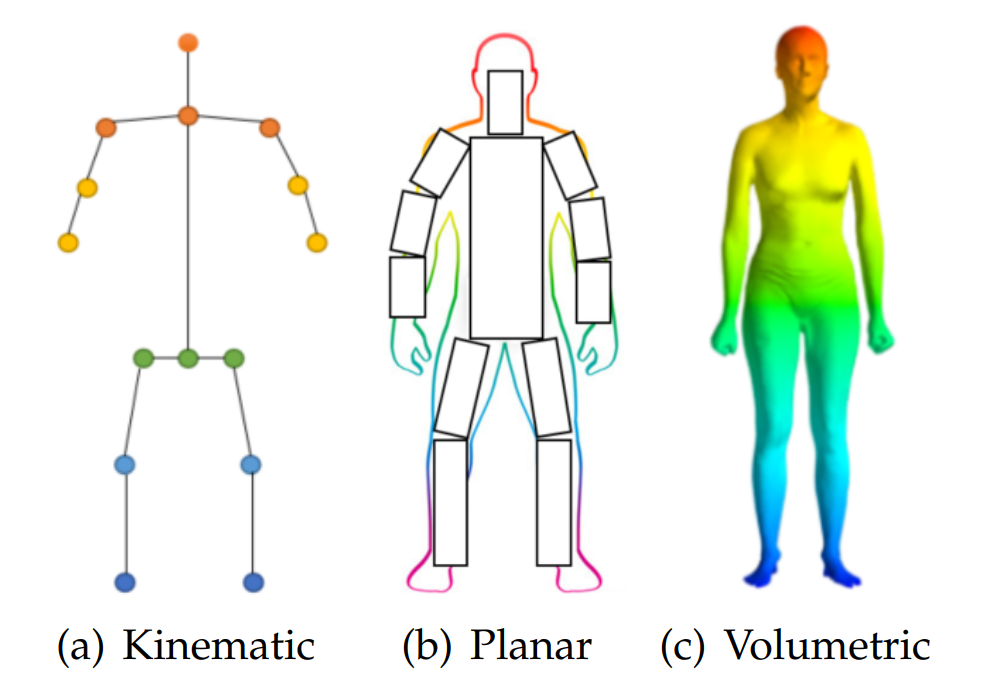
\includegraphics[width=0.7 \textwidth]{Chapters/1. HPE_LUNG/figures/body_model.png}
    \caption{Representaciones de la arquitectura del cuerpo humano. Imagen obtenida de \citeauthor{DBLP:journals/corr/FangXL16}}
    \label{fig:human_rep}
\end{figure}


Skeleton base model, stick figure o kinematic model:
Es uno de los modelos más simples y mayormente usados. Consiste en grafo de nodos que representan
las articulaciones del cuerpo humano, comúnmente entre 10 y 30 nodos \cite{Felzenszwalb2005}.
Así, un hueso es representado como una conexión entre dos articulaciones. Al ser solo una
representación de la estructura del cuerpo carece de demás información como texturas o formas.

Contour-base model o Planar Model:
Es uno de los primeros modelos usados para problemas de Estimación de Pose. Los miembros y torso del
cuerpo humano son representados como un conjunto de rectángulos que proveen información tanto de los
límites de cada miembros como sus longitudes y anchor \cite{557241} \cite{COOTES199538}.

Volumen base model:
Es usado para representar el cuerpo humano y su volumen, es decir es una representación 3D del
cuerpo conseguida a través de un mallado de figuras geométricas y capturados por escaner 3D
\cite{840661}.

\subsection{Tipos de datos}

En los últimos años, debido a la masificación
de dispositivos inteligentes, el acceso a una cámara digital no resulta un problema mayor para la muchas
de las personas, así, la mayoría de los trabajos realizados sobre Estimación de Pose usan
\textit{Imágenes RGB} gracias a su fácil captura y acceso.
Sin embargo, esto solo es cierto en el contexto de la Estimación de Pose 2D, puesto que el etiquetado de datos
usando las coordenadas de la imagen como referencia no representa demasiado problema. En la
Estimación de Pose 3D, la complejidad de la obtención de los datos se incrementa. Para llevar a cabo
el proceso de obtención de los datos es necesario usar equipo especializado y costoso para la captura
de movimiento en acompañamiento de las cámaras de video \cite{6682899}. Hay dos mecanismos de captura
de movimiento, los ópticos y los no ópticos. Generalmente, en los primeros el sujeto de prueba no
necesita de aditamentos complejos como el uso de trajes
(exoesqueleto) y solo un software con ayuda de cámaras, sensores y marcadores se
encargan de registrar e interpretar el movimiento a un modelo digital. Si bien
aventajan en una reducción de coste su precisión es menor que los no ópticos.
El \textit{Kinect}, fabricado por \textit{Microsoft} es uno de los dispositivos más usados
para generar imágenes de infrarrojos (\textit{IR-image}) siendo de fácil encontrarlo y adquirirlo
gracias a su bajo conste. \cite{6165146} \cite{Izadi11kinectfusion:real-time}.

Por otra parte, existen dispositivos basados en tecnologías como \textit{LIDAR} cuya función es
generar imágenes de profundad. Al igual que el \textit{Kinect}, cada vez son de más fácil acceso
debido a su comercialización en dispositivos inteligentes en el último año por compañías como Apple
\cite{DBLP:journals/corr/abs-1711-06396}. El segundo tipo se puede dividir en dos clases;
los mecánicos los cuales usan giroscopios y acelerómetros para registrar el
movimiento y los electromagnéticos, cuyo funcionamiento es a través de la generación un campo
electromagnético y para posteriormente capturar las alteraciones en este que realiza el sujeto al
moverse \cite{articleMotion}.

\subsubsection{Conjuntos de Datos más usados para estimación de pose 2D y 3D}

\textbf{MPII Human Pose Dataset}: Es un dataset para estimación de pose en modalidades de
single-person o multi-person en 2 dimensiones \cite{andriluka14cvpr}. Incluye al rededor de 25 mil
imágenes conteniendo
40 mil de ellas de personas con anotaciones de las articulaciones del cuerpo realizando diversas
actividades. En total se agrupan en en 410 actividades recolectadas de videos de \textit{YouTube}.

\textbf{Microsoft COCO Dataset}: Es un dataset publicado por \textit{Microsoft} para tareas de
detección de objetos, segmentación y subtitulado de imágenes (image captioning), su última version
disponible corresponde a la del año 2017 \cite{DBLP:journals/corr/LinMBHPRDZ14}. Contiene al rededor
de 80 categorías de imágenes y de estas 66,808 mil son de personas con un aproximado de 250 mil
con total de aproximado de 273,469 anotaciones de cuerpos humanos. Sin embargo, No todas las
imágenes contienen anotaciones de las 17 articulaciones, por lo que los modelos tienen que predecir
cuales y cuántas articulaciones están presentes. Ambas modalidades single-person y multi-person en 2
dimensiones están disponibles en las imágenes.

% DensePose
% Number of images: 50K
% Number of annotated correspondences: 5M
% Year: 2018
% DensePose is a large-scale ground-truth dataset with image-to-surface correspondences manually
% annotated on 50K COCO images. To build this dataset Facebook AI Research team involved human
% annotators, who were establishing dense correspondences from 2D images to surface-based
% representations of the human body using a specifically developed annotation pipeline.


\textbf{HumanEva Dataset}: Dataset usado para estimación de pose en 3 dimensiones en modalidad de
single-person. Contiene diversos secuencias de videos grabadas con cámaras en formato RGB y escala
de grises. Está compuesto de dos sub-datasets \textit{HumanEva I} y \textit{HumanEva II} la principal
diferencia es el sistema de captura, el primero fue a través de software marcadores con 6 cámaras
y el segundo a través de hardware con 8 cámaras, ambos dentro de un ambiente controlado.

\textbf{Human3.6M Dataset}: Contiene aproximadamente 3.6 millones de imágenes de poses humanas
correspondientes a la cantidad de frames de secuencias de videos sobre 11 diferentes actores, 6
hombres y 3 mujeres realizando
17 distintas actividades \cite{6682899}. Cada video fue realizado a usando un total de 10 cámaras de
motion capture en un ambiente controlado interno.

\textbf{TotalCapture Dataset}: Similar a Human3.6M, contiene contiene aproximadamente 1.9 millones
de frames en videos en modalidad single-person y multi-vista calibrado a través de 8 cámaras.

\subsubsection{Conjuntos de Datos Sinteticos}

\textbf{SURREAL (Synthetic hUmans foR REAL tasks)} (2017): Es un dataset en modalidad single-person para
estimación de pose 2D y 3D. Los datos originales son tomados del dataset Human3.6M y aleatoreamente
muestreados (pose de la persona, apariencia, luz ambiental, posición de la cámara, tipos de fondos
en las imágenes, texturas, etc.) para crear sintéticamente personas y escenas
\cite{DBLP:journals/corr/Varol0MMBLS17}.

\textbf{JTA Dataset} (2018): Dataset sumamente grande creado a partir de simulaciones de
\textit{Grand Theft Auto V} desarrollado por \textit{Rockstar North} \cite{fabbri2018learning}
para estimación de poses 2D y 3D. Contiene al
rededor de 500 mil frames y 10 millones de poses de poses en escenarios urbanos todos ellos con
anotaciones completas de posiciones en 3D.

A pesar de que los datasets sintéticos son mucho grandes que los otros, actualmente no son tan
aceptados en la comunidad y su uso benchmark como benchmark no es visto principalmente dado que son
datos sinteticos. Sin embargo puesto que en los datos sintéticos se tiene mucho mayor control
del ambiente puede solventar varias de las debilidades de los otros datasets como oclusiones, cambios
de luz, tipos y colores de ropa, distintos contextos de fondos de imagen llevando modelos más robustos
y con mejor generalización. La mayoría de la bases de datos son obtenidas a través de algunos pocos
sujetos de prueba y la estructura fisiológica de individuos no es perfecta. Esta variación es causada
por diversos diversos factores como el sexo, la raza, edad, lugar de nacimiento y desarrollo,
enfermedades, factores genéticos, entre otros, además de que los movimientos recreados entre sujetos
no siempre son hechos de la misma manera aunque las circunstancias o ambiente esté controlado.

Con los datos son obtenidos bajo un ambiente controlado es posible obtener imágenes fieles para el
entrenamiento. Aún así, los modelos al ser desplegados en ambientes reales
se enfrentan a imprevistos de los que no se puede tener control; oclusiones de diversas partes del
cuerpo que no fueron provistas durante el entrenamiento ya sea por el mismo sujeto o algún objeto
extraño en la captura, movimientos extraños o rápidos como correr o dar una patada donde el modelo
no puede los puede identificar o el equipo de captura no pueda obtener que se ven como fotogramas
borrosos.

% Modern pose estimation algorithms are almost exclusively based on convolutional neural networks
% with hourglass architecture or its variants (see the image below). Such a network consists of two
% major parts: a convolutional encoder that compresses the input image into the so-called latent
% representation and decoder that constructs N heatmaps from the latent representation where N is the
% number of searched keypoints.

\subsubsection{Métricas de Evaluación}

\textbf{Percentage of Correct Parts (PCP)}: Mide la tasa de detección de extremidades. Una extremidad
o parte de un cuerpo es considerada detectada si el promedio de la distancia de las posiciones entre dos
articulaciones predichas y la distancia de las posiciones de las articulaciones de la extremidad real
es menor que cierto umbral \cite{4587468}. El umbral comúnmente tomado corresponde al 50\% de la distancia de la
longitud de la extremidad real en cuestion:

\begin{equation}
    \frac{||c_s^{(n)} - \hat{c}_s^{(n)}|| + ||c_e^{(n)} - \hat{c}_e^{(n)}||}{2} \le \alpha\ || c_s^{(n)} - c_e^{(n)} ||
    \label{eq:PCP}
\end{equation}

$||c_s^{(n)}$ y $||c_e^{(n)}$ representan las coordenadas de las dos articulaciones (inicial y final
respectivamente) de la n-ésima extremidad. $||\hat c_s^{(n)}$ y $||\hat c_e^{(n)}$ son las coordenadas
inicial y final de las dos articulaciones predichas de la n-ésima extremidad. $\alpha$ funciona como
el umbral de error. Actualmente, ya no se usa esta métrica debido a que penaliza mayormente las partes
del cuerpo más pequeñas. Mientras mayor es su \textit{PCP} mejor es el modelo.


\textbf{Percentage of Detected Joints (PDJ)}: Esta métrica fue propuesta para sobrellevar la
limitante antes mencionada de \textit{PCP}. Mide la tasa de detección de articulaciones del cuerpo.
Una articulación es correctamente detectada si la distancia entre la posición de la articulación
detectada y la posición real de la articulación está dentro de cierta fracción del diámetro del torso,
es decir la distancia entre la cadera derecha (right hip) y el hombro izquierdo (left shoulder)
\cite{6619315} \cite{DBLP:journals/corr/ToshevS13}:

\begin{equation}
    ||c^{(i)} - \hat{c}^{(i)}|| \le \alpha\ || c_{rh} - c_{ls} ||
    \label{eq:PDJ}
\end{equation}

$c^{(i)}$ es la coordenada de la i-ésima articulación y $\hat c^{(i)}$ es la coordenada de la
articulación predicha correspondiente. $c_{rh}$ es la coordenada de la cadera derecha y $c_{ls}$
es la coordenada del hombro izquierdo. El problema con esta métrica es que cuando la persona se es
capturada de lado en una imagen 2D el diámetro del torso tiende a ser cero así como la distancia
entre la cadera derecha e izquierda.

\textbf{Percentage of Correct Key-points (PCK)}: Es similar a la métrica \textit{PDJ} pero en vez de
tomar el diámetro del torso se toma la distancia de la diagonal del rectangulo externo que rodea
todas las articulaciones del cuerpo \cite{6380498}.

\begin{equation}
    ||c^{(i)} - \hat{c}^{(i)}|| \le \alpha\ diag_{bbox}
    \label{eq:PCK}
\end{equation}

La ecuación \ref{eq:PCK} correspondiente al cálculo de la detección correcta de articulación para la
métrica de \textit{PCK} es similar a \textit{PDJ}. Una tercer variación es considerando una
proporción de la longitud del segmente de la cabeza como umbral \cite{6909866},
\textit{head-normalized probability of the correct keypoint} o \textit{PCKh}, con la finalidad
de tener un umbral independiente de las distancias de las articulaciones y una posible elección
es usar el tamaño de la cabeza del sujeto a prueba.

\textbf{Average Precision (AP) y Average Recall (AR)}: Inicialmente introducido
como  \textit{Average Precision of Keypoints (APK)} \cite{6380498} mide la exactitud y rendimiento
de la detección de las articulaciones de acuerdo a la proporción de verdaderos positivos sobre el
total de positivos detectados (precision) $\frac{TP}{TP + FP}$ y la proporción
de verdaderos positivos sobre el total de positivos (recall) $\frac{TP}{TP + FN}$ penalizando tanto
detecciones no encontradas como falsas detecciones. Al igual que los anteriores hay variantes
como Mean Average Precision (mAP) que es la media de la precisión del modelo para todas las
clase. Todos basados en alguna medida de similaridad como la propuesta en
\textit{Object Key-points Similarity (OKS)} que mide el promedio de cercania de las articulaciones
predichas y las reales. Definen una similaridad entre articulaciones (Keypoint Similarity)
\cite{DBLP:journals/corr/LinMBHPRDZ14}
como la distancia entre las articulaciones predichas normalizadas por la escala del
área que forma la persona y una constante de regularización determinada para cada articulación:

\begin{equation}
    KS = \exp(- \frac{||c^{(n)} - \hat{c}^{(n)}||^2}{2s^2 k^2_n})
    \label{eq:KS}
\end{equation}

$s$ y $k_n$ corresponden al factor de escala equivalente a la raíz cuadrada del área segmentada del
objeto y a la constante de regularización por cada tipo de articulación cuya su función conjunta
es regular la importancia de cada articulación.


\textbf{Mean Per Joint Position Error (MPJPE)}: Calcula el error en milímetros determinado por la distancia
euclidiana entre los articulaciones predichas y las reales sobre cada tipo de articulación de la
imagen o imágenes en caso de videos. Para distintos datasets de predicción de pose en 3D existen
más de un pre-procesamiento antes calcular el error \textit{MPJPE} conocidos como protocolos.
Por ejemplo para \textit{Human3.6M} el Protocolo \#1 consiste en alinear las coordenadas de las
articulaciones con respecto a la raíz, generalmente la que corresponde al centro de la cadera (hip).
El Protocolo \#2 calcula el error después de realizar un alineamiento mediante una transformación
rígida usando \textit{Procrustes Analysis} \cite{Gower1975}, también abreviado como \textit{P-MPJPE}.

\begin{equation}
    MPJPE = \frac{1}{M} \sum_{i=1}^M ||c^{(i)} - \hat{c}^{(i)}||
    \label{eq:MPJPE}
\end{equation}

$M$ corresponde a el total de articulaciones. Generalmente el error es calculado por tipo, clase o
acción representado en los videos.

Al igual que en estimación de pose 2D la métrica de PCK o 3DPKC es usada para estimación de pose en
3D, al igual que su area bajo la Curva (AUC) considerando típicamente un umbral de 150mm que se
aproxima a la mitad del tamaño de la cabeza \cite{DBLP:journals/corr/MehtaRCSXT16}. Por otro lado,
datasets usados para estimación de pose 3D son basados en secuencias de videos y una variante a
\textit{MPJPE} es introducida \cite{8954163} para considerar la suavidad de las transiciones entre
poses midiendo la velocidad de las articulaciones (en milímetros por segundo),
\textit{Mean Per Join Velocity Error (MPJVE)}, que corresponde al error \textit{MPJPE} primer
derivada de las secuencias de pose 3D.

\textbf{Mean Joint Angle Error (MJAE)}: Es similar al error \textit{MPJPE} pero usando los ángulos de
cada articulación. Mide el error como promedio sobre todos los ángulos de la diferencia absoluta
entre la articulación estimada y la real de acuerdo a su posición angular:

\begin{equation}
    MPJPE = \frac{1}{M} \sum_{i=1}^M |(c^{(i)} - \hat{c}^{(i)}) \mod \pm 180^{\circ}|
    \label{eq:MJAE}
\end{equation}

\section{Detección de Patologías en Pulmones Mediante Imágenes de Rayos-X}

A pesar de diversos esfuerzos para desarrollar métodos basados en aprendizaje máquina basados en
análisis de imágenes de Rayos-X y Tomografías Computarizadas aún no están listos para uso clínico.
Limitaciones como sesgos debido a bases de datos pequeñas o recopilaciones de diversas fuentes sin
un tratamiento o normalización entre estos, así como enfoques de detección en enfermedades
específicas dejando de lado la posible contribución a los modelos la inclusión de otras enfermedades.
Por ello el trabajo presentado en este escrito se concentra en desarrollar un modelo basado en
aprendizaje profundo atacando estás problemas. El modelo desarrollado es entrenado para la detección
de 15 patologías de pulmones, incluyendo \textit{COVID-19}.

El padecimiento por \textit{COVID-19} es una enfermedad contagiosa causada por el \textit{Síndrome
Respiratorio Agudo Severo Coronavirus 2} o \textit{SARS-CoV-2} por sus siglas en inglés
(\textit{Severe Acute Respiratory Syndrome Coronavirus 2}) reportada por primera vez en diciembre
del año 2019 como un nuevo tipo de pneumonia viral \cite{huang2020clinical}. Pocos meses después,
en marzo del 2020 el \textit{COVID-19} fue declarado como pandemia a nivel mundial por la
Organización Mundial de la Salud (\textit{WHO}) \cite{world2020director}. Los métodos más eficaces
de detección de \textit{COVID-19} son la prueba clínica de Reacción en Cadena de Polimerasa con
Transcripción Inversa
(\textit{RT-PCR}) también llamada genéricamente \textit{molecular photocopying test} pues es usada
para amplificar-copiar pequeños
segmente de \textit{DNA} y detectar material genético de un organismo en específico como el virus
\textit{SARS-CoV-2} y mediante la búsqueda de anticuerpos desarrollados por el organismo como
respuesta a la enfermedad con la Prueba Rápida de Anticuerpos (\textit{RAT})
\cite{Gupta2021, Apra2021, pub.1136450856, LIU2021112817}. Puesto que los
anticuerpos tardan en generarse entre los 10 y 20 días después de la infección
\cite{lou2020serology,o2021age,VABRET2020910}, la pruebas tipo \textit{PCR} es preferida como
método de detección temprana. En la ausencia de prueba \textit{PCR}, los pacientes con sintomatología
similar a la provocada por \textit{COVID-19} solo pueden ser diagnosticados con pneumonia atípica
como padecimiento. Por ello, diversos métodos de análisis de imágenes basados en técnicas
de Inteligencia Artificial han sido desarrollados para la detección de \textit{COVID-19} usando
imágenes de Rayos X y Tomografías Computarizadas. Reportes clínicos indican que imagenes de Rayos X
y Tomografías Computarizadas de pecho pueden mostrar efectos de afectaciones por \textit{COVID-19}.
Dichos efectos pueden ser apreciados en los pulmones incluso en casos donde la prueba PCR resulta
en Falso Negativo \cite{ai2020correlation, wong2020frequency}. Así, la principal motivación es
desarrollar métodos alternativos que ayuden a la detección de \textit{COVID-19} dada la limitada
disponibilidad, creciente demanda, costo asociado y la obtención de resultados inmediatos de la
aplicación de técnicas como \textit{PCR} en todo el mundo.

Un práctico y exitoso enfoque en la implementación de Redes Neuronales Profundas (DNNs) de dominio
específico \cite{liu2017survey} basados en técnicas de clasificación es usar Transferencia de
Conocimiento (Deep Transfer Learning, DTL) \cite{long2016unsupervised,oquab2014learning,tan2018survey}.
Esta técnica fue inicialmente desarrollada para implementar modelos de dominio en específico en
situaciones en las que se cuenta con una cantidad de datos limitada, pero también se ha visto que
usar técnicas de DTL resulta en un método efectivo para entrenar modelos de dominio en específico aún
cuando se tiene suficientes datos. Particularmente, en problemas de clasificación, la Transferencia
de Conocimiento consiste en reusar modelos de Aprendizaje Profundo entrenados en problemas de
dominio general en donde los conjuntos de datos son lo suficientemente grandes. Dado que la tarea de
clasificación contiene un gran número de clases y datos, los modelos entrenados pueden generalizar y
extraer mejores características de bajo nivel. Por lo que, el uso de Transferencia de Conocimiento
también ha sido efectivo en el desarrollo de modelos específicos para el análisis de imágenes médicas
\cite{deniz2018transfer,litjens2017survey, sufian2020survey}, tales como la detección de
\textit{COVID-19} a partir de imágenes de Rayos X, problema atacado ampliamente por la comunidad
usando Transferencia de Conocimiento en Modelos basados en Aprendizaje Profundo
\cite{agrawal2021focuscovid,ai2020correlation,sufian2020survey}.

A pesar de los esfuerzos en desarrollar diversos métodos de aprendizaje máquina para la detección de
\textit{COVID-19} basados en Rayos X y Tomografías Computarizadas, los resultados obtenidos y
reportados hasta el momento aún no están listos para uso clínico \cite{roberts2021common}.
\citeauthor*{shuja2021covid} presenta una relación de los conjuntos de datos abiertos de
\textit{COVID-19} categorizándolos por tipo (imágenes biomédicas,
datos textuales y de audio), aplicaciones y métodos aplicados de \textit{IA}, \textit{Big Data} y
estadísticos. Sin embargo, las imagenes en los datasets mencionados son reducidos y limitados a
regiones específicas alrededor del mundo. Por otro lado, \citeauthor{greenspan2020position} mencionan
que la mayoria de los modelos reportados fueron probados en bajo en esquema de diagnóstico bastante
estrecho, puesto que los modelos deberían ser capaces de detectar \textit{COVID-19} en conjunto
con una amplia variedad de patologías. De acuerdo a \citeauthor{roberts2021common} los fallos comunes
son, entre otros, el sesgo en datasets pequeños o datasets no normalizados recolectados de una larga
variedad de fuentes. \citeauthor{roberts2021common} también argumenta la importancia de desarrollar
modelos no solo para la clasificación binaria de \textit{COVID-19}, sino además poder distinguirlo
de otros tipos de neumonías virales y bacteriales. El trabajo descrito a continuación se centra en
atacar el problema en los términos anteriores, no solamente haciendo la distinción entre
\textit{COVID-19} y otros tipos de neumonías sino a través de diversas enfermedades en afán de ayudar
a clínicos en el diagnóstico de otras patologías mas allá de neumonía.

\section{De RNN's a Transformers}

Las \textbf{Redes Neuronales Recurrentes} o \textbf{RNN} (por sus siglas en Inglés) basadas en el
trabajo de \citeauthor{Rumelhart} datan del año 1986. Este tipo de redes están especializadas
en el procesamiento de datos que contienen información temporal, mejorando los resultados obtenidos
por otros tipos de redes como \textit{Redes FeedForward} o \textit{Redes Convolucionales}.

La idea principal detrás de estos modelos de redes es el concepto de \textit{Parameter Sharing}.
Usando \textit{Parameter Sharing} un modelo puede generalizar mejor cuando la información
está contenida en diferentes partes de una secuencia. Así, el modelo no necesita aprender
independientemente todas las reglas que forman la secuencias, sino que ahora, la salida para cada
elemento perteneciente a un tiempo $t$ está determinada por la salida del elemento anterior $t-1$.
Resultando en una recurrencia con las mismas reglas de actualización aplicadas a cada elemento en el tiempo.
La ecuación \ref{eq:rnnh} representa este proceso; $h^{(t)}$ es el estado de la recurrencia definida
por una función $f$ sobre un elemento $x^{(t)}t$ de la secuencia $X$ en el tiempo $t$ y $\theta$ son
los parámetros compartidos.

\begin{equation}
    h^{(t)} = f(x^{(t)}, h^{(t-1)}; \theta)
    \label{eq:rnnh}
\end{equation}

En una \textit{RNN} vista como un \textit{gráfo computacional dirigído y acíclico}, cada nodo
representa un estado en la recurrencia y procesa la información de la secuencia $X$ con los mismos
parámetros $\theta$ en cada paso, observe la figura \ref{fig:rnn_cg}.

\begin{figure}[!ht]
\centering
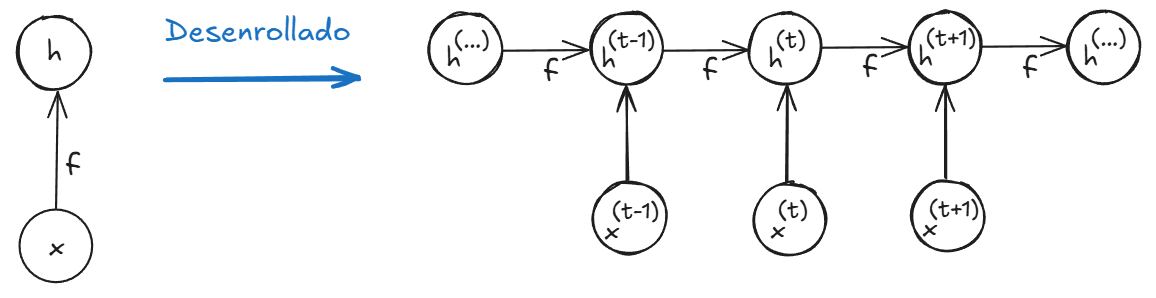
\includegraphics[width=.8\textwidth]{Chapters/2. Transformer/Figures/rnn/rnn_cgraph.png}
\caption[RNN - Grafo Computacional]{Grafo computacional generado por una \textit{RNN} al
        \quotes{desenrollar} la recurrencia. Usando los parámetros compartidos en cada nodo
        y con cada elemento $x^{(t)}$ de la secuencia genera un nuevo estado oculto $h^{(t)}$
        para retroalimentar nuevamente la entrada del siguiente nodo.}
\label{fig:rnn_cg}
\end{figure}

% Redes Neuronales Recurrentes más comunes
\subsection{Redes Neuronales Recurrentes más comunes}

Existen diversas formas como construir \textit{Redes Neuronales Recurrentes}, estas pueden producir una
salida en cada paso de tiempo o tener solo una al final de la recurrencia  o tener
conexiones entre unidades ocultas. La manera más común de implementar una \textit{RNN} está ilustrada en la
figura \ref{fig:rnn_cfga}. En esta figura, cada etapa de la recurrencia es retroalimentada por la
activación del estado oculto previo. Así, $h^{(t)}$ contiene información codificada de elementos
previos de la secuencia que puede ser usada en el futuro para obtener una salida $O^{(t+1)}$. En la
figura \ref{fig:rnn_cfgb} se
cambia la retroalimentación de $h^{(t)}$ por $o^{(t)}$. Nótese que en este caso, la red es entrenada
para obtener un valor en específico $o^{(t)}$ lo que provocaría que gran parte de la información de
los estados ocultos pasados $h^{(t-1)}, h^{(t-2)}, ...$ no se transmita.
La diferencia entre los dos esquemas anteriores es que
la red \ref{fig:rnn_cfga} es entrenada para decidir que información debe transmitir en el futuro a través
de los estados ocultos, en cambio, en la figura \ref{fig:rnn_cfgb} cada estado esta conectado con el
pasado a través de la predicción del paso anterior, perdiendo así gran parte de la información
codificada en cada estado oculto $h^{(t)}$. Este no sería un problema si la salida $O^{(t-1)}$ fuese
lo suficientemente enriquecedora y en altas dimensiones.

% \begin{figure}[!ht]
% \centering
% 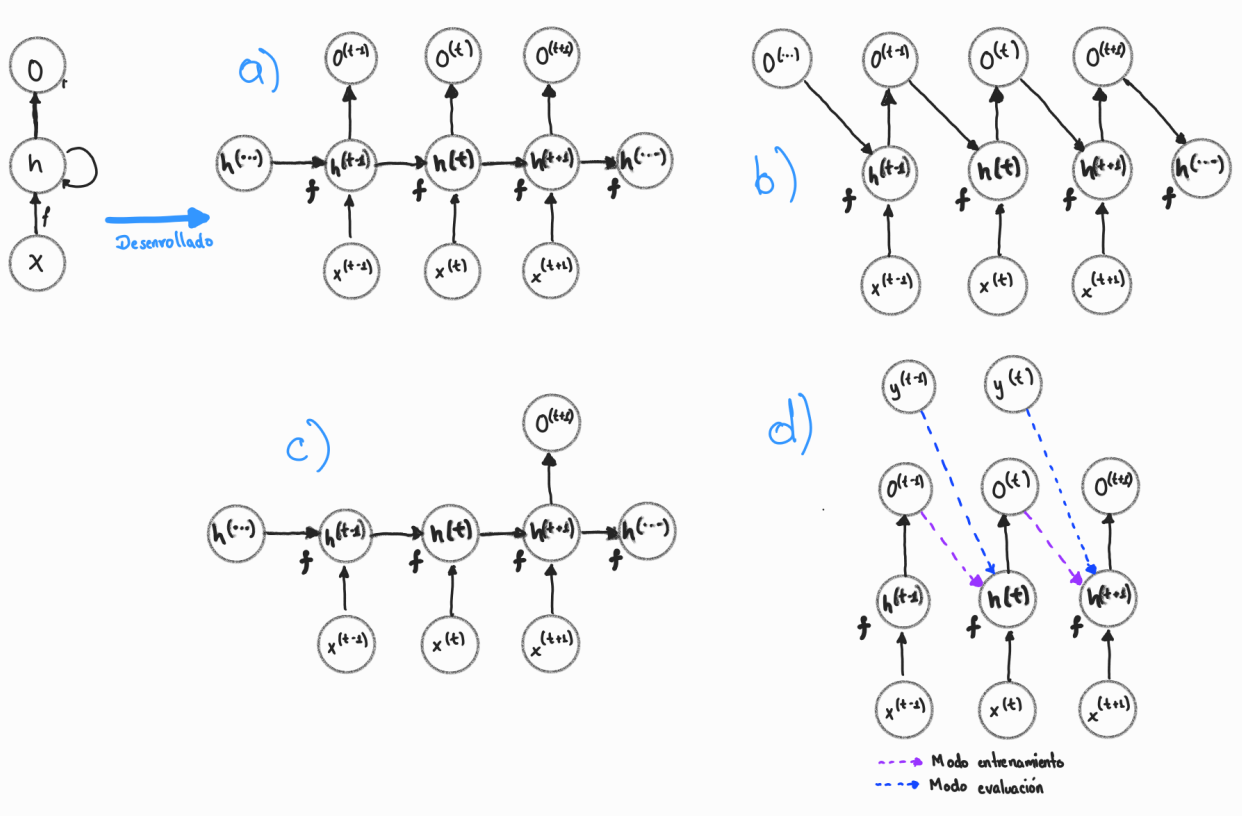
\includegraphics[width=.8\textwidth]{Chapters/2. Transformer/Figures/rnn/rnn_cfg.png}
% \caption[RNN - CFG]{Distintos tipos de RNNs. \textbf{a)} Las activaciones de las capas ocultas $h^{(t)}$
% alimentan al nodo siguiente, cada etapa de la recurrencia genera una salida $o^{(t)}$ \textbf{b)}
% Cada nodo es alimentado por las salidas de cada estado oculto $o^{(t)}$. \textbf{c)} Al final de la
% recurrencia solo tiene una salida $o^{(T)}$, puede ser usada para resumir/predecir un valor de una
% secuencia. \textbf{d)} Teacher Forcing. En modo de entrenamiento cada nodo en el tiempo $t$ es
% retroalimentado por la salida correcta $y^{(t-1)}$, en modo evaluación es retroalimentado por las
% salidas del modelo $O^{(t-1)}$}
% \label{fig:rnn_cfg}
% \end{figure}

\begin{figure}[!ht]
    \centering
    \begin{subfigure}[b]{0.49\textwidth}
        \centering
        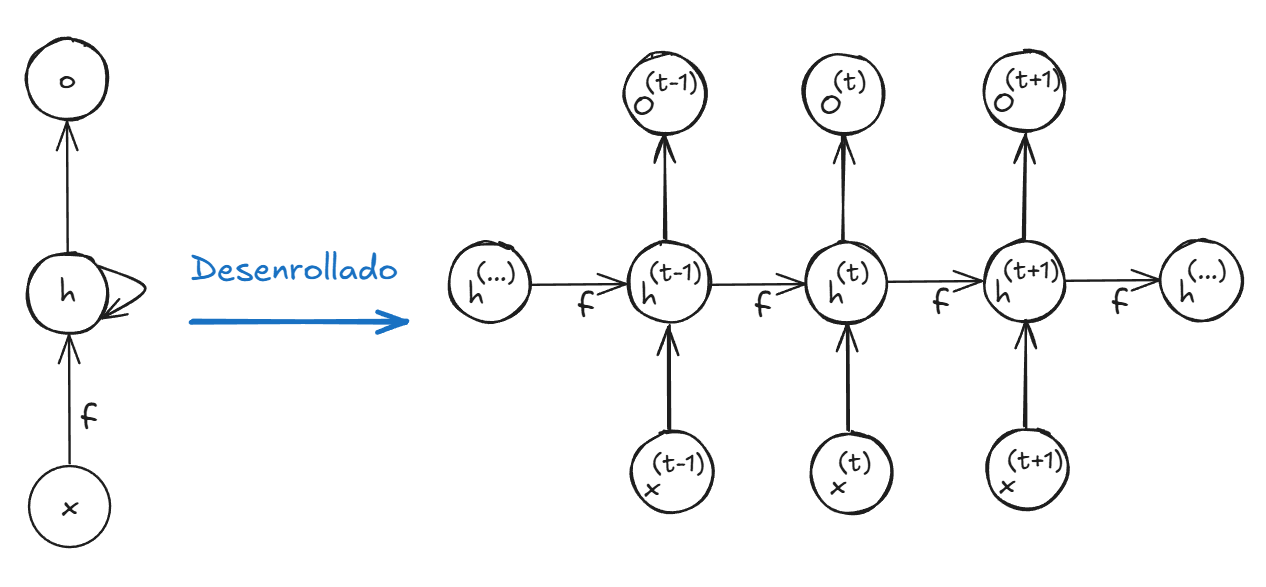
\includegraphics[width=\textwidth]{Chapters/2. Transformer/Figures/rnn/rnn_cfga.png}
        \caption{Las activaciones de las capas ocultas $h^{(t)}$
        alimentan al nodo siguiente, cada etapa de la recurrencia genera una salida $o^{(t)}$.}
        \label{fig:rnn_cfga}
    \end{subfigure}
    \hfill
    \begin{subfigure}[b]{0.4\textwidth}
        \centering
        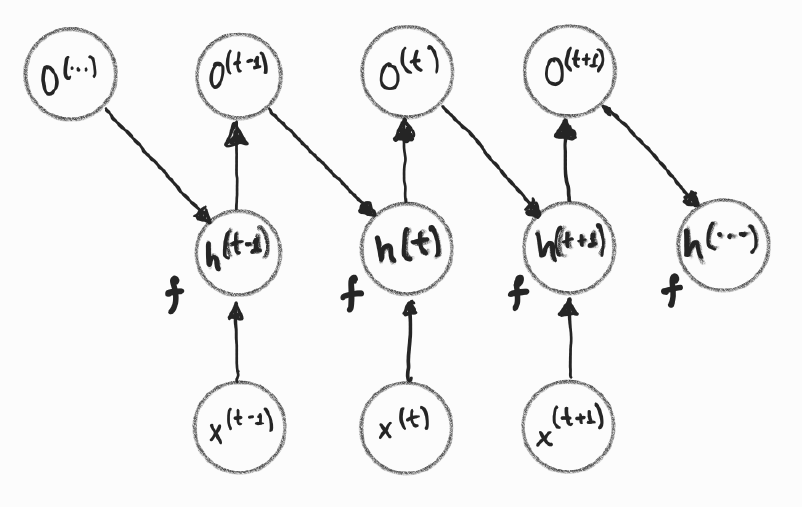
\includegraphics[width=\textwidth]{Chapters/2. Transformer/Figures/rnn/rnn_cfgb.png}
        \caption{Cada nodo es alimentado por las salidas de cada estado oculto $o^{(t)}$.}
        \label{fig:rnn_cfgb}
    \end{subfigure}

    \begin{subfigure}[b]{0.4\textwidth}
        \centering
        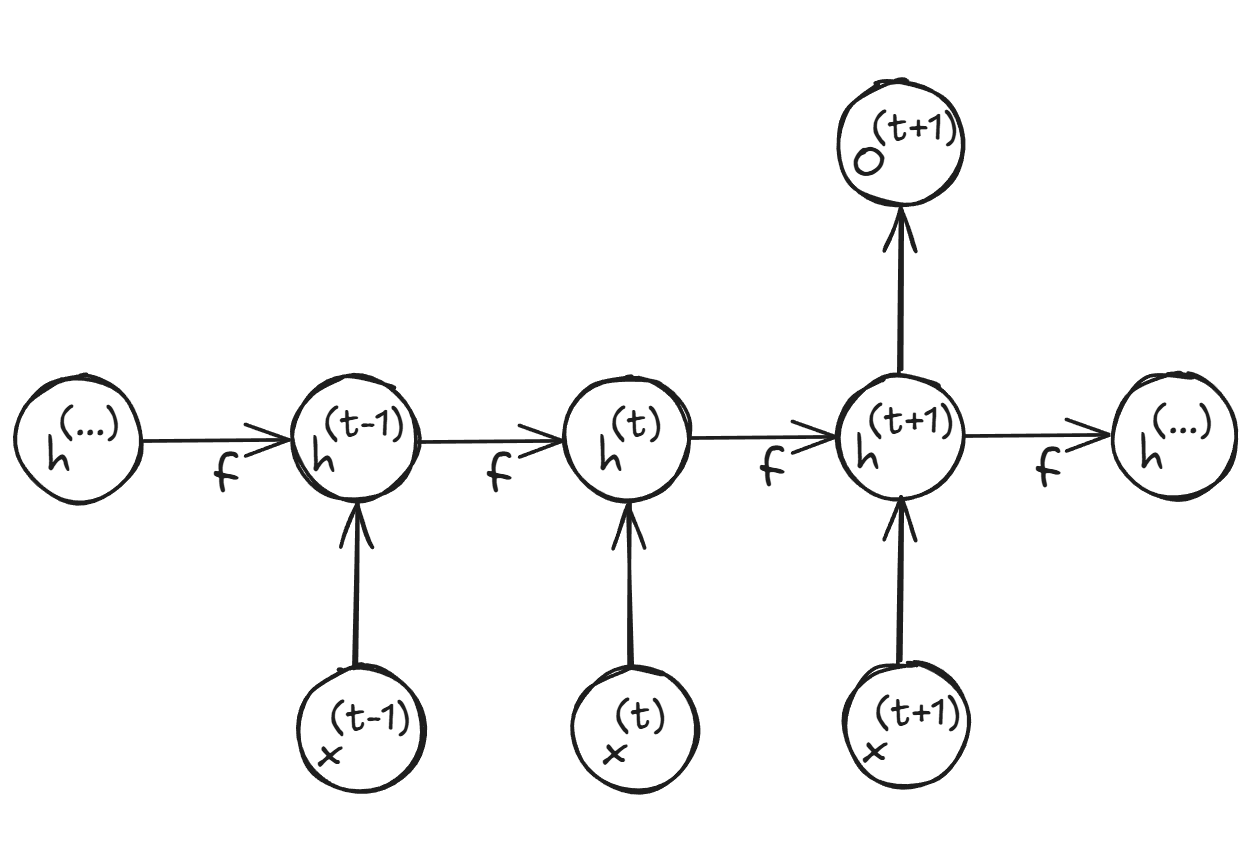
\includegraphics[height=0.63\textwidth]{Chapters/2. Transformer/Figures/rnn/rnn_cfgc.png}
        \caption{Al final de la recurrencia solo tiene una salida $o^{(T)}$, puede ser usada para
        resumir/predecir un valor de una secuencia.}
        \label{fig:rnn_cfgc}
    \end{subfigure}
    \hfill
    \begin{subfigure}[b]{0.49\textwidth}
        \centering
        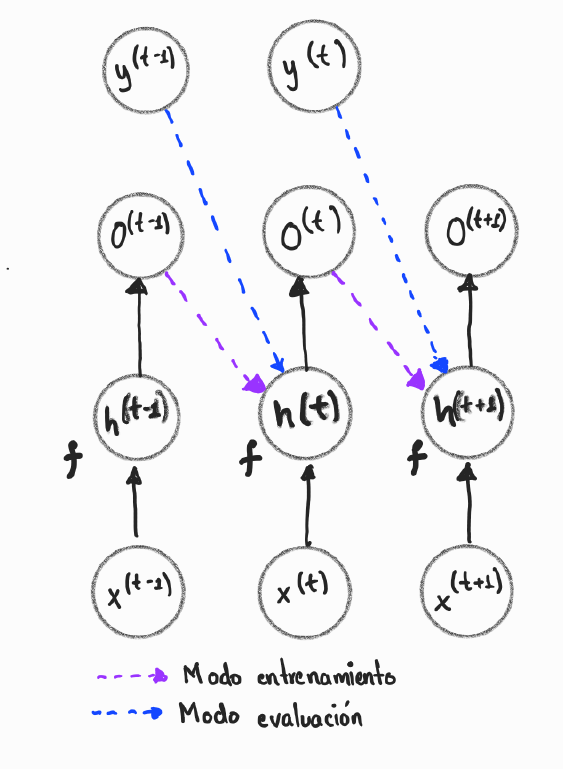
\includegraphics[height=0.6\textwidth]{Chapters/2. Transformer/Figures/rnn/rnn_cfgd.png}
        \caption{Teacher Forcing. En modo de entrenamiento cada nodo en el tiempo $t$ es
        retroalimentado por la salida correcta $y^{(t-1)}$, en modo evaluación es retroalimentado por las
        salidas del modelo $O^{(t-1)}$.}
        \label{fig:rnn_cfgd}
    \end{subfigure}

    \caption[RNN - CFG]{Distintos tipos de RNNs.}
    \label{fig:three graphs}
\end{figure}


Por otro lado, la \textit{RNN} representada en la figura \ref{fig:rnn_cfgc} tiene una sola salida al
final de la recurrencia.
Al contrario de las anteriores, este tipo de redes pueden ser usadas para resumir
información contenida en la secuencia para finalmente predecir un único valor final.
El \textit{Análisis de Sentimiento} en textos es una tarea común que puede ser representada con este esquema
de red. En la figura \ref{fig:rnn_cfgd} vemos un modelo de \textit{RNN} entrenado mediante el proceso de
Teacher Forcing; durante el entrenamiento la red es retroalimentada con las salidas
esperadas del modelo $y^{(t)}$ en el tiempo $t+1$. La ventaja de esta red es que al ser eliminadas
las conexiones entre estados ocultos, las funciones de pérdida basadas en comparar la predicción en
el tiempo $t$ con el valor objetivo $y^{(t)}$ pueden ser desacopladas. Por tanto, el entrenamiento
puede ser paralelizado al calcular el gradiente para cada tiempo $t$ por separado, puesto que ya
tenemos el valor ideal para esta salida.

Finalmente, en la figura \ref{fig:rnn_cfge} la \textit{Red Neuronal Recurrente} es modificada para esta vez
no procesar una secuencia, sino, procesar un solo vector en cada paso. El estado oculto
previo $h^{(t-1)}$ retroalimenta al siguiente paso $t$ así como la predicción esperada $y^{(t)}$, que
a su vez, es usada para calcular la función de costo del paso anterior $L^{(t-1)}$. Esta estructura de
red puede ser implementada en tareas como \textit{Image Captioning}, en donde la entrada es una imagen y la salida
una secuencia de palabras que describen esta misma.

\begin{figure}[!ht]
\centering
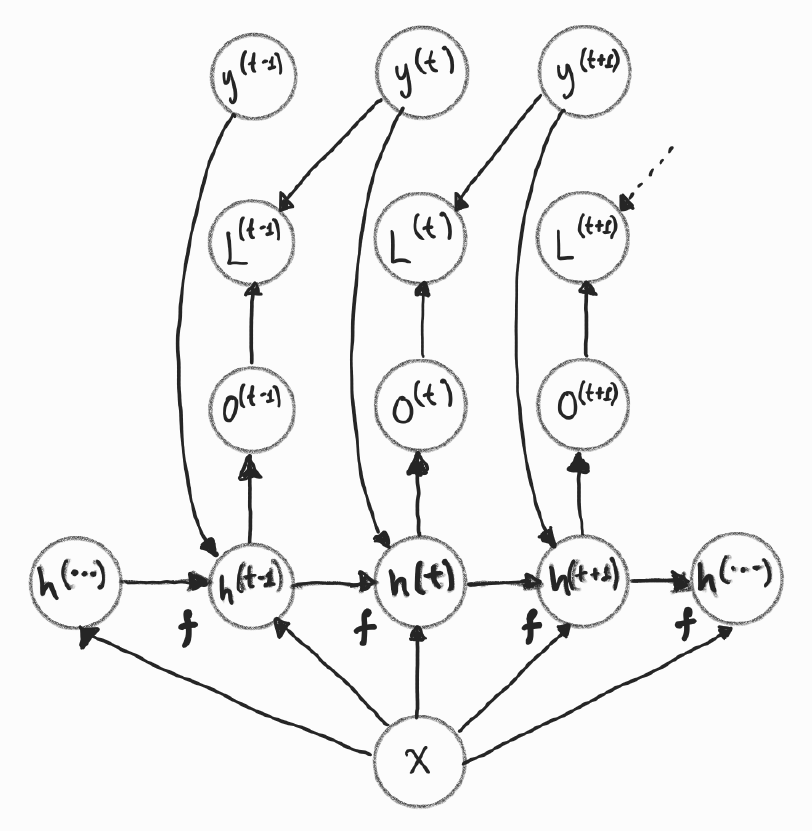
\includegraphics[width=.4\textwidth]{Chapters/2. Transformer/Figures/rnn/rnn_cfge.png}
\caption[RNN - Image Captioning]{Modelo usado para tareas de \textit{Image Captioning}, la entrada es una
sola imagen y la red predice una secuencia de palabras que describen dicha imagen La salida esperada
$y^{(t)}$ sirve como objetivo para la función de costo del paso anterior y como entrada en cada paso.}
\label{fig:rnn_cfge}
\end{figure}


Los modelos ejemplificados anteriormente son construidos de forma \textit{causal}, es
decir, la secuencia es procesada en un solo sentido en donde la información pasada es transmitida
hacia estados futuros. Sin embargo, este flujo de información puede ser insuficiente para resolver
todas las tareas. En \textit{Modelo de Lenguaje} se aprende la estructura estadística del lenguaje con el
que fue entrenado y su meta es predecir la siguiente palabra, n-grama o letra dado un contexto antes
visto. En otros términos, dada una secuencia de texto de longitud
$T$ $x^{(1)}, x^{(2)}, ..., x^{(T)}$
con $x \in \mathcal{R}^{1 \times d}$ donde $d$ es la dimensión de la codificación de las palabras,
la meta es predecir la probabilidad conjunta de la secuencia:

\begin{equation}
    P(x^{(1)}, x^{(2)}, ..., x^{(T)}) = \prod_{t=1}^{T} P(x^{(t)} | x^{(t)}, \dots , x^{(t-1)})
\end{equation}

Con ello, un modelo de lenguaje basado en \textit{Redes Neuronales Recurrentes} es capaz de predecir
un siguiente elemento $\hat x^{(t)}$ simplemente obteniéndolo de la secuencia mediante:

\begin{equation}
    \hat x^{(t)} \approx P(x^{(t)} | x^{(t-1)}, \dots, x^{(1)}) \approx P(x^{(t)} | h^{(t-1)})
\end{equation}

\noindent donde $h^{(t-1)}$ es el estado oculto que almacena la información pasada hasta el tiempo $t$
tal y como se definió en \ref{eq:rnnh}.

Sin embargo, la información previa de la secuencia codificada en $h^{(t)}$ no siempre contiene los
elementos necesarios para que el modelo pueda predecir correctamente el siguiente elemento,
observe la siguiente oración:

\begin{center}
    % \tiny
    << \textit{Ella estaba muy \_\_\_\_\_, después de que Alejandra vió el amanecer en la playa } >>
\end{center}

\noindent en la oración anterior, el espacio en blanco puede ser completado con algún adjetivo calificativo;
\textit{contenta}, \textit{enojada}, \textit{maravillada}, etc. Gracias a la información provista por
la parte final de la oración, podemos deducir que de las 3 opciones la menos probable de
elegir es \textit{enojada}. Es decir, usamos información del futuro que no pudo haber sido vista por
una red (que procesa la información en forma causal) para tomar la mejor elección. Una ligera
modificación fácilmente aplicable a estos modelos es que las secuencias sean procesadas
en ambas direcciones, las \textbf{Redes Neuronales Recurrentes Bidireccionales}
\cite{Schuster}.

Una \textit{RNN Bidireccional} procesa la secuencia en ambos sentidos (una \textit{RNN} en un
sentido y otra en el otro), capturando información del
pasado en el estado oculto $\overrightarrow{h}^{(t)}$  cuando la recurrencia es del inicio al final
de la secuencia e información del futuro en $\overleftarrow{h}  ^{(t)}$ cuando la recurrencia es del
final al inicio de la secuencia. Finalmente, el estado oculto $h^{(t)}$ es una concatenación de ambos
estados $\overrightarrow{h}^{(t)}$ y $\overleftarrow{h}^{(t)}$, vea la ecuación \ref{eq:rrnbi}.
Por lo cual, la salida $o^{(t)}$ ahora puede ser calculada con información tanto del futuro como del pasado
\ref{eq:rrn_out}.

\begin{equation}
\begin{split}
    \overrightarrow{h}^{(t)} = f(x^{(t)}, \overrightarrow{h}^{(t-1)}; \theta_f)\\
    \overleftarrow{h}^{(t)} = f(x^{(t)}, \overleftarrow{h}^{(t+1)}; \theta_b)\\
    h^{(t)} = Concat(\overrightarrow{h}^{(t)}, \overleftarrow{h}^{(t)})
\end{split}
\label{eq:rrnbi}
\end{equation}

\begin{equation}
        o^{(t)} = g(h^{(t)}; \theta_{out})
\label{eq:rrn_out}
\end{equation}


% Compuertas LSTM y GRU
\subsection{Compuertas LSTM y GRU}

Hasta el momento, se ha hecho mención de las salidas $o^{(t)}$ y estados ocultos $h^{(t)}$ solo como
el resultado de operaciones aplicadas por dos funciones: $g$ y $f$, respectivamente. Existen varias
alternativas para construir una \textit{RNN}; una de las maneras más comunes es usando
\ref{eq:rnn_Ht} y \ref{eq:rnn_Ot}:


\begin{equation}
    h^{(t)} = \phi(x^{(t)} W_{x} + h^{(t-1)} W_h + b)
    \label{eq:rnn_Ht}
\end{equation}

\begin{equation}
    o^{(t)} = x^{(t)} W_{out} + b
    \label{eq:rnn_Ot}
\end{equation}

Los parámetros compartidos de la red ahora son descritos por las matrices
$W_x \in \mathbb{R}^{d \times k}$, $W_h \in \mathbb{R}^{k \times k}$ y
$W_{out} \in \mathbb{R}^{k \times q}$ con $k$ como la dimensión del estado oculto, $q$ la dimensión
de las salidas $o^{(t)}$, $b \in \mathbb{R} ^ {1 \times q}$ el parámetro de sesgo y $\phi$ es la
función de activación. De esta manera, los pesos de los parámetros aprendidos en la matriz $W_h$
determinan cómo será usada la información del pasado, codificada en $h^{(t-1)}$. Posteriormente,
es incluida a la codificación de la información del tiempo actual $t$ calculada por $W_x$.
La figura \ref{fig:rnn_cell} representa gráficamente la lógica usada para calcular los estados
ocultos y las salidas de la red.

\begin{figure}[ht!]
\centering
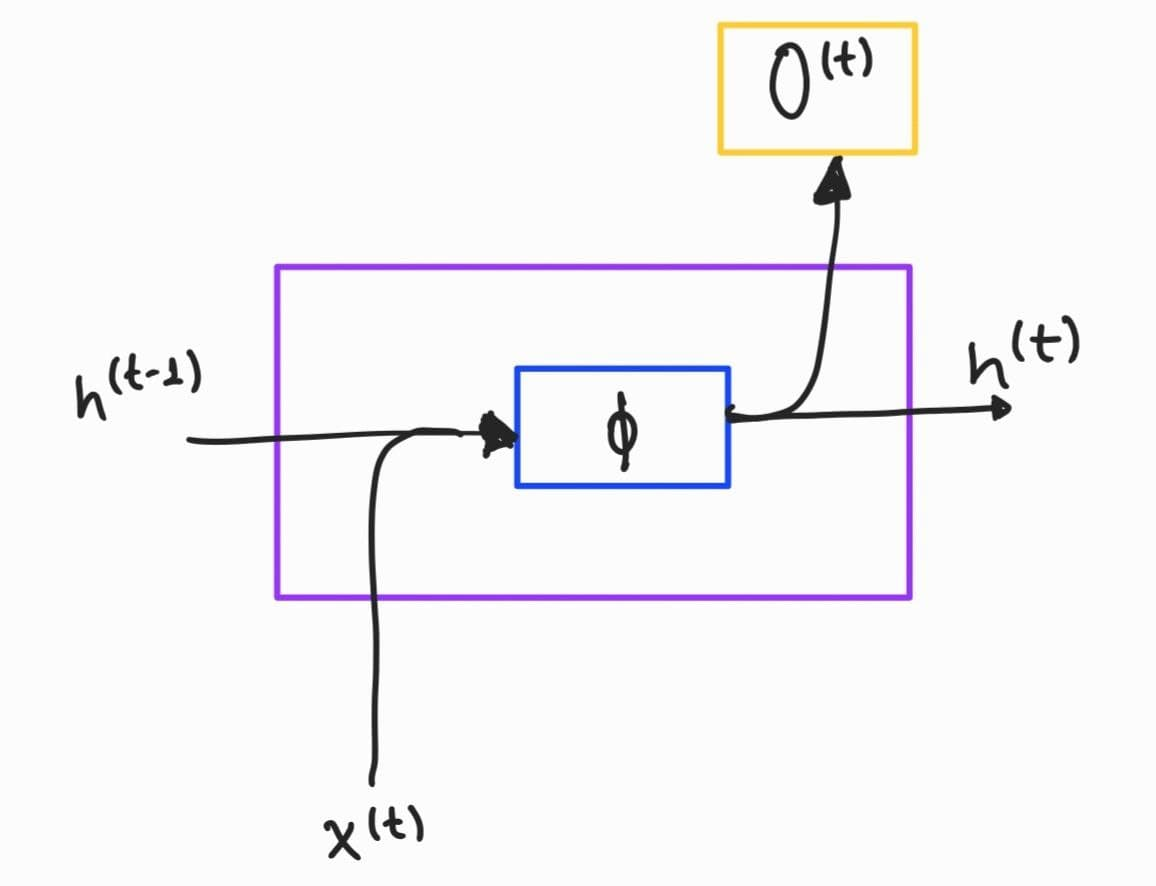
\includegraphics[width=0.4 \textwidth]{Chapters/2. Transformer/Figures/rnn/rnn_cell.jpg}
\caption{Cómputo del estado oculto y salida de una Red Neuronal Recurrente.}
\label{fig:rnn_cell}
\end{figure}

Sin embargo, el cálculo de los estados ocultos mediante \ref{eq:rnn_Ht} presenta algunos problemas.
La interacción entre la información del pasado y la actual siempre es \quotes{plana}, es decir, la información
fluye a través del tiempo de la misma manera sin forma de dar prioridad o ignorar parte de
esta. Por lo tanto, resulta una tarea un poco más complicada preservar información relevante en cada paso
o desechar información que ya no es útil para la red. Además, debido a este mismo flujo de los
datos, la información del pasado poco a poco es opacada por nueva información, impidiendo que se
puedan encontrar dependencias de información en secuencias largas en tiempos distantes;
comúnmente se hace referencia a este problema como \textit{The Short-term Memory Problem} en inglés
\cite{VanishinGradient2}, aunado a problemas como el
\textit{Desvanecimiento o Explosión del Gradiente} \cite{VanishinGradient} \cite{pmlr-v28-pascanu13},
y acentuándose aún más
debido a las matrices de pesos compartidos en la recurrencia. Dichas
multiplicaciones de las matrices en la recurrencia tienen similitud a las realizadas en el
\textit{método de potencia}, en donde cualquier
componente en la matriz inicial que no esté alineada con el vector propio asociado al mayor valor
propio es eventualmente descartado \cite[pp.~390-392]{GoodBengCour16}. Por ende, los resultados
de este producto tenderán a ser cercanos a cero (desvanecerse) o explotar dependiendo de la magnitud
de la matriz de pesos.


Una manera de solventar los problemas anteriores son las \textbf{Redes Neuronales con Compuertas},
creadas con la idea de establecer conexiones a través del tiempo de tal manera que los gradientes no
se desvanezcan ni exploten, convirtiéndose además en un mecanismo para olvidar información pasada y
decidir automáticamente cuándo y cuánto de la información debe prevalecer.


\subsubsection{LSTM}

\textbf{Long Short-Term Memory} (\textbf{LSTM}, por sus siglas en inglés) fue propuesta en 1997 por
\citeauthor{LSTM} como un método para preservar dependencias de información relevante
a corto y largo plazo. Las \textit{LSTM} introducen un nuevo componente: la
\textit{Celda de Memoria}, cuya función es guardar información a través del tiempo y es
controlada por distintas compuertas. Las compuertas aprenden a distinguir qué información es relevante y
cuál no. Hay tres de ellas: la \textit{Compuerta de Entrada}, la \textit{Compuerta de Olvido}
y la \textit{Compuerta de Salida}. La \textit{Compuerta de Entrada} $I^{(t)}$ (véase la figura
\ref{fig:rnn_lstm}) determina cuánta información actual debe ser contemplada a través de la
\textit{Memoria Candidata} $\tilde{C}^{(t)}$ para actualizar la \textit{Celda de Memoria} $C^{(t)}$.
La \textit{Compuerta de Olvido} $F^{(t)}$ indica qué información del pasado debe ser desechada de la
\textit{Celda de Memoria} $C^{(t-1)}$, y la \textit{Compuerta de Salida} ayuda a determinar el nuevo
estado $h^{(t)}$ vía la \textit{Celda de Memoria} actual $C^{(t)}$.


\begin{figure}[ht!]
\centering
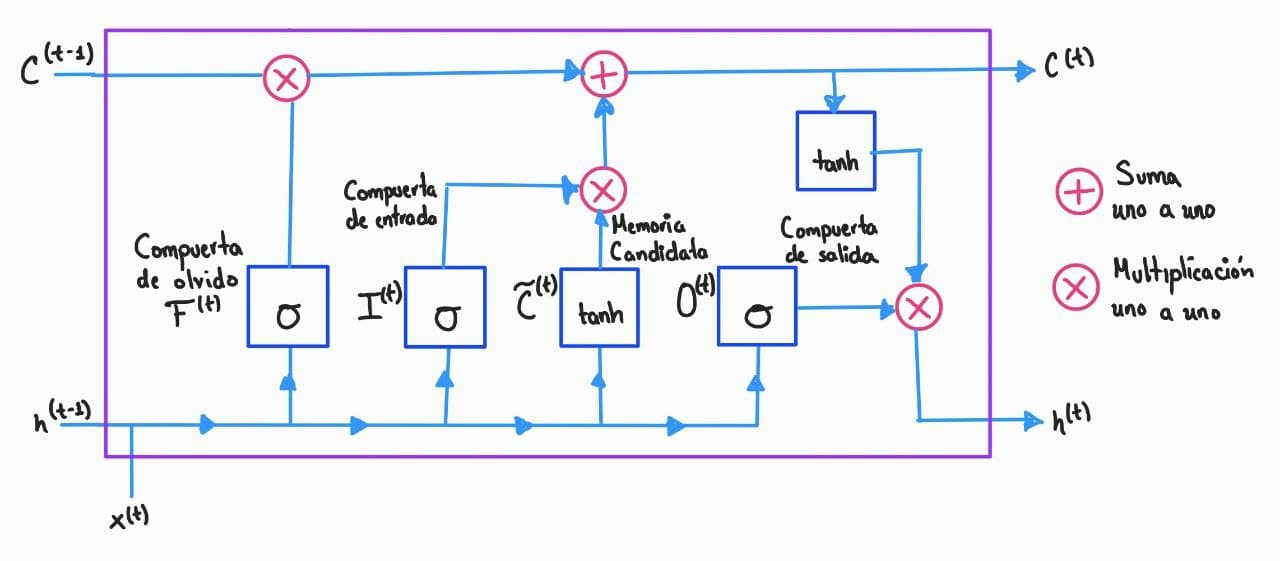
\includegraphics[width=1.0 \textwidth]{Chapters/2. Transformer/Figures/rnn/lstm.jpg}
\caption{LSTM. La \textit{Compuerta de Entrada} $I^{(t)}$ determina cuánta información actual debe
         ser considerada a través de la \textit{Memoria Candidata} $\tilde{C}^{(t)}$ para actualizar
         la \textit{Celda de Memoria} $C^{(t)}$. La \textit{Compuerta de Olvido} $F^{(t)}$ indica
         qué información del pasado debe ser desechada de la \textit{Celda de Memoria} $C^{(t-1)}$,
         y la \textit{Compuerta de Salida} $O^{(t)}$ ayuda a determinar el nuevo estado $h^{(t)}$ a
         través de la \textit{Celda de Memoria} actual $C^{(t)}$.}
\label{fig:rnn_lstm}
\end{figure}

Las ecuaciones \ref{eq:comp} rigen el comportamiento de Compuertas de Entrada, Salida y Olvido,

\begin{equation}
    \begin{split}
        I^{(t)} =  \sigma(x^{(t)} W_{xi} + h^{(t-1)} W_{hi} + b_i)\\
        F^{(t)} =  \sigma(x^{(t)} W_{xf} + h^{(t-1)} W_{hf} + b_f)\\
        O^{(t)} =  \sigma(x^{(t)} W_{xo} + h^{(t-1)} W_{ho} + b_o)\\
    \end{split}
    \label{eq:comp}
\end{equation}

\noindent donde $W_{xi}, W_{xf}, W_{xo} \in \mathbb{R}^{d \times k}$,
$W_{hi}, W_{hf}, W_{ho} \in \mathbb{R}^{k \times k}$ y $b_i, b_f, b_o \in \mathbb{R}^{1xk}$

La Memoria Candidata y la Celda de memoria son actualizadas mediante:

\begin{equation}
    \begin{split}
        \tilde C^{(t)} =  \tanh(x^{(t)} W_{xi} + h^{(t)} W_{hc} + b_c)\\
        C^{(t)} =  F^{(t)} \odot C^{(t-1)} + I^{(t)} \odot \tilde C^{(t)} \\
    \end{split}
\end{equation}

\noindent donde $W_{xi} \in \mathbb{R}^{d \times k}$,
$W_{hc} \in \mathbb{R}^{k \times k}$ y $b_c \in \mathbb{R}^{1xk}$

\noindent y finalmente el estado oculto $h^{(t)}$ esta dado por:

\begin{equation}
    \begin{split}
        h^{(t)} =  O^{(t)} \odot \tanh(C^{(t)}) \\
    \end{split}
\end{equation}

\noindent $\sigma$ y $\odot$ denotan la función de activación sigmoide y la multiplicación uno a uno
respectivamente.


\subsubsection{GRU}

\textbf{Gated Recurrent Units} (\textbf{GRU}, por sus siglas en inglés) fueron propuestas en 2014
\cite{GRU1} como una alternativa computacionalmente más rápida y con rendimiento similar al de las
\textit{LSTM} \cite{GRU2}. A diferencia de estas últimas, las \textit{GRU} prescinden de la
\textit{Celda de Memoria} y utilizan un par de compuertas (la \textit{Compuerta de Actualización} y
la \textit{Compuerta de Olvido}) para decidir qué información aún es necesaria que esté codificada dentro del
estado oculto, véase la ecuación \ref{eq:gru_gates}.
La \textit{Compuerta de Olvido} permite decidir qué del pasado aún debe ser transmitido a futuros
estados o, de otro modo, ser desechada. La \textit{Compuerta de Actualización} indica qué información nueva es relevante y
necesita ser incorporada al no estar codificada dentro del estado oculto,
véase la ecuación \ref{eq:gru_out}.


\begin{equation}
    \begin{split}
        R^{(t)} = \sigma(x^{(t)} W_{xR} + h^{(t-1)} W_{hR} + b_R)\\
        Z^{(t)} = \sigma(x^{(t)} W_{xZ} + h^{(t-1)} W_{hZ} + b_Z)
    \end{split}
    \label{eq:gru_gates}
\end{equation}

\begin{equation}
    \begin{split}
        \tilde h^{(t)} = \tanh(x^{(t)} W_{xh} + ( R^{(t)} \odot h^{(t-1)}) W_{hh} + b_h)\\
        h^{(t)} =  Z^{(t)} \odot h^{(t-1)} + (1 - Z^{(t)}) \odot \tilde h^{(t-1)} \\
    \end{split}
    \label{eq:gru_out}
\end{equation}

\begin{figure}[ht!]
\centering
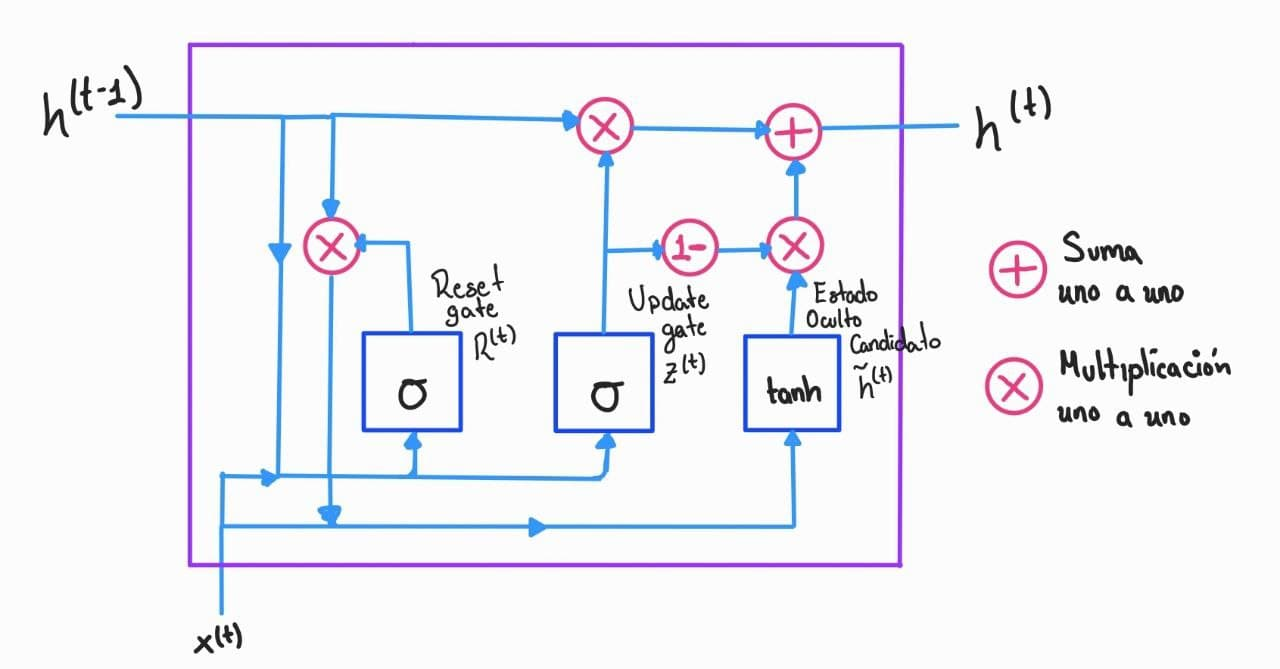
\includegraphics[width=1.0 \textwidth]{Chapters/2. Transformer/Figures/rnn/GRU.jpg}
\caption{GRU. A diferencia de las \textit{LSTM}, las \textit{GRU} prescinden de la
         \textit{Celda de Memoria} y utilizan un par de compuertas (la \textit{Compuerta de
         Actualización} y la \textit{Compuerta de Olvido}) para decidir qué información es necesaria
         que esté codificada dentro del estado oculto.}
\label{fig:rnn_gru}
\end{figure}


% Modelos de atención
\subsection{Mecanismos de atención} \label{section:att}

Una de las arquitecturas comunes vistas previamente es la mostrada en la figura \ref{fig:rnn_cfgc}, cuya información
procesada es resumida en una sola salida. Este tipo de red es usada como parte de las soluciones en
tareas de reconocimiento de voz (\textit{Speech Recognition}), traducción de lenguaje
(\textit{Machine Translation}) o asistencia en respuestas automáticas (\textit{Question Answering}), entre
otros,
típicamente bajo modelos Secuencia a Secuencia (\textit{Sequence to Sequence, Seq2Seq})
\cite{DBLP:journals/corr/ChoMGBSB14}. Los modelos
\textit{Seq2Seq} están formados por dos redes neuronales como la mostrada en \ref{fig:seq2seq}. La
primera se comporta como un \textit{codificador} al resumir la entrada y producir un vector de salida
de tamaño fijo llamado \textit{vector de contexto}. La segunda red se comporta como un
\textit{decodificador}, que es inicializado y condicionado con el
\textit{vector de contexto} para obtener una transformación de la entrada no necesariamente del
mismo tamaño de secuencia, debido a que en tareas como traducir una oración de un lenguaje a otro,
la traducción no siempre contiene la misma cantidad de palabras usadas en el idioma original.


\begin{figure}[ht!]
    \centering
    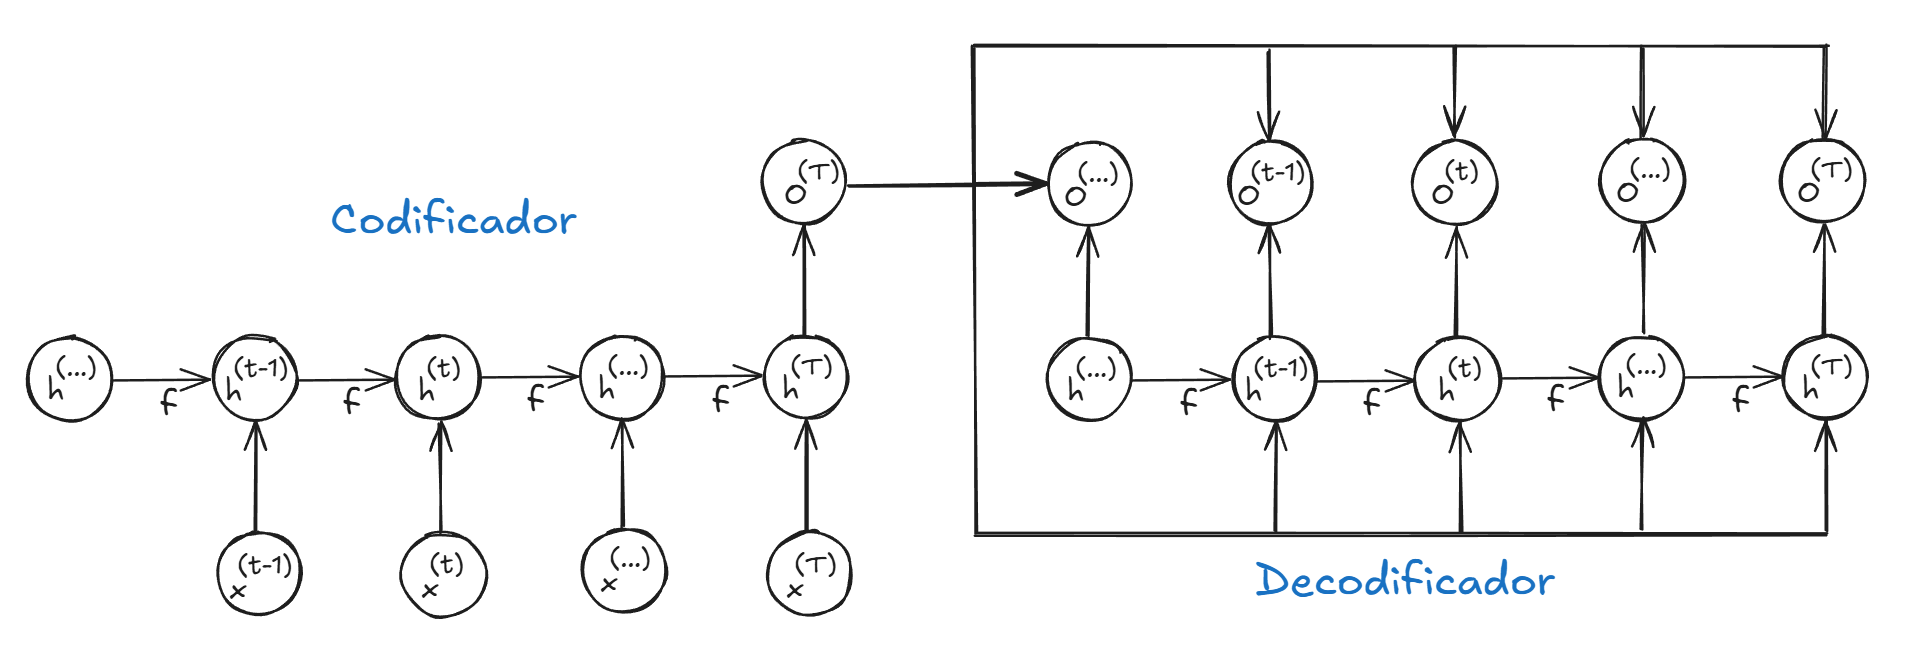
\includegraphics[width=1.0 \textwidth]{Chapters/2. Transformer/Figures/rnn/seq2seq.png}
    \caption{Seq2Seq. Modelos seq2seq. Estos modelos transforman una secuencia de entrada en una
             secuencia de salida utilizando un codificador y un decodificador. Son ampliamente
             utilizados en tareas como la traducción automática, el resumen de texto y la generación
             de diálogos.}
    \label{fig:seq2seq}
\end{figure}

Por ejemplo, en tareas de \textit{Machine Translation} el \textit{codificador} esta formado por una
\textit{RNN} Bidireccional que lee y procesa un conjunto de
vectores $X = (x^{(1)}, x^{(2)}, \dots, x^{(T_x)})$ para obtener un vector de contexto $C$. La forma
más común es como en \ref{eq:s2s_simple}:

\begin{equation}
    \begin{split}
        h^{(t)} = f_{bi}(x^{(t)}, h^{(t-1)}; \theta_{f}, \theta_{b}) \\
        C = q({h^{(1)}, h^{(2)}, \dots, h^{(T)}})
    \end{split}
    \label{eq:s2s_simple}
\end{equation}

Recordemos que $h^{(t)}$ es el estado oculto generado por la concatenación de los dos estados
ocultos generados por la \textit{RNN Bidireccional}. Las funciones $f_{bi}$ y $q$ son no lineales,
siendo $f_{bi}$ una \textit{LSTM} y $q(h^{(1)}, h^{(2)}, \dots, h^{(T)}) = h^{(T)}$, equivalente a
tomar solo el último estado oculto como vector de contexto $C$. El \textit{decodificador} se entrena
para predecir la siguiente palabra $y^{(t')}$ dado el vector de contexto $C$ y todas las palabras
previas predichas. En otras palabras, el decodificador define la probabilidad conjunta modelada por
una \textit{RNN}:

\begin{equation}
    p(Y) = \prod_{t=1}^{T_y} p(y^{(t)} | \{y^{(1)}, \dots , y^{(t-1)}\}, C)
\end{equation}
\begin{equation}
    p(y^{(t)} | \{y^{(1)}, \dots , y^{(t-1)}\}, C) = g(y^{(t-1)}, s^{(t)}, C; \theta_g)
\end{equation}

\noindent donde $g$ es una función no lineal que emite la probabilidad de $y^{(t)}$ y $s^{(t)}$ es el
estado oculto del \textit{decodificador} \ref{eq:sqs_s}.

\begin{equation}
    s^{(t)} = f(s^{(t)}, y^{(t-1)}, C; \theta_s)
    \label{eq:sqs_s}
\end{equation}


Sin embargo, cuando las secuencias son bastante largas, el \textit{vector de contexto} emitido por el
\textit{codificador} no es lo suficientemente grande como para resumir correctamente la secuencia.
Por tanto, la información inicial de la entrada es olvidada, teniendo escasa presencia en estados
ocultos más lejanos. En 2015, \citeauthor{bahdanau2016neural} observaron estos efectos y propusieron
una forma de minimizarlos: los \textbf{Mecanismos de Atención}.

La función principal de los \textbf{Mecanismos de Atención} es permitir que el \textit{decodificador}
pueda acceder al historial completo de los estados ocultos del \textit{codificador}. Así, ahora podrá
contar con un mecanismo para centrarse selectivamente en las distintas partes de la secuencia que
tienen mayor influencia sobre la salida esperada en cierto tiempo.

Es así que las palabras predichas no son calculadas por un único \textit{vector de contexto} generado
por el \textit{codificador}, sino que para cada objetivo $y^{(t)}$ se calcula un nuevo \textit{vector
de contexto} $c^{(t)}$:


\begin{equation}
    p(y^{(t)} | \{y^{(1)}, \dots , y^{(t-1)}\}, c^{(t)}) = g(y^{(t-1)}, s^{(t)}, c^{(t)}; \theta_g)
\end{equation}

\begin{equation}
    s^{(t)} = f(s^{(t)}, y^{(t-1)}, c^{(t)}; \theta_s)
\end{equation}

Dado que cada estado oculto $h^{(t)}$ contiene mejor la información que se encuentra alrededor del
t-ésimo término, se puede generar cada vector de contexto como una suma ponderada sobre los estados
ocultos del \textit{codificador}. Estos pesos nos ayudan a determinar qué tan importante es la
información codificada por cada estado oculto y, al momento de obtener la salida del t-ésimo valor,
\quotes{prestar atención} a aquellos que son más relevantes para esta predicción:


\begin{equation}
    c^{(t)} = \sum_{i=1}^{T_x} \alpha_{t,i} h^{(i)}
\end{equation}

\noindent aquí cada peso $\alpha_{t,i}$ indica qué tan bien se \quotes{alinean} los términos $y^{(t)}$ y $x^{(i)}$,
y son calculados por una \textit{función de alineamiento} que denota qué tan importante es el estado
oculto del \textit{codificador} $h^{(t)}$ para el estado oculto del \textit{decodificador} $s^{(i)}$.


\begin{equation}
    \alpha_{t,i} = align(y^{(t)}, x^{(i)}) = \frac{\exp(score(s^{(t-1)}, h^{(i)}))}{\sum_{k=1}^{T_x} \exp(score(s^{(t-1)}, h^{(k)}))}
    \label{eq:b_align}
\end{equation}

\textit{Bahdanau} propone aprender esta alineación usando una \textit{red feed-forward} con una sola
capa oculta y la función $\tanh$ como activación:

\begin{equation}
    score(s^{(t)}, h^{(i)}) = v^\top_a \tanh(W_a[s^{(t)};h^{(i)}])
    \label{eq:concat}
\end{equation}

\noindent con $v_a$ y $W_a$ como matrices de pesos a aprender durante el entrenamiento, $[s^{(t)};h^{(i)}]$
representa una concatenación de los estados ocultos del \textit{codificador} y \textit{decodificador}.
En la figura \ref{fig:att} podemos ver gráficamente el modelo usado por \textit{Bahdanau}.

\begin{figure}[ht!]
    \centering
    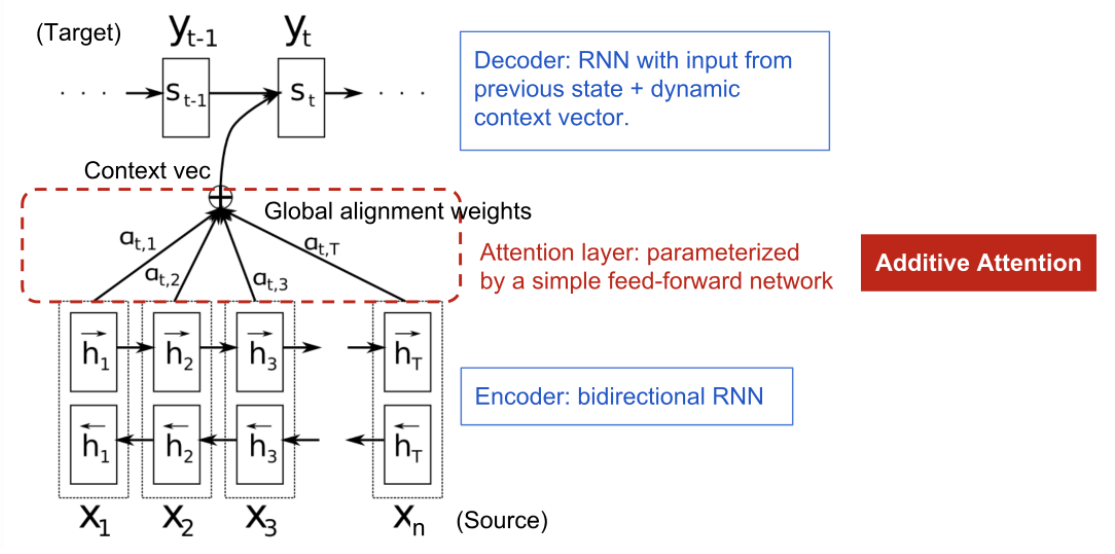
\includegraphics[width=0.8 \textwidth]{Chapters/2. Transformer/Figures/rnn/attention.png}
    \caption{Modelo seq2seq propuesto por \citeauthor{bahdanau2016neural} con \textit{Additive/Concat Attention}}
    \label{fig:att}
\end{figure}

Los modelos de atención pueden ser vistos de manera más general como un mapeo de una secuencia de
llaves $k$ hacia una distribución de atención $\alpha$ de acuerdo a una consulta $q$, aplicándose a
un conjunto de valores $V$ para selectivamente propagar la información contenida en $V$. Si bien los
términos de consulta, llaves y valores (query, keys, values) son propios de los \textit{Sistemas de
Recuperación de Información}, su relación en términos de la atención aplicada por Bahdanau es muy
similar; las llaves son los estados ocultos del \textit{codificador} y la consulta es el estado
oculto del \textit{decodificador} en cuestión. En este caso, el mapeo entre llaves y valores es el mismo:


\begin{equation}
    A(q, K, V) = \sum_i p(a(K-i, q)) * v_i
    \label{eq:att_general}
\end{equation}

En la ecuación \ref{eq:att_general}, $p$ es una función de distribución que mapea los puntajes de la
función de alineación $a$ a pesos de atención. Comúnmente se usan las funciones \textit{softmax} o
\textit{logistic sigmoid} puesto que nos aseguran que los pesos de atención producidos estarán dentro
del rango $[0,1]$ y la suma de ellos es igual a $1$, por lo que los pesos pueden ser interpretados
como una probabilidad que indica qué tan relevante es cierto elemento. Algunas variaciones en donde
se consideran solo los términos relevantes, como \textit{sparsemax} \citeauthor{DBLP:journals/corr/MartinsA16}
o \textit{sparse entmax} \citeauthor{DBLP:journals/corr/abs-2006-07214}, permiten trabajar y enfocarse
en solo algunas relaciones de alineamiento. \citeauthor{NEURIPS2019_16fc18d7} proponen una función de
distribución de pesos $M = \tanh(E) \odot sigmoid(N)$ con $E$ como una matriz en donde cada entrada
representa la similaridad entre estados ocultos y $N$ una medida negativa (disimilaridad), por lo que
podemos usar $sigmoid(N)$ como información para \quotes{de-atender} los alineamientos de $E$.


Las funciones de alineamiento se encargan de comparar y extraer la relación entre las representaciones
de las llaves (keys) y consultas (queries), por ejemplo, usando el producto punto y el coseno como
función de similaridad. Bahdanau calcula esta relación a través de una red neuronal \ref{eq:b_align},
lo que evita asumir que ambas representaciones están en el mismo espacio, como lo hacen las funciones
de alineación como el producto punto o la similaridad coseno. La tabla \ref{Tab:att} muestra una
recopilación de funciones de alineamiento.


\begin{table}[ht!]
\begin{center}
\resizebox{\textwidth}{!}{
\begin{tabular}{@{}lll@{}}
\toprule
\textbf{Nombre} & \textbf{Función de Alineación} & \textbf{Cita} \\
\midrule
Similarity / Content-Base & $a(k_i, q) = sim(k_i, q)$ & \citeauthor{DBLP:journals/corr/GravesWD14} \\ \\
Dot Product\textsuperscript{1} & $a(k_i, q) = q^\top k_i$ & \citeauthor{DBLP:journals/corr/LuongPM15} \\ \\
Scaled Dot Product & $a(k_i, q) = \frac{q^\top k_i}{\sqrt{d_k}}$ & \citeauthor{DBLP:journals/corr/VaswaniSPUJGKP17} \\ \\
General & $a(k_i, q) = q^\top W k_i$ & \citeauthor{DBLP:journals/corr/LuongPM15} \\ \\
Biased General & $a(k_i, q) = k_i (Wq + b )$ & \citeauthor{DBLP:journals/corr/SordoniBB16} \\ \\
Activated General & $a(k_i, q) = act(q^\top W k_i + b)$ & \citeauthor{DBLP:journals/corr/abs-1709-00893} \\ \\
Generalized Kernel & $a(k_i, q) = \phi(q)^\top \phi(k_i)$ & \citeauthor{DBLP:journals/corr/abs-2009-14794} \\ \\
Additive\textbackslash Concat \textsuperscript{2} & $a(k_i, q) = v^\top act(W[q;k_i]+ b)$ & \citeauthor{bahdanau2016neural}, \citeauthor{DBLP:journals/corr/LuongPM15} \\ \\
Deep & $a(k_i, q) = v^\top E^{(L-1)} + b^L$ & \citeauthor{Pavlopoulos} \\
    & $E(l) = act(W_l E^{(l-1)} + b^l)$ &  \\
    & $E(1) = act(W_0k_i + W_1q + b^l)$ &  \\ \\
Location-based & $a(k_i, q) = act(W q)$ & \citeauthor{DBLP:journals/corr/LuongPM15} \\ \\
Feature-based & $a(k_i, q) = v^\top act(W_0 \phi(K) + W_1 \phi(K) + b)$ & \citeauthor{DBLP:journals/corr/abs-1810-10126} \\
\bottomrule
\end{tabular}}
\end{center}
\caption{Distintos tipos de funciones de alineación. (Tabla basada en \cite{DBLP:journals/corr/abs-1904-02874} y \cite{weng2018attention}). \\
$a(k_i, q)$ representa la función de alineación entre $k_i$ y $q$ y $act$ es una función de activación. \\
$sim$ es una función de similaridad, \citeauthor{DBLP:journals/corr/GravesWD14} propone la función coseno.\\
Los parámetros $v, W, W_1, W_2$ son parámetros aprendidos por la red neuronal.\\
\textsuperscript{1} El factor de escala $\frac{1}{\sqrt{d_k}}$ ayuda a estabilizar cuando el
gradiente es muy pequeño. $d_k$ es el tamaño de la cabeza de atención.\\
\textsuperscript{2} La función de activación propuesta por \citeauthor{bahdanau2016neural} es la función $tanh$ como se ve en \ref{eq:concat} \\
\label{Tab:att}}
\end{table}

De acuerdo a cómo se aplican los distintos tipos de atención, \citeauthor{DBLP:journals/corr/abs-1904-02874}
los dividen en 4 grandes grupos: por número de secuencias, por nivel de abstracción, por número de
posiciones y por número de representaciones. Estos grupos no son mutuamente excluyentes, por lo tanto,
una aplicación de atención puede pertenecer a más de uno.

En la categoría \textit{por número de secuencias} se identifican 3 tipos. El primero de ellos,
\textbf{Distintivos} (\textit{Distinctive}), es cuando la clave (key) y el valor (value) pertenecen a
distintas secuencias de entrada y salida respectivamente, como es el caso del modelo propuesto por
\citeauthor{bahdanau2016neural}. El segundo tipo, \textbf{Co-Atención} (\textit{co-attention}), utiliza
distintas secuencias al mismo tiempo para conocer los pesos de atención entre estas entradas. Por ejemplo,
en tareas donde se necesita trabajar con datos multimodales como procesar imágenes y texto
simultáneamente. En tareas como \textit{Visual Question Answering}, se puede aplicar un mecanismo de
atención conjunto tanto para las imágenes como para el texto, para identificar las regiones de la imagen
y las palabras del texto que son más relevantes. El tercer tipo es \textbf{Auto-Atención} (\textit{Self
Attention}), propuesto por \citeauthor{yang2016hierarchical}, y es uno de los puntos clave para los
modelos \textit{Transformers} \cite{DBLP:journals/corr/VaswaniSPUJGKP17}. Es comúnmente usada en tareas
que solo requieren una salida resumen y no una secuencia, como \textit{Clasificación de texto}. La clave
(key) y el valor (value) pasan a ser los mismos y la atención se calcula sobre los mismos elementos
pertenecientes a la secuencia de entrada, buscando así encontrar las relaciones entre las palabras de la
misma oración.

La segunda categoría agrupa la atención por el nivel de abstracción en el que es aplicada, a un
\textbf{solo nivel} o en \textbf{múltiples niveles}. La información a procesar muchas veces puede ser
representada en distintos niveles de abstracción, es decir, en texto, podemos separar los datos a
nivel de letras, n-gramas, palabras, oraciones, párrafos, etc. Por tanto, es posible atender de manera
jerárquica a las palabras que forman una oración para posteriormente prestar atención a las oraciones
que conforman un texto más largo. \citeauthor{yang2016hierarchical} utiliza este procedimiento para
generar un vector de características usado posteriormente en una etapa de clasificación.

En la tercera categoría, la atención es realizada en diversas partes de la secuencia; la suma ponderada
sobre todos los puntajes de las entradas usada por \citeauthor{bahdanau2016neural} se le denomina
\textbf{Atención suave} (\textit{Soft-Attention}). Una alternativa es la \textbf{Atención dura}
(\textit{Hard-Attention}) \cite{DBLP:journals/corr/XuBKCCSZB15}, que calcula la atención no sobre todos
los puntajes de alineamiento sino en una parte de estos. Para ello, se usa una distribución multinoulli
parametrizada por los pesos de la atención. A pesar de que es más eficiente que la \textit{atención
suave}, resulta difícil de entrenar al no ser completamente diferenciable. Otra opción a la
\textit{atención dura} es la \textbf{Atención Local} (\textit{Local Attention}), cuya idea es aplicar
atención sobre una ventana elegida, ya sea centrada con respecto al tiempo actual (alineamiento
monotónico) o predicha por una función (alineamiento predictivo). La \textit{atención local} fue
propuesta por \citeauthor{DBLP:journals/corr/LuongPM15}, así como la \textit{Atención Global}, la cual
es similar a la \textit{atención suave}.

La última categoría divide los modelos de atención por las formas de representación de las entradas
sobre las que la atención es aplicada. Distintos modelos pueden beneficiarse de procesar los datos
creando vectores de características distintos, cada uno de ellos derivado de algún tipo de representación
de la entrada. Por tanto, es posible atender a diferentes representaciones y formar un vector final
usando una combinación ponderada de estos a través de dichos pesos de atención.
\citeauthor{DBLP:journals/corr/abs-1904-02874} llama a este tipo de modelos de atención
\textbf{multi-representational AM}. En la segunda categoría, \textbf{multi-dimensional attention}, la
atención no es aplicada sobre los diversos vectores de características sino a un nivel más interno,
sobre sus dimensiones. Pesar cada característica de un vector de características permite seleccionar
aquellas que mejor lo describen para un contexto dado. En \textit{NLP}, resulta bastante útil cuando se
trata con \textit{polisemia}, en donde una palabra o frase puede tener más de un significado.


% Transformer
\section{El modelo Transformer}

A finales del año 2017 se presentó un nuevo modelo que vino a revolucionar el área de Procesamiento
de Lenguaje Natural, El Transformer \cite{Vaswani}. Una de sus principales características es la
capacidad de procesar la información de alguna secuencia de forma paralela, caso contrario a las
Redes Neuronales Recurrentes, donde la información se procesa recurrentemente. Gracias a ello,
la capacidad de \textit{recuerdo} no se ve afectado por el problema de \textit{El desvanecimiento
del Gradiente} específicamente cuando el problema es trabajar con secuencias  bastante largas.

\textit{El Transformer} puede ser visto como otro modelo \textit{seq2seq} (Secuencia a Secuencia)
\ref{fig:trans_seq2sqe}, formado en por dos etapas, la primera encargada de codificar la información de entrada
y la segunda de decodificarla, pero su principal característica es que aplica mecanismos de
\textit{Self-Attention} para capturar las dependencias globales entre la entrada y la salida. Dada
una secuencia de entrada $X = (x_1, x_2, \dots, x_n )$ con $n$ como el tamaño de la secuencia,
el codificador produce una representación intermedia
$Z = (z_1, z_2, \dots, z_n)$ al igual que los modelos \textit{seq2seq}. El decodificador usa la
secuencia $Z$ para generar la secuencia de salida
$Y = (y_1, y_2, \dots, y_m)$ uno a la vez (en modo inferencia), con $m$ como el tamaño de la
secuencia de salida. Nótese, que el generar una salida a la vez el decodificador tiene que ser auto-regresivo.
Usa la salida anterior $y_{i-1}$ como entrada adicional para generar la siguiente salida $y_i$. Por
ello, durante entrenamiento el modelo es alimentado con entradas y salidas desfasadas en un tiempo.

\begin{figure}[ht!]
    \centering
    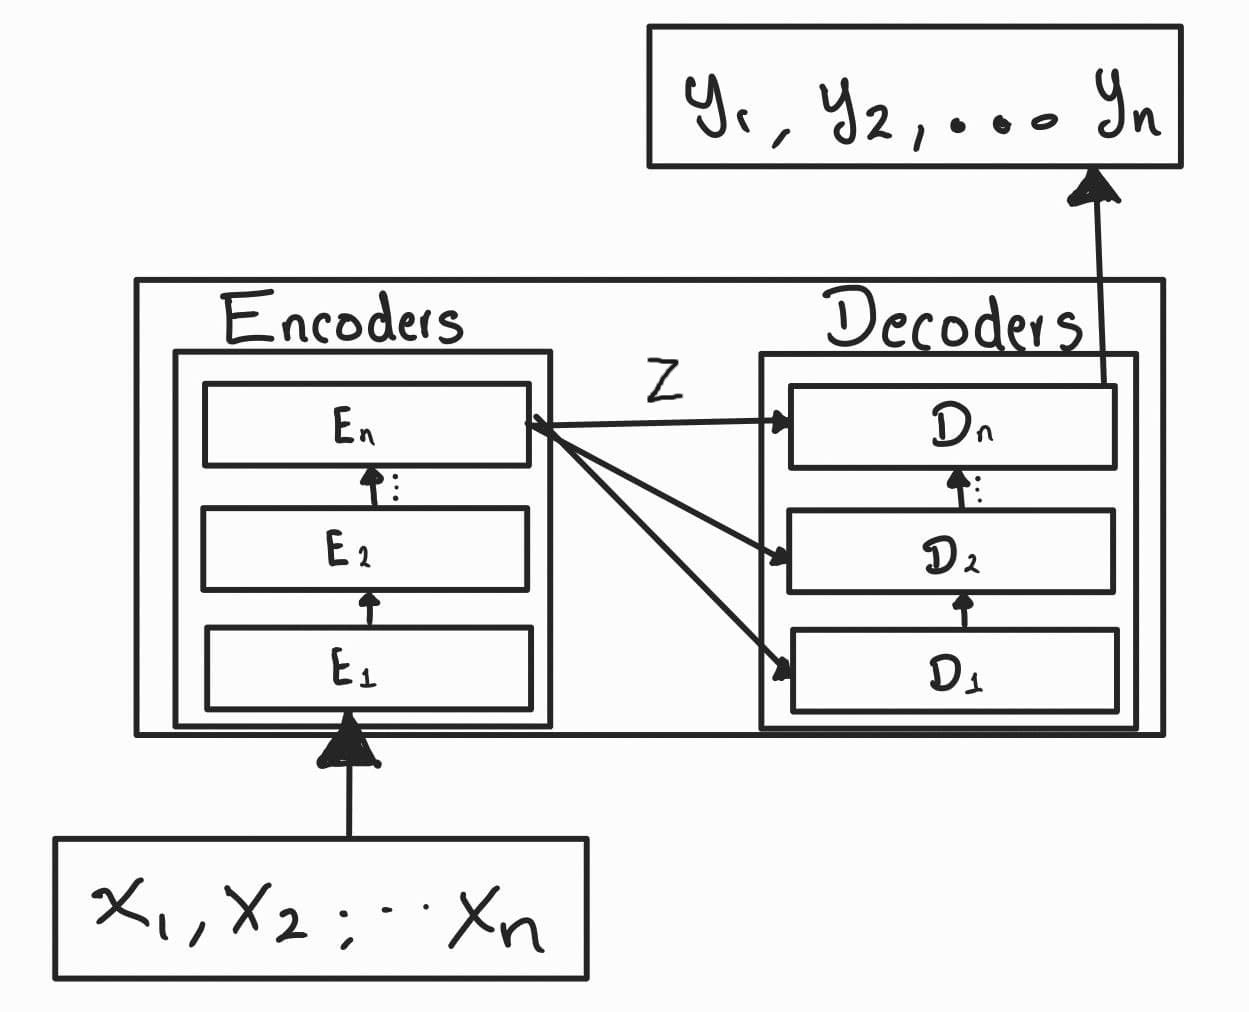
\includegraphics[width=0.4 \textwidth]{Chapters/2. Transformer/Figures/transformer/t_seq2seq.jpg}
    \caption{Modelo Transformer generalizado como modelo Secuencia a Secuencia}
    \label{fig:trans_seq2sqe}
\end{figure}


\subsection{El Codificador y Decodificador}

El \textit{Modelo Transformer} está formado por multiples codificadores  y decodificadores apilados e inter-conectados,
Como observamos en la figura \ref{fig:trans_seq2sqe}. El codificador consta de dos capas,
la primera de ellas aplica \textit{Self-Attention} múltiples veces sobre la misma entrada
(\textit{Multi-HeadSelf Attention}) y la segunda capa representada solo por una red
\textit{Feed-Forward} cuya entrada es la salida de la capa anterior.
Véase la figura \ref{fig:trans_encoder}.


\begin{figure}[ht!]
\centering
    \begin{minipage}{.4\textwidth}
        \centering
        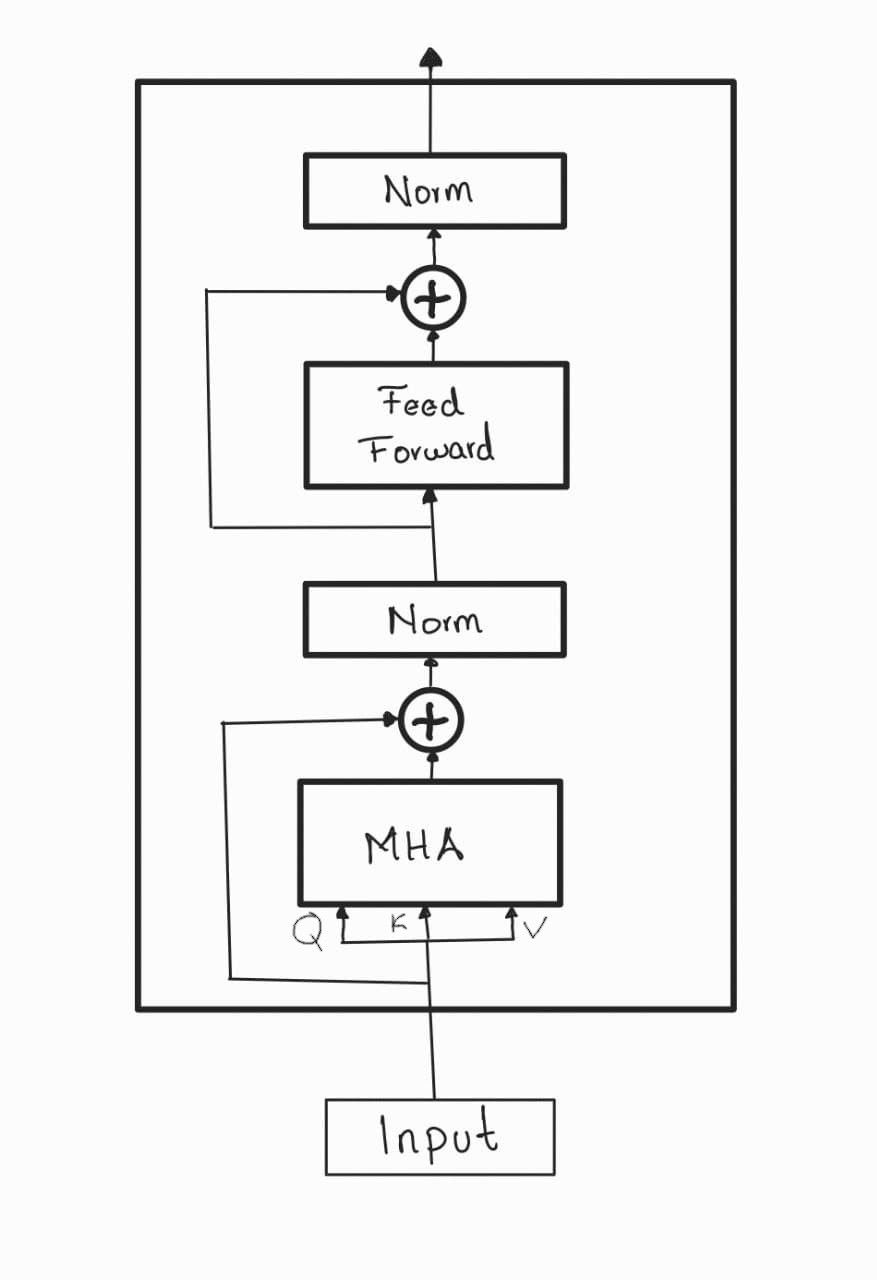
\includegraphics[width=0.7 \textwidth]{Chapters/2. Transformer/Figures/transformer/encoder.jpg}
    \end{minipage}
    \begin{minipage}{.5\textwidth}
        \begin{equation*}
            \begin{split}
                mha = MHA(X, X, X)\\
                norm = Norm( mha + X)\\
                f = FeedForward(norm)\\
                Encoder(X) = Norm(f + norm)
            \end{split}
            \label{eq:trans_enc}
        \end{equation*}
    \end{minipage}
    \caption{Etapa Codificadora del Modelo Transformer. Pseudocódigo}
    \label{fig:trans_encoder}
\end{figure}


El decodificador tiene una estructura similar al codificador con una etapa adicional intermedia
de \textit{Multi-Head Attention} aplicada sobre la salida de la pila de codificadores. También, la
primer capa de atención sufre un ligero cambio un su forma de operación, necesitando enmáscarar (al
momento en que se realiza el entrenamiento) la atención prestada del pasado al futuro. Esto es
debido a que el decodificador se encarga de generar una secuencia (en modo inferencia) uno a la vez
usando solamente la salida anterior y por tanto no tiene conocimiento de salidas futuras, observe
la figura \ref{fig:trans_te}.

\begin{figure}[ht!]
\centering
    \begin{minipage}{.4\textwidth}
        \centering
        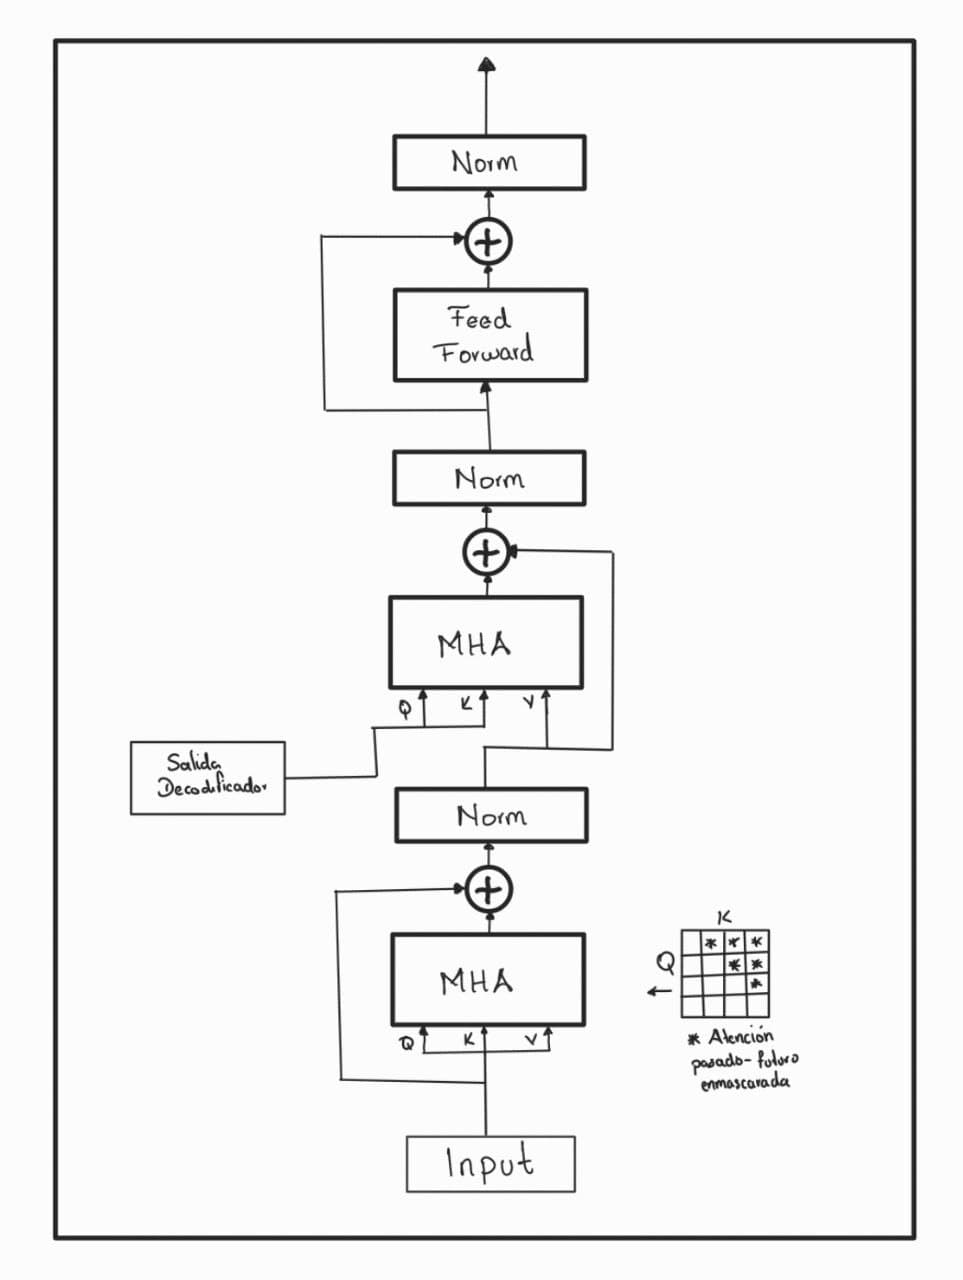
\includegraphics[width=1.0 \textwidth]{Chapters/2. Transformer/Figures/transformer/decoder.jpg}
    \end{minipage}
    \begin{minipage}{.5\textwidth}
        \begin{equation*}
            \begin{split}
                mha_1 = MHA(X, X, X)\\
                norm_1 = Norm( mha_1 + X)\\
                mha_2 = MHA(enc_{out}, enc_{out}, norm_1)\\
                norm_2 = Norm( mha_2 + X)\\
                f = FeedForward(norm_2)\\
                decoder(X) = Norm(f + norm_2)
            \end{split}
            \label{eq:trans_dec}
        \end{equation*}
    \end{minipage}
    \caption{Etapa Decodificadora del Modelo Transformer. Pseudocódigo}
    \label{fig:trans_decoder}
\end{figure}


\begin{figure}[ht!]
    \centering
    \begin{subfigure}[b]{0.49\textwidth}
        \centering
        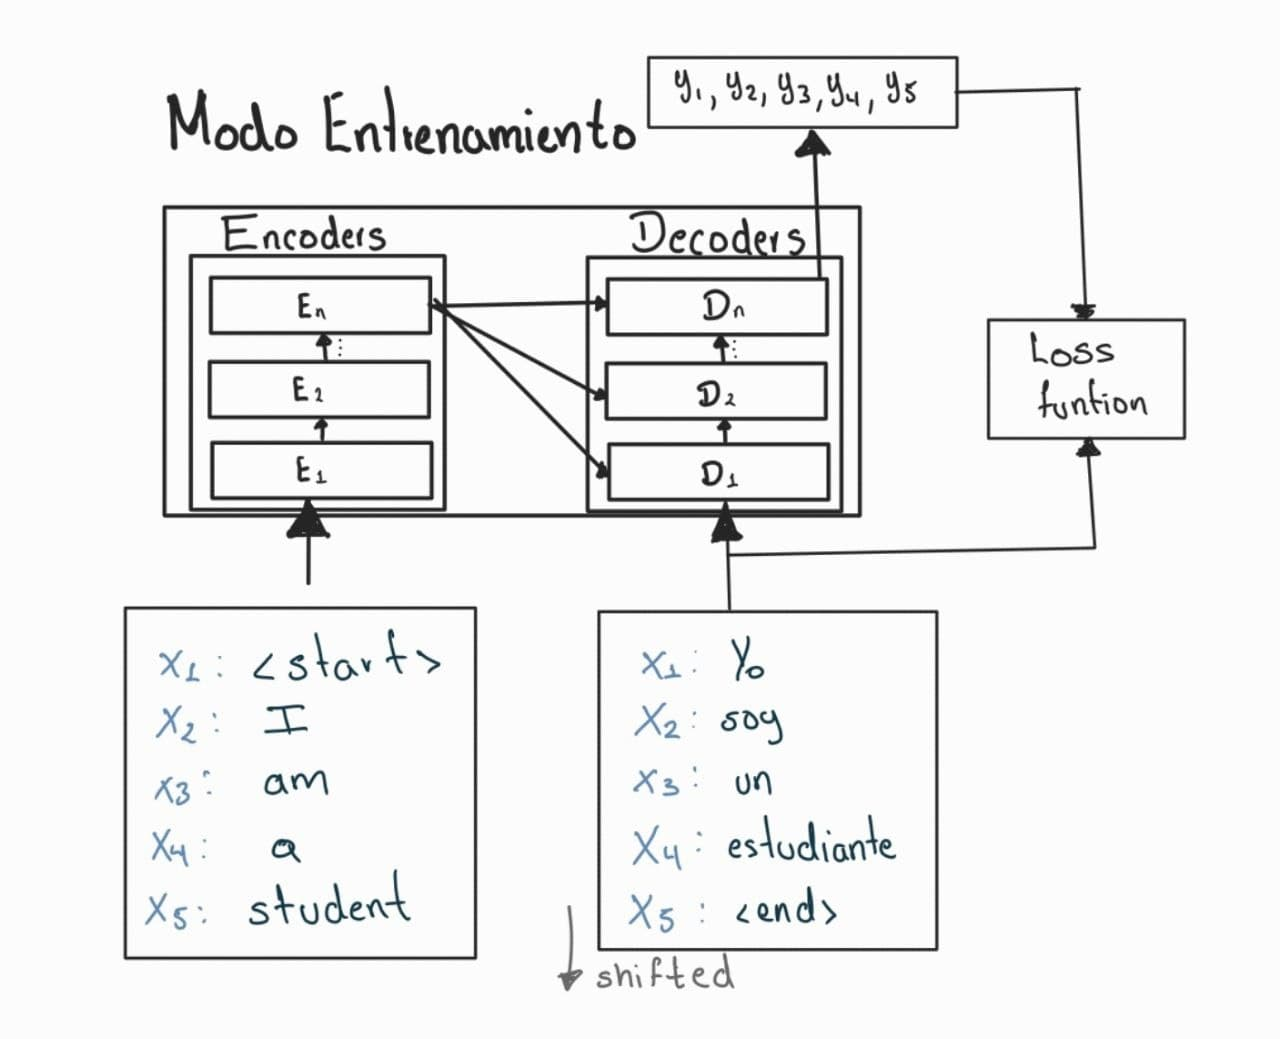
\includegraphics[width=1.0 \textwidth]{Chapters/2. Transformer/Figures/transformer/train.jpeg}
        \caption{Transformer modo entrenamiento. Las entradas en el decodificador son recorridas un
                 elemento en el futuro, con el fin de que aprende a predecir la siguiente palabra
                 dado un contexto previo y las salidas actuales en el momento de la evaluación.}
        \label{fig:trans_train}
    \end{subfigure}
    \begin{subfigure}[b]{0.49\textwidth}
        \centering
        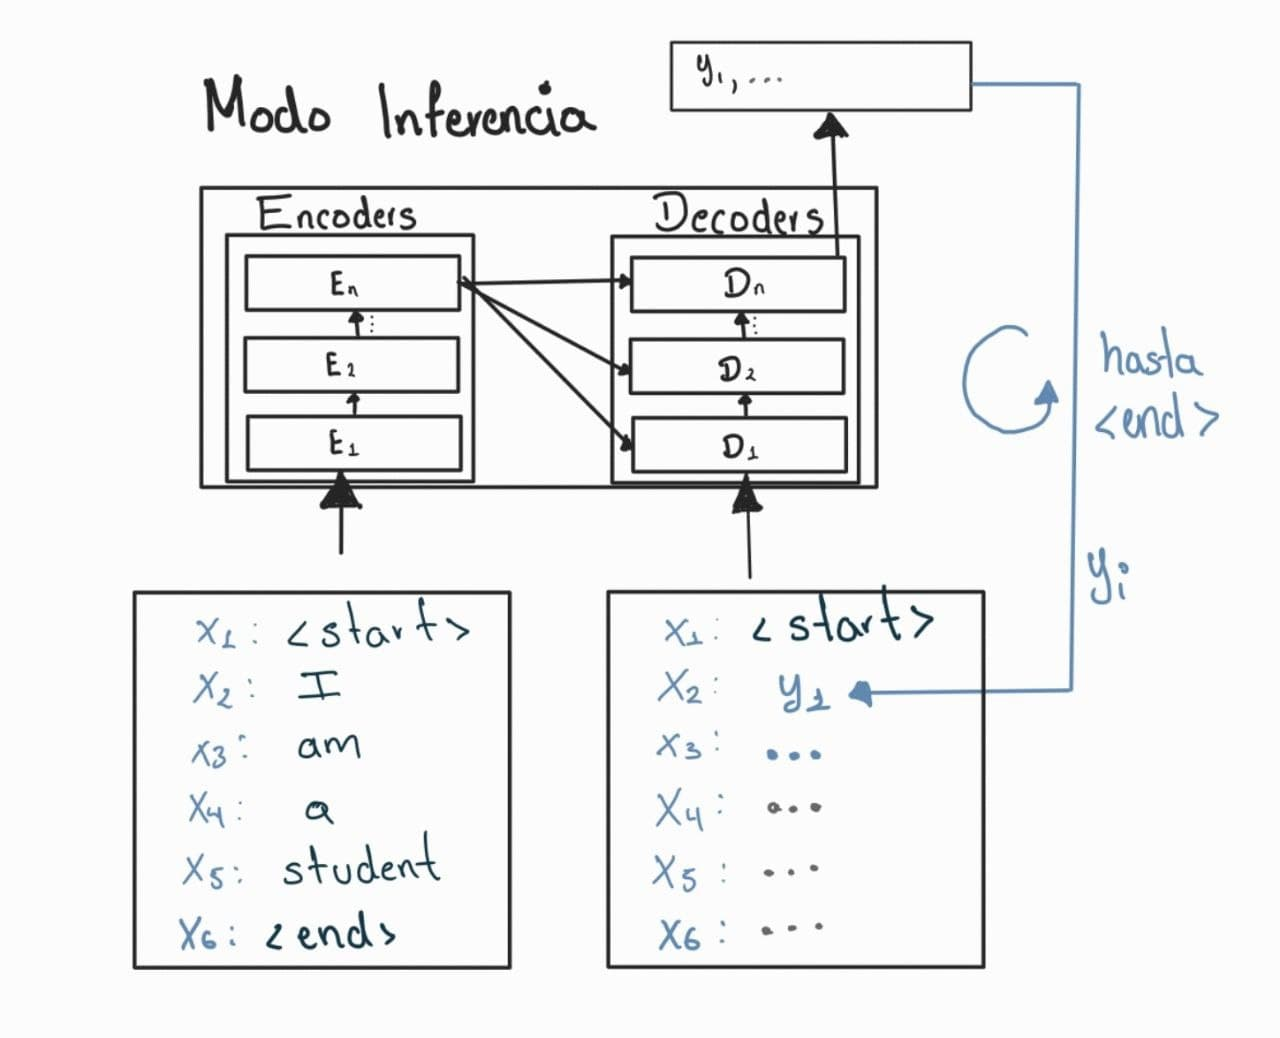
\includegraphics[width=1.0 \textwidth]{Chapters/2. Transformer/Figures/transformer/inference.jpg}
        \caption{Transformer modo inferencia. El decodificador funciona como un modelo auto-regresivo,
        usa sus predicciones hasta el tiempo $t$ para obtener el siguiente valor. En la primer iteración
        el decoder solo recibe el token de inicio de oración $<start>$ por lo que podrá predecir la primer
        palabra de la oración gracias a que fue entrenado con un desplazamiento hacia el futuro. En la siguiente
        iteración el nuevo token predicho es agregado como entrada al decodificador. El decodificador
        termina su predicción en el momento que el token $<end>$ es obtenido.}
        \label{fig:trans_eval}
    \end{subfigure}
    \caption{Esquema de entrenamiento e inferencia del modelo Transformer en un problema de
             Machine Translation.}
        \label{fig:trans_te}
\end{figure}


\subsection{Multi-Head Self-Attention} \label{section-mha}

En la sección \ref{section:att} se detalla una generalización de la atención y diversas variantes usadas
a lo largo de la literatura. El modelo original que introdujo a los Transformers usa en especial la variante
\textit{Scaled Dot-Product Attention}\cite{Vaswani}:

\begin{equation}
    Attention(q, k, v) = softmax(\frac{q k^\top}{\sqrt{d_k}}) v
    \label{eq:trans_att_gen}
\end{equation}

El Transformer está basado en la idea de de aplicar atención multiples veces, al usar varias cabezas
de atención, Multihead-Self-Attention (MHA), permite  al modelo conjuntamente atender a información
en distintas posiciones desde $h$ diferentes subespacios de representación. \ref{eq:mha}

\begin{equation}
    mha(Q, K, V) = Concat(head_1,head_2,head_3,..., head_h)W^O
    \label{eq:mha}
\end{equation}

Todas las cabezas de atención son concatenadas y resumidas para ser devueltas a las dimensiones del
espacio de entrada original, principalmente para mantener consistencia en las dimensiones de usadas
en cada etapa de codificación y decodificación del modelo a través de $W^O \in \mathbb{R}^{hd_v \times d_m}$.
$W^O$ es entrenado conjuntamente para aprender a resumir la información capturada por cada cabeza de
atención. $Q, K \in \mathbb{R}^{n \times d_{m}}$ y $V \in \mathbb{R}^{n \times d_{v}}$ es la representación
consulta, clave y valor de los embeddings de entrada de cada capa de atención del codificador y
decodificador como se observa en las figuras \ref{fig:trans_encoder} \ref{fig:trans_decoder}.
$n$ es el tamaño de la secuencia, $d_m$ y $d_v$ son los tamaño del embedding y $h$ el número de
cabezas de atención.

En el caso del modelo transformer tenemos un conjunto embeddings sobre las cuales se aplica atención,
si bien, no representan necesariamente las consultas, llaves, y valores utilizados para la atención
generalizada, podemos obtener estas representaciones transportándolos a sus espacios respectivos a través de alguna
transformación aprendida conjuntamente con el entrenamiento del modelo.

Por tanto, para el conjunto de Embeddings  $E_Q \in \mathbb{R}^{n \times d_m}$,
$E_K \in \mathbb{R}^{n \times d_m}$ y $E_V \in \mathbb{R}^{n \times d_v}$ donde $n$ es el número
embeddings, $d_m$ y $d_v$ son las dimensiones de cada uno, la atención en cada cabeza $i$ se calcula
como:

\begin{equation}
    \begin{split}
        Q_i = E_Q W_i^Q\\
        K_i = E_K W_i^K\\
        V_i = E_V W_i^V\\
    \end{split}
\end{equation}

\begin{equation}
\begin{split}
    head_i = Attention(Q_i, K_i, V_i) = softmax\Big(\frac{Q_i K_i^T}{\sqrt{d_k}}\Big) V_i
    \label{eq:trans_att}
\end{split}
\end{equation}

donde $W_i^Q$, $W_i^K$ $\in \mathbb{R}^{d_m \times d_k}$, $W_i^V$ $\in \mathbb{R}^{d_m \times d_v}$
y $d_k=d_v=d_m/h$.

el término de escalamiento $\sqrt{d_k}$ ayuda a evitar que la magnitud de los productos puntos calculados
entre cada consulta y llave crezcan demasiado, y que la función $softmax$ pueda ser más estable al evitar
regiones donde los gradientes son muy pequeños\cite{Vaswani}.


\subsection{Información Posicional}

En los modelos basados en \textit{Redes Recurrentes} la información se procesan uno a uno en cada paso de
tiempo. Los modelos basados en \textit{Transformers} procesan la información en conjunto, perdiendo
la noción de la temporalidad de los datos. Una solución es agregar dicha información perdida a través
de vectores que codifiquen el tiempo/posición de los datos sumándolos con los vectores de embeddings.
Estos vectores llamados \textit{Positional Encodings} \cite{DBLP:journals/corr/GehringAGYD17} siguen
un patrón en específico
que el modelo aprende a identificar y lo ayuda a determinar la posición de cada elemento de la secuencia
y por tanto calcular a qué distancia se encuentra cada uno de los demás.

Por lo regular se usa una onda senoidal y cosenoidal para lugares pares e impares, formando una progresión
geométrica desde $2\pi$ hasta $10000 \cdot 2\pi$ \ref{eq:trans_pos_enc}:

\begin{equation}
    \begin{split}
        PE(pos, 2i) = \sin(pos/10000^{2i/d_m})\\
        PE(pos, 2i+1) = \cos(pos/10000^{2i/d_m})
    \end{split}
    \label{eq:trans_pos_enc}
\end{equation}


\begin{figure}[ht!]
    \centering
    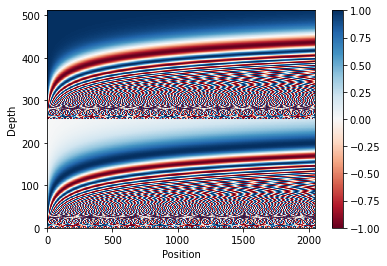
\includegraphics[width=0.5 \textwidth]{Chapters/2. Transformer/Figures/transformer/pos_enc.png}
    \caption{2000 Vectores de Positional Encoding con dimensiones de embedding=500.}
    \label{fig:trans_pos_enc}
\end{figure}

Poner una figura completa de todo el esquema del Transformer

\subsection{Problemas típicos en el entrenamiento de Transformers}

\subsubsection{Learning Rate WarmUp y Layer Normalization}

A pesar de que la arquitectura del modelo Transformer no es tan compleja, puesto que tanto el
codificador como el decodificador están formados por pilas de capas de atención y MLP, el
entrenamiento de este tipo de modelos muchas veces no resulta tan trivial. Regularmente requiere de
una combinación de técnicas para lograr su convergencia a valores aceptables y en conjunto con una
gran cantidad de datos, tamaños de lotes de procesamiento grandes y una gran cantidad de tiempo
de procesamiento en gpu \cite{DBLP:journals/corr/abs-1804-00247}.

\textit{Learning Rate WarmUp} es una de las primeras técnicas usadas y descritas en el proceso de
entrenamiento por \citeauthor{Vaswani}. Usando el algoritmo Adam como optimizador se varía el factor
de aprendizaje de acuerdo a la fórmula:

\begin{equation}
    lrate = d_{m}^{-0.5} \vdot \min\big(step\_num^{-0.5}, step\_num \vdot warmup\_steps^{-0.5} \big)
\end{equation}

En el esquema anterior, más conocido como \textit{Noam-Warmup}, el modelo original es entrenado
incrementando linealmente el factor de aprendizaje en los primeros $warmup\_steps=4000$ pasos.
Posteriormente, decrementa propocionalmente al inverso del la raíz cuadrada del paso $step\_num$
actual, véase la figura \ref{fig:noam}.

\begin{figure}[ht!]
    \centering
    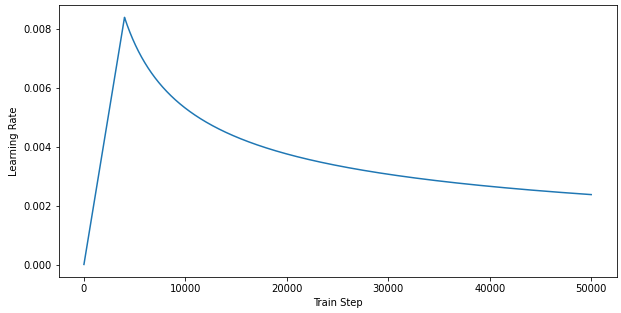
\includegraphics[width=0.5 \textwidth]{Chapters/2. Transformer/Figures/transformer/noam.png}
    \caption{Noam-Warmup con $warmup\_steps=4000$ y $d_{m} = 512$}
    \label{fig:noam}
\end{figure}

Si bien, la razón por la que funciona este tipo de técnica no está del todo claro, se presume que usar
\textit{Learning Rate WarmUp} ayuda a reducir la varianza del factor de aprendizaje adaptativo durante
las primeras etapas del entrenamiento del modelo. \citeauthor{DBLP:journals/corr/abs-1908-03265}
demostraron que el segundo momento del algoritmo
de Adam durante etapas tempranas de optimización es proporcional a una integral divergente, lo que
provoca las actualizaciones inestables, llevando al
modelo fuera de las regiones donde un mejor mínimo existe. Con esto en mente
\citeauthor{DBLP:journals/corr/abs-1908-03265} proponen el algoritmo de optimización
\textit{RAdam} (Rectified Adam) como una alternativa a usar \textit{Learning Rate WarmUp} y mitigar
este efecto durante la fase inicial del entrenamiento de los modelos.

El \textit{Learning Rate WarmUp}
comúnmente es usado en conjunto con algoritmos de optimización estocásticos como \textit{RMSprop} o
\textit{Adam}. En vez configurar el \textit{factor de aprendizaje} $\alpha$ con un decremento
constante, la estrategia de \textit{Learning Rate WarmUp} configura este factor con valores muy
pequeños en los primeros pasos de entrenamiento. Durante las primeras etapas del entrenamiento
el factor de aprendizaje es incrementado hasta un límite que es ligeramente superior o inferior al valor
inicial de $\alpha$ del optimizador usado y posteriormente es  decrementado
progresivamente hasta la convergencia del modelo.

Así, en cada paso del algoritmo de optimización el cuál está parametrizado por el factor de aprendizaje
$\alpha$, puede ser aplicado un factor de \textit{warmup} $\omega \in [0,1]$ que sirve para reducir
$\alpha$ y a la vez el paso de optimización en cada tiempo, replazando $\alpha_t = \alpha \omega_t$.
La forma mas sencilla es usar un factor \textbf{linear warmup} parametrizado por un periodo de
\quotes{calentamiento} $\tau$.

\begin{equation}
    \omega_t^{linear, \tau} = \min\big(1, \frac{t}{\tau} \big)
    \label{eq:warn_linear}
\end{equation}

\citeauthor{DBLP:journals/corr/abs-1910-04209} proponen 3 formas de aplicar la técnica de \textit{warmup}:

\textbf{Exponential warmup} aplica un decaimiento exponencial

\begin{equation}
    \omega_t^{expo, \tau} = 1 - \exp(- \frac{1}{\tau} t)
    \label{eq:warn_expo}
\end{equation}

recomienda elegir $\tau = (1 - \beta_2)^{-1}$ tal que no se tan diferente del segundo momento de
corrección de bias del algoritmo de \textit{Adam} $\beta_2$.

\begin{equation}
    \omega_t^{expo, untuned} = 1 - \exp(- (1 - \beta_2) t)
    \label{eq:warn_expo_untened}
\end{equation}

Similar al decaimiento exponencial proponen usar \textit{linear warmup} sobre
$\tau = 2 (1 - \beta_2)^{-1}$ iteraciones para preservar un efecto similar de des-aceleración
con el paso del tiempo.

\begin{equation}
    \omega_t^{linear, untuned} = \min\big(1, \frac{1 - \beta_2}{2} t \big)
    \label{eq:warn_linear_untuned}
\end{equation}

\begin{figure}[ht!]
    \centering
    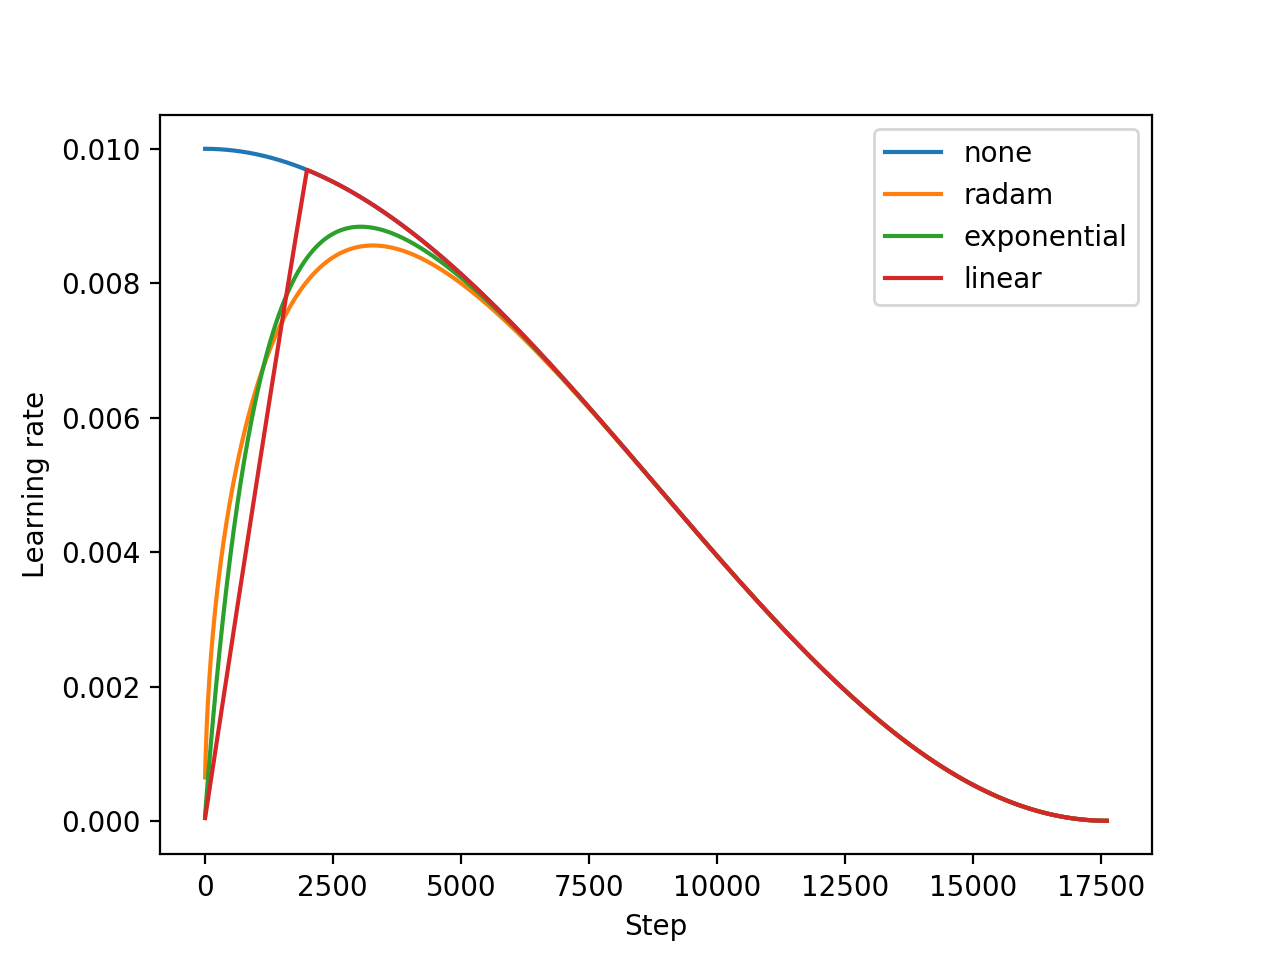
\includegraphics[width=0.5 \textwidth]{Chapters/2. Transformer/Figures/transformer/warmups.png}
    \caption{Learning rate sobre X 18000 iteraciones usando RAdam y lineal, exponencial warmup con Adam}
    \label{fig:warmup}
\end{figure}


Por otro lado, \citeauthor{pmlr-v119-huang20f} mencionan que usar la técnica de \textit{Learning Rate WarmUp}
para mitigar la varianza del optimizador Adam no es del todo la solución y que el problema radica
precisamente en la arquitectura del modelo Transformer, principalmente en las capas de normalización
\cite{DBLP:journals/corr/abs-1804-09849} \cite{DBLP:journals/corr/abs-2002-04745}. En particular
\citeauthor{DBLP:journals/corr/abs-2002-04745} encuentran que para un modelo Transformer de cualquier
tamaño con capas de normalización entre bloques residuales (\textit{Post-LN Transformer}), la escala
de la norma del gradiente que incide en la última capa de normalización permanecen igual al no depender
de la cantidad de bloques del transformer. Por el contrario, si la capa de normalización es colocada
justo antes de la conexión residual (\textit{Pre-LN Transformer}) la magnitud de la norma del
gradiente decrece conforme el tamaño del modelo incrementa, guiando así, al problema de desvanecimiento de
gradiente. \citeauthor{pmlr-v119-huang20f} proponen eliminar las capas de normalización del modelo
Transformer que en conjunto con la inestabilidad del algoritmo de optimización de Adam provocan la
dificultad de entrenamiento durante desde las primeras etapas. Para ello, estandarizan la siguiente
inicialización (\textit{T-Fixup}) de pesos del modelo, permitiendo evitar la etapa de \textit{WarmUp}
y las capas de normalización en el Transformer. La figura \ref{fig:t-fixup} muestra una comparativa
de los histogramas usando la inicialización \textit{T-Fixup} e usar el algoritmo de Adam con y sin
etapa de \textit{Warmup}:

\begin{itemize}
    \item Aplicar initialization tipo \textit{Xavier} para todos los pesos del modelo.
          Excepto el proceso de generación de embedding adecuados al tamaño del modelo $d_m$.
    \item Usar una inicialización tipo \textit{Gaussiana} con $\mathbb{N}(0, d_m^\frac{1}{2})$ para
          los pesos de generación de embeddings.
    \item Escalar las matrices $W_i^V$ y $W^O$ en cada bloque de atención en el decodificador, los
          pesos en de cada capa MLP del decodificador y los pesos de generación de embeddings tanto
          del codificador como decodificador por $9N^{-\frac{1}{4}}$ donde $N$ es el número de bloques
          del Transformer.
    \item Escalar las matrices $W_i^V$ y $W^O$ de cada bloque de atención del codificador y los pesos
          de cada capa de MLP del codificador por $0.67N^{-\frac{1}{4}}$
\end{itemize}

\begin{figure}[ht!]
    \centering
    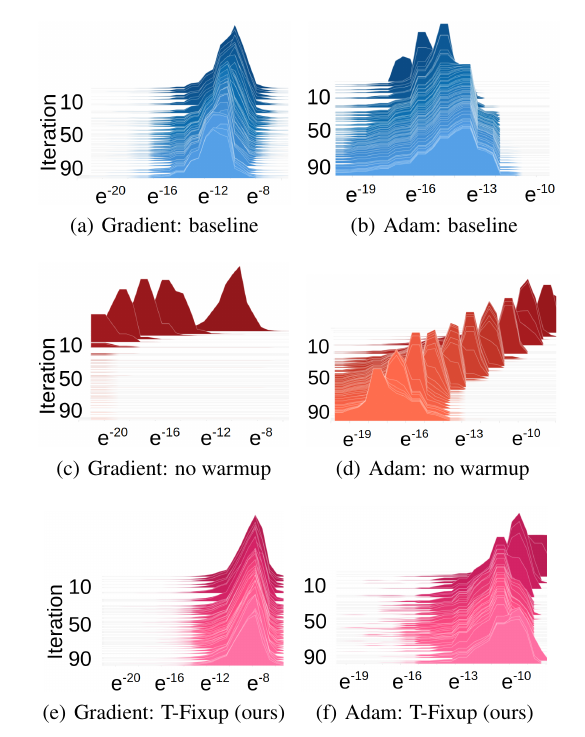
\includegraphics[width=0.5 \textwidth]{Chapters/2. Transformer/Figures/transformer/tfixup.png}
    \caption{Histograma de gradientes del Algoritmo Adam con y sin etapa de \textit{WarmUp} y
    usando inicialización \textit{T-Fixup}. Imagen original de \citeauthor{pmlr-v119-huang20f}}
    \label{fig:t-fixup}
\end{figure}

\subsubsection{Cálculo de la Atención}

Además de lo específico y delicado del entrenamiento del Modelo Transformer su costo en tiempo
computacional y de memoria también representa un serio problema a la hora de optimizar e inferir.
Debido principalmente a que en el proceso de atención debe focalizar cada token con respecto a todos
los demás, lo que lleva a que su complejidad crezca cuadráticamente con respecto a el tamaño de la
secuencia.

Varías técnicas han sido propuestas para reducir este problema, muchas de ellas involucran en reducir
la atención a vecindades de representaciones, aproximar la matriz de atención con otras matrices de
transformaciones a través de kernels o sustituir completamente la operación \textit{softmax}
por otra función.

\textbf{Atención de vecindades}:

\citeauthor{DBLP:journals/corr/abs-1802-05751} particionan la información de las representaciones de
las consultas asignándolos a diferentes bloques de memoria, restringiéndose a vecindarios locales
alrededor de cada consulta. Principalmente basados en cómo las redes convolucionales trabajar. Sin
embargo esta solucion es parcial y solo aplicable a secuencias de datos con relaciones cortas, cómo
imágenes.

\citeauthor{DBLP:journals/corr/abs-1904-10509} factorizan la matriz de atención para reducir su complejidad
de $O(n^2)$ a $O(n\sqrt(n))$ por medio de matrices ralas, separando la atención a través de diferentes
pasos al parametrizar la atención por una conectividad de distintos patrones elegidos previamente bajo el supuesto
de que las matrices de atención son ralas, puesto que no contienen dependencias de relevancia
sobre representaciones distantes como se observa en la imagen \ref{fig:att-spar}.

\begin{figure}[ht!]
    \centering
    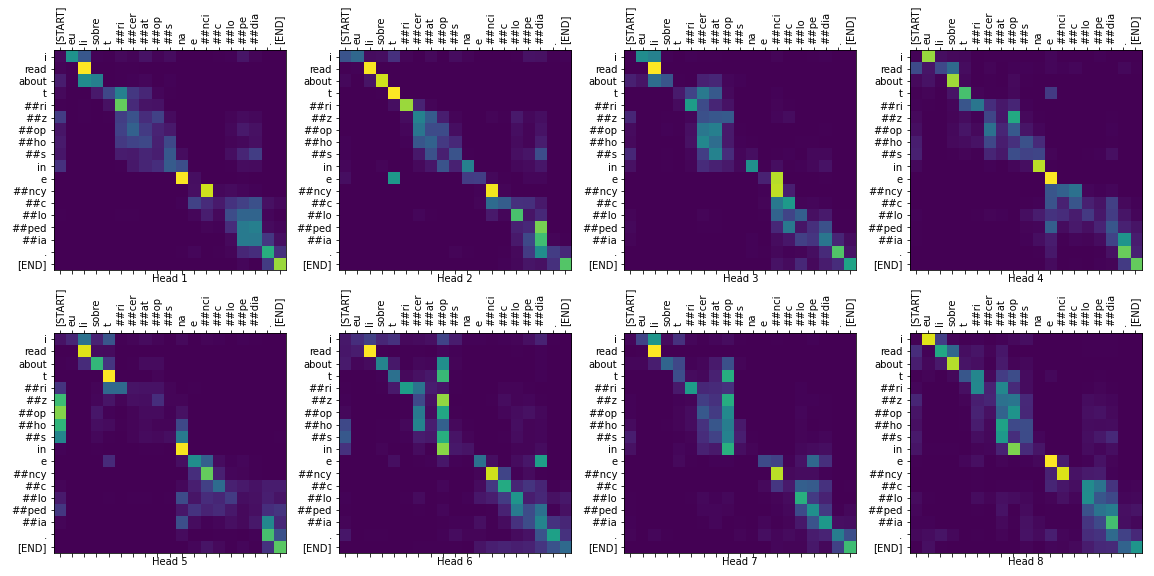
\includegraphics[width=0.7 \textwidth]{Chapters/2. Transformer/Figures/transformer/head_sparsity.png}
    \caption{Visualización de 8 cabezas de atención sobre una tarea de Machine-Translation. Las
    matrices de atención tienden a ser ralas al tener carencia de relaciones relevantes entre diversas
    representaciones a distancias lejanas.}
    \label{fig:att-spar}
\end{figure}

\citeauthor{DBLP:journals/corr/abs-1905-07799} proponen reducir el ancho de la atención basándose en
que cada representación no necesita prestar atención sobre todas las demás sino que debería ser
adaptativo. Así, para cada cabeza de atención se agrega una función de enmascaramiento que controla
la flexibilidad del ancho una ventana. La ventana formada cambia dinámicamente de tamaño
dependiendo de la representación en cuestión.
\citeauthor{DBLP:journals/corr/abs-2004-05150} siguen un estrategia similar, implementado
atención local con ventanas dilatadas distintas para cada cabeza, permitiendo atender contextos menos
locales en cada ocasión y atención global sobre preseleccionados localizaciones. Dada la dificultad de
su implementación sin usar ciclos para iterar sobre los elementos seleccionados a atender, implementan
su propio kernel en \textit{CUDA} con las operaciones optimizadas para realizar esta tarea.

\citeauthor{DBLP:journals/corr/abs-1901-02860} mencionan que si el problema es el procesamiento de
grandes secuencias por qué no dividirlas en secuencias más pequeñas y procesarlas individualmente
y así evitar usar grandes cantidades de memoria en su procesamiento. El principal problema de este
enfoque es que cada secuencia es procesada individualmente y la información de previas secuencias es
ignorada evitando que esta fluya a través de las próximas secuencias. Para solucionar este
inconveniente introducen un mecanismo de recurrencia en la arquitectura del transformer. Durante el
entrenamiento (véase la figura \ref{fig:trans-xl}) un estado oculto es calculado de las secuencias previas y guardado
en memoria para extender el contexto al momento de procesar la siguiente secuencia. Durante el
proceso de evaluación, el resultado de las operaciones del transformer pueden ser reusado y no
calculado nuevamente desde cero, permitiendo reducir considerablemente el tiempo de evaluación.

\begin{figure}[ht!]
    \centering
    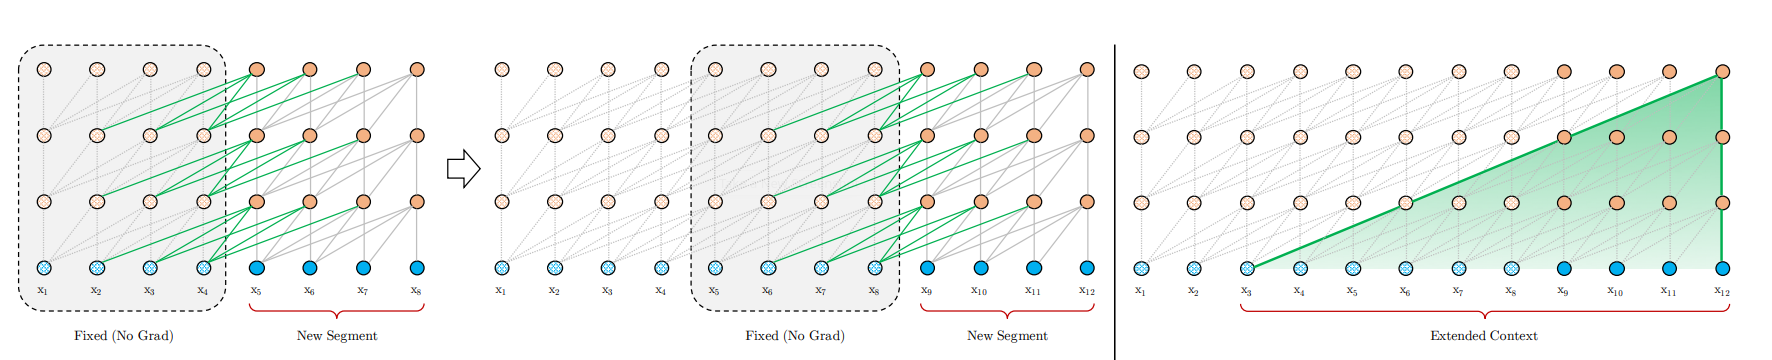
\includegraphics[width=0.8 \textwidth]{Chapters/2. Transformer/Figures/transformer/trans-XL.png}
    \caption{Transformer-XL. Para tratar con secuencias largas divide el proceso en secuencias más
             cortas creando estados ocultos intermedios y usandolos en el cálculo de las próximas
             secuencias. Figura obtenida de \cite{DBLP:journals/corr/abs-1901-02860}.}
    \label{fig:trans-xl}
\end{figure}

\citeauthor{DBLP:journals/corr/abs-2001-04451} reducen el problema de realizar la operación de softmax
sobre toda la matriz $Q_i K_i^\top$ a calcularlo individualmente por cada consulta $q_j$, guardando
solo una vez en memoria este valor en cada iteración y recalculándolo cuando se necesite de nuevo
al utilizar \textit{Back-Propagation} usando de capas reversibles. Si bien, computacionalmente es
más costoso permite usar mucho
menos memoria que la solución original. Por otro lado, dado que el resultado de la función softmax
depende en mucho mayor medida en los elementos dominantes de la matriz, solo es necesario fijarse en
las llaves más cercanas a la consulta en cuestión. \textit{LSH} (\textit{Local Sensitive Hashing})
resuelve este problema permitiendo encontrar rápidamente los vecinos más cercanos en espacios de altas
dimensiones, con la  restricción de que $W_i^Q = W_i^K$ dado que se necesita conservar la
similaridad entre consultas y llaves, algo que sería más dificil si sus matrices de proyección
$W_i^Q$ y $W_i^K$ fuesen muy distintas.

\textbf{Aproximaciones a la Atención original}:

También \citeauthor{DBLP:journals/corr/abs-1906-11024} proponen un modelo para compartir pesos de capas
adyacentes (Shared Attention Network - SAN).
Cada $\pi$ capas continuas en el codificador comparten la misma matriz de atención y en el
decodificador se comparte la proyección de los pesos de atención sobre la representación de los
valores $V_i$, en otras palabras se comparte directamente la cabeza de atención $head_i$. Dado que no
es tan fácil conocer que capas deben compartir pesos, establecen un proceso iterativo
de entrenamiento basados en calcular que tan diferentes son las capas del transformer usando
la \textit{Divergencia de Jensen-Shannon}. Si la similaridad entre dos capas es mayor a cierto umbral
se indica que dichas capas deben compartir pesos. Se repite un nuevo entrenamiento y se calcula
nuevamente la similaridad entre capas, y así sucesivamente hasta convergencia. Podemos notar que este
proceso de entrenamiento y ajuste de pesos es muy costoso, un nuevo entrenamiento es requerido por
cada ajuste de compartición de pesos, pero el modelo resultante
es menos complejo y el tiempo en modo de evaluación o inferencia se ve reducido considerablemente.

\citeauthor{DBLP:journals/corr/abs-2006-04768} bajo la hipótesis de que la matriz de atención tienen
rango mucho menor que $n$ proponen obtener los valores de cada cabeza haciendo una aproximación a ella.
Para ello, se hace uso de dos matrices entrenables conjuntamente con el modelo, $E$ y $F$
$\in \mathbb{R}^{n \times k}$ con $k \ll n$, tal que,
$head_i = softmax(\frac{Q_i (E_i K_i)}{\sqrt{d_m}}) F_iV_i$. Con ello la dimensión correspondiente al
tamaño de las secuencias se ve reducido bajo el supuesto que podemos representar la información
secuencial en un espacio más pequeño sin gran pérdida de información.

\citeauthor{DBLP:journals/corr/abs-2009-14794} por el contrario descomponen la operación de atención
sobre los valores $head = softmax(\frac{QK^\top}{\sqrt{d_k} V})$ en una multiplicación matricial más simple
$head = Q'k'^\top V$ con $Q'$ y $k'^\top \in \mathbb{R}^{n \times r}$ y $r<=n$.
Para ello construyen $Q'$ y $k'$ como dos matrices usando kernels tal que su producto forma una
aproximación a la función softmax aplicada al producto de $Q$ y $K$. Notemos que con ello podemos
reducir el costo computacional y en
memoria simplemente reduciendo el producto $Q'(k'^\top V)$ de derecha a izquierda.

Finalmente autores como \citeauthor{DBLP:journals/corr/abs-2105-03824} remplazan completamente
el bloque de \textit{Multihead Attention} con bloques que aplican operaciones de Transformada de
Fourier o lo largo de la dimensión de los  embeddings y de las secuencias. Probando que el usar
\textit{FFT} (Fast Fourier Transform) es suficiente para abstraer y modelar las relaciones. Y como
\citeauthor{DBLP:journals/corr/abs-2108-09084} que cambian la atención entre todas las consultas
y llaves por una sola con todas las llaves. Para esto, a través de atención sumarizan todos las
consultas en una consulta global. Este proceso es repetido con las llaves y valores como se observa
en la figura \ref{fig:fast-former}

\begin{figure}[ht!]
    \centering
    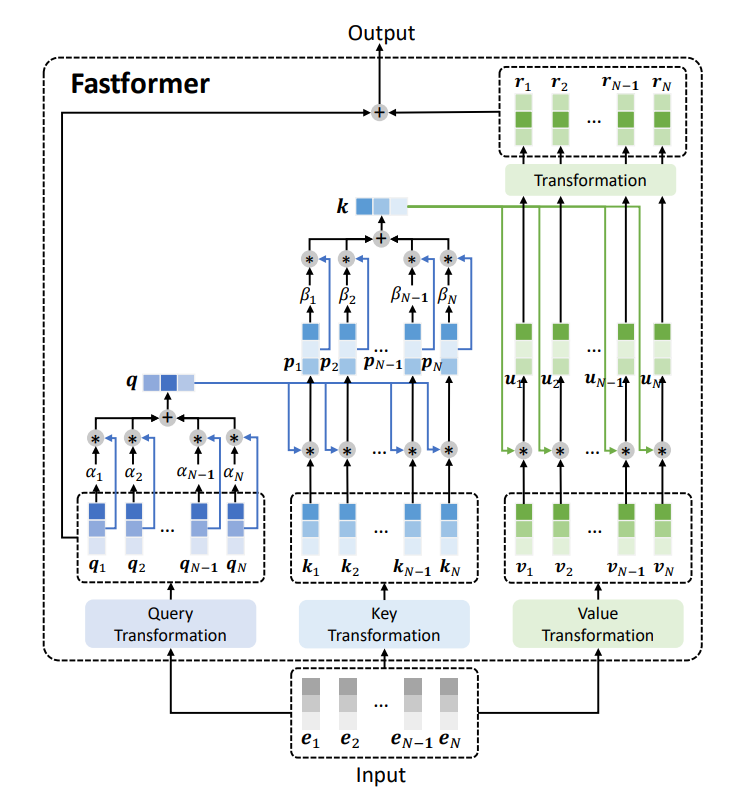
\includegraphics[width=0.6 \textwidth]{Chapters/2. Transformer/Figures/transformer/fastformer.png}
    \caption{Fast-Former. Remplaza la atención tradicional del  transformer por una iterativa. En
             cada paso crea una consulta y clave global usando atención sobre estos mismos.
             Figura obtenida de \cite{DBLP:journals/corr/abs-2108-09084}}
    \label{fig:fast-former}
\end{figure}


% \begin{figure}
%     \begin{center}
%         \scalebox{0.6}{%% Creator: Matplotlib, PGF backend
%%
%% To include the figure in your LaTeX document, write
%%   \input{<filename>.pgf}
%%
%% Make sure the required packages are loaded in your preamble
%%   \usepackage{pgf}
%%
%% Figures using additional raster images can only be included by \input if
%% they are in the same directory as the main LaTeX file. For loading figures
%% from other directories you can use the `import` package
%%   \usepackage{import}
%%
%% and then include the figures with
%%   \import{<path to file>}{<filename>.pgf}
%%
%% Matplotlib used the following preamble
%%
\begingroup%
\makeatletter%
\begin{pgfpicture}%
\pgfpathrectangle{\pgfpointorigin}{\pgfqpoint{10.000000in}{10.000000in}}%
\pgfusepath{use as bounding box, clip}%
\begin{pgfscope}%
\pgfsetbuttcap%
\pgfsetmiterjoin%
\pgfsetlinewidth{0.000000pt}%
\definecolor{currentstroke}{rgb}{1.000000,1.000000,1.000000}%
\pgfsetstrokecolor{currentstroke}%
\pgfsetstrokeopacity{0.000000}%
\pgfsetdash{}{0pt}%
\pgfpathmoveto{\pgfqpoint{0.000000in}{0.000000in}}%
\pgfpathlineto{\pgfqpoint{10.000000in}{0.000000in}}%
\pgfpathlineto{\pgfqpoint{10.000000in}{10.000000in}}%
\pgfpathlineto{\pgfqpoint{0.000000in}{10.000000in}}%
\pgfpathclose%
\pgfusepath{}%
\end{pgfscope}%
\begin{pgfscope}%
\pgfsetbuttcap%
\pgfsetmiterjoin%
\definecolor{currentfill}{rgb}{1.000000,1.000000,1.000000}%
\pgfsetfillcolor{currentfill}%
\pgfsetlinewidth{0.000000pt}%
\definecolor{currentstroke}{rgb}{0.000000,0.000000,0.000000}%
\pgfsetstrokecolor{currentstroke}%
\pgfsetstrokeopacity{0.000000}%
\pgfsetdash{}{0pt}%
\pgfpathmoveto{\pgfqpoint{0.763041in}{8.027083in}}%
\pgfpathlineto{\pgfqpoint{2.450346in}{8.027083in}}%
\pgfpathlineto{\pgfqpoint{2.450346in}{9.566628in}}%
\pgfpathlineto{\pgfqpoint{0.763041in}{9.566628in}}%
\pgfpathclose%
\pgfusepath{fill}%
\end{pgfscope}%
\begin{pgfscope}%
\pgfsetbuttcap%
\pgfsetroundjoin%
\definecolor{currentfill}{rgb}{0.000000,0.000000,0.000000}%
\pgfsetfillcolor{currentfill}%
\pgfsetlinewidth{0.803000pt}%
\definecolor{currentstroke}{rgb}{0.000000,0.000000,0.000000}%
\pgfsetstrokecolor{currentstroke}%
\pgfsetdash{}{0pt}%
\pgfsys@defobject{currentmarker}{\pgfqpoint{0.000000in}{-0.048611in}}{\pgfqpoint{0.000000in}{0.000000in}}{%
\pgfpathmoveto{\pgfqpoint{0.000000in}{0.000000in}}%
\pgfpathlineto{\pgfqpoint{0.000000in}{-0.048611in}}%
\pgfusepath{stroke,fill}%
}%
\begin{pgfscope}%
\pgfsys@transformshift{0.839736in}{8.027083in}%
\pgfsys@useobject{currentmarker}{}%
\end{pgfscope}%
\end{pgfscope}%
\begin{pgfscope}%
\definecolor{textcolor}{rgb}{0.000000,0.000000,0.000000}%
\pgfsetstrokecolor{textcolor}%
\pgfsetfillcolor{textcolor}%
\pgftext[x=0.839736in,y=7.929861in,,top]{\color{textcolor}\rmfamily\fontsize{10.000000}{12.000000}\selectfont \(\displaystyle {0.0}\)}%
\end{pgfscope}%
\begin{pgfscope}%
\pgfsetbuttcap%
\pgfsetroundjoin%
\definecolor{currentfill}{rgb}{0.000000,0.000000,0.000000}%
\pgfsetfillcolor{currentfill}%
\pgfsetlinewidth{0.803000pt}%
\definecolor{currentstroke}{rgb}{0.000000,0.000000,0.000000}%
\pgfsetstrokecolor{currentstroke}%
\pgfsetdash{}{0pt}%
\pgfsys@defobject{currentmarker}{\pgfqpoint{0.000000in}{-0.048611in}}{\pgfqpoint{0.000000in}{0.000000in}}{%
\pgfpathmoveto{\pgfqpoint{0.000000in}{0.000000in}}%
\pgfpathlineto{\pgfqpoint{0.000000in}{-0.048611in}}%
\pgfusepath{stroke,fill}%
}%
\begin{pgfscope}%
\pgfsys@transformshift{1.606693in}{8.027083in}%
\pgfsys@useobject{currentmarker}{}%
\end{pgfscope}%
\end{pgfscope}%
\begin{pgfscope}%
\definecolor{textcolor}{rgb}{0.000000,0.000000,0.000000}%
\pgfsetstrokecolor{textcolor}%
\pgfsetfillcolor{textcolor}%
\pgftext[x=1.606693in,y=7.929861in,,top]{\color{textcolor}\rmfamily\fontsize{10.000000}{12.000000}\selectfont \(\displaystyle {0.5}\)}%
\end{pgfscope}%
\begin{pgfscope}%
\pgfsetbuttcap%
\pgfsetroundjoin%
\definecolor{currentfill}{rgb}{0.000000,0.000000,0.000000}%
\pgfsetfillcolor{currentfill}%
\pgfsetlinewidth{0.803000pt}%
\definecolor{currentstroke}{rgb}{0.000000,0.000000,0.000000}%
\pgfsetstrokecolor{currentstroke}%
\pgfsetdash{}{0pt}%
\pgfsys@defobject{currentmarker}{\pgfqpoint{0.000000in}{-0.048611in}}{\pgfqpoint{0.000000in}{0.000000in}}{%
\pgfpathmoveto{\pgfqpoint{0.000000in}{0.000000in}}%
\pgfpathlineto{\pgfqpoint{0.000000in}{-0.048611in}}%
\pgfusepath{stroke,fill}%
}%
\begin{pgfscope}%
\pgfsys@transformshift{2.373650in}{8.027083in}%
\pgfsys@useobject{currentmarker}{}%
\end{pgfscope}%
\end{pgfscope}%
\begin{pgfscope}%
\definecolor{textcolor}{rgb}{0.000000,0.000000,0.000000}%
\pgfsetstrokecolor{textcolor}%
\pgfsetfillcolor{textcolor}%
\pgftext[x=2.373650in,y=7.929861in,,top]{\color{textcolor}\rmfamily\fontsize{10.000000}{12.000000}\selectfont \(\displaystyle {1.0}\)}%
\end{pgfscope}%
\begin{pgfscope}%
\definecolor{textcolor}{rgb}{0.000000,0.000000,0.000000}%
\pgfsetstrokecolor{textcolor}%
\pgfsetfillcolor{textcolor}%
\pgftext[x=1.606693in,y=7.750849in,,top]{\color{textcolor}\rmfamily\fontsize{16.000000}{19.200000}\selectfont FPR}%
\end{pgfscope}%
\begin{pgfscope}%
\pgfsetbuttcap%
\pgfsetroundjoin%
\definecolor{currentfill}{rgb}{0.000000,0.000000,0.000000}%
\pgfsetfillcolor{currentfill}%
\pgfsetlinewidth{0.803000pt}%
\definecolor{currentstroke}{rgb}{0.000000,0.000000,0.000000}%
\pgfsetstrokecolor{currentstroke}%
\pgfsetdash{}{0pt}%
\pgfsys@defobject{currentmarker}{\pgfqpoint{-0.048611in}{0.000000in}}{\pgfqpoint{-0.000000in}{0.000000in}}{%
\pgfpathmoveto{\pgfqpoint{-0.000000in}{0.000000in}}%
\pgfpathlineto{\pgfqpoint{-0.048611in}{0.000000in}}%
\pgfusepath{stroke,fill}%
}%
\begin{pgfscope}%
\pgfsys@transformshift{0.763041in}{8.097062in}%
\pgfsys@useobject{currentmarker}{}%
\end{pgfscope}%
\end{pgfscope}%
\begin{pgfscope}%
\definecolor{textcolor}{rgb}{0.000000,0.000000,0.000000}%
\pgfsetstrokecolor{textcolor}%
\pgfsetfillcolor{textcolor}%
\pgftext[x=0.418904in, y=8.048837in, left, base]{\color{textcolor}\rmfamily\fontsize{10.000000}{12.000000}\selectfont \(\displaystyle {0.00}\)}%
\end{pgfscope}%
\begin{pgfscope}%
\pgfsetbuttcap%
\pgfsetroundjoin%
\definecolor{currentfill}{rgb}{0.000000,0.000000,0.000000}%
\pgfsetfillcolor{currentfill}%
\pgfsetlinewidth{0.803000pt}%
\definecolor{currentstroke}{rgb}{0.000000,0.000000,0.000000}%
\pgfsetstrokecolor{currentstroke}%
\pgfsetdash{}{0pt}%
\pgfsys@defobject{currentmarker}{\pgfqpoint{-0.048611in}{0.000000in}}{\pgfqpoint{-0.000000in}{0.000000in}}{%
\pgfpathmoveto{\pgfqpoint{-0.000000in}{0.000000in}}%
\pgfpathlineto{\pgfqpoint{-0.048611in}{0.000000in}}%
\pgfusepath{stroke,fill}%
}%
\begin{pgfscope}%
\pgfsys@transformshift{0.763041in}{8.446959in}%
\pgfsys@useobject{currentmarker}{}%
\end{pgfscope}%
\end{pgfscope}%
\begin{pgfscope}%
\definecolor{textcolor}{rgb}{0.000000,0.000000,0.000000}%
\pgfsetstrokecolor{textcolor}%
\pgfsetfillcolor{textcolor}%
\pgftext[x=0.418904in, y=8.398734in, left, base]{\color{textcolor}\rmfamily\fontsize{10.000000}{12.000000}\selectfont \(\displaystyle {0.25}\)}%
\end{pgfscope}%
\begin{pgfscope}%
\pgfsetbuttcap%
\pgfsetroundjoin%
\definecolor{currentfill}{rgb}{0.000000,0.000000,0.000000}%
\pgfsetfillcolor{currentfill}%
\pgfsetlinewidth{0.803000pt}%
\definecolor{currentstroke}{rgb}{0.000000,0.000000,0.000000}%
\pgfsetstrokecolor{currentstroke}%
\pgfsetdash{}{0pt}%
\pgfsys@defobject{currentmarker}{\pgfqpoint{-0.048611in}{0.000000in}}{\pgfqpoint{-0.000000in}{0.000000in}}{%
\pgfpathmoveto{\pgfqpoint{-0.000000in}{0.000000in}}%
\pgfpathlineto{\pgfqpoint{-0.048611in}{0.000000in}}%
\pgfusepath{stroke,fill}%
}%
\begin{pgfscope}%
\pgfsys@transformshift{0.763041in}{8.796856in}%
\pgfsys@useobject{currentmarker}{}%
\end{pgfscope}%
\end{pgfscope}%
\begin{pgfscope}%
\definecolor{textcolor}{rgb}{0.000000,0.000000,0.000000}%
\pgfsetstrokecolor{textcolor}%
\pgfsetfillcolor{textcolor}%
\pgftext[x=0.418904in, y=8.748630in, left, base]{\color{textcolor}\rmfamily\fontsize{10.000000}{12.000000}\selectfont \(\displaystyle {0.50}\)}%
\end{pgfscope}%
\begin{pgfscope}%
\pgfsetbuttcap%
\pgfsetroundjoin%
\definecolor{currentfill}{rgb}{0.000000,0.000000,0.000000}%
\pgfsetfillcolor{currentfill}%
\pgfsetlinewidth{0.803000pt}%
\definecolor{currentstroke}{rgb}{0.000000,0.000000,0.000000}%
\pgfsetstrokecolor{currentstroke}%
\pgfsetdash{}{0pt}%
\pgfsys@defobject{currentmarker}{\pgfqpoint{-0.048611in}{0.000000in}}{\pgfqpoint{-0.000000in}{0.000000in}}{%
\pgfpathmoveto{\pgfqpoint{-0.000000in}{0.000000in}}%
\pgfpathlineto{\pgfqpoint{-0.048611in}{0.000000in}}%
\pgfusepath{stroke,fill}%
}%
\begin{pgfscope}%
\pgfsys@transformshift{0.763041in}{9.146752in}%
\pgfsys@useobject{currentmarker}{}%
\end{pgfscope}%
\end{pgfscope}%
\begin{pgfscope}%
\definecolor{textcolor}{rgb}{0.000000,0.000000,0.000000}%
\pgfsetstrokecolor{textcolor}%
\pgfsetfillcolor{textcolor}%
\pgftext[x=0.418904in, y=9.098527in, left, base]{\color{textcolor}\rmfamily\fontsize{10.000000}{12.000000}\selectfont \(\displaystyle {0.75}\)}%
\end{pgfscope}%
\begin{pgfscope}%
\pgfsetbuttcap%
\pgfsetroundjoin%
\definecolor{currentfill}{rgb}{0.000000,0.000000,0.000000}%
\pgfsetfillcolor{currentfill}%
\pgfsetlinewidth{0.803000pt}%
\definecolor{currentstroke}{rgb}{0.000000,0.000000,0.000000}%
\pgfsetstrokecolor{currentstroke}%
\pgfsetdash{}{0pt}%
\pgfsys@defobject{currentmarker}{\pgfqpoint{-0.048611in}{0.000000in}}{\pgfqpoint{-0.000000in}{0.000000in}}{%
\pgfpathmoveto{\pgfqpoint{-0.000000in}{0.000000in}}%
\pgfpathlineto{\pgfqpoint{-0.048611in}{0.000000in}}%
\pgfusepath{stroke,fill}%
}%
\begin{pgfscope}%
\pgfsys@transformshift{0.763041in}{9.496649in}%
\pgfsys@useobject{currentmarker}{}%
\end{pgfscope}%
\end{pgfscope}%
\begin{pgfscope}%
\definecolor{textcolor}{rgb}{0.000000,0.000000,0.000000}%
\pgfsetstrokecolor{textcolor}%
\pgfsetfillcolor{textcolor}%
\pgftext[x=0.418904in, y=9.448424in, left, base]{\color{textcolor}\rmfamily\fontsize{10.000000}{12.000000}\selectfont \(\displaystyle {1.00}\)}%
\end{pgfscope}%
\begin{pgfscope}%
\definecolor{textcolor}{rgb}{0.000000,0.000000,0.000000}%
\pgfsetstrokecolor{textcolor}%
\pgfsetfillcolor{textcolor}%
\pgftext[x=0.363349in,y=8.796856in,,bottom,rotate=90.000000]{\color{textcolor}\rmfamily\fontsize{16.000000}{19.200000}\selectfont TPR}%
\end{pgfscope}%
\begin{pgfscope}%
\pgfpathrectangle{\pgfqpoint{0.763041in}{8.027083in}}{\pgfqpoint{1.687305in}{1.539545in}}%
\pgfusepath{clip}%
\pgfsetrectcap%
\pgfsetroundjoin%
\pgfsetlinewidth{1.505625pt}%
\definecolor{currentstroke}{rgb}{0.000000,0.501961,0.000000}%
\pgfsetstrokecolor{currentstroke}%
\pgfsetdash{}{0pt}%
\pgfpathmoveto{\pgfqpoint{0.839736in}{8.097062in}}%
\pgfpathlineto{\pgfqpoint{0.839795in}{8.097062in}}%
\pgfpathlineto{\pgfqpoint{0.839795in}{8.098372in}}%
\pgfpathlineto{\pgfqpoint{0.842028in}{8.174308in}}%
\pgfpathlineto{\pgfqpoint{0.843556in}{8.205730in}}%
\pgfpathlineto{\pgfqpoint{0.843614in}{8.205730in}}%
\pgfpathlineto{\pgfqpoint{0.845142in}{8.237152in}}%
\pgfpathlineto{\pgfqpoint{0.845436in}{8.238461in}}%
\pgfpathlineto{\pgfqpoint{0.846435in}{8.255481in}}%
\pgfpathlineto{\pgfqpoint{0.847022in}{8.255481in}}%
\pgfpathlineto{\pgfqpoint{0.848491in}{8.286903in}}%
\pgfpathlineto{\pgfqpoint{0.848785in}{8.288213in}}%
\pgfpathlineto{\pgfqpoint{0.850195in}{8.315707in}}%
\pgfpathlineto{\pgfqpoint{0.850900in}{8.317016in}}%
\pgfpathlineto{\pgfqpoint{0.852310in}{8.337964in}}%
\pgfpathlineto{\pgfqpoint{0.852839in}{8.339273in}}%
\pgfpathlineto{\pgfqpoint{0.854308in}{8.365458in}}%
\pgfpathlineto{\pgfqpoint{0.854602in}{8.366768in}}%
\pgfpathlineto{\pgfqpoint{0.856071in}{8.391643in}}%
\pgfpathlineto{\pgfqpoint{0.856365in}{8.392953in}}%
\pgfpathlineto{\pgfqpoint{0.857892in}{8.413900in}}%
\pgfpathlineto{\pgfqpoint{0.858069in}{8.415210in}}%
\pgfpathlineto{\pgfqpoint{0.859596in}{8.441395in}}%
\pgfpathlineto{\pgfqpoint{0.859714in}{8.441395in}}%
\pgfpathlineto{\pgfqpoint{0.861183in}{8.461033in}}%
\pgfpathlineto{\pgfqpoint{0.861359in}{8.461033in}}%
\pgfpathlineto{\pgfqpoint{0.862417in}{8.478054in}}%
\pgfpathlineto{\pgfqpoint{0.863592in}{8.479363in}}%
\pgfpathlineto{\pgfqpoint{0.865061in}{8.487218in}}%
\pgfpathlineto{\pgfqpoint{0.865707in}{8.488528in}}%
\pgfpathlineto{\pgfqpoint{0.867176in}{8.501620in}}%
\pgfpathlineto{\pgfqpoint{0.867293in}{8.501620in}}%
\pgfpathlineto{\pgfqpoint{0.868704in}{8.522568in}}%
\pgfpathlineto{\pgfqpoint{0.868880in}{8.522568in}}%
\pgfpathlineto{\pgfqpoint{0.869996in}{8.534351in}}%
\pgfpathlineto{\pgfqpoint{0.870878in}{8.534351in}}%
\pgfpathlineto{\pgfqpoint{0.872229in}{8.551372in}}%
\pgfpathlineto{\pgfqpoint{0.872464in}{8.551372in}}%
\pgfpathlineto{\pgfqpoint{0.873933in}{8.567083in}}%
\pgfpathlineto{\pgfqpoint{0.874051in}{8.567083in}}%
\pgfpathlineto{\pgfqpoint{0.875578in}{8.576247in}}%
\pgfpathlineto{\pgfqpoint{0.875990in}{8.577557in}}%
\pgfpathlineto{\pgfqpoint{0.877517in}{8.593268in}}%
\pgfpathlineto{\pgfqpoint{0.877576in}{8.593268in}}%
\pgfpathlineto{\pgfqpoint{0.878869in}{8.611597in}}%
\pgfpathlineto{\pgfqpoint{0.879985in}{8.612906in}}%
\pgfpathlineto{\pgfqpoint{0.881513in}{8.627308in}}%
\pgfpathlineto{\pgfqpoint{0.881689in}{8.628617in}}%
\pgfpathlineto{\pgfqpoint{0.882512in}{8.637782in}}%
\pgfpathlineto{\pgfqpoint{0.883334in}{8.637782in}}%
\pgfpathlineto{\pgfqpoint{0.884744in}{8.650874in}}%
\pgfpathlineto{\pgfqpoint{0.884979in}{8.650874in}}%
\pgfpathlineto{\pgfqpoint{0.886507in}{8.662658in}}%
\pgfpathlineto{\pgfqpoint{0.887153in}{8.663967in}}%
\pgfpathlineto{\pgfqpoint{0.888564in}{8.677059in}}%
\pgfpathlineto{\pgfqpoint{0.888975in}{8.678369in}}%
\pgfpathlineto{\pgfqpoint{0.890150in}{8.691461in}}%
\pgfpathlineto{\pgfqpoint{0.891325in}{8.692770in}}%
\pgfpathlineto{\pgfqpoint{0.892265in}{8.707172in}}%
\pgfpathlineto{\pgfqpoint{0.893617in}{8.708481in}}%
\pgfpathlineto{\pgfqpoint{0.894909in}{8.717646in}}%
\pgfpathlineto{\pgfqpoint{0.895321in}{8.718955in}}%
\pgfpathlineto{\pgfqpoint{0.896848in}{8.732048in}}%
\pgfpathlineto{\pgfqpoint{0.897495in}{8.733357in}}%
\pgfpathlineto{\pgfqpoint{0.898964in}{8.743831in}}%
\pgfpathlineto{\pgfqpoint{0.899316in}{8.745140in}}%
\pgfpathlineto{\pgfqpoint{0.900668in}{8.751687in}}%
\pgfpathlineto{\pgfqpoint{0.902019in}{8.752996in}}%
\pgfpathlineto{\pgfqpoint{0.903370in}{8.766088in}}%
\pgfpathlineto{\pgfqpoint{0.904193in}{8.767398in}}%
\pgfpathlineto{\pgfqpoint{0.905721in}{8.772635in}}%
\pgfpathlineto{\pgfqpoint{0.905897in}{8.773944in}}%
\pgfpathlineto{\pgfqpoint{0.906661in}{8.781799in}}%
\pgfpathlineto{\pgfqpoint{0.907718in}{8.783109in}}%
\pgfpathlineto{\pgfqpoint{0.909187in}{8.793583in}}%
\pgfpathlineto{\pgfqpoint{0.909599in}{8.793583in}}%
\pgfpathlineto{\pgfqpoint{0.910833in}{8.806675in}}%
\pgfpathlineto{\pgfqpoint{0.911949in}{8.807984in}}%
\pgfpathlineto{\pgfqpoint{0.912713in}{8.817149in}}%
\pgfpathlineto{\pgfqpoint{0.914711in}{8.818458in}}%
\pgfpathlineto{\pgfqpoint{0.915827in}{8.822386in}}%
\pgfpathlineto{\pgfqpoint{0.917120in}{8.823695in}}%
\pgfpathlineto{\pgfqpoint{0.918177in}{8.827623in}}%
\pgfpathlineto{\pgfqpoint{0.919470in}{8.828932in}}%
\pgfpathlineto{\pgfqpoint{0.919470in}{8.830241in}}%
\pgfpathlineto{\pgfqpoint{0.921526in}{8.831551in}}%
\pgfpathlineto{\pgfqpoint{0.922760in}{8.836788in}}%
\pgfpathlineto{\pgfqpoint{0.923759in}{8.838097in}}%
\pgfpathlineto{\pgfqpoint{0.925052in}{8.847262in}}%
\pgfpathlineto{\pgfqpoint{0.926344in}{8.848571in}}%
\pgfpathlineto{\pgfqpoint{0.927872in}{8.851189in}}%
\pgfpathlineto{\pgfqpoint{0.929517in}{8.852499in}}%
\pgfpathlineto{\pgfqpoint{0.931045in}{8.856426in}}%
\pgfpathlineto{\pgfqpoint{0.931221in}{8.857736in}}%
\pgfpathlineto{\pgfqpoint{0.932573in}{8.865591in}}%
\pgfpathlineto{\pgfqpoint{0.933865in}{8.866900in}}%
\pgfpathlineto{\pgfqpoint{0.935217in}{8.877374in}}%
\pgfpathlineto{\pgfqpoint{0.938683in}{8.878684in}}%
\pgfpathlineto{\pgfqpoint{0.940211in}{8.882611in}}%
\pgfpathlineto{\pgfqpoint{0.940387in}{8.883921in}}%
\pgfpathlineto{\pgfqpoint{0.941915in}{8.891776in}}%
\pgfpathlineto{\pgfqpoint{0.942738in}{8.893085in}}%
\pgfpathlineto{\pgfqpoint{0.943384in}{8.897013in}}%
\pgfpathlineto{\pgfqpoint{0.945088in}{8.898322in}}%
\pgfpathlineto{\pgfqpoint{0.946616in}{8.902250in}}%
\pgfpathlineto{\pgfqpoint{0.947556in}{8.903559in}}%
\pgfpathlineto{\pgfqpoint{0.949025in}{8.914033in}}%
\pgfpathlineto{\pgfqpoint{0.949906in}{8.915343in}}%
\pgfpathlineto{\pgfqpoint{0.950846in}{8.919270in}}%
\pgfpathlineto{\pgfqpoint{0.953314in}{8.920580in}}%
\pgfpathlineto{\pgfqpoint{0.954313in}{8.925817in}}%
\pgfpathlineto{\pgfqpoint{0.956076in}{8.927126in}}%
\pgfpathlineto{\pgfqpoint{0.957603in}{8.934981in}}%
\pgfpathlineto{\pgfqpoint{0.958132in}{8.936291in}}%
\pgfpathlineto{\pgfqpoint{0.959307in}{8.941528in}}%
\pgfpathlineto{\pgfqpoint{0.960482in}{8.942837in}}%
\pgfpathlineto{\pgfqpoint{0.961305in}{8.945455in}}%
\pgfpathlineto{\pgfqpoint{0.962598in}{8.946765in}}%
\pgfpathlineto{\pgfqpoint{0.963655in}{8.950692in}}%
\pgfpathlineto{\pgfqpoint{0.965300in}{8.952002in}}%
\pgfpathlineto{\pgfqpoint{0.966769in}{8.955929in}}%
\pgfpathlineto{\pgfqpoint{0.967357in}{8.957239in}}%
\pgfpathlineto{\pgfqpoint{0.968826in}{8.962476in}}%
\pgfpathlineto{\pgfqpoint{0.969942in}{8.962476in}}%
\pgfpathlineto{\pgfqpoint{0.970295in}{8.966403in}}%
\pgfpathlineto{\pgfqpoint{0.971705in}{8.967713in}}%
\pgfpathlineto{\pgfqpoint{0.972880in}{8.971640in}}%
\pgfpathlineto{\pgfqpoint{0.974114in}{8.972950in}}%
\pgfpathlineto{\pgfqpoint{0.975230in}{8.976877in}}%
\pgfpathlineto{\pgfqpoint{0.976170in}{8.978187in}}%
\pgfpathlineto{\pgfqpoint{0.977522in}{8.982114in}}%
\pgfpathlineto{\pgfqpoint{0.979872in}{8.983424in}}%
\pgfpathlineto{\pgfqpoint{0.981047in}{8.989970in}}%
\pgfpathlineto{\pgfqpoint{0.983398in}{8.991279in}}%
\pgfpathlineto{\pgfqpoint{0.984925in}{8.996516in}}%
\pgfpathlineto{\pgfqpoint{0.985924in}{8.997825in}}%
\pgfpathlineto{\pgfqpoint{0.986394in}{9.004371in}}%
\pgfpathlineto{\pgfqpoint{0.988509in}{9.004371in}}%
\pgfpathlineto{\pgfqpoint{0.989920in}{9.013536in}}%
\pgfpathlineto{\pgfqpoint{0.990977in}{9.014845in}}%
\pgfpathlineto{\pgfqpoint{0.991506in}{9.018773in}}%
\pgfpathlineto{\pgfqpoint{0.994973in}{9.020082in}}%
\pgfpathlineto{\pgfqpoint{0.996265in}{9.022701in}}%
\pgfpathlineto{\pgfqpoint{0.997617in}{9.024010in}}%
\pgfpathlineto{\pgfqpoint{0.998851in}{9.027938in}}%
\pgfpathlineto{\pgfqpoint{1.002024in}{9.029247in}}%
\pgfpathlineto{\pgfqpoint{1.002024in}{9.030556in}}%
\pgfpathlineto{\pgfqpoint{1.004315in}{9.031866in}}%
\pgfpathlineto{\pgfqpoint{1.005667in}{9.038412in}}%
\pgfpathlineto{\pgfqpoint{1.007547in}{9.039721in}}%
\pgfpathlineto{\pgfqpoint{1.007547in}{9.041030in}}%
\pgfpathlineto{\pgfqpoint{1.010661in}{9.042340in}}%
\pgfpathlineto{\pgfqpoint{1.011836in}{9.046267in}}%
\pgfpathlineto{\pgfqpoint{1.012541in}{9.047577in}}%
\pgfpathlineto{\pgfqpoint{1.014010in}{9.054123in}}%
\pgfpathlineto{\pgfqpoint{1.014715in}{9.055432in}}%
\pgfpathlineto{\pgfqpoint{1.015362in}{9.060669in}}%
\pgfpathlineto{\pgfqpoint{1.019063in}{9.061978in}}%
\pgfpathlineto{\pgfqpoint{1.019710in}{9.064597in}}%
\pgfpathlineto{\pgfqpoint{1.022295in}{9.065906in}}%
\pgfpathlineto{\pgfqpoint{1.022295in}{9.067215in}}%
\pgfpathlineto{\pgfqpoint{1.026408in}{9.068525in}}%
\pgfpathlineto{\pgfqpoint{1.026408in}{9.069834in}}%
\pgfpathlineto{\pgfqpoint{1.031285in}{9.071143in}}%
\pgfpathlineto{\pgfqpoint{1.032812in}{9.077689in}}%
\pgfpathlineto{\pgfqpoint{1.036808in}{9.078999in}}%
\pgfpathlineto{\pgfqpoint{1.037924in}{9.084236in}}%
\pgfpathlineto{\pgfqpoint{1.040803in}{9.085545in}}%
\pgfpathlineto{\pgfqpoint{1.041743in}{9.090782in}}%
\pgfpathlineto{\pgfqpoint{1.042684in}{9.090782in}}%
\pgfpathlineto{\pgfqpoint{1.043212in}{9.096019in}}%
\pgfpathlineto{\pgfqpoint{1.053730in}{9.097328in}}%
\pgfpathlineto{\pgfqpoint{1.053730in}{9.098637in}}%
\pgfpathlineto{\pgfqpoint{1.057197in}{9.099947in}}%
\pgfpathlineto{\pgfqpoint{1.057608in}{9.102565in}}%
\pgfpathlineto{\pgfqpoint{1.061427in}{9.103874in}}%
\pgfpathlineto{\pgfqpoint{1.061897in}{9.107802in}}%
\pgfpathlineto{\pgfqpoint{1.065540in}{9.109111in}}%
\pgfpathlineto{\pgfqpoint{1.066950in}{9.113039in}}%
\pgfpathlineto{\pgfqpoint{1.068008in}{9.113039in}}%
\pgfpathlineto{\pgfqpoint{1.068478in}{9.118276in}}%
\pgfpathlineto{\pgfqpoint{1.072238in}{9.119585in}}%
\pgfpathlineto{\pgfqpoint{1.072238in}{9.120895in}}%
\pgfpathlineto{\pgfqpoint{1.074824in}{9.122204in}}%
\pgfpathlineto{\pgfqpoint{1.075411in}{9.124822in}}%
\pgfpathlineto{\pgfqpoint{1.077762in}{9.126132in}}%
\pgfpathlineto{\pgfqpoint{1.077762in}{9.127441in}}%
\pgfpathlineto{\pgfqpoint{1.081933in}{9.128750in}}%
\pgfpathlineto{\pgfqpoint{1.082462in}{9.131369in}}%
\pgfpathlineto{\pgfqpoint{1.092392in}{9.132678in}}%
\pgfpathlineto{\pgfqpoint{1.093861in}{9.136606in}}%
\pgfpathlineto{\pgfqpoint{1.097093in}{9.137915in}}%
\pgfpathlineto{\pgfqpoint{1.098092in}{9.141843in}}%
\pgfpathlineto{\pgfqpoint{1.100677in}{9.143152in}}%
\pgfpathlineto{\pgfqpoint{1.101676in}{9.145770in}}%
\pgfpathlineto{\pgfqpoint{1.103673in}{9.147080in}}%
\pgfpathlineto{\pgfqpoint{1.103673in}{9.148389in}}%
\pgfpathlineto{\pgfqpoint{1.108433in}{9.149698in}}%
\pgfpathlineto{\pgfqpoint{1.109608in}{9.153626in}}%
\pgfpathlineto{\pgfqpoint{1.111371in}{9.154935in}}%
\pgfpathlineto{\pgfqpoint{1.112017in}{9.157554in}}%
\pgfpathlineto{\pgfqpoint{1.115131in}{9.158863in}}%
\pgfpathlineto{\pgfqpoint{1.116600in}{9.162791in}}%
\pgfpathlineto{\pgfqpoint{1.117951in}{9.164100in}}%
\pgfpathlineto{\pgfqpoint{1.117951in}{9.165409in}}%
\pgfpathlineto{\pgfqpoint{1.124297in}{9.166718in}}%
\pgfpathlineto{\pgfqpoint{1.124885in}{9.169337in}}%
\pgfpathlineto{\pgfqpoint{1.131289in}{9.170646in}}%
\pgfpathlineto{\pgfqpoint{1.131289in}{9.171955in}}%
\pgfpathlineto{\pgfqpoint{1.135226in}{9.173265in}}%
\pgfpathlineto{\pgfqpoint{1.135520in}{9.177192in}}%
\pgfpathlineto{\pgfqpoint{1.138634in}{9.178502in}}%
\pgfpathlineto{\pgfqpoint{1.138634in}{9.179811in}}%
\pgfpathlineto{\pgfqpoint{1.141337in}{9.181120in}}%
\pgfpathlineto{\pgfqpoint{1.141337in}{9.182429in}}%
\pgfpathlineto{\pgfqpoint{1.152207in}{9.183739in}}%
\pgfpathlineto{\pgfqpoint{1.152559in}{9.186357in}}%
\pgfpathlineto{\pgfqpoint{1.156966in}{9.187666in}}%
\pgfpathlineto{\pgfqpoint{1.157906in}{9.190285in}}%
\pgfpathlineto{\pgfqpoint{1.160139in}{9.191594in}}%
\pgfpathlineto{\pgfqpoint{1.161020in}{9.195522in}}%
\pgfpathlineto{\pgfqpoint{1.167307in}{9.196831in}}%
\pgfpathlineto{\pgfqpoint{1.168776in}{9.202068in}}%
\pgfpathlineto{\pgfqpoint{1.170480in}{9.203377in}}%
\pgfpathlineto{\pgfqpoint{1.171714in}{9.207305in}}%
\pgfpathlineto{\pgfqpoint{1.174358in}{9.208614in}}%
\pgfpathlineto{\pgfqpoint{1.174593in}{9.211233in}}%
\pgfpathlineto{\pgfqpoint{1.177531in}{9.212542in}}%
\pgfpathlineto{\pgfqpoint{1.178765in}{9.216470in}}%
\pgfpathlineto{\pgfqpoint{1.186991in}{9.217779in}}%
\pgfpathlineto{\pgfqpoint{1.186991in}{9.219088in}}%
\pgfpathlineto{\pgfqpoint{1.193161in}{9.220397in}}%
\pgfpathlineto{\pgfqpoint{1.193983in}{9.223016in}}%
\pgfpathlineto{\pgfqpoint{1.198801in}{9.224325in}}%
\pgfpathlineto{\pgfqpoint{1.199800in}{9.228253in}}%
\pgfpathlineto{\pgfqpoint{1.202856in}{9.228253in}}%
\pgfpathlineto{\pgfqpoint{1.204148in}{9.232181in}}%
\pgfpathlineto{\pgfqpoint{1.205735in}{9.233490in}}%
\pgfpathlineto{\pgfqpoint{1.206087in}{9.236108in}}%
\pgfpathlineto{\pgfqpoint{1.209084in}{9.237418in}}%
\pgfpathlineto{\pgfqpoint{1.209084in}{9.238727in}}%
\pgfpathlineto{\pgfqpoint{1.213961in}{9.240036in}}%
\pgfpathlineto{\pgfqpoint{1.214313in}{9.242655in}}%
\pgfpathlineto{\pgfqpoint{1.218779in}{9.243964in}}%
\pgfpathlineto{\pgfqpoint{1.219895in}{9.246582in}}%
\pgfpathlineto{\pgfqpoint{1.221658in}{9.246582in}}%
\pgfpathlineto{\pgfqpoint{1.222892in}{9.253129in}}%
\pgfpathlineto{\pgfqpoint{1.227827in}{9.254438in}}%
\pgfpathlineto{\pgfqpoint{1.228826in}{9.257056in}}%
\pgfpathlineto{\pgfqpoint{1.234232in}{9.258366in}}%
\pgfpathlineto{\pgfqpoint{1.234232in}{9.259675in}}%
\pgfpathlineto{\pgfqpoint{1.237699in}{9.260984in}}%
\pgfpathlineto{\pgfqpoint{1.239109in}{9.263603in}}%
\pgfpathlineto{\pgfqpoint{1.241870in}{9.264912in}}%
\pgfpathlineto{\pgfqpoint{1.242987in}{9.267530in}}%
\pgfpathlineto{\pgfqpoint{1.246688in}{9.268840in}}%
\pgfpathlineto{\pgfqpoint{1.246688in}{9.270149in}}%
\pgfpathlineto{\pgfqpoint{1.260261in}{9.271458in}}%
\pgfpathlineto{\pgfqpoint{1.261789in}{9.274077in}}%
\pgfpathlineto{\pgfqpoint{1.271131in}{9.275386in}}%
\pgfpathlineto{\pgfqpoint{1.271131in}{9.276695in}}%
\pgfpathlineto{\pgfqpoint{1.275832in}{9.278004in}}%
\pgfpathlineto{\pgfqpoint{1.275832in}{9.279314in}}%
\pgfpathlineto{\pgfqpoint{1.281473in}{9.280623in}}%
\pgfpathlineto{\pgfqpoint{1.282765in}{9.283241in}}%
\pgfpathlineto{\pgfqpoint{1.285409in}{9.284551in}}%
\pgfpathlineto{\pgfqpoint{1.285409in}{9.285860in}}%
\pgfpathlineto{\pgfqpoint{1.292519in}{9.287169in}}%
\pgfpathlineto{\pgfqpoint{1.292519in}{9.288478in}}%
\pgfpathlineto{\pgfqpoint{1.296867in}{9.289788in}}%
\pgfpathlineto{\pgfqpoint{1.296867in}{9.291097in}}%
\pgfpathlineto{\pgfqpoint{1.302625in}{9.292406in}}%
\pgfpathlineto{\pgfqpoint{1.302625in}{9.293715in}}%
\pgfpathlineto{\pgfqpoint{1.309030in}{9.295025in}}%
\pgfpathlineto{\pgfqpoint{1.309030in}{9.296334in}}%
\pgfpathlineto{\pgfqpoint{1.322779in}{9.297643in}}%
\pgfpathlineto{\pgfqpoint{1.323778in}{9.300262in}}%
\pgfpathlineto{\pgfqpoint{1.328772in}{9.301571in}}%
\pgfpathlineto{\pgfqpoint{1.328772in}{9.302880in}}%
\pgfpathlineto{\pgfqpoint{1.333825in}{9.304189in}}%
\pgfpathlineto{\pgfqpoint{1.333825in}{9.305499in}}%
\pgfpathlineto{\pgfqpoint{1.343168in}{9.306808in}}%
\pgfpathlineto{\pgfqpoint{1.343696in}{9.309426in}}%
\pgfpathlineto{\pgfqpoint{1.351394in}{9.310736in}}%
\pgfpathlineto{\pgfqpoint{1.352628in}{9.313354in}}%
\pgfpathlineto{\pgfqpoint{1.361559in}{9.314663in}}%
\pgfpathlineto{\pgfqpoint{1.361970in}{9.317282in}}%
\pgfpathlineto{\pgfqpoint{1.366847in}{9.318591in}}%
\pgfpathlineto{\pgfqpoint{1.366847in}{9.319900in}}%
\pgfpathlineto{\pgfqpoint{1.371254in}{9.321210in}}%
\pgfpathlineto{\pgfqpoint{1.371900in}{9.323828in}}%
\pgfpathlineto{\pgfqpoint{1.379480in}{9.325137in}}%
\pgfpathlineto{\pgfqpoint{1.379480in}{9.326447in}}%
\pgfpathlineto{\pgfqpoint{1.383416in}{9.327756in}}%
\pgfpathlineto{\pgfqpoint{1.384298in}{9.330374in}}%
\pgfpathlineto{\pgfqpoint{1.387706in}{9.331684in}}%
\pgfpathlineto{\pgfqpoint{1.387706in}{9.332993in}}%
\pgfpathlineto{\pgfqpoint{1.400808in}{9.334302in}}%
\pgfpathlineto{\pgfqpoint{1.400808in}{9.335611in}}%
\pgfpathlineto{\pgfqpoint{1.410621in}{9.336921in}}%
\pgfpathlineto{\pgfqpoint{1.410621in}{9.338230in}}%
\pgfpathlineto{\pgfqpoint{1.414264in}{9.339539in}}%
\pgfpathlineto{\pgfqpoint{1.414264in}{9.340848in}}%
\pgfpathlineto{\pgfqpoint{1.426015in}{9.342158in}}%
\pgfpathlineto{\pgfqpoint{1.427425in}{9.344776in}}%
\pgfpathlineto{\pgfqpoint{1.430246in}{9.346085in}}%
\pgfpathlineto{\pgfqpoint{1.431068in}{9.348704in}}%
\pgfpathlineto{\pgfqpoint{1.437355in}{9.350013in}}%
\pgfpathlineto{\pgfqpoint{1.437355in}{9.351322in}}%
\pgfpathlineto{\pgfqpoint{1.440940in}{9.352632in}}%
\pgfpathlineto{\pgfqpoint{1.440940in}{9.353941in}}%
\pgfpathlineto{\pgfqpoint{1.461328in}{9.355250in}}%
\pgfpathlineto{\pgfqpoint{1.461328in}{9.356559in}}%
\pgfpathlineto{\pgfqpoint{1.466088in}{9.357869in}}%
\pgfpathlineto{\pgfqpoint{1.466088in}{9.359178in}}%
\pgfpathlineto{\pgfqpoint{1.477134in}{9.360487in}}%
\pgfpathlineto{\pgfqpoint{1.477134in}{9.361796in}}%
\pgfpathlineto{\pgfqpoint{1.479896in}{9.363106in}}%
\pgfpathlineto{\pgfqpoint{1.479896in}{9.364415in}}%
\pgfpathlineto{\pgfqpoint{1.495819in}{9.365724in}}%
\pgfpathlineto{\pgfqpoint{1.495819in}{9.367033in}}%
\pgfpathlineto{\pgfqpoint{1.498639in}{9.368343in}}%
\pgfpathlineto{\pgfqpoint{1.498815in}{9.370961in}}%
\pgfpathlineto{\pgfqpoint{1.517970in}{9.372270in}}%
\pgfpathlineto{\pgfqpoint{1.517970in}{9.373580in}}%
\pgfpathlineto{\pgfqpoint{1.530485in}{9.374889in}}%
\pgfpathlineto{\pgfqpoint{1.530485in}{9.376198in}}%
\pgfpathlineto{\pgfqpoint{1.532013in}{9.376198in}}%
\pgfpathlineto{\pgfqpoint{1.539181in}{9.377507in}}%
\pgfpathlineto{\pgfqpoint{1.540122in}{9.380126in}}%
\pgfpathlineto{\pgfqpoint{1.550580in}{9.381435in}}%
\pgfpathlineto{\pgfqpoint{1.550580in}{9.382744in}}%
\pgfpathlineto{\pgfqpoint{1.558043in}{9.384054in}}%
\pgfpathlineto{\pgfqpoint{1.558043in}{9.385363in}}%
\pgfpathlineto{\pgfqpoint{1.559394in}{9.385363in}}%
\pgfpathlineto{\pgfqpoint{1.563154in}{9.386672in}}%
\pgfpathlineto{\pgfqpoint{1.563154in}{9.387981in}}%
\pgfpathlineto{\pgfqpoint{1.569148in}{9.389291in}}%
\pgfpathlineto{\pgfqpoint{1.569148in}{9.390600in}}%
\pgfpathlineto{\pgfqpoint{1.571087in}{9.391909in}}%
\pgfpathlineto{\pgfqpoint{1.571087in}{9.393218in}}%
\pgfpathlineto{\pgfqpoint{1.583661in}{9.394527in}}%
\pgfpathlineto{\pgfqpoint{1.583661in}{9.395837in}}%
\pgfpathlineto{\pgfqpoint{1.587891in}{9.397146in}}%
\pgfpathlineto{\pgfqpoint{1.587891in}{9.398455in}}%
\pgfpathlineto{\pgfqpoint{1.616976in}{9.399764in}}%
\pgfpathlineto{\pgfqpoint{1.616976in}{9.401074in}}%
\pgfpathlineto{\pgfqpoint{1.620031in}{9.402383in}}%
\pgfpathlineto{\pgfqpoint{1.620208in}{9.405001in}}%
\pgfpathlineto{\pgfqpoint{1.623028in}{9.406311in}}%
\pgfpathlineto{\pgfqpoint{1.623028in}{9.407620in}}%
\pgfpathlineto{\pgfqpoint{1.628492in}{9.408929in}}%
\pgfpathlineto{\pgfqpoint{1.628492in}{9.410238in}}%
\pgfpathlineto{\pgfqpoint{1.641595in}{9.411548in}}%
\pgfpathlineto{\pgfqpoint{1.641595in}{9.412857in}}%
\pgfpathlineto{\pgfqpoint{1.649469in}{9.414166in}}%
\pgfpathlineto{\pgfqpoint{1.650468in}{9.416785in}}%
\pgfpathlineto{\pgfqpoint{1.662689in}{9.418094in}}%
\pgfpathlineto{\pgfqpoint{1.662689in}{9.419403in}}%
\pgfpathlineto{\pgfqpoint{1.684723in}{9.420712in}}%
\pgfpathlineto{\pgfqpoint{1.684723in}{9.422022in}}%
\pgfpathlineto{\pgfqpoint{1.697062in}{9.423331in}}%
\pgfpathlineto{\pgfqpoint{1.697062in}{9.424640in}}%
\pgfpathlineto{\pgfqpoint{1.703173in}{9.425949in}}%
\pgfpathlineto{\pgfqpoint{1.703349in}{9.428568in}}%
\pgfpathlineto{\pgfqpoint{1.713808in}{9.429877in}}%
\pgfpathlineto{\pgfqpoint{1.713808in}{9.431186in}}%
\pgfpathlineto{\pgfqpoint{1.723914in}{9.432496in}}%
\pgfpathlineto{\pgfqpoint{1.725442in}{9.435114in}}%
\pgfpathlineto{\pgfqpoint{1.732140in}{9.436423in}}%
\pgfpathlineto{\pgfqpoint{1.732140in}{9.437733in}}%
\pgfpathlineto{\pgfqpoint{1.746183in}{9.439042in}}%
\pgfpathlineto{\pgfqpoint{1.746183in}{9.440351in}}%
\pgfpathlineto{\pgfqpoint{1.755819in}{9.441660in}}%
\pgfpathlineto{\pgfqpoint{1.756877in}{9.444279in}}%
\pgfpathlineto{\pgfqpoint{1.784728in}{9.445588in}}%
\pgfpathlineto{\pgfqpoint{1.784728in}{9.446897in}}%
\pgfpathlineto{\pgfqpoint{1.827679in}{9.448207in}}%
\pgfpathlineto{\pgfqpoint{1.827679in}{9.449516in}}%
\pgfpathlineto{\pgfqpoint{1.841605in}{9.450825in}}%
\pgfpathlineto{\pgfqpoint{1.841605in}{9.452134in}}%
\pgfpathlineto{\pgfqpoint{1.848538in}{9.453444in}}%
\pgfpathlineto{\pgfqpoint{1.848538in}{9.454753in}}%
\pgfpathlineto{\pgfqpoint{1.853708in}{9.456062in}}%
\pgfpathlineto{\pgfqpoint{1.853708in}{9.457371in}}%
\pgfpathlineto{\pgfqpoint{1.876506in}{9.458681in}}%
\pgfpathlineto{\pgfqpoint{1.876506in}{9.459990in}}%
\pgfpathlineto{\pgfqpoint{1.895309in}{9.461299in}}%
\pgfpathlineto{\pgfqpoint{1.896484in}{9.463918in}}%
\pgfpathlineto{\pgfqpoint{1.903887in}{9.465227in}}%
\pgfpathlineto{\pgfqpoint{1.903887in}{9.466536in}}%
\pgfpathlineto{\pgfqpoint{1.906120in}{9.467845in}}%
\pgfpathlineto{\pgfqpoint{1.906120in}{9.469155in}}%
\pgfpathlineto{\pgfqpoint{1.927390in}{9.470464in}}%
\pgfpathlineto{\pgfqpoint{1.927390in}{9.471773in}}%
\pgfpathlineto{\pgfqpoint{1.945605in}{9.473082in}}%
\pgfpathlineto{\pgfqpoint{1.945605in}{9.474392in}}%
\pgfpathlineto{\pgfqpoint{1.962938in}{9.475701in}}%
\pgfpathlineto{\pgfqpoint{1.962938in}{9.477010in}}%
\pgfpathlineto{\pgfqpoint{1.981858in}{9.478319in}}%
\pgfpathlineto{\pgfqpoint{1.981858in}{9.479629in}}%
\pgfpathlineto{\pgfqpoint{2.020344in}{9.480938in}}%
\pgfpathlineto{\pgfqpoint{2.020344in}{9.482247in}}%
\pgfpathlineto{\pgfqpoint{2.040791in}{9.483556in}}%
\pgfpathlineto{\pgfqpoint{2.040791in}{9.484866in}}%
\pgfpathlineto{\pgfqpoint{2.083390in}{9.486175in}}%
\pgfpathlineto{\pgfqpoint{2.083390in}{9.487484in}}%
\pgfpathlineto{\pgfqpoint{2.173289in}{9.488793in}}%
\pgfpathlineto{\pgfqpoint{2.173289in}{9.490103in}}%
\pgfpathlineto{\pgfqpoint{2.244855in}{9.491412in}}%
\pgfpathlineto{\pgfqpoint{2.244855in}{9.492721in}}%
\pgfpathlineto{\pgfqpoint{2.276877in}{9.494030in}}%
\pgfpathlineto{\pgfqpoint{2.276877in}{9.495340in}}%
\pgfpathlineto{\pgfqpoint{2.373650in}{9.496649in}}%
\pgfpathlineto{\pgfqpoint{2.373650in}{9.496649in}}%
\pgfusepath{stroke}%
\end{pgfscope}%
\begin{pgfscope}%
\pgfpathrectangle{\pgfqpoint{0.763041in}{8.027083in}}{\pgfqpoint{1.687305in}{1.539545in}}%
\pgfusepath{clip}%
\pgfsetrectcap%
\pgfsetroundjoin%
\pgfsetlinewidth{1.505625pt}%
\definecolor{currentstroke}{rgb}{0.501961,0.501961,0.501961}%
\pgfsetstrokecolor{currentstroke}%
\pgfsetdash{}{0pt}%
\pgfpathmoveto{\pgfqpoint{0.839736in}{8.097062in}}%
\pgfpathlineto{\pgfqpoint{2.373650in}{9.496649in}}%
\pgfusepath{stroke}%
\end{pgfscope}%
\begin{pgfscope}%
\pgfsetrectcap%
\pgfsetmiterjoin%
\pgfsetlinewidth{0.803000pt}%
\definecolor{currentstroke}{rgb}{0.000000,0.000000,0.000000}%
\pgfsetstrokecolor{currentstroke}%
\pgfsetdash{}{0pt}%
\pgfpathmoveto{\pgfqpoint{0.763041in}{8.027083in}}%
\pgfpathlineto{\pgfqpoint{0.763041in}{9.566628in}}%
\pgfusepath{stroke}%
\end{pgfscope}%
\begin{pgfscope}%
\pgfsetrectcap%
\pgfsetmiterjoin%
\pgfsetlinewidth{0.803000pt}%
\definecolor{currentstroke}{rgb}{0.000000,0.000000,0.000000}%
\pgfsetstrokecolor{currentstroke}%
\pgfsetdash{}{0pt}%
\pgfpathmoveto{\pgfqpoint{2.450346in}{8.027083in}}%
\pgfpathlineto{\pgfqpoint{2.450346in}{9.566628in}}%
\pgfusepath{stroke}%
\end{pgfscope}%
\begin{pgfscope}%
\pgfsetrectcap%
\pgfsetmiterjoin%
\pgfsetlinewidth{0.803000pt}%
\definecolor{currentstroke}{rgb}{0.000000,0.000000,0.000000}%
\pgfsetstrokecolor{currentstroke}%
\pgfsetdash{}{0pt}%
\pgfpathmoveto{\pgfqpoint{0.763041in}{8.027083in}}%
\pgfpathlineto{\pgfqpoint{2.450346in}{8.027083in}}%
\pgfusepath{stroke}%
\end{pgfscope}%
\begin{pgfscope}%
\pgfsetrectcap%
\pgfsetmiterjoin%
\pgfsetlinewidth{0.803000pt}%
\definecolor{currentstroke}{rgb}{0.000000,0.000000,0.000000}%
\pgfsetstrokecolor{currentstroke}%
\pgfsetdash{}{0pt}%
\pgfpathmoveto{\pgfqpoint{0.763041in}{9.566628in}}%
\pgfpathlineto{\pgfqpoint{2.450346in}{9.566628in}}%
\pgfusepath{stroke}%
\end{pgfscope}%
\begin{pgfscope}%
\definecolor{textcolor}{rgb}{0.000000,0.000000,0.000000}%
\pgfsetstrokecolor{textcolor}%
\pgfsetfillcolor{textcolor}%
\pgftext[x=1.606693in,y=9.649962in,,base]{\color{textcolor}\rmfamily\fontsize{20.000000}{24.000000}\selectfont Cardiomegaly}%
\end{pgfscope}%
\begin{pgfscope}%
\pgfsetbuttcap%
\pgfsetmiterjoin%
\definecolor{currentfill}{rgb}{1.000000,1.000000,1.000000}%
\pgfsetfillcolor{currentfill}%
\pgfsetfillopacity{0.800000}%
\pgfsetlinewidth{1.003750pt}%
\definecolor{currentstroke}{rgb}{0.800000,0.800000,0.800000}%
\pgfsetstrokecolor{currentstroke}%
\pgfsetstrokeopacity{0.800000}%
\pgfsetdash{}{0pt}%
\pgfpathmoveto{\pgfqpoint{1.241240in}{8.096527in}}%
\pgfpathlineto{\pgfqpoint{2.353124in}{8.096527in}}%
\pgfpathquadraticcurveto{\pgfqpoint{2.380902in}{8.096527in}}{\pgfqpoint{2.380902in}{8.124305in}}%
\pgfpathlineto{\pgfqpoint{2.380902in}{8.304089in}}%
\pgfpathquadraticcurveto{\pgfqpoint{2.380902in}{8.331867in}}{\pgfqpoint{2.353124in}{8.331867in}}%
\pgfpathlineto{\pgfqpoint{1.241240in}{8.331867in}}%
\pgfpathquadraticcurveto{\pgfqpoint{1.213462in}{8.331867in}}{\pgfqpoint{1.213462in}{8.304089in}}%
\pgfpathlineto{\pgfqpoint{1.213462in}{8.124305in}}%
\pgfpathquadraticcurveto{\pgfqpoint{1.213462in}{8.096527in}}{\pgfqpoint{1.241240in}{8.096527in}}%
\pgfpathclose%
\pgfusepath{stroke,fill}%
\end{pgfscope}%
\begin{pgfscope}%
\pgfsetrectcap%
\pgfsetroundjoin%
\pgfsetlinewidth{1.505625pt}%
\definecolor{currentstroke}{rgb}{0.000000,0.501961,0.000000}%
\pgfsetstrokecolor{currentstroke}%
\pgfsetdash{}{0pt}%
\pgfpathmoveto{\pgfqpoint{1.269018in}{8.227700in}}%
\pgfpathlineto{\pgfqpoint{1.546795in}{8.227700in}}%
\pgfusepath{stroke}%
\end{pgfscope}%
\begin{pgfscope}%
\definecolor{textcolor}{rgb}{0.000000,0.000000,0.000000}%
\pgfsetstrokecolor{textcolor}%
\pgfsetfillcolor{textcolor}%
\pgftext[x=1.657907in,y=8.179089in,left,base]{\color{textcolor}\rmfamily\fontsize{10.000000}{12.000000}\selectfont AUC 0.869}%
\end{pgfscope}%
\begin{pgfscope}%
\pgfsetbuttcap%
\pgfsetmiterjoin%
\definecolor{currentfill}{rgb}{1.000000,1.000000,1.000000}%
\pgfsetfillcolor{currentfill}%
\pgfsetlinewidth{0.000000pt}%
\definecolor{currentstroke}{rgb}{0.000000,0.000000,0.000000}%
\pgfsetstrokecolor{currentstroke}%
\pgfsetstrokeopacity{0.000000}%
\pgfsetdash{}{0pt}%
\pgfpathmoveto{\pgfqpoint{3.225541in}{8.027083in}}%
\pgfpathlineto{\pgfqpoint{4.912846in}{8.027083in}}%
\pgfpathlineto{\pgfqpoint{4.912846in}{9.566628in}}%
\pgfpathlineto{\pgfqpoint{3.225541in}{9.566628in}}%
\pgfpathclose%
\pgfusepath{fill}%
\end{pgfscope}%
\begin{pgfscope}%
\pgfsetbuttcap%
\pgfsetroundjoin%
\definecolor{currentfill}{rgb}{0.000000,0.000000,0.000000}%
\pgfsetfillcolor{currentfill}%
\pgfsetlinewidth{0.803000pt}%
\definecolor{currentstroke}{rgb}{0.000000,0.000000,0.000000}%
\pgfsetstrokecolor{currentstroke}%
\pgfsetdash{}{0pt}%
\pgfsys@defobject{currentmarker}{\pgfqpoint{0.000000in}{-0.048611in}}{\pgfqpoint{0.000000in}{0.000000in}}{%
\pgfpathmoveto{\pgfqpoint{0.000000in}{0.000000in}}%
\pgfpathlineto{\pgfqpoint{0.000000in}{-0.048611in}}%
\pgfusepath{stroke,fill}%
}%
\begin{pgfscope}%
\pgfsys@transformshift{3.302236in}{8.027083in}%
\pgfsys@useobject{currentmarker}{}%
\end{pgfscope}%
\end{pgfscope}%
\begin{pgfscope}%
\definecolor{textcolor}{rgb}{0.000000,0.000000,0.000000}%
\pgfsetstrokecolor{textcolor}%
\pgfsetfillcolor{textcolor}%
\pgftext[x=3.302236in,y=7.929861in,,top]{\color{textcolor}\rmfamily\fontsize{10.000000}{12.000000}\selectfont \(\displaystyle {0.0}\)}%
\end{pgfscope}%
\begin{pgfscope}%
\pgfsetbuttcap%
\pgfsetroundjoin%
\definecolor{currentfill}{rgb}{0.000000,0.000000,0.000000}%
\pgfsetfillcolor{currentfill}%
\pgfsetlinewidth{0.803000pt}%
\definecolor{currentstroke}{rgb}{0.000000,0.000000,0.000000}%
\pgfsetstrokecolor{currentstroke}%
\pgfsetdash{}{0pt}%
\pgfsys@defobject{currentmarker}{\pgfqpoint{0.000000in}{-0.048611in}}{\pgfqpoint{0.000000in}{0.000000in}}{%
\pgfpathmoveto{\pgfqpoint{0.000000in}{0.000000in}}%
\pgfpathlineto{\pgfqpoint{0.000000in}{-0.048611in}}%
\pgfusepath{stroke,fill}%
}%
\begin{pgfscope}%
\pgfsys@transformshift{4.069193in}{8.027083in}%
\pgfsys@useobject{currentmarker}{}%
\end{pgfscope}%
\end{pgfscope}%
\begin{pgfscope}%
\definecolor{textcolor}{rgb}{0.000000,0.000000,0.000000}%
\pgfsetstrokecolor{textcolor}%
\pgfsetfillcolor{textcolor}%
\pgftext[x=4.069193in,y=7.929861in,,top]{\color{textcolor}\rmfamily\fontsize{10.000000}{12.000000}\selectfont \(\displaystyle {0.5}\)}%
\end{pgfscope}%
\begin{pgfscope}%
\pgfsetbuttcap%
\pgfsetroundjoin%
\definecolor{currentfill}{rgb}{0.000000,0.000000,0.000000}%
\pgfsetfillcolor{currentfill}%
\pgfsetlinewidth{0.803000pt}%
\definecolor{currentstroke}{rgb}{0.000000,0.000000,0.000000}%
\pgfsetstrokecolor{currentstroke}%
\pgfsetdash{}{0pt}%
\pgfsys@defobject{currentmarker}{\pgfqpoint{0.000000in}{-0.048611in}}{\pgfqpoint{0.000000in}{0.000000in}}{%
\pgfpathmoveto{\pgfqpoint{0.000000in}{0.000000in}}%
\pgfpathlineto{\pgfqpoint{0.000000in}{-0.048611in}}%
\pgfusepath{stroke,fill}%
}%
\begin{pgfscope}%
\pgfsys@transformshift{4.836150in}{8.027083in}%
\pgfsys@useobject{currentmarker}{}%
\end{pgfscope}%
\end{pgfscope}%
\begin{pgfscope}%
\definecolor{textcolor}{rgb}{0.000000,0.000000,0.000000}%
\pgfsetstrokecolor{textcolor}%
\pgfsetfillcolor{textcolor}%
\pgftext[x=4.836150in,y=7.929861in,,top]{\color{textcolor}\rmfamily\fontsize{10.000000}{12.000000}\selectfont \(\displaystyle {1.0}\)}%
\end{pgfscope}%
\begin{pgfscope}%
\definecolor{textcolor}{rgb}{0.000000,0.000000,0.000000}%
\pgfsetstrokecolor{textcolor}%
\pgfsetfillcolor{textcolor}%
\pgftext[x=4.069193in,y=7.750849in,,top]{\color{textcolor}\rmfamily\fontsize{16.000000}{19.200000}\selectfont FPR}%
\end{pgfscope}%
\begin{pgfscope}%
\pgfsetbuttcap%
\pgfsetroundjoin%
\definecolor{currentfill}{rgb}{0.000000,0.000000,0.000000}%
\pgfsetfillcolor{currentfill}%
\pgfsetlinewidth{0.803000pt}%
\definecolor{currentstroke}{rgb}{0.000000,0.000000,0.000000}%
\pgfsetstrokecolor{currentstroke}%
\pgfsetdash{}{0pt}%
\pgfsys@defobject{currentmarker}{\pgfqpoint{-0.048611in}{0.000000in}}{\pgfqpoint{-0.000000in}{0.000000in}}{%
\pgfpathmoveto{\pgfqpoint{-0.000000in}{0.000000in}}%
\pgfpathlineto{\pgfqpoint{-0.048611in}{0.000000in}}%
\pgfusepath{stroke,fill}%
}%
\begin{pgfscope}%
\pgfsys@transformshift{3.225541in}{8.097062in}%
\pgfsys@useobject{currentmarker}{}%
\end{pgfscope}%
\end{pgfscope}%
\begin{pgfscope}%
\definecolor{textcolor}{rgb}{0.000000,0.000000,0.000000}%
\pgfsetstrokecolor{textcolor}%
\pgfsetfillcolor{textcolor}%
\pgftext[x=2.881404in, y=8.048837in, left, base]{\color{textcolor}\rmfamily\fontsize{10.000000}{12.000000}\selectfont \(\displaystyle {0.00}\)}%
\end{pgfscope}%
\begin{pgfscope}%
\pgfsetbuttcap%
\pgfsetroundjoin%
\definecolor{currentfill}{rgb}{0.000000,0.000000,0.000000}%
\pgfsetfillcolor{currentfill}%
\pgfsetlinewidth{0.803000pt}%
\definecolor{currentstroke}{rgb}{0.000000,0.000000,0.000000}%
\pgfsetstrokecolor{currentstroke}%
\pgfsetdash{}{0pt}%
\pgfsys@defobject{currentmarker}{\pgfqpoint{-0.048611in}{0.000000in}}{\pgfqpoint{-0.000000in}{0.000000in}}{%
\pgfpathmoveto{\pgfqpoint{-0.000000in}{0.000000in}}%
\pgfpathlineto{\pgfqpoint{-0.048611in}{0.000000in}}%
\pgfusepath{stroke,fill}%
}%
\begin{pgfscope}%
\pgfsys@transformshift{3.225541in}{8.446959in}%
\pgfsys@useobject{currentmarker}{}%
\end{pgfscope}%
\end{pgfscope}%
\begin{pgfscope}%
\definecolor{textcolor}{rgb}{0.000000,0.000000,0.000000}%
\pgfsetstrokecolor{textcolor}%
\pgfsetfillcolor{textcolor}%
\pgftext[x=2.881404in, y=8.398734in, left, base]{\color{textcolor}\rmfamily\fontsize{10.000000}{12.000000}\selectfont \(\displaystyle {0.25}\)}%
\end{pgfscope}%
\begin{pgfscope}%
\pgfsetbuttcap%
\pgfsetroundjoin%
\definecolor{currentfill}{rgb}{0.000000,0.000000,0.000000}%
\pgfsetfillcolor{currentfill}%
\pgfsetlinewidth{0.803000pt}%
\definecolor{currentstroke}{rgb}{0.000000,0.000000,0.000000}%
\pgfsetstrokecolor{currentstroke}%
\pgfsetdash{}{0pt}%
\pgfsys@defobject{currentmarker}{\pgfqpoint{-0.048611in}{0.000000in}}{\pgfqpoint{-0.000000in}{0.000000in}}{%
\pgfpathmoveto{\pgfqpoint{-0.000000in}{0.000000in}}%
\pgfpathlineto{\pgfqpoint{-0.048611in}{0.000000in}}%
\pgfusepath{stroke,fill}%
}%
\begin{pgfscope}%
\pgfsys@transformshift{3.225541in}{8.796856in}%
\pgfsys@useobject{currentmarker}{}%
\end{pgfscope}%
\end{pgfscope}%
\begin{pgfscope}%
\definecolor{textcolor}{rgb}{0.000000,0.000000,0.000000}%
\pgfsetstrokecolor{textcolor}%
\pgfsetfillcolor{textcolor}%
\pgftext[x=2.881404in, y=8.748630in, left, base]{\color{textcolor}\rmfamily\fontsize{10.000000}{12.000000}\selectfont \(\displaystyle {0.50}\)}%
\end{pgfscope}%
\begin{pgfscope}%
\pgfsetbuttcap%
\pgfsetroundjoin%
\definecolor{currentfill}{rgb}{0.000000,0.000000,0.000000}%
\pgfsetfillcolor{currentfill}%
\pgfsetlinewidth{0.803000pt}%
\definecolor{currentstroke}{rgb}{0.000000,0.000000,0.000000}%
\pgfsetstrokecolor{currentstroke}%
\pgfsetdash{}{0pt}%
\pgfsys@defobject{currentmarker}{\pgfqpoint{-0.048611in}{0.000000in}}{\pgfqpoint{-0.000000in}{0.000000in}}{%
\pgfpathmoveto{\pgfqpoint{-0.000000in}{0.000000in}}%
\pgfpathlineto{\pgfqpoint{-0.048611in}{0.000000in}}%
\pgfusepath{stroke,fill}%
}%
\begin{pgfscope}%
\pgfsys@transformshift{3.225541in}{9.146752in}%
\pgfsys@useobject{currentmarker}{}%
\end{pgfscope}%
\end{pgfscope}%
\begin{pgfscope}%
\definecolor{textcolor}{rgb}{0.000000,0.000000,0.000000}%
\pgfsetstrokecolor{textcolor}%
\pgfsetfillcolor{textcolor}%
\pgftext[x=2.881404in, y=9.098527in, left, base]{\color{textcolor}\rmfamily\fontsize{10.000000}{12.000000}\selectfont \(\displaystyle {0.75}\)}%
\end{pgfscope}%
\begin{pgfscope}%
\pgfsetbuttcap%
\pgfsetroundjoin%
\definecolor{currentfill}{rgb}{0.000000,0.000000,0.000000}%
\pgfsetfillcolor{currentfill}%
\pgfsetlinewidth{0.803000pt}%
\definecolor{currentstroke}{rgb}{0.000000,0.000000,0.000000}%
\pgfsetstrokecolor{currentstroke}%
\pgfsetdash{}{0pt}%
\pgfsys@defobject{currentmarker}{\pgfqpoint{-0.048611in}{0.000000in}}{\pgfqpoint{-0.000000in}{0.000000in}}{%
\pgfpathmoveto{\pgfqpoint{-0.000000in}{0.000000in}}%
\pgfpathlineto{\pgfqpoint{-0.048611in}{0.000000in}}%
\pgfusepath{stroke,fill}%
}%
\begin{pgfscope}%
\pgfsys@transformshift{3.225541in}{9.496649in}%
\pgfsys@useobject{currentmarker}{}%
\end{pgfscope}%
\end{pgfscope}%
\begin{pgfscope}%
\definecolor{textcolor}{rgb}{0.000000,0.000000,0.000000}%
\pgfsetstrokecolor{textcolor}%
\pgfsetfillcolor{textcolor}%
\pgftext[x=2.881404in, y=9.448424in, left, base]{\color{textcolor}\rmfamily\fontsize{10.000000}{12.000000}\selectfont \(\displaystyle {1.00}\)}%
\end{pgfscope}%
\begin{pgfscope}%
\definecolor{textcolor}{rgb}{0.000000,0.000000,0.000000}%
\pgfsetstrokecolor{textcolor}%
\pgfsetfillcolor{textcolor}%
\pgftext[x=2.825849in,y=8.796856in,,bottom,rotate=90.000000]{\color{textcolor}\rmfamily\fontsize{16.000000}{19.200000}\selectfont TPR}%
\end{pgfscope}%
\begin{pgfscope}%
\pgfpathrectangle{\pgfqpoint{3.225541in}{8.027083in}}{\pgfqpoint{1.687305in}{1.539545in}}%
\pgfusepath{clip}%
\pgfsetrectcap%
\pgfsetroundjoin%
\pgfsetlinewidth{1.505625pt}%
\definecolor{currentstroke}{rgb}{0.000000,0.501961,0.000000}%
\pgfsetstrokecolor{currentstroke}%
\pgfsetdash{}{0pt}%
\pgfpathmoveto{\pgfqpoint{3.302236in}{8.097062in}}%
\pgfpathlineto{\pgfqpoint{3.304471in}{8.166209in}}%
\pgfpathlineto{\pgfqpoint{3.309823in}{8.313467in}}%
\pgfpathlineto{\pgfqpoint{3.311352in}{8.357004in}}%
\pgfpathlineto{\pgfqpoint{3.311411in}{8.357004in}}%
\pgfpathlineto{\pgfqpoint{3.312940in}{8.386455in}}%
\pgfpathlineto{\pgfqpoint{3.313116in}{8.386455in}}%
\pgfpathlineto{\pgfqpoint{3.314646in}{8.431273in}}%
\pgfpathlineto{\pgfqpoint{3.314763in}{8.431273in}}%
\pgfpathlineto{\pgfqpoint{3.314763in}{8.432553in}}%
\pgfpathlineto{\pgfqpoint{3.316116in}{8.460724in}}%
\pgfpathlineto{\pgfqpoint{3.316292in}{8.460724in}}%
\pgfpathlineto{\pgfqpoint{3.316410in}{8.462005in}}%
\pgfpathlineto{\pgfqpoint{3.317939in}{8.501700in}}%
\pgfpathlineto{\pgfqpoint{3.318057in}{8.502981in}}%
\pgfpathlineto{\pgfqpoint{3.319586in}{8.529871in}}%
\pgfpathlineto{\pgfqpoint{3.319645in}{8.529871in}}%
\pgfpathlineto{\pgfqpoint{3.321056in}{8.555481in}}%
\pgfpathlineto{\pgfqpoint{3.321526in}{8.556762in}}%
\pgfpathlineto{\pgfqpoint{3.323056in}{8.570847in}}%
\pgfpathlineto{\pgfqpoint{3.323291in}{8.572128in}}%
\pgfpathlineto{\pgfqpoint{3.324643in}{8.595177in}}%
\pgfpathlineto{\pgfqpoint{3.324938in}{8.596457in}}%
\pgfpathlineto{\pgfqpoint{3.326467in}{8.611823in}}%
\pgfpathlineto{\pgfqpoint{3.326525in}{8.611823in}}%
\pgfpathlineto{\pgfqpoint{3.327878in}{8.637433in}}%
\pgfpathlineto{\pgfqpoint{3.328290in}{8.638714in}}%
\pgfpathlineto{\pgfqpoint{3.329819in}{8.650238in}}%
\pgfpathlineto{\pgfqpoint{3.329936in}{8.650238in}}%
\pgfpathlineto{\pgfqpoint{3.331407in}{8.670726in}}%
\pgfpathlineto{\pgfqpoint{3.332112in}{8.672007in}}%
\pgfpathlineto{\pgfqpoint{3.333053in}{8.675848in}}%
\pgfpathlineto{\pgfqpoint{3.333348in}{8.675848in}}%
\pgfpathlineto{\pgfqpoint{3.333877in}{8.677129in}}%
\pgfpathlineto{\pgfqpoint{3.335229in}{8.692495in}}%
\pgfpathlineto{\pgfqpoint{3.335935in}{8.693775in}}%
\pgfpathlineto{\pgfqpoint{3.337406in}{8.714263in}}%
\pgfpathlineto{\pgfqpoint{3.337935in}{8.715544in}}%
\pgfpathlineto{\pgfqpoint{3.339464in}{8.727068in}}%
\pgfpathlineto{\pgfqpoint{3.339640in}{8.728349in}}%
\pgfpathlineto{\pgfqpoint{3.341111in}{8.744995in}}%
\pgfpathlineto{\pgfqpoint{3.341758in}{8.746276in}}%
\pgfpathlineto{\pgfqpoint{3.343169in}{8.757800in}}%
\pgfpathlineto{\pgfqpoint{3.343581in}{8.757800in}}%
\pgfpathlineto{\pgfqpoint{3.345051in}{8.777008in}}%
\pgfpathlineto{\pgfqpoint{3.345345in}{8.777008in}}%
\pgfpathlineto{\pgfqpoint{3.346521in}{8.796215in}}%
\pgfpathlineto{\pgfqpoint{3.347168in}{8.796215in}}%
\pgfpathlineto{\pgfqpoint{3.348344in}{8.809020in}}%
\pgfpathlineto{\pgfqpoint{3.349109in}{8.810301in}}%
\pgfpathlineto{\pgfqpoint{3.350462in}{8.835911in}}%
\pgfpathlineto{\pgfqpoint{3.351520in}{8.837191in}}%
\pgfpathlineto{\pgfqpoint{3.352520in}{8.848716in}}%
\pgfpathlineto{\pgfqpoint{3.353814in}{8.849996in}}%
\pgfpathlineto{\pgfqpoint{3.354226in}{8.852557in}}%
\pgfpathlineto{\pgfqpoint{3.355755in}{8.853838in}}%
\pgfpathlineto{\pgfqpoint{3.357225in}{8.869204in}}%
\pgfpathlineto{\pgfqpoint{3.357401in}{8.870484in}}%
\pgfpathlineto{\pgfqpoint{3.358930in}{8.880728in}}%
\pgfpathlineto{\pgfqpoint{3.359577in}{8.882009in}}%
\pgfpathlineto{\pgfqpoint{3.360871in}{8.893533in}}%
\pgfpathlineto{\pgfqpoint{3.361400in}{8.894814in}}%
\pgfpathlineto{\pgfqpoint{3.362930in}{8.912741in}}%
\pgfpathlineto{\pgfqpoint{3.363576in}{8.914021in}}%
\pgfpathlineto{\pgfqpoint{3.364988in}{8.920424in}}%
\pgfpathlineto{\pgfqpoint{3.365282in}{8.921704in}}%
\pgfpathlineto{\pgfqpoint{3.366811in}{8.931948in}}%
\pgfpathlineto{\pgfqpoint{3.367399in}{8.933229in}}%
\pgfpathlineto{\pgfqpoint{3.368928in}{8.947314in}}%
\pgfpathlineto{\pgfqpoint{3.369340in}{8.948595in}}%
\pgfpathlineto{\pgfqpoint{3.370693in}{8.961400in}}%
\pgfpathlineto{\pgfqpoint{3.371340in}{8.961400in}}%
\pgfpathlineto{\pgfqpoint{3.372692in}{8.975485in}}%
\pgfpathlineto{\pgfqpoint{3.373751in}{8.976766in}}%
\pgfpathlineto{\pgfqpoint{3.374692in}{8.983168in}}%
\pgfpathlineto{\pgfqpoint{3.375809in}{8.984449in}}%
\pgfpathlineto{\pgfqpoint{3.377221in}{8.989571in}}%
\pgfpathlineto{\pgfqpoint{3.378103in}{8.989571in}}%
\pgfpathlineto{\pgfqpoint{3.379456in}{9.001095in}}%
\pgfpathlineto{\pgfqpoint{3.380279in}{9.002376in}}%
\pgfpathlineto{\pgfqpoint{3.381337in}{9.013900in}}%
\pgfpathlineto{\pgfqpoint{3.381926in}{9.013900in}}%
\pgfpathlineto{\pgfqpoint{3.382867in}{9.022864in}}%
\pgfpathlineto{\pgfqpoint{3.383690in}{9.022864in}}%
\pgfpathlineto{\pgfqpoint{3.383690in}{9.026705in}}%
\pgfpathlineto{\pgfqpoint{3.386630in}{9.027986in}}%
\pgfpathlineto{\pgfqpoint{3.387866in}{9.033108in}}%
\pgfpathlineto{\pgfqpoint{3.388924in}{9.034388in}}%
\pgfpathlineto{\pgfqpoint{3.390277in}{9.044632in}}%
\pgfpathlineto{\pgfqpoint{3.391335in}{9.045913in}}%
\pgfpathlineto{\pgfqpoint{3.392864in}{9.052315in}}%
\pgfpathlineto{\pgfqpoint{3.393570in}{9.053596in}}%
\pgfpathlineto{\pgfqpoint{3.394982in}{9.061279in}}%
\pgfpathlineto{\pgfqpoint{3.395805in}{9.061279in}}%
\pgfpathlineto{\pgfqpoint{3.397158in}{9.067681in}}%
\pgfpathlineto{\pgfqpoint{3.397805in}{9.068962in}}%
\pgfpathlineto{\pgfqpoint{3.399098in}{9.071523in}}%
\pgfpathlineto{\pgfqpoint{3.400039in}{9.072803in}}%
\pgfpathlineto{\pgfqpoint{3.401451in}{9.077925in}}%
\pgfpathlineto{\pgfqpoint{3.402510in}{9.079206in}}%
\pgfpathlineto{\pgfqpoint{3.403980in}{9.085608in}}%
\pgfpathlineto{\pgfqpoint{3.405274in}{9.086889in}}%
\pgfpathlineto{\pgfqpoint{3.405744in}{9.089450in}}%
\pgfpathlineto{\pgfqpoint{3.407450in}{9.090730in}}%
\pgfpathlineto{\pgfqpoint{3.408920in}{9.094572in}}%
\pgfpathlineto{\pgfqpoint{3.409214in}{9.095852in}}%
\pgfpathlineto{\pgfqpoint{3.410214in}{9.098413in}}%
\pgfpathlineto{\pgfqpoint{3.411214in}{9.098413in}}%
\pgfpathlineto{\pgfqpoint{3.412096in}{9.102255in}}%
\pgfpathlineto{\pgfqpoint{3.413448in}{9.103535in}}%
\pgfpathlineto{\pgfqpoint{3.414507in}{9.109938in}}%
\pgfpathlineto{\pgfqpoint{3.415154in}{9.111218in}}%
\pgfpathlineto{\pgfqpoint{3.415742in}{9.118901in}}%
\pgfpathlineto{\pgfqpoint{3.417095in}{9.120182in}}%
\pgfpathlineto{\pgfqpoint{3.418506in}{9.130426in}}%
\pgfpathlineto{\pgfqpoint{3.419330in}{9.130426in}}%
\pgfpathlineto{\pgfqpoint{3.420447in}{9.136828in}}%
\pgfpathlineto{\pgfqpoint{3.422035in}{9.138109in}}%
\pgfpathlineto{\pgfqpoint{3.423093in}{9.141950in}}%
\pgfpathlineto{\pgfqpoint{3.424917in}{9.143231in}}%
\pgfpathlineto{\pgfqpoint{3.426446in}{9.148353in}}%
\pgfpathlineto{\pgfqpoint{3.428563in}{9.149633in}}%
\pgfpathlineto{\pgfqpoint{3.429798in}{9.154755in}}%
\pgfpathlineto{\pgfqpoint{3.430739in}{9.156036in}}%
\pgfpathlineto{\pgfqpoint{3.432209in}{9.162438in}}%
\pgfpathlineto{\pgfqpoint{3.432386in}{9.163719in}}%
\pgfpathlineto{\pgfqpoint{3.433915in}{9.171402in}}%
\pgfpathlineto{\pgfqpoint{3.434856in}{9.172682in}}%
\pgfpathlineto{\pgfqpoint{3.436385in}{9.176524in}}%
\pgfpathlineto{\pgfqpoint{3.437032in}{9.177804in}}%
\pgfpathlineto{\pgfqpoint{3.438561in}{9.181646in}}%
\pgfpathlineto{\pgfqpoint{3.439031in}{9.182926in}}%
\pgfpathlineto{\pgfqpoint{3.439031in}{9.184207in}}%
\pgfpathlineto{\pgfqpoint{3.441737in}{9.185487in}}%
\pgfpathlineto{\pgfqpoint{3.443207in}{9.190609in}}%
\pgfpathlineto{\pgfqpoint{3.444560in}{9.191890in}}%
\pgfpathlineto{\pgfqpoint{3.444795in}{9.195731in}}%
\pgfpathlineto{\pgfqpoint{3.446618in}{9.197012in}}%
\pgfpathlineto{\pgfqpoint{3.447030in}{9.199573in}}%
\pgfpathlineto{\pgfqpoint{3.450735in}{9.200853in}}%
\pgfpathlineto{\pgfqpoint{3.451852in}{9.207256in}}%
\pgfpathlineto{\pgfqpoint{3.453087in}{9.208536in}}%
\pgfpathlineto{\pgfqpoint{3.454087in}{9.211097in}}%
\pgfpathlineto{\pgfqpoint{3.455440in}{9.212378in}}%
\pgfpathlineto{\pgfqpoint{3.455440in}{9.213658in}}%
\pgfpathlineto{\pgfqpoint{3.458321in}{9.214939in}}%
\pgfpathlineto{\pgfqpoint{3.459733in}{9.220061in}}%
\pgfpathlineto{\pgfqpoint{3.461262in}{9.221341in}}%
\pgfpathlineto{\pgfqpoint{3.461968in}{9.226463in}}%
\pgfpathlineto{\pgfqpoint{3.465438in}{9.227744in}}%
\pgfpathlineto{\pgfqpoint{3.465438in}{9.229024in}}%
\pgfpathlineto{\pgfqpoint{3.468790in}{9.230305in}}%
\pgfpathlineto{\pgfqpoint{3.470201in}{9.234146in}}%
\pgfpathlineto{\pgfqpoint{3.470848in}{9.235427in}}%
\pgfpathlineto{\pgfqpoint{3.471083in}{9.237988in}}%
\pgfpathlineto{\pgfqpoint{3.473848in}{9.239268in}}%
\pgfpathlineto{\pgfqpoint{3.473848in}{9.240549in}}%
\pgfpathlineto{\pgfqpoint{3.475847in}{9.241829in}}%
\pgfpathlineto{\pgfqpoint{3.476612in}{9.245671in}}%
\pgfpathlineto{\pgfqpoint{3.477788in}{9.246951in}}%
\pgfpathlineto{\pgfqpoint{3.478023in}{9.249512in}}%
\pgfpathlineto{\pgfqpoint{3.479787in}{9.250793in}}%
\pgfpathlineto{\pgfqpoint{3.480140in}{9.253354in}}%
\pgfpathlineto{\pgfqpoint{3.481669in}{9.254634in}}%
\pgfpathlineto{\pgfqpoint{3.483140in}{9.257195in}}%
\pgfpathlineto{\pgfqpoint{3.486080in}{9.258476in}}%
\pgfpathlineto{\pgfqpoint{3.486080in}{9.259756in}}%
\pgfpathlineto{\pgfqpoint{3.488374in}{9.261037in}}%
\pgfpathlineto{\pgfqpoint{3.489080in}{9.263598in}}%
\pgfpathlineto{\pgfqpoint{3.494079in}{9.264878in}}%
\pgfpathlineto{\pgfqpoint{3.495137in}{9.268720in}}%
\pgfpathlineto{\pgfqpoint{3.495784in}{9.268720in}}%
\pgfpathlineto{\pgfqpoint{3.495843in}{9.272561in}}%
\pgfpathlineto{\pgfqpoint{3.498842in}{9.273842in}}%
\pgfpathlineto{\pgfqpoint{3.499724in}{9.277683in}}%
\pgfpathlineto{\pgfqpoint{3.501900in}{9.278964in}}%
\pgfpathlineto{\pgfqpoint{3.502841in}{9.281525in}}%
\pgfpathlineto{\pgfqpoint{3.508605in}{9.282805in}}%
\pgfpathlineto{\pgfqpoint{3.509781in}{9.285366in}}%
\pgfpathlineto{\pgfqpoint{3.512134in}{9.286647in}}%
\pgfpathlineto{\pgfqpoint{3.512134in}{9.287927in}}%
\pgfpathlineto{\pgfqpoint{3.518838in}{9.289208in}}%
\pgfpathlineto{\pgfqpoint{3.519956in}{9.291769in}}%
\pgfpathlineto{\pgfqpoint{3.521955in}{9.293049in}}%
\pgfpathlineto{\pgfqpoint{3.523014in}{9.295610in}}%
\pgfpathlineto{\pgfqpoint{3.525895in}{9.295610in}}%
\pgfpathlineto{\pgfqpoint{3.525895in}{9.298171in}}%
\pgfpathlineto{\pgfqpoint{3.528424in}{9.299452in}}%
\pgfpathlineto{\pgfqpoint{3.528718in}{9.302013in}}%
\pgfpathlineto{\pgfqpoint{3.530953in}{9.303293in}}%
\pgfpathlineto{\pgfqpoint{3.532365in}{9.309696in}}%
\pgfpathlineto{\pgfqpoint{3.532953in}{9.310976in}}%
\pgfpathlineto{\pgfqpoint{3.534482in}{9.316098in}}%
\pgfpathlineto{\pgfqpoint{3.535423in}{9.317379in}}%
\pgfpathlineto{\pgfqpoint{3.536717in}{9.323781in}}%
\pgfpathlineto{\pgfqpoint{3.538775in}{9.325062in}}%
\pgfpathlineto{\pgfqpoint{3.540245in}{9.331464in}}%
\pgfpathlineto{\pgfqpoint{3.543068in}{9.332745in}}%
\pgfpathlineto{\pgfqpoint{3.544186in}{9.335306in}}%
\pgfpathlineto{\pgfqpoint{3.549302in}{9.336586in}}%
\pgfpathlineto{\pgfqpoint{3.550537in}{9.340428in}}%
\pgfpathlineto{\pgfqpoint{3.551890in}{9.341708in}}%
\pgfpathlineto{\pgfqpoint{3.552184in}{9.344269in}}%
\pgfpathlineto{\pgfqpoint{3.555183in}{9.345550in}}%
\pgfpathlineto{\pgfqpoint{3.555772in}{9.348111in}}%
\pgfpathlineto{\pgfqpoint{3.562358in}{9.349391in}}%
\pgfpathlineto{\pgfqpoint{3.562358in}{9.350672in}}%
\pgfpathlineto{\pgfqpoint{3.565711in}{9.351952in}}%
\pgfpathlineto{\pgfqpoint{3.565711in}{9.353233in}}%
\pgfpathlineto{\pgfqpoint{3.574415in}{9.354513in}}%
\pgfpathlineto{\pgfqpoint{3.574415in}{9.357074in}}%
\pgfpathlineto{\pgfqpoint{3.576650in}{9.358355in}}%
\pgfpathlineto{\pgfqpoint{3.576650in}{9.359635in}}%
\pgfpathlineto{\pgfqpoint{3.580237in}{9.360916in}}%
\pgfpathlineto{\pgfqpoint{3.580355in}{9.363477in}}%
\pgfpathlineto{\pgfqpoint{3.584060in}{9.364757in}}%
\pgfpathlineto{\pgfqpoint{3.584648in}{9.367318in}}%
\pgfpathlineto{\pgfqpoint{3.589176in}{9.368599in}}%
\pgfpathlineto{\pgfqpoint{3.589176in}{9.369879in}}%
\pgfpathlineto{\pgfqpoint{3.595704in}{9.371160in}}%
\pgfpathlineto{\pgfqpoint{3.595704in}{9.372440in}}%
\pgfpathlineto{\pgfqpoint{3.599821in}{9.373721in}}%
\pgfpathlineto{\pgfqpoint{3.600644in}{9.376282in}}%
\pgfpathlineto{\pgfqpoint{3.606173in}{9.377562in}}%
\pgfpathlineto{\pgfqpoint{3.607114in}{9.380123in}}%
\pgfpathlineto{\pgfqpoint{3.609290in}{9.381404in}}%
\pgfpathlineto{\pgfqpoint{3.610760in}{9.386526in}}%
\pgfpathlineto{\pgfqpoint{3.615583in}{9.387806in}}%
\pgfpathlineto{\pgfqpoint{3.615583in}{9.389087in}}%
\pgfpathlineto{\pgfqpoint{3.631873in}{9.390367in}}%
\pgfpathlineto{\pgfqpoint{3.632167in}{9.392928in}}%
\pgfpathlineto{\pgfqpoint{3.636696in}{9.394209in}}%
\pgfpathlineto{\pgfqpoint{3.637166in}{9.396770in}}%
\pgfpathlineto{\pgfqpoint{3.647988in}{9.398050in}}%
\pgfpathlineto{\pgfqpoint{3.648105in}{9.400611in}}%
\pgfpathlineto{\pgfqpoint{3.654280in}{9.401892in}}%
\pgfpathlineto{\pgfqpoint{3.654280in}{9.403172in}}%
\pgfpathlineto{\pgfqpoint{3.660926in}{9.404453in}}%
\pgfpathlineto{\pgfqpoint{3.661749in}{9.408294in}}%
\pgfpathlineto{\pgfqpoint{3.682098in}{9.409575in}}%
\pgfpathlineto{\pgfqpoint{3.682098in}{9.410855in}}%
\pgfpathlineto{\pgfqpoint{3.689626in}{9.412136in}}%
\pgfpathlineto{\pgfqpoint{3.689626in}{9.413416in}}%
\pgfpathlineto{\pgfqpoint{3.695625in}{9.414697in}}%
\pgfpathlineto{\pgfqpoint{3.695625in}{9.415977in}}%
\pgfpathlineto{\pgfqpoint{3.706034in}{9.417258in}}%
\pgfpathlineto{\pgfqpoint{3.706034in}{9.418538in}}%
\pgfpathlineto{\pgfqpoint{3.720208in}{9.419819in}}%
\pgfpathlineto{\pgfqpoint{3.720208in}{9.421099in}}%
\pgfpathlineto{\pgfqpoint{3.732323in}{9.422380in}}%
\pgfpathlineto{\pgfqpoint{3.733146in}{9.424941in}}%
\pgfpathlineto{\pgfqpoint{3.737792in}{9.426221in}}%
\pgfpathlineto{\pgfqpoint{3.738204in}{9.428782in}}%
\pgfpathlineto{\pgfqpoint{3.752201in}{9.430063in}}%
\pgfpathlineto{\pgfqpoint{3.752201in}{9.431343in}}%
\pgfpathlineto{\pgfqpoint{3.761199in}{9.432624in}}%
\pgfpathlineto{\pgfqpoint{3.761199in}{9.433904in}}%
\pgfpathlineto{\pgfqpoint{3.773079in}{9.435185in}}%
\pgfpathlineto{\pgfqpoint{3.773079in}{9.436465in}}%
\pgfpathlineto{\pgfqpoint{3.778784in}{9.437746in}}%
\pgfpathlineto{\pgfqpoint{3.779783in}{9.441587in}}%
\pgfpathlineto{\pgfqpoint{3.802426in}{9.442868in}}%
\pgfpathlineto{\pgfqpoint{3.803484in}{9.445429in}}%
\pgfpathlineto{\pgfqpoint{3.825950in}{9.446709in}}%
\pgfpathlineto{\pgfqpoint{3.825950in}{9.447990in}}%
\pgfpathlineto{\pgfqpoint{3.835772in}{9.449270in}}%
\pgfpathlineto{\pgfqpoint{3.836772in}{9.451831in}}%
\pgfpathlineto{\pgfqpoint{3.867471in}{9.453112in}}%
\pgfpathlineto{\pgfqpoint{3.867471in}{9.454392in}}%
\pgfpathlineto{\pgfqpoint{3.878469in}{9.455673in}}%
\pgfpathlineto{\pgfqpoint{3.878469in}{9.456953in}}%
\pgfpathlineto{\pgfqpoint{3.924988in}{9.458234in}}%
\pgfpathlineto{\pgfqpoint{3.924988in}{9.459514in}}%
\pgfpathlineto{\pgfqpoint{3.953923in}{9.460795in}}%
\pgfpathlineto{\pgfqpoint{3.955041in}{9.463356in}}%
\pgfpathlineto{\pgfqpoint{3.975919in}{9.464636in}}%
\pgfpathlineto{\pgfqpoint{3.975919in}{9.465917in}}%
\pgfpathlineto{\pgfqpoint{4.003442in}{9.467197in}}%
\pgfpathlineto{\pgfqpoint{4.003442in}{9.468478in}}%
\pgfpathlineto{\pgfqpoint{4.009500in}{9.469758in}}%
\pgfpathlineto{\pgfqpoint{4.009500in}{9.471039in}}%
\pgfpathlineto{\pgfqpoint{4.072075in}{9.472319in}}%
\pgfpathlineto{\pgfqpoint{4.072075in}{9.473600in}}%
\pgfpathlineto{\pgfqpoint{4.082602in}{9.474880in}}%
\pgfpathlineto{\pgfqpoint{4.082602in}{9.476161in}}%
\pgfpathlineto{\pgfqpoint{4.101010in}{9.477441in}}%
\pgfpathlineto{\pgfqpoint{4.101010in}{9.478722in}}%
\pgfpathlineto{\pgfqpoint{4.184522in}{9.480002in}}%
\pgfpathlineto{\pgfqpoint{4.184522in}{9.481283in}}%
\pgfpathlineto{\pgfqpoint{4.194285in}{9.482563in}}%
\pgfpathlineto{\pgfqpoint{4.194285in}{9.483844in}}%
\pgfpathlineto{\pgfqpoint{4.225043in}{9.485124in}}%
\pgfpathlineto{\pgfqpoint{4.225043in}{9.486405in}}%
\pgfpathlineto{\pgfqpoint{4.238923in}{9.487685in}}%
\pgfpathlineto{\pgfqpoint{4.238923in}{9.488966in}}%
\pgfpathlineto{\pgfqpoint{4.249156in}{9.490246in}}%
\pgfpathlineto{\pgfqpoint{4.249156in}{9.491527in}}%
\pgfpathlineto{\pgfqpoint{4.287736in}{9.492807in}}%
\pgfpathlineto{\pgfqpoint{4.287736in}{9.494088in}}%
\pgfpathlineto{\pgfqpoint{4.536449in}{9.495368in}}%
\pgfpathlineto{\pgfqpoint{4.536449in}{9.496649in}}%
\pgfpathlineto{\pgfqpoint{4.836150in}{9.496649in}}%
\pgfpathlineto{\pgfqpoint{4.836150in}{9.496649in}}%
\pgfusepath{stroke}%
\end{pgfscope}%
\begin{pgfscope}%
\pgfpathrectangle{\pgfqpoint{3.225541in}{8.027083in}}{\pgfqpoint{1.687305in}{1.539545in}}%
\pgfusepath{clip}%
\pgfsetrectcap%
\pgfsetroundjoin%
\pgfsetlinewidth{1.505625pt}%
\definecolor{currentstroke}{rgb}{0.501961,0.501961,0.501961}%
\pgfsetstrokecolor{currentstroke}%
\pgfsetdash{}{0pt}%
\pgfpathmoveto{\pgfqpoint{3.302236in}{8.097062in}}%
\pgfpathlineto{\pgfqpoint{4.836150in}{9.496649in}}%
\pgfusepath{stroke}%
\end{pgfscope}%
\begin{pgfscope}%
\pgfsetrectcap%
\pgfsetmiterjoin%
\pgfsetlinewidth{0.803000pt}%
\definecolor{currentstroke}{rgb}{0.000000,0.000000,0.000000}%
\pgfsetstrokecolor{currentstroke}%
\pgfsetdash{}{0pt}%
\pgfpathmoveto{\pgfqpoint{3.225541in}{8.027083in}}%
\pgfpathlineto{\pgfqpoint{3.225541in}{9.566628in}}%
\pgfusepath{stroke}%
\end{pgfscope}%
\begin{pgfscope}%
\pgfsetrectcap%
\pgfsetmiterjoin%
\pgfsetlinewidth{0.803000pt}%
\definecolor{currentstroke}{rgb}{0.000000,0.000000,0.000000}%
\pgfsetstrokecolor{currentstroke}%
\pgfsetdash{}{0pt}%
\pgfpathmoveto{\pgfqpoint{4.912846in}{8.027083in}}%
\pgfpathlineto{\pgfqpoint{4.912846in}{9.566628in}}%
\pgfusepath{stroke}%
\end{pgfscope}%
\begin{pgfscope}%
\pgfsetrectcap%
\pgfsetmiterjoin%
\pgfsetlinewidth{0.803000pt}%
\definecolor{currentstroke}{rgb}{0.000000,0.000000,0.000000}%
\pgfsetstrokecolor{currentstroke}%
\pgfsetdash{}{0pt}%
\pgfpathmoveto{\pgfqpoint{3.225541in}{8.027083in}}%
\pgfpathlineto{\pgfqpoint{4.912846in}{8.027083in}}%
\pgfusepath{stroke}%
\end{pgfscope}%
\begin{pgfscope}%
\pgfsetrectcap%
\pgfsetmiterjoin%
\pgfsetlinewidth{0.803000pt}%
\definecolor{currentstroke}{rgb}{0.000000,0.000000,0.000000}%
\pgfsetstrokecolor{currentstroke}%
\pgfsetdash{}{0pt}%
\pgfpathmoveto{\pgfqpoint{3.225541in}{9.566628in}}%
\pgfpathlineto{\pgfqpoint{4.912846in}{9.566628in}}%
\pgfusepath{stroke}%
\end{pgfscope}%
\begin{pgfscope}%
\definecolor{textcolor}{rgb}{0.000000,0.000000,0.000000}%
\pgfsetstrokecolor{textcolor}%
\pgfsetfillcolor{textcolor}%
\pgftext[x=4.069193in,y=9.649962in,,base]{\color{textcolor}\rmfamily\fontsize{20.000000}{24.000000}\selectfont Emphysema}%
\end{pgfscope}%
\begin{pgfscope}%
\pgfsetbuttcap%
\pgfsetmiterjoin%
\definecolor{currentfill}{rgb}{1.000000,1.000000,1.000000}%
\pgfsetfillcolor{currentfill}%
\pgfsetfillopacity{0.800000}%
\pgfsetlinewidth{1.003750pt}%
\definecolor{currentstroke}{rgb}{0.800000,0.800000,0.800000}%
\pgfsetstrokecolor{currentstroke}%
\pgfsetstrokeopacity{0.800000}%
\pgfsetdash{}{0pt}%
\pgfpathmoveto{\pgfqpoint{3.703740in}{8.096527in}}%
\pgfpathlineto{\pgfqpoint{4.815624in}{8.096527in}}%
\pgfpathquadraticcurveto{\pgfqpoint{4.843402in}{8.096527in}}{\pgfqpoint{4.843402in}{8.124305in}}%
\pgfpathlineto{\pgfqpoint{4.843402in}{8.304089in}}%
\pgfpathquadraticcurveto{\pgfqpoint{4.843402in}{8.331867in}}{\pgfqpoint{4.815624in}{8.331867in}}%
\pgfpathlineto{\pgfqpoint{3.703740in}{8.331867in}}%
\pgfpathquadraticcurveto{\pgfqpoint{3.675962in}{8.331867in}}{\pgfqpoint{3.675962in}{8.304089in}}%
\pgfpathlineto{\pgfqpoint{3.675962in}{8.124305in}}%
\pgfpathquadraticcurveto{\pgfqpoint{3.675962in}{8.096527in}}{\pgfqpoint{3.703740in}{8.096527in}}%
\pgfpathclose%
\pgfusepath{stroke,fill}%
\end{pgfscope}%
\begin{pgfscope}%
\pgfsetrectcap%
\pgfsetroundjoin%
\pgfsetlinewidth{1.505625pt}%
\definecolor{currentstroke}{rgb}{0.000000,0.501961,0.000000}%
\pgfsetstrokecolor{currentstroke}%
\pgfsetdash{}{0pt}%
\pgfpathmoveto{\pgfqpoint{3.731518in}{8.227700in}}%
\pgfpathlineto{\pgfqpoint{4.009295in}{8.227700in}}%
\pgfusepath{stroke}%
\end{pgfscope}%
\begin{pgfscope}%
\definecolor{textcolor}{rgb}{0.000000,0.000000,0.000000}%
\pgfsetstrokecolor{textcolor}%
\pgfsetfillcolor{textcolor}%
\pgftext[x=4.120407in,y=8.179089in,left,base]{\color{textcolor}\rmfamily\fontsize{10.000000}{12.000000}\selectfont AUC 0.931}%
\end{pgfscope}%
\begin{pgfscope}%
\pgfsetbuttcap%
\pgfsetmiterjoin%
\definecolor{currentfill}{rgb}{1.000000,1.000000,1.000000}%
\pgfsetfillcolor{currentfill}%
\pgfsetlinewidth{0.000000pt}%
\definecolor{currentstroke}{rgb}{0.000000,0.000000,0.000000}%
\pgfsetstrokecolor{currentstroke}%
\pgfsetstrokeopacity{0.000000}%
\pgfsetdash{}{0pt}%
\pgfpathmoveto{\pgfqpoint{5.688041in}{8.027083in}}%
\pgfpathlineto{\pgfqpoint{7.375346in}{8.027083in}}%
\pgfpathlineto{\pgfqpoint{7.375346in}{9.566628in}}%
\pgfpathlineto{\pgfqpoint{5.688041in}{9.566628in}}%
\pgfpathclose%
\pgfusepath{fill}%
\end{pgfscope}%
\begin{pgfscope}%
\pgfsetbuttcap%
\pgfsetroundjoin%
\definecolor{currentfill}{rgb}{0.000000,0.000000,0.000000}%
\pgfsetfillcolor{currentfill}%
\pgfsetlinewidth{0.803000pt}%
\definecolor{currentstroke}{rgb}{0.000000,0.000000,0.000000}%
\pgfsetstrokecolor{currentstroke}%
\pgfsetdash{}{0pt}%
\pgfsys@defobject{currentmarker}{\pgfqpoint{0.000000in}{-0.048611in}}{\pgfqpoint{0.000000in}{0.000000in}}{%
\pgfpathmoveto{\pgfqpoint{0.000000in}{0.000000in}}%
\pgfpathlineto{\pgfqpoint{0.000000in}{-0.048611in}}%
\pgfusepath{stroke,fill}%
}%
\begin{pgfscope}%
\pgfsys@transformshift{5.764736in}{8.027083in}%
\pgfsys@useobject{currentmarker}{}%
\end{pgfscope}%
\end{pgfscope}%
\begin{pgfscope}%
\definecolor{textcolor}{rgb}{0.000000,0.000000,0.000000}%
\pgfsetstrokecolor{textcolor}%
\pgfsetfillcolor{textcolor}%
\pgftext[x=5.764736in,y=7.929861in,,top]{\color{textcolor}\rmfamily\fontsize{10.000000}{12.000000}\selectfont \(\displaystyle {0.0}\)}%
\end{pgfscope}%
\begin{pgfscope}%
\pgfsetbuttcap%
\pgfsetroundjoin%
\definecolor{currentfill}{rgb}{0.000000,0.000000,0.000000}%
\pgfsetfillcolor{currentfill}%
\pgfsetlinewidth{0.803000pt}%
\definecolor{currentstroke}{rgb}{0.000000,0.000000,0.000000}%
\pgfsetstrokecolor{currentstroke}%
\pgfsetdash{}{0pt}%
\pgfsys@defobject{currentmarker}{\pgfqpoint{0.000000in}{-0.048611in}}{\pgfqpoint{0.000000in}{0.000000in}}{%
\pgfpathmoveto{\pgfqpoint{0.000000in}{0.000000in}}%
\pgfpathlineto{\pgfqpoint{0.000000in}{-0.048611in}}%
\pgfusepath{stroke,fill}%
}%
\begin{pgfscope}%
\pgfsys@transformshift{6.531693in}{8.027083in}%
\pgfsys@useobject{currentmarker}{}%
\end{pgfscope}%
\end{pgfscope}%
\begin{pgfscope}%
\definecolor{textcolor}{rgb}{0.000000,0.000000,0.000000}%
\pgfsetstrokecolor{textcolor}%
\pgfsetfillcolor{textcolor}%
\pgftext[x=6.531693in,y=7.929861in,,top]{\color{textcolor}\rmfamily\fontsize{10.000000}{12.000000}\selectfont \(\displaystyle {0.5}\)}%
\end{pgfscope}%
\begin{pgfscope}%
\pgfsetbuttcap%
\pgfsetroundjoin%
\definecolor{currentfill}{rgb}{0.000000,0.000000,0.000000}%
\pgfsetfillcolor{currentfill}%
\pgfsetlinewidth{0.803000pt}%
\definecolor{currentstroke}{rgb}{0.000000,0.000000,0.000000}%
\pgfsetstrokecolor{currentstroke}%
\pgfsetdash{}{0pt}%
\pgfsys@defobject{currentmarker}{\pgfqpoint{0.000000in}{-0.048611in}}{\pgfqpoint{0.000000in}{0.000000in}}{%
\pgfpathmoveto{\pgfqpoint{0.000000in}{0.000000in}}%
\pgfpathlineto{\pgfqpoint{0.000000in}{-0.048611in}}%
\pgfusepath{stroke,fill}%
}%
\begin{pgfscope}%
\pgfsys@transformshift{7.298650in}{8.027083in}%
\pgfsys@useobject{currentmarker}{}%
\end{pgfscope}%
\end{pgfscope}%
\begin{pgfscope}%
\definecolor{textcolor}{rgb}{0.000000,0.000000,0.000000}%
\pgfsetstrokecolor{textcolor}%
\pgfsetfillcolor{textcolor}%
\pgftext[x=7.298650in,y=7.929861in,,top]{\color{textcolor}\rmfamily\fontsize{10.000000}{12.000000}\selectfont \(\displaystyle {1.0}\)}%
\end{pgfscope}%
\begin{pgfscope}%
\definecolor{textcolor}{rgb}{0.000000,0.000000,0.000000}%
\pgfsetstrokecolor{textcolor}%
\pgfsetfillcolor{textcolor}%
\pgftext[x=6.531693in,y=7.750849in,,top]{\color{textcolor}\rmfamily\fontsize{16.000000}{19.200000}\selectfont FPR}%
\end{pgfscope}%
\begin{pgfscope}%
\pgfsetbuttcap%
\pgfsetroundjoin%
\definecolor{currentfill}{rgb}{0.000000,0.000000,0.000000}%
\pgfsetfillcolor{currentfill}%
\pgfsetlinewidth{0.803000pt}%
\definecolor{currentstroke}{rgb}{0.000000,0.000000,0.000000}%
\pgfsetstrokecolor{currentstroke}%
\pgfsetdash{}{0pt}%
\pgfsys@defobject{currentmarker}{\pgfqpoint{-0.048611in}{0.000000in}}{\pgfqpoint{-0.000000in}{0.000000in}}{%
\pgfpathmoveto{\pgfqpoint{-0.000000in}{0.000000in}}%
\pgfpathlineto{\pgfqpoint{-0.048611in}{0.000000in}}%
\pgfusepath{stroke,fill}%
}%
\begin{pgfscope}%
\pgfsys@transformshift{5.688041in}{8.097062in}%
\pgfsys@useobject{currentmarker}{}%
\end{pgfscope}%
\end{pgfscope}%
\begin{pgfscope}%
\definecolor{textcolor}{rgb}{0.000000,0.000000,0.000000}%
\pgfsetstrokecolor{textcolor}%
\pgfsetfillcolor{textcolor}%
\pgftext[x=5.343904in, y=8.048837in, left, base]{\color{textcolor}\rmfamily\fontsize{10.000000}{12.000000}\selectfont \(\displaystyle {0.00}\)}%
\end{pgfscope}%
\begin{pgfscope}%
\pgfsetbuttcap%
\pgfsetroundjoin%
\definecolor{currentfill}{rgb}{0.000000,0.000000,0.000000}%
\pgfsetfillcolor{currentfill}%
\pgfsetlinewidth{0.803000pt}%
\definecolor{currentstroke}{rgb}{0.000000,0.000000,0.000000}%
\pgfsetstrokecolor{currentstroke}%
\pgfsetdash{}{0pt}%
\pgfsys@defobject{currentmarker}{\pgfqpoint{-0.048611in}{0.000000in}}{\pgfqpoint{-0.000000in}{0.000000in}}{%
\pgfpathmoveto{\pgfqpoint{-0.000000in}{0.000000in}}%
\pgfpathlineto{\pgfqpoint{-0.048611in}{0.000000in}}%
\pgfusepath{stroke,fill}%
}%
\begin{pgfscope}%
\pgfsys@transformshift{5.688041in}{8.446959in}%
\pgfsys@useobject{currentmarker}{}%
\end{pgfscope}%
\end{pgfscope}%
\begin{pgfscope}%
\definecolor{textcolor}{rgb}{0.000000,0.000000,0.000000}%
\pgfsetstrokecolor{textcolor}%
\pgfsetfillcolor{textcolor}%
\pgftext[x=5.343904in, y=8.398734in, left, base]{\color{textcolor}\rmfamily\fontsize{10.000000}{12.000000}\selectfont \(\displaystyle {0.25}\)}%
\end{pgfscope}%
\begin{pgfscope}%
\pgfsetbuttcap%
\pgfsetroundjoin%
\definecolor{currentfill}{rgb}{0.000000,0.000000,0.000000}%
\pgfsetfillcolor{currentfill}%
\pgfsetlinewidth{0.803000pt}%
\definecolor{currentstroke}{rgb}{0.000000,0.000000,0.000000}%
\pgfsetstrokecolor{currentstroke}%
\pgfsetdash{}{0pt}%
\pgfsys@defobject{currentmarker}{\pgfqpoint{-0.048611in}{0.000000in}}{\pgfqpoint{-0.000000in}{0.000000in}}{%
\pgfpathmoveto{\pgfqpoint{-0.000000in}{0.000000in}}%
\pgfpathlineto{\pgfqpoint{-0.048611in}{0.000000in}}%
\pgfusepath{stroke,fill}%
}%
\begin{pgfscope}%
\pgfsys@transformshift{5.688041in}{8.796856in}%
\pgfsys@useobject{currentmarker}{}%
\end{pgfscope}%
\end{pgfscope}%
\begin{pgfscope}%
\definecolor{textcolor}{rgb}{0.000000,0.000000,0.000000}%
\pgfsetstrokecolor{textcolor}%
\pgfsetfillcolor{textcolor}%
\pgftext[x=5.343904in, y=8.748630in, left, base]{\color{textcolor}\rmfamily\fontsize{10.000000}{12.000000}\selectfont \(\displaystyle {0.50}\)}%
\end{pgfscope}%
\begin{pgfscope}%
\pgfsetbuttcap%
\pgfsetroundjoin%
\definecolor{currentfill}{rgb}{0.000000,0.000000,0.000000}%
\pgfsetfillcolor{currentfill}%
\pgfsetlinewidth{0.803000pt}%
\definecolor{currentstroke}{rgb}{0.000000,0.000000,0.000000}%
\pgfsetstrokecolor{currentstroke}%
\pgfsetdash{}{0pt}%
\pgfsys@defobject{currentmarker}{\pgfqpoint{-0.048611in}{0.000000in}}{\pgfqpoint{-0.000000in}{0.000000in}}{%
\pgfpathmoveto{\pgfqpoint{-0.000000in}{0.000000in}}%
\pgfpathlineto{\pgfqpoint{-0.048611in}{0.000000in}}%
\pgfusepath{stroke,fill}%
}%
\begin{pgfscope}%
\pgfsys@transformshift{5.688041in}{9.146752in}%
\pgfsys@useobject{currentmarker}{}%
\end{pgfscope}%
\end{pgfscope}%
\begin{pgfscope}%
\definecolor{textcolor}{rgb}{0.000000,0.000000,0.000000}%
\pgfsetstrokecolor{textcolor}%
\pgfsetfillcolor{textcolor}%
\pgftext[x=5.343904in, y=9.098527in, left, base]{\color{textcolor}\rmfamily\fontsize{10.000000}{12.000000}\selectfont \(\displaystyle {0.75}\)}%
\end{pgfscope}%
\begin{pgfscope}%
\pgfsetbuttcap%
\pgfsetroundjoin%
\definecolor{currentfill}{rgb}{0.000000,0.000000,0.000000}%
\pgfsetfillcolor{currentfill}%
\pgfsetlinewidth{0.803000pt}%
\definecolor{currentstroke}{rgb}{0.000000,0.000000,0.000000}%
\pgfsetstrokecolor{currentstroke}%
\pgfsetdash{}{0pt}%
\pgfsys@defobject{currentmarker}{\pgfqpoint{-0.048611in}{0.000000in}}{\pgfqpoint{-0.000000in}{0.000000in}}{%
\pgfpathmoveto{\pgfqpoint{-0.000000in}{0.000000in}}%
\pgfpathlineto{\pgfqpoint{-0.048611in}{0.000000in}}%
\pgfusepath{stroke,fill}%
}%
\begin{pgfscope}%
\pgfsys@transformshift{5.688041in}{9.496649in}%
\pgfsys@useobject{currentmarker}{}%
\end{pgfscope}%
\end{pgfscope}%
\begin{pgfscope}%
\definecolor{textcolor}{rgb}{0.000000,0.000000,0.000000}%
\pgfsetstrokecolor{textcolor}%
\pgfsetfillcolor{textcolor}%
\pgftext[x=5.343904in, y=9.448424in, left, base]{\color{textcolor}\rmfamily\fontsize{10.000000}{12.000000}\selectfont \(\displaystyle {1.00}\)}%
\end{pgfscope}%
\begin{pgfscope}%
\definecolor{textcolor}{rgb}{0.000000,0.000000,0.000000}%
\pgfsetstrokecolor{textcolor}%
\pgfsetfillcolor{textcolor}%
\pgftext[x=5.288349in,y=8.796856in,,bottom,rotate=90.000000]{\color{textcolor}\rmfamily\fontsize{16.000000}{19.200000}\selectfont TPR}%
\end{pgfscope}%
\begin{pgfscope}%
\pgfpathrectangle{\pgfqpoint{5.688041in}{8.027083in}}{\pgfqpoint{1.687305in}{1.539545in}}%
\pgfusepath{clip}%
\pgfsetrectcap%
\pgfsetroundjoin%
\pgfsetlinewidth{1.505625pt}%
\definecolor{currentstroke}{rgb}{0.000000,0.501961,0.000000}%
\pgfsetstrokecolor{currentstroke}%
\pgfsetdash{}{0pt}%
\pgfpathmoveto{\pgfqpoint{5.764736in}{8.097062in}}%
\pgfpathlineto{\pgfqpoint{5.770595in}{8.150546in}}%
\pgfpathlineto{\pgfqpoint{5.772094in}{8.163166in}}%
\pgfpathlineto{\pgfqpoint{5.772230in}{8.164668in}}%
\pgfpathlineto{\pgfqpoint{5.773729in}{8.180292in}}%
\pgfpathlineto{\pgfqpoint{5.779996in}{8.231973in}}%
\pgfpathlineto{\pgfqpoint{5.781495in}{8.244593in}}%
\pgfpathlineto{\pgfqpoint{5.784969in}{8.266527in}}%
\pgfpathlineto{\pgfqpoint{5.786467in}{8.274640in}}%
\pgfpathlineto{\pgfqpoint{5.786604in}{8.274940in}}%
\pgfpathlineto{\pgfqpoint{5.786604in}{8.276142in}}%
\pgfpathlineto{\pgfqpoint{5.789874in}{8.297175in}}%
\pgfpathlineto{\pgfqpoint{5.791236in}{8.305588in}}%
\pgfpathlineto{\pgfqpoint{5.791713in}{8.307090in}}%
\pgfpathlineto{\pgfqpoint{5.793212in}{8.316105in}}%
\pgfpathlineto{\pgfqpoint{5.793484in}{8.317607in}}%
\pgfpathlineto{\pgfqpoint{5.794983in}{8.329926in}}%
\pgfpathlineto{\pgfqpoint{5.795255in}{8.331128in}}%
\pgfpathlineto{\pgfqpoint{5.796686in}{8.336536in}}%
\pgfpathlineto{\pgfqpoint{5.797026in}{8.336837in}}%
\pgfpathlineto{\pgfqpoint{5.798457in}{8.347353in}}%
\pgfpathlineto{\pgfqpoint{5.798934in}{8.348856in}}%
\pgfpathlineto{\pgfqpoint{5.800364in}{8.357269in}}%
\pgfpathlineto{\pgfqpoint{5.800705in}{8.358771in}}%
\pgfpathlineto{\pgfqpoint{5.801999in}{8.370790in}}%
\pgfpathlineto{\pgfqpoint{5.803157in}{8.372292in}}%
\pgfpathlineto{\pgfqpoint{5.804656in}{8.381607in}}%
\pgfpathlineto{\pgfqpoint{5.805201in}{8.383109in}}%
\pgfpathlineto{\pgfqpoint{5.806700in}{8.388818in}}%
\pgfpathlineto{\pgfqpoint{5.807381in}{8.390020in}}%
\pgfpathlineto{\pgfqpoint{5.808880in}{8.395128in}}%
\pgfpathlineto{\pgfqpoint{5.809289in}{8.396330in}}%
\pgfpathlineto{\pgfqpoint{5.809289in}{8.396630in}}%
\pgfpathlineto{\pgfqpoint{5.810719in}{8.402640in}}%
\pgfpathlineto{\pgfqpoint{5.811060in}{8.404142in}}%
\pgfpathlineto{\pgfqpoint{5.812490in}{8.414358in}}%
\pgfpathlineto{\pgfqpoint{5.812831in}{8.415560in}}%
\pgfpathlineto{\pgfqpoint{5.814193in}{8.420968in}}%
\pgfpathlineto{\pgfqpoint{5.815283in}{8.422471in}}%
\pgfpathlineto{\pgfqpoint{5.816646in}{8.433889in}}%
\pgfpathlineto{\pgfqpoint{5.817463in}{8.435090in}}%
\pgfpathlineto{\pgfqpoint{5.818894in}{8.444105in}}%
\pgfpathlineto{\pgfqpoint{5.819303in}{8.445607in}}%
\pgfpathlineto{\pgfqpoint{5.820801in}{8.453419in}}%
\pgfpathlineto{\pgfqpoint{5.821346in}{8.454921in}}%
\pgfpathlineto{\pgfqpoint{5.822845in}{8.462133in}}%
\pgfpathlineto{\pgfqpoint{5.823390in}{8.463635in}}%
\pgfpathlineto{\pgfqpoint{5.824684in}{8.469644in}}%
\pgfpathlineto{\pgfqpoint{5.824889in}{8.469644in}}%
\pgfpathlineto{\pgfqpoint{5.830134in}{8.498189in}}%
\pgfpathlineto{\pgfqpoint{5.831565in}{8.505701in}}%
\pgfpathlineto{\pgfqpoint{5.832178in}{8.507203in}}%
\pgfpathlineto{\pgfqpoint{5.833472in}{8.515616in}}%
\pgfpathlineto{\pgfqpoint{5.834358in}{8.517119in}}%
\pgfpathlineto{\pgfqpoint{5.835856in}{8.528837in}}%
\pgfpathlineto{\pgfqpoint{5.837151in}{8.530339in}}%
\pgfpathlineto{\pgfqpoint{5.838445in}{8.536349in}}%
\pgfpathlineto{\pgfqpoint{5.838649in}{8.536349in}}%
\pgfpathlineto{\pgfqpoint{5.838922in}{8.537551in}}%
\pgfpathlineto{\pgfqpoint{5.840352in}{8.545964in}}%
\pgfpathlineto{\pgfqpoint{5.841102in}{8.547166in}}%
\pgfpathlineto{\pgfqpoint{5.842464in}{8.551973in}}%
\pgfpathlineto{\pgfqpoint{5.842805in}{8.552874in}}%
\pgfpathlineto{\pgfqpoint{5.844303in}{8.559785in}}%
\pgfpathlineto{\pgfqpoint{5.844780in}{8.560987in}}%
\pgfpathlineto{\pgfqpoint{5.846211in}{8.568198in}}%
\pgfpathlineto{\pgfqpoint{5.846415in}{8.569400in}}%
\pgfpathlineto{\pgfqpoint{5.847914in}{8.576912in}}%
\pgfpathlineto{\pgfqpoint{5.848186in}{8.577212in}}%
\pgfpathlineto{\pgfqpoint{5.849549in}{8.584724in}}%
\pgfpathlineto{\pgfqpoint{5.849890in}{8.585926in}}%
\pgfpathlineto{\pgfqpoint{5.851320in}{8.594940in}}%
\pgfpathlineto{\pgfqpoint{5.851729in}{8.596142in}}%
\pgfpathlineto{\pgfqpoint{5.852887in}{8.600048in}}%
\pgfpathlineto{\pgfqpoint{5.853159in}{8.600048in}}%
\pgfpathlineto{\pgfqpoint{5.853636in}{8.601551in}}%
\pgfpathlineto{\pgfqpoint{5.854522in}{8.605156in}}%
\pgfpathlineto{\pgfqpoint{5.855476in}{8.606658in}}%
\pgfpathlineto{\pgfqpoint{5.856906in}{8.612067in}}%
\pgfpathlineto{\pgfqpoint{5.857655in}{8.613569in}}%
\pgfpathlineto{\pgfqpoint{5.858882in}{8.617475in}}%
\pgfpathlineto{\pgfqpoint{5.859904in}{8.618677in}}%
\pgfpathlineto{\pgfqpoint{5.861130in}{8.625588in}}%
\pgfpathlineto{\pgfqpoint{5.861947in}{8.626790in}}%
\pgfpathlineto{\pgfqpoint{5.863173in}{8.634602in}}%
\pgfpathlineto{\pgfqpoint{5.864263in}{8.636104in}}%
\pgfpathlineto{\pgfqpoint{5.874005in}{8.672461in}}%
\pgfpathlineto{\pgfqpoint{5.875640in}{8.673663in}}%
\pgfpathlineto{\pgfqpoint{5.876934in}{8.678170in}}%
\pgfpathlineto{\pgfqpoint{5.877547in}{8.678471in}}%
\pgfpathlineto{\pgfqpoint{5.878569in}{8.683278in}}%
\pgfpathlineto{\pgfqpoint{5.879863in}{8.684480in}}%
\pgfpathlineto{\pgfqpoint{5.881362in}{8.689588in}}%
\pgfpathlineto{\pgfqpoint{5.881907in}{8.690790in}}%
\pgfpathlineto{\pgfqpoint{5.883065in}{8.695297in}}%
\pgfpathlineto{\pgfqpoint{5.884019in}{8.696799in}}%
\pgfpathlineto{\pgfqpoint{5.885518in}{8.700405in}}%
\pgfpathlineto{\pgfqpoint{5.885858in}{8.701306in}}%
\pgfpathlineto{\pgfqpoint{5.887221in}{8.707015in}}%
\pgfpathlineto{\pgfqpoint{5.888242in}{8.708518in}}%
\pgfpathlineto{\pgfqpoint{5.889741in}{8.713626in}}%
\pgfpathlineto{\pgfqpoint{5.890354in}{8.714827in}}%
\pgfpathlineto{\pgfqpoint{5.891853in}{8.718734in}}%
\pgfpathlineto{\pgfqpoint{5.892534in}{8.720236in}}%
\pgfpathlineto{\pgfqpoint{5.893965in}{8.725043in}}%
\pgfpathlineto{\pgfqpoint{5.894646in}{8.726546in}}%
\pgfpathlineto{\pgfqpoint{5.896145in}{8.731654in}}%
\pgfpathlineto{\pgfqpoint{5.896622in}{8.733156in}}%
\pgfpathlineto{\pgfqpoint{5.897848in}{8.737062in}}%
\pgfpathlineto{\pgfqpoint{5.899142in}{8.738264in}}%
\pgfpathlineto{\pgfqpoint{5.900505in}{8.740968in}}%
\pgfpathlineto{\pgfqpoint{5.901458in}{8.742471in}}%
\pgfpathlineto{\pgfqpoint{5.902957in}{8.748480in}}%
\pgfpathlineto{\pgfqpoint{5.903570in}{8.749982in}}%
\pgfpathlineto{\pgfqpoint{5.905069in}{8.754489in}}%
\pgfpathlineto{\pgfqpoint{5.905750in}{8.755992in}}%
\pgfpathlineto{\pgfqpoint{5.906567in}{8.759898in}}%
\pgfpathlineto{\pgfqpoint{5.908270in}{8.760799in}}%
\pgfpathlineto{\pgfqpoint{5.909565in}{8.765006in}}%
\pgfpathlineto{\pgfqpoint{5.910178in}{8.766508in}}%
\pgfpathlineto{\pgfqpoint{5.911268in}{8.770414in}}%
\pgfpathlineto{\pgfqpoint{5.912494in}{8.771917in}}%
\pgfpathlineto{\pgfqpoint{5.913993in}{8.777626in}}%
\pgfpathlineto{\pgfqpoint{5.914197in}{8.777926in}}%
\pgfpathlineto{\pgfqpoint{5.915219in}{8.780630in}}%
\pgfpathlineto{\pgfqpoint{5.916309in}{8.782133in}}%
\pgfpathlineto{\pgfqpoint{5.917671in}{8.786940in}}%
\pgfpathlineto{\pgfqpoint{5.918353in}{8.788142in}}%
\pgfpathlineto{\pgfqpoint{5.919783in}{8.793550in}}%
\pgfpathlineto{\pgfqpoint{5.921078in}{8.795053in}}%
\pgfpathlineto{\pgfqpoint{5.922576in}{8.802565in}}%
\pgfpathlineto{\pgfqpoint{5.923257in}{8.804067in}}%
\pgfpathlineto{\pgfqpoint{5.924484in}{8.807973in}}%
\pgfpathlineto{\pgfqpoint{5.925301in}{8.808874in}}%
\pgfpathlineto{\pgfqpoint{5.926664in}{8.812781in}}%
\pgfpathlineto{\pgfqpoint{5.927209in}{8.813682in}}%
\pgfpathlineto{\pgfqpoint{5.928571in}{8.818790in}}%
\pgfpathlineto{\pgfqpoint{5.930002in}{8.820292in}}%
\pgfpathlineto{\pgfqpoint{5.931432in}{8.829006in}}%
\pgfpathlineto{\pgfqpoint{5.932454in}{8.829907in}}%
\pgfpathlineto{\pgfqpoint{5.933680in}{8.832912in}}%
\pgfpathlineto{\pgfqpoint{5.934566in}{8.834414in}}%
\pgfpathlineto{\pgfqpoint{5.935996in}{8.838020in}}%
\pgfpathlineto{\pgfqpoint{5.937291in}{8.839522in}}%
\pgfpathlineto{\pgfqpoint{5.938653in}{8.844630in}}%
\pgfpathlineto{\pgfqpoint{5.938857in}{8.844630in}}%
\pgfpathlineto{\pgfqpoint{5.940084in}{8.849438in}}%
\pgfpathlineto{\pgfqpoint{5.940561in}{8.850039in}}%
\pgfpathlineto{\pgfqpoint{5.942059in}{8.856649in}}%
\pgfpathlineto{\pgfqpoint{5.942468in}{8.857550in}}%
\pgfpathlineto{\pgfqpoint{5.943899in}{8.861457in}}%
\pgfpathlineto{\pgfqpoint{5.945533in}{8.862959in}}%
\pgfpathlineto{\pgfqpoint{5.946964in}{8.869269in}}%
\pgfpathlineto{\pgfqpoint{5.948395in}{8.870771in}}%
\pgfpathlineto{\pgfqpoint{5.949348in}{8.872273in}}%
\pgfpathlineto{\pgfqpoint{5.950643in}{8.873475in}}%
\pgfpathlineto{\pgfqpoint{5.952005in}{8.875278in}}%
\pgfpathlineto{\pgfqpoint{5.953299in}{8.876780in}}%
\pgfpathlineto{\pgfqpoint{5.954730in}{8.881588in}}%
\pgfpathlineto{\pgfqpoint{5.955275in}{8.883090in}}%
\pgfpathlineto{\pgfqpoint{5.956706in}{8.885494in}}%
\pgfpathlineto{\pgfqpoint{5.957591in}{8.886996in}}%
\pgfpathlineto{\pgfqpoint{5.958817in}{8.888799in}}%
\pgfpathlineto{\pgfqpoint{5.959294in}{8.889701in}}%
\pgfpathlineto{\pgfqpoint{5.960793in}{8.893607in}}%
\pgfpathlineto{\pgfqpoint{5.961610in}{8.895109in}}%
\pgfpathlineto{\pgfqpoint{5.962973in}{8.901119in}}%
\pgfpathlineto{\pgfqpoint{5.964812in}{8.902621in}}%
\pgfpathlineto{\pgfqpoint{5.966106in}{8.907128in}}%
\pgfpathlineto{\pgfqpoint{5.966651in}{8.908630in}}%
\pgfpathlineto{\pgfqpoint{5.968150in}{8.911635in}}%
\pgfpathlineto{\pgfqpoint{5.969036in}{8.912837in}}%
\pgfpathlineto{\pgfqpoint{5.970126in}{8.915241in}}%
\pgfpathlineto{\pgfqpoint{5.971352in}{8.916442in}}%
\pgfpathlineto{\pgfqpoint{5.972782in}{8.921851in}}%
\pgfpathlineto{\pgfqpoint{5.973600in}{8.923353in}}%
\pgfpathlineto{\pgfqpoint{5.974894in}{8.927259in}}%
\pgfpathlineto{\pgfqpoint{5.976393in}{8.928161in}}%
\pgfpathlineto{\pgfqpoint{5.977279in}{8.931165in}}%
\pgfpathlineto{\pgfqpoint{5.978505in}{8.932367in}}%
\pgfpathlineto{\pgfqpoint{5.980003in}{8.936574in}}%
\pgfpathlineto{\pgfqpoint{5.981162in}{8.938076in}}%
\pgfpathlineto{\pgfqpoint{5.982524in}{8.941381in}}%
\pgfpathlineto{\pgfqpoint{5.983886in}{8.942583in}}%
\pgfpathlineto{\pgfqpoint{5.985113in}{8.947391in}}%
\pgfpathlineto{\pgfqpoint{5.986203in}{8.948893in}}%
\pgfpathlineto{\pgfqpoint{5.987701in}{8.953100in}}%
\pgfpathlineto{\pgfqpoint{5.988996in}{8.954001in}}%
\pgfpathlineto{\pgfqpoint{5.990017in}{8.957306in}}%
\pgfpathlineto{\pgfqpoint{5.990767in}{8.957907in}}%
\pgfpathlineto{\pgfqpoint{5.992061in}{8.961813in}}%
\pgfpathlineto{\pgfqpoint{5.992742in}{8.962414in}}%
\pgfpathlineto{\pgfqpoint{5.994105in}{8.969926in}}%
\pgfpathlineto{\pgfqpoint{5.994990in}{8.971128in}}%
\pgfpathlineto{\pgfqpoint{5.996217in}{8.975034in}}%
\pgfpathlineto{\pgfqpoint{5.997920in}{8.976536in}}%
\pgfpathlineto{\pgfqpoint{5.999350in}{8.979241in}}%
\pgfpathlineto{\pgfqpoint{5.999895in}{8.980743in}}%
\pgfpathlineto{\pgfqpoint{6.001190in}{8.984349in}}%
\pgfpathlineto{\pgfqpoint{6.002416in}{8.985851in}}%
\pgfpathlineto{\pgfqpoint{6.003846in}{8.988555in}}%
\pgfpathlineto{\pgfqpoint{6.005209in}{8.990057in}}%
\pgfpathlineto{\pgfqpoint{6.006435in}{8.992461in}}%
\pgfpathlineto{\pgfqpoint{6.009160in}{8.993964in}}%
\pgfpathlineto{\pgfqpoint{6.010454in}{8.997870in}}%
\pgfpathlineto{\pgfqpoint{6.011612in}{8.999372in}}%
\pgfpathlineto{\pgfqpoint{6.012907in}{9.003278in}}%
\pgfpathlineto{\pgfqpoint{6.014201in}{9.004780in}}%
\pgfpathlineto{\pgfqpoint{6.015632in}{9.009588in}}%
\pgfpathlineto{\pgfqpoint{6.016449in}{9.011090in}}%
\pgfpathlineto{\pgfqpoint{6.017675in}{9.014095in}}%
\pgfpathlineto{\pgfqpoint{6.018220in}{9.014696in}}%
\pgfpathlineto{\pgfqpoint{6.019515in}{9.017100in}}%
\pgfpathlineto{\pgfqpoint{6.020400in}{9.018602in}}%
\pgfpathlineto{\pgfqpoint{6.021831in}{9.021306in}}%
\pgfpathlineto{\pgfqpoint{6.022921in}{9.022208in}}%
\pgfpathlineto{\pgfqpoint{6.023738in}{9.024912in}}%
\pgfpathlineto{\pgfqpoint{6.025509in}{9.026414in}}%
\pgfpathlineto{\pgfqpoint{6.026463in}{9.027316in}}%
\pgfpathlineto{\pgfqpoint{6.027417in}{9.028518in}}%
\pgfpathlineto{\pgfqpoint{6.028847in}{9.031823in}}%
\pgfpathlineto{\pgfqpoint{6.031232in}{9.033325in}}%
\pgfpathlineto{\pgfqpoint{6.032730in}{9.035428in}}%
\pgfpathlineto{\pgfqpoint{6.033139in}{9.036630in}}%
\pgfpathlineto{\pgfqpoint{6.034433in}{9.039635in}}%
\pgfpathlineto{\pgfqpoint{6.037499in}{9.041137in}}%
\pgfpathlineto{\pgfqpoint{6.038861in}{9.042640in}}%
\pgfpathlineto{\pgfqpoint{6.039883in}{9.043841in}}%
\pgfpathlineto{\pgfqpoint{6.041177in}{9.045644in}}%
\pgfpathlineto{\pgfqpoint{6.042540in}{9.047147in}}%
\pgfpathlineto{\pgfqpoint{6.043902in}{9.049851in}}%
\pgfpathlineto{\pgfqpoint{6.044584in}{9.051353in}}%
\pgfpathlineto{\pgfqpoint{6.045946in}{9.054358in}}%
\pgfpathlineto{\pgfqpoint{6.047513in}{9.055560in}}%
\pgfpathlineto{\pgfqpoint{6.048875in}{9.059165in}}%
\pgfpathlineto{\pgfqpoint{6.049829in}{9.060668in}}%
\pgfpathlineto{\pgfqpoint{6.051328in}{9.063072in}}%
\pgfpathlineto{\pgfqpoint{6.052350in}{9.064574in}}%
\pgfpathlineto{\pgfqpoint{6.053780in}{9.067879in}}%
\pgfpathlineto{\pgfqpoint{6.055415in}{9.069381in}}%
\pgfpathlineto{\pgfqpoint{6.056778in}{9.071785in}}%
\pgfpathlineto{\pgfqpoint{6.058549in}{9.073287in}}%
\pgfpathlineto{\pgfqpoint{6.059775in}{9.075090in}}%
\pgfpathlineto{\pgfqpoint{6.062295in}{9.076593in}}%
\pgfpathlineto{\pgfqpoint{6.063794in}{9.077795in}}%
\pgfpathlineto{\pgfqpoint{6.064612in}{9.079297in}}%
\pgfpathlineto{\pgfqpoint{6.066110in}{9.081100in}}%
\pgfpathlineto{\pgfqpoint{6.067405in}{9.082602in}}%
\pgfpathlineto{\pgfqpoint{6.068358in}{9.085306in}}%
\pgfpathlineto{\pgfqpoint{6.070947in}{9.086809in}}%
\pgfpathlineto{\pgfqpoint{6.071901in}{9.088611in}}%
\pgfpathlineto{\pgfqpoint{6.073399in}{9.089813in}}%
\pgfpathlineto{\pgfqpoint{6.074898in}{9.092818in}}%
\pgfpathlineto{\pgfqpoint{6.076192in}{9.094320in}}%
\pgfpathlineto{\pgfqpoint{6.077623in}{9.096424in}}%
\pgfpathlineto{\pgfqpoint{6.079054in}{9.097926in}}%
\pgfpathlineto{\pgfqpoint{6.080484in}{9.099428in}}%
\pgfpathlineto{\pgfqpoint{6.082732in}{9.100931in}}%
\pgfpathlineto{\pgfqpoint{6.083686in}{9.105137in}}%
\pgfpathlineto{\pgfqpoint{6.086002in}{9.106640in}}%
\pgfpathlineto{\pgfqpoint{6.086820in}{9.108442in}}%
\pgfpathlineto{\pgfqpoint{6.088999in}{9.109945in}}%
\pgfpathlineto{\pgfqpoint{6.090089in}{9.112349in}}%
\pgfpathlineto{\pgfqpoint{6.092133in}{9.113851in}}%
\pgfpathlineto{\pgfqpoint{6.093632in}{9.117156in}}%
\pgfpathlineto{\pgfqpoint{6.095199in}{9.118358in}}%
\pgfpathlineto{\pgfqpoint{6.096697in}{9.120762in}}%
\pgfpathlineto{\pgfqpoint{6.098605in}{9.122264in}}%
\pgfpathlineto{\pgfqpoint{6.100035in}{9.124668in}}%
\pgfpathlineto{\pgfqpoint{6.101738in}{9.126170in}}%
\pgfpathlineto{\pgfqpoint{6.103169in}{9.128273in}}%
\pgfpathlineto{\pgfqpoint{6.106166in}{9.129776in}}%
\pgfpathlineto{\pgfqpoint{6.106166in}{9.130076in}}%
\pgfpathlineto{\pgfqpoint{6.109436in}{9.131579in}}%
\pgfpathlineto{\pgfqpoint{6.110526in}{9.134884in}}%
\pgfpathlineto{\pgfqpoint{6.112297in}{9.136386in}}%
\pgfpathlineto{\pgfqpoint{6.113728in}{9.141494in}}%
\pgfpathlineto{\pgfqpoint{6.115567in}{9.142996in}}%
\pgfpathlineto{\pgfqpoint{6.117066in}{9.144799in}}%
\pgfpathlineto{\pgfqpoint{6.118020in}{9.146302in}}%
\pgfpathlineto{\pgfqpoint{6.119382in}{9.149006in}}%
\pgfpathlineto{\pgfqpoint{6.121153in}{9.150508in}}%
\pgfpathlineto{\pgfqpoint{6.122652in}{9.153513in}}%
\pgfpathlineto{\pgfqpoint{6.124628in}{9.155015in}}%
\pgfpathlineto{\pgfqpoint{6.125786in}{9.156818in}}%
\pgfpathlineto{\pgfqpoint{6.127489in}{9.158320in}}%
\pgfpathlineto{\pgfqpoint{6.128715in}{9.159222in}}%
\pgfpathlineto{\pgfqpoint{6.130418in}{9.160724in}}%
\pgfpathlineto{\pgfqpoint{6.131644in}{9.161325in}}%
\pgfpathlineto{\pgfqpoint{6.133279in}{9.162827in}}%
\pgfpathlineto{\pgfqpoint{6.134778in}{9.164029in}}%
\pgfpathlineto{\pgfqpoint{6.135868in}{9.165532in}}%
\pgfpathlineto{\pgfqpoint{6.137366in}{9.167334in}}%
\pgfpathlineto{\pgfqpoint{6.140023in}{9.168837in}}%
\pgfpathlineto{\pgfqpoint{6.141249in}{9.171841in}}%
\pgfpathlineto{\pgfqpoint{6.143838in}{9.173344in}}%
\pgfpathlineto{\pgfqpoint{6.144656in}{9.173945in}}%
\pgfpathlineto{\pgfqpoint{6.146904in}{9.175447in}}%
\pgfpathlineto{\pgfqpoint{6.148198in}{9.178452in}}%
\pgfpathlineto{\pgfqpoint{6.149424in}{9.179654in}}%
\pgfpathlineto{\pgfqpoint{6.150650in}{9.181456in}}%
\pgfpathlineto{\pgfqpoint{6.151808in}{9.182959in}}%
\pgfpathlineto{\pgfqpoint{6.153307in}{9.184762in}}%
\pgfpathlineto{\pgfqpoint{6.154601in}{9.186264in}}%
\pgfpathlineto{\pgfqpoint{6.155351in}{9.187165in}}%
\pgfpathlineto{\pgfqpoint{6.158689in}{9.188668in}}%
\pgfpathlineto{\pgfqpoint{6.159915in}{9.190170in}}%
\pgfpathlineto{\pgfqpoint{6.162435in}{9.191672in}}%
\pgfpathlineto{\pgfqpoint{6.163934in}{9.194377in}}%
\pgfpathlineto{\pgfqpoint{6.164956in}{9.195879in}}%
\pgfpathlineto{\pgfqpoint{6.166387in}{9.197682in}}%
\pgfpathlineto{\pgfqpoint{6.169997in}{9.199184in}}%
\pgfpathlineto{\pgfqpoint{6.171360in}{9.202189in}}%
\pgfpathlineto{\pgfqpoint{6.174084in}{9.203691in}}%
\pgfpathlineto{\pgfqpoint{6.174084in}{9.203992in}}%
\pgfpathlineto{\pgfqpoint{6.179466in}{9.205494in}}%
\pgfpathlineto{\pgfqpoint{6.179466in}{9.205794in}}%
\pgfpathlineto{\pgfqpoint{6.183008in}{9.207297in}}%
\pgfpathlineto{\pgfqpoint{6.184507in}{9.209100in}}%
\pgfpathlineto{\pgfqpoint{6.187641in}{9.210302in}}%
\pgfpathlineto{\pgfqpoint{6.188731in}{9.211503in}}%
\pgfpathlineto{\pgfqpoint{6.190706in}{9.213006in}}%
\pgfpathlineto{\pgfqpoint{6.191319in}{9.213907in}}%
\pgfpathlineto{\pgfqpoint{6.193227in}{9.215410in}}%
\pgfpathlineto{\pgfqpoint{6.194589in}{9.217513in}}%
\pgfpathlineto{\pgfqpoint{6.196497in}{9.219015in}}%
\pgfpathlineto{\pgfqpoint{6.197655in}{9.220517in}}%
\pgfpathlineto{\pgfqpoint{6.199222in}{9.222020in}}%
\pgfpathlineto{\pgfqpoint{6.200243in}{9.222921in}}%
\pgfpathlineto{\pgfqpoint{6.203786in}{9.224424in}}%
\pgfpathlineto{\pgfqpoint{6.205285in}{9.225625in}}%
\pgfpathlineto{\pgfqpoint{6.207941in}{9.227128in}}%
\pgfpathlineto{\pgfqpoint{6.209304in}{9.228330in}}%
\pgfpathlineto{\pgfqpoint{6.212982in}{9.229832in}}%
\pgfpathlineto{\pgfqpoint{6.213732in}{9.230733in}}%
\pgfpathlineto{\pgfqpoint{6.216933in}{9.232236in}}%
\pgfpathlineto{\pgfqpoint{6.218364in}{9.234339in}}%
\pgfpathlineto{\pgfqpoint{6.223269in}{9.235841in}}%
\pgfpathlineto{\pgfqpoint{6.223950in}{9.236743in}}%
\pgfpathlineto{\pgfqpoint{6.225381in}{9.237945in}}%
\pgfpathlineto{\pgfqpoint{6.225994in}{9.238846in}}%
\pgfpathlineto{\pgfqpoint{6.229945in}{9.240348in}}%
\pgfpathlineto{\pgfqpoint{6.231307in}{9.242452in}}%
\pgfpathlineto{\pgfqpoint{6.233896in}{9.243954in}}%
\pgfpathlineto{\pgfqpoint{6.235258in}{9.245156in}}%
\pgfpathlineto{\pgfqpoint{6.236825in}{9.246658in}}%
\pgfpathlineto{\pgfqpoint{6.237575in}{9.247860in}}%
\pgfpathlineto{\pgfqpoint{6.241049in}{9.249363in}}%
\pgfpathlineto{\pgfqpoint{6.241934in}{9.250264in}}%
\pgfpathlineto{\pgfqpoint{6.245409in}{9.251766in}}%
\pgfpathlineto{\pgfqpoint{6.246294in}{9.253269in}}%
\pgfpathlineto{\pgfqpoint{6.250790in}{9.254771in}}%
\pgfpathlineto{\pgfqpoint{6.252153in}{9.256273in}}%
\pgfpathlineto{\pgfqpoint{6.254741in}{9.257475in}}%
\pgfpathlineto{\pgfqpoint{6.255491in}{9.258677in}}%
\pgfpathlineto{\pgfqpoint{6.260123in}{9.260179in}}%
\pgfpathlineto{\pgfqpoint{6.261622in}{9.261982in}}%
\pgfpathlineto{\pgfqpoint{6.263257in}{9.263485in}}%
\pgfpathlineto{\pgfqpoint{6.264755in}{9.264686in}}%
\pgfpathlineto{\pgfqpoint{6.267276in}{9.266189in}}%
\pgfpathlineto{\pgfqpoint{6.268775in}{9.267391in}}%
\pgfpathlineto{\pgfqpoint{6.270886in}{9.268893in}}%
\pgfpathlineto{\pgfqpoint{6.272317in}{9.271297in}}%
\pgfpathlineto{\pgfqpoint{6.276473in}{9.272799in}}%
\pgfpathlineto{\pgfqpoint{6.277358in}{9.274902in}}%
\pgfpathlineto{\pgfqpoint{6.283694in}{9.276405in}}%
\pgfpathlineto{\pgfqpoint{6.284852in}{9.277907in}}%
\pgfpathlineto{\pgfqpoint{6.288530in}{9.279409in}}%
\pgfpathlineto{\pgfqpoint{6.289893in}{9.282114in}}%
\pgfpathlineto{\pgfqpoint{6.292345in}{9.283616in}}%
\pgfpathlineto{\pgfqpoint{6.293231in}{9.284217in}}%
\pgfpathlineto{\pgfqpoint{6.296296in}{9.285719in}}%
\pgfpathlineto{\pgfqpoint{6.297795in}{9.288123in}}%
\pgfpathlineto{\pgfqpoint{6.300588in}{9.289625in}}%
\pgfpathlineto{\pgfqpoint{6.302087in}{9.290827in}}%
\pgfpathlineto{\pgfqpoint{6.303926in}{9.292330in}}%
\pgfpathlineto{\pgfqpoint{6.304811in}{9.293532in}}%
\pgfpathlineto{\pgfqpoint{6.309308in}{9.295034in}}%
\pgfpathlineto{\pgfqpoint{6.310534in}{9.296837in}}%
\pgfpathlineto{\pgfqpoint{6.314144in}{9.298339in}}%
\pgfpathlineto{\pgfqpoint{6.315302in}{9.301344in}}%
\pgfpathlineto{\pgfqpoint{6.317823in}{9.302846in}}%
\pgfpathlineto{\pgfqpoint{6.319253in}{9.304048in}}%
\pgfpathlineto{\pgfqpoint{6.320616in}{9.305250in}}%
\pgfpathlineto{\pgfqpoint{6.321978in}{9.307353in}}%
\pgfpathlineto{\pgfqpoint{6.324703in}{9.308855in}}%
\pgfpathlineto{\pgfqpoint{6.326134in}{9.310959in}}%
\pgfpathlineto{\pgfqpoint{6.329812in}{9.312461in}}%
\pgfpathlineto{\pgfqpoint{6.330085in}{9.313363in}}%
\pgfpathlineto{\pgfqpoint{6.335330in}{9.314865in}}%
\pgfpathlineto{\pgfqpoint{6.336761in}{9.316367in}}%
\pgfpathlineto{\pgfqpoint{6.337510in}{9.317569in}}%
\pgfpathlineto{\pgfqpoint{6.338260in}{9.318471in}}%
\pgfpathlineto{\pgfqpoint{6.342279in}{9.319973in}}%
\pgfpathlineto{\pgfqpoint{6.343641in}{9.321475in}}%
\pgfpathlineto{\pgfqpoint{6.350522in}{9.322978in}}%
\pgfpathlineto{\pgfqpoint{6.352020in}{9.324480in}}%
\pgfpathlineto{\pgfqpoint{6.357470in}{9.325982in}}%
\pgfpathlineto{\pgfqpoint{6.357675in}{9.326583in}}%
\pgfpathlineto{\pgfqpoint{6.359991in}{9.328086in}}%
\pgfpathlineto{\pgfqpoint{6.361489in}{9.329287in}}%
\pgfpathlineto{\pgfqpoint{6.366122in}{9.330790in}}%
\pgfpathlineto{\pgfqpoint{6.367552in}{9.331992in}}%
\pgfpathlineto{\pgfqpoint{6.370754in}{9.333494in}}%
\pgfpathlineto{\pgfqpoint{6.371095in}{9.334095in}}%
\pgfpathlineto{\pgfqpoint{6.375863in}{9.335597in}}%
\pgfpathlineto{\pgfqpoint{6.375863in}{9.336198in}}%
\pgfpathlineto{\pgfqpoint{6.383016in}{9.337701in}}%
\pgfpathlineto{\pgfqpoint{6.384174in}{9.339203in}}%
\pgfpathlineto{\pgfqpoint{6.388534in}{9.340705in}}%
\pgfpathlineto{\pgfqpoint{6.388534in}{9.341006in}}%
\pgfpathlineto{\pgfqpoint{6.392349in}{9.342508in}}%
\pgfpathlineto{\pgfqpoint{6.393848in}{9.344611in}}%
\pgfpathlineto{\pgfqpoint{6.396572in}{9.346114in}}%
\pgfpathlineto{\pgfqpoint{6.398003in}{9.347015in}}%
\pgfpathlineto{\pgfqpoint{6.402227in}{9.348517in}}%
\pgfpathlineto{\pgfqpoint{6.403317in}{9.349719in}}%
\pgfpathlineto{\pgfqpoint{6.406586in}{9.351222in}}%
\pgfpathlineto{\pgfqpoint{6.407472in}{9.352123in}}%
\pgfpathlineto{\pgfqpoint{6.414080in}{9.353625in}}%
\pgfpathlineto{\pgfqpoint{6.414080in}{9.353926in}}%
\pgfpathlineto{\pgfqpoint{6.419121in}{9.355428in}}%
\pgfpathlineto{\pgfqpoint{6.420552in}{9.356931in}}%
\pgfpathlineto{\pgfqpoint{6.427773in}{9.358433in}}%
\pgfpathlineto{\pgfqpoint{6.427773in}{9.358733in}}%
\pgfpathlineto{\pgfqpoint{6.430974in}{9.360236in}}%
\pgfpathlineto{\pgfqpoint{6.432405in}{9.361738in}}%
\pgfpathlineto{\pgfqpoint{6.435470in}{9.362640in}}%
\pgfpathlineto{\pgfqpoint{6.436288in}{9.363841in}}%
\pgfpathlineto{\pgfqpoint{6.441329in}{9.365344in}}%
\pgfpathlineto{\pgfqpoint{6.441329in}{9.365644in}}%
\pgfpathlineto{\pgfqpoint{6.445553in}{9.367147in}}%
\pgfpathlineto{\pgfqpoint{6.446370in}{9.367747in}}%
\pgfpathlineto{\pgfqpoint{6.451207in}{9.369250in}}%
\pgfpathlineto{\pgfqpoint{6.451207in}{9.369550in}}%
\pgfpathlineto{\pgfqpoint{6.459586in}{9.371053in}}%
\pgfpathlineto{\pgfqpoint{6.460880in}{9.371954in}}%
\pgfpathlineto{\pgfqpoint{6.463946in}{9.373456in}}%
\pgfpathlineto{\pgfqpoint{6.463946in}{9.373757in}}%
\pgfpathlineto{\pgfqpoint{6.471235in}{9.375259in}}%
\pgfpathlineto{\pgfqpoint{6.472733in}{9.376762in}}%
\pgfpathlineto{\pgfqpoint{6.479614in}{9.378264in}}%
\pgfpathlineto{\pgfqpoint{6.480227in}{9.378865in}}%
\pgfpathlineto{\pgfqpoint{6.483292in}{9.380367in}}%
\pgfpathlineto{\pgfqpoint{6.483429in}{9.381269in}}%
\pgfpathlineto{\pgfqpoint{6.489287in}{9.382771in}}%
\pgfpathlineto{\pgfqpoint{6.490513in}{9.383672in}}%
\pgfpathlineto{\pgfqpoint{6.493715in}{9.385175in}}%
\pgfpathlineto{\pgfqpoint{6.494941in}{9.386377in}}%
\pgfpathlineto{\pgfqpoint{6.502707in}{9.387879in}}%
\pgfpathlineto{\pgfqpoint{6.502707in}{9.388179in}}%
\pgfpathlineto{\pgfqpoint{6.510814in}{9.389682in}}%
\pgfpathlineto{\pgfqpoint{6.511699in}{9.390583in}}%
\pgfpathlineto{\pgfqpoint{6.521645in}{9.392086in}}%
\pgfpathlineto{\pgfqpoint{6.522190in}{9.392987in}}%
\pgfpathlineto{\pgfqpoint{6.528798in}{9.394489in}}%
\pgfpathlineto{\pgfqpoint{6.529820in}{9.395090in}}%
\pgfpathlineto{\pgfqpoint{6.533294in}{9.396593in}}%
\pgfpathlineto{\pgfqpoint{6.533499in}{9.397193in}}%
\pgfpathlineto{\pgfqpoint{6.539834in}{9.398696in}}%
\pgfpathlineto{\pgfqpoint{6.539834in}{9.398996in}}%
\pgfpathlineto{\pgfqpoint{6.543921in}{9.400499in}}%
\pgfpathlineto{\pgfqpoint{6.545352in}{9.402001in}}%
\pgfpathlineto{\pgfqpoint{6.550393in}{9.403503in}}%
\pgfpathlineto{\pgfqpoint{6.551142in}{9.404104in}}%
\pgfpathlineto{\pgfqpoint{6.558636in}{9.405607in}}%
\pgfpathlineto{\pgfqpoint{6.559862in}{9.406208in}}%
\pgfpathlineto{\pgfqpoint{6.566538in}{9.407710in}}%
\pgfpathlineto{\pgfqpoint{6.566538in}{9.408010in}}%
\pgfpathlineto{\pgfqpoint{6.575190in}{9.409513in}}%
\pgfpathlineto{\pgfqpoint{6.576688in}{9.410114in}}%
\pgfpathlineto{\pgfqpoint{6.584250in}{9.411616in}}%
\pgfpathlineto{\pgfqpoint{6.585544in}{9.412217in}}%
\pgfpathlineto{\pgfqpoint{6.596239in}{9.413419in}}%
\pgfpathlineto{\pgfqpoint{6.596239in}{9.414020in}}%
\pgfpathlineto{\pgfqpoint{6.605232in}{9.415522in}}%
\pgfpathlineto{\pgfqpoint{6.605640in}{9.416424in}}%
\pgfpathlineto{\pgfqpoint{6.613543in}{9.417926in}}%
\pgfpathlineto{\pgfqpoint{6.614701in}{9.419128in}}%
\pgfpathlineto{\pgfqpoint{6.618924in}{9.420630in}}%
\pgfpathlineto{\pgfqpoint{6.620423in}{9.421231in}}%
\pgfpathlineto{\pgfqpoint{6.629006in}{9.422733in}}%
\pgfpathlineto{\pgfqpoint{6.630369in}{9.423935in}}%
\pgfpathlineto{\pgfqpoint{6.636500in}{9.425438in}}%
\pgfpathlineto{\pgfqpoint{6.636500in}{9.425738in}}%
\pgfpathlineto{\pgfqpoint{6.645765in}{9.427240in}}%
\pgfpathlineto{\pgfqpoint{6.646582in}{9.428142in}}%
\pgfpathlineto{\pgfqpoint{6.650601in}{9.429644in}}%
\pgfpathlineto{\pgfqpoint{6.650601in}{9.429945in}}%
\pgfpathlineto{\pgfqpoint{6.660615in}{9.431447in}}%
\pgfpathlineto{\pgfqpoint{6.661841in}{9.432048in}}%
\pgfpathlineto{\pgfqpoint{6.667087in}{9.433550in}}%
\pgfpathlineto{\pgfqpoint{6.667291in}{9.434151in}}%
\pgfpathlineto{\pgfqpoint{6.674103in}{9.435654in}}%
\pgfpathlineto{\pgfqpoint{6.674921in}{9.437156in}}%
\pgfpathlineto{\pgfqpoint{6.682755in}{9.438658in}}%
\pgfpathlineto{\pgfqpoint{6.684254in}{9.439259in}}%
\pgfpathlineto{\pgfqpoint{6.693450in}{9.440762in}}%
\pgfpathlineto{\pgfqpoint{6.694336in}{9.441362in}}%
\pgfpathlineto{\pgfqpoint{6.709732in}{9.442865in}}%
\pgfpathlineto{\pgfqpoint{6.710822in}{9.444367in}}%
\pgfpathlineto{\pgfqpoint{6.724855in}{9.445870in}}%
\pgfpathlineto{\pgfqpoint{6.724855in}{9.446170in}}%
\pgfpathlineto{\pgfqpoint{6.736708in}{9.447372in}}%
\pgfpathlineto{\pgfqpoint{6.737389in}{9.448273in}}%
\pgfpathlineto{\pgfqpoint{6.751423in}{9.449475in}}%
\pgfpathlineto{\pgfqpoint{6.751967in}{9.450677in}}%
\pgfpathlineto{\pgfqpoint{6.766614in}{9.452179in}}%
\pgfpathlineto{\pgfqpoint{6.766614in}{9.452480in}}%
\pgfpathlineto{\pgfqpoint{6.774312in}{9.453982in}}%
\pgfpathlineto{\pgfqpoint{6.774312in}{9.454283in}}%
\pgfpathlineto{\pgfqpoint{6.791751in}{9.455785in}}%
\pgfpathlineto{\pgfqpoint{6.791751in}{9.456086in}}%
\pgfpathlineto{\pgfqpoint{6.803672in}{9.457588in}}%
\pgfpathlineto{\pgfqpoint{6.804831in}{9.459090in}}%
\pgfpathlineto{\pgfqpoint{6.816548in}{9.460593in}}%
\pgfpathlineto{\pgfqpoint{6.816548in}{9.460893in}}%
\pgfpathlineto{\pgfqpoint{6.834668in}{9.462395in}}%
\pgfpathlineto{\pgfqpoint{6.834668in}{9.462696in}}%
\pgfpathlineto{\pgfqpoint{6.847407in}{9.464198in}}%
\pgfpathlineto{\pgfqpoint{6.847407in}{9.464499in}}%
\pgfpathlineto{\pgfqpoint{6.855037in}{9.466001in}}%
\pgfpathlineto{\pgfqpoint{6.855514in}{9.466602in}}%
\pgfpathlineto{\pgfqpoint{6.861440in}{9.468104in}}%
\pgfpathlineto{\pgfqpoint{6.861917in}{9.468705in}}%
\pgfpathlineto{\pgfqpoint{6.879084in}{9.470208in}}%
\pgfpathlineto{\pgfqpoint{6.879084in}{9.470508in}}%
\pgfpathlineto{\pgfqpoint{6.885692in}{9.472010in}}%
\pgfpathlineto{\pgfqpoint{6.885692in}{9.472311in}}%
\pgfpathlineto{\pgfqpoint{6.902450in}{9.473813in}}%
\pgfpathlineto{\pgfqpoint{6.902450in}{9.474114in}}%
\pgfpathlineto{\pgfqpoint{6.920707in}{9.475616in}}%
\pgfpathlineto{\pgfqpoint{6.921797in}{9.476517in}}%
\pgfpathlineto{\pgfqpoint{6.938555in}{9.478020in}}%
\pgfpathlineto{\pgfqpoint{6.939713in}{9.478621in}}%
\pgfpathlineto{\pgfqpoint{6.956062in}{9.480123in}}%
\pgfpathlineto{\pgfqpoint{6.956744in}{9.480724in}}%
\pgfpathlineto{\pgfqpoint{6.977317in}{9.482226in}}%
\pgfpathlineto{\pgfqpoint{6.977317in}{9.482527in}}%
\pgfpathlineto{\pgfqpoint{6.997140in}{9.484029in}}%
\pgfpathlineto{\pgfqpoint{6.997140in}{9.484330in}}%
\pgfpathlineto{\pgfqpoint{7.036788in}{9.485832in}}%
\pgfpathlineto{\pgfqpoint{7.038150in}{9.486733in}}%
\pgfpathlineto{\pgfqpoint{7.058314in}{9.488236in}}%
\pgfpathlineto{\pgfqpoint{7.058314in}{9.488536in}}%
\pgfpathlineto{\pgfqpoint{7.076980in}{9.490039in}}%
\pgfpathlineto{\pgfqpoint{7.078002in}{9.490639in}}%
\pgfpathlineto{\pgfqpoint{7.126573in}{9.492142in}}%
\pgfpathlineto{\pgfqpoint{7.127322in}{9.492743in}}%
\pgfpathlineto{\pgfqpoint{7.169422in}{9.494245in}}%
\pgfpathlineto{\pgfqpoint{7.169422in}{9.494546in}}%
\pgfpathlineto{\pgfqpoint{7.220514in}{9.496048in}}%
\pgfpathlineto{\pgfqpoint{7.220514in}{9.496348in}}%
\pgfpathlineto{\pgfqpoint{7.298650in}{9.496649in}}%
\pgfpathlineto{\pgfqpoint{7.298650in}{9.496649in}}%
\pgfusepath{stroke}%
\end{pgfscope}%
\begin{pgfscope}%
\pgfpathrectangle{\pgfqpoint{5.688041in}{8.027083in}}{\pgfqpoint{1.687305in}{1.539545in}}%
\pgfusepath{clip}%
\pgfsetrectcap%
\pgfsetroundjoin%
\pgfsetlinewidth{1.505625pt}%
\definecolor{currentstroke}{rgb}{0.501961,0.501961,0.501961}%
\pgfsetstrokecolor{currentstroke}%
\pgfsetdash{}{0pt}%
\pgfpathmoveto{\pgfqpoint{5.764736in}{8.097062in}}%
\pgfpathlineto{\pgfqpoint{7.298650in}{9.496649in}}%
\pgfusepath{stroke}%
\end{pgfscope}%
\begin{pgfscope}%
\pgfsetrectcap%
\pgfsetmiterjoin%
\pgfsetlinewidth{0.803000pt}%
\definecolor{currentstroke}{rgb}{0.000000,0.000000,0.000000}%
\pgfsetstrokecolor{currentstroke}%
\pgfsetdash{}{0pt}%
\pgfpathmoveto{\pgfqpoint{5.688041in}{8.027083in}}%
\pgfpathlineto{\pgfqpoint{5.688041in}{9.566628in}}%
\pgfusepath{stroke}%
\end{pgfscope}%
\begin{pgfscope}%
\pgfsetrectcap%
\pgfsetmiterjoin%
\pgfsetlinewidth{0.803000pt}%
\definecolor{currentstroke}{rgb}{0.000000,0.000000,0.000000}%
\pgfsetstrokecolor{currentstroke}%
\pgfsetdash{}{0pt}%
\pgfpathmoveto{\pgfqpoint{7.375346in}{8.027083in}}%
\pgfpathlineto{\pgfqpoint{7.375346in}{9.566628in}}%
\pgfusepath{stroke}%
\end{pgfscope}%
\begin{pgfscope}%
\pgfsetrectcap%
\pgfsetmiterjoin%
\pgfsetlinewidth{0.803000pt}%
\definecolor{currentstroke}{rgb}{0.000000,0.000000,0.000000}%
\pgfsetstrokecolor{currentstroke}%
\pgfsetdash{}{0pt}%
\pgfpathmoveto{\pgfqpoint{5.688041in}{8.027083in}}%
\pgfpathlineto{\pgfqpoint{7.375346in}{8.027083in}}%
\pgfusepath{stroke}%
\end{pgfscope}%
\begin{pgfscope}%
\pgfsetrectcap%
\pgfsetmiterjoin%
\pgfsetlinewidth{0.803000pt}%
\definecolor{currentstroke}{rgb}{0.000000,0.000000,0.000000}%
\pgfsetstrokecolor{currentstroke}%
\pgfsetdash{}{0pt}%
\pgfpathmoveto{\pgfqpoint{5.688041in}{9.566628in}}%
\pgfpathlineto{\pgfqpoint{7.375346in}{9.566628in}}%
\pgfusepath{stroke}%
\end{pgfscope}%
\begin{pgfscope}%
\definecolor{textcolor}{rgb}{0.000000,0.000000,0.000000}%
\pgfsetstrokecolor{textcolor}%
\pgfsetfillcolor{textcolor}%
\pgftext[x=6.531693in,y=9.649962in,,base]{\color{textcolor}\rmfamily\fontsize{20.000000}{24.000000}\selectfont Effusion}%
\end{pgfscope}%
\begin{pgfscope}%
\pgfsetbuttcap%
\pgfsetmiterjoin%
\definecolor{currentfill}{rgb}{1.000000,1.000000,1.000000}%
\pgfsetfillcolor{currentfill}%
\pgfsetfillopacity{0.800000}%
\pgfsetlinewidth{1.003750pt}%
\definecolor{currentstroke}{rgb}{0.800000,0.800000,0.800000}%
\pgfsetstrokecolor{currentstroke}%
\pgfsetstrokeopacity{0.800000}%
\pgfsetdash{}{0pt}%
\pgfpathmoveto{\pgfqpoint{6.166240in}{8.096527in}}%
\pgfpathlineto{\pgfqpoint{7.278124in}{8.096527in}}%
\pgfpathquadraticcurveto{\pgfqpoint{7.305902in}{8.096527in}}{\pgfqpoint{7.305902in}{8.124305in}}%
\pgfpathlineto{\pgfqpoint{7.305902in}{8.304089in}}%
\pgfpathquadraticcurveto{\pgfqpoint{7.305902in}{8.331867in}}{\pgfqpoint{7.278124in}{8.331867in}}%
\pgfpathlineto{\pgfqpoint{6.166240in}{8.331867in}}%
\pgfpathquadraticcurveto{\pgfqpoint{6.138462in}{8.331867in}}{\pgfqpoint{6.138462in}{8.304089in}}%
\pgfpathlineto{\pgfqpoint{6.138462in}{8.124305in}}%
\pgfpathquadraticcurveto{\pgfqpoint{6.138462in}{8.096527in}}{\pgfqpoint{6.166240in}{8.096527in}}%
\pgfpathclose%
\pgfusepath{stroke,fill}%
\end{pgfscope}%
\begin{pgfscope}%
\pgfsetrectcap%
\pgfsetroundjoin%
\pgfsetlinewidth{1.505625pt}%
\definecolor{currentstroke}{rgb}{0.000000,0.501961,0.000000}%
\pgfsetstrokecolor{currentstroke}%
\pgfsetdash{}{0pt}%
\pgfpathmoveto{\pgfqpoint{6.194018in}{8.227700in}}%
\pgfpathlineto{\pgfqpoint{6.471795in}{8.227700in}}%
\pgfusepath{stroke}%
\end{pgfscope}%
\begin{pgfscope}%
\definecolor{textcolor}{rgb}{0.000000,0.000000,0.000000}%
\pgfsetstrokecolor{textcolor}%
\pgfsetfillcolor{textcolor}%
\pgftext[x=6.582907in,y=8.179089in,left,base]{\color{textcolor}\rmfamily\fontsize{10.000000}{12.000000}\selectfont AUC 0.834}%
\end{pgfscope}%
\begin{pgfscope}%
\pgfsetbuttcap%
\pgfsetmiterjoin%
\definecolor{currentfill}{rgb}{1.000000,1.000000,1.000000}%
\pgfsetfillcolor{currentfill}%
\pgfsetlinewidth{0.000000pt}%
\definecolor{currentstroke}{rgb}{0.000000,0.000000,0.000000}%
\pgfsetstrokecolor{currentstroke}%
\pgfsetstrokeopacity{0.000000}%
\pgfsetdash{}{0pt}%
\pgfpathmoveto{\pgfqpoint{8.150541in}{8.027083in}}%
\pgfpathlineto{\pgfqpoint{9.837846in}{8.027083in}}%
\pgfpathlineto{\pgfqpoint{9.837846in}{9.566628in}}%
\pgfpathlineto{\pgfqpoint{8.150541in}{9.566628in}}%
\pgfpathclose%
\pgfusepath{fill}%
\end{pgfscope}%
\begin{pgfscope}%
\pgfsetbuttcap%
\pgfsetroundjoin%
\definecolor{currentfill}{rgb}{0.000000,0.000000,0.000000}%
\pgfsetfillcolor{currentfill}%
\pgfsetlinewidth{0.803000pt}%
\definecolor{currentstroke}{rgb}{0.000000,0.000000,0.000000}%
\pgfsetstrokecolor{currentstroke}%
\pgfsetdash{}{0pt}%
\pgfsys@defobject{currentmarker}{\pgfqpoint{0.000000in}{-0.048611in}}{\pgfqpoint{0.000000in}{0.000000in}}{%
\pgfpathmoveto{\pgfqpoint{0.000000in}{0.000000in}}%
\pgfpathlineto{\pgfqpoint{0.000000in}{-0.048611in}}%
\pgfusepath{stroke,fill}%
}%
\begin{pgfscope}%
\pgfsys@transformshift{8.227236in}{8.027083in}%
\pgfsys@useobject{currentmarker}{}%
\end{pgfscope}%
\end{pgfscope}%
\begin{pgfscope}%
\definecolor{textcolor}{rgb}{0.000000,0.000000,0.000000}%
\pgfsetstrokecolor{textcolor}%
\pgfsetfillcolor{textcolor}%
\pgftext[x=8.227236in,y=7.929861in,,top]{\color{textcolor}\rmfamily\fontsize{10.000000}{12.000000}\selectfont \(\displaystyle {0.0}\)}%
\end{pgfscope}%
\begin{pgfscope}%
\pgfsetbuttcap%
\pgfsetroundjoin%
\definecolor{currentfill}{rgb}{0.000000,0.000000,0.000000}%
\pgfsetfillcolor{currentfill}%
\pgfsetlinewidth{0.803000pt}%
\definecolor{currentstroke}{rgb}{0.000000,0.000000,0.000000}%
\pgfsetstrokecolor{currentstroke}%
\pgfsetdash{}{0pt}%
\pgfsys@defobject{currentmarker}{\pgfqpoint{0.000000in}{-0.048611in}}{\pgfqpoint{0.000000in}{0.000000in}}{%
\pgfpathmoveto{\pgfqpoint{0.000000in}{0.000000in}}%
\pgfpathlineto{\pgfqpoint{0.000000in}{-0.048611in}}%
\pgfusepath{stroke,fill}%
}%
\begin{pgfscope}%
\pgfsys@transformshift{8.994193in}{8.027083in}%
\pgfsys@useobject{currentmarker}{}%
\end{pgfscope}%
\end{pgfscope}%
\begin{pgfscope}%
\definecolor{textcolor}{rgb}{0.000000,0.000000,0.000000}%
\pgfsetstrokecolor{textcolor}%
\pgfsetfillcolor{textcolor}%
\pgftext[x=8.994193in,y=7.929861in,,top]{\color{textcolor}\rmfamily\fontsize{10.000000}{12.000000}\selectfont \(\displaystyle {0.5}\)}%
\end{pgfscope}%
\begin{pgfscope}%
\pgfsetbuttcap%
\pgfsetroundjoin%
\definecolor{currentfill}{rgb}{0.000000,0.000000,0.000000}%
\pgfsetfillcolor{currentfill}%
\pgfsetlinewidth{0.803000pt}%
\definecolor{currentstroke}{rgb}{0.000000,0.000000,0.000000}%
\pgfsetstrokecolor{currentstroke}%
\pgfsetdash{}{0pt}%
\pgfsys@defobject{currentmarker}{\pgfqpoint{0.000000in}{-0.048611in}}{\pgfqpoint{0.000000in}{0.000000in}}{%
\pgfpathmoveto{\pgfqpoint{0.000000in}{0.000000in}}%
\pgfpathlineto{\pgfqpoint{0.000000in}{-0.048611in}}%
\pgfusepath{stroke,fill}%
}%
\begin{pgfscope}%
\pgfsys@transformshift{9.761150in}{8.027083in}%
\pgfsys@useobject{currentmarker}{}%
\end{pgfscope}%
\end{pgfscope}%
\begin{pgfscope}%
\definecolor{textcolor}{rgb}{0.000000,0.000000,0.000000}%
\pgfsetstrokecolor{textcolor}%
\pgfsetfillcolor{textcolor}%
\pgftext[x=9.761150in,y=7.929861in,,top]{\color{textcolor}\rmfamily\fontsize{10.000000}{12.000000}\selectfont \(\displaystyle {1.0}\)}%
\end{pgfscope}%
\begin{pgfscope}%
\definecolor{textcolor}{rgb}{0.000000,0.000000,0.000000}%
\pgfsetstrokecolor{textcolor}%
\pgfsetfillcolor{textcolor}%
\pgftext[x=8.994193in,y=7.750849in,,top]{\color{textcolor}\rmfamily\fontsize{16.000000}{19.200000}\selectfont FPR}%
\end{pgfscope}%
\begin{pgfscope}%
\pgfsetbuttcap%
\pgfsetroundjoin%
\definecolor{currentfill}{rgb}{0.000000,0.000000,0.000000}%
\pgfsetfillcolor{currentfill}%
\pgfsetlinewidth{0.803000pt}%
\definecolor{currentstroke}{rgb}{0.000000,0.000000,0.000000}%
\pgfsetstrokecolor{currentstroke}%
\pgfsetdash{}{0pt}%
\pgfsys@defobject{currentmarker}{\pgfqpoint{-0.048611in}{0.000000in}}{\pgfqpoint{-0.000000in}{0.000000in}}{%
\pgfpathmoveto{\pgfqpoint{-0.000000in}{0.000000in}}%
\pgfpathlineto{\pgfqpoint{-0.048611in}{0.000000in}}%
\pgfusepath{stroke,fill}%
}%
\begin{pgfscope}%
\pgfsys@transformshift{8.150541in}{8.097062in}%
\pgfsys@useobject{currentmarker}{}%
\end{pgfscope}%
\end{pgfscope}%
\begin{pgfscope}%
\definecolor{textcolor}{rgb}{0.000000,0.000000,0.000000}%
\pgfsetstrokecolor{textcolor}%
\pgfsetfillcolor{textcolor}%
\pgftext[x=7.806404in, y=8.048837in, left, base]{\color{textcolor}\rmfamily\fontsize{10.000000}{12.000000}\selectfont \(\displaystyle {0.00}\)}%
\end{pgfscope}%
\begin{pgfscope}%
\pgfsetbuttcap%
\pgfsetroundjoin%
\definecolor{currentfill}{rgb}{0.000000,0.000000,0.000000}%
\pgfsetfillcolor{currentfill}%
\pgfsetlinewidth{0.803000pt}%
\definecolor{currentstroke}{rgb}{0.000000,0.000000,0.000000}%
\pgfsetstrokecolor{currentstroke}%
\pgfsetdash{}{0pt}%
\pgfsys@defobject{currentmarker}{\pgfqpoint{-0.048611in}{0.000000in}}{\pgfqpoint{-0.000000in}{0.000000in}}{%
\pgfpathmoveto{\pgfqpoint{-0.000000in}{0.000000in}}%
\pgfpathlineto{\pgfqpoint{-0.048611in}{0.000000in}}%
\pgfusepath{stroke,fill}%
}%
\begin{pgfscope}%
\pgfsys@transformshift{8.150541in}{8.446959in}%
\pgfsys@useobject{currentmarker}{}%
\end{pgfscope}%
\end{pgfscope}%
\begin{pgfscope}%
\definecolor{textcolor}{rgb}{0.000000,0.000000,0.000000}%
\pgfsetstrokecolor{textcolor}%
\pgfsetfillcolor{textcolor}%
\pgftext[x=7.806404in, y=8.398734in, left, base]{\color{textcolor}\rmfamily\fontsize{10.000000}{12.000000}\selectfont \(\displaystyle {0.25}\)}%
\end{pgfscope}%
\begin{pgfscope}%
\pgfsetbuttcap%
\pgfsetroundjoin%
\definecolor{currentfill}{rgb}{0.000000,0.000000,0.000000}%
\pgfsetfillcolor{currentfill}%
\pgfsetlinewidth{0.803000pt}%
\definecolor{currentstroke}{rgb}{0.000000,0.000000,0.000000}%
\pgfsetstrokecolor{currentstroke}%
\pgfsetdash{}{0pt}%
\pgfsys@defobject{currentmarker}{\pgfqpoint{-0.048611in}{0.000000in}}{\pgfqpoint{-0.000000in}{0.000000in}}{%
\pgfpathmoveto{\pgfqpoint{-0.000000in}{0.000000in}}%
\pgfpathlineto{\pgfqpoint{-0.048611in}{0.000000in}}%
\pgfusepath{stroke,fill}%
}%
\begin{pgfscope}%
\pgfsys@transformshift{8.150541in}{8.796856in}%
\pgfsys@useobject{currentmarker}{}%
\end{pgfscope}%
\end{pgfscope}%
\begin{pgfscope}%
\definecolor{textcolor}{rgb}{0.000000,0.000000,0.000000}%
\pgfsetstrokecolor{textcolor}%
\pgfsetfillcolor{textcolor}%
\pgftext[x=7.806404in, y=8.748630in, left, base]{\color{textcolor}\rmfamily\fontsize{10.000000}{12.000000}\selectfont \(\displaystyle {0.50}\)}%
\end{pgfscope}%
\begin{pgfscope}%
\pgfsetbuttcap%
\pgfsetroundjoin%
\definecolor{currentfill}{rgb}{0.000000,0.000000,0.000000}%
\pgfsetfillcolor{currentfill}%
\pgfsetlinewidth{0.803000pt}%
\definecolor{currentstroke}{rgb}{0.000000,0.000000,0.000000}%
\pgfsetstrokecolor{currentstroke}%
\pgfsetdash{}{0pt}%
\pgfsys@defobject{currentmarker}{\pgfqpoint{-0.048611in}{0.000000in}}{\pgfqpoint{-0.000000in}{0.000000in}}{%
\pgfpathmoveto{\pgfqpoint{-0.000000in}{0.000000in}}%
\pgfpathlineto{\pgfqpoint{-0.048611in}{0.000000in}}%
\pgfusepath{stroke,fill}%
}%
\begin{pgfscope}%
\pgfsys@transformshift{8.150541in}{9.146752in}%
\pgfsys@useobject{currentmarker}{}%
\end{pgfscope}%
\end{pgfscope}%
\begin{pgfscope}%
\definecolor{textcolor}{rgb}{0.000000,0.000000,0.000000}%
\pgfsetstrokecolor{textcolor}%
\pgfsetfillcolor{textcolor}%
\pgftext[x=7.806404in, y=9.098527in, left, base]{\color{textcolor}\rmfamily\fontsize{10.000000}{12.000000}\selectfont \(\displaystyle {0.75}\)}%
\end{pgfscope}%
\begin{pgfscope}%
\pgfsetbuttcap%
\pgfsetroundjoin%
\definecolor{currentfill}{rgb}{0.000000,0.000000,0.000000}%
\pgfsetfillcolor{currentfill}%
\pgfsetlinewidth{0.803000pt}%
\definecolor{currentstroke}{rgb}{0.000000,0.000000,0.000000}%
\pgfsetstrokecolor{currentstroke}%
\pgfsetdash{}{0pt}%
\pgfsys@defobject{currentmarker}{\pgfqpoint{-0.048611in}{0.000000in}}{\pgfqpoint{-0.000000in}{0.000000in}}{%
\pgfpathmoveto{\pgfqpoint{-0.000000in}{0.000000in}}%
\pgfpathlineto{\pgfqpoint{-0.048611in}{0.000000in}}%
\pgfusepath{stroke,fill}%
}%
\begin{pgfscope}%
\pgfsys@transformshift{8.150541in}{9.496649in}%
\pgfsys@useobject{currentmarker}{}%
\end{pgfscope}%
\end{pgfscope}%
\begin{pgfscope}%
\definecolor{textcolor}{rgb}{0.000000,0.000000,0.000000}%
\pgfsetstrokecolor{textcolor}%
\pgfsetfillcolor{textcolor}%
\pgftext[x=7.806404in, y=9.448424in, left, base]{\color{textcolor}\rmfamily\fontsize{10.000000}{12.000000}\selectfont \(\displaystyle {1.00}\)}%
\end{pgfscope}%
\begin{pgfscope}%
\definecolor{textcolor}{rgb}{0.000000,0.000000,0.000000}%
\pgfsetstrokecolor{textcolor}%
\pgfsetfillcolor{textcolor}%
\pgftext[x=7.750849in,y=8.796856in,,bottom,rotate=90.000000]{\color{textcolor}\rmfamily\fontsize{16.000000}{19.200000}\selectfont TPR}%
\end{pgfscope}%
\begin{pgfscope}%
\pgfpathrectangle{\pgfqpoint{8.150541in}{8.027083in}}{\pgfqpoint{1.687305in}{1.539545in}}%
\pgfusepath{clip}%
\pgfsetrectcap%
\pgfsetroundjoin%
\pgfsetlinewidth{1.505625pt}%
\definecolor{currentstroke}{rgb}{0.000000,0.501961,0.000000}%
\pgfsetstrokecolor{currentstroke}%
\pgfsetdash{}{0pt}%
\pgfpathmoveto{\pgfqpoint{8.227236in}{8.097062in}}%
\pgfpathlineto{\pgfqpoint{8.228426in}{8.162159in}}%
\pgfpathlineto{\pgfqpoint{8.228992in}{8.162159in}}%
\pgfpathlineto{\pgfqpoint{8.229954in}{8.194708in}}%
\pgfpathlineto{\pgfqpoint{8.231936in}{8.194708in}}%
\pgfpathlineto{\pgfqpoint{8.232729in}{8.276079in}}%
\pgfpathlineto{\pgfqpoint{8.233748in}{8.276079in}}%
\pgfpathlineto{\pgfqpoint{8.233748in}{8.292354in}}%
\pgfpathlineto{\pgfqpoint{8.235900in}{8.292354in}}%
\pgfpathlineto{\pgfqpoint{8.235900in}{8.308628in}}%
\pgfpathlineto{\pgfqpoint{8.238958in}{8.308628in}}%
\pgfpathlineto{\pgfqpoint{8.239807in}{8.341176in}}%
\pgfpathlineto{\pgfqpoint{8.243035in}{8.341176in}}%
\pgfpathlineto{\pgfqpoint{8.244450in}{8.373725in}}%
\pgfpathlineto{\pgfqpoint{8.245130in}{8.373725in}}%
\pgfpathlineto{\pgfqpoint{8.245130in}{8.389999in}}%
\pgfpathlineto{\pgfqpoint{8.247905in}{8.389999in}}%
\pgfpathlineto{\pgfqpoint{8.249320in}{8.422548in}}%
\pgfpathlineto{\pgfqpoint{8.251868in}{8.422548in}}%
\pgfpathlineto{\pgfqpoint{8.252491in}{8.455096in}}%
\pgfpathlineto{\pgfqpoint{8.254416in}{8.455096in}}%
\pgfpathlineto{\pgfqpoint{8.255379in}{8.503919in}}%
\pgfpathlineto{\pgfqpoint{8.256059in}{8.503919in}}%
\pgfpathlineto{\pgfqpoint{8.257304in}{8.536467in}}%
\pgfpathlineto{\pgfqpoint{8.259796in}{8.536467in}}%
\pgfpathlineto{\pgfqpoint{8.259796in}{8.552742in}}%
\pgfpathlineto{\pgfqpoint{8.261778in}{8.552742in}}%
\pgfpathlineto{\pgfqpoint{8.261778in}{8.569016in}}%
\pgfpathlineto{\pgfqpoint{8.271291in}{8.569016in}}%
\pgfpathlineto{\pgfqpoint{8.271291in}{8.585290in}}%
\pgfpathlineto{\pgfqpoint{8.277972in}{8.585290in}}%
\pgfpathlineto{\pgfqpoint{8.277972in}{8.601564in}}%
\pgfpathlineto{\pgfqpoint{8.282899in}{8.601564in}}%
\pgfpathlineto{\pgfqpoint{8.282899in}{8.617839in}}%
\pgfpathlineto{\pgfqpoint{8.287655in}{8.617839in}}%
\pgfpathlineto{\pgfqpoint{8.287655in}{8.634113in}}%
\pgfpathlineto{\pgfqpoint{8.289241in}{8.634113in}}%
\pgfpathlineto{\pgfqpoint{8.290373in}{8.666662in}}%
\pgfpathlineto{\pgfqpoint{8.298131in}{8.666662in}}%
\pgfpathlineto{\pgfqpoint{8.298131in}{8.682936in}}%
\pgfpathlineto{\pgfqpoint{8.308437in}{8.682936in}}%
\pgfpathlineto{\pgfqpoint{8.308437in}{8.699210in}}%
\pgfpathlineto{\pgfqpoint{8.311438in}{8.699210in}}%
\pgfpathlineto{\pgfqpoint{8.311494in}{8.731759in}}%
\pgfpathlineto{\pgfqpoint{8.317497in}{8.731759in}}%
\pgfpathlineto{\pgfqpoint{8.317497in}{8.748033in}}%
\pgfpathlineto{\pgfqpoint{8.325254in}{8.748033in}}%
\pgfpathlineto{\pgfqpoint{8.325254in}{8.764307in}}%
\pgfpathlineto{\pgfqpoint{8.327746in}{8.764307in}}%
\pgfpathlineto{\pgfqpoint{8.327746in}{8.780581in}}%
\pgfpathlineto{\pgfqpoint{8.340033in}{8.780581in}}%
\pgfpathlineto{\pgfqpoint{8.340033in}{8.796856in}}%
\pgfpathlineto{\pgfqpoint{8.364835in}{8.796856in}}%
\pgfpathlineto{\pgfqpoint{8.364835in}{8.813130in}}%
\pgfpathlineto{\pgfqpoint{8.403906in}{8.813130in}}%
\pgfpathlineto{\pgfqpoint{8.403906in}{8.829404in}}%
\pgfpathlineto{\pgfqpoint{8.410418in}{8.829404in}}%
\pgfpathlineto{\pgfqpoint{8.410418in}{8.845678in}}%
\pgfpathlineto{\pgfqpoint{8.418855in}{8.845678in}}%
\pgfpathlineto{\pgfqpoint{8.418855in}{8.861953in}}%
\pgfpathlineto{\pgfqpoint{8.424178in}{8.861953in}}%
\pgfpathlineto{\pgfqpoint{8.424178in}{8.878227in}}%
\pgfpathlineto{\pgfqpoint{8.427349in}{8.878227in}}%
\pgfpathlineto{\pgfqpoint{8.427349in}{8.894501in}}%
\pgfpathlineto{\pgfqpoint{8.434257in}{8.894501in}}%
\pgfpathlineto{\pgfqpoint{8.434257in}{8.910775in}}%
\pgfpathlineto{\pgfqpoint{8.440939in}{8.910775in}}%
\pgfpathlineto{\pgfqpoint{8.440939in}{8.927050in}}%
\pgfpathlineto{\pgfqpoint{8.457530in}{8.927050in}}%
\pgfpathlineto{\pgfqpoint{8.457530in}{8.943324in}}%
\pgfpathlineto{\pgfqpoint{8.460361in}{8.943324in}}%
\pgfpathlineto{\pgfqpoint{8.460361in}{8.959598in}}%
\pgfpathlineto{\pgfqpoint{8.464665in}{8.959598in}}%
\pgfpathlineto{\pgfqpoint{8.465854in}{8.992147in}}%
\pgfpathlineto{\pgfqpoint{8.475367in}{8.992147in}}%
\pgfpathlineto{\pgfqpoint{8.475367in}{9.008421in}}%
\pgfpathlineto{\pgfqpoint{8.478255in}{9.008421in}}%
\pgfpathlineto{\pgfqpoint{8.478255in}{9.024695in}}%
\pgfpathlineto{\pgfqpoint{8.482049in}{9.024695in}}%
\pgfpathlineto{\pgfqpoint{8.482049in}{9.040970in}}%
\pgfpathlineto{\pgfqpoint{8.486522in}{9.040970in}}%
\pgfpathlineto{\pgfqpoint{8.487315in}{9.073518in}}%
\pgfpathlineto{\pgfqpoint{8.501811in}{9.073518in}}%
\pgfpathlineto{\pgfqpoint{8.501811in}{9.089792in}}%
\pgfpathlineto{\pgfqpoint{8.521120in}{9.089792in}}%
\pgfpathlineto{\pgfqpoint{8.521120in}{9.106067in}}%
\pgfpathlineto{\pgfqpoint{8.525593in}{9.106067in}}%
\pgfpathlineto{\pgfqpoint{8.525593in}{9.122341in}}%
\pgfpathlineto{\pgfqpoint{8.539297in}{9.122341in}}%
\pgfpathlineto{\pgfqpoint{8.540486in}{9.154889in}}%
\pgfpathlineto{\pgfqpoint{8.545582in}{9.154889in}}%
\pgfpathlineto{\pgfqpoint{8.545582in}{9.171164in}}%
\pgfpathlineto{\pgfqpoint{8.558266in}{9.171164in}}%
\pgfpathlineto{\pgfqpoint{8.558266in}{9.187438in}}%
\pgfpathlineto{\pgfqpoint{8.580859in}{9.187438in}}%
\pgfpathlineto{\pgfqpoint{8.580859in}{9.203712in}}%
\pgfpathlineto{\pgfqpoint{8.591675in}{9.203712in}}%
\pgfpathlineto{\pgfqpoint{8.592637in}{9.236261in}}%
\pgfpathlineto{\pgfqpoint{8.639353in}{9.236261in}}%
\pgfpathlineto{\pgfqpoint{8.639353in}{9.252535in}}%
\pgfpathlineto{\pgfqpoint{8.647224in}{9.252535in}}%
\pgfpathlineto{\pgfqpoint{8.647224in}{9.268809in}}%
\pgfpathlineto{\pgfqpoint{8.660134in}{9.268809in}}%
\pgfpathlineto{\pgfqpoint{8.660134in}{9.285083in}}%
\pgfpathlineto{\pgfqpoint{8.667892in}{9.285083in}}%
\pgfpathlineto{\pgfqpoint{8.667892in}{9.301358in}}%
\pgfpathlineto{\pgfqpoint{8.679840in}{9.301358in}}%
\pgfpathlineto{\pgfqpoint{8.679840in}{9.317632in}}%
\pgfpathlineto{\pgfqpoint{8.748696in}{9.317632in}}%
\pgfpathlineto{\pgfqpoint{8.748696in}{9.333906in}}%
\pgfpathlineto{\pgfqpoint{8.756340in}{9.333906in}}%
\pgfpathlineto{\pgfqpoint{8.756340in}{9.350181in}}%
\pgfpathlineto{\pgfqpoint{8.807926in}{9.350181in}}%
\pgfpathlineto{\pgfqpoint{8.807926in}{9.366455in}}%
\pgfpathlineto{\pgfqpoint{8.824007in}{9.366455in}}%
\pgfpathlineto{\pgfqpoint{8.824007in}{9.382729in}}%
\pgfpathlineto{\pgfqpoint{8.854868in}{9.382729in}}%
\pgfpathlineto{\pgfqpoint{8.854868in}{9.399003in}}%
\pgfpathlineto{\pgfqpoint{8.976894in}{9.399003in}}%
\pgfpathlineto{\pgfqpoint{8.976894in}{9.415278in}}%
\pgfpathlineto{\pgfqpoint{9.020609in}{9.415278in}}%
\pgfpathlineto{\pgfqpoint{9.020609in}{9.431552in}}%
\pgfpathlineto{\pgfqpoint{9.030179in}{9.431552in}}%
\pgfpathlineto{\pgfqpoint{9.030179in}{9.447826in}}%
\pgfpathlineto{\pgfqpoint{9.252885in}{9.447826in}}%
\pgfpathlineto{\pgfqpoint{9.252885in}{9.464100in}}%
\pgfpathlineto{\pgfqpoint{9.312907in}{9.464100in}}%
\pgfpathlineto{\pgfqpoint{9.312907in}{9.480375in}}%
\pgfpathlineto{\pgfqpoint{9.382612in}{9.480375in}}%
\pgfpathlineto{\pgfqpoint{9.382612in}{9.496649in}}%
\pgfpathlineto{\pgfqpoint{9.761150in}{9.496649in}}%
\pgfpathlineto{\pgfqpoint{9.761150in}{9.496649in}}%
\pgfusepath{stroke}%
\end{pgfscope}%
\begin{pgfscope}%
\pgfpathrectangle{\pgfqpoint{8.150541in}{8.027083in}}{\pgfqpoint{1.687305in}{1.539545in}}%
\pgfusepath{clip}%
\pgfsetrectcap%
\pgfsetroundjoin%
\pgfsetlinewidth{1.505625pt}%
\definecolor{currentstroke}{rgb}{0.501961,0.501961,0.501961}%
\pgfsetstrokecolor{currentstroke}%
\pgfsetdash{}{0pt}%
\pgfpathmoveto{\pgfqpoint{8.227236in}{8.097062in}}%
\pgfpathlineto{\pgfqpoint{9.761150in}{9.496649in}}%
\pgfusepath{stroke}%
\end{pgfscope}%
\begin{pgfscope}%
\pgfsetrectcap%
\pgfsetmiterjoin%
\pgfsetlinewidth{0.803000pt}%
\definecolor{currentstroke}{rgb}{0.000000,0.000000,0.000000}%
\pgfsetstrokecolor{currentstroke}%
\pgfsetdash{}{0pt}%
\pgfpathmoveto{\pgfqpoint{8.150541in}{8.027083in}}%
\pgfpathlineto{\pgfqpoint{8.150541in}{9.566628in}}%
\pgfusepath{stroke}%
\end{pgfscope}%
\begin{pgfscope}%
\pgfsetrectcap%
\pgfsetmiterjoin%
\pgfsetlinewidth{0.803000pt}%
\definecolor{currentstroke}{rgb}{0.000000,0.000000,0.000000}%
\pgfsetstrokecolor{currentstroke}%
\pgfsetdash{}{0pt}%
\pgfpathmoveto{\pgfqpoint{9.837846in}{8.027083in}}%
\pgfpathlineto{\pgfqpoint{9.837846in}{9.566628in}}%
\pgfusepath{stroke}%
\end{pgfscope}%
\begin{pgfscope}%
\pgfsetrectcap%
\pgfsetmiterjoin%
\pgfsetlinewidth{0.803000pt}%
\definecolor{currentstroke}{rgb}{0.000000,0.000000,0.000000}%
\pgfsetstrokecolor{currentstroke}%
\pgfsetdash{}{0pt}%
\pgfpathmoveto{\pgfqpoint{8.150541in}{8.027083in}}%
\pgfpathlineto{\pgfqpoint{9.837846in}{8.027083in}}%
\pgfusepath{stroke}%
\end{pgfscope}%
\begin{pgfscope}%
\pgfsetrectcap%
\pgfsetmiterjoin%
\pgfsetlinewidth{0.803000pt}%
\definecolor{currentstroke}{rgb}{0.000000,0.000000,0.000000}%
\pgfsetstrokecolor{currentstroke}%
\pgfsetdash{}{0pt}%
\pgfpathmoveto{\pgfqpoint{8.150541in}{9.566628in}}%
\pgfpathlineto{\pgfqpoint{9.837846in}{9.566628in}}%
\pgfusepath{stroke}%
\end{pgfscope}%
\begin{pgfscope}%
\definecolor{textcolor}{rgb}{0.000000,0.000000,0.000000}%
\pgfsetstrokecolor{textcolor}%
\pgfsetfillcolor{textcolor}%
\pgftext[x=8.994193in,y=9.649962in,,base]{\color{textcolor}\rmfamily\fontsize{20.000000}{24.000000}\selectfont Hernia}%
\end{pgfscope}%
\begin{pgfscope}%
\pgfsetbuttcap%
\pgfsetmiterjoin%
\definecolor{currentfill}{rgb}{1.000000,1.000000,1.000000}%
\pgfsetfillcolor{currentfill}%
\pgfsetfillopacity{0.800000}%
\pgfsetlinewidth{1.003750pt}%
\definecolor{currentstroke}{rgb}{0.800000,0.800000,0.800000}%
\pgfsetstrokecolor{currentstroke}%
\pgfsetstrokeopacity{0.800000}%
\pgfsetdash{}{0pt}%
\pgfpathmoveto{\pgfqpoint{8.628740in}{8.096527in}}%
\pgfpathlineto{\pgfqpoint{9.740624in}{8.096527in}}%
\pgfpathquadraticcurveto{\pgfqpoint{9.768402in}{8.096527in}}{\pgfqpoint{9.768402in}{8.124305in}}%
\pgfpathlineto{\pgfqpoint{9.768402in}{8.304089in}}%
\pgfpathquadraticcurveto{\pgfqpoint{9.768402in}{8.331867in}}{\pgfqpoint{9.740624in}{8.331867in}}%
\pgfpathlineto{\pgfqpoint{8.628740in}{8.331867in}}%
\pgfpathquadraticcurveto{\pgfqpoint{8.600962in}{8.331867in}}{\pgfqpoint{8.600962in}{8.304089in}}%
\pgfpathlineto{\pgfqpoint{8.600962in}{8.124305in}}%
\pgfpathquadraticcurveto{\pgfqpoint{8.600962in}{8.096527in}}{\pgfqpoint{8.628740in}{8.096527in}}%
\pgfpathclose%
\pgfusepath{stroke,fill}%
\end{pgfscope}%
\begin{pgfscope}%
\pgfsetrectcap%
\pgfsetroundjoin%
\pgfsetlinewidth{1.505625pt}%
\definecolor{currentstroke}{rgb}{0.000000,0.501961,0.000000}%
\pgfsetstrokecolor{currentstroke}%
\pgfsetdash{}{0pt}%
\pgfpathmoveto{\pgfqpoint{8.656518in}{8.227700in}}%
\pgfpathlineto{\pgfqpoint{8.934295in}{8.227700in}}%
\pgfusepath{stroke}%
\end{pgfscope}%
\begin{pgfscope}%
\definecolor{textcolor}{rgb}{0.000000,0.000000,0.000000}%
\pgfsetstrokecolor{textcolor}%
\pgfsetfillcolor{textcolor}%
\pgftext[x=9.045407in,y=8.179089in,left,base]{\color{textcolor}\rmfamily\fontsize{10.000000}{12.000000}\selectfont AUC 0.856}%
\end{pgfscope}%
\begin{pgfscope}%
\pgfsetbuttcap%
\pgfsetmiterjoin%
\definecolor{currentfill}{rgb}{1.000000,1.000000,1.000000}%
\pgfsetfillcolor{currentfill}%
\pgfsetlinewidth{0.000000pt}%
\definecolor{currentstroke}{rgb}{0.000000,0.000000,0.000000}%
\pgfsetstrokecolor{currentstroke}%
\pgfsetstrokeopacity{0.000000}%
\pgfsetdash{}{0pt}%
\pgfpathmoveto{\pgfqpoint{0.763041in}{5.564583in}}%
\pgfpathlineto{\pgfqpoint{2.450346in}{5.564583in}}%
\pgfpathlineto{\pgfqpoint{2.450346in}{7.104128in}}%
\pgfpathlineto{\pgfqpoint{0.763041in}{7.104128in}}%
\pgfpathclose%
\pgfusepath{fill}%
\end{pgfscope}%
\begin{pgfscope}%
\pgfsetbuttcap%
\pgfsetroundjoin%
\definecolor{currentfill}{rgb}{0.000000,0.000000,0.000000}%
\pgfsetfillcolor{currentfill}%
\pgfsetlinewidth{0.803000pt}%
\definecolor{currentstroke}{rgb}{0.000000,0.000000,0.000000}%
\pgfsetstrokecolor{currentstroke}%
\pgfsetdash{}{0pt}%
\pgfsys@defobject{currentmarker}{\pgfqpoint{0.000000in}{-0.048611in}}{\pgfqpoint{0.000000in}{0.000000in}}{%
\pgfpathmoveto{\pgfqpoint{0.000000in}{0.000000in}}%
\pgfpathlineto{\pgfqpoint{0.000000in}{-0.048611in}}%
\pgfusepath{stroke,fill}%
}%
\begin{pgfscope}%
\pgfsys@transformshift{0.839736in}{5.564583in}%
\pgfsys@useobject{currentmarker}{}%
\end{pgfscope}%
\end{pgfscope}%
\begin{pgfscope}%
\definecolor{textcolor}{rgb}{0.000000,0.000000,0.000000}%
\pgfsetstrokecolor{textcolor}%
\pgfsetfillcolor{textcolor}%
\pgftext[x=0.839736in,y=5.467361in,,top]{\color{textcolor}\rmfamily\fontsize{10.000000}{12.000000}\selectfont \(\displaystyle {0.0}\)}%
\end{pgfscope}%
\begin{pgfscope}%
\pgfsetbuttcap%
\pgfsetroundjoin%
\definecolor{currentfill}{rgb}{0.000000,0.000000,0.000000}%
\pgfsetfillcolor{currentfill}%
\pgfsetlinewidth{0.803000pt}%
\definecolor{currentstroke}{rgb}{0.000000,0.000000,0.000000}%
\pgfsetstrokecolor{currentstroke}%
\pgfsetdash{}{0pt}%
\pgfsys@defobject{currentmarker}{\pgfqpoint{0.000000in}{-0.048611in}}{\pgfqpoint{0.000000in}{0.000000in}}{%
\pgfpathmoveto{\pgfqpoint{0.000000in}{0.000000in}}%
\pgfpathlineto{\pgfqpoint{0.000000in}{-0.048611in}}%
\pgfusepath{stroke,fill}%
}%
\begin{pgfscope}%
\pgfsys@transformshift{1.606693in}{5.564583in}%
\pgfsys@useobject{currentmarker}{}%
\end{pgfscope}%
\end{pgfscope}%
\begin{pgfscope}%
\definecolor{textcolor}{rgb}{0.000000,0.000000,0.000000}%
\pgfsetstrokecolor{textcolor}%
\pgfsetfillcolor{textcolor}%
\pgftext[x=1.606693in,y=5.467361in,,top]{\color{textcolor}\rmfamily\fontsize{10.000000}{12.000000}\selectfont \(\displaystyle {0.5}\)}%
\end{pgfscope}%
\begin{pgfscope}%
\pgfsetbuttcap%
\pgfsetroundjoin%
\definecolor{currentfill}{rgb}{0.000000,0.000000,0.000000}%
\pgfsetfillcolor{currentfill}%
\pgfsetlinewidth{0.803000pt}%
\definecolor{currentstroke}{rgb}{0.000000,0.000000,0.000000}%
\pgfsetstrokecolor{currentstroke}%
\pgfsetdash{}{0pt}%
\pgfsys@defobject{currentmarker}{\pgfqpoint{0.000000in}{-0.048611in}}{\pgfqpoint{0.000000in}{0.000000in}}{%
\pgfpathmoveto{\pgfqpoint{0.000000in}{0.000000in}}%
\pgfpathlineto{\pgfqpoint{0.000000in}{-0.048611in}}%
\pgfusepath{stroke,fill}%
}%
\begin{pgfscope}%
\pgfsys@transformshift{2.373650in}{5.564583in}%
\pgfsys@useobject{currentmarker}{}%
\end{pgfscope}%
\end{pgfscope}%
\begin{pgfscope}%
\definecolor{textcolor}{rgb}{0.000000,0.000000,0.000000}%
\pgfsetstrokecolor{textcolor}%
\pgfsetfillcolor{textcolor}%
\pgftext[x=2.373650in,y=5.467361in,,top]{\color{textcolor}\rmfamily\fontsize{10.000000}{12.000000}\selectfont \(\displaystyle {1.0}\)}%
\end{pgfscope}%
\begin{pgfscope}%
\definecolor{textcolor}{rgb}{0.000000,0.000000,0.000000}%
\pgfsetstrokecolor{textcolor}%
\pgfsetfillcolor{textcolor}%
\pgftext[x=1.606693in,y=5.288349in,,top]{\color{textcolor}\rmfamily\fontsize{16.000000}{19.200000}\selectfont FPR}%
\end{pgfscope}%
\begin{pgfscope}%
\pgfsetbuttcap%
\pgfsetroundjoin%
\definecolor{currentfill}{rgb}{0.000000,0.000000,0.000000}%
\pgfsetfillcolor{currentfill}%
\pgfsetlinewidth{0.803000pt}%
\definecolor{currentstroke}{rgb}{0.000000,0.000000,0.000000}%
\pgfsetstrokecolor{currentstroke}%
\pgfsetdash{}{0pt}%
\pgfsys@defobject{currentmarker}{\pgfqpoint{-0.048611in}{0.000000in}}{\pgfqpoint{-0.000000in}{0.000000in}}{%
\pgfpathmoveto{\pgfqpoint{-0.000000in}{0.000000in}}%
\pgfpathlineto{\pgfqpoint{-0.048611in}{0.000000in}}%
\pgfusepath{stroke,fill}%
}%
\begin{pgfscope}%
\pgfsys@transformshift{0.763041in}{5.634562in}%
\pgfsys@useobject{currentmarker}{}%
\end{pgfscope}%
\end{pgfscope}%
\begin{pgfscope}%
\definecolor{textcolor}{rgb}{0.000000,0.000000,0.000000}%
\pgfsetstrokecolor{textcolor}%
\pgfsetfillcolor{textcolor}%
\pgftext[x=0.418904in, y=5.586337in, left, base]{\color{textcolor}\rmfamily\fontsize{10.000000}{12.000000}\selectfont \(\displaystyle {0.00}\)}%
\end{pgfscope}%
\begin{pgfscope}%
\pgfsetbuttcap%
\pgfsetroundjoin%
\definecolor{currentfill}{rgb}{0.000000,0.000000,0.000000}%
\pgfsetfillcolor{currentfill}%
\pgfsetlinewidth{0.803000pt}%
\definecolor{currentstroke}{rgb}{0.000000,0.000000,0.000000}%
\pgfsetstrokecolor{currentstroke}%
\pgfsetdash{}{0pt}%
\pgfsys@defobject{currentmarker}{\pgfqpoint{-0.048611in}{0.000000in}}{\pgfqpoint{-0.000000in}{0.000000in}}{%
\pgfpathmoveto{\pgfqpoint{-0.000000in}{0.000000in}}%
\pgfpathlineto{\pgfqpoint{-0.048611in}{0.000000in}}%
\pgfusepath{stroke,fill}%
}%
\begin{pgfscope}%
\pgfsys@transformshift{0.763041in}{5.984459in}%
\pgfsys@useobject{currentmarker}{}%
\end{pgfscope}%
\end{pgfscope}%
\begin{pgfscope}%
\definecolor{textcolor}{rgb}{0.000000,0.000000,0.000000}%
\pgfsetstrokecolor{textcolor}%
\pgfsetfillcolor{textcolor}%
\pgftext[x=0.418904in, y=5.936234in, left, base]{\color{textcolor}\rmfamily\fontsize{10.000000}{12.000000}\selectfont \(\displaystyle {0.25}\)}%
\end{pgfscope}%
\begin{pgfscope}%
\pgfsetbuttcap%
\pgfsetroundjoin%
\definecolor{currentfill}{rgb}{0.000000,0.000000,0.000000}%
\pgfsetfillcolor{currentfill}%
\pgfsetlinewidth{0.803000pt}%
\definecolor{currentstroke}{rgb}{0.000000,0.000000,0.000000}%
\pgfsetstrokecolor{currentstroke}%
\pgfsetdash{}{0pt}%
\pgfsys@defobject{currentmarker}{\pgfqpoint{-0.048611in}{0.000000in}}{\pgfqpoint{-0.000000in}{0.000000in}}{%
\pgfpathmoveto{\pgfqpoint{-0.000000in}{0.000000in}}%
\pgfpathlineto{\pgfqpoint{-0.048611in}{0.000000in}}%
\pgfusepath{stroke,fill}%
}%
\begin{pgfscope}%
\pgfsys@transformshift{0.763041in}{6.334356in}%
\pgfsys@useobject{currentmarker}{}%
\end{pgfscope}%
\end{pgfscope}%
\begin{pgfscope}%
\definecolor{textcolor}{rgb}{0.000000,0.000000,0.000000}%
\pgfsetstrokecolor{textcolor}%
\pgfsetfillcolor{textcolor}%
\pgftext[x=0.418904in, y=6.286130in, left, base]{\color{textcolor}\rmfamily\fontsize{10.000000}{12.000000}\selectfont \(\displaystyle {0.50}\)}%
\end{pgfscope}%
\begin{pgfscope}%
\pgfsetbuttcap%
\pgfsetroundjoin%
\definecolor{currentfill}{rgb}{0.000000,0.000000,0.000000}%
\pgfsetfillcolor{currentfill}%
\pgfsetlinewidth{0.803000pt}%
\definecolor{currentstroke}{rgb}{0.000000,0.000000,0.000000}%
\pgfsetstrokecolor{currentstroke}%
\pgfsetdash{}{0pt}%
\pgfsys@defobject{currentmarker}{\pgfqpoint{-0.048611in}{0.000000in}}{\pgfqpoint{-0.000000in}{0.000000in}}{%
\pgfpathmoveto{\pgfqpoint{-0.000000in}{0.000000in}}%
\pgfpathlineto{\pgfqpoint{-0.048611in}{0.000000in}}%
\pgfusepath{stroke,fill}%
}%
\begin{pgfscope}%
\pgfsys@transformshift{0.763041in}{6.684252in}%
\pgfsys@useobject{currentmarker}{}%
\end{pgfscope}%
\end{pgfscope}%
\begin{pgfscope}%
\definecolor{textcolor}{rgb}{0.000000,0.000000,0.000000}%
\pgfsetstrokecolor{textcolor}%
\pgfsetfillcolor{textcolor}%
\pgftext[x=0.418904in, y=6.636027in, left, base]{\color{textcolor}\rmfamily\fontsize{10.000000}{12.000000}\selectfont \(\displaystyle {0.75}\)}%
\end{pgfscope}%
\begin{pgfscope}%
\pgfsetbuttcap%
\pgfsetroundjoin%
\definecolor{currentfill}{rgb}{0.000000,0.000000,0.000000}%
\pgfsetfillcolor{currentfill}%
\pgfsetlinewidth{0.803000pt}%
\definecolor{currentstroke}{rgb}{0.000000,0.000000,0.000000}%
\pgfsetstrokecolor{currentstroke}%
\pgfsetdash{}{0pt}%
\pgfsys@defobject{currentmarker}{\pgfqpoint{-0.048611in}{0.000000in}}{\pgfqpoint{-0.000000in}{0.000000in}}{%
\pgfpathmoveto{\pgfqpoint{-0.000000in}{0.000000in}}%
\pgfpathlineto{\pgfqpoint{-0.048611in}{0.000000in}}%
\pgfusepath{stroke,fill}%
}%
\begin{pgfscope}%
\pgfsys@transformshift{0.763041in}{7.034149in}%
\pgfsys@useobject{currentmarker}{}%
\end{pgfscope}%
\end{pgfscope}%
\begin{pgfscope}%
\definecolor{textcolor}{rgb}{0.000000,0.000000,0.000000}%
\pgfsetstrokecolor{textcolor}%
\pgfsetfillcolor{textcolor}%
\pgftext[x=0.418904in, y=6.985924in, left, base]{\color{textcolor}\rmfamily\fontsize{10.000000}{12.000000}\selectfont \(\displaystyle {1.00}\)}%
\end{pgfscope}%
\begin{pgfscope}%
\definecolor{textcolor}{rgb}{0.000000,0.000000,0.000000}%
\pgfsetstrokecolor{textcolor}%
\pgfsetfillcolor{textcolor}%
\pgftext[x=0.363349in,y=6.334356in,,bottom,rotate=90.000000]{\color{textcolor}\rmfamily\fontsize{16.000000}{19.200000}\selectfont TPR}%
\end{pgfscope}%
\begin{pgfscope}%
\pgfpathrectangle{\pgfqpoint{0.763041in}{5.564583in}}{\pgfqpoint{1.687305in}{1.539545in}}%
\pgfusepath{clip}%
\pgfsetrectcap%
\pgfsetroundjoin%
\pgfsetlinewidth{1.505625pt}%
\definecolor{currentstroke}{rgb}{0.000000,0.501961,0.000000}%
\pgfsetstrokecolor{currentstroke}%
\pgfsetdash{}{0pt}%
\pgfpathmoveto{\pgfqpoint{0.839736in}{5.634562in}}%
\pgfpathlineto{\pgfqpoint{0.840173in}{5.635478in}}%
\pgfpathlineto{\pgfqpoint{0.840173in}{5.635707in}}%
\pgfpathlineto{\pgfqpoint{0.841630in}{5.640516in}}%
\pgfpathlineto{\pgfqpoint{0.842067in}{5.641432in}}%
\pgfpathlineto{\pgfqpoint{0.843596in}{5.646928in}}%
\pgfpathlineto{\pgfqpoint{0.845635in}{5.652882in}}%
\pgfpathlineto{\pgfqpoint{0.847019in}{5.657003in}}%
\pgfpathlineto{\pgfqpoint{0.848257in}{5.658377in}}%
\pgfpathlineto{\pgfqpoint{0.849713in}{5.661354in}}%
\pgfpathlineto{\pgfqpoint{0.850442in}{5.662499in}}%
\pgfpathlineto{\pgfqpoint{0.852772in}{5.667995in}}%
\pgfpathlineto{\pgfqpoint{0.853282in}{5.669140in}}%
\pgfpathlineto{\pgfqpoint{0.853282in}{5.669369in}}%
\pgfpathlineto{\pgfqpoint{0.866827in}{5.707381in}}%
\pgfpathlineto{\pgfqpoint{0.867337in}{5.708755in}}%
\pgfpathlineto{\pgfqpoint{0.868794in}{5.714022in}}%
\pgfpathlineto{\pgfqpoint{0.869667in}{5.715396in}}%
\pgfpathlineto{\pgfqpoint{0.871197in}{5.718831in}}%
\pgfpathlineto{\pgfqpoint{0.871634in}{5.719289in}}%
\pgfpathlineto{\pgfqpoint{0.872945in}{5.723181in}}%
\pgfpathlineto{\pgfqpoint{0.873891in}{5.724326in}}%
\pgfpathlineto{\pgfqpoint{0.875421in}{5.729364in}}%
\pgfpathlineto{\pgfqpoint{0.875930in}{5.730738in}}%
\pgfpathlineto{\pgfqpoint{0.877460in}{5.736005in}}%
\pgfpathlineto{\pgfqpoint{0.878625in}{5.737379in}}%
\pgfpathlineto{\pgfqpoint{0.879936in}{5.741272in}}%
\pgfpathlineto{\pgfqpoint{0.880955in}{5.742646in}}%
\pgfpathlineto{\pgfqpoint{0.882485in}{5.749057in}}%
\pgfpathlineto{\pgfqpoint{0.882994in}{5.750431in}}%
\pgfpathlineto{\pgfqpoint{0.884451in}{5.754324in}}%
\pgfpathlineto{\pgfqpoint{0.884597in}{5.754324in}}%
\pgfpathlineto{\pgfqpoint{0.886126in}{5.762339in}}%
\pgfpathlineto{\pgfqpoint{0.886563in}{5.763255in}}%
\pgfpathlineto{\pgfqpoint{0.888092in}{5.768979in}}%
\pgfpathlineto{\pgfqpoint{0.889112in}{5.770124in}}%
\pgfpathlineto{\pgfqpoint{0.890568in}{5.776078in}}%
\pgfpathlineto{\pgfqpoint{0.890787in}{5.776078in}}%
\pgfpathlineto{\pgfqpoint{0.891806in}{5.782261in}}%
\pgfpathlineto{\pgfqpoint{0.892243in}{5.782261in}}%
\pgfpathlineto{\pgfqpoint{0.894064in}{5.783635in}}%
\pgfpathlineto{\pgfqpoint{0.895448in}{5.788215in}}%
\pgfpathlineto{\pgfqpoint{0.895593in}{5.788215in}}%
\pgfpathlineto{\pgfqpoint{0.902730in}{5.806076in}}%
\pgfpathlineto{\pgfqpoint{0.903313in}{5.807450in}}%
\pgfpathlineto{\pgfqpoint{0.904769in}{5.812717in}}%
\pgfpathlineto{\pgfqpoint{0.905279in}{5.813404in}}%
\pgfpathlineto{\pgfqpoint{0.905279in}{5.813862in}}%
\pgfpathlineto{\pgfqpoint{0.906808in}{5.818441in}}%
\pgfpathlineto{\pgfqpoint{0.907464in}{5.819586in}}%
\pgfpathlineto{\pgfqpoint{0.908920in}{5.824395in}}%
\pgfpathlineto{\pgfqpoint{0.909211in}{5.825769in}}%
\pgfpathlineto{\pgfqpoint{0.910741in}{5.832181in}}%
\pgfpathlineto{\pgfqpoint{0.911833in}{5.833555in}}%
\pgfpathlineto{\pgfqpoint{0.913363in}{5.838363in}}%
\pgfpathlineto{\pgfqpoint{0.913799in}{5.839737in}}%
\pgfpathlineto{\pgfqpoint{0.915183in}{5.842027in}}%
\pgfpathlineto{\pgfqpoint{0.916712in}{5.843401in}}%
\pgfpathlineto{\pgfqpoint{0.918242in}{5.849126in}}%
\pgfpathlineto{\pgfqpoint{0.919189in}{5.850500in}}%
\pgfpathlineto{\pgfqpoint{0.920499in}{5.853019in}}%
\pgfpathlineto{\pgfqpoint{0.921228in}{5.854393in}}%
\pgfpathlineto{\pgfqpoint{0.922757in}{5.860804in}}%
\pgfpathlineto{\pgfqpoint{0.923048in}{5.861949in}}%
\pgfpathlineto{\pgfqpoint{0.924359in}{5.865155in}}%
\pgfpathlineto{\pgfqpoint{0.925233in}{5.866529in}}%
\pgfpathlineto{\pgfqpoint{0.926690in}{5.872712in}}%
\pgfpathlineto{\pgfqpoint{0.927054in}{5.873857in}}%
\pgfpathlineto{\pgfqpoint{0.928510in}{5.879811in}}%
\pgfpathlineto{\pgfqpoint{0.929166in}{5.880727in}}%
\pgfpathlineto{\pgfqpoint{0.930695in}{5.885306in}}%
\pgfpathlineto{\pgfqpoint{0.932297in}{5.886680in}}%
\pgfpathlineto{\pgfqpoint{0.933681in}{5.891031in}}%
\pgfpathlineto{\pgfqpoint{0.934555in}{5.892176in}}%
\pgfpathlineto{\pgfqpoint{0.936084in}{5.897672in}}%
\pgfpathlineto{\pgfqpoint{0.937031in}{5.898359in}}%
\pgfpathlineto{\pgfqpoint{0.938560in}{5.903397in}}%
\pgfpathlineto{\pgfqpoint{0.939434in}{5.904771in}}%
\pgfpathlineto{\pgfqpoint{0.940818in}{5.908434in}}%
\pgfpathlineto{\pgfqpoint{0.941327in}{5.909579in}}%
\pgfpathlineto{\pgfqpoint{0.942784in}{5.913243in}}%
\pgfpathlineto{\pgfqpoint{0.943585in}{5.914617in}}%
\pgfpathlineto{\pgfqpoint{0.944823in}{5.918052in}}%
\pgfpathlineto{\pgfqpoint{0.945915in}{5.919426in}}%
\pgfpathlineto{\pgfqpoint{0.947153in}{5.922174in}}%
\pgfpathlineto{\pgfqpoint{0.948610in}{5.923548in}}%
\pgfpathlineto{\pgfqpoint{0.950139in}{5.926067in}}%
\pgfpathlineto{\pgfqpoint{0.950503in}{5.927212in}}%
\pgfpathlineto{\pgfqpoint{0.951523in}{5.930417in}}%
\pgfpathlineto{\pgfqpoint{0.952615in}{5.931562in}}%
\pgfpathlineto{\pgfqpoint{0.953999in}{5.936829in}}%
\pgfpathlineto{\pgfqpoint{0.954800in}{5.938203in}}%
\pgfpathlineto{\pgfqpoint{0.956329in}{5.942096in}}%
\pgfpathlineto{\pgfqpoint{0.957495in}{5.943241in}}%
\pgfpathlineto{\pgfqpoint{0.959024in}{5.951942in}}%
\pgfpathlineto{\pgfqpoint{0.960553in}{5.953316in}}%
\pgfpathlineto{\pgfqpoint{0.962082in}{5.956980in}}%
\pgfpathlineto{\pgfqpoint{0.963248in}{5.958354in}}%
\pgfpathlineto{\pgfqpoint{0.966743in}{5.966369in}}%
\pgfpathlineto{\pgfqpoint{0.968710in}{5.967514in}}%
\pgfpathlineto{\pgfqpoint{0.970093in}{5.970033in}}%
\pgfpathlineto{\pgfqpoint{0.970166in}{5.970033in}}%
\pgfpathlineto{\pgfqpoint{0.970821in}{5.970949in}}%
\pgfpathlineto{\pgfqpoint{0.972060in}{5.973010in}}%
\pgfpathlineto{\pgfqpoint{0.972715in}{5.974383in}}%
\pgfpathlineto{\pgfqpoint{0.973662in}{5.978276in}}%
\pgfpathlineto{\pgfqpoint{0.974973in}{5.979650in}}%
\pgfpathlineto{\pgfqpoint{0.976502in}{5.982856in}}%
\pgfpathlineto{\pgfqpoint{0.976939in}{5.984230in}}%
\pgfpathlineto{\pgfqpoint{0.978395in}{5.989955in}}%
\pgfpathlineto{\pgfqpoint{0.978905in}{5.991100in}}%
\pgfpathlineto{\pgfqpoint{0.979997in}{5.994077in}}%
\pgfpathlineto{\pgfqpoint{0.981381in}{5.995451in}}%
\pgfpathlineto{\pgfqpoint{0.982765in}{5.998427in}}%
\pgfpathlineto{\pgfqpoint{0.983202in}{5.999801in}}%
\pgfpathlineto{\pgfqpoint{0.984731in}{6.002320in}}%
\pgfpathlineto{\pgfqpoint{0.985241in}{6.003236in}}%
\pgfpathlineto{\pgfqpoint{0.986625in}{6.006442in}}%
\pgfpathlineto{\pgfqpoint{0.987863in}{6.007816in}}%
\pgfpathlineto{\pgfqpoint{0.989392in}{6.010335in}}%
\pgfpathlineto{\pgfqpoint{0.989829in}{6.011709in}}%
\pgfpathlineto{\pgfqpoint{0.991285in}{6.013770in}}%
\pgfpathlineto{\pgfqpoint{0.992378in}{6.015144in}}%
\pgfpathlineto{\pgfqpoint{0.993834in}{6.018579in}}%
\pgfpathlineto{\pgfqpoint{0.994562in}{6.019952in}}%
\pgfpathlineto{\pgfqpoint{0.995728in}{6.023616in}}%
\pgfpathlineto{\pgfqpoint{0.996310in}{6.024532in}}%
\pgfpathlineto{\pgfqpoint{0.997767in}{6.028196in}}%
\pgfpathlineto{\pgfqpoint{0.999660in}{6.029570in}}%
\pgfpathlineto{\pgfqpoint{1.001190in}{6.035066in}}%
\pgfpathlineto{\pgfqpoint{1.001699in}{6.036440in}}%
\pgfpathlineto{\pgfqpoint{1.003229in}{6.039646in}}%
\pgfpathlineto{\pgfqpoint{1.004685in}{6.041020in}}%
\pgfpathlineto{\pgfqpoint{1.005923in}{6.044454in}}%
\pgfpathlineto{\pgfqpoint{1.006651in}{6.045370in}}%
\pgfpathlineto{\pgfqpoint{1.008108in}{6.052011in}}%
\pgfpathlineto{\pgfqpoint{1.009127in}{6.053156in}}%
\pgfpathlineto{\pgfqpoint{1.010657in}{6.056362in}}%
\pgfpathlineto{\pgfqpoint{1.011676in}{6.057736in}}%
\pgfpathlineto{\pgfqpoint{1.013206in}{6.061858in}}%
\pgfpathlineto{\pgfqpoint{1.013715in}{6.063232in}}%
\pgfpathlineto{\pgfqpoint{1.015245in}{6.065979in}}%
\pgfpathlineto{\pgfqpoint{1.016046in}{6.067124in}}%
\pgfpathlineto{\pgfqpoint{1.017575in}{6.071933in}}%
\pgfpathlineto{\pgfqpoint{1.018886in}{6.073078in}}%
\pgfpathlineto{\pgfqpoint{1.020415in}{6.076513in}}%
\pgfpathlineto{\pgfqpoint{1.021362in}{6.077887in}}%
\pgfpathlineto{\pgfqpoint{1.022819in}{6.082925in}}%
\pgfpathlineto{\pgfqpoint{1.024202in}{6.084299in}}%
\pgfpathlineto{\pgfqpoint{1.025732in}{6.088191in}}%
\pgfpathlineto{\pgfqpoint{1.026169in}{6.089565in}}%
\pgfpathlineto{\pgfqpoint{1.027625in}{6.093458in}}%
\pgfpathlineto{\pgfqpoint{1.028717in}{6.094832in}}%
\pgfpathlineto{\pgfqpoint{1.030101in}{6.097580in}}%
\pgfpathlineto{\pgfqpoint{1.032504in}{6.098725in}}%
\pgfpathlineto{\pgfqpoint{1.034034in}{6.102160in}}%
\pgfpathlineto{\pgfqpoint{1.034616in}{6.103534in}}%
\pgfpathlineto{\pgfqpoint{1.035927in}{6.106282in}}%
\pgfpathlineto{\pgfqpoint{1.037456in}{6.107427in}}%
\pgfpathlineto{\pgfqpoint{1.038986in}{6.110632in}}%
\pgfpathlineto{\pgfqpoint{1.040515in}{6.112006in}}%
\pgfpathlineto{\pgfqpoint{1.041972in}{6.115899in}}%
\pgfpathlineto{\pgfqpoint{1.042627in}{6.117044in}}%
\pgfpathlineto{\pgfqpoint{1.044156in}{6.121166in}}%
\pgfpathlineto{\pgfqpoint{1.045249in}{6.122540in}}%
\pgfpathlineto{\pgfqpoint{1.045977in}{6.123685in}}%
\pgfpathlineto{\pgfqpoint{1.047579in}{6.124601in}}%
\pgfpathlineto{\pgfqpoint{1.049108in}{6.128265in}}%
\pgfpathlineto{\pgfqpoint{1.049691in}{6.129410in}}%
\pgfpathlineto{\pgfqpoint{1.051075in}{6.131700in}}%
\pgfpathlineto{\pgfqpoint{1.051584in}{6.133073in}}%
\pgfpathlineto{\pgfqpoint{1.052895in}{6.135363in}}%
\pgfpathlineto{\pgfqpoint{1.053988in}{6.136737in}}%
\pgfpathlineto{\pgfqpoint{1.055080in}{6.139027in}}%
\pgfpathlineto{\pgfqpoint{1.056245in}{6.139943in}}%
\pgfpathlineto{\pgfqpoint{1.057556in}{6.143836in}}%
\pgfpathlineto{\pgfqpoint{1.058940in}{6.145210in}}%
\pgfpathlineto{\pgfqpoint{1.059959in}{6.146355in}}%
\pgfpathlineto{\pgfqpoint{1.061489in}{6.147500in}}%
\pgfpathlineto{\pgfqpoint{1.062800in}{6.153683in}}%
\pgfpathlineto{\pgfqpoint{1.063965in}{6.155057in}}%
\pgfpathlineto{\pgfqpoint{1.065421in}{6.158033in}}%
\pgfpathlineto{\pgfqpoint{1.066514in}{6.159178in}}%
\pgfpathlineto{\pgfqpoint{1.068043in}{6.161926in}}%
\pgfpathlineto{\pgfqpoint{1.069354in}{6.163300in}}%
\pgfpathlineto{\pgfqpoint{1.070810in}{6.166048in}}%
\pgfpathlineto{\pgfqpoint{1.071393in}{6.167422in}}%
\pgfpathlineto{\pgfqpoint{1.072922in}{6.170399in}}%
\pgfpathlineto{\pgfqpoint{1.073578in}{6.171773in}}%
\pgfpathlineto{\pgfqpoint{1.074670in}{6.174750in}}%
\pgfpathlineto{\pgfqpoint{1.076563in}{6.176124in}}%
\pgfpathlineto{\pgfqpoint{1.078093in}{6.179558in}}%
\pgfpathlineto{\pgfqpoint{1.079040in}{6.180703in}}%
\pgfpathlineto{\pgfqpoint{1.080496in}{6.184596in}}%
\pgfpathlineto{\pgfqpoint{1.081443in}{6.185741in}}%
\pgfpathlineto{\pgfqpoint{1.082972in}{6.190550in}}%
\pgfpathlineto{\pgfqpoint{1.084501in}{6.191924in}}%
\pgfpathlineto{\pgfqpoint{1.086031in}{6.195130in}}%
\pgfpathlineto{\pgfqpoint{1.086759in}{6.196504in}}%
\pgfpathlineto{\pgfqpoint{1.088288in}{6.199481in}}%
\pgfpathlineto{\pgfqpoint{1.089599in}{6.200854in}}%
\pgfpathlineto{\pgfqpoint{1.091128in}{6.204289in}}%
\pgfpathlineto{\pgfqpoint{1.092439in}{6.205663in}}%
\pgfpathlineto{\pgfqpoint{1.093896in}{6.208182in}}%
\pgfpathlineto{\pgfqpoint{1.095134in}{6.209556in}}%
\pgfpathlineto{\pgfqpoint{1.096590in}{6.212991in}}%
\pgfpathlineto{\pgfqpoint{1.097173in}{6.214365in}}%
\pgfpathlineto{\pgfqpoint{1.098484in}{6.215510in}}%
\pgfpathlineto{\pgfqpoint{1.099431in}{6.216884in}}%
\pgfpathlineto{\pgfqpoint{1.100741in}{6.220090in}}%
\pgfpathlineto{\pgfqpoint{1.101542in}{6.221464in}}%
\pgfpathlineto{\pgfqpoint{1.103072in}{6.223982in}}%
\pgfpathlineto{\pgfqpoint{1.104237in}{6.225356in}}%
\pgfpathlineto{\pgfqpoint{1.105693in}{6.227875in}}%
\pgfpathlineto{\pgfqpoint{1.107441in}{6.229249in}}%
\pgfpathlineto{\pgfqpoint{1.108898in}{6.232455in}}%
\pgfpathlineto{\pgfqpoint{1.110500in}{6.233829in}}%
\pgfpathlineto{\pgfqpoint{1.111884in}{6.236806in}}%
\pgfpathlineto{\pgfqpoint{1.112976in}{6.238180in}}%
\pgfpathlineto{\pgfqpoint{1.114432in}{6.242302in}}%
\pgfpathlineto{\pgfqpoint{1.115306in}{6.243676in}}%
\pgfpathlineto{\pgfqpoint{1.116836in}{6.248255in}}%
\pgfpathlineto{\pgfqpoint{1.117782in}{6.249400in}}%
\pgfpathlineto{\pgfqpoint{1.119239in}{6.250774in}}%
\pgfpathlineto{\pgfqpoint{1.120623in}{6.252148in}}%
\pgfpathlineto{\pgfqpoint{1.122006in}{6.253751in}}%
\pgfpathlineto{\pgfqpoint{1.123099in}{6.255125in}}%
\pgfpathlineto{\pgfqpoint{1.124555in}{6.257873in}}%
\pgfpathlineto{\pgfqpoint{1.125575in}{6.259247in}}%
\pgfpathlineto{\pgfqpoint{1.127031in}{6.263369in}}%
\pgfpathlineto{\pgfqpoint{1.127614in}{6.264514in}}%
\pgfpathlineto{\pgfqpoint{1.128633in}{6.268865in}}%
\pgfpathlineto{\pgfqpoint{1.129726in}{6.269780in}}%
\pgfpathlineto{\pgfqpoint{1.131109in}{6.271612in}}%
\pgfpathlineto{\pgfqpoint{1.131765in}{6.272757in}}%
\pgfpathlineto{\pgfqpoint{1.133003in}{6.275276in}}%
\pgfpathlineto{\pgfqpoint{1.133658in}{6.276650in}}%
\pgfpathlineto{\pgfqpoint{1.135115in}{6.279169in}}%
\pgfpathlineto{\pgfqpoint{1.135770in}{6.280543in}}%
\pgfpathlineto{\pgfqpoint{1.137300in}{6.282146in}}%
\pgfpathlineto{\pgfqpoint{1.137664in}{6.283291in}}%
\pgfpathlineto{\pgfqpoint{1.139193in}{6.285810in}}%
\pgfpathlineto{\pgfqpoint{1.139848in}{6.287184in}}%
\pgfpathlineto{\pgfqpoint{1.141305in}{6.291306in}}%
\pgfpathlineto{\pgfqpoint{1.142397in}{6.292679in}}%
\pgfpathlineto{\pgfqpoint{1.143927in}{6.297030in}}%
\pgfpathlineto{\pgfqpoint{1.144801in}{6.298404in}}%
\pgfpathlineto{\pgfqpoint{1.145747in}{6.301152in}}%
\pgfpathlineto{\pgfqpoint{1.147859in}{6.302526in}}%
\pgfpathlineto{\pgfqpoint{1.149316in}{6.304129in}}%
\pgfpathlineto{\pgfqpoint{1.150262in}{6.305503in}}%
\pgfpathlineto{\pgfqpoint{1.151719in}{6.308251in}}%
\pgfpathlineto{\pgfqpoint{1.152374in}{6.309167in}}%
\pgfpathlineto{\pgfqpoint{1.153904in}{6.312373in}}%
\pgfpathlineto{\pgfqpoint{1.155287in}{6.313747in}}%
\pgfpathlineto{\pgfqpoint{1.156744in}{6.317181in}}%
\pgfpathlineto{\pgfqpoint{1.157691in}{6.318555in}}%
\pgfpathlineto{\pgfqpoint{1.158710in}{6.320387in}}%
\pgfpathlineto{\pgfqpoint{1.160968in}{6.321761in}}%
\pgfpathlineto{\pgfqpoint{1.162424in}{6.324509in}}%
\pgfpathlineto{\pgfqpoint{1.163735in}{6.325196in}}%
\pgfpathlineto{\pgfqpoint{1.165119in}{6.329318in}}%
\pgfpathlineto{\pgfqpoint{1.166939in}{6.330692in}}%
\pgfpathlineto{\pgfqpoint{1.168469in}{6.332753in}}%
\pgfpathlineto{\pgfqpoint{1.169561in}{6.334127in}}%
\pgfpathlineto{\pgfqpoint{1.171018in}{6.336875in}}%
\pgfpathlineto{\pgfqpoint{1.171964in}{6.338248in}}%
\pgfpathlineto{\pgfqpoint{1.173494in}{6.340767in}}%
\pgfpathlineto{\pgfqpoint{1.174149in}{6.342141in}}%
\pgfpathlineto{\pgfqpoint{1.175460in}{6.343286in}}%
\pgfpathlineto{\pgfqpoint{1.177353in}{6.344660in}}%
\pgfpathlineto{\pgfqpoint{1.178883in}{6.346034in}}%
\pgfpathlineto{\pgfqpoint{1.179975in}{6.347408in}}%
\pgfpathlineto{\pgfqpoint{1.181359in}{6.349698in}}%
\pgfpathlineto{\pgfqpoint{1.182670in}{6.351072in}}%
\pgfpathlineto{\pgfqpoint{1.184126in}{6.353820in}}%
\pgfpathlineto{\pgfqpoint{1.185583in}{6.355194in}}%
\pgfpathlineto{\pgfqpoint{1.187039in}{6.358400in}}%
\pgfpathlineto{\pgfqpoint{1.187840in}{6.359774in}}%
\pgfpathlineto{\pgfqpoint{1.189224in}{6.361376in}}%
\pgfpathlineto{\pgfqpoint{1.190680in}{6.362750in}}%
\pgfpathlineto{\pgfqpoint{1.192210in}{6.365956in}}%
\pgfpathlineto{\pgfqpoint{1.193229in}{6.367330in}}%
\pgfpathlineto{\pgfqpoint{1.194759in}{6.370536in}}%
\pgfpathlineto{\pgfqpoint{1.195341in}{6.371681in}}%
\pgfpathlineto{\pgfqpoint{1.196798in}{6.374429in}}%
\pgfpathlineto{\pgfqpoint{1.198254in}{6.375803in}}%
\pgfpathlineto{\pgfqpoint{1.199783in}{6.378322in}}%
\pgfpathlineto{\pgfqpoint{1.201531in}{6.379696in}}%
\pgfpathlineto{\pgfqpoint{1.202842in}{6.380841in}}%
\pgfpathlineto{\pgfqpoint{1.204590in}{6.381757in}}%
\pgfpathlineto{\pgfqpoint{1.205901in}{6.382673in}}%
\pgfpathlineto{\pgfqpoint{1.207212in}{6.383817in}}%
\pgfpathlineto{\pgfqpoint{1.208304in}{6.386565in}}%
\pgfpathlineto{\pgfqpoint{1.210197in}{6.387710in}}%
\pgfpathlineto{\pgfqpoint{1.211435in}{6.389771in}}%
\pgfpathlineto{\pgfqpoint{1.213620in}{6.391145in}}%
\pgfpathlineto{\pgfqpoint{1.215077in}{6.392748in}}%
\pgfpathlineto{\pgfqpoint{1.216023in}{6.393206in}}%
\pgfpathlineto{\pgfqpoint{1.217553in}{6.398473in}}%
\pgfpathlineto{\pgfqpoint{1.218864in}{6.399847in}}%
\pgfpathlineto{\pgfqpoint{1.220247in}{6.403740in}}%
\pgfpathlineto{\pgfqpoint{1.220976in}{6.405114in}}%
\pgfpathlineto{\pgfqpoint{1.221995in}{6.406258in}}%
\pgfpathlineto{\pgfqpoint{1.223743in}{6.407632in}}%
\pgfpathlineto{\pgfqpoint{1.225272in}{6.410151in}}%
\pgfpathlineto{\pgfqpoint{1.226146in}{6.411525in}}%
\pgfpathlineto{\pgfqpoint{1.227384in}{6.413128in}}%
\pgfpathlineto{\pgfqpoint{1.228768in}{6.414502in}}%
\pgfpathlineto{\pgfqpoint{1.230297in}{6.416334in}}%
\pgfpathlineto{\pgfqpoint{1.231681in}{6.417708in}}%
\pgfpathlineto{\pgfqpoint{1.233137in}{6.419998in}}%
\pgfpathlineto{\pgfqpoint{1.233866in}{6.421372in}}%
\pgfpathlineto{\pgfqpoint{1.235176in}{6.423433in}}%
\pgfpathlineto{\pgfqpoint{1.236487in}{6.424807in}}%
\pgfpathlineto{\pgfqpoint{1.237580in}{6.425494in}}%
\pgfpathlineto{\pgfqpoint{1.238308in}{6.426181in}}%
\pgfpathlineto{\pgfqpoint{1.239619in}{6.429157in}}%
\pgfpathlineto{\pgfqpoint{1.241148in}{6.430531in}}%
\pgfpathlineto{\pgfqpoint{1.242459in}{6.432821in}}%
\pgfpathlineto{\pgfqpoint{1.245153in}{6.434195in}}%
\pgfpathlineto{\pgfqpoint{1.246683in}{6.436485in}}%
\pgfpathlineto{\pgfqpoint{1.248139in}{6.437630in}}%
\pgfpathlineto{\pgfqpoint{1.249523in}{6.440149in}}%
\pgfpathlineto{\pgfqpoint{1.251635in}{6.441523in}}%
\pgfpathlineto{\pgfqpoint{1.253091in}{6.443584in}}%
\pgfpathlineto{\pgfqpoint{1.254985in}{6.444958in}}%
\pgfpathlineto{\pgfqpoint{1.255786in}{6.447935in}}%
\pgfpathlineto{\pgfqpoint{1.257388in}{6.449309in}}%
\pgfpathlineto{\pgfqpoint{1.258917in}{6.452972in}}%
\pgfpathlineto{\pgfqpoint{1.259791in}{6.454346in}}%
\pgfpathlineto{\pgfqpoint{1.261248in}{6.456865in}}%
\pgfpathlineto{\pgfqpoint{1.262559in}{6.458239in}}%
\pgfpathlineto{\pgfqpoint{1.264015in}{6.459842in}}%
\pgfpathlineto{\pgfqpoint{1.266928in}{6.461216in}}%
\pgfpathlineto{\pgfqpoint{1.268385in}{6.463048in}}%
\pgfpathlineto{\pgfqpoint{1.269259in}{6.464193in}}%
\pgfpathlineto{\pgfqpoint{1.270715in}{6.466712in}}%
\pgfpathlineto{\pgfqpoint{1.272609in}{6.468086in}}%
\pgfpathlineto{\pgfqpoint{1.273847in}{6.469231in}}%
\pgfpathlineto{\pgfqpoint{1.275594in}{6.470605in}}%
\pgfpathlineto{\pgfqpoint{1.276978in}{6.472895in}}%
\pgfpathlineto{\pgfqpoint{1.278726in}{6.474268in}}%
\pgfpathlineto{\pgfqpoint{1.279527in}{6.476100in}}%
\pgfpathlineto{\pgfqpoint{1.281493in}{6.477016in}}%
\pgfpathlineto{\pgfqpoint{1.282513in}{6.478161in}}%
\pgfpathlineto{\pgfqpoint{1.283969in}{6.478848in}}%
\pgfpathlineto{\pgfqpoint{1.285353in}{6.481596in}}%
\pgfpathlineto{\pgfqpoint{1.287610in}{6.482970in}}%
\pgfpathlineto{\pgfqpoint{1.288047in}{6.483886in}}%
\pgfpathlineto{\pgfqpoint{1.290087in}{6.485031in}}%
\pgfpathlineto{\pgfqpoint{1.291106in}{6.486405in}}%
\pgfpathlineto{\pgfqpoint{1.293582in}{6.487779in}}%
\pgfpathlineto{\pgfqpoint{1.295039in}{6.491443in}}%
\pgfpathlineto{\pgfqpoint{1.297078in}{6.492817in}}%
\pgfpathlineto{\pgfqpoint{1.298316in}{6.495565in}}%
\pgfpathlineto{\pgfqpoint{1.299991in}{6.496938in}}%
\pgfpathlineto{\pgfqpoint{1.301447in}{6.498083in}}%
\pgfpathlineto{\pgfqpoint{1.302612in}{6.498999in}}%
\pgfpathlineto{\pgfqpoint{1.303996in}{6.501518in}}%
\pgfpathlineto{\pgfqpoint{1.305307in}{6.502892in}}%
\pgfpathlineto{\pgfqpoint{1.306763in}{6.505640in}}%
\pgfpathlineto{\pgfqpoint{1.309167in}{6.507014in}}%
\pgfpathlineto{\pgfqpoint{1.310405in}{6.508388in}}%
\pgfpathlineto{\pgfqpoint{1.313026in}{6.509533in}}%
\pgfpathlineto{\pgfqpoint{1.314192in}{6.510907in}}%
\pgfpathlineto{\pgfqpoint{1.316376in}{6.512281in}}%
\pgfpathlineto{\pgfqpoint{1.317469in}{6.514113in}}%
\pgfpathlineto{\pgfqpoint{1.319217in}{6.515487in}}%
\pgfpathlineto{\pgfqpoint{1.320090in}{6.516174in}}%
\pgfpathlineto{\pgfqpoint{1.322494in}{6.517548in}}%
\pgfpathlineto{\pgfqpoint{1.323950in}{6.519608in}}%
\pgfpathlineto{\pgfqpoint{1.325989in}{6.520982in}}%
\pgfpathlineto{\pgfqpoint{1.327519in}{6.522814in}}%
\pgfpathlineto{\pgfqpoint{1.329558in}{6.524188in}}%
\pgfpathlineto{\pgfqpoint{1.330650in}{6.526478in}}%
\pgfpathlineto{\pgfqpoint{1.332398in}{6.527852in}}%
\pgfpathlineto{\pgfqpoint{1.333854in}{6.529455in}}%
\pgfpathlineto{\pgfqpoint{1.334947in}{6.530829in}}%
\pgfpathlineto{\pgfqpoint{1.336258in}{6.532203in}}%
\pgfpathlineto{\pgfqpoint{1.340263in}{6.533577in}}%
\pgfpathlineto{\pgfqpoint{1.341647in}{6.534722in}}%
\pgfpathlineto{\pgfqpoint{1.343831in}{6.535867in}}%
\pgfpathlineto{\pgfqpoint{1.344560in}{6.537928in}}%
\pgfpathlineto{\pgfqpoint{1.347618in}{6.539302in}}%
\pgfpathlineto{\pgfqpoint{1.348784in}{6.541821in}}%
\pgfpathlineto{\pgfqpoint{1.350313in}{6.543194in}}%
\pgfpathlineto{\pgfqpoint{1.351624in}{6.545484in}}%
\pgfpathlineto{\pgfqpoint{1.354245in}{6.546858in}}%
\pgfpathlineto{\pgfqpoint{1.355556in}{6.548919in}}%
\pgfpathlineto{\pgfqpoint{1.356721in}{6.550293in}}%
\pgfpathlineto{\pgfqpoint{1.358251in}{6.553499in}}%
\pgfpathlineto{\pgfqpoint{1.360363in}{6.554873in}}%
\pgfpathlineto{\pgfqpoint{1.361309in}{6.556247in}}%
\pgfpathlineto{\pgfqpoint{1.363858in}{6.557621in}}%
\pgfpathlineto{\pgfqpoint{1.365388in}{6.559911in}}%
\pgfpathlineto{\pgfqpoint{1.367427in}{6.561285in}}%
\pgfpathlineto{\pgfqpoint{1.368956in}{6.563575in}}%
\pgfpathlineto{\pgfqpoint{1.372379in}{6.564948in}}%
\pgfpathlineto{\pgfqpoint{1.373763in}{6.566322in}}%
\pgfpathlineto{\pgfqpoint{1.375073in}{6.567467in}}%
\pgfpathlineto{\pgfqpoint{1.376457in}{6.568612in}}%
\pgfpathlineto{\pgfqpoint{1.377258in}{6.569757in}}%
\pgfpathlineto{\pgfqpoint{1.378350in}{6.571360in}}%
\pgfpathlineto{\pgfqpoint{1.380025in}{6.572734in}}%
\pgfpathlineto{\pgfqpoint{1.381336in}{6.575024in}}%
\pgfpathlineto{\pgfqpoint{1.382793in}{6.576398in}}%
\pgfpathlineto{\pgfqpoint{1.384322in}{6.578001in}}%
\pgfpathlineto{\pgfqpoint{1.385415in}{6.579146in}}%
\pgfpathlineto{\pgfqpoint{1.386580in}{6.579833in}}%
\pgfpathlineto{\pgfqpoint{1.390294in}{6.581207in}}%
\pgfpathlineto{\pgfqpoint{1.391823in}{6.582810in}}%
\pgfpathlineto{\pgfqpoint{1.394299in}{6.583955in}}%
\pgfpathlineto{\pgfqpoint{1.395756in}{6.585558in}}%
\pgfpathlineto{\pgfqpoint{1.397285in}{6.586474in}}%
\pgfpathlineto{\pgfqpoint{1.398814in}{6.588763in}}%
\pgfpathlineto{\pgfqpoint{1.401290in}{6.590137in}}%
\pgfpathlineto{\pgfqpoint{1.401290in}{6.590366in}}%
\pgfpathlineto{\pgfqpoint{1.404786in}{6.591740in}}%
\pgfpathlineto{\pgfqpoint{1.406315in}{6.594030in}}%
\pgfpathlineto{\pgfqpoint{1.409592in}{6.595404in}}%
\pgfpathlineto{\pgfqpoint{1.410976in}{6.597465in}}%
\pgfpathlineto{\pgfqpoint{1.412724in}{6.598839in}}%
\pgfpathlineto{\pgfqpoint{1.413743in}{6.600671in}}%
\pgfpathlineto{\pgfqpoint{1.415928in}{6.601816in}}%
\pgfpathlineto{\pgfqpoint{1.417166in}{6.603648in}}%
\pgfpathlineto{\pgfqpoint{1.419788in}{6.605022in}}%
\pgfpathlineto{\pgfqpoint{1.421317in}{6.607083in}}%
\pgfpathlineto{\pgfqpoint{1.422847in}{6.608228in}}%
\pgfpathlineto{\pgfqpoint{1.424157in}{6.609831in}}%
\pgfpathlineto{\pgfqpoint{1.425687in}{6.611204in}}%
\pgfpathlineto{\pgfqpoint{1.426488in}{6.611662in}}%
\pgfpathlineto{\pgfqpoint{1.428891in}{6.613036in}}%
\pgfpathlineto{\pgfqpoint{1.429765in}{6.614181in}}%
\pgfpathlineto{\pgfqpoint{1.434134in}{6.615555in}}%
\pgfpathlineto{\pgfqpoint{1.435445in}{6.617158in}}%
\pgfpathlineto{\pgfqpoint{1.438285in}{6.618532in}}%
\pgfpathlineto{\pgfqpoint{1.439815in}{6.620135in}}%
\pgfpathlineto{\pgfqpoint{1.441126in}{6.621280in}}%
\pgfpathlineto{\pgfqpoint{1.442364in}{6.623341in}}%
\pgfpathlineto{\pgfqpoint{1.444694in}{6.624715in}}%
\pgfpathlineto{\pgfqpoint{1.446223in}{6.626776in}}%
\pgfpathlineto{\pgfqpoint{1.447461in}{6.628150in}}%
\pgfpathlineto{\pgfqpoint{1.448991in}{6.629524in}}%
\pgfpathlineto{\pgfqpoint{1.449573in}{6.630669in}}%
\pgfpathlineto{\pgfqpoint{1.451030in}{6.633187in}}%
\pgfpathlineto{\pgfqpoint{1.451904in}{6.634561in}}%
\pgfpathlineto{\pgfqpoint{1.453360in}{6.636393in}}%
\pgfpathlineto{\pgfqpoint{1.455691in}{6.637538in}}%
\pgfpathlineto{\pgfqpoint{1.457074in}{6.638912in}}%
\pgfpathlineto{\pgfqpoint{1.459842in}{6.640057in}}%
\pgfpathlineto{\pgfqpoint{1.460716in}{6.641660in}}%
\pgfpathlineto{\pgfqpoint{1.463993in}{6.642576in}}%
\pgfpathlineto{\pgfqpoint{1.465304in}{6.643721in}}%
\pgfpathlineto{\pgfqpoint{1.466469in}{6.644866in}}%
\pgfpathlineto{\pgfqpoint{1.467780in}{6.646698in}}%
\pgfpathlineto{\pgfqpoint{1.470329in}{6.648072in}}%
\pgfpathlineto{\pgfqpoint{1.471421in}{6.649904in}}%
\pgfpathlineto{\pgfqpoint{1.474043in}{6.651278in}}%
\pgfpathlineto{\pgfqpoint{1.475499in}{6.653339in}}%
\pgfpathlineto{\pgfqpoint{1.477684in}{6.654713in}}%
\pgfpathlineto{\pgfqpoint{1.478922in}{6.656544in}}%
\pgfpathlineto{\pgfqpoint{1.482709in}{6.657918in}}%
\pgfpathlineto{\pgfqpoint{1.484238in}{6.660437in}}%
\pgfpathlineto{\pgfqpoint{1.485622in}{6.661811in}}%
\pgfpathlineto{\pgfqpoint{1.486860in}{6.662956in}}%
\pgfpathlineto{\pgfqpoint{1.490064in}{6.664330in}}%
\pgfpathlineto{\pgfqpoint{1.491448in}{6.665475in}}%
\pgfpathlineto{\pgfqpoint{1.493123in}{6.666849in}}%
\pgfpathlineto{\pgfqpoint{1.493778in}{6.667307in}}%
\pgfpathlineto{\pgfqpoint{1.496910in}{6.668681in}}%
\pgfpathlineto{\pgfqpoint{1.498293in}{6.670055in}}%
\pgfpathlineto{\pgfqpoint{1.501570in}{6.671429in}}%
\pgfpathlineto{\pgfqpoint{1.502808in}{6.672574in}}%
\pgfpathlineto{\pgfqpoint{1.505212in}{6.673948in}}%
\pgfpathlineto{\pgfqpoint{1.506523in}{6.675093in}}%
\pgfpathlineto{\pgfqpoint{1.509363in}{6.676467in}}%
\pgfpathlineto{\pgfqpoint{1.510164in}{6.677841in}}%
\pgfpathlineto{\pgfqpoint{1.513295in}{6.678985in}}%
\pgfpathlineto{\pgfqpoint{1.514533in}{6.681504in}}%
\pgfpathlineto{\pgfqpoint{1.516354in}{6.682878in}}%
\pgfpathlineto{\pgfqpoint{1.517810in}{6.684481in}}%
\pgfpathlineto{\pgfqpoint{1.519413in}{6.685855in}}%
\pgfpathlineto{\pgfqpoint{1.520869in}{6.686542in}}%
\pgfpathlineto{\pgfqpoint{1.524583in}{6.687916in}}%
\pgfpathlineto{\pgfqpoint{1.526113in}{6.691351in}}%
\pgfpathlineto{\pgfqpoint{1.527351in}{6.692267in}}%
\pgfpathlineto{\pgfqpoint{1.528880in}{6.694328in}}%
\pgfpathlineto{\pgfqpoint{1.530628in}{6.695702in}}%
\pgfpathlineto{\pgfqpoint{1.532084in}{6.697076in}}%
\pgfpathlineto{\pgfqpoint{1.535653in}{6.698450in}}%
\pgfpathlineto{\pgfqpoint{1.537182in}{6.700740in}}%
\pgfpathlineto{\pgfqpoint{1.541988in}{6.702113in}}%
\pgfpathlineto{\pgfqpoint{1.543372in}{6.703716in}}%
\pgfpathlineto{\pgfqpoint{1.545338in}{6.705090in}}%
\pgfpathlineto{\pgfqpoint{1.546649in}{6.706693in}}%
\pgfpathlineto{\pgfqpoint{1.549635in}{6.708067in}}%
\pgfpathlineto{\pgfqpoint{1.551164in}{6.708983in}}%
\pgfpathlineto{\pgfqpoint{1.553859in}{6.710357in}}%
\pgfpathlineto{\pgfqpoint{1.555388in}{6.711960in}}%
\pgfpathlineto{\pgfqpoint{1.558301in}{6.713334in}}%
\pgfpathlineto{\pgfqpoint{1.559758in}{6.715395in}}%
\pgfpathlineto{\pgfqpoint{1.564928in}{6.716769in}}%
\pgfpathlineto{\pgfqpoint{1.565802in}{6.718601in}}%
\pgfpathlineto{\pgfqpoint{1.570317in}{6.719975in}}%
\pgfpathlineto{\pgfqpoint{1.571847in}{6.720891in}}%
\pgfpathlineto{\pgfqpoint{1.574396in}{6.722265in}}%
\pgfpathlineto{\pgfqpoint{1.575779in}{6.724783in}}%
\pgfpathlineto{\pgfqpoint{1.579129in}{6.726157in}}%
\pgfpathlineto{\pgfqpoint{1.580658in}{6.727989in}}%
\pgfpathlineto{\pgfqpoint{1.583207in}{6.729363in}}%
\pgfpathlineto{\pgfqpoint{1.584373in}{6.731882in}}%
\pgfpathlineto{\pgfqpoint{1.586921in}{6.733256in}}%
\pgfpathlineto{\pgfqpoint{1.588451in}{6.736233in}}%
\pgfpathlineto{\pgfqpoint{1.590636in}{6.737378in}}%
\pgfpathlineto{\pgfqpoint{1.591728in}{6.738523in}}%
\pgfpathlineto{\pgfqpoint{1.593985in}{6.739668in}}%
\pgfpathlineto{\pgfqpoint{1.595078in}{6.740813in}}%
\pgfpathlineto{\pgfqpoint{1.597044in}{6.742187in}}%
\pgfpathlineto{\pgfqpoint{1.598501in}{6.744019in}}%
\pgfpathlineto{\pgfqpoint{1.601778in}{6.745393in}}%
\pgfpathlineto{\pgfqpoint{1.602579in}{6.746309in}}%
\pgfpathlineto{\pgfqpoint{1.605492in}{6.747453in}}%
\pgfpathlineto{\pgfqpoint{1.606366in}{6.749056in}}%
\pgfpathlineto{\pgfqpoint{1.609497in}{6.750201in}}%
\pgfpathlineto{\pgfqpoint{1.610735in}{6.752262in}}%
\pgfpathlineto{\pgfqpoint{1.615250in}{6.753636in}}%
\pgfpathlineto{\pgfqpoint{1.616561in}{6.754781in}}%
\pgfpathlineto{\pgfqpoint{1.618964in}{6.756155in}}%
\pgfpathlineto{\pgfqpoint{1.619766in}{6.757987in}}%
\pgfpathlineto{\pgfqpoint{1.621805in}{6.759361in}}%
\pgfpathlineto{\pgfqpoint{1.622824in}{6.760277in}}%
\pgfpathlineto{\pgfqpoint{1.627558in}{6.761651in}}%
\pgfpathlineto{\pgfqpoint{1.628359in}{6.762796in}}%
\pgfpathlineto{\pgfqpoint{1.632219in}{6.764170in}}%
\pgfpathlineto{\pgfqpoint{1.633602in}{6.766002in}}%
\pgfpathlineto{\pgfqpoint{1.635059in}{6.767376in}}%
\pgfpathlineto{\pgfqpoint{1.636370in}{6.769437in}}%
\pgfpathlineto{\pgfqpoint{1.641030in}{6.770810in}}%
\pgfpathlineto{\pgfqpoint{1.642560in}{6.771268in}}%
\pgfpathlineto{\pgfqpoint{1.645837in}{6.772642in}}%
\pgfpathlineto{\pgfqpoint{1.646929in}{6.773558in}}%
\pgfpathlineto{\pgfqpoint{1.651881in}{6.774703in}}%
\pgfpathlineto{\pgfqpoint{1.653411in}{6.776764in}}%
\pgfpathlineto{\pgfqpoint{1.657780in}{6.778138in}}%
\pgfpathlineto{\pgfqpoint{1.659164in}{6.779741in}}%
\pgfpathlineto{\pgfqpoint{1.662295in}{6.781115in}}%
\pgfpathlineto{\pgfqpoint{1.663825in}{6.782489in}}%
\pgfpathlineto{\pgfqpoint{1.667102in}{6.783863in}}%
\pgfpathlineto{\pgfqpoint{1.668558in}{6.785008in}}%
\pgfpathlineto{\pgfqpoint{1.671617in}{6.786382in}}%
\pgfpathlineto{\pgfqpoint{1.672564in}{6.787298in}}%
\pgfpathlineto{\pgfqpoint{1.676132in}{6.788672in}}%
\pgfpathlineto{\pgfqpoint{1.677443in}{6.789359in}}%
\pgfpathlineto{\pgfqpoint{1.682905in}{6.790733in}}%
\pgfpathlineto{\pgfqpoint{1.683779in}{6.791649in}}%
\pgfpathlineto{\pgfqpoint{1.685963in}{6.793022in}}%
\pgfpathlineto{\pgfqpoint{1.687420in}{6.793480in}}%
\pgfpathlineto{\pgfqpoint{1.690843in}{6.794854in}}%
\pgfpathlineto{\pgfqpoint{1.690843in}{6.795083in}}%
\pgfpathlineto{\pgfqpoint{1.694047in}{6.796457in}}%
\pgfpathlineto{\pgfqpoint{1.695431in}{6.797831in}}%
\pgfpathlineto{\pgfqpoint{1.699436in}{6.799205in}}%
\pgfpathlineto{\pgfqpoint{1.700820in}{6.801037in}}%
\pgfpathlineto{\pgfqpoint{1.703442in}{6.802182in}}%
\pgfpathlineto{\pgfqpoint{1.704607in}{6.803556in}}%
\pgfpathlineto{\pgfqpoint{1.708248in}{6.804930in}}%
\pgfpathlineto{\pgfqpoint{1.709777in}{6.806533in}}%
\pgfpathlineto{\pgfqpoint{1.713783in}{6.807907in}}%
\pgfpathlineto{\pgfqpoint{1.714729in}{6.809510in}}%
\pgfpathlineto{\pgfqpoint{1.716914in}{6.810884in}}%
\pgfpathlineto{\pgfqpoint{1.718225in}{6.812029in}}%
\pgfpathlineto{\pgfqpoint{1.721429in}{6.813403in}}%
\pgfpathlineto{\pgfqpoint{1.722376in}{6.814777in}}%
\pgfpathlineto{\pgfqpoint{1.724925in}{6.816150in}}%
\pgfpathlineto{\pgfqpoint{1.725799in}{6.817066in}}%
\pgfpathlineto{\pgfqpoint{1.728493in}{6.818440in}}%
\pgfpathlineto{\pgfqpoint{1.730023in}{6.819814in}}%
\pgfpathlineto{\pgfqpoint{1.730897in}{6.820730in}}%
\pgfpathlineto{\pgfqpoint{1.731698in}{6.821875in}}%
\pgfpathlineto{\pgfqpoint{1.737378in}{6.823249in}}%
\pgfpathlineto{\pgfqpoint{1.738907in}{6.824394in}}%
\pgfpathlineto{\pgfqpoint{1.741383in}{6.825539in}}%
\pgfpathlineto{\pgfqpoint{1.742184in}{6.826455in}}%
\pgfpathlineto{\pgfqpoint{1.745753in}{6.827829in}}%
\pgfpathlineto{\pgfqpoint{1.747137in}{6.829203in}}%
\pgfpathlineto{\pgfqpoint{1.750778in}{6.830577in}}%
\pgfpathlineto{\pgfqpoint{1.751652in}{6.831264in}}%
\pgfpathlineto{\pgfqpoint{1.754638in}{6.832638in}}%
\pgfpathlineto{\pgfqpoint{1.755948in}{6.834470in}}%
\pgfpathlineto{\pgfqpoint{1.760172in}{6.835844in}}%
\pgfpathlineto{\pgfqpoint{1.761629in}{6.836760in}}%
\pgfpathlineto{\pgfqpoint{1.764615in}{6.838133in}}%
\pgfpathlineto{\pgfqpoint{1.766071in}{6.839278in}}%
\pgfpathlineto{\pgfqpoint{1.769494in}{6.840652in}}%
\pgfpathlineto{\pgfqpoint{1.770732in}{6.841339in}}%
\pgfpathlineto{\pgfqpoint{1.772625in}{6.842713in}}%
\pgfpathlineto{\pgfqpoint{1.772625in}{6.842942in}}%
\pgfpathlineto{\pgfqpoint{1.779689in}{6.844316in}}%
\pgfpathlineto{\pgfqpoint{1.780563in}{6.845461in}}%
\pgfpathlineto{\pgfqpoint{1.784787in}{6.846835in}}%
\pgfpathlineto{\pgfqpoint{1.785588in}{6.847751in}}%
\pgfpathlineto{\pgfqpoint{1.788720in}{6.849125in}}%
\pgfpathlineto{\pgfqpoint{1.790030in}{6.850041in}}%
\pgfpathlineto{\pgfqpoint{1.794837in}{6.851415in}}%
\pgfpathlineto{\pgfqpoint{1.795565in}{6.852102in}}%
\pgfpathlineto{\pgfqpoint{1.798260in}{6.853476in}}%
\pgfpathlineto{\pgfqpoint{1.799571in}{6.854621in}}%
\pgfpathlineto{\pgfqpoint{1.803066in}{6.855995in}}%
\pgfpathlineto{\pgfqpoint{1.803357in}{6.856911in}}%
\pgfpathlineto{\pgfqpoint{1.806853in}{6.858285in}}%
\pgfpathlineto{\pgfqpoint{1.808237in}{6.859659in}}%
\pgfpathlineto{\pgfqpoint{1.810057in}{6.861032in}}%
\pgfpathlineto{\pgfqpoint{1.811587in}{6.862177in}}%
\pgfpathlineto{\pgfqpoint{1.813262in}{6.863551in}}%
\pgfpathlineto{\pgfqpoint{1.813335in}{6.864009in}}%
\pgfpathlineto{\pgfqpoint{1.816320in}{6.865383in}}%
\pgfpathlineto{\pgfqpoint{1.817850in}{6.866299in}}%
\pgfpathlineto{\pgfqpoint{1.821928in}{6.867673in}}%
\pgfpathlineto{\pgfqpoint{1.822292in}{6.868360in}}%
\pgfpathlineto{\pgfqpoint{1.826880in}{6.869734in}}%
\pgfpathlineto{\pgfqpoint{1.828118in}{6.870421in}}%
\pgfpathlineto{\pgfqpoint{1.830011in}{6.871795in}}%
\pgfpathlineto{\pgfqpoint{1.831395in}{6.873627in}}%
\pgfpathlineto{\pgfqpoint{1.836493in}{6.875001in}}%
\pgfpathlineto{\pgfqpoint{1.838022in}{6.877062in}}%
\pgfpathlineto{\pgfqpoint{1.844431in}{6.878436in}}%
\pgfpathlineto{\pgfqpoint{1.845596in}{6.879581in}}%
\pgfpathlineto{\pgfqpoint{1.848145in}{6.880955in}}%
\pgfpathlineto{\pgfqpoint{1.849383in}{6.882787in}}%
\pgfpathlineto{\pgfqpoint{1.852806in}{6.884160in}}%
\pgfpathlineto{\pgfqpoint{1.854335in}{6.885305in}}%
\pgfpathlineto{\pgfqpoint{1.860307in}{6.886450in}}%
\pgfpathlineto{\pgfqpoint{1.860598in}{6.887595in}}%
\pgfpathlineto{\pgfqpoint{1.864166in}{6.888969in}}%
\pgfpathlineto{\pgfqpoint{1.865040in}{6.890343in}}%
\pgfpathlineto{\pgfqpoint{1.868682in}{6.891717in}}%
\pgfpathlineto{\pgfqpoint{1.870138in}{6.894007in}}%
\pgfpathlineto{\pgfqpoint{1.874653in}{6.895381in}}%
\pgfpathlineto{\pgfqpoint{1.875673in}{6.896526in}}%
\pgfpathlineto{\pgfqpoint{1.880479in}{6.897900in}}%
\pgfpathlineto{\pgfqpoint{1.881353in}{6.899045in}}%
\pgfpathlineto{\pgfqpoint{1.885941in}{6.900419in}}%
\pgfpathlineto{\pgfqpoint{1.886524in}{6.901564in}}%
\pgfpathlineto{\pgfqpoint{1.889218in}{6.902938in}}%
\pgfpathlineto{\pgfqpoint{1.889218in}{6.903167in}}%
\pgfpathlineto{\pgfqpoint{1.895772in}{6.904541in}}%
\pgfpathlineto{\pgfqpoint{1.896792in}{6.905686in}}%
\pgfpathlineto{\pgfqpoint{1.904002in}{6.907059in}}%
\pgfpathlineto{\pgfqpoint{1.904730in}{6.908204in}}%
\pgfpathlineto{\pgfqpoint{1.909318in}{6.909578in}}%
\pgfpathlineto{\pgfqpoint{1.910556in}{6.911181in}}%
\pgfpathlineto{\pgfqpoint{1.915217in}{6.912555in}}%
\pgfpathlineto{\pgfqpoint{1.916528in}{6.913242in}}%
\pgfpathlineto{\pgfqpoint{1.920824in}{6.914616in}}%
\pgfpathlineto{\pgfqpoint{1.922208in}{6.915303in}}%
\pgfpathlineto{\pgfqpoint{1.925121in}{6.916677in}}%
\pgfpathlineto{\pgfqpoint{1.926432in}{6.917593in}}%
\pgfpathlineto{\pgfqpoint{1.928252in}{6.918738in}}%
\pgfpathlineto{\pgfqpoint{1.929490in}{6.920112in}}%
\pgfpathlineto{\pgfqpoint{1.933933in}{6.921486in}}%
\pgfpathlineto{\pgfqpoint{1.934880in}{6.922631in}}%
\pgfpathlineto{\pgfqpoint{1.938521in}{6.924005in}}%
\pgfpathlineto{\pgfqpoint{1.939686in}{6.924921in}}%
\pgfpathlineto{\pgfqpoint{1.944128in}{6.926295in}}%
\pgfpathlineto{\pgfqpoint{1.945002in}{6.927669in}}%
\pgfpathlineto{\pgfqpoint{1.952285in}{6.929042in}}%
\pgfpathlineto{\pgfqpoint{1.953741in}{6.930416in}}%
\pgfpathlineto{\pgfqpoint{1.956144in}{6.931790in}}%
\pgfpathlineto{\pgfqpoint{1.956946in}{6.932477in}}%
\pgfpathlineto{\pgfqpoint{1.961679in}{6.933851in}}%
\pgfpathlineto{\pgfqpoint{1.963208in}{6.934309in}}%
\pgfpathlineto{\pgfqpoint{1.964956in}{6.935683in}}%
\pgfpathlineto{\pgfqpoint{1.965612in}{6.936141in}}%
\pgfpathlineto{\pgfqpoint{1.971074in}{6.937286in}}%
\pgfpathlineto{\pgfqpoint{1.972530in}{6.939118in}}%
\pgfpathlineto{\pgfqpoint{1.977773in}{6.940492in}}%
\pgfpathlineto{\pgfqpoint{1.978647in}{6.942095in}}%
\pgfpathlineto{\pgfqpoint{1.982653in}{6.943469in}}%
\pgfpathlineto{\pgfqpoint{1.983672in}{6.943927in}}%
\pgfpathlineto{\pgfqpoint{1.987168in}{6.945301in}}%
\pgfpathlineto{\pgfqpoint{1.987168in}{6.945530in}}%
\pgfpathlineto{\pgfqpoint{1.993795in}{6.946904in}}%
\pgfpathlineto{\pgfqpoint{1.993795in}{6.947133in}}%
\pgfpathlineto{\pgfqpoint{1.996708in}{6.948507in}}%
\pgfpathlineto{\pgfqpoint{1.997946in}{6.949423in}}%
\pgfpathlineto{\pgfqpoint{2.002316in}{6.950568in}}%
\pgfpathlineto{\pgfqpoint{2.003554in}{6.952399in}}%
\pgfpathlineto{\pgfqpoint{2.008069in}{6.953773in}}%
\pgfpathlineto{\pgfqpoint{2.008506in}{6.954231in}}%
\pgfpathlineto{\pgfqpoint{2.013676in}{6.955605in}}%
\pgfpathlineto{\pgfqpoint{2.014404in}{6.956979in}}%
\pgfpathlineto{\pgfqpoint{2.020522in}{6.958353in}}%
\pgfpathlineto{\pgfqpoint{2.021833in}{6.959498in}}%
\pgfpathlineto{\pgfqpoint{2.025911in}{6.960872in}}%
\pgfpathlineto{\pgfqpoint{2.027076in}{6.962475in}}%
\pgfpathlineto{\pgfqpoint{2.029989in}{6.963620in}}%
\pgfpathlineto{\pgfqpoint{2.031300in}{6.964536in}}%
\pgfpathlineto{\pgfqpoint{2.034504in}{6.965681in}}%
\pgfpathlineto{\pgfqpoint{2.035669in}{6.966597in}}%
\pgfpathlineto{\pgfqpoint{2.042661in}{6.967971in}}%
\pgfpathlineto{\pgfqpoint{2.043535in}{6.968887in}}%
\pgfpathlineto{\pgfqpoint{2.048778in}{6.970261in}}%
\pgfpathlineto{\pgfqpoint{2.049870in}{6.970719in}}%
\pgfpathlineto{\pgfqpoint{2.055988in}{6.972093in}}%
\pgfpathlineto{\pgfqpoint{2.056425in}{6.972551in}}%
\pgfpathlineto{\pgfqpoint{2.060211in}{6.973925in}}%
\pgfpathlineto{\pgfqpoint{2.060211in}{6.974382in}}%
\pgfpathlineto{\pgfqpoint{2.066911in}{6.975756in}}%
\pgfpathlineto{\pgfqpoint{2.068077in}{6.976672in}}%
\pgfpathlineto{\pgfqpoint{2.072956in}{6.978046in}}%
\pgfpathlineto{\pgfqpoint{2.073684in}{6.978504in}}%
\pgfpathlineto{\pgfqpoint{2.083151in}{6.979878in}}%
\pgfpathlineto{\pgfqpoint{2.083880in}{6.980565in}}%
\pgfpathlineto{\pgfqpoint{2.086720in}{6.981939in}}%
\pgfpathlineto{\pgfqpoint{2.088031in}{6.982626in}}%
\pgfpathlineto{\pgfqpoint{2.091381in}{6.984000in}}%
\pgfpathlineto{\pgfqpoint{2.092837in}{6.985374in}}%
\pgfpathlineto{\pgfqpoint{2.098299in}{6.986748in}}%
\pgfpathlineto{\pgfqpoint{2.099391in}{6.987664in}}%
\pgfpathlineto{\pgfqpoint{2.103542in}{6.989038in}}%
\pgfpathlineto{\pgfqpoint{2.103542in}{6.989267in}}%
\pgfpathlineto{\pgfqpoint{2.108713in}{6.990641in}}%
\pgfpathlineto{\pgfqpoint{2.110097in}{6.991328in}}%
\pgfpathlineto{\pgfqpoint{2.113884in}{6.992473in}}%
\pgfpathlineto{\pgfqpoint{2.115267in}{6.993618in}}%
\pgfpathlineto{\pgfqpoint{2.121457in}{6.994992in}}%
\pgfpathlineto{\pgfqpoint{2.121967in}{6.995450in}}%
\pgfpathlineto{\pgfqpoint{2.125171in}{6.996824in}}%
\pgfpathlineto{\pgfqpoint{2.126628in}{6.997739in}}%
\pgfpathlineto{\pgfqpoint{2.139809in}{6.999113in}}%
\pgfpathlineto{\pgfqpoint{2.140319in}{6.999571in}}%
\pgfpathlineto{\pgfqpoint{2.147966in}{7.000945in}}%
\pgfpathlineto{\pgfqpoint{2.147966in}{7.001174in}}%
\pgfpathlineto{\pgfqpoint{2.153282in}{7.002548in}}%
\pgfpathlineto{\pgfqpoint{2.154520in}{7.003235in}}%
\pgfpathlineto{\pgfqpoint{2.163113in}{7.004609in}}%
\pgfpathlineto{\pgfqpoint{2.164497in}{7.005525in}}%
\pgfpathlineto{\pgfqpoint{2.171488in}{7.006899in}}%
\pgfpathlineto{\pgfqpoint{2.172872in}{7.007357in}}%
\pgfpathlineto{\pgfqpoint{2.174692in}{7.008731in}}%
\pgfpathlineto{\pgfqpoint{2.174692in}{7.008960in}}%
\pgfpathlineto{\pgfqpoint{2.179280in}{7.010334in}}%
\pgfpathlineto{\pgfqpoint{2.180373in}{7.011250in}}%
\pgfpathlineto{\pgfqpoint{2.185398in}{7.012624in}}%
\pgfpathlineto{\pgfqpoint{2.186854in}{7.013769in}}%
\pgfpathlineto{\pgfqpoint{2.194792in}{7.015143in}}%
\pgfpathlineto{\pgfqpoint{2.196249in}{7.015601in}}%
\pgfpathlineto{\pgfqpoint{2.199744in}{7.016975in}}%
\pgfpathlineto{\pgfqpoint{2.201201in}{7.017891in}}%
\pgfpathlineto{\pgfqpoint{2.208629in}{7.019265in}}%
\pgfpathlineto{\pgfqpoint{2.208629in}{7.019494in}}%
\pgfpathlineto{\pgfqpoint{2.213290in}{7.020867in}}%
\pgfpathlineto{\pgfqpoint{2.214236in}{7.021325in}}%
\pgfpathlineto{\pgfqpoint{2.222466in}{7.022699in}}%
\pgfpathlineto{\pgfqpoint{2.223777in}{7.023157in}}%
\pgfpathlineto{\pgfqpoint{2.228583in}{7.024531in}}%
\pgfpathlineto{\pgfqpoint{2.228583in}{7.024760in}}%
\pgfpathlineto{\pgfqpoint{2.234846in}{7.026134in}}%
\pgfpathlineto{\pgfqpoint{2.234846in}{7.026363in}}%
\pgfpathlineto{\pgfqpoint{2.244313in}{7.027737in}}%
\pgfpathlineto{\pgfqpoint{2.245478in}{7.028882in}}%
\pgfpathlineto{\pgfqpoint{2.258805in}{7.030256in}}%
\pgfpathlineto{\pgfqpoint{2.260043in}{7.030714in}}%
\pgfpathlineto{\pgfqpoint{2.282037in}{7.032088in}}%
\pgfpathlineto{\pgfqpoint{2.282037in}{7.032317in}}%
\pgfpathlineto{\pgfqpoint{2.301262in}{7.033691in}}%
\pgfpathlineto{\pgfqpoint{2.301262in}{7.033920in}}%
\pgfpathlineto{\pgfqpoint{2.373650in}{7.034149in}}%
\pgfpathlineto{\pgfqpoint{2.373650in}{7.034149in}}%
\pgfusepath{stroke}%
\end{pgfscope}%
\begin{pgfscope}%
\pgfpathrectangle{\pgfqpoint{0.763041in}{5.564583in}}{\pgfqpoint{1.687305in}{1.539545in}}%
\pgfusepath{clip}%
\pgfsetrectcap%
\pgfsetroundjoin%
\pgfsetlinewidth{1.505625pt}%
\definecolor{currentstroke}{rgb}{0.501961,0.501961,0.501961}%
\pgfsetstrokecolor{currentstroke}%
\pgfsetdash{}{0pt}%
\pgfpathmoveto{\pgfqpoint{0.839736in}{5.634562in}}%
\pgfpathlineto{\pgfqpoint{2.373650in}{7.034149in}}%
\pgfusepath{stroke}%
\end{pgfscope}%
\begin{pgfscope}%
\pgfsetrectcap%
\pgfsetmiterjoin%
\pgfsetlinewidth{0.803000pt}%
\definecolor{currentstroke}{rgb}{0.000000,0.000000,0.000000}%
\pgfsetstrokecolor{currentstroke}%
\pgfsetdash{}{0pt}%
\pgfpathmoveto{\pgfqpoint{0.763041in}{5.564583in}}%
\pgfpathlineto{\pgfqpoint{0.763041in}{7.104128in}}%
\pgfusepath{stroke}%
\end{pgfscope}%
\begin{pgfscope}%
\pgfsetrectcap%
\pgfsetmiterjoin%
\pgfsetlinewidth{0.803000pt}%
\definecolor{currentstroke}{rgb}{0.000000,0.000000,0.000000}%
\pgfsetstrokecolor{currentstroke}%
\pgfsetdash{}{0pt}%
\pgfpathmoveto{\pgfqpoint{2.450346in}{5.564583in}}%
\pgfpathlineto{\pgfqpoint{2.450346in}{7.104128in}}%
\pgfusepath{stroke}%
\end{pgfscope}%
\begin{pgfscope}%
\pgfsetrectcap%
\pgfsetmiterjoin%
\pgfsetlinewidth{0.803000pt}%
\definecolor{currentstroke}{rgb}{0.000000,0.000000,0.000000}%
\pgfsetstrokecolor{currentstroke}%
\pgfsetdash{}{0pt}%
\pgfpathmoveto{\pgfqpoint{0.763041in}{5.564583in}}%
\pgfpathlineto{\pgfqpoint{2.450346in}{5.564583in}}%
\pgfusepath{stroke}%
\end{pgfscope}%
\begin{pgfscope}%
\pgfsetrectcap%
\pgfsetmiterjoin%
\pgfsetlinewidth{0.803000pt}%
\definecolor{currentstroke}{rgb}{0.000000,0.000000,0.000000}%
\pgfsetstrokecolor{currentstroke}%
\pgfsetdash{}{0pt}%
\pgfpathmoveto{\pgfqpoint{0.763041in}{7.104128in}}%
\pgfpathlineto{\pgfqpoint{2.450346in}{7.104128in}}%
\pgfusepath{stroke}%
\end{pgfscope}%
\begin{pgfscope}%
\definecolor{textcolor}{rgb}{0.000000,0.000000,0.000000}%
\pgfsetstrokecolor{textcolor}%
\pgfsetfillcolor{textcolor}%
\pgftext[x=1.606693in,y=7.187462in,,base]{\color{textcolor}\rmfamily\fontsize{20.000000}{24.000000}\selectfont Infiltration}%
\end{pgfscope}%
\begin{pgfscope}%
\pgfsetbuttcap%
\pgfsetmiterjoin%
\definecolor{currentfill}{rgb}{1.000000,1.000000,1.000000}%
\pgfsetfillcolor{currentfill}%
\pgfsetfillopacity{0.800000}%
\pgfsetlinewidth{1.003750pt}%
\definecolor{currentstroke}{rgb}{0.800000,0.800000,0.800000}%
\pgfsetstrokecolor{currentstroke}%
\pgfsetstrokeopacity{0.800000}%
\pgfsetdash{}{0pt}%
\pgfpathmoveto{\pgfqpoint{1.241240in}{5.634027in}}%
\pgfpathlineto{\pgfqpoint{2.353124in}{5.634027in}}%
\pgfpathquadraticcurveto{\pgfqpoint{2.380902in}{5.634027in}}{\pgfqpoint{2.380902in}{5.661805in}}%
\pgfpathlineto{\pgfqpoint{2.380902in}{5.841589in}}%
\pgfpathquadraticcurveto{\pgfqpoint{2.380902in}{5.869367in}}{\pgfqpoint{2.353124in}{5.869367in}}%
\pgfpathlineto{\pgfqpoint{1.241240in}{5.869367in}}%
\pgfpathquadraticcurveto{\pgfqpoint{1.213462in}{5.869367in}}{\pgfqpoint{1.213462in}{5.841589in}}%
\pgfpathlineto{\pgfqpoint{1.213462in}{5.661805in}}%
\pgfpathquadraticcurveto{\pgfqpoint{1.213462in}{5.634027in}}{\pgfqpoint{1.241240in}{5.634027in}}%
\pgfpathclose%
\pgfusepath{stroke,fill}%
\end{pgfscope}%
\begin{pgfscope}%
\pgfsetrectcap%
\pgfsetroundjoin%
\pgfsetlinewidth{1.505625pt}%
\definecolor{currentstroke}{rgb}{0.000000,0.501961,0.000000}%
\pgfsetstrokecolor{currentstroke}%
\pgfsetdash{}{0pt}%
\pgfpathmoveto{\pgfqpoint{1.269018in}{5.765200in}}%
\pgfpathlineto{\pgfqpoint{1.546795in}{5.765200in}}%
\pgfusepath{stroke}%
\end{pgfscope}%
\begin{pgfscope}%
\definecolor{textcolor}{rgb}{0.000000,0.000000,0.000000}%
\pgfsetstrokecolor{textcolor}%
\pgfsetfillcolor{textcolor}%
\pgftext[x=1.657907in,y=5.716589in,left,base]{\color{textcolor}\rmfamily\fontsize{10.000000}{12.000000}\selectfont AUC 0.712}%
\end{pgfscope}%
\begin{pgfscope}%
\pgfsetbuttcap%
\pgfsetmiterjoin%
\definecolor{currentfill}{rgb}{1.000000,1.000000,1.000000}%
\pgfsetfillcolor{currentfill}%
\pgfsetlinewidth{0.000000pt}%
\definecolor{currentstroke}{rgb}{0.000000,0.000000,0.000000}%
\pgfsetstrokecolor{currentstroke}%
\pgfsetstrokeopacity{0.000000}%
\pgfsetdash{}{0pt}%
\pgfpathmoveto{\pgfqpoint{3.225541in}{5.564583in}}%
\pgfpathlineto{\pgfqpoint{4.912846in}{5.564583in}}%
\pgfpathlineto{\pgfqpoint{4.912846in}{7.104128in}}%
\pgfpathlineto{\pgfqpoint{3.225541in}{7.104128in}}%
\pgfpathclose%
\pgfusepath{fill}%
\end{pgfscope}%
\begin{pgfscope}%
\pgfsetbuttcap%
\pgfsetroundjoin%
\definecolor{currentfill}{rgb}{0.000000,0.000000,0.000000}%
\pgfsetfillcolor{currentfill}%
\pgfsetlinewidth{0.803000pt}%
\definecolor{currentstroke}{rgb}{0.000000,0.000000,0.000000}%
\pgfsetstrokecolor{currentstroke}%
\pgfsetdash{}{0pt}%
\pgfsys@defobject{currentmarker}{\pgfqpoint{0.000000in}{-0.048611in}}{\pgfqpoint{0.000000in}{0.000000in}}{%
\pgfpathmoveto{\pgfqpoint{0.000000in}{0.000000in}}%
\pgfpathlineto{\pgfqpoint{0.000000in}{-0.048611in}}%
\pgfusepath{stroke,fill}%
}%
\begin{pgfscope}%
\pgfsys@transformshift{3.302236in}{5.564583in}%
\pgfsys@useobject{currentmarker}{}%
\end{pgfscope}%
\end{pgfscope}%
\begin{pgfscope}%
\definecolor{textcolor}{rgb}{0.000000,0.000000,0.000000}%
\pgfsetstrokecolor{textcolor}%
\pgfsetfillcolor{textcolor}%
\pgftext[x=3.302236in,y=5.467361in,,top]{\color{textcolor}\rmfamily\fontsize{10.000000}{12.000000}\selectfont \(\displaystyle {0.0}\)}%
\end{pgfscope}%
\begin{pgfscope}%
\pgfsetbuttcap%
\pgfsetroundjoin%
\definecolor{currentfill}{rgb}{0.000000,0.000000,0.000000}%
\pgfsetfillcolor{currentfill}%
\pgfsetlinewidth{0.803000pt}%
\definecolor{currentstroke}{rgb}{0.000000,0.000000,0.000000}%
\pgfsetstrokecolor{currentstroke}%
\pgfsetdash{}{0pt}%
\pgfsys@defobject{currentmarker}{\pgfqpoint{0.000000in}{-0.048611in}}{\pgfqpoint{0.000000in}{0.000000in}}{%
\pgfpathmoveto{\pgfqpoint{0.000000in}{0.000000in}}%
\pgfpathlineto{\pgfqpoint{0.000000in}{-0.048611in}}%
\pgfusepath{stroke,fill}%
}%
\begin{pgfscope}%
\pgfsys@transformshift{4.069193in}{5.564583in}%
\pgfsys@useobject{currentmarker}{}%
\end{pgfscope}%
\end{pgfscope}%
\begin{pgfscope}%
\definecolor{textcolor}{rgb}{0.000000,0.000000,0.000000}%
\pgfsetstrokecolor{textcolor}%
\pgfsetfillcolor{textcolor}%
\pgftext[x=4.069193in,y=5.467361in,,top]{\color{textcolor}\rmfamily\fontsize{10.000000}{12.000000}\selectfont \(\displaystyle {0.5}\)}%
\end{pgfscope}%
\begin{pgfscope}%
\pgfsetbuttcap%
\pgfsetroundjoin%
\definecolor{currentfill}{rgb}{0.000000,0.000000,0.000000}%
\pgfsetfillcolor{currentfill}%
\pgfsetlinewidth{0.803000pt}%
\definecolor{currentstroke}{rgb}{0.000000,0.000000,0.000000}%
\pgfsetstrokecolor{currentstroke}%
\pgfsetdash{}{0pt}%
\pgfsys@defobject{currentmarker}{\pgfqpoint{0.000000in}{-0.048611in}}{\pgfqpoint{0.000000in}{0.000000in}}{%
\pgfpathmoveto{\pgfqpoint{0.000000in}{0.000000in}}%
\pgfpathlineto{\pgfqpoint{0.000000in}{-0.048611in}}%
\pgfusepath{stroke,fill}%
}%
\begin{pgfscope}%
\pgfsys@transformshift{4.836150in}{5.564583in}%
\pgfsys@useobject{currentmarker}{}%
\end{pgfscope}%
\end{pgfscope}%
\begin{pgfscope}%
\definecolor{textcolor}{rgb}{0.000000,0.000000,0.000000}%
\pgfsetstrokecolor{textcolor}%
\pgfsetfillcolor{textcolor}%
\pgftext[x=4.836150in,y=5.467361in,,top]{\color{textcolor}\rmfamily\fontsize{10.000000}{12.000000}\selectfont \(\displaystyle {1.0}\)}%
\end{pgfscope}%
\begin{pgfscope}%
\definecolor{textcolor}{rgb}{0.000000,0.000000,0.000000}%
\pgfsetstrokecolor{textcolor}%
\pgfsetfillcolor{textcolor}%
\pgftext[x=4.069193in,y=5.288349in,,top]{\color{textcolor}\rmfamily\fontsize{16.000000}{19.200000}\selectfont FPR}%
\end{pgfscope}%
\begin{pgfscope}%
\pgfsetbuttcap%
\pgfsetroundjoin%
\definecolor{currentfill}{rgb}{0.000000,0.000000,0.000000}%
\pgfsetfillcolor{currentfill}%
\pgfsetlinewidth{0.803000pt}%
\definecolor{currentstroke}{rgb}{0.000000,0.000000,0.000000}%
\pgfsetstrokecolor{currentstroke}%
\pgfsetdash{}{0pt}%
\pgfsys@defobject{currentmarker}{\pgfqpoint{-0.048611in}{0.000000in}}{\pgfqpoint{-0.000000in}{0.000000in}}{%
\pgfpathmoveto{\pgfqpoint{-0.000000in}{0.000000in}}%
\pgfpathlineto{\pgfqpoint{-0.048611in}{0.000000in}}%
\pgfusepath{stroke,fill}%
}%
\begin{pgfscope}%
\pgfsys@transformshift{3.225541in}{5.634562in}%
\pgfsys@useobject{currentmarker}{}%
\end{pgfscope}%
\end{pgfscope}%
\begin{pgfscope}%
\definecolor{textcolor}{rgb}{0.000000,0.000000,0.000000}%
\pgfsetstrokecolor{textcolor}%
\pgfsetfillcolor{textcolor}%
\pgftext[x=2.881404in, y=5.586337in, left, base]{\color{textcolor}\rmfamily\fontsize{10.000000}{12.000000}\selectfont \(\displaystyle {0.00}\)}%
\end{pgfscope}%
\begin{pgfscope}%
\pgfsetbuttcap%
\pgfsetroundjoin%
\definecolor{currentfill}{rgb}{0.000000,0.000000,0.000000}%
\pgfsetfillcolor{currentfill}%
\pgfsetlinewidth{0.803000pt}%
\definecolor{currentstroke}{rgb}{0.000000,0.000000,0.000000}%
\pgfsetstrokecolor{currentstroke}%
\pgfsetdash{}{0pt}%
\pgfsys@defobject{currentmarker}{\pgfqpoint{-0.048611in}{0.000000in}}{\pgfqpoint{-0.000000in}{0.000000in}}{%
\pgfpathmoveto{\pgfqpoint{-0.000000in}{0.000000in}}%
\pgfpathlineto{\pgfqpoint{-0.048611in}{0.000000in}}%
\pgfusepath{stroke,fill}%
}%
\begin{pgfscope}%
\pgfsys@transformshift{3.225541in}{5.984459in}%
\pgfsys@useobject{currentmarker}{}%
\end{pgfscope}%
\end{pgfscope}%
\begin{pgfscope}%
\definecolor{textcolor}{rgb}{0.000000,0.000000,0.000000}%
\pgfsetstrokecolor{textcolor}%
\pgfsetfillcolor{textcolor}%
\pgftext[x=2.881404in, y=5.936234in, left, base]{\color{textcolor}\rmfamily\fontsize{10.000000}{12.000000}\selectfont \(\displaystyle {0.25}\)}%
\end{pgfscope}%
\begin{pgfscope}%
\pgfsetbuttcap%
\pgfsetroundjoin%
\definecolor{currentfill}{rgb}{0.000000,0.000000,0.000000}%
\pgfsetfillcolor{currentfill}%
\pgfsetlinewidth{0.803000pt}%
\definecolor{currentstroke}{rgb}{0.000000,0.000000,0.000000}%
\pgfsetstrokecolor{currentstroke}%
\pgfsetdash{}{0pt}%
\pgfsys@defobject{currentmarker}{\pgfqpoint{-0.048611in}{0.000000in}}{\pgfqpoint{-0.000000in}{0.000000in}}{%
\pgfpathmoveto{\pgfqpoint{-0.000000in}{0.000000in}}%
\pgfpathlineto{\pgfqpoint{-0.048611in}{0.000000in}}%
\pgfusepath{stroke,fill}%
}%
\begin{pgfscope}%
\pgfsys@transformshift{3.225541in}{6.334356in}%
\pgfsys@useobject{currentmarker}{}%
\end{pgfscope}%
\end{pgfscope}%
\begin{pgfscope}%
\definecolor{textcolor}{rgb}{0.000000,0.000000,0.000000}%
\pgfsetstrokecolor{textcolor}%
\pgfsetfillcolor{textcolor}%
\pgftext[x=2.881404in, y=6.286130in, left, base]{\color{textcolor}\rmfamily\fontsize{10.000000}{12.000000}\selectfont \(\displaystyle {0.50}\)}%
\end{pgfscope}%
\begin{pgfscope}%
\pgfsetbuttcap%
\pgfsetroundjoin%
\definecolor{currentfill}{rgb}{0.000000,0.000000,0.000000}%
\pgfsetfillcolor{currentfill}%
\pgfsetlinewidth{0.803000pt}%
\definecolor{currentstroke}{rgb}{0.000000,0.000000,0.000000}%
\pgfsetstrokecolor{currentstroke}%
\pgfsetdash{}{0pt}%
\pgfsys@defobject{currentmarker}{\pgfqpoint{-0.048611in}{0.000000in}}{\pgfqpoint{-0.000000in}{0.000000in}}{%
\pgfpathmoveto{\pgfqpoint{-0.000000in}{0.000000in}}%
\pgfpathlineto{\pgfqpoint{-0.048611in}{0.000000in}}%
\pgfusepath{stroke,fill}%
}%
\begin{pgfscope}%
\pgfsys@transformshift{3.225541in}{6.684252in}%
\pgfsys@useobject{currentmarker}{}%
\end{pgfscope}%
\end{pgfscope}%
\begin{pgfscope}%
\definecolor{textcolor}{rgb}{0.000000,0.000000,0.000000}%
\pgfsetstrokecolor{textcolor}%
\pgfsetfillcolor{textcolor}%
\pgftext[x=2.881404in, y=6.636027in, left, base]{\color{textcolor}\rmfamily\fontsize{10.000000}{12.000000}\selectfont \(\displaystyle {0.75}\)}%
\end{pgfscope}%
\begin{pgfscope}%
\pgfsetbuttcap%
\pgfsetroundjoin%
\definecolor{currentfill}{rgb}{0.000000,0.000000,0.000000}%
\pgfsetfillcolor{currentfill}%
\pgfsetlinewidth{0.803000pt}%
\definecolor{currentstroke}{rgb}{0.000000,0.000000,0.000000}%
\pgfsetstrokecolor{currentstroke}%
\pgfsetdash{}{0pt}%
\pgfsys@defobject{currentmarker}{\pgfqpoint{-0.048611in}{0.000000in}}{\pgfqpoint{-0.000000in}{0.000000in}}{%
\pgfpathmoveto{\pgfqpoint{-0.000000in}{0.000000in}}%
\pgfpathlineto{\pgfqpoint{-0.048611in}{0.000000in}}%
\pgfusepath{stroke,fill}%
}%
\begin{pgfscope}%
\pgfsys@transformshift{3.225541in}{7.034149in}%
\pgfsys@useobject{currentmarker}{}%
\end{pgfscope}%
\end{pgfscope}%
\begin{pgfscope}%
\definecolor{textcolor}{rgb}{0.000000,0.000000,0.000000}%
\pgfsetstrokecolor{textcolor}%
\pgfsetfillcolor{textcolor}%
\pgftext[x=2.881404in, y=6.985924in, left, base]{\color{textcolor}\rmfamily\fontsize{10.000000}{12.000000}\selectfont \(\displaystyle {1.00}\)}%
\end{pgfscope}%
\begin{pgfscope}%
\definecolor{textcolor}{rgb}{0.000000,0.000000,0.000000}%
\pgfsetstrokecolor{textcolor}%
\pgfsetfillcolor{textcolor}%
\pgftext[x=2.825849in,y=6.334356in,,bottom,rotate=90.000000]{\color{textcolor}\rmfamily\fontsize{16.000000}{19.200000}\selectfont TPR}%
\end{pgfscope}%
\begin{pgfscope}%
\pgfpathrectangle{\pgfqpoint{3.225541in}{5.564583in}}{\pgfqpoint{1.687305in}{1.539545in}}%
\pgfusepath{clip}%
\pgfsetrectcap%
\pgfsetroundjoin%
\pgfsetlinewidth{1.505625pt}%
\definecolor{currentstroke}{rgb}{0.000000,0.501961,0.000000}%
\pgfsetstrokecolor{currentstroke}%
\pgfsetdash{}{0pt}%
\pgfpathmoveto{\pgfqpoint{3.302236in}{5.634562in}}%
\pgfpathlineto{\pgfqpoint{3.304891in}{5.664988in}}%
\pgfpathlineto{\pgfqpoint{3.305072in}{5.665789in}}%
\pgfpathlineto{\pgfqpoint{3.306520in}{5.690610in}}%
\pgfpathlineto{\pgfqpoint{3.306882in}{5.691411in}}%
\pgfpathlineto{\pgfqpoint{3.308390in}{5.720235in}}%
\pgfpathlineto{\pgfqpoint{3.308510in}{5.721036in}}%
\pgfpathlineto{\pgfqpoint{3.309898in}{5.737049in}}%
\pgfpathlineto{\pgfqpoint{3.310139in}{5.737049in}}%
\pgfpathlineto{\pgfqpoint{3.311647in}{5.761870in}}%
\pgfpathlineto{\pgfqpoint{3.311889in}{5.761870in}}%
\pgfpathlineto{\pgfqpoint{3.312854in}{5.779485in}}%
\pgfpathlineto{\pgfqpoint{3.313698in}{5.780286in}}%
\pgfpathlineto{\pgfqpoint{3.315086in}{5.794698in}}%
\pgfpathlineto{\pgfqpoint{3.315327in}{5.795499in}}%
\pgfpathlineto{\pgfqpoint{3.316835in}{5.813914in}}%
\pgfpathlineto{\pgfqpoint{3.317258in}{5.813914in}}%
\pgfpathlineto{\pgfqpoint{3.318585in}{5.825925in}}%
\pgfpathlineto{\pgfqpoint{3.319188in}{5.826725in}}%
\pgfpathlineto{\pgfqpoint{3.320636in}{5.839536in}}%
\pgfpathlineto{\pgfqpoint{3.320757in}{5.839536in}}%
\pgfpathlineto{\pgfqpoint{3.322144in}{5.854749in}}%
\pgfpathlineto{\pgfqpoint{3.322446in}{5.854749in}}%
\pgfpathlineto{\pgfqpoint{3.323713in}{5.867560in}}%
\pgfpathlineto{\pgfqpoint{3.324436in}{5.868361in}}%
\pgfpathlineto{\pgfqpoint{3.325945in}{5.881972in}}%
\pgfpathlineto{\pgfqpoint{3.326065in}{5.882773in}}%
\pgfpathlineto{\pgfqpoint{3.327573in}{5.897185in}}%
\pgfpathlineto{\pgfqpoint{3.327694in}{5.897986in}}%
\pgfpathlineto{\pgfqpoint{3.328961in}{5.913199in}}%
\pgfpathlineto{\pgfqpoint{3.329926in}{5.913999in}}%
\pgfpathlineto{\pgfqpoint{3.331374in}{5.927611in}}%
\pgfpathlineto{\pgfqpoint{3.331977in}{5.927611in}}%
\pgfpathlineto{\pgfqpoint{3.333244in}{5.939621in}}%
\pgfpathlineto{\pgfqpoint{3.333606in}{5.939621in}}%
\pgfpathlineto{\pgfqpoint{3.334873in}{5.944425in}}%
\pgfpathlineto{\pgfqpoint{3.335174in}{5.944425in}}%
\pgfpathlineto{\pgfqpoint{3.336683in}{5.964442in}}%
\pgfpathlineto{\pgfqpoint{3.336803in}{5.965243in}}%
\pgfpathlineto{\pgfqpoint{3.338191in}{5.982057in}}%
\pgfpathlineto{\pgfqpoint{3.338432in}{5.982858in}}%
\pgfpathlineto{\pgfqpoint{3.339820in}{5.991665in}}%
\pgfpathlineto{\pgfqpoint{3.340061in}{5.992466in}}%
\pgfpathlineto{\pgfqpoint{3.341569in}{6.004476in}}%
\pgfpathlineto{\pgfqpoint{3.341991in}{6.005277in}}%
\pgfpathlineto{\pgfqpoint{3.343017in}{6.010081in}}%
\pgfpathlineto{\pgfqpoint{3.344103in}{6.010881in}}%
\pgfpathlineto{\pgfqpoint{3.345611in}{6.019689in}}%
\pgfpathlineto{\pgfqpoint{3.346214in}{6.019689in}}%
\pgfpathlineto{\pgfqpoint{3.347602in}{6.032500in}}%
\pgfpathlineto{\pgfqpoint{3.348265in}{6.033300in}}%
\pgfpathlineto{\pgfqpoint{3.349532in}{6.043709in}}%
\pgfpathlineto{\pgfqpoint{3.349834in}{6.043709in}}%
\pgfpathlineto{\pgfqpoint{3.351040in}{6.052517in}}%
\pgfpathlineto{\pgfqpoint{3.351704in}{6.053317in}}%
\pgfpathlineto{\pgfqpoint{3.352910in}{6.060523in}}%
\pgfpathlineto{\pgfqpoint{3.353634in}{6.061324in}}%
\pgfpathlineto{\pgfqpoint{3.355082in}{6.066929in}}%
\pgfpathlineto{\pgfqpoint{3.355444in}{6.067730in}}%
\pgfpathlineto{\pgfqpoint{3.356952in}{6.078939in}}%
\pgfpathlineto{\pgfqpoint{3.357073in}{6.078939in}}%
\pgfpathlineto{\pgfqpoint{3.358521in}{6.087747in}}%
\pgfpathlineto{\pgfqpoint{3.359486in}{6.088547in}}%
\pgfpathlineto{\pgfqpoint{3.360813in}{6.101358in}}%
\pgfpathlineto{\pgfqpoint{3.361296in}{6.102159in}}%
\pgfpathlineto{\pgfqpoint{3.362804in}{6.110966in}}%
\pgfpathlineto{\pgfqpoint{3.363407in}{6.111767in}}%
\pgfpathlineto{\pgfqpoint{3.364674in}{6.118973in}}%
\pgfpathlineto{\pgfqpoint{3.365820in}{6.119774in}}%
\pgfpathlineto{\pgfqpoint{3.367147in}{6.122176in}}%
\pgfpathlineto{\pgfqpoint{3.367690in}{6.122976in}}%
\pgfpathlineto{\pgfqpoint{3.369198in}{6.136588in}}%
\pgfpathlineto{\pgfqpoint{3.369379in}{6.136588in}}%
\pgfpathlineto{\pgfqpoint{3.370767in}{6.146196in}}%
\pgfpathlineto{\pgfqpoint{3.371672in}{6.146997in}}%
\pgfpathlineto{\pgfqpoint{3.373059in}{6.157406in}}%
\pgfpathlineto{\pgfqpoint{3.373542in}{6.158206in}}%
\pgfpathlineto{\pgfqpoint{3.374688in}{6.162210in}}%
\pgfpathlineto{\pgfqpoint{3.375714in}{6.163010in}}%
\pgfpathlineto{\pgfqpoint{3.376920in}{6.170216in}}%
\pgfpathlineto{\pgfqpoint{3.377946in}{6.171017in}}%
\pgfpathlineto{\pgfqpoint{3.379213in}{6.176622in}}%
\pgfpathlineto{\pgfqpoint{3.379876in}{6.177423in}}%
\pgfpathlineto{\pgfqpoint{3.381083in}{6.183027in}}%
\pgfpathlineto{\pgfqpoint{3.381746in}{6.183828in}}%
\pgfpathlineto{\pgfqpoint{3.383194in}{6.191034in}}%
\pgfpathlineto{\pgfqpoint{3.384280in}{6.191835in}}%
\pgfpathlineto{\pgfqpoint{3.385185in}{6.195838in}}%
\pgfpathlineto{\pgfqpoint{3.385969in}{6.196639in}}%
\pgfpathlineto{\pgfqpoint{3.387236in}{6.203044in}}%
\pgfpathlineto{\pgfqpoint{3.388262in}{6.203845in}}%
\pgfpathlineto{\pgfqpoint{3.389770in}{6.208649in}}%
\pgfpathlineto{\pgfqpoint{3.390916in}{6.209450in}}%
\pgfpathlineto{\pgfqpoint{3.392122in}{6.213453in}}%
\pgfpathlineto{\pgfqpoint{3.393088in}{6.214254in}}%
\pgfpathlineto{\pgfqpoint{3.394535in}{6.223862in}}%
\pgfpathlineto{\pgfqpoint{3.394897in}{6.224663in}}%
\pgfpathlineto{\pgfqpoint{3.396406in}{6.227065in}}%
\pgfpathlineto{\pgfqpoint{3.397069in}{6.227865in}}%
\pgfpathlineto{\pgfqpoint{3.398396in}{6.230267in}}%
\pgfpathlineto{\pgfqpoint{3.399482in}{6.231068in}}%
\pgfpathlineto{\pgfqpoint{3.400990in}{6.236673in}}%
\pgfpathlineto{\pgfqpoint{3.401654in}{6.237473in}}%
\pgfpathlineto{\pgfqpoint{3.403102in}{6.251085in}}%
\pgfpathlineto{\pgfqpoint{3.403403in}{6.251886in}}%
\pgfpathlineto{\pgfqpoint{3.404851in}{6.254288in}}%
\pgfpathlineto{\pgfqpoint{3.405093in}{6.254288in}}%
\pgfpathlineto{\pgfqpoint{3.406299in}{6.259892in}}%
\pgfpathlineto{\pgfqpoint{3.407144in}{6.259892in}}%
\pgfpathlineto{\pgfqpoint{3.408290in}{6.264697in}}%
\pgfpathlineto{\pgfqpoint{3.408712in}{6.264697in}}%
\pgfpathlineto{\pgfqpoint{3.409677in}{6.269501in}}%
\pgfpathlineto{\pgfqpoint{3.410281in}{6.269501in}}%
\pgfpathlineto{\pgfqpoint{3.411728in}{6.278308in}}%
\pgfpathlineto{\pgfqpoint{3.412332in}{6.279109in}}%
\pgfpathlineto{\pgfqpoint{3.413538in}{6.283112in}}%
\pgfpathlineto{\pgfqpoint{3.414081in}{6.283913in}}%
\pgfpathlineto{\pgfqpoint{3.415469in}{6.289518in}}%
\pgfpathlineto{\pgfqpoint{3.415650in}{6.289518in}}%
\pgfpathlineto{\pgfqpoint{3.417037in}{6.292720in}}%
\pgfpathlineto{\pgfqpoint{3.417761in}{6.292720in}}%
\pgfpathlineto{\pgfqpoint{3.419149in}{6.299926in}}%
\pgfpathlineto{\pgfqpoint{3.421019in}{6.300727in}}%
\pgfpathlineto{\pgfqpoint{3.422105in}{6.303930in}}%
\pgfpathlineto{\pgfqpoint{3.423311in}{6.304731in}}%
\pgfpathlineto{\pgfqpoint{3.423975in}{6.307133in}}%
\pgfpathlineto{\pgfqpoint{3.426207in}{6.307933in}}%
\pgfpathlineto{\pgfqpoint{3.427534in}{6.313538in}}%
\pgfpathlineto{\pgfqpoint{3.428378in}{6.314339in}}%
\pgfpathlineto{\pgfqpoint{3.429706in}{6.316741in}}%
\pgfpathlineto{\pgfqpoint{3.430369in}{6.317541in}}%
\pgfpathlineto{\pgfqpoint{3.430912in}{6.321545in}}%
\pgfpathlineto{\pgfqpoint{3.432058in}{6.322345in}}%
\pgfpathlineto{\pgfqpoint{3.433446in}{6.327150in}}%
\pgfpathlineto{\pgfqpoint{3.434954in}{6.327950in}}%
\pgfpathlineto{\pgfqpoint{3.435738in}{6.329552in}}%
\pgfpathlineto{\pgfqpoint{3.436824in}{6.330352in}}%
\pgfpathlineto{\pgfqpoint{3.438272in}{6.333555in}}%
\pgfpathlineto{\pgfqpoint{3.438574in}{6.334356in}}%
\pgfpathlineto{\pgfqpoint{3.438875in}{6.336758in}}%
\pgfpathlineto{\pgfqpoint{3.439961in}{6.336758in}}%
\pgfpathlineto{\pgfqpoint{3.440444in}{6.337558in}}%
\pgfpathlineto{\pgfqpoint{3.441771in}{6.343163in}}%
\pgfpathlineto{\pgfqpoint{3.443038in}{6.343964in}}%
\pgfpathlineto{\pgfqpoint{3.444546in}{6.353572in}}%
\pgfpathlineto{\pgfqpoint{3.445571in}{6.354373in}}%
\pgfpathlineto{\pgfqpoint{3.445571in}{6.355173in}}%
\pgfpathlineto{\pgfqpoint{3.447984in}{6.355974in}}%
\pgfpathlineto{\pgfqpoint{3.449312in}{6.359977in}}%
\pgfpathlineto{\pgfqpoint{3.450277in}{6.360778in}}%
\pgfpathlineto{\pgfqpoint{3.451725in}{6.364781in}}%
\pgfpathlineto{\pgfqpoint{3.452630in}{6.364781in}}%
\pgfpathlineto{\pgfqpoint{3.453474in}{6.368785in}}%
\pgfpathlineto{\pgfqpoint{3.454439in}{6.369585in}}%
\pgfpathlineto{\pgfqpoint{3.455706in}{6.372788in}}%
\pgfpathlineto{\pgfqpoint{3.459869in}{6.373589in}}%
\pgfpathlineto{\pgfqpoint{3.461317in}{6.378393in}}%
\pgfpathlineto{\pgfqpoint{3.462825in}{6.379194in}}%
\pgfpathlineto{\pgfqpoint{3.464273in}{6.385599in}}%
\pgfpathlineto{\pgfqpoint{3.467168in}{6.386400in}}%
\pgfpathlineto{\pgfqpoint{3.468375in}{6.389602in}}%
\pgfpathlineto{\pgfqpoint{3.470245in}{6.390403in}}%
\pgfpathlineto{\pgfqpoint{3.471693in}{6.395207in}}%
\pgfpathlineto{\pgfqpoint{3.473080in}{6.396008in}}%
\pgfpathlineto{\pgfqpoint{3.474468in}{6.401613in}}%
\pgfpathlineto{\pgfqpoint{3.475493in}{6.402413in}}%
\pgfpathlineto{\pgfqpoint{3.476820in}{6.404815in}}%
\pgfpathlineto{\pgfqpoint{3.477967in}{6.405616in}}%
\pgfpathlineto{\pgfqpoint{3.478751in}{6.407217in}}%
\pgfpathlineto{\pgfqpoint{3.480259in}{6.407217in}}%
\pgfpathlineto{\pgfqpoint{3.481285in}{6.410420in}}%
\pgfpathlineto{\pgfqpoint{3.482310in}{6.410420in}}%
\pgfpathlineto{\pgfqpoint{3.483396in}{6.414424in}}%
\pgfpathlineto{\pgfqpoint{3.484361in}{6.415224in}}%
\pgfpathlineto{\pgfqpoint{3.485869in}{6.419228in}}%
\pgfpathlineto{\pgfqpoint{3.486352in}{6.420028in}}%
\pgfpathlineto{\pgfqpoint{3.487739in}{6.424832in}}%
\pgfpathlineto{\pgfqpoint{3.489368in}{6.425633in}}%
\pgfpathlineto{\pgfqpoint{3.490454in}{6.428035in}}%
\pgfpathlineto{\pgfqpoint{3.491540in}{6.428836in}}%
\pgfpathlineto{\pgfqpoint{3.492385in}{6.433640in}}%
\pgfpathlineto{\pgfqpoint{3.493832in}{6.433640in}}%
\pgfpathlineto{\pgfqpoint{3.494858in}{6.436042in}}%
\pgfpathlineto{\pgfqpoint{3.496426in}{6.436042in}}%
\pgfpathlineto{\pgfqpoint{3.497030in}{6.438444in}}%
\pgfpathlineto{\pgfqpoint{3.499805in}{6.439245in}}%
\pgfpathlineto{\pgfqpoint{3.501192in}{6.444849in}}%
\pgfpathlineto{\pgfqpoint{3.502881in}{6.445650in}}%
\pgfpathlineto{\pgfqpoint{3.503183in}{6.448052in}}%
\pgfpathlineto{\pgfqpoint{3.506622in}{6.448853in}}%
\pgfpathlineto{\pgfqpoint{3.507949in}{6.450454in}}%
\pgfpathlineto{\pgfqpoint{3.509155in}{6.451255in}}%
\pgfpathlineto{\pgfqpoint{3.510241in}{6.453657in}}%
\pgfpathlineto{\pgfqpoint{3.511568in}{6.454457in}}%
\pgfpathlineto{\pgfqpoint{3.512835in}{6.459262in}}%
\pgfpathlineto{\pgfqpoint{3.513378in}{6.459262in}}%
\pgfpathlineto{\pgfqpoint{3.514645in}{6.467268in}}%
\pgfpathlineto{\pgfqpoint{3.515007in}{6.467268in}}%
\pgfpathlineto{\pgfqpoint{3.516334in}{6.472072in}}%
\pgfpathlineto{\pgfqpoint{3.516877in}{6.472072in}}%
\pgfpathlineto{\pgfqpoint{3.518385in}{6.476076in}}%
\pgfpathlineto{\pgfqpoint{3.519712in}{6.476876in}}%
\pgfpathlineto{\pgfqpoint{3.520738in}{6.479278in}}%
\pgfpathlineto{\pgfqpoint{3.523875in}{6.480079in}}%
\pgfpathlineto{\pgfqpoint{3.525383in}{6.484883in}}%
\pgfpathlineto{\pgfqpoint{3.526288in}{6.485684in}}%
\pgfpathlineto{\pgfqpoint{3.527736in}{6.488887in}}%
\pgfpathlineto{\pgfqpoint{3.530873in}{6.489687in}}%
\pgfpathlineto{\pgfqpoint{3.532200in}{6.493691in}}%
\pgfpathlineto{\pgfqpoint{3.535638in}{6.494491in}}%
\pgfpathlineto{\pgfqpoint{3.536785in}{6.499295in}}%
\pgfpathlineto{\pgfqpoint{3.539137in}{6.500096in}}%
\pgfpathlineto{\pgfqpoint{3.540404in}{6.501697in}}%
\pgfpathlineto{\pgfqpoint{3.541128in}{6.502498in}}%
\pgfpathlineto{\pgfqpoint{3.541550in}{6.504100in}}%
\pgfpathlineto{\pgfqpoint{3.544024in}{6.504900in}}%
\pgfpathlineto{\pgfqpoint{3.545049in}{6.507302in}}%
\pgfpathlineto{\pgfqpoint{3.546497in}{6.508103in}}%
\pgfpathlineto{\pgfqpoint{3.547100in}{6.510505in}}%
\pgfpathlineto{\pgfqpoint{3.548428in}{6.511306in}}%
\pgfpathlineto{\pgfqpoint{3.549151in}{6.514508in}}%
\pgfpathlineto{\pgfqpoint{3.551625in}{6.515309in}}%
\pgfpathlineto{\pgfqpoint{3.553133in}{6.520113in}}%
\pgfpathlineto{\pgfqpoint{3.554340in}{6.520914in}}%
\pgfpathlineto{\pgfqpoint{3.554943in}{6.524116in}}%
\pgfpathlineto{\pgfqpoint{3.556330in}{6.524917in}}%
\pgfpathlineto{\pgfqpoint{3.557115in}{6.527319in}}%
\pgfpathlineto{\pgfqpoint{3.558743in}{6.528120in}}%
\pgfpathlineto{\pgfqpoint{3.560252in}{6.529721in}}%
\pgfpathlineto{\pgfqpoint{3.561036in}{6.530522in}}%
\pgfpathlineto{\pgfqpoint{3.562303in}{6.532924in}}%
\pgfpathlineto{\pgfqpoint{3.563750in}{6.533725in}}%
\pgfpathlineto{\pgfqpoint{3.565259in}{6.538529in}}%
\pgfpathlineto{\pgfqpoint{3.566767in}{6.539329in}}%
\pgfpathlineto{\pgfqpoint{3.568215in}{6.543333in}}%
\pgfpathlineto{\pgfqpoint{3.569783in}{6.544133in}}%
\pgfpathlineto{\pgfqpoint{3.571110in}{6.546535in}}%
\pgfpathlineto{\pgfqpoint{3.571533in}{6.547336in}}%
\pgfpathlineto{\pgfqpoint{3.573041in}{6.552941in}}%
\pgfpathlineto{\pgfqpoint{3.574247in}{6.553742in}}%
\pgfpathlineto{\pgfqpoint{3.574308in}{6.555343in}}%
\pgfpathlineto{\pgfqpoint{3.578591in}{6.556144in}}%
\pgfpathlineto{\pgfqpoint{3.578832in}{6.557745in}}%
\pgfpathlineto{\pgfqpoint{3.582512in}{6.558546in}}%
\pgfpathlineto{\pgfqpoint{3.583960in}{6.560147in}}%
\pgfpathlineto{\pgfqpoint{3.584442in}{6.560948in}}%
\pgfpathlineto{\pgfqpoint{3.585046in}{6.562549in}}%
\pgfpathlineto{\pgfqpoint{3.591078in}{6.563350in}}%
\pgfpathlineto{\pgfqpoint{3.591500in}{6.566552in}}%
\pgfpathlineto{\pgfqpoint{3.592888in}{6.566552in}}%
\pgfpathlineto{\pgfqpoint{3.594215in}{6.569755in}}%
\pgfpathlineto{\pgfqpoint{3.596447in}{6.570556in}}%
\pgfpathlineto{\pgfqpoint{3.597955in}{6.572958in}}%
\pgfpathlineto{\pgfqpoint{3.598498in}{6.573759in}}%
\pgfpathlineto{\pgfqpoint{3.599464in}{6.576161in}}%
\pgfpathlineto{\pgfqpoint{3.602058in}{6.576961in}}%
\pgfpathlineto{\pgfqpoint{3.602661in}{6.579363in}}%
\pgfpathlineto{\pgfqpoint{3.605979in}{6.580164in}}%
\pgfpathlineto{\pgfqpoint{3.607125in}{6.582566in}}%
\pgfpathlineto{\pgfqpoint{3.608090in}{6.583367in}}%
\pgfpathlineto{\pgfqpoint{3.608573in}{6.584968in}}%
\pgfpathlineto{\pgfqpoint{3.611830in}{6.585769in}}%
\pgfpathlineto{\pgfqpoint{3.612253in}{6.587370in}}%
\pgfpathlineto{\pgfqpoint{3.614485in}{6.588171in}}%
\pgfpathlineto{\pgfqpoint{3.615872in}{6.590573in}}%
\pgfpathlineto{\pgfqpoint{3.617018in}{6.590573in}}%
\pgfpathlineto{\pgfqpoint{3.617320in}{6.592975in}}%
\pgfpathlineto{\pgfqpoint{3.619914in}{6.593776in}}%
\pgfpathlineto{\pgfqpoint{3.621060in}{6.596978in}}%
\pgfpathlineto{\pgfqpoint{3.625223in}{6.597779in}}%
\pgfpathlineto{\pgfqpoint{3.626309in}{6.600982in}}%
\pgfpathlineto{\pgfqpoint{3.627455in}{6.600982in}}%
\pgfpathlineto{\pgfqpoint{3.628480in}{6.603384in}}%
\pgfpathlineto{\pgfqpoint{3.629808in}{6.604184in}}%
\pgfpathlineto{\pgfqpoint{3.631014in}{6.605786in}}%
\pgfpathlineto{\pgfqpoint{3.631557in}{6.605786in}}%
\pgfpathlineto{\pgfqpoint{3.632583in}{6.608988in}}%
\pgfpathlineto{\pgfqpoint{3.633186in}{6.608988in}}%
\pgfpathlineto{\pgfqpoint{3.633729in}{6.612191in}}%
\pgfpathlineto{\pgfqpoint{3.635358in}{6.612992in}}%
\pgfpathlineto{\pgfqpoint{3.635358in}{6.613793in}}%
\pgfpathlineto{\pgfqpoint{3.638917in}{6.614593in}}%
\pgfpathlineto{\pgfqpoint{3.638917in}{6.615394in}}%
\pgfpathlineto{\pgfqpoint{3.643260in}{6.616195in}}%
\pgfpathlineto{\pgfqpoint{3.643321in}{6.618597in}}%
\pgfpathlineto{\pgfqpoint{3.646397in}{6.619397in}}%
\pgfpathlineto{\pgfqpoint{3.647302in}{6.620999in}}%
\pgfpathlineto{\pgfqpoint{3.650439in}{6.621799in}}%
\pgfpathlineto{\pgfqpoint{3.651947in}{6.628205in}}%
\pgfpathlineto{\pgfqpoint{3.652430in}{6.629005in}}%
\pgfpathlineto{\pgfqpoint{3.652430in}{6.629806in}}%
\pgfpathlineto{\pgfqpoint{3.656834in}{6.630607in}}%
\pgfpathlineto{\pgfqpoint{3.658101in}{6.633009in}}%
\pgfpathlineto{\pgfqpoint{3.659126in}{6.633809in}}%
\pgfpathlineto{\pgfqpoint{3.659609in}{6.636212in}}%
\pgfpathlineto{\pgfqpoint{3.663289in}{6.637012in}}%
\pgfpathlineto{\pgfqpoint{3.663832in}{6.640215in}}%
\pgfpathlineto{\pgfqpoint{3.667150in}{6.641016in}}%
\pgfpathlineto{\pgfqpoint{3.667270in}{6.642617in}}%
\pgfpathlineto{\pgfqpoint{3.670106in}{6.643418in}}%
\pgfpathlineto{\pgfqpoint{3.671553in}{6.645820in}}%
\pgfpathlineto{\pgfqpoint{3.673182in}{6.646620in}}%
\pgfpathlineto{\pgfqpoint{3.674389in}{6.648222in}}%
\pgfpathlineto{\pgfqpoint{3.677103in}{6.649022in}}%
\pgfpathlineto{\pgfqpoint{3.677948in}{6.650624in}}%
\pgfpathlineto{\pgfqpoint{3.682352in}{6.651424in}}%
\pgfpathlineto{\pgfqpoint{3.683558in}{6.653826in}}%
\pgfpathlineto{\pgfqpoint{3.684342in}{6.654627in}}%
\pgfpathlineto{\pgfqpoint{3.685006in}{6.657029in}}%
\pgfpathlineto{\pgfqpoint{3.686816in}{6.657830in}}%
\pgfpathlineto{\pgfqpoint{3.688083in}{6.661833in}}%
\pgfpathlineto{\pgfqpoint{3.689108in}{6.662634in}}%
\pgfpathlineto{\pgfqpoint{3.690435in}{6.665036in}}%
\pgfpathlineto{\pgfqpoint{3.695322in}{6.665837in}}%
\pgfpathlineto{\pgfqpoint{3.696770in}{6.667438in}}%
\pgfpathlineto{\pgfqpoint{3.698640in}{6.668239in}}%
\pgfpathlineto{\pgfqpoint{3.698640in}{6.669039in}}%
\pgfpathlineto{\pgfqpoint{3.702682in}{6.669840in}}%
\pgfpathlineto{\pgfqpoint{3.704190in}{6.671441in}}%
\pgfpathlineto{\pgfqpoint{3.705095in}{6.671441in}}%
\pgfpathlineto{\pgfqpoint{3.705457in}{6.673843in}}%
\pgfpathlineto{\pgfqpoint{3.708473in}{6.674644in}}%
\pgfpathlineto{\pgfqpoint{3.709921in}{6.677046in}}%
\pgfpathlineto{\pgfqpoint{3.712274in}{6.677847in}}%
\pgfpathlineto{\pgfqpoint{3.713299in}{6.679448in}}%
\pgfpathlineto{\pgfqpoint{3.713963in}{6.680249in}}%
\pgfpathlineto{\pgfqpoint{3.715169in}{6.682651in}}%
\pgfpathlineto{\pgfqpoint{3.717039in}{6.683452in}}%
\pgfpathlineto{\pgfqpoint{3.717039in}{6.684252in}}%
\pgfpathlineto{\pgfqpoint{3.721141in}{6.685053in}}%
\pgfpathlineto{\pgfqpoint{3.722167in}{6.688256in}}%
\pgfpathlineto{\pgfqpoint{3.723072in}{6.689056in}}%
\pgfpathlineto{\pgfqpoint{3.723072in}{6.689857in}}%
\pgfpathlineto{\pgfqpoint{3.726571in}{6.690658in}}%
\pgfpathlineto{\pgfqpoint{3.726571in}{6.691458in}}%
\pgfpathlineto{\pgfqpoint{3.732241in}{6.692259in}}%
\pgfpathlineto{\pgfqpoint{3.733026in}{6.694661in}}%
\pgfpathlineto{\pgfqpoint{3.736887in}{6.695462in}}%
\pgfpathlineto{\pgfqpoint{3.736887in}{6.696262in}}%
\pgfpathlineto{\pgfqpoint{3.742437in}{6.697063in}}%
\pgfpathlineto{\pgfqpoint{3.742437in}{6.697864in}}%
\pgfpathlineto{\pgfqpoint{3.745815in}{6.698664in}}%
\pgfpathlineto{\pgfqpoint{3.746840in}{6.700266in}}%
\pgfpathlineto{\pgfqpoint{3.751787in}{6.701067in}}%
\pgfpathlineto{\pgfqpoint{3.753175in}{6.704269in}}%
\pgfpathlineto{\pgfqpoint{3.754321in}{6.705070in}}%
\pgfpathlineto{\pgfqpoint{3.754502in}{6.706671in}}%
\pgfpathlineto{\pgfqpoint{3.758906in}{6.707472in}}%
\pgfpathlineto{\pgfqpoint{3.759509in}{6.709874in}}%
\pgfpathlineto{\pgfqpoint{3.763852in}{6.710675in}}%
\pgfpathlineto{\pgfqpoint{3.765300in}{6.713877in}}%
\pgfpathlineto{\pgfqpoint{3.766627in}{6.713877in}}%
\pgfpathlineto{\pgfqpoint{3.767291in}{6.716279in}}%
\pgfpathlineto{\pgfqpoint{3.770609in}{6.717080in}}%
\pgfpathlineto{\pgfqpoint{3.771514in}{6.718681in}}%
\pgfpathlineto{\pgfqpoint{3.776521in}{6.719482in}}%
\pgfpathlineto{\pgfqpoint{3.777727in}{6.721083in}}%
\pgfpathlineto{\pgfqpoint{3.779296in}{6.721884in}}%
\pgfpathlineto{\pgfqpoint{3.780382in}{6.725888in}}%
\pgfpathlineto{\pgfqpoint{3.781045in}{6.726688in}}%
\pgfpathlineto{\pgfqpoint{3.782252in}{6.728290in}}%
\pgfpathlineto{\pgfqpoint{3.784182in}{6.729090in}}%
\pgfpathlineto{\pgfqpoint{3.784665in}{6.731492in}}%
\pgfpathlineto{\pgfqpoint{3.790396in}{6.732293in}}%
\pgfpathlineto{\pgfqpoint{3.790396in}{6.733094in}}%
\pgfpathlineto{\pgfqpoint{3.790577in}{6.733094in}}%
\pgfpathlineto{\pgfqpoint{3.794257in}{6.733894in}}%
\pgfpathlineto{\pgfqpoint{3.795343in}{6.735496in}}%
\pgfpathlineto{\pgfqpoint{3.798902in}{6.736296in}}%
\pgfpathlineto{\pgfqpoint{3.799807in}{6.738698in}}%
\pgfpathlineto{\pgfqpoint{3.802401in}{6.739499in}}%
\pgfpathlineto{\pgfqpoint{3.803125in}{6.741100in}}%
\pgfpathlineto{\pgfqpoint{3.806141in}{6.741901in}}%
\pgfpathlineto{\pgfqpoint{3.806141in}{6.742702in}}%
\pgfpathlineto{\pgfqpoint{3.808433in}{6.743502in}}%
\pgfpathlineto{\pgfqpoint{3.809700in}{6.745905in}}%
\pgfpathlineto{\pgfqpoint{3.810424in}{6.746705in}}%
\pgfpathlineto{\pgfqpoint{3.810605in}{6.748307in}}%
\pgfpathlineto{\pgfqpoint{3.813199in}{6.749107in}}%
\pgfpathlineto{\pgfqpoint{3.814707in}{6.752310in}}%
\pgfpathlineto{\pgfqpoint{3.819051in}{6.753111in}}%
\pgfpathlineto{\pgfqpoint{3.820016in}{6.755513in}}%
\pgfpathlineto{\pgfqpoint{3.825807in}{6.756313in}}%
\pgfpathlineto{\pgfqpoint{3.827074in}{6.759516in}}%
\pgfpathlineto{\pgfqpoint{3.829005in}{6.760317in}}%
\pgfpathlineto{\pgfqpoint{3.830272in}{6.765121in}}%
\pgfpathlineto{\pgfqpoint{3.832986in}{6.765921in}}%
\pgfpathlineto{\pgfqpoint{3.833107in}{6.767523in}}%
\pgfpathlineto{\pgfqpoint{3.834736in}{6.768324in}}%
\pgfpathlineto{\pgfqpoint{3.836184in}{6.772327in}}%
\pgfpathlineto{\pgfqpoint{3.837993in}{6.773128in}}%
\pgfpathlineto{\pgfqpoint{3.839019in}{6.774729in}}%
\pgfpathlineto{\pgfqpoint{3.840406in}{6.775530in}}%
\pgfpathlineto{\pgfqpoint{3.840406in}{6.776330in}}%
\pgfpathlineto{\pgfqpoint{3.842699in}{6.777131in}}%
\pgfpathlineto{\pgfqpoint{3.843905in}{6.780334in}}%
\pgfpathlineto{\pgfqpoint{3.848792in}{6.781134in}}%
\pgfpathlineto{\pgfqpoint{3.850300in}{6.782736in}}%
\pgfpathlineto{\pgfqpoint{3.851265in}{6.783536in}}%
\pgfpathlineto{\pgfqpoint{3.851265in}{6.784337in}}%
\pgfpathlineto{\pgfqpoint{3.855428in}{6.785138in}}%
\pgfpathlineto{\pgfqpoint{3.855669in}{6.786739in}}%
\pgfpathlineto{\pgfqpoint{3.859288in}{6.787540in}}%
\pgfpathlineto{\pgfqpoint{3.859711in}{6.789141in}}%
\pgfpathlineto{\pgfqpoint{3.875577in}{6.789942in}}%
\pgfpathlineto{\pgfqpoint{3.875577in}{6.790743in}}%
\pgfpathlineto{\pgfqpoint{3.878955in}{6.791543in}}%
\pgfpathlineto{\pgfqpoint{3.878955in}{6.793145in}}%
\pgfpathlineto{\pgfqpoint{3.883057in}{6.793945in}}%
\pgfpathlineto{\pgfqpoint{3.884384in}{6.796347in}}%
\pgfpathlineto{\pgfqpoint{3.887159in}{6.797148in}}%
\pgfpathlineto{\pgfqpoint{3.887883in}{6.799550in}}%
\pgfpathlineto{\pgfqpoint{3.891020in}{6.800351in}}%
\pgfpathlineto{\pgfqpoint{3.891563in}{6.801952in}}%
\pgfpathlineto{\pgfqpoint{3.895544in}{6.802753in}}%
\pgfpathlineto{\pgfqpoint{3.895544in}{6.803553in}}%
\pgfpathlineto{\pgfqpoint{3.897897in}{6.804354in}}%
\pgfpathlineto{\pgfqpoint{3.898742in}{6.807557in}}%
\pgfpathlineto{\pgfqpoint{3.904111in}{6.808357in}}%
\pgfpathlineto{\pgfqpoint{3.904111in}{6.809158in}}%
\pgfpathlineto{\pgfqpoint{3.907791in}{6.809959in}}%
\pgfpathlineto{\pgfqpoint{3.908515in}{6.811560in}}%
\pgfpathlineto{\pgfqpoint{3.913642in}{6.812361in}}%
\pgfpathlineto{\pgfqpoint{3.914668in}{6.813962in}}%
\pgfpathlineto{\pgfqpoint{3.917262in}{6.814763in}}%
\pgfpathlineto{\pgfqpoint{3.917262in}{6.815564in}}%
\pgfpathlineto{\pgfqpoint{3.924199in}{6.816364in}}%
\pgfpathlineto{\pgfqpoint{3.924199in}{6.817165in}}%
\pgfpathlineto{\pgfqpoint{3.930594in}{6.817966in}}%
\pgfpathlineto{\pgfqpoint{3.930896in}{6.819567in}}%
\pgfpathlineto{\pgfqpoint{3.934455in}{6.820368in}}%
\pgfpathlineto{\pgfqpoint{3.935118in}{6.821969in}}%
\pgfpathlineto{\pgfqpoint{3.944650in}{6.822770in}}%
\pgfpathlineto{\pgfqpoint{3.944771in}{6.824371in}}%
\pgfpathlineto{\pgfqpoint{3.947727in}{6.825172in}}%
\pgfpathlineto{\pgfqpoint{3.947787in}{6.826773in}}%
\pgfpathlineto{\pgfqpoint{3.955267in}{6.827574in}}%
\pgfpathlineto{\pgfqpoint{3.955267in}{6.828374in}}%
\pgfpathlineto{\pgfqpoint{3.960817in}{6.829175in}}%
\pgfpathlineto{\pgfqpoint{3.960817in}{6.829976in}}%
\pgfpathlineto{\pgfqpoint{3.964739in}{6.830776in}}%
\pgfpathlineto{\pgfqpoint{3.964739in}{6.831577in}}%
\pgfpathlineto{\pgfqpoint{3.968358in}{6.832378in}}%
\pgfpathlineto{\pgfqpoint{3.968901in}{6.833979in}}%
\pgfpathlineto{\pgfqpoint{3.976744in}{6.834780in}}%
\pgfpathlineto{\pgfqpoint{3.977105in}{6.836381in}}%
\pgfpathlineto{\pgfqpoint{3.981630in}{6.837182in}}%
\pgfpathlineto{\pgfqpoint{3.983138in}{6.839584in}}%
\pgfpathlineto{\pgfqpoint{3.984827in}{6.840385in}}%
\pgfpathlineto{\pgfqpoint{3.984827in}{6.841185in}}%
\pgfpathlineto{\pgfqpoint{3.986939in}{6.841986in}}%
\pgfpathlineto{\pgfqpoint{3.987964in}{6.843587in}}%
\pgfpathlineto{\pgfqpoint{3.992368in}{6.844388in}}%
\pgfpathlineto{\pgfqpoint{3.993092in}{6.845989in}}%
\pgfpathlineto{\pgfqpoint{3.999848in}{6.846790in}}%
\pgfpathlineto{\pgfqpoint{4.000331in}{6.848391in}}%
\pgfpathlineto{\pgfqpoint{4.004373in}{6.849192in}}%
\pgfpathlineto{\pgfqpoint{4.004373in}{6.849993in}}%
\pgfpathlineto{\pgfqpoint{4.010647in}{6.850793in}}%
\pgfpathlineto{\pgfqpoint{4.011793in}{6.853996in}}%
\pgfpathlineto{\pgfqpoint{4.014266in}{6.854797in}}%
\pgfpathlineto{\pgfqpoint{4.014266in}{6.855598in}}%
\pgfpathlineto{\pgfqpoint{4.018670in}{6.856398in}}%
\pgfpathlineto{\pgfqpoint{4.018670in}{6.857199in}}%
\pgfpathlineto{\pgfqpoint{4.024220in}{6.858000in}}%
\pgfpathlineto{\pgfqpoint{4.025427in}{6.859601in}}%
\pgfpathlineto{\pgfqpoint{4.033752in}{6.860402in}}%
\pgfpathlineto{\pgfqpoint{4.033872in}{6.862003in}}%
\pgfpathlineto{\pgfqpoint{4.035984in}{6.862804in}}%
\pgfpathlineto{\pgfqpoint{4.036285in}{6.864405in}}%
\pgfpathlineto{\pgfqpoint{4.040448in}{6.865206in}}%
\pgfpathlineto{\pgfqpoint{4.040448in}{6.866006in}}%
\pgfpathlineto{\pgfqpoint{4.045033in}{6.866807in}}%
\pgfpathlineto{\pgfqpoint{4.045153in}{6.868408in}}%
\pgfpathlineto{\pgfqpoint{4.048290in}{6.869209in}}%
\pgfpathlineto{\pgfqpoint{4.049618in}{6.870810in}}%
\pgfpathlineto{\pgfqpoint{4.051608in}{6.871611in}}%
\pgfpathlineto{\pgfqpoint{4.051608in}{6.872412in}}%
\pgfpathlineto{\pgfqpoint{4.055771in}{6.873212in}}%
\pgfpathlineto{\pgfqpoint{4.057038in}{6.874814in}}%
\pgfpathlineto{\pgfqpoint{4.058606in}{6.875614in}}%
\pgfpathlineto{\pgfqpoint{4.058606in}{6.876415in}}%
\pgfpathlineto{\pgfqpoint{4.062045in}{6.877216in}}%
\pgfpathlineto{\pgfqpoint{4.063312in}{6.878817in}}%
\pgfpathlineto{\pgfqpoint{4.067293in}{6.879618in}}%
\pgfpathlineto{\pgfqpoint{4.067293in}{6.880419in}}%
\pgfpathlineto{\pgfqpoint{4.070309in}{6.881219in}}%
\pgfpathlineto{\pgfqpoint{4.070852in}{6.882821in}}%
\pgfpathlineto{\pgfqpoint{4.079781in}{6.883621in}}%
\pgfpathlineto{\pgfqpoint{4.079781in}{6.884422in}}%
\pgfpathlineto{\pgfqpoint{4.085331in}{6.885223in}}%
\pgfpathlineto{\pgfqpoint{4.086658in}{6.886824in}}%
\pgfpathlineto{\pgfqpoint{4.093897in}{6.887625in}}%
\pgfpathlineto{\pgfqpoint{4.094500in}{6.890027in}}%
\pgfpathlineto{\pgfqpoint{4.095888in}{6.890827in}}%
\pgfpathlineto{\pgfqpoint{4.096612in}{6.892429in}}%
\pgfpathlineto{\pgfqpoint{4.099206in}{6.893229in}}%
\pgfpathlineto{\pgfqpoint{4.099206in}{6.894030in}}%
\pgfpathlineto{\pgfqpoint{4.105661in}{6.894831in}}%
\pgfpathlineto{\pgfqpoint{4.105661in}{6.895631in}}%
\pgfpathlineto{\pgfqpoint{4.109099in}{6.895631in}}%
\pgfpathlineto{\pgfqpoint{4.109099in}{6.897233in}}%
\pgfpathlineto{\pgfqpoint{4.112116in}{6.898033in}}%
\pgfpathlineto{\pgfqpoint{4.112116in}{6.898834in}}%
\pgfpathlineto{\pgfqpoint{4.116338in}{6.899635in}}%
\pgfpathlineto{\pgfqpoint{4.116519in}{6.901236in}}%
\pgfpathlineto{\pgfqpoint{4.119234in}{6.902037in}}%
\pgfpathlineto{\pgfqpoint{4.120561in}{6.903638in}}%
\pgfpathlineto{\pgfqpoint{4.124965in}{6.904439in}}%
\pgfpathlineto{\pgfqpoint{4.124965in}{6.905240in}}%
\pgfpathlineto{\pgfqpoint{4.141132in}{6.906040in}}%
\pgfpathlineto{\pgfqpoint{4.142098in}{6.907642in}}%
\pgfpathlineto{\pgfqpoint{4.145476in}{6.908442in}}%
\pgfpathlineto{\pgfqpoint{4.146260in}{6.910044in}}%
\pgfpathlineto{\pgfqpoint{4.149337in}{6.910844in}}%
\pgfpathlineto{\pgfqpoint{4.149578in}{6.912446in}}%
\pgfpathlineto{\pgfqpoint{4.153137in}{6.913246in}}%
\pgfpathlineto{\pgfqpoint{4.154465in}{6.915648in}}%
\pgfpathlineto{\pgfqpoint{4.158144in}{6.916449in}}%
\pgfpathlineto{\pgfqpoint{4.159110in}{6.918050in}}%
\pgfpathlineto{\pgfqpoint{4.162729in}{6.918851in}}%
\pgfpathlineto{\pgfqpoint{4.162729in}{6.919652in}}%
\pgfpathlineto{\pgfqpoint{4.168460in}{6.920452in}}%
\pgfpathlineto{\pgfqpoint{4.168460in}{6.921253in}}%
\pgfpathlineto{\pgfqpoint{4.175337in}{6.922054in}}%
\pgfpathlineto{\pgfqpoint{4.176544in}{6.923655in}}%
\pgfpathlineto{\pgfqpoint{4.181370in}{6.924456in}}%
\pgfpathlineto{\pgfqpoint{4.182154in}{6.926057in}}%
\pgfpathlineto{\pgfqpoint{4.188669in}{6.926858in}}%
\pgfpathlineto{\pgfqpoint{4.188669in}{6.927659in}}%
\pgfpathlineto{\pgfqpoint{4.194400in}{6.928459in}}%
\pgfpathlineto{\pgfqpoint{4.195305in}{6.930061in}}%
\pgfpathlineto{\pgfqpoint{4.199166in}{6.930861in}}%
\pgfpathlineto{\pgfqpoint{4.199588in}{6.932463in}}%
\pgfpathlineto{\pgfqpoint{4.205802in}{6.933263in}}%
\pgfpathlineto{\pgfqpoint{4.205802in}{6.934064in}}%
\pgfpathlineto{\pgfqpoint{4.212800in}{6.934865in}}%
\pgfpathlineto{\pgfqpoint{4.212800in}{6.935665in}}%
\pgfpathlineto{\pgfqpoint{4.223840in}{6.936466in}}%
\pgfpathlineto{\pgfqpoint{4.224624in}{6.938067in}}%
\pgfpathlineto{\pgfqpoint{4.229933in}{6.938868in}}%
\pgfpathlineto{\pgfqpoint{4.229933in}{6.939669in}}%
\pgfpathlineto{\pgfqpoint{4.239645in}{6.940469in}}%
\pgfpathlineto{\pgfqpoint{4.239645in}{6.941270in}}%
\pgfpathlineto{\pgfqpoint{4.243627in}{6.942071in}}%
\pgfpathlineto{\pgfqpoint{4.244592in}{6.944473in}}%
\pgfpathlineto{\pgfqpoint{4.250082in}{6.945274in}}%
\pgfpathlineto{\pgfqpoint{4.250564in}{6.947676in}}%
\pgfpathlineto{\pgfqpoint{4.258889in}{6.948476in}}%
\pgfpathlineto{\pgfqpoint{4.258889in}{6.949277in}}%
\pgfpathlineto{\pgfqpoint{4.261664in}{6.950078in}}%
\pgfpathlineto{\pgfqpoint{4.261664in}{6.950878in}}%
\pgfpathlineto{\pgfqpoint{4.265827in}{6.951679in}}%
\pgfpathlineto{\pgfqpoint{4.265827in}{6.952480in}}%
\pgfpathlineto{\pgfqpoint{4.273066in}{6.953280in}}%
\pgfpathlineto{\pgfqpoint{4.274393in}{6.957284in}}%
\pgfpathlineto{\pgfqpoint{4.280245in}{6.958084in}}%
\pgfpathlineto{\pgfqpoint{4.280245in}{6.958885in}}%
\pgfpathlineto{\pgfqpoint{4.285493in}{6.959686in}}%
\pgfpathlineto{\pgfqpoint{4.285493in}{6.960486in}}%
\pgfpathlineto{\pgfqpoint{4.292310in}{6.961287in}}%
\pgfpathlineto{\pgfqpoint{4.293396in}{6.962888in}}%
\pgfpathlineto{\pgfqpoint{4.295447in}{6.963689in}}%
\pgfpathlineto{\pgfqpoint{4.295447in}{6.964490in}}%
\pgfpathlineto{\pgfqpoint{4.298825in}{6.965290in}}%
\pgfpathlineto{\pgfqpoint{4.298825in}{6.966091in}}%
\pgfpathlineto{\pgfqpoint{4.310890in}{6.966892in}}%
\pgfpathlineto{\pgfqpoint{4.311735in}{6.968493in}}%
\pgfpathlineto{\pgfqpoint{4.314450in}{6.969294in}}%
\pgfpathlineto{\pgfqpoint{4.314570in}{6.970895in}}%
\pgfpathlineto{\pgfqpoint{4.323619in}{6.971696in}}%
\pgfpathlineto{\pgfqpoint{4.323619in}{6.972497in}}%
\pgfpathlineto{\pgfqpoint{4.331039in}{6.973297in}}%
\pgfpathlineto{\pgfqpoint{4.331824in}{6.974899in}}%
\pgfpathlineto{\pgfqpoint{4.335503in}{6.975699in}}%
\pgfpathlineto{\pgfqpoint{4.335503in}{6.976500in}}%
\pgfpathlineto{\pgfqpoint{4.346422in}{6.977301in}}%
\pgfpathlineto{\pgfqpoint{4.346422in}{6.978101in}}%
\pgfpathlineto{\pgfqpoint{4.355713in}{6.978902in}}%
\pgfpathlineto{\pgfqpoint{4.355713in}{6.979703in}}%
\pgfpathlineto{\pgfqpoint{4.362288in}{6.980503in}}%
\pgfpathlineto{\pgfqpoint{4.362288in}{6.981304in}}%
\pgfpathlineto{\pgfqpoint{4.371759in}{6.982105in}}%
\pgfpathlineto{\pgfqpoint{4.371759in}{6.982905in}}%
\pgfpathlineto{\pgfqpoint{4.373630in}{6.982905in}}%
\pgfpathlineto{\pgfqpoint{4.373630in}{6.984507in}}%
\pgfpathlineto{\pgfqpoint{4.387867in}{6.985307in}}%
\pgfpathlineto{\pgfqpoint{4.387867in}{6.986108in}}%
\pgfpathlineto{\pgfqpoint{4.406266in}{6.986909in}}%
\pgfpathlineto{\pgfqpoint{4.407111in}{6.988510in}}%
\pgfpathlineto{\pgfqpoint{4.409282in}{6.989311in}}%
\pgfpathlineto{\pgfqpoint{4.409282in}{6.990112in}}%
\pgfpathlineto{\pgfqpoint{4.412781in}{6.990912in}}%
\pgfpathlineto{\pgfqpoint{4.412781in}{6.991713in}}%
\pgfpathlineto{\pgfqpoint{4.417607in}{6.991713in}}%
\pgfpathlineto{\pgfqpoint{4.417607in}{6.993314in}}%
\pgfpathlineto{\pgfqpoint{4.434499in}{6.994115in}}%
\pgfpathlineto{\pgfqpoint{4.434499in}{6.994916in}}%
\pgfpathlineto{\pgfqpoint{4.467799in}{6.995716in}}%
\pgfpathlineto{\pgfqpoint{4.467799in}{6.996517in}}%
\pgfpathlineto{\pgfqpoint{4.476003in}{6.996517in}}%
\pgfpathlineto{\pgfqpoint{4.477089in}{6.999720in}}%
\pgfpathlineto{\pgfqpoint{4.482337in}{7.000520in}}%
\pgfpathlineto{\pgfqpoint{4.483725in}{7.002122in}}%
\pgfpathlineto{\pgfqpoint{4.494584in}{7.002922in}}%
\pgfpathlineto{\pgfqpoint{4.494584in}{7.003723in}}%
\pgfpathlineto{\pgfqpoint{4.505141in}{7.004524in}}%
\pgfpathlineto{\pgfqpoint{4.505141in}{7.005324in}}%
\pgfpathlineto{\pgfqpoint{4.514069in}{7.006125in}}%
\pgfpathlineto{\pgfqpoint{4.514552in}{7.007726in}}%
\pgfpathlineto{\pgfqpoint{4.540431in}{7.008527in}}%
\pgfpathlineto{\pgfqpoint{4.541879in}{7.010129in}}%
\pgfpathlineto{\pgfqpoint{4.546585in}{7.010929in}}%
\pgfpathlineto{\pgfqpoint{4.547248in}{7.012531in}}%
\pgfpathlineto{\pgfqpoint{4.558107in}{7.013331in}}%
\pgfpathlineto{\pgfqpoint{4.558107in}{7.014132in}}%
\pgfpathlineto{\pgfqpoint{4.570534in}{7.014933in}}%
\pgfpathlineto{\pgfqpoint{4.570534in}{7.015733in}}%
\pgfpathlineto{\pgfqpoint{4.589899in}{7.016534in}}%
\pgfpathlineto{\pgfqpoint{4.589899in}{7.017335in}}%
\pgfpathlineto{\pgfqpoint{4.601361in}{7.018135in}}%
\pgfpathlineto{\pgfqpoint{4.601361in}{7.018936in}}%
\pgfpathlineto{\pgfqpoint{4.607876in}{7.019737in}}%
\pgfpathlineto{\pgfqpoint{4.607876in}{7.020537in}}%
\pgfpathlineto{\pgfqpoint{4.615960in}{7.021338in}}%
\pgfpathlineto{\pgfqpoint{4.615960in}{7.022139in}}%
\pgfpathlineto{\pgfqpoint{4.641056in}{7.022939in}}%
\pgfpathlineto{\pgfqpoint{4.641056in}{7.023740in}}%
\pgfpathlineto{\pgfqpoint{4.660179in}{7.024541in}}%
\pgfpathlineto{\pgfqpoint{4.660179in}{7.025341in}}%
\pgfpathlineto{\pgfqpoint{4.666634in}{7.026142in}}%
\pgfpathlineto{\pgfqpoint{4.667358in}{7.027743in}}%
\pgfpathlineto{\pgfqpoint{4.699813in}{7.028544in}}%
\pgfpathlineto{\pgfqpoint{4.700718in}{7.030145in}}%
\pgfpathlineto{\pgfqpoint{4.721048in}{7.030946in}}%
\pgfpathlineto{\pgfqpoint{4.721048in}{7.031747in}}%
\pgfpathlineto{\pgfqpoint{4.736492in}{7.032548in}}%
\pgfpathlineto{\pgfqpoint{4.736492in}{7.033348in}}%
\pgfpathlineto{\pgfqpoint{4.836150in}{7.034149in}}%
\pgfpathlineto{\pgfqpoint{4.836150in}{7.034149in}}%
\pgfusepath{stroke}%
\end{pgfscope}%
\begin{pgfscope}%
\pgfpathrectangle{\pgfqpoint{3.225541in}{5.564583in}}{\pgfqpoint{1.687305in}{1.539545in}}%
\pgfusepath{clip}%
\pgfsetrectcap%
\pgfsetroundjoin%
\pgfsetlinewidth{1.505625pt}%
\definecolor{currentstroke}{rgb}{0.501961,0.501961,0.501961}%
\pgfsetstrokecolor{currentstroke}%
\pgfsetdash{}{0pt}%
\pgfpathmoveto{\pgfqpoint{3.302236in}{5.634562in}}%
\pgfpathlineto{\pgfqpoint{4.836150in}{7.034149in}}%
\pgfusepath{stroke}%
\end{pgfscope}%
\begin{pgfscope}%
\pgfsetrectcap%
\pgfsetmiterjoin%
\pgfsetlinewidth{0.803000pt}%
\definecolor{currentstroke}{rgb}{0.000000,0.000000,0.000000}%
\pgfsetstrokecolor{currentstroke}%
\pgfsetdash{}{0pt}%
\pgfpathmoveto{\pgfqpoint{3.225541in}{5.564583in}}%
\pgfpathlineto{\pgfqpoint{3.225541in}{7.104128in}}%
\pgfusepath{stroke}%
\end{pgfscope}%
\begin{pgfscope}%
\pgfsetrectcap%
\pgfsetmiterjoin%
\pgfsetlinewidth{0.803000pt}%
\definecolor{currentstroke}{rgb}{0.000000,0.000000,0.000000}%
\pgfsetstrokecolor{currentstroke}%
\pgfsetdash{}{0pt}%
\pgfpathmoveto{\pgfqpoint{4.912846in}{5.564583in}}%
\pgfpathlineto{\pgfqpoint{4.912846in}{7.104128in}}%
\pgfusepath{stroke}%
\end{pgfscope}%
\begin{pgfscope}%
\pgfsetrectcap%
\pgfsetmiterjoin%
\pgfsetlinewidth{0.803000pt}%
\definecolor{currentstroke}{rgb}{0.000000,0.000000,0.000000}%
\pgfsetstrokecolor{currentstroke}%
\pgfsetdash{}{0pt}%
\pgfpathmoveto{\pgfqpoint{3.225541in}{5.564583in}}%
\pgfpathlineto{\pgfqpoint{4.912846in}{5.564583in}}%
\pgfusepath{stroke}%
\end{pgfscope}%
\begin{pgfscope}%
\pgfsetrectcap%
\pgfsetmiterjoin%
\pgfsetlinewidth{0.803000pt}%
\definecolor{currentstroke}{rgb}{0.000000,0.000000,0.000000}%
\pgfsetstrokecolor{currentstroke}%
\pgfsetdash{}{0pt}%
\pgfpathmoveto{\pgfqpoint{3.225541in}{7.104128in}}%
\pgfpathlineto{\pgfqpoint{4.912846in}{7.104128in}}%
\pgfusepath{stroke}%
\end{pgfscope}%
\begin{pgfscope}%
\definecolor{textcolor}{rgb}{0.000000,0.000000,0.000000}%
\pgfsetstrokecolor{textcolor}%
\pgfsetfillcolor{textcolor}%
\pgftext[x=4.069193in,y=7.187462in,,base]{\color{textcolor}\rmfamily\fontsize{20.000000}{24.000000}\selectfont Mass}%
\end{pgfscope}%
\begin{pgfscope}%
\pgfsetbuttcap%
\pgfsetmiterjoin%
\definecolor{currentfill}{rgb}{1.000000,1.000000,1.000000}%
\pgfsetfillcolor{currentfill}%
\pgfsetfillopacity{0.800000}%
\pgfsetlinewidth{1.003750pt}%
\definecolor{currentstroke}{rgb}{0.800000,0.800000,0.800000}%
\pgfsetstrokecolor{currentstroke}%
\pgfsetstrokeopacity{0.800000}%
\pgfsetdash{}{0pt}%
\pgfpathmoveto{\pgfqpoint{3.703740in}{5.634027in}}%
\pgfpathlineto{\pgfqpoint{4.815624in}{5.634027in}}%
\pgfpathquadraticcurveto{\pgfqpoint{4.843402in}{5.634027in}}{\pgfqpoint{4.843402in}{5.661805in}}%
\pgfpathlineto{\pgfqpoint{4.843402in}{5.841589in}}%
\pgfpathquadraticcurveto{\pgfqpoint{4.843402in}{5.869367in}}{\pgfqpoint{4.815624in}{5.869367in}}%
\pgfpathlineto{\pgfqpoint{3.703740in}{5.869367in}}%
\pgfpathquadraticcurveto{\pgfqpoint{3.675962in}{5.869367in}}{\pgfqpoint{3.675962in}{5.841589in}}%
\pgfpathlineto{\pgfqpoint{3.675962in}{5.661805in}}%
\pgfpathquadraticcurveto{\pgfqpoint{3.675962in}{5.634027in}}{\pgfqpoint{3.703740in}{5.634027in}}%
\pgfpathclose%
\pgfusepath{stroke,fill}%
\end{pgfscope}%
\begin{pgfscope}%
\pgfsetrectcap%
\pgfsetroundjoin%
\pgfsetlinewidth{1.505625pt}%
\definecolor{currentstroke}{rgb}{0.000000,0.501961,0.000000}%
\pgfsetstrokecolor{currentstroke}%
\pgfsetdash{}{0pt}%
\pgfpathmoveto{\pgfqpoint{3.731518in}{5.765200in}}%
\pgfpathlineto{\pgfqpoint{4.009295in}{5.765200in}}%
\pgfusepath{stroke}%
\end{pgfscope}%
\begin{pgfscope}%
\definecolor{textcolor}{rgb}{0.000000,0.000000,0.000000}%
\pgfsetstrokecolor{textcolor}%
\pgfsetfillcolor{textcolor}%
\pgftext[x=4.120407in,y=5.716589in,left,base]{\color{textcolor}\rmfamily\fontsize{10.000000}{12.000000}\selectfont AUC 0.818}%
\end{pgfscope}%
\begin{pgfscope}%
\pgfsetbuttcap%
\pgfsetmiterjoin%
\definecolor{currentfill}{rgb}{1.000000,1.000000,1.000000}%
\pgfsetfillcolor{currentfill}%
\pgfsetlinewidth{0.000000pt}%
\definecolor{currentstroke}{rgb}{0.000000,0.000000,0.000000}%
\pgfsetstrokecolor{currentstroke}%
\pgfsetstrokeopacity{0.000000}%
\pgfsetdash{}{0pt}%
\pgfpathmoveto{\pgfqpoint{5.688041in}{5.564583in}}%
\pgfpathlineto{\pgfqpoint{7.375346in}{5.564583in}}%
\pgfpathlineto{\pgfqpoint{7.375346in}{7.104128in}}%
\pgfpathlineto{\pgfqpoint{5.688041in}{7.104128in}}%
\pgfpathclose%
\pgfusepath{fill}%
\end{pgfscope}%
\begin{pgfscope}%
\pgfsetbuttcap%
\pgfsetroundjoin%
\definecolor{currentfill}{rgb}{0.000000,0.000000,0.000000}%
\pgfsetfillcolor{currentfill}%
\pgfsetlinewidth{0.803000pt}%
\definecolor{currentstroke}{rgb}{0.000000,0.000000,0.000000}%
\pgfsetstrokecolor{currentstroke}%
\pgfsetdash{}{0pt}%
\pgfsys@defobject{currentmarker}{\pgfqpoint{0.000000in}{-0.048611in}}{\pgfqpoint{0.000000in}{0.000000in}}{%
\pgfpathmoveto{\pgfqpoint{0.000000in}{0.000000in}}%
\pgfpathlineto{\pgfqpoint{0.000000in}{-0.048611in}}%
\pgfusepath{stroke,fill}%
}%
\begin{pgfscope}%
\pgfsys@transformshift{5.764736in}{5.564583in}%
\pgfsys@useobject{currentmarker}{}%
\end{pgfscope}%
\end{pgfscope}%
\begin{pgfscope}%
\definecolor{textcolor}{rgb}{0.000000,0.000000,0.000000}%
\pgfsetstrokecolor{textcolor}%
\pgfsetfillcolor{textcolor}%
\pgftext[x=5.764736in,y=5.467361in,,top]{\color{textcolor}\rmfamily\fontsize{10.000000}{12.000000}\selectfont \(\displaystyle {0.0}\)}%
\end{pgfscope}%
\begin{pgfscope}%
\pgfsetbuttcap%
\pgfsetroundjoin%
\definecolor{currentfill}{rgb}{0.000000,0.000000,0.000000}%
\pgfsetfillcolor{currentfill}%
\pgfsetlinewidth{0.803000pt}%
\definecolor{currentstroke}{rgb}{0.000000,0.000000,0.000000}%
\pgfsetstrokecolor{currentstroke}%
\pgfsetdash{}{0pt}%
\pgfsys@defobject{currentmarker}{\pgfqpoint{0.000000in}{-0.048611in}}{\pgfqpoint{0.000000in}{0.000000in}}{%
\pgfpathmoveto{\pgfqpoint{0.000000in}{0.000000in}}%
\pgfpathlineto{\pgfqpoint{0.000000in}{-0.048611in}}%
\pgfusepath{stroke,fill}%
}%
\begin{pgfscope}%
\pgfsys@transformshift{6.531693in}{5.564583in}%
\pgfsys@useobject{currentmarker}{}%
\end{pgfscope}%
\end{pgfscope}%
\begin{pgfscope}%
\definecolor{textcolor}{rgb}{0.000000,0.000000,0.000000}%
\pgfsetstrokecolor{textcolor}%
\pgfsetfillcolor{textcolor}%
\pgftext[x=6.531693in,y=5.467361in,,top]{\color{textcolor}\rmfamily\fontsize{10.000000}{12.000000}\selectfont \(\displaystyle {0.5}\)}%
\end{pgfscope}%
\begin{pgfscope}%
\pgfsetbuttcap%
\pgfsetroundjoin%
\definecolor{currentfill}{rgb}{0.000000,0.000000,0.000000}%
\pgfsetfillcolor{currentfill}%
\pgfsetlinewidth{0.803000pt}%
\definecolor{currentstroke}{rgb}{0.000000,0.000000,0.000000}%
\pgfsetstrokecolor{currentstroke}%
\pgfsetdash{}{0pt}%
\pgfsys@defobject{currentmarker}{\pgfqpoint{0.000000in}{-0.048611in}}{\pgfqpoint{0.000000in}{0.000000in}}{%
\pgfpathmoveto{\pgfqpoint{0.000000in}{0.000000in}}%
\pgfpathlineto{\pgfqpoint{0.000000in}{-0.048611in}}%
\pgfusepath{stroke,fill}%
}%
\begin{pgfscope}%
\pgfsys@transformshift{7.298650in}{5.564583in}%
\pgfsys@useobject{currentmarker}{}%
\end{pgfscope}%
\end{pgfscope}%
\begin{pgfscope}%
\definecolor{textcolor}{rgb}{0.000000,0.000000,0.000000}%
\pgfsetstrokecolor{textcolor}%
\pgfsetfillcolor{textcolor}%
\pgftext[x=7.298650in,y=5.467361in,,top]{\color{textcolor}\rmfamily\fontsize{10.000000}{12.000000}\selectfont \(\displaystyle {1.0}\)}%
\end{pgfscope}%
\begin{pgfscope}%
\definecolor{textcolor}{rgb}{0.000000,0.000000,0.000000}%
\pgfsetstrokecolor{textcolor}%
\pgfsetfillcolor{textcolor}%
\pgftext[x=6.531693in,y=5.288349in,,top]{\color{textcolor}\rmfamily\fontsize{16.000000}{19.200000}\selectfont FPR}%
\end{pgfscope}%
\begin{pgfscope}%
\pgfsetbuttcap%
\pgfsetroundjoin%
\definecolor{currentfill}{rgb}{0.000000,0.000000,0.000000}%
\pgfsetfillcolor{currentfill}%
\pgfsetlinewidth{0.803000pt}%
\definecolor{currentstroke}{rgb}{0.000000,0.000000,0.000000}%
\pgfsetstrokecolor{currentstroke}%
\pgfsetdash{}{0pt}%
\pgfsys@defobject{currentmarker}{\pgfqpoint{-0.048611in}{0.000000in}}{\pgfqpoint{-0.000000in}{0.000000in}}{%
\pgfpathmoveto{\pgfqpoint{-0.000000in}{0.000000in}}%
\pgfpathlineto{\pgfqpoint{-0.048611in}{0.000000in}}%
\pgfusepath{stroke,fill}%
}%
\begin{pgfscope}%
\pgfsys@transformshift{5.688041in}{5.634562in}%
\pgfsys@useobject{currentmarker}{}%
\end{pgfscope}%
\end{pgfscope}%
\begin{pgfscope}%
\definecolor{textcolor}{rgb}{0.000000,0.000000,0.000000}%
\pgfsetstrokecolor{textcolor}%
\pgfsetfillcolor{textcolor}%
\pgftext[x=5.343904in, y=5.586337in, left, base]{\color{textcolor}\rmfamily\fontsize{10.000000}{12.000000}\selectfont \(\displaystyle {0.00}\)}%
\end{pgfscope}%
\begin{pgfscope}%
\pgfsetbuttcap%
\pgfsetroundjoin%
\definecolor{currentfill}{rgb}{0.000000,0.000000,0.000000}%
\pgfsetfillcolor{currentfill}%
\pgfsetlinewidth{0.803000pt}%
\definecolor{currentstroke}{rgb}{0.000000,0.000000,0.000000}%
\pgfsetstrokecolor{currentstroke}%
\pgfsetdash{}{0pt}%
\pgfsys@defobject{currentmarker}{\pgfqpoint{-0.048611in}{0.000000in}}{\pgfqpoint{-0.000000in}{0.000000in}}{%
\pgfpathmoveto{\pgfqpoint{-0.000000in}{0.000000in}}%
\pgfpathlineto{\pgfqpoint{-0.048611in}{0.000000in}}%
\pgfusepath{stroke,fill}%
}%
\begin{pgfscope}%
\pgfsys@transformshift{5.688041in}{5.984459in}%
\pgfsys@useobject{currentmarker}{}%
\end{pgfscope}%
\end{pgfscope}%
\begin{pgfscope}%
\definecolor{textcolor}{rgb}{0.000000,0.000000,0.000000}%
\pgfsetstrokecolor{textcolor}%
\pgfsetfillcolor{textcolor}%
\pgftext[x=5.343904in, y=5.936234in, left, base]{\color{textcolor}\rmfamily\fontsize{10.000000}{12.000000}\selectfont \(\displaystyle {0.25}\)}%
\end{pgfscope}%
\begin{pgfscope}%
\pgfsetbuttcap%
\pgfsetroundjoin%
\definecolor{currentfill}{rgb}{0.000000,0.000000,0.000000}%
\pgfsetfillcolor{currentfill}%
\pgfsetlinewidth{0.803000pt}%
\definecolor{currentstroke}{rgb}{0.000000,0.000000,0.000000}%
\pgfsetstrokecolor{currentstroke}%
\pgfsetdash{}{0pt}%
\pgfsys@defobject{currentmarker}{\pgfqpoint{-0.048611in}{0.000000in}}{\pgfqpoint{-0.000000in}{0.000000in}}{%
\pgfpathmoveto{\pgfqpoint{-0.000000in}{0.000000in}}%
\pgfpathlineto{\pgfqpoint{-0.048611in}{0.000000in}}%
\pgfusepath{stroke,fill}%
}%
\begin{pgfscope}%
\pgfsys@transformshift{5.688041in}{6.334356in}%
\pgfsys@useobject{currentmarker}{}%
\end{pgfscope}%
\end{pgfscope}%
\begin{pgfscope}%
\definecolor{textcolor}{rgb}{0.000000,0.000000,0.000000}%
\pgfsetstrokecolor{textcolor}%
\pgfsetfillcolor{textcolor}%
\pgftext[x=5.343904in, y=6.286130in, left, base]{\color{textcolor}\rmfamily\fontsize{10.000000}{12.000000}\selectfont \(\displaystyle {0.50}\)}%
\end{pgfscope}%
\begin{pgfscope}%
\pgfsetbuttcap%
\pgfsetroundjoin%
\definecolor{currentfill}{rgb}{0.000000,0.000000,0.000000}%
\pgfsetfillcolor{currentfill}%
\pgfsetlinewidth{0.803000pt}%
\definecolor{currentstroke}{rgb}{0.000000,0.000000,0.000000}%
\pgfsetstrokecolor{currentstroke}%
\pgfsetdash{}{0pt}%
\pgfsys@defobject{currentmarker}{\pgfqpoint{-0.048611in}{0.000000in}}{\pgfqpoint{-0.000000in}{0.000000in}}{%
\pgfpathmoveto{\pgfqpoint{-0.000000in}{0.000000in}}%
\pgfpathlineto{\pgfqpoint{-0.048611in}{0.000000in}}%
\pgfusepath{stroke,fill}%
}%
\begin{pgfscope}%
\pgfsys@transformshift{5.688041in}{6.684252in}%
\pgfsys@useobject{currentmarker}{}%
\end{pgfscope}%
\end{pgfscope}%
\begin{pgfscope}%
\definecolor{textcolor}{rgb}{0.000000,0.000000,0.000000}%
\pgfsetstrokecolor{textcolor}%
\pgfsetfillcolor{textcolor}%
\pgftext[x=5.343904in, y=6.636027in, left, base]{\color{textcolor}\rmfamily\fontsize{10.000000}{12.000000}\selectfont \(\displaystyle {0.75}\)}%
\end{pgfscope}%
\begin{pgfscope}%
\pgfsetbuttcap%
\pgfsetroundjoin%
\definecolor{currentfill}{rgb}{0.000000,0.000000,0.000000}%
\pgfsetfillcolor{currentfill}%
\pgfsetlinewidth{0.803000pt}%
\definecolor{currentstroke}{rgb}{0.000000,0.000000,0.000000}%
\pgfsetstrokecolor{currentstroke}%
\pgfsetdash{}{0pt}%
\pgfsys@defobject{currentmarker}{\pgfqpoint{-0.048611in}{0.000000in}}{\pgfqpoint{-0.000000in}{0.000000in}}{%
\pgfpathmoveto{\pgfqpoint{-0.000000in}{0.000000in}}%
\pgfpathlineto{\pgfqpoint{-0.048611in}{0.000000in}}%
\pgfusepath{stroke,fill}%
}%
\begin{pgfscope}%
\pgfsys@transformshift{5.688041in}{7.034149in}%
\pgfsys@useobject{currentmarker}{}%
\end{pgfscope}%
\end{pgfscope}%
\begin{pgfscope}%
\definecolor{textcolor}{rgb}{0.000000,0.000000,0.000000}%
\pgfsetstrokecolor{textcolor}%
\pgfsetfillcolor{textcolor}%
\pgftext[x=5.343904in, y=6.985924in, left, base]{\color{textcolor}\rmfamily\fontsize{10.000000}{12.000000}\selectfont \(\displaystyle {1.00}\)}%
\end{pgfscope}%
\begin{pgfscope}%
\definecolor{textcolor}{rgb}{0.000000,0.000000,0.000000}%
\pgfsetstrokecolor{textcolor}%
\pgfsetfillcolor{textcolor}%
\pgftext[x=5.288349in,y=6.334356in,,bottom,rotate=90.000000]{\color{textcolor}\rmfamily\fontsize{16.000000}{19.200000}\selectfont TPR}%
\end{pgfscope}%
\begin{pgfscope}%
\pgfpathrectangle{\pgfqpoint{5.688041in}{5.564583in}}{\pgfqpoint{1.687305in}{1.539545in}}%
\pgfusepath{clip}%
\pgfsetrectcap%
\pgfsetroundjoin%
\pgfsetlinewidth{1.505625pt}%
\definecolor{currentstroke}{rgb}{0.000000,0.501961,0.000000}%
\pgfsetstrokecolor{currentstroke}%
\pgfsetdash{}{0pt}%
\pgfpathmoveto{\pgfqpoint{5.764736in}{5.634562in}}%
\pgfpathlineto{\pgfqpoint{5.768458in}{5.703550in}}%
\pgfpathlineto{\pgfqpoint{5.769179in}{5.704412in}}%
\pgfpathlineto{\pgfqpoint{5.770499in}{5.720797in}}%
\pgfpathlineto{\pgfqpoint{5.770740in}{5.720797in}}%
\pgfpathlineto{\pgfqpoint{5.772180in}{5.732007in}}%
\pgfpathlineto{\pgfqpoint{5.772420in}{5.732007in}}%
\pgfpathlineto{\pgfqpoint{5.773441in}{5.742356in}}%
\pgfpathlineto{\pgfqpoint{5.774161in}{5.742356in}}%
\pgfpathlineto{\pgfqpoint{5.775602in}{5.757878in}}%
\pgfpathlineto{\pgfqpoint{5.775962in}{5.757878in}}%
\pgfpathlineto{\pgfqpoint{5.777283in}{5.771675in}}%
\pgfpathlineto{\pgfqpoint{5.777523in}{5.771675in}}%
\pgfpathlineto{\pgfqpoint{5.778904in}{5.785473in}}%
\pgfpathlineto{\pgfqpoint{5.779444in}{5.786335in}}%
\pgfpathlineto{\pgfqpoint{5.780885in}{5.796683in}}%
\pgfpathlineto{\pgfqpoint{5.781125in}{5.796683in}}%
\pgfpathlineto{\pgfqpoint{5.782566in}{5.813930in}}%
\pgfpathlineto{\pgfqpoint{5.782686in}{5.813930in}}%
\pgfpathlineto{\pgfqpoint{5.784066in}{5.826865in}}%
\pgfpathlineto{\pgfqpoint{5.784367in}{5.827728in}}%
\pgfpathlineto{\pgfqpoint{5.785867in}{5.838076in}}%
\pgfpathlineto{\pgfqpoint{5.786408in}{5.838938in}}%
\pgfpathlineto{\pgfqpoint{5.787908in}{5.860497in}}%
\pgfpathlineto{\pgfqpoint{5.788149in}{5.861359in}}%
\pgfpathlineto{\pgfqpoint{5.789649in}{5.875157in}}%
\pgfpathlineto{\pgfqpoint{5.789949in}{5.876019in}}%
\pgfpathlineto{\pgfqpoint{5.791450in}{5.881193in}}%
\pgfpathlineto{\pgfqpoint{5.791930in}{5.882055in}}%
\pgfpathlineto{\pgfqpoint{5.793431in}{5.892404in}}%
\pgfpathlineto{\pgfqpoint{5.793851in}{5.892404in}}%
\pgfpathlineto{\pgfqpoint{5.795292in}{5.904476in}}%
\pgfpathlineto{\pgfqpoint{5.795592in}{5.905339in}}%
\pgfpathlineto{\pgfqpoint{5.797033in}{5.915687in}}%
\pgfpathlineto{\pgfqpoint{5.797333in}{5.916549in}}%
\pgfpathlineto{\pgfqpoint{5.798534in}{5.926035in}}%
\pgfpathlineto{\pgfqpoint{5.799014in}{5.926035in}}%
\pgfpathlineto{\pgfqpoint{5.800515in}{5.937246in}}%
\pgfpathlineto{\pgfqpoint{5.801415in}{5.938108in}}%
\pgfpathlineto{\pgfqpoint{5.802796in}{5.947594in}}%
\pgfpathlineto{\pgfqpoint{5.803276in}{5.947594in}}%
\pgfpathlineto{\pgfqpoint{5.804417in}{5.955355in}}%
\pgfpathlineto{\pgfqpoint{5.804897in}{5.955355in}}%
\pgfpathlineto{\pgfqpoint{5.806338in}{5.964841in}}%
\pgfpathlineto{\pgfqpoint{5.806698in}{5.964841in}}%
\pgfpathlineto{\pgfqpoint{5.808199in}{5.975189in}}%
\pgfpathlineto{\pgfqpoint{5.808499in}{5.976051in}}%
\pgfpathlineto{\pgfqpoint{5.809700in}{5.988124in}}%
\pgfpathlineto{\pgfqpoint{5.810600in}{5.988986in}}%
\pgfpathlineto{\pgfqpoint{5.811741in}{5.992436in}}%
\pgfpathlineto{\pgfqpoint{5.812881in}{5.993298in}}%
\pgfpathlineto{\pgfqpoint{5.814322in}{6.002784in}}%
\pgfpathlineto{\pgfqpoint{5.814502in}{6.002784in}}%
\pgfpathlineto{\pgfqpoint{5.815523in}{6.010545in}}%
\pgfpathlineto{\pgfqpoint{5.816123in}{6.010545in}}%
\pgfpathlineto{\pgfqpoint{5.817444in}{6.017444in}}%
\pgfpathlineto{\pgfqpoint{5.817684in}{6.017444in}}%
\pgfpathlineto{\pgfqpoint{5.818884in}{6.024342in}}%
\pgfpathlineto{\pgfqpoint{5.819245in}{6.024342in}}%
\pgfpathlineto{\pgfqpoint{5.820685in}{6.039002in}}%
\pgfpathlineto{\pgfqpoint{5.820805in}{6.039002in}}%
\pgfpathlineto{\pgfqpoint{5.822126in}{6.049350in}}%
\pgfpathlineto{\pgfqpoint{5.823027in}{6.050213in}}%
\pgfpathlineto{\pgfqpoint{5.824467in}{6.054525in}}%
\pgfpathlineto{\pgfqpoint{5.825008in}{6.055387in}}%
\pgfpathlineto{\pgfqpoint{5.826448in}{6.061423in}}%
\pgfpathlineto{\pgfqpoint{5.827049in}{6.062286in}}%
\pgfpathlineto{\pgfqpoint{5.827529in}{6.065735in}}%
\pgfpathlineto{\pgfqpoint{5.829510in}{6.066597in}}%
\pgfpathlineto{\pgfqpoint{5.830771in}{6.074359in}}%
\pgfpathlineto{\pgfqpoint{5.831731in}{6.074359in}}%
\pgfpathlineto{\pgfqpoint{5.833172in}{6.080395in}}%
\pgfpathlineto{\pgfqpoint{5.833292in}{6.080395in}}%
\pgfpathlineto{\pgfqpoint{5.834793in}{6.090743in}}%
\pgfpathlineto{\pgfqpoint{5.835873in}{6.091605in}}%
\pgfpathlineto{\pgfqpoint{5.837374in}{6.098504in}}%
\pgfpathlineto{\pgfqpoint{5.838214in}{6.099367in}}%
\pgfpathlineto{\pgfqpoint{5.839715in}{6.101954in}}%
\pgfpathlineto{\pgfqpoint{5.840496in}{6.102816in}}%
\pgfpathlineto{\pgfqpoint{5.841816in}{6.108852in}}%
\pgfpathlineto{\pgfqpoint{5.843257in}{6.109715in}}%
\pgfpathlineto{\pgfqpoint{5.844698in}{6.113164in}}%
\pgfpathlineto{\pgfqpoint{5.844818in}{6.113164in}}%
\pgfpathlineto{\pgfqpoint{5.846259in}{6.117476in}}%
\pgfpathlineto{\pgfqpoint{5.846799in}{6.118338in}}%
\pgfpathlineto{\pgfqpoint{5.848240in}{6.127824in}}%
\pgfpathlineto{\pgfqpoint{5.848840in}{6.128686in}}%
\pgfpathlineto{\pgfqpoint{5.850281in}{6.138172in}}%
\pgfpathlineto{\pgfqpoint{5.850941in}{6.139034in}}%
\pgfpathlineto{\pgfqpoint{5.852322in}{6.143346in}}%
\pgfpathlineto{\pgfqpoint{5.853402in}{6.144208in}}%
\pgfpathlineto{\pgfqpoint{5.854843in}{6.151970in}}%
\pgfpathlineto{\pgfqpoint{5.855623in}{6.152832in}}%
\pgfpathlineto{\pgfqpoint{5.857004in}{6.158868in}}%
\pgfpathlineto{\pgfqpoint{5.857725in}{6.159731in}}%
\pgfpathlineto{\pgfqpoint{5.859045in}{6.165767in}}%
\pgfpathlineto{\pgfqpoint{5.860726in}{6.166629in}}%
\pgfpathlineto{\pgfqpoint{5.861927in}{6.170079in}}%
\pgfpathlineto{\pgfqpoint{5.863067in}{6.170941in}}%
\pgfpathlineto{\pgfqpoint{5.864448in}{6.174391in}}%
\pgfpathlineto{\pgfqpoint{5.865469in}{6.175253in}}%
\pgfpathlineto{\pgfqpoint{5.866129in}{6.179565in}}%
\pgfpathlineto{\pgfqpoint{5.867390in}{6.180427in}}%
\pgfpathlineto{\pgfqpoint{5.868050in}{6.186463in}}%
\pgfpathlineto{\pgfqpoint{5.869130in}{6.186463in}}%
\pgfpathlineto{\pgfqpoint{5.870631in}{6.189913in}}%
\pgfpathlineto{\pgfqpoint{5.870931in}{6.190775in}}%
\pgfpathlineto{\pgfqpoint{5.871772in}{6.196812in}}%
\pgfpathlineto{\pgfqpoint{5.872912in}{6.197674in}}%
\pgfpathlineto{\pgfqpoint{5.874113in}{6.203710in}}%
\pgfpathlineto{\pgfqpoint{5.875314in}{6.204573in}}%
\pgfpathlineto{\pgfqpoint{5.876394in}{6.209747in}}%
\pgfpathlineto{\pgfqpoint{5.876874in}{6.209747in}}%
\pgfpathlineto{\pgfqpoint{5.878375in}{6.214921in}}%
\pgfpathlineto{\pgfqpoint{5.879456in}{6.215783in}}%
\pgfpathlineto{\pgfqpoint{5.880836in}{6.222682in}}%
\pgfpathlineto{\pgfqpoint{5.882517in}{6.222682in}}%
\pgfpathlineto{\pgfqpoint{5.882697in}{6.227856in}}%
\pgfpathlineto{\pgfqpoint{5.884739in}{6.227856in}}%
\pgfpathlineto{\pgfqpoint{5.886119in}{6.234755in}}%
\pgfpathlineto{\pgfqpoint{5.886599in}{6.235617in}}%
\pgfpathlineto{\pgfqpoint{5.887860in}{6.241654in}}%
\pgfpathlineto{\pgfqpoint{5.888340in}{6.242516in}}%
\pgfpathlineto{\pgfqpoint{5.889661in}{6.245103in}}%
\pgfpathlineto{\pgfqpoint{5.891162in}{6.245965in}}%
\pgfpathlineto{\pgfqpoint{5.892002in}{6.248552in}}%
\pgfpathlineto{\pgfqpoint{5.893083in}{6.249415in}}%
\pgfpathlineto{\pgfqpoint{5.894043in}{6.253726in}}%
\pgfpathlineto{\pgfqpoint{5.898246in}{6.254589in}}%
\pgfpathlineto{\pgfqpoint{5.899266in}{6.258038in}}%
\pgfpathlineto{\pgfqpoint{5.901307in}{6.258900in}}%
\pgfpathlineto{\pgfqpoint{5.901907in}{6.263212in}}%
\pgfpathlineto{\pgfqpoint{5.904069in}{6.264074in}}%
\pgfpathlineto{\pgfqpoint{5.905329in}{6.268386in}}%
\pgfpathlineto{\pgfqpoint{5.907790in}{6.269249in}}%
\pgfpathlineto{\pgfqpoint{5.908511in}{6.271836in}}%
\pgfpathlineto{\pgfqpoint{5.910552in}{6.272698in}}%
\pgfpathlineto{\pgfqpoint{5.911873in}{6.275285in}}%
\pgfpathlineto{\pgfqpoint{5.912713in}{6.276147in}}%
\pgfpathlineto{\pgfqpoint{5.913854in}{6.278734in}}%
\pgfpathlineto{\pgfqpoint{5.914754in}{6.279597in}}%
\pgfpathlineto{\pgfqpoint{5.916135in}{6.283046in}}%
\pgfpathlineto{\pgfqpoint{5.916735in}{6.283908in}}%
\pgfpathlineto{\pgfqpoint{5.917576in}{6.286495in}}%
\pgfpathlineto{\pgfqpoint{5.918476in}{6.287358in}}%
\pgfpathlineto{\pgfqpoint{5.919857in}{6.292532in}}%
\pgfpathlineto{\pgfqpoint{5.920637in}{6.293394in}}%
\pgfpathlineto{\pgfqpoint{5.921838in}{6.301155in}}%
\pgfpathlineto{\pgfqpoint{5.922798in}{6.302018in}}%
\pgfpathlineto{\pgfqpoint{5.923999in}{6.304605in}}%
\pgfpathlineto{\pgfqpoint{5.926100in}{6.304605in}}%
\pgfpathlineto{\pgfqpoint{5.927481in}{6.308054in}}%
\pgfpathlineto{\pgfqpoint{5.928021in}{6.308916in}}%
\pgfpathlineto{\pgfqpoint{5.928501in}{6.312366in}}%
\pgfpathlineto{\pgfqpoint{5.932103in}{6.313228in}}%
\pgfpathlineto{\pgfqpoint{5.933544in}{6.315815in}}%
\pgfpathlineto{\pgfqpoint{5.934624in}{6.316678in}}%
\pgfpathlineto{\pgfqpoint{5.935165in}{6.320127in}}%
\pgfpathlineto{\pgfqpoint{5.936906in}{6.320989in}}%
\pgfpathlineto{\pgfqpoint{5.938046in}{6.322714in}}%
\pgfpathlineto{\pgfqpoint{5.939127in}{6.323576in}}%
\pgfpathlineto{\pgfqpoint{5.940567in}{6.328750in}}%
\pgfpathlineto{\pgfqpoint{5.941588in}{6.329613in}}%
\pgfpathlineto{\pgfqpoint{5.943029in}{6.331337in}}%
\pgfpathlineto{\pgfqpoint{5.944529in}{6.332200in}}%
\pgfpathlineto{\pgfqpoint{5.946030in}{6.335649in}}%
\pgfpathlineto{\pgfqpoint{5.946330in}{6.335649in}}%
\pgfpathlineto{\pgfqpoint{5.947291in}{6.339961in}}%
\pgfpathlineto{\pgfqpoint{5.948131in}{6.340823in}}%
\pgfpathlineto{\pgfqpoint{5.948131in}{6.342548in}}%
\pgfpathlineto{\pgfqpoint{5.950292in}{6.343410in}}%
\pgfpathlineto{\pgfqpoint{5.951613in}{6.350309in}}%
\pgfpathlineto{\pgfqpoint{5.952694in}{6.351171in}}%
\pgfpathlineto{\pgfqpoint{5.953894in}{6.356345in}}%
\pgfpathlineto{\pgfqpoint{5.954435in}{6.356345in}}%
\pgfpathlineto{\pgfqpoint{5.955215in}{6.362382in}}%
\pgfpathlineto{\pgfqpoint{5.959417in}{6.363244in}}%
\pgfpathlineto{\pgfqpoint{5.960198in}{6.364969in}}%
\pgfpathlineto{\pgfqpoint{5.963259in}{6.365831in}}%
\pgfpathlineto{\pgfqpoint{5.964280in}{6.367556in}}%
\pgfpathlineto{\pgfqpoint{5.966141in}{6.368418in}}%
\pgfpathlineto{\pgfqpoint{5.967341in}{6.371005in}}%
\pgfpathlineto{\pgfqpoint{5.968182in}{6.371868in}}%
\pgfpathlineto{\pgfqpoint{5.969262in}{6.376179in}}%
\pgfpathlineto{\pgfqpoint{5.970043in}{6.376179in}}%
\pgfpathlineto{\pgfqpoint{5.970043in}{6.377904in}}%
\pgfpathlineto{\pgfqpoint{5.972984in}{6.378766in}}%
\pgfpathlineto{\pgfqpoint{5.974425in}{6.383940in}}%
\pgfpathlineto{\pgfqpoint{5.976466in}{6.384803in}}%
\pgfpathlineto{\pgfqpoint{5.976466in}{6.385665in}}%
\pgfpathlineto{\pgfqpoint{5.978747in}{6.386528in}}%
\pgfpathlineto{\pgfqpoint{5.979948in}{6.390839in}}%
\pgfpathlineto{\pgfqpoint{5.981509in}{6.391702in}}%
\pgfpathlineto{\pgfqpoint{5.983009in}{6.396013in}}%
\pgfpathlineto{\pgfqpoint{5.984090in}{6.396876in}}%
\pgfpathlineto{\pgfqpoint{5.985411in}{6.400325in}}%
\pgfpathlineto{\pgfqpoint{5.986131in}{6.401187in}}%
\pgfpathlineto{\pgfqpoint{5.986131in}{6.402050in}}%
\pgfpathlineto{\pgfqpoint{5.988112in}{6.402912in}}%
\pgfpathlineto{\pgfqpoint{5.988592in}{6.404637in}}%
\pgfpathlineto{\pgfqpoint{5.990573in}{6.404637in}}%
\pgfpathlineto{\pgfqpoint{5.992074in}{6.408086in}}%
\pgfpathlineto{\pgfqpoint{5.992434in}{6.408948in}}%
\pgfpathlineto{\pgfqpoint{5.993155in}{6.410673in}}%
\pgfpathlineto{\pgfqpoint{5.995556in}{6.411536in}}%
\pgfpathlineto{\pgfqpoint{5.996096in}{6.414985in}}%
\pgfpathlineto{\pgfqpoint{5.999038in}{6.415847in}}%
\pgfpathlineto{\pgfqpoint{5.999578in}{6.421021in}}%
\pgfpathlineto{\pgfqpoint{6.001019in}{6.421884in}}%
\pgfpathlineto{\pgfqpoint{6.002219in}{6.423608in}}%
\pgfpathlineto{\pgfqpoint{6.002760in}{6.424471in}}%
\pgfpathlineto{\pgfqpoint{6.004260in}{6.427920in}}%
\pgfpathlineto{\pgfqpoint{6.005041in}{6.428782in}}%
\pgfpathlineto{\pgfqpoint{6.006542in}{6.433957in}}%
\pgfpathlineto{\pgfqpoint{6.006902in}{6.434819in}}%
\pgfpathlineto{\pgfqpoint{6.007142in}{6.436544in}}%
\pgfpathlineto{\pgfqpoint{6.009423in}{6.437406in}}%
\pgfpathlineto{\pgfqpoint{6.009603in}{6.439131in}}%
\pgfpathlineto{\pgfqpoint{6.012064in}{6.439993in}}%
\pgfpathlineto{\pgfqpoint{6.013445in}{6.443442in}}%
\pgfpathlineto{\pgfqpoint{6.015186in}{6.444305in}}%
\pgfpathlineto{\pgfqpoint{6.016567in}{6.451203in}}%
\pgfpathlineto{\pgfqpoint{6.017047in}{6.452066in}}%
\pgfpathlineto{\pgfqpoint{6.018308in}{6.457240in}}%
\pgfpathlineto{\pgfqpoint{6.019929in}{6.458102in}}%
\pgfpathlineto{\pgfqpoint{6.020949in}{6.463276in}}%
\pgfpathlineto{\pgfqpoint{6.022270in}{6.463276in}}%
\pgfpathlineto{\pgfqpoint{6.023110in}{6.468450in}}%
\pgfpathlineto{\pgfqpoint{6.024791in}{6.468450in}}%
\pgfpathlineto{\pgfqpoint{6.026052in}{6.473624in}}%
\pgfpathlineto{\pgfqpoint{6.028273in}{6.474487in}}%
\pgfpathlineto{\pgfqpoint{6.028993in}{6.477074in}}%
\pgfpathlineto{\pgfqpoint{6.031214in}{6.477936in}}%
\pgfpathlineto{\pgfqpoint{6.032655in}{6.481386in}}%
\pgfpathlineto{\pgfqpoint{6.033856in}{6.482248in}}%
\pgfpathlineto{\pgfqpoint{6.034876in}{6.487422in}}%
\pgfpathlineto{\pgfqpoint{6.036137in}{6.488284in}}%
\pgfpathlineto{\pgfqpoint{6.036977in}{6.490871in}}%
\pgfpathlineto{\pgfqpoint{6.038538in}{6.491734in}}%
\pgfpathlineto{\pgfqpoint{6.038538in}{6.492596in}}%
\pgfpathlineto{\pgfqpoint{6.042080in}{6.493458in}}%
\pgfpathlineto{\pgfqpoint{6.043100in}{6.495183in}}%
\pgfpathlineto{\pgfqpoint{6.044121in}{6.496045in}}%
\pgfpathlineto{\pgfqpoint{6.045021in}{6.497770in}}%
\pgfpathlineto{\pgfqpoint{6.045922in}{6.498632in}}%
\pgfpathlineto{\pgfqpoint{6.045922in}{6.500357in}}%
\pgfpathlineto{\pgfqpoint{6.047963in}{6.501219in}}%
\pgfpathlineto{\pgfqpoint{6.049164in}{6.508118in}}%
\pgfpathlineto{\pgfqpoint{6.051925in}{6.508981in}}%
\pgfpathlineto{\pgfqpoint{6.052465in}{6.511568in}}%
\pgfpathlineto{\pgfqpoint{6.055587in}{6.512430in}}%
\pgfpathlineto{\pgfqpoint{6.055587in}{6.513292in}}%
\pgfpathlineto{\pgfqpoint{6.058108in}{6.514155in}}%
\pgfpathlineto{\pgfqpoint{6.058348in}{6.515879in}}%
\pgfpathlineto{\pgfqpoint{6.064532in}{6.516742in}}%
\pgfpathlineto{\pgfqpoint{6.065492in}{6.521053in}}%
\pgfpathlineto{\pgfqpoint{6.069454in}{6.521916in}}%
\pgfpathlineto{\pgfqpoint{6.069454in}{6.522778in}}%
\pgfpathlineto{\pgfqpoint{6.074257in}{6.523640in}}%
\pgfpathlineto{\pgfqpoint{6.075697in}{6.527090in}}%
\pgfpathlineto{\pgfqpoint{6.076538in}{6.527952in}}%
\pgfpathlineto{\pgfqpoint{6.076958in}{6.530539in}}%
\pgfpathlineto{\pgfqpoint{6.079419in}{6.531402in}}%
\pgfpathlineto{\pgfqpoint{6.080680in}{6.533126in}}%
\pgfpathlineto{\pgfqpoint{6.081821in}{6.533989in}}%
\pgfpathlineto{\pgfqpoint{6.082481in}{6.537438in}}%
\pgfpathlineto{\pgfqpoint{6.085603in}{6.538300in}}%
\pgfpathlineto{\pgfqpoint{6.087043in}{6.540887in}}%
\pgfpathlineto{\pgfqpoint{6.087884in}{6.541750in}}%
\pgfpathlineto{\pgfqpoint{6.088664in}{6.544337in}}%
\pgfpathlineto{\pgfqpoint{6.090705in}{6.544337in}}%
\pgfpathlineto{\pgfqpoint{6.090705in}{6.546061in}}%
\pgfpathlineto{\pgfqpoint{6.096288in}{6.546924in}}%
\pgfpathlineto{\pgfqpoint{6.097309in}{6.548648in}}%
\pgfpathlineto{\pgfqpoint{6.098089in}{6.549511in}}%
\pgfpathlineto{\pgfqpoint{6.099109in}{6.551235in}}%
\pgfpathlineto{\pgfqpoint{6.102231in}{6.552098in}}%
\pgfpathlineto{\pgfqpoint{6.103672in}{6.554685in}}%
\pgfpathlineto{\pgfqpoint{6.105653in}{6.555547in}}%
\pgfpathlineto{\pgfqpoint{6.106313in}{6.557272in}}%
\pgfpathlineto{\pgfqpoint{6.108354in}{6.558134in}}%
\pgfpathlineto{\pgfqpoint{6.109615in}{6.559859in}}%
\pgfpathlineto{\pgfqpoint{6.111836in}{6.560721in}}%
\pgfpathlineto{\pgfqpoint{6.112917in}{6.562446in}}%
\pgfpathlineto{\pgfqpoint{6.115258in}{6.563308in}}%
\pgfpathlineto{\pgfqpoint{6.116458in}{6.565895in}}%
\pgfpathlineto{\pgfqpoint{6.118920in}{6.566758in}}%
\pgfpathlineto{\pgfqpoint{6.119820in}{6.569345in}}%
\pgfpathlineto{\pgfqpoint{6.122402in}{6.570207in}}%
\pgfpathlineto{\pgfqpoint{6.123662in}{6.571932in}}%
\pgfpathlineto{\pgfqpoint{6.125883in}{6.572794in}}%
\pgfpathlineto{\pgfqpoint{6.127324in}{6.577106in}}%
\pgfpathlineto{\pgfqpoint{6.127984in}{6.577968in}}%
\pgfpathlineto{\pgfqpoint{6.129485in}{6.582280in}}%
\pgfpathlineto{\pgfqpoint{6.129545in}{6.582280in}}%
\pgfpathlineto{\pgfqpoint{6.129785in}{6.585729in}}%
\pgfpathlineto{\pgfqpoint{6.132307in}{6.586592in}}%
\pgfpathlineto{\pgfqpoint{6.132427in}{6.588316in}}%
\pgfpathlineto{\pgfqpoint{6.134228in}{6.588316in}}%
\pgfpathlineto{\pgfqpoint{6.134408in}{6.590903in}}%
\pgfpathlineto{\pgfqpoint{6.136449in}{6.590903in}}%
\pgfpathlineto{\pgfqpoint{6.136449in}{6.592628in}}%
\pgfpathlineto{\pgfqpoint{6.139630in}{6.593490in}}%
\pgfpathlineto{\pgfqpoint{6.140831in}{6.597802in}}%
\pgfpathlineto{\pgfqpoint{6.142632in}{6.598664in}}%
\pgfpathlineto{\pgfqpoint{6.143593in}{6.600389in}}%
\pgfpathlineto{\pgfqpoint{6.144613in}{6.601252in}}%
\pgfpathlineto{\pgfqpoint{6.144613in}{6.602114in}}%
\pgfpathlineto{\pgfqpoint{6.149416in}{6.602976in}}%
\pgfpathlineto{\pgfqpoint{6.150856in}{6.607288in}}%
\pgfpathlineto{\pgfqpoint{6.152537in}{6.608150in}}%
\pgfpathlineto{\pgfqpoint{6.153798in}{6.611600in}}%
\pgfpathlineto{\pgfqpoint{6.154938in}{6.612462in}}%
\pgfpathlineto{\pgfqpoint{6.156139in}{6.615049in}}%
\pgfpathlineto{\pgfqpoint{6.156979in}{6.615911in}}%
\pgfpathlineto{\pgfqpoint{6.157700in}{6.619361in}}%
\pgfpathlineto{\pgfqpoint{6.160401in}{6.620223in}}%
\pgfpathlineto{\pgfqpoint{6.161182in}{6.621948in}}%
\pgfpathlineto{\pgfqpoint{6.163403in}{6.622810in}}%
\pgfpathlineto{\pgfqpoint{6.163403in}{6.623672in}}%
\pgfpathlineto{\pgfqpoint{6.166584in}{6.624535in}}%
\pgfpathlineto{\pgfqpoint{6.167905in}{6.630571in}}%
\pgfpathlineto{\pgfqpoint{6.169646in}{6.631434in}}%
\pgfpathlineto{\pgfqpoint{6.169646in}{6.632296in}}%
\pgfpathlineto{\pgfqpoint{6.173728in}{6.633158in}}%
\pgfpathlineto{\pgfqpoint{6.174989in}{6.634883in}}%
\pgfpathlineto{\pgfqpoint{6.175949in}{6.635745in}}%
\pgfpathlineto{\pgfqpoint{6.176430in}{6.637470in}}%
\pgfpathlineto{\pgfqpoint{6.178170in}{6.638332in}}%
\pgfpathlineto{\pgfqpoint{6.179011in}{6.640057in}}%
\pgfpathlineto{\pgfqpoint{6.180752in}{6.640919in}}%
\pgfpathlineto{\pgfqpoint{6.180872in}{6.642644in}}%
\pgfpathlineto{\pgfqpoint{6.182673in}{6.643506in}}%
\pgfpathlineto{\pgfqpoint{6.183633in}{6.646956in}}%
\pgfpathlineto{\pgfqpoint{6.188496in}{6.647818in}}%
\pgfpathlineto{\pgfqpoint{6.188496in}{6.648681in}}%
\pgfpathlineto{\pgfqpoint{6.190957in}{6.649543in}}%
\pgfpathlineto{\pgfqpoint{6.190957in}{6.650405in}}%
\pgfpathlineto{\pgfqpoint{6.195940in}{6.651268in}}%
\pgfpathlineto{\pgfqpoint{6.196240in}{6.652992in}}%
\pgfpathlineto{\pgfqpoint{6.198701in}{6.653855in}}%
\pgfpathlineto{\pgfqpoint{6.198701in}{6.654717in}}%
\pgfpathlineto{\pgfqpoint{6.202243in}{6.655579in}}%
\pgfpathlineto{\pgfqpoint{6.203744in}{6.658166in}}%
\pgfpathlineto{\pgfqpoint{6.204404in}{6.659029in}}%
\pgfpathlineto{\pgfqpoint{6.204404in}{6.659891in}}%
\pgfpathlineto{\pgfqpoint{6.206325in}{6.660753in}}%
\pgfpathlineto{\pgfqpoint{6.206325in}{6.661616in}}%
\pgfpathlineto{\pgfqpoint{6.209146in}{6.662478in}}%
\pgfpathlineto{\pgfqpoint{6.209206in}{6.664203in}}%
\pgfpathlineto{\pgfqpoint{6.215930in}{6.665065in}}%
\pgfpathlineto{\pgfqpoint{6.216470in}{6.667652in}}%
\pgfpathlineto{\pgfqpoint{6.223434in}{6.668514in}}%
\pgfpathlineto{\pgfqpoint{6.223794in}{6.670239in}}%
\pgfpathlineto{\pgfqpoint{6.227816in}{6.671101in}}%
\pgfpathlineto{\pgfqpoint{6.228957in}{6.674551in}}%
\pgfpathlineto{\pgfqpoint{6.229617in}{6.674551in}}%
\pgfpathlineto{\pgfqpoint{6.230998in}{6.678000in}}%
\pgfpathlineto{\pgfqpoint{6.231478in}{6.678863in}}%
\pgfpathlineto{\pgfqpoint{6.232859in}{6.681450in}}%
\pgfpathlineto{\pgfqpoint{6.240663in}{6.682312in}}%
\pgfpathlineto{\pgfqpoint{6.242164in}{6.684899in}}%
\pgfpathlineto{\pgfqpoint{6.244445in}{6.685761in}}%
\pgfpathlineto{\pgfqpoint{6.245765in}{6.687486in}}%
\pgfpathlineto{\pgfqpoint{6.249247in}{6.688348in}}%
\pgfpathlineto{\pgfqpoint{6.250688in}{6.692660in}}%
\pgfpathlineto{\pgfqpoint{6.252849in}{6.693522in}}%
\pgfpathlineto{\pgfqpoint{6.253329in}{6.695247in}}%
\pgfpathlineto{\pgfqpoint{6.255671in}{6.696109in}}%
\pgfpathlineto{\pgfqpoint{6.257051in}{6.697834in}}%
\pgfpathlineto{\pgfqpoint{6.260773in}{6.698697in}}%
\pgfpathlineto{\pgfqpoint{6.261734in}{6.702146in}}%
\pgfpathlineto{\pgfqpoint{6.263415in}{6.703008in}}%
\pgfpathlineto{\pgfqpoint{6.263415in}{6.703871in}}%
\pgfpathlineto{\pgfqpoint{6.267977in}{6.704733in}}%
\pgfpathlineto{\pgfqpoint{6.267977in}{6.705595in}}%
\pgfpathlineto{\pgfqpoint{6.272119in}{6.706458in}}%
\pgfpathlineto{\pgfqpoint{6.272119in}{6.707320in}}%
\pgfpathlineto{\pgfqpoint{6.279083in}{6.708182in}}%
\pgfpathlineto{\pgfqpoint{6.279803in}{6.709907in}}%
\pgfpathlineto{\pgfqpoint{6.281364in}{6.710769in}}%
\pgfpathlineto{\pgfqpoint{6.281544in}{6.712494in}}%
\pgfpathlineto{\pgfqpoint{6.288868in}{6.713356in}}%
\pgfpathlineto{\pgfqpoint{6.288868in}{6.714219in}}%
\pgfpathlineto{\pgfqpoint{6.292770in}{6.715081in}}%
\pgfpathlineto{\pgfqpoint{6.293310in}{6.716806in}}%
\pgfpathlineto{\pgfqpoint{6.294931in}{6.717668in}}%
\pgfpathlineto{\pgfqpoint{6.295531in}{6.719393in}}%
\pgfpathlineto{\pgfqpoint{6.302555in}{6.720255in}}%
\pgfpathlineto{\pgfqpoint{6.302555in}{6.721118in}}%
\pgfpathlineto{\pgfqpoint{6.305556in}{6.721980in}}%
\pgfpathlineto{\pgfqpoint{6.306997in}{6.725429in}}%
\pgfpathlineto{\pgfqpoint{6.308318in}{6.726292in}}%
\pgfpathlineto{\pgfqpoint{6.309759in}{6.728879in}}%
\pgfpathlineto{\pgfqpoint{6.310239in}{6.729741in}}%
\pgfpathlineto{\pgfqpoint{6.310239in}{6.730603in}}%
\pgfpathlineto{\pgfqpoint{6.314501in}{6.731466in}}%
\pgfpathlineto{\pgfqpoint{6.314501in}{6.732328in}}%
\pgfpathlineto{\pgfqpoint{6.318883in}{6.733190in}}%
\pgfpathlineto{\pgfqpoint{6.319003in}{6.735777in}}%
\pgfpathlineto{\pgfqpoint{6.321585in}{6.736640in}}%
\pgfpathlineto{\pgfqpoint{6.321825in}{6.738364in}}%
\pgfpathlineto{\pgfqpoint{6.325667in}{6.739227in}}%
\pgfpathlineto{\pgfqpoint{6.325667in}{6.740089in}}%
\pgfpathlineto{\pgfqpoint{6.328728in}{6.740951in}}%
\pgfpathlineto{\pgfqpoint{6.330169in}{6.742676in}}%
\pgfpathlineto{\pgfqpoint{6.332510in}{6.743538in}}%
\pgfpathlineto{\pgfqpoint{6.333891in}{6.746988in}}%
\pgfpathlineto{\pgfqpoint{6.337793in}{6.747850in}}%
\pgfpathlineto{\pgfqpoint{6.337793in}{6.748713in}}%
\pgfpathlineto{\pgfqpoint{6.340975in}{6.749575in}}%
\pgfpathlineto{\pgfqpoint{6.340975in}{6.750437in}}%
\pgfpathlineto{\pgfqpoint{6.346077in}{6.751300in}}%
\pgfpathlineto{\pgfqpoint{6.347218in}{6.753024in}}%
\pgfpathlineto{\pgfqpoint{6.350580in}{6.753887in}}%
\pgfpathlineto{\pgfqpoint{6.351780in}{6.758198in}}%
\pgfpathlineto{\pgfqpoint{6.354182in}{6.759061in}}%
\pgfpathlineto{\pgfqpoint{6.354182in}{6.759923in}}%
\pgfpathlineto{\pgfqpoint{6.362886in}{6.760785in}}%
\pgfpathlineto{\pgfqpoint{6.362886in}{6.761648in}}%
\pgfpathlineto{\pgfqpoint{6.367749in}{6.762510in}}%
\pgfpathlineto{\pgfqpoint{6.367749in}{6.763372in}}%
\pgfpathlineto{\pgfqpoint{6.375913in}{6.764235in}}%
\pgfpathlineto{\pgfqpoint{6.375913in}{6.765097in}}%
\pgfpathlineto{\pgfqpoint{6.379635in}{6.765959in}}%
\pgfpathlineto{\pgfqpoint{6.379635in}{6.766822in}}%
\pgfpathlineto{\pgfqpoint{6.383417in}{6.767684in}}%
\pgfpathlineto{\pgfqpoint{6.384677in}{6.770271in}}%
\pgfpathlineto{\pgfqpoint{6.386658in}{6.771134in}}%
\pgfpathlineto{\pgfqpoint{6.386658in}{6.771996in}}%
\pgfpathlineto{\pgfqpoint{6.389840in}{6.772858in}}%
\pgfpathlineto{\pgfqpoint{6.389840in}{6.773721in}}%
\pgfpathlineto{\pgfqpoint{6.391821in}{6.774583in}}%
\pgfpathlineto{\pgfqpoint{6.393142in}{6.777170in}}%
\pgfpathlineto{\pgfqpoint{6.396203in}{6.778032in}}%
\pgfpathlineto{\pgfqpoint{6.397584in}{6.780619in}}%
\pgfpathlineto{\pgfqpoint{6.403167in}{6.781482in}}%
\pgfpathlineto{\pgfqpoint{6.403587in}{6.784931in}}%
\pgfpathlineto{\pgfqpoint{6.409290in}{6.785793in}}%
\pgfpathlineto{\pgfqpoint{6.409290in}{6.786656in}}%
\pgfpathlineto{\pgfqpoint{6.416494in}{6.787518in}}%
\pgfpathlineto{\pgfqpoint{6.417574in}{6.789243in}}%
\pgfpathlineto{\pgfqpoint{6.424298in}{6.790105in}}%
\pgfpathlineto{\pgfqpoint{6.424298in}{6.790967in}}%
\pgfpathlineto{\pgfqpoint{6.427239in}{6.791830in}}%
\pgfpathlineto{\pgfqpoint{6.428440in}{6.793555in}}%
\pgfpathlineto{\pgfqpoint{6.429701in}{6.794417in}}%
\pgfpathlineto{\pgfqpoint{6.430841in}{6.796142in}}%
\pgfpathlineto{\pgfqpoint{6.432102in}{6.797004in}}%
\pgfpathlineto{\pgfqpoint{6.432702in}{6.798729in}}%
\pgfpathlineto{\pgfqpoint{6.437445in}{6.799591in}}%
\pgfpathlineto{\pgfqpoint{6.437625in}{6.801316in}}%
\pgfpathlineto{\pgfqpoint{6.440926in}{6.802178in}}%
\pgfpathlineto{\pgfqpoint{6.440926in}{6.803040in}}%
\pgfpathlineto{\pgfqpoint{6.446389in}{6.803903in}}%
\pgfpathlineto{\pgfqpoint{6.446389in}{6.804765in}}%
\pgfpathlineto{\pgfqpoint{6.452933in}{6.805627in}}%
\pgfpathlineto{\pgfqpoint{6.453893in}{6.808214in}}%
\pgfpathlineto{\pgfqpoint{6.457075in}{6.809077in}}%
\pgfpathlineto{\pgfqpoint{6.457075in}{6.809939in}}%
\pgfpathlineto{\pgfqpoint{6.463198in}{6.810801in}}%
\pgfpathlineto{\pgfqpoint{6.463198in}{6.811664in}}%
\pgfpathlineto{\pgfqpoint{6.468541in}{6.812526in}}%
\pgfpathlineto{\pgfqpoint{6.469441in}{6.814251in}}%
\pgfpathlineto{\pgfqpoint{6.473643in}{6.815113in}}%
\pgfpathlineto{\pgfqpoint{6.473643in}{6.815975in}}%
\pgfpathlineto{\pgfqpoint{6.476225in}{6.816838in}}%
\pgfpathlineto{\pgfqpoint{6.476225in}{6.817700in}}%
\pgfpathlineto{\pgfqpoint{6.481207in}{6.818563in}}%
\pgfpathlineto{\pgfqpoint{6.481748in}{6.820287in}}%
\pgfpathlineto{\pgfqpoint{6.484389in}{6.821150in}}%
\pgfpathlineto{\pgfqpoint{6.485229in}{6.822874in}}%
\pgfpathlineto{\pgfqpoint{6.490212in}{6.823737in}}%
\pgfpathlineto{\pgfqpoint{6.490212in}{6.824599in}}%
\pgfpathlineto{\pgfqpoint{6.494054in}{6.825461in}}%
\pgfpathlineto{\pgfqpoint{6.494054in}{6.826324in}}%
\pgfpathlineto{\pgfqpoint{6.505100in}{6.827186in}}%
\pgfpathlineto{\pgfqpoint{6.505100in}{6.828048in}}%
\pgfpathlineto{\pgfqpoint{6.511043in}{6.828911in}}%
\pgfpathlineto{\pgfqpoint{6.511583in}{6.830635in}}%
\pgfpathlineto{\pgfqpoint{6.513924in}{6.831498in}}%
\pgfpathlineto{\pgfqpoint{6.515365in}{6.833222in}}%
\pgfpathlineto{\pgfqpoint{6.517346in}{6.834085in}}%
\pgfpathlineto{\pgfqpoint{6.517346in}{6.834947in}}%
\pgfpathlineto{\pgfqpoint{6.523049in}{6.835809in}}%
\pgfpathlineto{\pgfqpoint{6.523049in}{6.836672in}}%
\pgfpathlineto{\pgfqpoint{6.529472in}{6.837534in}}%
\pgfpathlineto{\pgfqpoint{6.529472in}{6.838396in}}%
\pgfpathlineto{\pgfqpoint{6.534095in}{6.839259in}}%
\pgfpathlineto{\pgfqpoint{6.535115in}{6.840984in}}%
\pgfpathlineto{\pgfqpoint{6.537096in}{6.841846in}}%
\pgfpathlineto{\pgfqpoint{6.538477in}{6.843571in}}%
\pgfpathlineto{\pgfqpoint{6.543399in}{6.844433in}}%
\pgfpathlineto{\pgfqpoint{6.544780in}{6.847882in}}%
\pgfpathlineto{\pgfqpoint{6.549763in}{6.848745in}}%
\pgfpathlineto{\pgfqpoint{6.550123in}{6.850469in}}%
\pgfpathlineto{\pgfqpoint{6.557927in}{6.851332in}}%
\pgfpathlineto{\pgfqpoint{6.557927in}{6.852194in}}%
\pgfpathlineto{\pgfqpoint{6.564771in}{6.853056in}}%
\pgfpathlineto{\pgfqpoint{6.564771in}{6.853919in}}%
\pgfpathlineto{\pgfqpoint{6.570654in}{6.854781in}}%
\pgfpathlineto{\pgfqpoint{6.570654in}{6.855643in}}%
\pgfpathlineto{\pgfqpoint{6.574075in}{6.856506in}}%
\pgfpathlineto{\pgfqpoint{6.575576in}{6.858230in}}%
\pgfpathlineto{\pgfqpoint{6.577797in}{6.859093in}}%
\pgfpathlineto{\pgfqpoint{6.577917in}{6.861680in}}%
\pgfpathlineto{\pgfqpoint{6.581639in}{6.862542in}}%
\pgfpathlineto{\pgfqpoint{6.581999in}{6.864267in}}%
\pgfpathlineto{\pgfqpoint{6.595326in}{6.865129in}}%
\pgfpathlineto{\pgfqpoint{6.595326in}{6.865992in}}%
\pgfpathlineto{\pgfqpoint{6.599589in}{6.866854in}}%
\pgfpathlineto{\pgfqpoint{6.599589in}{6.867716in}}%
\pgfpathlineto{\pgfqpoint{6.601450in}{6.868579in}}%
\pgfpathlineto{\pgfqpoint{6.602350in}{6.871166in}}%
\pgfpathlineto{\pgfqpoint{6.603791in}{6.872028in}}%
\pgfpathlineto{\pgfqpoint{6.603791in}{6.872890in}}%
\pgfpathlineto{\pgfqpoint{6.608113in}{6.873753in}}%
\pgfpathlineto{\pgfqpoint{6.609194in}{6.876340in}}%
\pgfpathlineto{\pgfqpoint{6.613276in}{6.877202in}}%
\pgfpathlineto{\pgfqpoint{6.613876in}{6.878927in}}%
\pgfpathlineto{\pgfqpoint{6.620479in}{6.879789in}}%
\pgfpathlineto{\pgfqpoint{6.621140in}{6.881514in}}%
\pgfpathlineto{\pgfqpoint{6.625582in}{6.882376in}}%
\pgfpathlineto{\pgfqpoint{6.626182in}{6.884963in}}%
\pgfpathlineto{\pgfqpoint{6.628163in}{6.885825in}}%
\pgfpathlineto{\pgfqpoint{6.628163in}{6.886688in}}%
\pgfpathlineto{\pgfqpoint{6.631585in}{6.887550in}}%
\pgfpathlineto{\pgfqpoint{6.632185in}{6.890137in}}%
\pgfpathlineto{\pgfqpoint{6.634887in}{6.891000in}}%
\pgfpathlineto{\pgfqpoint{6.636268in}{6.892724in}}%
\pgfpathlineto{\pgfqpoint{6.639269in}{6.893587in}}%
\pgfpathlineto{\pgfqpoint{6.639269in}{6.894449in}}%
\pgfpathlineto{\pgfqpoint{6.643711in}{6.895311in}}%
\pgfpathlineto{\pgfqpoint{6.643711in}{6.896174in}}%
\pgfpathlineto{\pgfqpoint{6.649654in}{6.897036in}}%
\pgfpathlineto{\pgfqpoint{6.651035in}{6.898761in}}%
\pgfpathlineto{\pgfqpoint{6.654217in}{6.899623in}}%
\pgfpathlineto{\pgfqpoint{6.655297in}{6.901348in}}%
\pgfpathlineto{\pgfqpoint{6.657819in}{6.902210in}}%
\pgfpathlineto{\pgfqpoint{6.658419in}{6.904797in}}%
\pgfpathlineto{\pgfqpoint{6.673607in}{6.905659in}}%
\pgfpathlineto{\pgfqpoint{6.673607in}{6.906522in}}%
\pgfpathlineto{\pgfqpoint{6.676368in}{6.907384in}}%
\pgfpathlineto{\pgfqpoint{6.676909in}{6.909109in}}%
\pgfpathlineto{\pgfqpoint{6.684533in}{6.909971in}}%
\pgfpathlineto{\pgfqpoint{6.685913in}{6.911696in}}%
\pgfpathlineto{\pgfqpoint{6.694138in}{6.912558in}}%
\pgfpathlineto{\pgfqpoint{6.694138in}{6.913421in}}%
\pgfpathlineto{\pgfqpoint{6.698640in}{6.914283in}}%
\pgfpathlineto{\pgfqpoint{6.698640in}{6.915145in}}%
\pgfpathlineto{\pgfqpoint{6.702242in}{6.916008in}}%
\pgfpathlineto{\pgfqpoint{6.702242in}{6.916870in}}%
\pgfpathlineto{\pgfqpoint{6.709445in}{6.917732in}}%
\pgfpathlineto{\pgfqpoint{6.710886in}{6.919457in}}%
\pgfpathlineto{\pgfqpoint{6.711487in}{6.920319in}}%
\pgfpathlineto{\pgfqpoint{6.711487in}{6.921182in}}%
\pgfpathlineto{\pgfqpoint{6.715328in}{6.922044in}}%
\pgfpathlineto{\pgfqpoint{6.715328in}{6.922906in}}%
\pgfpathlineto{\pgfqpoint{6.718870in}{6.923769in}}%
\pgfpathlineto{\pgfqpoint{6.718870in}{6.924631in}}%
\pgfpathlineto{\pgfqpoint{6.721992in}{6.925493in}}%
\pgfpathlineto{\pgfqpoint{6.723073in}{6.928943in}}%
\pgfpathlineto{\pgfqpoint{6.734358in}{6.929805in}}%
\pgfpathlineto{\pgfqpoint{6.734358in}{6.930667in}}%
\pgfpathlineto{\pgfqpoint{6.739761in}{6.931530in}}%
\pgfpathlineto{\pgfqpoint{6.740482in}{6.934117in}}%
\pgfpathlineto{\pgfqpoint{6.743663in}{6.934979in}}%
\pgfpathlineto{\pgfqpoint{6.744684in}{6.937566in}}%
\pgfpathlineto{\pgfqpoint{6.747505in}{6.938429in}}%
\pgfpathlineto{\pgfqpoint{6.748646in}{6.940153in}}%
\pgfpathlineto{\pgfqpoint{6.754829in}{6.941016in}}%
\pgfpathlineto{\pgfqpoint{6.755549in}{6.942740in}}%
\pgfpathlineto{\pgfqpoint{6.758191in}{6.943603in}}%
\pgfpathlineto{\pgfqpoint{6.758191in}{6.944465in}}%
\pgfpathlineto{\pgfqpoint{6.762933in}{6.945327in}}%
\pgfpathlineto{\pgfqpoint{6.763413in}{6.947052in}}%
\pgfpathlineto{\pgfqpoint{6.771037in}{6.947914in}}%
\pgfpathlineto{\pgfqpoint{6.771037in}{6.948777in}}%
\pgfpathlineto{\pgfqpoint{6.783104in}{6.949639in}}%
\pgfpathlineto{\pgfqpoint{6.783104in}{6.950501in}}%
\pgfpathlineto{\pgfqpoint{6.789587in}{6.951364in}}%
\pgfpathlineto{\pgfqpoint{6.789587in}{6.952226in}}%
\pgfpathlineto{\pgfqpoint{6.800272in}{6.953088in}}%
\pgfpathlineto{\pgfqpoint{6.801533in}{6.954813in}}%
\pgfpathlineto{\pgfqpoint{6.802494in}{6.955675in}}%
\pgfpathlineto{\pgfqpoint{6.802494in}{6.956538in}}%
\pgfpathlineto{\pgfqpoint{6.809998in}{6.957400in}}%
\pgfpathlineto{\pgfqpoint{6.809998in}{6.958262in}}%
\pgfpathlineto{\pgfqpoint{6.815700in}{6.959125in}}%
\pgfpathlineto{\pgfqpoint{6.815700in}{6.959987in}}%
\pgfpathlineto{\pgfqpoint{6.822124in}{6.960850in}}%
\pgfpathlineto{\pgfqpoint{6.823504in}{6.962574in}}%
\pgfpathlineto{\pgfqpoint{6.825245in}{6.963437in}}%
\pgfpathlineto{\pgfqpoint{6.825245in}{6.964299in}}%
\pgfpathlineto{\pgfqpoint{6.836591in}{6.965161in}}%
\pgfpathlineto{\pgfqpoint{6.837552in}{6.966886in}}%
\pgfpathlineto{\pgfqpoint{6.839773in}{6.966886in}}%
\pgfpathlineto{\pgfqpoint{6.839773in}{6.968611in}}%
\pgfpathlineto{\pgfqpoint{6.846436in}{6.969473in}}%
\pgfpathlineto{\pgfqpoint{6.846977in}{6.972922in}}%
\pgfpathlineto{\pgfqpoint{6.856221in}{6.973785in}}%
\pgfpathlineto{\pgfqpoint{6.856221in}{6.974647in}}%
\pgfpathlineto{\pgfqpoint{6.864326in}{6.975509in}}%
\pgfpathlineto{\pgfqpoint{6.865346in}{6.977234in}}%
\pgfpathlineto{\pgfqpoint{6.877713in}{6.978096in}}%
\pgfpathlineto{\pgfqpoint{6.878013in}{6.979821in}}%
\pgfpathlineto{\pgfqpoint{6.881314in}{6.980683in}}%
\pgfpathlineto{\pgfqpoint{6.881615in}{6.982408in}}%
\pgfpathlineto{\pgfqpoint{6.888878in}{6.983270in}}%
\pgfpathlineto{\pgfqpoint{6.888878in}{6.984133in}}%
\pgfpathlineto{\pgfqpoint{6.891220in}{6.984995in}}%
\pgfpathlineto{\pgfqpoint{6.892720in}{6.986720in}}%
\pgfpathlineto{\pgfqpoint{6.898063in}{6.987582in}}%
\pgfpathlineto{\pgfqpoint{6.898063in}{6.988445in}}%
\pgfpathlineto{\pgfqpoint{6.909349in}{6.989307in}}%
\pgfpathlineto{\pgfqpoint{6.909349in}{6.990169in}}%
\pgfpathlineto{\pgfqpoint{6.916553in}{6.991032in}}%
\pgfpathlineto{\pgfqpoint{6.917873in}{6.992756in}}%
\pgfpathlineto{\pgfqpoint{6.921415in}{6.993619in}}%
\pgfpathlineto{\pgfqpoint{6.921415in}{6.994481in}}%
\pgfpathlineto{\pgfqpoint{6.924417in}{6.995343in}}%
\pgfpathlineto{\pgfqpoint{6.924417in}{6.996206in}}%
\pgfpathlineto{\pgfqpoint{6.931741in}{6.997068in}}%
\pgfpathlineto{\pgfqpoint{6.931741in}{6.997930in}}%
\pgfpathlineto{\pgfqpoint{6.935643in}{6.998793in}}%
\pgfpathlineto{\pgfqpoint{6.935643in}{6.999655in}}%
\pgfpathlineto{\pgfqpoint{6.960495in}{7.000517in}}%
\pgfpathlineto{\pgfqpoint{6.960495in}{7.001380in}}%
\pgfpathlineto{\pgfqpoint{6.970581in}{7.002242in}}%
\pgfpathlineto{\pgfqpoint{6.971961in}{7.003967in}}%
\pgfpathlineto{\pgfqpoint{6.974002in}{7.004829in}}%
\pgfpathlineto{\pgfqpoint{6.974002in}{7.005691in}}%
\pgfpathlineto{\pgfqpoint{6.985648in}{7.006554in}}%
\pgfpathlineto{\pgfqpoint{6.985648in}{7.007416in}}%
\pgfpathlineto{\pgfqpoint{6.995253in}{7.008279in}}%
\pgfpathlineto{\pgfqpoint{6.995253in}{7.009141in}}%
\pgfpathlineto{\pgfqpoint{7.016444in}{7.010003in}}%
\pgfpathlineto{\pgfqpoint{7.016444in}{7.010866in}}%
\pgfpathlineto{\pgfqpoint{7.024729in}{7.011728in}}%
\pgfpathlineto{\pgfqpoint{7.024729in}{7.012590in}}%
\pgfpathlineto{\pgfqpoint{7.043158in}{7.013453in}}%
\pgfpathlineto{\pgfqpoint{7.043158in}{7.014315in}}%
\pgfpathlineto{\pgfqpoint{7.066450in}{7.015177in}}%
\pgfpathlineto{\pgfqpoint{7.067051in}{7.016902in}}%
\pgfpathlineto{\pgfqpoint{7.083559in}{7.017764in}}%
\pgfpathlineto{\pgfqpoint{7.083559in}{7.019489in}}%
\pgfpathlineto{\pgfqpoint{7.088542in}{7.020351in}}%
\pgfpathlineto{\pgfqpoint{7.088542in}{7.021214in}}%
\pgfpathlineto{\pgfqpoint{7.102409in}{7.022076in}}%
\pgfpathlineto{\pgfqpoint{7.103549in}{7.023801in}}%
\pgfpathlineto{\pgfqpoint{7.108352in}{7.023801in}}%
\pgfpathlineto{\pgfqpoint{7.108352in}{7.025525in}}%
\pgfpathlineto{\pgfqpoint{7.127622in}{7.026388in}}%
\pgfpathlineto{\pgfqpoint{7.127622in}{7.027250in}}%
\pgfpathlineto{\pgfqpoint{7.146532in}{7.028112in}}%
\pgfpathlineto{\pgfqpoint{7.147192in}{7.029837in}}%
\pgfpathlineto{\pgfqpoint{7.187713in}{7.030699in}}%
\pgfpathlineto{\pgfqpoint{7.187713in}{7.031562in}}%
\pgfpathlineto{\pgfqpoint{7.201700in}{7.032424in}}%
\pgfpathlineto{\pgfqpoint{7.202060in}{7.034149in}}%
\pgfpathlineto{\pgfqpoint{7.298650in}{7.034149in}}%
\pgfpathlineto{\pgfqpoint{7.298650in}{7.034149in}}%
\pgfusepath{stroke}%
\end{pgfscope}%
\begin{pgfscope}%
\pgfpathrectangle{\pgfqpoint{5.688041in}{5.564583in}}{\pgfqpoint{1.687305in}{1.539545in}}%
\pgfusepath{clip}%
\pgfsetrectcap%
\pgfsetroundjoin%
\pgfsetlinewidth{1.505625pt}%
\definecolor{currentstroke}{rgb}{0.501961,0.501961,0.501961}%
\pgfsetstrokecolor{currentstroke}%
\pgfsetdash{}{0pt}%
\pgfpathmoveto{\pgfqpoint{5.764736in}{5.634562in}}%
\pgfpathlineto{\pgfqpoint{7.298650in}{7.034149in}}%
\pgfusepath{stroke}%
\end{pgfscope}%
\begin{pgfscope}%
\pgfsetrectcap%
\pgfsetmiterjoin%
\pgfsetlinewidth{0.803000pt}%
\definecolor{currentstroke}{rgb}{0.000000,0.000000,0.000000}%
\pgfsetstrokecolor{currentstroke}%
\pgfsetdash{}{0pt}%
\pgfpathmoveto{\pgfqpoint{5.688041in}{5.564583in}}%
\pgfpathlineto{\pgfqpoint{5.688041in}{7.104128in}}%
\pgfusepath{stroke}%
\end{pgfscope}%
\begin{pgfscope}%
\pgfsetrectcap%
\pgfsetmiterjoin%
\pgfsetlinewidth{0.803000pt}%
\definecolor{currentstroke}{rgb}{0.000000,0.000000,0.000000}%
\pgfsetstrokecolor{currentstroke}%
\pgfsetdash{}{0pt}%
\pgfpathmoveto{\pgfqpoint{7.375346in}{5.564583in}}%
\pgfpathlineto{\pgfqpoint{7.375346in}{7.104128in}}%
\pgfusepath{stroke}%
\end{pgfscope}%
\begin{pgfscope}%
\pgfsetrectcap%
\pgfsetmiterjoin%
\pgfsetlinewidth{0.803000pt}%
\definecolor{currentstroke}{rgb}{0.000000,0.000000,0.000000}%
\pgfsetstrokecolor{currentstroke}%
\pgfsetdash{}{0pt}%
\pgfpathmoveto{\pgfqpoint{5.688041in}{5.564583in}}%
\pgfpathlineto{\pgfqpoint{7.375346in}{5.564583in}}%
\pgfusepath{stroke}%
\end{pgfscope}%
\begin{pgfscope}%
\pgfsetrectcap%
\pgfsetmiterjoin%
\pgfsetlinewidth{0.803000pt}%
\definecolor{currentstroke}{rgb}{0.000000,0.000000,0.000000}%
\pgfsetstrokecolor{currentstroke}%
\pgfsetdash{}{0pt}%
\pgfpathmoveto{\pgfqpoint{5.688041in}{7.104128in}}%
\pgfpathlineto{\pgfqpoint{7.375346in}{7.104128in}}%
\pgfusepath{stroke}%
\end{pgfscope}%
\begin{pgfscope}%
\definecolor{textcolor}{rgb}{0.000000,0.000000,0.000000}%
\pgfsetstrokecolor{textcolor}%
\pgfsetfillcolor{textcolor}%
\pgftext[x=6.531693in,y=7.187462in,,base]{\color{textcolor}\rmfamily\fontsize{20.000000}{24.000000}\selectfont Nodule}%
\end{pgfscope}%
\begin{pgfscope}%
\pgfsetbuttcap%
\pgfsetmiterjoin%
\definecolor{currentfill}{rgb}{1.000000,1.000000,1.000000}%
\pgfsetfillcolor{currentfill}%
\pgfsetfillopacity{0.800000}%
\pgfsetlinewidth{1.003750pt}%
\definecolor{currentstroke}{rgb}{0.800000,0.800000,0.800000}%
\pgfsetstrokecolor{currentstroke}%
\pgfsetstrokeopacity{0.800000}%
\pgfsetdash{}{0pt}%
\pgfpathmoveto{\pgfqpoint{6.166240in}{5.634027in}}%
\pgfpathlineto{\pgfqpoint{7.278124in}{5.634027in}}%
\pgfpathquadraticcurveto{\pgfqpoint{7.305902in}{5.634027in}}{\pgfqpoint{7.305902in}{5.661805in}}%
\pgfpathlineto{\pgfqpoint{7.305902in}{5.841589in}}%
\pgfpathquadraticcurveto{\pgfqpoint{7.305902in}{5.869367in}}{\pgfqpoint{7.278124in}{5.869367in}}%
\pgfpathlineto{\pgfqpoint{6.166240in}{5.869367in}}%
\pgfpathquadraticcurveto{\pgfqpoint{6.138462in}{5.869367in}}{\pgfqpoint{6.138462in}{5.841589in}}%
\pgfpathlineto{\pgfqpoint{6.138462in}{5.661805in}}%
\pgfpathquadraticcurveto{\pgfqpoint{6.138462in}{5.634027in}}{\pgfqpoint{6.166240in}{5.634027in}}%
\pgfpathclose%
\pgfusepath{stroke,fill}%
\end{pgfscope}%
\begin{pgfscope}%
\pgfsetrectcap%
\pgfsetroundjoin%
\pgfsetlinewidth{1.505625pt}%
\definecolor{currentstroke}{rgb}{0.000000,0.501961,0.000000}%
\pgfsetstrokecolor{currentstroke}%
\pgfsetdash{}{0pt}%
\pgfpathmoveto{\pgfqpoint{6.194018in}{5.765200in}}%
\pgfpathlineto{\pgfqpoint{6.471795in}{5.765200in}}%
\pgfusepath{stroke}%
\end{pgfscope}%
\begin{pgfscope}%
\definecolor{textcolor}{rgb}{0.000000,0.000000,0.000000}%
\pgfsetstrokecolor{textcolor}%
\pgfsetfillcolor{textcolor}%
\pgftext[x=6.582907in,y=5.716589in,left,base]{\color{textcolor}\rmfamily\fontsize{10.000000}{12.000000}\selectfont AUC 0.795}%
\end{pgfscope}%
\begin{pgfscope}%
\pgfsetbuttcap%
\pgfsetmiterjoin%
\definecolor{currentfill}{rgb}{1.000000,1.000000,1.000000}%
\pgfsetfillcolor{currentfill}%
\pgfsetlinewidth{0.000000pt}%
\definecolor{currentstroke}{rgb}{0.000000,0.000000,0.000000}%
\pgfsetstrokecolor{currentstroke}%
\pgfsetstrokeopacity{0.000000}%
\pgfsetdash{}{0pt}%
\pgfpathmoveto{\pgfqpoint{8.150541in}{5.564583in}}%
\pgfpathlineto{\pgfqpoint{9.837846in}{5.564583in}}%
\pgfpathlineto{\pgfqpoint{9.837846in}{7.104128in}}%
\pgfpathlineto{\pgfqpoint{8.150541in}{7.104128in}}%
\pgfpathclose%
\pgfusepath{fill}%
\end{pgfscope}%
\begin{pgfscope}%
\pgfsetbuttcap%
\pgfsetroundjoin%
\definecolor{currentfill}{rgb}{0.000000,0.000000,0.000000}%
\pgfsetfillcolor{currentfill}%
\pgfsetlinewidth{0.803000pt}%
\definecolor{currentstroke}{rgb}{0.000000,0.000000,0.000000}%
\pgfsetstrokecolor{currentstroke}%
\pgfsetdash{}{0pt}%
\pgfsys@defobject{currentmarker}{\pgfqpoint{0.000000in}{-0.048611in}}{\pgfqpoint{0.000000in}{0.000000in}}{%
\pgfpathmoveto{\pgfqpoint{0.000000in}{0.000000in}}%
\pgfpathlineto{\pgfqpoint{0.000000in}{-0.048611in}}%
\pgfusepath{stroke,fill}%
}%
\begin{pgfscope}%
\pgfsys@transformshift{8.227236in}{5.564583in}%
\pgfsys@useobject{currentmarker}{}%
\end{pgfscope}%
\end{pgfscope}%
\begin{pgfscope}%
\definecolor{textcolor}{rgb}{0.000000,0.000000,0.000000}%
\pgfsetstrokecolor{textcolor}%
\pgfsetfillcolor{textcolor}%
\pgftext[x=8.227236in,y=5.467361in,,top]{\color{textcolor}\rmfamily\fontsize{10.000000}{12.000000}\selectfont \(\displaystyle {0.0}\)}%
\end{pgfscope}%
\begin{pgfscope}%
\pgfsetbuttcap%
\pgfsetroundjoin%
\definecolor{currentfill}{rgb}{0.000000,0.000000,0.000000}%
\pgfsetfillcolor{currentfill}%
\pgfsetlinewidth{0.803000pt}%
\definecolor{currentstroke}{rgb}{0.000000,0.000000,0.000000}%
\pgfsetstrokecolor{currentstroke}%
\pgfsetdash{}{0pt}%
\pgfsys@defobject{currentmarker}{\pgfqpoint{0.000000in}{-0.048611in}}{\pgfqpoint{0.000000in}{0.000000in}}{%
\pgfpathmoveto{\pgfqpoint{0.000000in}{0.000000in}}%
\pgfpathlineto{\pgfqpoint{0.000000in}{-0.048611in}}%
\pgfusepath{stroke,fill}%
}%
\begin{pgfscope}%
\pgfsys@transformshift{8.994193in}{5.564583in}%
\pgfsys@useobject{currentmarker}{}%
\end{pgfscope}%
\end{pgfscope}%
\begin{pgfscope}%
\definecolor{textcolor}{rgb}{0.000000,0.000000,0.000000}%
\pgfsetstrokecolor{textcolor}%
\pgfsetfillcolor{textcolor}%
\pgftext[x=8.994193in,y=5.467361in,,top]{\color{textcolor}\rmfamily\fontsize{10.000000}{12.000000}\selectfont \(\displaystyle {0.5}\)}%
\end{pgfscope}%
\begin{pgfscope}%
\pgfsetbuttcap%
\pgfsetroundjoin%
\definecolor{currentfill}{rgb}{0.000000,0.000000,0.000000}%
\pgfsetfillcolor{currentfill}%
\pgfsetlinewidth{0.803000pt}%
\definecolor{currentstroke}{rgb}{0.000000,0.000000,0.000000}%
\pgfsetstrokecolor{currentstroke}%
\pgfsetdash{}{0pt}%
\pgfsys@defobject{currentmarker}{\pgfqpoint{0.000000in}{-0.048611in}}{\pgfqpoint{0.000000in}{0.000000in}}{%
\pgfpathmoveto{\pgfqpoint{0.000000in}{0.000000in}}%
\pgfpathlineto{\pgfqpoint{0.000000in}{-0.048611in}}%
\pgfusepath{stroke,fill}%
}%
\begin{pgfscope}%
\pgfsys@transformshift{9.761150in}{5.564583in}%
\pgfsys@useobject{currentmarker}{}%
\end{pgfscope}%
\end{pgfscope}%
\begin{pgfscope}%
\definecolor{textcolor}{rgb}{0.000000,0.000000,0.000000}%
\pgfsetstrokecolor{textcolor}%
\pgfsetfillcolor{textcolor}%
\pgftext[x=9.761150in,y=5.467361in,,top]{\color{textcolor}\rmfamily\fontsize{10.000000}{12.000000}\selectfont \(\displaystyle {1.0}\)}%
\end{pgfscope}%
\begin{pgfscope}%
\definecolor{textcolor}{rgb}{0.000000,0.000000,0.000000}%
\pgfsetstrokecolor{textcolor}%
\pgfsetfillcolor{textcolor}%
\pgftext[x=8.994193in,y=5.288349in,,top]{\color{textcolor}\rmfamily\fontsize{16.000000}{19.200000}\selectfont FPR}%
\end{pgfscope}%
\begin{pgfscope}%
\pgfsetbuttcap%
\pgfsetroundjoin%
\definecolor{currentfill}{rgb}{0.000000,0.000000,0.000000}%
\pgfsetfillcolor{currentfill}%
\pgfsetlinewidth{0.803000pt}%
\definecolor{currentstroke}{rgb}{0.000000,0.000000,0.000000}%
\pgfsetstrokecolor{currentstroke}%
\pgfsetdash{}{0pt}%
\pgfsys@defobject{currentmarker}{\pgfqpoint{-0.048611in}{0.000000in}}{\pgfqpoint{-0.000000in}{0.000000in}}{%
\pgfpathmoveto{\pgfqpoint{-0.000000in}{0.000000in}}%
\pgfpathlineto{\pgfqpoint{-0.048611in}{0.000000in}}%
\pgfusepath{stroke,fill}%
}%
\begin{pgfscope}%
\pgfsys@transformshift{8.150541in}{5.634562in}%
\pgfsys@useobject{currentmarker}{}%
\end{pgfscope}%
\end{pgfscope}%
\begin{pgfscope}%
\definecolor{textcolor}{rgb}{0.000000,0.000000,0.000000}%
\pgfsetstrokecolor{textcolor}%
\pgfsetfillcolor{textcolor}%
\pgftext[x=7.806404in, y=5.586337in, left, base]{\color{textcolor}\rmfamily\fontsize{10.000000}{12.000000}\selectfont \(\displaystyle {0.00}\)}%
\end{pgfscope}%
\begin{pgfscope}%
\pgfsetbuttcap%
\pgfsetroundjoin%
\definecolor{currentfill}{rgb}{0.000000,0.000000,0.000000}%
\pgfsetfillcolor{currentfill}%
\pgfsetlinewidth{0.803000pt}%
\definecolor{currentstroke}{rgb}{0.000000,0.000000,0.000000}%
\pgfsetstrokecolor{currentstroke}%
\pgfsetdash{}{0pt}%
\pgfsys@defobject{currentmarker}{\pgfqpoint{-0.048611in}{0.000000in}}{\pgfqpoint{-0.000000in}{0.000000in}}{%
\pgfpathmoveto{\pgfqpoint{-0.000000in}{0.000000in}}%
\pgfpathlineto{\pgfqpoint{-0.048611in}{0.000000in}}%
\pgfusepath{stroke,fill}%
}%
\begin{pgfscope}%
\pgfsys@transformshift{8.150541in}{5.984459in}%
\pgfsys@useobject{currentmarker}{}%
\end{pgfscope}%
\end{pgfscope}%
\begin{pgfscope}%
\definecolor{textcolor}{rgb}{0.000000,0.000000,0.000000}%
\pgfsetstrokecolor{textcolor}%
\pgfsetfillcolor{textcolor}%
\pgftext[x=7.806404in, y=5.936234in, left, base]{\color{textcolor}\rmfamily\fontsize{10.000000}{12.000000}\selectfont \(\displaystyle {0.25}\)}%
\end{pgfscope}%
\begin{pgfscope}%
\pgfsetbuttcap%
\pgfsetroundjoin%
\definecolor{currentfill}{rgb}{0.000000,0.000000,0.000000}%
\pgfsetfillcolor{currentfill}%
\pgfsetlinewidth{0.803000pt}%
\definecolor{currentstroke}{rgb}{0.000000,0.000000,0.000000}%
\pgfsetstrokecolor{currentstroke}%
\pgfsetdash{}{0pt}%
\pgfsys@defobject{currentmarker}{\pgfqpoint{-0.048611in}{0.000000in}}{\pgfqpoint{-0.000000in}{0.000000in}}{%
\pgfpathmoveto{\pgfqpoint{-0.000000in}{0.000000in}}%
\pgfpathlineto{\pgfqpoint{-0.048611in}{0.000000in}}%
\pgfusepath{stroke,fill}%
}%
\begin{pgfscope}%
\pgfsys@transformshift{8.150541in}{6.334356in}%
\pgfsys@useobject{currentmarker}{}%
\end{pgfscope}%
\end{pgfscope}%
\begin{pgfscope}%
\definecolor{textcolor}{rgb}{0.000000,0.000000,0.000000}%
\pgfsetstrokecolor{textcolor}%
\pgfsetfillcolor{textcolor}%
\pgftext[x=7.806404in, y=6.286130in, left, base]{\color{textcolor}\rmfamily\fontsize{10.000000}{12.000000}\selectfont \(\displaystyle {0.50}\)}%
\end{pgfscope}%
\begin{pgfscope}%
\pgfsetbuttcap%
\pgfsetroundjoin%
\definecolor{currentfill}{rgb}{0.000000,0.000000,0.000000}%
\pgfsetfillcolor{currentfill}%
\pgfsetlinewidth{0.803000pt}%
\definecolor{currentstroke}{rgb}{0.000000,0.000000,0.000000}%
\pgfsetstrokecolor{currentstroke}%
\pgfsetdash{}{0pt}%
\pgfsys@defobject{currentmarker}{\pgfqpoint{-0.048611in}{0.000000in}}{\pgfqpoint{-0.000000in}{0.000000in}}{%
\pgfpathmoveto{\pgfqpoint{-0.000000in}{0.000000in}}%
\pgfpathlineto{\pgfqpoint{-0.048611in}{0.000000in}}%
\pgfusepath{stroke,fill}%
}%
\begin{pgfscope}%
\pgfsys@transformshift{8.150541in}{6.684252in}%
\pgfsys@useobject{currentmarker}{}%
\end{pgfscope}%
\end{pgfscope}%
\begin{pgfscope}%
\definecolor{textcolor}{rgb}{0.000000,0.000000,0.000000}%
\pgfsetstrokecolor{textcolor}%
\pgfsetfillcolor{textcolor}%
\pgftext[x=7.806404in, y=6.636027in, left, base]{\color{textcolor}\rmfamily\fontsize{10.000000}{12.000000}\selectfont \(\displaystyle {0.75}\)}%
\end{pgfscope}%
\begin{pgfscope}%
\pgfsetbuttcap%
\pgfsetroundjoin%
\definecolor{currentfill}{rgb}{0.000000,0.000000,0.000000}%
\pgfsetfillcolor{currentfill}%
\pgfsetlinewidth{0.803000pt}%
\definecolor{currentstroke}{rgb}{0.000000,0.000000,0.000000}%
\pgfsetstrokecolor{currentstroke}%
\pgfsetdash{}{0pt}%
\pgfsys@defobject{currentmarker}{\pgfqpoint{-0.048611in}{0.000000in}}{\pgfqpoint{-0.000000in}{0.000000in}}{%
\pgfpathmoveto{\pgfqpoint{-0.000000in}{0.000000in}}%
\pgfpathlineto{\pgfqpoint{-0.048611in}{0.000000in}}%
\pgfusepath{stroke,fill}%
}%
\begin{pgfscope}%
\pgfsys@transformshift{8.150541in}{7.034149in}%
\pgfsys@useobject{currentmarker}{}%
\end{pgfscope}%
\end{pgfscope}%
\begin{pgfscope}%
\definecolor{textcolor}{rgb}{0.000000,0.000000,0.000000}%
\pgfsetstrokecolor{textcolor}%
\pgfsetfillcolor{textcolor}%
\pgftext[x=7.806404in, y=6.985924in, left, base]{\color{textcolor}\rmfamily\fontsize{10.000000}{12.000000}\selectfont \(\displaystyle {1.00}\)}%
\end{pgfscope}%
\begin{pgfscope}%
\definecolor{textcolor}{rgb}{0.000000,0.000000,0.000000}%
\pgfsetstrokecolor{textcolor}%
\pgfsetfillcolor{textcolor}%
\pgftext[x=7.750849in,y=6.334356in,,bottom,rotate=90.000000]{\color{textcolor}\rmfamily\fontsize{16.000000}{19.200000}\selectfont TPR}%
\end{pgfscope}%
\begin{pgfscope}%
\pgfpathrectangle{\pgfqpoint{8.150541in}{5.564583in}}{\pgfqpoint{1.687305in}{1.539545in}}%
\pgfusepath{clip}%
\pgfsetrectcap%
\pgfsetroundjoin%
\pgfsetlinewidth{1.505625pt}%
\definecolor{currentstroke}{rgb}{0.000000,0.501961,0.000000}%
\pgfsetstrokecolor{currentstroke}%
\pgfsetdash{}{0pt}%
\pgfpathmoveto{\pgfqpoint{8.227236in}{5.634562in}}%
\pgfpathlineto{\pgfqpoint{8.229547in}{5.660599in}}%
\pgfpathlineto{\pgfqpoint{8.229740in}{5.661453in}}%
\pgfpathlineto{\pgfqpoint{8.230831in}{5.676392in}}%
\pgfpathlineto{\pgfqpoint{8.231088in}{5.676392in}}%
\pgfpathlineto{\pgfqpoint{8.231601in}{5.677673in}}%
\pgfpathlineto{\pgfqpoint{8.233142in}{5.694746in}}%
\pgfpathlineto{\pgfqpoint{8.233399in}{5.695600in}}%
\pgfpathlineto{\pgfqpoint{8.234939in}{5.705417in}}%
\pgfpathlineto{\pgfqpoint{8.235132in}{5.706270in}}%
\pgfpathlineto{\pgfqpoint{8.236608in}{5.725051in}}%
\pgfpathlineto{\pgfqpoint{8.236929in}{5.726332in}}%
\pgfpathlineto{\pgfqpoint{8.238406in}{5.734441in}}%
\pgfpathlineto{\pgfqpoint{8.238727in}{5.735722in}}%
\pgfpathlineto{\pgfqpoint{8.240267in}{5.742978in}}%
\pgfpathlineto{\pgfqpoint{8.240396in}{5.743832in}}%
\pgfpathlineto{\pgfqpoint{8.241936in}{5.759198in}}%
\pgfpathlineto{\pgfqpoint{8.242321in}{5.759625in}}%
\pgfpathlineto{\pgfqpoint{8.242321in}{5.760478in}}%
\pgfpathlineto{\pgfqpoint{8.243734in}{5.773710in}}%
\pgfpathlineto{\pgfqpoint{8.244568in}{5.774991in}}%
\pgfpathlineto{\pgfqpoint{8.246109in}{5.787369in}}%
\pgfpathlineto{\pgfqpoint{8.247457in}{5.788649in}}%
\pgfpathlineto{\pgfqpoint{8.248869in}{5.795905in}}%
\pgfpathlineto{\pgfqpoint{8.249254in}{5.796759in}}%
\pgfpathlineto{\pgfqpoint{8.250666in}{5.804442in}}%
\pgfpathlineto{\pgfqpoint{8.251308in}{5.805723in}}%
\pgfpathlineto{\pgfqpoint{8.256058in}{5.827491in}}%
\pgfpathlineto{\pgfqpoint{8.256187in}{5.827491in}}%
\pgfpathlineto{\pgfqpoint{8.257727in}{5.837735in}}%
\pgfpathlineto{\pgfqpoint{8.258369in}{5.839016in}}%
\pgfpathlineto{\pgfqpoint{8.259910in}{5.854382in}}%
\pgfpathlineto{\pgfqpoint{8.260487in}{5.855235in}}%
\pgfpathlineto{\pgfqpoint{8.262028in}{5.862491in}}%
\pgfpathlineto{\pgfqpoint{8.262285in}{5.863345in}}%
\pgfpathlineto{\pgfqpoint{8.263633in}{5.871455in}}%
\pgfpathlineto{\pgfqpoint{8.264339in}{5.872309in}}%
\pgfpathlineto{\pgfqpoint{8.265751in}{5.879138in}}%
\pgfpathlineto{\pgfqpoint{8.266136in}{5.879992in}}%
\pgfpathlineto{\pgfqpoint{8.267613in}{5.890236in}}%
\pgfpathlineto{\pgfqpoint{8.268126in}{5.891089in}}%
\pgfpathlineto{\pgfqpoint{8.269410in}{5.897492in}}%
\pgfpathlineto{\pgfqpoint{8.270501in}{5.898772in}}%
\pgfpathlineto{\pgfqpoint{8.271978in}{5.909016in}}%
\pgfpathlineto{\pgfqpoint{8.272812in}{5.909870in}}%
\pgfpathlineto{\pgfqpoint{8.274353in}{5.917980in}}%
\pgfpathlineto{\pgfqpoint{8.275123in}{5.919260in}}%
\pgfpathlineto{\pgfqpoint{8.276599in}{5.928224in}}%
\pgfpathlineto{\pgfqpoint{8.276792in}{5.929077in}}%
\pgfpathlineto{\pgfqpoint{8.278333in}{5.941456in}}%
\pgfpathlineto{\pgfqpoint{8.278718in}{5.942736in}}%
\pgfpathlineto{\pgfqpoint{8.280130in}{5.947004in}}%
\pgfpathlineto{\pgfqpoint{8.280451in}{5.947858in}}%
\pgfpathlineto{\pgfqpoint{8.281799in}{5.952980in}}%
\pgfpathlineto{\pgfqpoint{8.283404in}{5.954261in}}%
\pgfpathlineto{\pgfqpoint{8.284880in}{5.959809in}}%
\pgfpathlineto{\pgfqpoint{8.286742in}{5.961090in}}%
\pgfpathlineto{\pgfqpoint{8.288090in}{5.965358in}}%
\pgfpathlineto{\pgfqpoint{8.288346in}{5.965358in}}%
\pgfpathlineto{\pgfqpoint{8.289694in}{5.971761in}}%
\pgfpathlineto{\pgfqpoint{8.290208in}{5.973041in}}%
\pgfpathlineto{\pgfqpoint{8.291299in}{5.979444in}}%
\pgfpathlineto{\pgfqpoint{8.292519in}{5.980724in}}%
\pgfpathlineto{\pgfqpoint{8.293931in}{5.984993in}}%
\pgfpathlineto{\pgfqpoint{8.294701in}{5.985846in}}%
\pgfpathlineto{\pgfqpoint{8.296178in}{5.992249in}}%
\pgfpathlineto{\pgfqpoint{8.296884in}{5.993529in}}%
\pgfpathlineto{\pgfqpoint{8.297783in}{5.996944in}}%
\pgfpathlineto{\pgfqpoint{8.298810in}{5.998224in}}%
\pgfpathlineto{\pgfqpoint{8.300093in}{6.004627in}}%
\pgfpathlineto{\pgfqpoint{8.301634in}{6.005907in}}%
\pgfpathlineto{\pgfqpoint{8.302789in}{6.009749in}}%
\pgfpathlineto{\pgfqpoint{8.304202in}{6.011029in}}%
\pgfpathlineto{\pgfqpoint{8.305614in}{6.015725in}}%
\pgfpathlineto{\pgfqpoint{8.306127in}{6.016151in}}%
\pgfpathlineto{\pgfqpoint{8.306962in}{6.019993in}}%
\pgfpathlineto{\pgfqpoint{8.308117in}{6.020847in}}%
\pgfpathlineto{\pgfqpoint{8.309401in}{6.025542in}}%
\pgfpathlineto{\pgfqpoint{8.310428in}{6.026822in}}%
\pgfpathlineto{\pgfqpoint{8.311905in}{6.032798in}}%
\pgfpathlineto{\pgfqpoint{8.313060in}{6.033652in}}%
\pgfpathlineto{\pgfqpoint{8.314472in}{6.037066in}}%
\pgfpathlineto{\pgfqpoint{8.315371in}{6.037920in}}%
\pgfpathlineto{\pgfqpoint{8.316847in}{6.042188in}}%
\pgfpathlineto{\pgfqpoint{8.317489in}{6.043469in}}%
\pgfpathlineto{\pgfqpoint{8.318837in}{6.047737in}}%
\pgfpathlineto{\pgfqpoint{8.319736in}{6.049018in}}%
\pgfpathlineto{\pgfqpoint{8.320891in}{6.052859in}}%
\pgfpathlineto{\pgfqpoint{8.321918in}{6.053713in}}%
\pgfpathlineto{\pgfqpoint{8.323395in}{6.057981in}}%
\pgfpathlineto{\pgfqpoint{8.323973in}{6.058835in}}%
\pgfpathlineto{\pgfqpoint{8.325513in}{6.063103in}}%
\pgfpathlineto{\pgfqpoint{8.326219in}{6.064384in}}%
\pgfpathlineto{\pgfqpoint{8.327567in}{6.069506in}}%
\pgfpathlineto{\pgfqpoint{8.328723in}{6.070786in}}%
\pgfpathlineto{\pgfqpoint{8.329750in}{6.073774in}}%
\pgfpathlineto{\pgfqpoint{8.330969in}{6.075054in}}%
\pgfpathlineto{\pgfqpoint{8.332189in}{6.080603in}}%
\pgfpathlineto{\pgfqpoint{8.332959in}{6.081884in}}%
\pgfpathlineto{\pgfqpoint{8.334436in}{6.088286in}}%
\pgfpathlineto{\pgfqpoint{8.335848in}{6.089567in}}%
\pgfpathlineto{\pgfqpoint{8.337324in}{6.094689in}}%
\pgfpathlineto{\pgfqpoint{8.338223in}{6.095969in}}%
\pgfpathlineto{\pgfqpoint{8.339379in}{6.098957in}}%
\pgfpathlineto{\pgfqpoint{8.340727in}{6.100238in}}%
\pgfpathlineto{\pgfqpoint{8.342075in}{6.107067in}}%
\pgfpathlineto{\pgfqpoint{8.342845in}{6.107494in}}%
\pgfpathlineto{\pgfqpoint{8.344321in}{6.110482in}}%
\pgfpathlineto{\pgfqpoint{8.344899in}{6.111762in}}%
\pgfpathlineto{\pgfqpoint{8.346247in}{6.116457in}}%
\pgfpathlineto{\pgfqpoint{8.346889in}{6.117738in}}%
\pgfpathlineto{\pgfqpoint{8.348365in}{6.122433in}}%
\pgfpathlineto{\pgfqpoint{8.349649in}{6.123713in}}%
\pgfpathlineto{\pgfqpoint{8.351126in}{6.127128in}}%
\pgfpathlineto{\pgfqpoint{8.351703in}{6.128409in}}%
\pgfpathlineto{\pgfqpoint{8.353244in}{6.134811in}}%
\pgfpathlineto{\pgfqpoint{8.354335in}{6.136092in}}%
\pgfpathlineto{\pgfqpoint{8.355747in}{6.138226in}}%
\pgfpathlineto{\pgfqpoint{8.356518in}{6.139506in}}%
\pgfpathlineto{\pgfqpoint{8.357994in}{6.142921in}}%
\pgfpathlineto{\pgfqpoint{8.358828in}{6.144201in}}%
\pgfpathlineto{\pgfqpoint{8.360305in}{6.150604in}}%
\pgfpathlineto{\pgfqpoint{8.360883in}{6.151458in}}%
\pgfpathlineto{\pgfqpoint{8.362359in}{6.158714in}}%
\pgfpathlineto{\pgfqpoint{8.363258in}{6.159994in}}%
\pgfpathlineto{\pgfqpoint{8.364606in}{6.163409in}}%
\pgfpathlineto{\pgfqpoint{8.365504in}{6.164689in}}%
\pgfpathlineto{\pgfqpoint{8.367045in}{6.171092in}}%
\pgfpathlineto{\pgfqpoint{8.368906in}{6.172372in}}%
\pgfpathlineto{\pgfqpoint{8.370447in}{6.176641in}}%
\pgfpathlineto{\pgfqpoint{8.370961in}{6.177068in}}%
\pgfpathlineto{\pgfqpoint{8.372309in}{6.180909in}}%
\pgfpathlineto{\pgfqpoint{8.373207in}{6.182190in}}%
\pgfpathlineto{\pgfqpoint{8.374491in}{6.186031in}}%
\pgfpathlineto{\pgfqpoint{8.375518in}{6.187312in}}%
\pgfpathlineto{\pgfqpoint{8.376995in}{6.191580in}}%
\pgfpathlineto{\pgfqpoint{8.377829in}{6.192860in}}%
\pgfpathlineto{\pgfqpoint{8.379113in}{6.196275in}}%
\pgfpathlineto{\pgfqpoint{8.379305in}{6.196275in}}%
\pgfpathlineto{\pgfqpoint{8.380012in}{6.197129in}}%
\pgfpathlineto{\pgfqpoint{8.381295in}{6.203958in}}%
\pgfpathlineto{\pgfqpoint{8.381809in}{6.205239in}}%
\pgfpathlineto{\pgfqpoint{8.383029in}{6.208653in}}%
\pgfpathlineto{\pgfqpoint{8.383927in}{6.208653in}}%
\pgfpathlineto{\pgfqpoint{8.384120in}{6.211214in}}%
\pgfpathlineto{\pgfqpoint{8.385789in}{6.212495in}}%
\pgfpathlineto{\pgfqpoint{8.387329in}{6.216336in}}%
\pgfpathlineto{\pgfqpoint{8.388035in}{6.217617in}}%
\pgfpathlineto{\pgfqpoint{8.389576in}{6.223592in}}%
\pgfpathlineto{\pgfqpoint{8.390667in}{6.224873in}}%
\pgfpathlineto{\pgfqpoint{8.392208in}{6.229141in}}%
\pgfpathlineto{\pgfqpoint{8.393556in}{6.230422in}}%
\pgfpathlineto{\pgfqpoint{8.394390in}{6.232556in}}%
\pgfpathlineto{\pgfqpoint{8.395867in}{6.233836in}}%
\pgfpathlineto{\pgfqpoint{8.397407in}{6.238105in}}%
\pgfpathlineto{\pgfqpoint{8.398306in}{6.239385in}}%
\pgfpathlineto{\pgfqpoint{8.399718in}{6.245788in}}%
\pgfpathlineto{\pgfqpoint{8.401195in}{6.247068in}}%
\pgfpathlineto{\pgfqpoint{8.402735in}{6.249629in}}%
\pgfpathlineto{\pgfqpoint{8.403120in}{6.250910in}}%
\pgfpathlineto{\pgfqpoint{8.404276in}{6.254324in}}%
\pgfpathlineto{\pgfqpoint{8.405495in}{6.255178in}}%
\pgfpathlineto{\pgfqpoint{8.407036in}{6.259446in}}%
\pgfpathlineto{\pgfqpoint{8.408898in}{6.260300in}}%
\pgfpathlineto{\pgfqpoint{8.410438in}{6.265849in}}%
\pgfpathlineto{\pgfqpoint{8.411144in}{6.267129in}}%
\pgfpathlineto{\pgfqpoint{8.412685in}{6.270544in}}%
\pgfpathlineto{\pgfqpoint{8.414867in}{6.271825in}}%
\pgfpathlineto{\pgfqpoint{8.416023in}{6.273959in}}%
\pgfpathlineto{\pgfqpoint{8.417820in}{6.274812in}}%
\pgfpathlineto{\pgfqpoint{8.418655in}{6.277800in}}%
\pgfpathlineto{\pgfqpoint{8.420259in}{6.279081in}}%
\pgfpathlineto{\pgfqpoint{8.421543in}{6.280788in}}%
\pgfpathlineto{\pgfqpoint{8.422057in}{6.281642in}}%
\pgfpathlineto{\pgfqpoint{8.423533in}{6.285483in}}%
\pgfpathlineto{\pgfqpoint{8.424239in}{6.286337in}}%
\pgfpathlineto{\pgfqpoint{8.425780in}{6.291032in}}%
\pgfpathlineto{\pgfqpoint{8.427513in}{6.292313in}}%
\pgfpathlineto{\pgfqpoint{8.429054in}{6.296154in}}%
\pgfpathlineto{\pgfqpoint{8.429824in}{6.297435in}}%
\pgfpathlineto{\pgfqpoint{8.431172in}{6.300422in}}%
\pgfpathlineto{\pgfqpoint{8.432777in}{6.301703in}}%
\pgfpathlineto{\pgfqpoint{8.434061in}{6.304264in}}%
\pgfpathlineto{\pgfqpoint{8.435023in}{6.305118in}}%
\pgfpathlineto{\pgfqpoint{8.436564in}{6.306825in}}%
\pgfpathlineto{\pgfqpoint{8.437784in}{6.308105in}}%
\pgfpathlineto{\pgfqpoint{8.438169in}{6.311093in}}%
\pgfpathlineto{\pgfqpoint{8.440223in}{6.312374in}}%
\pgfpathlineto{\pgfqpoint{8.441764in}{6.315788in}}%
\pgfpathlineto{\pgfqpoint{8.443240in}{6.317069in}}%
\pgfpathlineto{\pgfqpoint{8.443818in}{6.318776in}}%
\pgfpathlineto{\pgfqpoint{8.446064in}{6.320057in}}%
\pgfpathlineto{\pgfqpoint{8.447412in}{6.322618in}}%
\pgfpathlineto{\pgfqpoint{8.448696in}{6.323898in}}%
\pgfpathlineto{\pgfqpoint{8.450173in}{6.326886in}}%
\pgfpathlineto{\pgfqpoint{8.451521in}{6.328167in}}%
\pgfpathlineto{\pgfqpoint{8.452419in}{6.330728in}}%
\pgfpathlineto{\pgfqpoint{8.453511in}{6.332008in}}%
\pgfpathlineto{\pgfqpoint{8.454923in}{6.334996in}}%
\pgfpathlineto{\pgfqpoint{8.455821in}{6.336276in}}%
\pgfpathlineto{\pgfqpoint{8.456848in}{6.340118in}}%
\pgfpathlineto{\pgfqpoint{8.458197in}{6.341398in}}%
\pgfpathlineto{\pgfqpoint{8.459416in}{6.346947in}}%
\pgfpathlineto{\pgfqpoint{8.460700in}{6.348228in}}%
\pgfpathlineto{\pgfqpoint{8.461534in}{6.350362in}}%
\pgfpathlineto{\pgfqpoint{8.463396in}{6.351642in}}%
\pgfpathlineto{\pgfqpoint{8.463910in}{6.352923in}}%
\pgfpathlineto{\pgfqpoint{8.466028in}{6.353350in}}%
\pgfpathlineto{\pgfqpoint{8.467568in}{6.358472in}}%
\pgfpathlineto{\pgfqpoint{8.469173in}{6.359752in}}%
\pgfpathlineto{\pgfqpoint{8.470393in}{6.361460in}}%
\pgfpathlineto{\pgfqpoint{8.471998in}{6.362740in}}%
\pgfpathlineto{\pgfqpoint{8.473474in}{6.366582in}}%
\pgfpathlineto{\pgfqpoint{8.474565in}{6.367862in}}%
\pgfpathlineto{\pgfqpoint{8.475721in}{6.369996in}}%
\pgfpathlineto{\pgfqpoint{8.476748in}{6.371277in}}%
\pgfpathlineto{\pgfqpoint{8.477967in}{6.372984in}}%
\pgfpathlineto{\pgfqpoint{8.479251in}{6.374265in}}%
\pgfpathlineto{\pgfqpoint{8.480663in}{6.375972in}}%
\pgfpathlineto{\pgfqpoint{8.481947in}{6.377252in}}%
\pgfpathlineto{\pgfqpoint{8.483359in}{6.379813in}}%
\pgfpathlineto{\pgfqpoint{8.484643in}{6.380667in}}%
\pgfpathlineto{\pgfqpoint{8.485606in}{6.384509in}}%
\pgfpathlineto{\pgfqpoint{8.486633in}{6.385789in}}%
\pgfpathlineto{\pgfqpoint{8.487917in}{6.388777in}}%
\pgfpathlineto{\pgfqpoint{8.489265in}{6.390057in}}%
\pgfpathlineto{\pgfqpoint{8.490741in}{6.393472in}}%
\pgfpathlineto{\pgfqpoint{8.492218in}{6.394753in}}%
\pgfpathlineto{\pgfqpoint{8.493373in}{6.399021in}}%
\pgfpathlineto{\pgfqpoint{8.494914in}{6.399875in}}%
\pgfpathlineto{\pgfqpoint{8.496326in}{6.403289in}}%
\pgfpathlineto{\pgfqpoint{8.498701in}{6.404570in}}%
\pgfpathlineto{\pgfqpoint{8.499536in}{6.405850in}}%
\pgfpathlineto{\pgfqpoint{8.502553in}{6.407131in}}%
\pgfpathlineto{\pgfqpoint{8.503836in}{6.410119in}}%
\pgfpathlineto{\pgfqpoint{8.506404in}{6.411399in}}%
\pgfpathlineto{\pgfqpoint{8.507624in}{6.413960in}}%
\pgfpathlineto{\pgfqpoint{8.509806in}{6.415241in}}%
\pgfpathlineto{\pgfqpoint{8.511347in}{6.418655in}}%
\pgfpathlineto{\pgfqpoint{8.513080in}{6.419936in}}%
\pgfpathlineto{\pgfqpoint{8.513979in}{6.421216in}}%
\pgfpathlineto{\pgfqpoint{8.516932in}{6.422497in}}%
\pgfpathlineto{\pgfqpoint{8.518087in}{6.424631in}}%
\pgfpathlineto{\pgfqpoint{8.520269in}{6.425911in}}%
\pgfpathlineto{\pgfqpoint{8.521297in}{6.428046in}}%
\pgfpathlineto{\pgfqpoint{8.522452in}{6.428899in}}%
\pgfpathlineto{\pgfqpoint{8.523993in}{6.433594in}}%
\pgfpathlineto{\pgfqpoint{8.526047in}{6.434875in}}%
\pgfpathlineto{\pgfqpoint{8.527459in}{6.436582in}}%
\pgfpathlineto{\pgfqpoint{8.529641in}{6.437863in}}%
\pgfpathlineto{\pgfqpoint{8.530989in}{6.442131in}}%
\pgfpathlineto{\pgfqpoint{8.532530in}{6.443412in}}%
\pgfpathlineto{\pgfqpoint{8.533493in}{6.445546in}}%
\pgfpathlineto{\pgfqpoint{8.536189in}{6.446399in}}%
\pgfpathlineto{\pgfqpoint{8.537216in}{6.449387in}}%
\pgfpathlineto{\pgfqpoint{8.538885in}{6.450668in}}%
\pgfpathlineto{\pgfqpoint{8.539206in}{6.451948in}}%
\pgfpathlineto{\pgfqpoint{8.541132in}{6.452802in}}%
\pgfpathlineto{\pgfqpoint{8.542223in}{6.455363in}}%
\pgfpathlineto{\pgfqpoint{8.544470in}{6.456643in}}%
\pgfpathlineto{\pgfqpoint{8.544470in}{6.457070in}}%
\pgfpathlineto{\pgfqpoint{8.548770in}{6.458351in}}%
\pgfpathlineto{\pgfqpoint{8.549412in}{6.460485in}}%
\pgfpathlineto{\pgfqpoint{8.551081in}{6.461765in}}%
\pgfpathlineto{\pgfqpoint{8.552108in}{6.463473in}}%
\pgfpathlineto{\pgfqpoint{8.553649in}{6.464326in}}%
\pgfpathlineto{\pgfqpoint{8.555061in}{6.466034in}}%
\pgfpathlineto{\pgfqpoint{8.555960in}{6.467314in}}%
\pgfpathlineto{\pgfqpoint{8.557179in}{6.469448in}}%
\pgfpathlineto{\pgfqpoint{8.559234in}{6.470729in}}%
\pgfpathlineto{\pgfqpoint{8.560517in}{6.474570in}}%
\pgfpathlineto{\pgfqpoint{8.562315in}{6.475851in}}%
\pgfpathlineto{\pgfqpoint{8.563663in}{6.478412in}}%
\pgfpathlineto{\pgfqpoint{8.565845in}{6.479692in}}%
\pgfpathlineto{\pgfqpoint{8.566808in}{6.482253in}}%
\pgfpathlineto{\pgfqpoint{8.567964in}{6.483107in}}%
\pgfpathlineto{\pgfqpoint{8.569504in}{6.487375in}}%
\pgfpathlineto{\pgfqpoint{8.569953in}{6.488656in}}%
\pgfpathlineto{\pgfqpoint{8.571301in}{6.490790in}}%
\pgfpathlineto{\pgfqpoint{8.572136in}{6.492071in}}%
\pgfpathlineto{\pgfqpoint{8.573484in}{6.493778in}}%
\pgfpathlineto{\pgfqpoint{8.575153in}{6.495058in}}%
\pgfpathlineto{\pgfqpoint{8.575987in}{6.496339in}}%
\pgfpathlineto{\pgfqpoint{8.577785in}{6.497619in}}%
\pgfpathlineto{\pgfqpoint{8.579133in}{6.501461in}}%
\pgfpathlineto{\pgfqpoint{8.580994in}{6.502741in}}%
\pgfpathlineto{\pgfqpoint{8.582535in}{6.504449in}}%
\pgfpathlineto{\pgfqpoint{8.583755in}{6.505302in}}%
\pgfpathlineto{\pgfqpoint{8.585231in}{6.508290in}}%
\pgfpathlineto{\pgfqpoint{8.586258in}{6.509571in}}%
\pgfpathlineto{\pgfqpoint{8.587542in}{6.511278in}}%
\pgfpathlineto{\pgfqpoint{8.589660in}{6.512559in}}%
\pgfpathlineto{\pgfqpoint{8.591201in}{6.515546in}}%
\pgfpathlineto{\pgfqpoint{8.591586in}{6.515973in}}%
\pgfpathlineto{\pgfqpoint{8.592998in}{6.518961in}}%
\pgfpathlineto{\pgfqpoint{8.595245in}{6.520242in}}%
\pgfpathlineto{\pgfqpoint{8.596657in}{6.523656in}}%
\pgfpathlineto{\pgfqpoint{8.598198in}{6.524510in}}%
\pgfpathlineto{\pgfqpoint{8.599610in}{6.527498in}}%
\pgfpathlineto{\pgfqpoint{8.601985in}{6.528778in}}%
\pgfpathlineto{\pgfqpoint{8.602948in}{6.530486in}}%
\pgfpathlineto{\pgfqpoint{8.604296in}{6.531339in}}%
\pgfpathlineto{\pgfqpoint{8.605644in}{6.533047in}}%
\pgfpathlineto{\pgfqpoint{8.606735in}{6.534327in}}%
\pgfpathlineto{\pgfqpoint{8.607955in}{6.537315in}}%
\pgfpathlineto{\pgfqpoint{8.609688in}{6.538169in}}%
\pgfpathlineto{\pgfqpoint{8.610907in}{6.541156in}}%
\pgfpathlineto{\pgfqpoint{8.612063in}{6.542437in}}%
\pgfpathlineto{\pgfqpoint{8.613347in}{6.546278in}}%
\pgfpathlineto{\pgfqpoint{8.615272in}{6.547559in}}%
\pgfpathlineto{\pgfqpoint{8.616813in}{6.550974in}}%
\pgfpathlineto{\pgfqpoint{8.620023in}{6.552254in}}%
\pgfpathlineto{\pgfqpoint{8.620344in}{6.553108in}}%
\pgfpathlineto{\pgfqpoint{8.623104in}{6.554388in}}%
\pgfpathlineto{\pgfqpoint{8.624259in}{6.556522in}}%
\pgfpathlineto{\pgfqpoint{8.625928in}{6.557376in}}%
\pgfpathlineto{\pgfqpoint{8.627340in}{6.560791in}}%
\pgfpathlineto{\pgfqpoint{8.628496in}{6.562071in}}%
\pgfpathlineto{\pgfqpoint{8.630036in}{6.564632in}}%
\pgfpathlineto{\pgfqpoint{8.632026in}{6.565913in}}%
\pgfpathlineto{\pgfqpoint{8.633310in}{6.569327in}}%
\pgfpathlineto{\pgfqpoint{8.635750in}{6.570608in}}%
\pgfpathlineto{\pgfqpoint{8.637226in}{6.573169in}}%
\pgfpathlineto{\pgfqpoint{8.639152in}{6.574449in}}%
\pgfpathlineto{\pgfqpoint{8.640500in}{6.576584in}}%
\pgfpathlineto{\pgfqpoint{8.644159in}{6.577864in}}%
\pgfpathlineto{\pgfqpoint{8.645507in}{6.579998in}}%
\pgfpathlineto{\pgfqpoint{8.647047in}{6.581279in}}%
\pgfpathlineto{\pgfqpoint{8.648267in}{6.582986in}}%
\pgfpathlineto{\pgfqpoint{8.650513in}{6.584267in}}%
\pgfpathlineto{\pgfqpoint{8.651605in}{6.585974in}}%
\pgfpathlineto{\pgfqpoint{8.652311in}{6.587254in}}%
\pgfpathlineto{\pgfqpoint{8.653595in}{6.590242in}}%
\pgfpathlineto{\pgfqpoint{8.654686in}{6.591523in}}%
\pgfpathlineto{\pgfqpoint{8.655777in}{6.592376in}}%
\pgfpathlineto{\pgfqpoint{8.657831in}{6.593657in}}%
\pgfpathlineto{\pgfqpoint{8.658730in}{6.596218in}}%
\pgfpathlineto{\pgfqpoint{8.662646in}{6.597072in}}%
\pgfpathlineto{\pgfqpoint{8.663031in}{6.598352in}}%
\pgfpathlineto{\pgfqpoint{8.665855in}{6.599633in}}%
\pgfpathlineto{\pgfqpoint{8.667203in}{6.602620in}}%
\pgfpathlineto{\pgfqpoint{8.669001in}{6.603474in}}%
\pgfpathlineto{\pgfqpoint{8.670413in}{6.605181in}}%
\pgfpathlineto{\pgfqpoint{8.671761in}{6.606035in}}%
\pgfpathlineto{\pgfqpoint{8.672916in}{6.607316in}}%
\pgfpathlineto{\pgfqpoint{8.674136in}{6.608596in}}%
\pgfpathlineto{\pgfqpoint{8.674328in}{6.609877in}}%
\pgfpathlineto{\pgfqpoint{8.676254in}{6.611157in}}%
\pgfpathlineto{\pgfqpoint{8.676896in}{6.612438in}}%
\pgfpathlineto{\pgfqpoint{8.681582in}{6.613718in}}%
\pgfpathlineto{\pgfqpoint{8.682737in}{6.614999in}}%
\pgfpathlineto{\pgfqpoint{8.684342in}{6.615852in}}%
\pgfpathlineto{\pgfqpoint{8.685754in}{6.619267in}}%
\pgfpathlineto{\pgfqpoint{8.687680in}{6.620547in}}%
\pgfpathlineto{\pgfqpoint{8.688322in}{6.622255in}}%
\pgfpathlineto{\pgfqpoint{8.693008in}{6.623535in}}%
\pgfpathlineto{\pgfqpoint{8.693201in}{6.624389in}}%
\pgfpathlineto{\pgfqpoint{8.695255in}{6.625243in}}%
\pgfpathlineto{\pgfqpoint{8.696667in}{6.628230in}}%
\pgfpathlineto{\pgfqpoint{8.698336in}{6.629511in}}%
\pgfpathlineto{\pgfqpoint{8.699684in}{6.630791in}}%
\pgfpathlineto{\pgfqpoint{8.702059in}{6.632072in}}%
\pgfpathlineto{\pgfqpoint{8.703407in}{6.633352in}}%
\pgfpathlineto{\pgfqpoint{8.705654in}{6.634633in}}%
\pgfpathlineto{\pgfqpoint{8.706360in}{6.635913in}}%
\pgfpathlineto{\pgfqpoint{8.709955in}{6.637194in}}%
\pgfpathlineto{\pgfqpoint{8.711303in}{6.638474in}}%
\pgfpathlineto{\pgfqpoint{8.714641in}{6.639755in}}%
\pgfpathlineto{\pgfqpoint{8.716181in}{6.641889in}}%
\pgfpathlineto{\pgfqpoint{8.718941in}{6.643170in}}%
\pgfpathlineto{\pgfqpoint{8.720418in}{6.645731in}}%
\pgfpathlineto{\pgfqpoint{8.722151in}{6.647011in}}%
\pgfpathlineto{\pgfqpoint{8.723563in}{6.649999in}}%
\pgfpathlineto{\pgfqpoint{8.725425in}{6.651279in}}%
\pgfpathlineto{\pgfqpoint{8.726708in}{6.652133in}}%
\pgfpathlineto{\pgfqpoint{8.729725in}{6.653414in}}%
\pgfpathlineto{\pgfqpoint{8.731009in}{6.654267in}}%
\pgfpathlineto{\pgfqpoint{8.736530in}{6.655548in}}%
\pgfpathlineto{\pgfqpoint{8.737749in}{6.657255in}}%
\pgfpathlineto{\pgfqpoint{8.740253in}{6.658536in}}%
\pgfpathlineto{\pgfqpoint{8.741472in}{6.660670in}}%
\pgfpathlineto{\pgfqpoint{8.743783in}{6.661950in}}%
\pgfpathlineto{\pgfqpoint{8.745260in}{6.664938in}}%
\pgfpathlineto{\pgfqpoint{8.746672in}{6.665792in}}%
\pgfpathlineto{\pgfqpoint{8.747956in}{6.669206in}}%
\pgfpathlineto{\pgfqpoint{8.752128in}{6.670487in}}%
\pgfpathlineto{\pgfqpoint{8.753669in}{6.672621in}}%
\pgfpathlineto{\pgfqpoint{8.755595in}{6.673902in}}%
\pgfpathlineto{\pgfqpoint{8.755787in}{6.675609in}}%
\pgfpathlineto{\pgfqpoint{8.758098in}{6.676889in}}%
\pgfpathlineto{\pgfqpoint{8.759382in}{6.679024in}}%
\pgfpathlineto{\pgfqpoint{8.760922in}{6.680304in}}%
\pgfpathlineto{\pgfqpoint{8.762335in}{6.681585in}}%
\pgfpathlineto{\pgfqpoint{8.764260in}{6.682865in}}%
\pgfpathlineto{\pgfqpoint{8.765223in}{6.684572in}}%
\pgfpathlineto{\pgfqpoint{8.769909in}{6.685853in}}%
\pgfpathlineto{\pgfqpoint{8.770551in}{6.686707in}}%
\pgfpathlineto{\pgfqpoint{8.774338in}{6.687987in}}%
\pgfpathlineto{\pgfqpoint{8.775494in}{6.689268in}}%
\pgfpathlineto{\pgfqpoint{8.778190in}{6.690548in}}%
\pgfpathlineto{\pgfqpoint{8.779410in}{6.692255in}}%
\pgfpathlineto{\pgfqpoint{8.780308in}{6.693536in}}%
\pgfpathlineto{\pgfqpoint{8.780886in}{6.694816in}}%
\pgfpathlineto{\pgfqpoint{8.783967in}{6.696097in}}%
\pgfpathlineto{\pgfqpoint{8.784673in}{6.696951in}}%
\pgfpathlineto{\pgfqpoint{8.787819in}{6.697804in}}%
\pgfpathlineto{\pgfqpoint{8.788653in}{6.700365in}}%
\pgfpathlineto{\pgfqpoint{8.790964in}{6.701646in}}%
\pgfpathlineto{\pgfqpoint{8.792505in}{6.705060in}}%
\pgfpathlineto{\pgfqpoint{8.794430in}{6.706341in}}%
\pgfpathlineto{\pgfqpoint{8.794430in}{6.706768in}}%
\pgfpathlineto{\pgfqpoint{8.800849in}{6.708048in}}%
\pgfpathlineto{\pgfqpoint{8.802005in}{6.709329in}}%
\pgfpathlineto{\pgfqpoint{8.806819in}{6.710609in}}%
\pgfpathlineto{\pgfqpoint{8.807782in}{6.712317in}}%
\pgfpathlineto{\pgfqpoint{8.812340in}{6.713597in}}%
\pgfpathlineto{\pgfqpoint{8.813046in}{6.714451in}}%
\pgfpathlineto{\pgfqpoint{8.816448in}{6.715731in}}%
\pgfpathlineto{\pgfqpoint{8.817475in}{6.717865in}}%
\pgfpathlineto{\pgfqpoint{8.818566in}{6.719146in}}%
\pgfpathlineto{\pgfqpoint{8.820107in}{6.720853in}}%
\pgfpathlineto{\pgfqpoint{8.822674in}{6.722134in}}%
\pgfpathlineto{\pgfqpoint{8.823830in}{6.724268in}}%
\pgfpathlineto{\pgfqpoint{8.824985in}{6.725548in}}%
\pgfpathlineto{\pgfqpoint{8.826526in}{6.726829in}}%
\pgfpathlineto{\pgfqpoint{8.827168in}{6.728109in}}%
\pgfpathlineto{\pgfqpoint{8.827168in}{6.728536in}}%
\pgfpathlineto{\pgfqpoint{8.831340in}{6.729817in}}%
\pgfpathlineto{\pgfqpoint{8.832303in}{6.733231in}}%
\pgfpathlineto{\pgfqpoint{8.835513in}{6.734512in}}%
\pgfpathlineto{\pgfqpoint{8.836796in}{6.737073in}}%
\pgfpathlineto{\pgfqpoint{8.839557in}{6.738353in}}%
\pgfpathlineto{\pgfqpoint{8.840199in}{6.740061in}}%
\pgfpathlineto{\pgfqpoint{8.843729in}{6.741341in}}%
\pgfpathlineto{\pgfqpoint{8.843793in}{6.742622in}}%
\pgfpathlineto{\pgfqpoint{8.847260in}{6.743902in}}%
\pgfpathlineto{\pgfqpoint{8.847260in}{6.744329in}}%
\pgfpathlineto{\pgfqpoint{8.852074in}{6.745610in}}%
\pgfpathlineto{\pgfqpoint{8.853229in}{6.746890in}}%
\pgfpathlineto{\pgfqpoint{8.855733in}{6.748171in}}%
\pgfpathlineto{\pgfqpoint{8.856439in}{6.749878in}}%
\pgfpathlineto{\pgfqpoint{8.859520in}{6.751158in}}%
\pgfpathlineto{\pgfqpoint{8.859520in}{6.751585in}}%
\pgfpathlineto{\pgfqpoint{8.862601in}{6.752866in}}%
\pgfpathlineto{\pgfqpoint{8.864142in}{6.754573in}}%
\pgfpathlineto{\pgfqpoint{8.865041in}{6.755854in}}%
\pgfpathlineto{\pgfqpoint{8.865105in}{6.757134in}}%
\pgfpathlineto{\pgfqpoint{8.867416in}{6.758415in}}%
\pgfpathlineto{\pgfqpoint{8.868956in}{6.760122in}}%
\pgfpathlineto{\pgfqpoint{8.871460in}{6.761402in}}%
\pgfpathlineto{\pgfqpoint{8.873000in}{6.763963in}}%
\pgfpathlineto{\pgfqpoint{8.873963in}{6.765244in}}%
\pgfpathlineto{\pgfqpoint{8.874669in}{6.766098in}}%
\pgfpathlineto{\pgfqpoint{8.877301in}{6.767378in}}%
\pgfpathlineto{\pgfqpoint{8.877751in}{6.768659in}}%
\pgfpathlineto{\pgfqpoint{8.880447in}{6.769939in}}%
\pgfpathlineto{\pgfqpoint{8.880703in}{6.770793in}}%
\pgfpathlineto{\pgfqpoint{8.883977in}{6.772073in}}%
\pgfpathlineto{\pgfqpoint{8.884170in}{6.774207in}}%
\pgfpathlineto{\pgfqpoint{8.886288in}{6.775488in}}%
\pgfpathlineto{\pgfqpoint{8.887829in}{6.777622in}}%
\pgfpathlineto{\pgfqpoint{8.889754in}{6.778903in}}%
\pgfpathlineto{\pgfqpoint{8.891166in}{6.781464in}}%
\pgfpathlineto{\pgfqpoint{8.895082in}{6.782744in}}%
\pgfpathlineto{\pgfqpoint{8.895082in}{6.783171in}}%
\pgfpathlineto{\pgfqpoint{8.900089in}{6.784451in}}%
\pgfpathlineto{\pgfqpoint{8.901437in}{6.786159in}}%
\pgfpathlineto{\pgfqpoint{8.902272in}{6.787439in}}%
\pgfpathlineto{\pgfqpoint{8.903812in}{6.788293in}}%
\pgfpathlineto{\pgfqpoint{8.906637in}{6.789573in}}%
\pgfpathlineto{\pgfqpoint{8.908049in}{6.791281in}}%
\pgfpathlineto{\pgfqpoint{8.914211in}{6.792561in}}%
\pgfpathlineto{\pgfqpoint{8.914211in}{6.792988in}}%
\pgfpathlineto{\pgfqpoint{8.918961in}{6.794269in}}%
\pgfpathlineto{\pgfqpoint{8.919988in}{6.795549in}}%
\pgfpathlineto{\pgfqpoint{8.922428in}{6.796830in}}%
\pgfpathlineto{\pgfqpoint{8.923647in}{6.799817in}}%
\pgfpathlineto{\pgfqpoint{8.927691in}{6.801098in}}%
\pgfpathlineto{\pgfqpoint{8.928718in}{6.802378in}}%
\pgfpathlineto{\pgfqpoint{8.929810in}{6.803232in}}%
\pgfpathlineto{\pgfqpoint{8.930002in}{6.804513in}}%
\pgfpathlineto{\pgfqpoint{8.937063in}{6.805793in}}%
\pgfpathlineto{\pgfqpoint{8.937063in}{6.806220in}}%
\pgfpathlineto{\pgfqpoint{8.941107in}{6.807500in}}%
\pgfpathlineto{\pgfqpoint{8.942070in}{6.808781in}}%
\pgfpathlineto{\pgfqpoint{8.946371in}{6.810061in}}%
\pgfpathlineto{\pgfqpoint{8.946371in}{6.810488in}}%
\pgfpathlineto{\pgfqpoint{8.950094in}{6.811769in}}%
\pgfpathlineto{\pgfqpoint{8.951185in}{6.813049in}}%
\pgfpathlineto{\pgfqpoint{8.952598in}{6.814330in}}%
\pgfpathlineto{\pgfqpoint{8.953625in}{6.815610in}}%
\pgfpathlineto{\pgfqpoint{8.958952in}{6.816891in}}%
\pgfpathlineto{\pgfqpoint{8.959017in}{6.817744in}}%
\pgfpathlineto{\pgfqpoint{8.962804in}{6.819025in}}%
\pgfpathlineto{\pgfqpoint{8.962804in}{6.819452in}}%
\pgfpathlineto{\pgfqpoint{8.972112in}{6.820732in}}%
\pgfpathlineto{\pgfqpoint{8.973267in}{6.822440in}}%
\pgfpathlineto{\pgfqpoint{8.975321in}{6.823720in}}%
\pgfpathlineto{\pgfqpoint{8.976862in}{6.824574in}}%
\pgfpathlineto{\pgfqpoint{8.980585in}{6.825854in}}%
\pgfpathlineto{\pgfqpoint{8.981355in}{6.826708in}}%
\pgfpathlineto{\pgfqpoint{8.985207in}{6.827988in}}%
\pgfpathlineto{\pgfqpoint{8.985207in}{6.828415in}}%
\pgfpathlineto{\pgfqpoint{8.990470in}{6.829696in}}%
\pgfpathlineto{\pgfqpoint{8.991818in}{6.830976in}}%
\pgfpathlineto{\pgfqpoint{8.992974in}{6.832257in}}%
\pgfpathlineto{\pgfqpoint{8.992974in}{6.832684in}}%
\pgfpathlineto{\pgfqpoint{8.997275in}{6.833964in}}%
\pgfpathlineto{\pgfqpoint{8.998815in}{6.835245in}}%
\pgfpathlineto{\pgfqpoint{9.002474in}{6.836525in}}%
\pgfpathlineto{\pgfqpoint{9.003180in}{6.837806in}}%
\pgfpathlineto{\pgfqpoint{9.006390in}{6.839086in}}%
\pgfpathlineto{\pgfqpoint{9.006390in}{6.839513in}}%
\pgfpathlineto{\pgfqpoint{9.011140in}{6.840367in}}%
\pgfpathlineto{\pgfqpoint{9.012103in}{6.842074in}}%
\pgfpathlineto{\pgfqpoint{9.014863in}{6.843354in}}%
\pgfpathlineto{\pgfqpoint{9.016083in}{6.844208in}}%
\pgfpathlineto{\pgfqpoint{9.019228in}{6.845489in}}%
\pgfpathlineto{\pgfqpoint{9.020191in}{6.848050in}}%
\pgfpathlineto{\pgfqpoint{9.023144in}{6.849330in}}%
\pgfpathlineto{\pgfqpoint{9.023208in}{6.850184in}}%
\pgfpathlineto{\pgfqpoint{9.029820in}{6.851464in}}%
\pgfpathlineto{\pgfqpoint{9.031232in}{6.852745in}}%
\pgfpathlineto{\pgfqpoint{9.035404in}{6.854025in}}%
\pgfpathlineto{\pgfqpoint{9.036624in}{6.854879in}}%
\pgfpathlineto{\pgfqpoint{9.039448in}{6.856159in}}%
\pgfpathlineto{\pgfqpoint{9.040668in}{6.857440in}}%
\pgfpathlineto{\pgfqpoint{9.045482in}{6.858720in}}%
\pgfpathlineto{\pgfqpoint{9.046253in}{6.860001in}}%
\pgfpathlineto{\pgfqpoint{9.049590in}{6.861281in}}%
\pgfpathlineto{\pgfqpoint{9.049590in}{6.861708in}}%
\pgfpathlineto{\pgfqpoint{9.053827in}{6.862989in}}%
\pgfpathlineto{\pgfqpoint{9.054918in}{6.864269in}}%
\pgfpathlineto{\pgfqpoint{9.061337in}{6.865123in}}%
\pgfpathlineto{\pgfqpoint{9.062429in}{6.866830in}}%
\pgfpathlineto{\pgfqpoint{9.069426in}{6.868111in}}%
\pgfpathlineto{\pgfqpoint{9.070196in}{6.869391in}}%
\pgfpathlineto{\pgfqpoint{9.074753in}{6.870672in}}%
\pgfpathlineto{\pgfqpoint{9.074753in}{6.871099in}}%
\pgfpathlineto{\pgfqpoint{9.077578in}{6.872379in}}%
\pgfpathlineto{\pgfqpoint{9.079054in}{6.873660in}}%
\pgfpathlineto{\pgfqpoint{9.083740in}{6.874940in}}%
\pgfpathlineto{\pgfqpoint{9.085088in}{6.875794in}}%
\pgfpathlineto{\pgfqpoint{9.089261in}{6.877074in}}%
\pgfpathlineto{\pgfqpoint{9.089838in}{6.878355in}}%
\pgfpathlineto{\pgfqpoint{9.092855in}{6.879635in}}%
\pgfpathlineto{\pgfqpoint{9.092855in}{6.880062in}}%
\pgfpathlineto{\pgfqpoint{9.097541in}{6.881343in}}%
\pgfpathlineto{\pgfqpoint{9.098504in}{6.882623in}}%
\pgfpathlineto{\pgfqpoint{9.101521in}{6.883904in}}%
\pgfpathlineto{\pgfqpoint{9.102291in}{6.885611in}}%
\pgfpathlineto{\pgfqpoint{9.108069in}{6.886891in}}%
\pgfpathlineto{\pgfqpoint{9.109545in}{6.889452in}}%
\pgfpathlineto{\pgfqpoint{9.110957in}{6.890306in}}%
\pgfpathlineto{\pgfqpoint{9.110957in}{6.891160in}}%
\pgfpathlineto{\pgfqpoint{9.116478in}{6.892440in}}%
\pgfpathlineto{\pgfqpoint{9.117312in}{6.894574in}}%
\pgfpathlineto{\pgfqpoint{9.120843in}{6.895855in}}%
\pgfpathlineto{\pgfqpoint{9.121741in}{6.897562in}}%
\pgfpathlineto{\pgfqpoint{9.129830in}{6.898843in}}%
\pgfpathlineto{\pgfqpoint{9.130921in}{6.900123in}}%
\pgfpathlineto{\pgfqpoint{9.144722in}{6.901404in}}%
\pgfpathlineto{\pgfqpoint{9.145107in}{6.902257in}}%
\pgfpathlineto{\pgfqpoint{9.150050in}{6.903538in}}%
\pgfpathlineto{\pgfqpoint{9.150050in}{6.903965in}}%
\pgfpathlineto{\pgfqpoint{9.157945in}{6.905245in}}%
\pgfpathlineto{\pgfqpoint{9.158587in}{6.906526in}}%
\pgfpathlineto{\pgfqpoint{9.162760in}{6.907806in}}%
\pgfpathlineto{\pgfqpoint{9.163915in}{6.909514in}}%
\pgfpathlineto{\pgfqpoint{9.168088in}{6.910794in}}%
\pgfpathlineto{\pgfqpoint{9.169500in}{6.912501in}}%
\pgfpathlineto{\pgfqpoint{9.172902in}{6.913782in}}%
\pgfpathlineto{\pgfqpoint{9.174186in}{6.915489in}}%
\pgfpathlineto{\pgfqpoint{9.179385in}{6.916770in}}%
\pgfpathlineto{\pgfqpoint{9.179385in}{6.917197in}}%
\pgfpathlineto{\pgfqpoint{9.182081in}{6.918477in}}%
\pgfpathlineto{\pgfqpoint{9.182723in}{6.919758in}}%
\pgfpathlineto{\pgfqpoint{9.190747in}{6.921038in}}%
\pgfpathlineto{\pgfqpoint{9.191774in}{6.921892in}}%
\pgfpathlineto{\pgfqpoint{9.196460in}{6.923172in}}%
\pgfpathlineto{\pgfqpoint{9.196653in}{6.924453in}}%
\pgfpathlineto{\pgfqpoint{9.205575in}{6.925733in}}%
\pgfpathlineto{\pgfqpoint{9.206666in}{6.927014in}}%
\pgfpathlineto{\pgfqpoint{9.214305in}{6.928294in}}%
\pgfpathlineto{\pgfqpoint{9.215396in}{6.929148in}}%
\pgfpathlineto{\pgfqpoint{9.217772in}{6.930428in}}%
\pgfpathlineto{\pgfqpoint{9.217772in}{6.930855in}}%
\pgfpathlineto{\pgfqpoint{9.224191in}{6.932136in}}%
\pgfpathlineto{\pgfqpoint{9.224191in}{6.932563in}}%
\pgfpathlineto{\pgfqpoint{9.230674in}{6.933843in}}%
\pgfpathlineto{\pgfqpoint{9.232150in}{6.935550in}}%
\pgfpathlineto{\pgfqpoint{9.238249in}{6.936831in}}%
\pgfpathlineto{\pgfqpoint{9.239661in}{6.937685in}}%
\pgfpathlineto{\pgfqpoint{9.244411in}{6.938965in}}%
\pgfpathlineto{\pgfqpoint{9.244411in}{6.939392in}}%
\pgfpathlineto{\pgfqpoint{9.249033in}{6.940672in}}%
\pgfpathlineto{\pgfqpoint{9.249931in}{6.941953in}}%
\pgfpathlineto{\pgfqpoint{9.252948in}{6.943233in}}%
\pgfpathlineto{\pgfqpoint{9.254296in}{6.944087in}}%
\pgfpathlineto{\pgfqpoint{9.263283in}{6.945368in}}%
\pgfpathlineto{\pgfqpoint{9.263283in}{6.945794in}}%
\pgfpathlineto{\pgfqpoint{9.273682in}{6.947075in}}%
\pgfpathlineto{\pgfqpoint{9.274003in}{6.947929in}}%
\pgfpathlineto{\pgfqpoint{9.278240in}{6.949209in}}%
\pgfpathlineto{\pgfqpoint{9.278689in}{6.950063in}}%
\pgfpathlineto{\pgfqpoint{9.281193in}{6.951343in}}%
\pgfpathlineto{\pgfqpoint{9.281193in}{6.951770in}}%
\pgfpathlineto{\pgfqpoint{9.285301in}{6.953051in}}%
\pgfpathlineto{\pgfqpoint{9.286649in}{6.955185in}}%
\pgfpathlineto{\pgfqpoint{9.291720in}{6.956465in}}%
\pgfpathlineto{\pgfqpoint{9.293196in}{6.957746in}}%
\pgfpathlineto{\pgfqpoint{9.296277in}{6.959026in}}%
\pgfpathlineto{\pgfqpoint{9.297433in}{6.960307in}}%
\pgfpathlineto{\pgfqpoint{9.300771in}{6.961587in}}%
\pgfpathlineto{\pgfqpoint{9.300771in}{6.962014in}}%
\pgfpathlineto{\pgfqpoint{9.306869in}{6.963295in}}%
\pgfpathlineto{\pgfqpoint{9.307639in}{6.964148in}}%
\pgfpathlineto{\pgfqpoint{9.311106in}{6.965429in}}%
\pgfpathlineto{\pgfqpoint{9.312582in}{6.966709in}}%
\pgfpathlineto{\pgfqpoint{9.317910in}{6.967990in}}%
\pgfpathlineto{\pgfqpoint{9.319001in}{6.968843in}}%
\pgfpathlineto{\pgfqpoint{9.321440in}{6.970124in}}%
\pgfpathlineto{\pgfqpoint{9.322853in}{6.970978in}}%
\pgfpathlineto{\pgfqpoint{9.329593in}{6.972258in}}%
\pgfpathlineto{\pgfqpoint{9.329593in}{6.972685in}}%
\pgfpathlineto{\pgfqpoint{9.336846in}{6.973965in}}%
\pgfpathlineto{\pgfqpoint{9.336846in}{6.974392in}}%
\pgfpathlineto{\pgfqpoint{9.337296in}{6.974392in}}%
\pgfpathlineto{\pgfqpoint{9.343651in}{6.975673in}}%
\pgfpathlineto{\pgfqpoint{9.345127in}{6.977380in}}%
\pgfpathlineto{\pgfqpoint{9.350134in}{6.978661in}}%
\pgfpathlineto{\pgfqpoint{9.351610in}{6.980368in}}%
\pgfpathlineto{\pgfqpoint{9.353536in}{6.981648in}}%
\pgfpathlineto{\pgfqpoint{9.354820in}{6.982929in}}%
\pgfpathlineto{\pgfqpoint{9.363999in}{6.984209in}}%
\pgfpathlineto{\pgfqpoint{9.363999in}{6.984636in}}%
\pgfpathlineto{\pgfqpoint{9.370226in}{6.985917in}}%
\pgfpathlineto{\pgfqpoint{9.370932in}{6.986770in}}%
\pgfpathlineto{\pgfqpoint{9.378121in}{6.988051in}}%
\pgfpathlineto{\pgfqpoint{9.378121in}{6.988478in}}%
\pgfpathlineto{\pgfqpoint{9.388649in}{6.989758in}}%
\pgfpathlineto{\pgfqpoint{9.388649in}{6.990185in}}%
\pgfpathlineto{\pgfqpoint{9.393014in}{6.991466in}}%
\pgfpathlineto{\pgfqpoint{9.393014in}{6.991892in}}%
\pgfpathlineto{\pgfqpoint{9.403156in}{6.993173in}}%
\pgfpathlineto{\pgfqpoint{9.404183in}{6.994027in}}%
\pgfpathlineto{\pgfqpoint{9.408034in}{6.995307in}}%
\pgfpathlineto{\pgfqpoint{9.408034in}{6.995734in}}%
\pgfpathlineto{\pgfqpoint{9.417920in}{6.997014in}}%
\pgfpathlineto{\pgfqpoint{9.419460in}{6.998295in}}%
\pgfpathlineto{\pgfqpoint{9.421386in}{6.999575in}}%
\pgfpathlineto{\pgfqpoint{9.421386in}{7.000002in}}%
\pgfpathlineto{\pgfqpoint{9.434032in}{7.001283in}}%
\pgfpathlineto{\pgfqpoint{9.434032in}{7.001710in}}%
\pgfpathlineto{\pgfqpoint{9.450144in}{7.002990in}}%
\pgfpathlineto{\pgfqpoint{9.450593in}{7.003844in}}%
\pgfpathlineto{\pgfqpoint{9.467476in}{7.005124in}}%
\pgfpathlineto{\pgfqpoint{9.467476in}{7.005551in}}%
\pgfpathlineto{\pgfqpoint{9.482817in}{7.006832in}}%
\pgfpathlineto{\pgfqpoint{9.483202in}{7.007685in}}%
\pgfpathlineto{\pgfqpoint{9.497068in}{7.008966in}}%
\pgfpathlineto{\pgfqpoint{9.497068in}{7.009393in}}%
\pgfpathlineto{\pgfqpoint{9.502460in}{7.010673in}}%
\pgfpathlineto{\pgfqpoint{9.502460in}{7.011100in}}%
\pgfpathlineto{\pgfqpoint{9.519727in}{7.012380in}}%
\pgfpathlineto{\pgfqpoint{9.519727in}{7.012807in}}%
\pgfpathlineto{\pgfqpoint{9.532758in}{7.014088in}}%
\pgfpathlineto{\pgfqpoint{9.534299in}{7.015368in}}%
\pgfpathlineto{\pgfqpoint{9.542708in}{7.016649in}}%
\pgfpathlineto{\pgfqpoint{9.542708in}{7.017076in}}%
\pgfpathlineto{\pgfqpoint{9.548421in}{7.017929in}}%
\pgfpathlineto{\pgfqpoint{9.548421in}{7.018783in}}%
\pgfpathlineto{\pgfqpoint{9.557151in}{7.020063in}}%
\pgfpathlineto{\pgfqpoint{9.558563in}{7.020917in}}%
\pgfpathlineto{\pgfqpoint{9.564918in}{7.022198in}}%
\pgfpathlineto{\pgfqpoint{9.565110in}{7.023051in}}%
\pgfpathlineto{\pgfqpoint{9.578719in}{7.024332in}}%
\pgfpathlineto{\pgfqpoint{9.579939in}{7.025185in}}%
\pgfpathlineto{\pgfqpoint{9.609659in}{7.026466in}}%
\pgfpathlineto{\pgfqpoint{9.609659in}{7.026893in}}%
\pgfpathlineto{\pgfqpoint{9.621214in}{7.028173in}}%
\pgfpathlineto{\pgfqpoint{9.621214in}{7.028600in}}%
\pgfpathlineto{\pgfqpoint{9.646505in}{7.029881in}}%
\pgfpathlineto{\pgfqpoint{9.646505in}{7.030307in}}%
\pgfpathlineto{\pgfqpoint{9.677573in}{7.031588in}}%
\pgfpathlineto{\pgfqpoint{9.677573in}{7.032015in}}%
\pgfpathlineto{\pgfqpoint{9.720517in}{7.033295in}}%
\pgfpathlineto{\pgfqpoint{9.720517in}{7.033722in}}%
\pgfpathlineto{\pgfqpoint{9.761150in}{7.034149in}}%
\pgfpathlineto{\pgfqpoint{9.761150in}{7.034149in}}%
\pgfusepath{stroke}%
\end{pgfscope}%
\begin{pgfscope}%
\pgfpathrectangle{\pgfqpoint{8.150541in}{5.564583in}}{\pgfqpoint{1.687305in}{1.539545in}}%
\pgfusepath{clip}%
\pgfsetrectcap%
\pgfsetroundjoin%
\pgfsetlinewidth{1.505625pt}%
\definecolor{currentstroke}{rgb}{0.501961,0.501961,0.501961}%
\pgfsetstrokecolor{currentstroke}%
\pgfsetdash{}{0pt}%
\pgfpathmoveto{\pgfqpoint{8.227236in}{5.634562in}}%
\pgfpathlineto{\pgfqpoint{9.761150in}{7.034149in}}%
\pgfusepath{stroke}%
\end{pgfscope}%
\begin{pgfscope}%
\pgfsetrectcap%
\pgfsetmiterjoin%
\pgfsetlinewidth{0.803000pt}%
\definecolor{currentstroke}{rgb}{0.000000,0.000000,0.000000}%
\pgfsetstrokecolor{currentstroke}%
\pgfsetdash{}{0pt}%
\pgfpathmoveto{\pgfqpoint{8.150541in}{5.564583in}}%
\pgfpathlineto{\pgfqpoint{8.150541in}{7.104128in}}%
\pgfusepath{stroke}%
\end{pgfscope}%
\begin{pgfscope}%
\pgfsetrectcap%
\pgfsetmiterjoin%
\pgfsetlinewidth{0.803000pt}%
\definecolor{currentstroke}{rgb}{0.000000,0.000000,0.000000}%
\pgfsetstrokecolor{currentstroke}%
\pgfsetdash{}{0pt}%
\pgfpathmoveto{\pgfqpoint{9.837846in}{5.564583in}}%
\pgfpathlineto{\pgfqpoint{9.837846in}{7.104128in}}%
\pgfusepath{stroke}%
\end{pgfscope}%
\begin{pgfscope}%
\pgfsetrectcap%
\pgfsetmiterjoin%
\pgfsetlinewidth{0.803000pt}%
\definecolor{currentstroke}{rgb}{0.000000,0.000000,0.000000}%
\pgfsetstrokecolor{currentstroke}%
\pgfsetdash{}{0pt}%
\pgfpathmoveto{\pgfqpoint{8.150541in}{5.564583in}}%
\pgfpathlineto{\pgfqpoint{9.837846in}{5.564583in}}%
\pgfusepath{stroke}%
\end{pgfscope}%
\begin{pgfscope}%
\pgfsetrectcap%
\pgfsetmiterjoin%
\pgfsetlinewidth{0.803000pt}%
\definecolor{currentstroke}{rgb}{0.000000,0.000000,0.000000}%
\pgfsetstrokecolor{currentstroke}%
\pgfsetdash{}{0pt}%
\pgfpathmoveto{\pgfqpoint{8.150541in}{7.104128in}}%
\pgfpathlineto{\pgfqpoint{9.837846in}{7.104128in}}%
\pgfusepath{stroke}%
\end{pgfscope}%
\begin{pgfscope}%
\definecolor{textcolor}{rgb}{0.000000,0.000000,0.000000}%
\pgfsetstrokecolor{textcolor}%
\pgfsetfillcolor{textcolor}%
\pgftext[x=8.994193in,y=7.187462in,,base]{\color{textcolor}\rmfamily\fontsize{20.000000}{24.000000}\selectfont Atelectasis}%
\end{pgfscope}%
\begin{pgfscope}%
\pgfsetbuttcap%
\pgfsetmiterjoin%
\definecolor{currentfill}{rgb}{1.000000,1.000000,1.000000}%
\pgfsetfillcolor{currentfill}%
\pgfsetfillopacity{0.800000}%
\pgfsetlinewidth{1.003750pt}%
\definecolor{currentstroke}{rgb}{0.800000,0.800000,0.800000}%
\pgfsetstrokecolor{currentstroke}%
\pgfsetstrokeopacity{0.800000}%
\pgfsetdash{}{0pt}%
\pgfpathmoveto{\pgfqpoint{8.628740in}{5.634027in}}%
\pgfpathlineto{\pgfqpoint{9.740624in}{5.634027in}}%
\pgfpathquadraticcurveto{\pgfqpoint{9.768402in}{5.634027in}}{\pgfqpoint{9.768402in}{5.661805in}}%
\pgfpathlineto{\pgfqpoint{9.768402in}{5.841589in}}%
\pgfpathquadraticcurveto{\pgfqpoint{9.768402in}{5.869367in}}{\pgfqpoint{9.740624in}{5.869367in}}%
\pgfpathlineto{\pgfqpoint{8.628740in}{5.869367in}}%
\pgfpathquadraticcurveto{\pgfqpoint{8.600962in}{5.869367in}}{\pgfqpoint{8.600962in}{5.841589in}}%
\pgfpathlineto{\pgfqpoint{8.600962in}{5.661805in}}%
\pgfpathquadraticcurveto{\pgfqpoint{8.600962in}{5.634027in}}{\pgfqpoint{8.628740in}{5.634027in}}%
\pgfpathclose%
\pgfusepath{stroke,fill}%
\end{pgfscope}%
\begin{pgfscope}%
\pgfsetrectcap%
\pgfsetroundjoin%
\pgfsetlinewidth{1.505625pt}%
\definecolor{currentstroke}{rgb}{0.000000,0.501961,0.000000}%
\pgfsetstrokecolor{currentstroke}%
\pgfsetdash{}{0pt}%
\pgfpathmoveto{\pgfqpoint{8.656518in}{5.765200in}}%
\pgfpathlineto{\pgfqpoint{8.934295in}{5.765200in}}%
\pgfusepath{stroke}%
\end{pgfscope}%
\begin{pgfscope}%
\definecolor{textcolor}{rgb}{0.000000,0.000000,0.000000}%
\pgfsetstrokecolor{textcolor}%
\pgfsetfillcolor{textcolor}%
\pgftext[x=9.045407in,y=5.716589in,left,base]{\color{textcolor}\rmfamily\fontsize{10.000000}{12.000000}\selectfont AUC 0.773}%
\end{pgfscope}%
\begin{pgfscope}%
\pgfsetbuttcap%
\pgfsetmiterjoin%
\definecolor{currentfill}{rgb}{1.000000,1.000000,1.000000}%
\pgfsetfillcolor{currentfill}%
\pgfsetlinewidth{0.000000pt}%
\definecolor{currentstroke}{rgb}{0.000000,0.000000,0.000000}%
\pgfsetstrokecolor{currentstroke}%
\pgfsetstrokeopacity{0.000000}%
\pgfsetdash{}{0pt}%
\pgfpathmoveto{\pgfqpoint{0.763041in}{3.102083in}}%
\pgfpathlineto{\pgfqpoint{2.450346in}{3.102083in}}%
\pgfpathlineto{\pgfqpoint{2.450346in}{4.641628in}}%
\pgfpathlineto{\pgfqpoint{0.763041in}{4.641628in}}%
\pgfpathclose%
\pgfusepath{fill}%
\end{pgfscope}%
\begin{pgfscope}%
\pgfsetbuttcap%
\pgfsetroundjoin%
\definecolor{currentfill}{rgb}{0.000000,0.000000,0.000000}%
\pgfsetfillcolor{currentfill}%
\pgfsetlinewidth{0.803000pt}%
\definecolor{currentstroke}{rgb}{0.000000,0.000000,0.000000}%
\pgfsetstrokecolor{currentstroke}%
\pgfsetdash{}{0pt}%
\pgfsys@defobject{currentmarker}{\pgfqpoint{0.000000in}{-0.048611in}}{\pgfqpoint{0.000000in}{0.000000in}}{%
\pgfpathmoveto{\pgfqpoint{0.000000in}{0.000000in}}%
\pgfpathlineto{\pgfqpoint{0.000000in}{-0.048611in}}%
\pgfusepath{stroke,fill}%
}%
\begin{pgfscope}%
\pgfsys@transformshift{0.839736in}{3.102083in}%
\pgfsys@useobject{currentmarker}{}%
\end{pgfscope}%
\end{pgfscope}%
\begin{pgfscope}%
\definecolor{textcolor}{rgb}{0.000000,0.000000,0.000000}%
\pgfsetstrokecolor{textcolor}%
\pgfsetfillcolor{textcolor}%
\pgftext[x=0.839736in,y=3.004861in,,top]{\color{textcolor}\rmfamily\fontsize{10.000000}{12.000000}\selectfont \(\displaystyle {0.0}\)}%
\end{pgfscope}%
\begin{pgfscope}%
\pgfsetbuttcap%
\pgfsetroundjoin%
\definecolor{currentfill}{rgb}{0.000000,0.000000,0.000000}%
\pgfsetfillcolor{currentfill}%
\pgfsetlinewidth{0.803000pt}%
\definecolor{currentstroke}{rgb}{0.000000,0.000000,0.000000}%
\pgfsetstrokecolor{currentstroke}%
\pgfsetdash{}{0pt}%
\pgfsys@defobject{currentmarker}{\pgfqpoint{0.000000in}{-0.048611in}}{\pgfqpoint{0.000000in}{0.000000in}}{%
\pgfpathmoveto{\pgfqpoint{0.000000in}{0.000000in}}%
\pgfpathlineto{\pgfqpoint{0.000000in}{-0.048611in}}%
\pgfusepath{stroke,fill}%
}%
\begin{pgfscope}%
\pgfsys@transformshift{1.606693in}{3.102083in}%
\pgfsys@useobject{currentmarker}{}%
\end{pgfscope}%
\end{pgfscope}%
\begin{pgfscope}%
\definecolor{textcolor}{rgb}{0.000000,0.000000,0.000000}%
\pgfsetstrokecolor{textcolor}%
\pgfsetfillcolor{textcolor}%
\pgftext[x=1.606693in,y=3.004861in,,top]{\color{textcolor}\rmfamily\fontsize{10.000000}{12.000000}\selectfont \(\displaystyle {0.5}\)}%
\end{pgfscope}%
\begin{pgfscope}%
\pgfsetbuttcap%
\pgfsetroundjoin%
\definecolor{currentfill}{rgb}{0.000000,0.000000,0.000000}%
\pgfsetfillcolor{currentfill}%
\pgfsetlinewidth{0.803000pt}%
\definecolor{currentstroke}{rgb}{0.000000,0.000000,0.000000}%
\pgfsetstrokecolor{currentstroke}%
\pgfsetdash{}{0pt}%
\pgfsys@defobject{currentmarker}{\pgfqpoint{0.000000in}{-0.048611in}}{\pgfqpoint{0.000000in}{0.000000in}}{%
\pgfpathmoveto{\pgfqpoint{0.000000in}{0.000000in}}%
\pgfpathlineto{\pgfqpoint{0.000000in}{-0.048611in}}%
\pgfusepath{stroke,fill}%
}%
\begin{pgfscope}%
\pgfsys@transformshift{2.373650in}{3.102083in}%
\pgfsys@useobject{currentmarker}{}%
\end{pgfscope}%
\end{pgfscope}%
\begin{pgfscope}%
\definecolor{textcolor}{rgb}{0.000000,0.000000,0.000000}%
\pgfsetstrokecolor{textcolor}%
\pgfsetfillcolor{textcolor}%
\pgftext[x=2.373650in,y=3.004861in,,top]{\color{textcolor}\rmfamily\fontsize{10.000000}{12.000000}\selectfont \(\displaystyle {1.0}\)}%
\end{pgfscope}%
\begin{pgfscope}%
\definecolor{textcolor}{rgb}{0.000000,0.000000,0.000000}%
\pgfsetstrokecolor{textcolor}%
\pgfsetfillcolor{textcolor}%
\pgftext[x=1.606693in,y=2.825849in,,top]{\color{textcolor}\rmfamily\fontsize{16.000000}{19.200000}\selectfont FPR}%
\end{pgfscope}%
\begin{pgfscope}%
\pgfsetbuttcap%
\pgfsetroundjoin%
\definecolor{currentfill}{rgb}{0.000000,0.000000,0.000000}%
\pgfsetfillcolor{currentfill}%
\pgfsetlinewidth{0.803000pt}%
\definecolor{currentstroke}{rgb}{0.000000,0.000000,0.000000}%
\pgfsetstrokecolor{currentstroke}%
\pgfsetdash{}{0pt}%
\pgfsys@defobject{currentmarker}{\pgfqpoint{-0.048611in}{0.000000in}}{\pgfqpoint{-0.000000in}{0.000000in}}{%
\pgfpathmoveto{\pgfqpoint{-0.000000in}{0.000000in}}%
\pgfpathlineto{\pgfqpoint{-0.048611in}{0.000000in}}%
\pgfusepath{stroke,fill}%
}%
\begin{pgfscope}%
\pgfsys@transformshift{0.763041in}{3.172062in}%
\pgfsys@useobject{currentmarker}{}%
\end{pgfscope}%
\end{pgfscope}%
\begin{pgfscope}%
\definecolor{textcolor}{rgb}{0.000000,0.000000,0.000000}%
\pgfsetstrokecolor{textcolor}%
\pgfsetfillcolor{textcolor}%
\pgftext[x=0.418904in, y=3.123837in, left, base]{\color{textcolor}\rmfamily\fontsize{10.000000}{12.000000}\selectfont \(\displaystyle {0.00}\)}%
\end{pgfscope}%
\begin{pgfscope}%
\pgfsetbuttcap%
\pgfsetroundjoin%
\definecolor{currentfill}{rgb}{0.000000,0.000000,0.000000}%
\pgfsetfillcolor{currentfill}%
\pgfsetlinewidth{0.803000pt}%
\definecolor{currentstroke}{rgb}{0.000000,0.000000,0.000000}%
\pgfsetstrokecolor{currentstroke}%
\pgfsetdash{}{0pt}%
\pgfsys@defobject{currentmarker}{\pgfqpoint{-0.048611in}{0.000000in}}{\pgfqpoint{-0.000000in}{0.000000in}}{%
\pgfpathmoveto{\pgfqpoint{-0.000000in}{0.000000in}}%
\pgfpathlineto{\pgfqpoint{-0.048611in}{0.000000in}}%
\pgfusepath{stroke,fill}%
}%
\begin{pgfscope}%
\pgfsys@transformshift{0.763041in}{3.521959in}%
\pgfsys@useobject{currentmarker}{}%
\end{pgfscope}%
\end{pgfscope}%
\begin{pgfscope}%
\definecolor{textcolor}{rgb}{0.000000,0.000000,0.000000}%
\pgfsetstrokecolor{textcolor}%
\pgfsetfillcolor{textcolor}%
\pgftext[x=0.418904in, y=3.473734in, left, base]{\color{textcolor}\rmfamily\fontsize{10.000000}{12.000000}\selectfont \(\displaystyle {0.25}\)}%
\end{pgfscope}%
\begin{pgfscope}%
\pgfsetbuttcap%
\pgfsetroundjoin%
\definecolor{currentfill}{rgb}{0.000000,0.000000,0.000000}%
\pgfsetfillcolor{currentfill}%
\pgfsetlinewidth{0.803000pt}%
\definecolor{currentstroke}{rgb}{0.000000,0.000000,0.000000}%
\pgfsetstrokecolor{currentstroke}%
\pgfsetdash{}{0pt}%
\pgfsys@defobject{currentmarker}{\pgfqpoint{-0.048611in}{0.000000in}}{\pgfqpoint{-0.000000in}{0.000000in}}{%
\pgfpathmoveto{\pgfqpoint{-0.000000in}{0.000000in}}%
\pgfpathlineto{\pgfqpoint{-0.048611in}{0.000000in}}%
\pgfusepath{stroke,fill}%
}%
\begin{pgfscope}%
\pgfsys@transformshift{0.763041in}{3.871856in}%
\pgfsys@useobject{currentmarker}{}%
\end{pgfscope}%
\end{pgfscope}%
\begin{pgfscope}%
\definecolor{textcolor}{rgb}{0.000000,0.000000,0.000000}%
\pgfsetstrokecolor{textcolor}%
\pgfsetfillcolor{textcolor}%
\pgftext[x=0.418904in, y=3.823630in, left, base]{\color{textcolor}\rmfamily\fontsize{10.000000}{12.000000}\selectfont \(\displaystyle {0.50}\)}%
\end{pgfscope}%
\begin{pgfscope}%
\pgfsetbuttcap%
\pgfsetroundjoin%
\definecolor{currentfill}{rgb}{0.000000,0.000000,0.000000}%
\pgfsetfillcolor{currentfill}%
\pgfsetlinewidth{0.803000pt}%
\definecolor{currentstroke}{rgb}{0.000000,0.000000,0.000000}%
\pgfsetstrokecolor{currentstroke}%
\pgfsetdash{}{0pt}%
\pgfsys@defobject{currentmarker}{\pgfqpoint{-0.048611in}{0.000000in}}{\pgfqpoint{-0.000000in}{0.000000in}}{%
\pgfpathmoveto{\pgfqpoint{-0.000000in}{0.000000in}}%
\pgfpathlineto{\pgfqpoint{-0.048611in}{0.000000in}}%
\pgfusepath{stroke,fill}%
}%
\begin{pgfscope}%
\pgfsys@transformshift{0.763041in}{4.221752in}%
\pgfsys@useobject{currentmarker}{}%
\end{pgfscope}%
\end{pgfscope}%
\begin{pgfscope}%
\definecolor{textcolor}{rgb}{0.000000,0.000000,0.000000}%
\pgfsetstrokecolor{textcolor}%
\pgfsetfillcolor{textcolor}%
\pgftext[x=0.418904in, y=4.173527in, left, base]{\color{textcolor}\rmfamily\fontsize{10.000000}{12.000000}\selectfont \(\displaystyle {0.75}\)}%
\end{pgfscope}%
\begin{pgfscope}%
\pgfsetbuttcap%
\pgfsetroundjoin%
\definecolor{currentfill}{rgb}{0.000000,0.000000,0.000000}%
\pgfsetfillcolor{currentfill}%
\pgfsetlinewidth{0.803000pt}%
\definecolor{currentstroke}{rgb}{0.000000,0.000000,0.000000}%
\pgfsetstrokecolor{currentstroke}%
\pgfsetdash{}{0pt}%
\pgfsys@defobject{currentmarker}{\pgfqpoint{-0.048611in}{0.000000in}}{\pgfqpoint{-0.000000in}{0.000000in}}{%
\pgfpathmoveto{\pgfqpoint{-0.000000in}{0.000000in}}%
\pgfpathlineto{\pgfqpoint{-0.048611in}{0.000000in}}%
\pgfusepath{stroke,fill}%
}%
\begin{pgfscope}%
\pgfsys@transformshift{0.763041in}{4.571649in}%
\pgfsys@useobject{currentmarker}{}%
\end{pgfscope}%
\end{pgfscope}%
\begin{pgfscope}%
\definecolor{textcolor}{rgb}{0.000000,0.000000,0.000000}%
\pgfsetstrokecolor{textcolor}%
\pgfsetfillcolor{textcolor}%
\pgftext[x=0.418904in, y=4.523424in, left, base]{\color{textcolor}\rmfamily\fontsize{10.000000}{12.000000}\selectfont \(\displaystyle {1.00}\)}%
\end{pgfscope}%
\begin{pgfscope}%
\definecolor{textcolor}{rgb}{0.000000,0.000000,0.000000}%
\pgfsetstrokecolor{textcolor}%
\pgfsetfillcolor{textcolor}%
\pgftext[x=0.363349in,y=3.871856in,,bottom,rotate=90.000000]{\color{textcolor}\rmfamily\fontsize{16.000000}{19.200000}\selectfont TPR}%
\end{pgfscope}%
\begin{pgfscope}%
\pgfpathrectangle{\pgfqpoint{0.763041in}{3.102083in}}{\pgfqpoint{1.687305in}{1.539545in}}%
\pgfusepath{clip}%
\pgfsetrectcap%
\pgfsetroundjoin%
\pgfsetlinewidth{1.505625pt}%
\definecolor{currentstroke}{rgb}{0.000000,0.501961,0.000000}%
\pgfsetstrokecolor{currentstroke}%
\pgfsetdash{}{0pt}%
\pgfpathmoveto{\pgfqpoint{0.839736in}{3.172062in}}%
\pgfpathlineto{\pgfqpoint{0.846120in}{3.231932in}}%
\pgfpathlineto{\pgfqpoint{0.848999in}{3.262917in}}%
\pgfpathlineto{\pgfqpoint{0.854068in}{3.324888in}}%
\pgfpathlineto{\pgfqpoint{0.858386in}{3.357449in}}%
\pgfpathlineto{\pgfqpoint{0.859763in}{3.377930in}}%
\pgfpathlineto{\pgfqpoint{0.860201in}{3.378981in}}%
\pgfpathlineto{\pgfqpoint{0.862767in}{3.396836in}}%
\pgfpathlineto{\pgfqpoint{0.863017in}{3.397362in}}%
\pgfpathlineto{\pgfqpoint{0.864332in}{3.408915in}}%
\pgfpathlineto{\pgfqpoint{0.864519in}{3.408915in}}%
\pgfpathlineto{\pgfqpoint{0.864707in}{3.409966in}}%
\pgfpathlineto{\pgfqpoint{0.877662in}{3.506598in}}%
\pgfpathlineto{\pgfqpoint{0.877912in}{3.507123in}}%
\pgfpathlineto{\pgfqpoint{0.879414in}{3.522353in}}%
\pgfpathlineto{\pgfqpoint{0.891680in}{3.615309in}}%
\pgfpathlineto{\pgfqpoint{0.892056in}{3.615309in}}%
\pgfpathlineto{\pgfqpoint{0.892056in}{3.616359in}}%
\pgfpathlineto{\pgfqpoint{0.897876in}{3.654171in}}%
\pgfpathlineto{\pgfqpoint{0.898502in}{3.654697in}}%
\pgfpathlineto{\pgfqpoint{0.900004in}{3.665200in}}%
\pgfpathlineto{\pgfqpoint{0.900067in}{3.665200in}}%
\pgfpathlineto{\pgfqpoint{0.901443in}{3.676754in}}%
\pgfpathlineto{\pgfqpoint{0.901756in}{3.677804in}}%
\pgfpathlineto{\pgfqpoint{0.902758in}{3.690408in}}%
\pgfpathlineto{\pgfqpoint{0.903634in}{3.691459in}}%
\pgfpathlineto{\pgfqpoint{0.905073in}{3.699336in}}%
\pgfpathlineto{\pgfqpoint{0.905449in}{3.699336in}}%
\pgfpathlineto{\pgfqpoint{0.906951in}{3.714566in}}%
\pgfpathlineto{\pgfqpoint{0.907076in}{3.714566in}}%
\pgfpathlineto{\pgfqpoint{0.908515in}{3.725070in}}%
\pgfpathlineto{\pgfqpoint{0.908953in}{3.726120in}}%
\pgfpathlineto{\pgfqpoint{0.910455in}{3.735048in}}%
\pgfpathlineto{\pgfqpoint{0.911081in}{3.736098in}}%
\pgfpathlineto{\pgfqpoint{0.912458in}{3.747127in}}%
\pgfpathlineto{\pgfqpoint{0.912771in}{3.747652in}}%
\pgfpathlineto{\pgfqpoint{0.914273in}{3.757105in}}%
\pgfpathlineto{\pgfqpoint{0.914336in}{3.757105in}}%
\pgfpathlineto{\pgfqpoint{0.915838in}{3.768659in}}%
\pgfpathlineto{\pgfqpoint{0.916213in}{3.769184in}}%
\pgfpathlineto{\pgfqpoint{0.917715in}{3.780213in}}%
\pgfpathlineto{\pgfqpoint{0.918278in}{3.781263in}}%
\pgfpathlineto{\pgfqpoint{0.919718in}{3.787565in}}%
\pgfpathlineto{\pgfqpoint{0.919968in}{3.787565in}}%
\pgfpathlineto{\pgfqpoint{0.921345in}{3.794918in}}%
\pgfpathlineto{\pgfqpoint{0.921971in}{3.795968in}}%
\pgfpathlineto{\pgfqpoint{0.923410in}{3.809097in}}%
\pgfpathlineto{\pgfqpoint{0.923535in}{3.809097in}}%
\pgfpathlineto{\pgfqpoint{0.925037in}{3.825378in}}%
\pgfpathlineto{\pgfqpoint{0.925538in}{3.825903in}}%
\pgfpathlineto{\pgfqpoint{0.926664in}{3.839557in}}%
\pgfpathlineto{\pgfqpoint{0.927541in}{3.840608in}}%
\pgfpathlineto{\pgfqpoint{0.929043in}{3.849011in}}%
\pgfpathlineto{\pgfqpoint{0.929168in}{3.850061in}}%
\pgfpathlineto{\pgfqpoint{0.930545in}{3.864241in}}%
\pgfpathlineto{\pgfqpoint{0.930858in}{3.865291in}}%
\pgfpathlineto{\pgfqpoint{0.932172in}{3.872118in}}%
\pgfpathlineto{\pgfqpoint{0.932735in}{3.872643in}}%
\pgfpathlineto{\pgfqpoint{0.934112in}{3.879996in}}%
\pgfpathlineto{\pgfqpoint{0.934550in}{3.881046in}}%
\pgfpathlineto{\pgfqpoint{0.935802in}{3.888399in}}%
\pgfpathlineto{\pgfqpoint{0.936177in}{3.888399in}}%
\pgfpathlineto{\pgfqpoint{0.937617in}{3.895226in}}%
\pgfpathlineto{\pgfqpoint{0.937929in}{3.896276in}}%
\pgfpathlineto{\pgfqpoint{0.939431in}{3.899952in}}%
\pgfpathlineto{\pgfqpoint{0.939932in}{3.901003in}}%
\pgfpathlineto{\pgfqpoint{0.940746in}{3.908355in}}%
\pgfpathlineto{\pgfqpoint{0.941810in}{3.909406in}}%
\pgfpathlineto{\pgfqpoint{0.943186in}{3.917808in}}%
\pgfpathlineto{\pgfqpoint{0.944188in}{3.918859in}}%
\pgfpathlineto{\pgfqpoint{0.945377in}{3.924636in}}%
\pgfpathlineto{\pgfqpoint{0.945877in}{3.925161in}}%
\pgfpathlineto{\pgfqpoint{0.947379in}{3.936715in}}%
\pgfpathlineto{\pgfqpoint{0.947692in}{3.937765in}}%
\pgfpathlineto{\pgfqpoint{0.948694in}{3.944067in}}%
\pgfpathlineto{\pgfqpoint{0.949507in}{3.944592in}}%
\pgfpathlineto{\pgfqpoint{0.950947in}{3.950894in}}%
\pgfpathlineto{\pgfqpoint{0.951260in}{3.951945in}}%
\pgfpathlineto{\pgfqpoint{0.952574in}{3.960347in}}%
\pgfpathlineto{\pgfqpoint{0.952949in}{3.960872in}}%
\pgfpathlineto{\pgfqpoint{0.954389in}{3.974527in}}%
\pgfpathlineto{\pgfqpoint{0.954952in}{3.975577in}}%
\pgfpathlineto{\pgfqpoint{0.956266in}{3.980829in}}%
\pgfpathlineto{\pgfqpoint{0.956517in}{3.980829in}}%
\pgfpathlineto{\pgfqpoint{0.957893in}{3.987131in}}%
\pgfpathlineto{\pgfqpoint{0.958206in}{3.988181in}}%
\pgfpathlineto{\pgfqpoint{0.959583in}{3.995534in}}%
\pgfpathlineto{\pgfqpoint{0.960021in}{3.996584in}}%
\pgfpathlineto{\pgfqpoint{0.961085in}{4.002886in}}%
\pgfpathlineto{\pgfqpoint{0.962149in}{4.003937in}}%
\pgfpathlineto{\pgfqpoint{0.963651in}{4.011814in}}%
\pgfpathlineto{\pgfqpoint{0.964277in}{4.012865in}}%
\pgfpathlineto{\pgfqpoint{0.965779in}{4.019692in}}%
\pgfpathlineto{\pgfqpoint{0.966342in}{4.020742in}}%
\pgfpathlineto{\pgfqpoint{0.967656in}{4.031771in}}%
\pgfpathlineto{\pgfqpoint{0.968720in}{4.032821in}}%
\pgfpathlineto{\pgfqpoint{0.970160in}{4.039648in}}%
\pgfpathlineto{\pgfqpoint{0.970410in}{4.039648in}}%
\pgfpathlineto{\pgfqpoint{0.971850in}{4.045425in}}%
\pgfpathlineto{\pgfqpoint{0.972413in}{4.045951in}}%
\pgfpathlineto{\pgfqpoint{0.973915in}{4.050152in}}%
\pgfpathlineto{\pgfqpoint{0.974165in}{4.051202in}}%
\pgfpathlineto{\pgfqpoint{0.975667in}{4.061706in}}%
\pgfpathlineto{\pgfqpoint{0.976356in}{4.062756in}}%
\pgfpathlineto{\pgfqpoint{0.977858in}{4.069583in}}%
\pgfpathlineto{\pgfqpoint{0.978859in}{4.070634in}}%
\pgfpathlineto{\pgfqpoint{0.980048in}{4.072209in}}%
\pgfpathlineto{\pgfqpoint{0.980799in}{4.072734in}}%
\pgfpathlineto{\pgfqpoint{0.981988in}{4.081137in}}%
\pgfpathlineto{\pgfqpoint{0.982927in}{4.082187in}}%
\pgfpathlineto{\pgfqpoint{0.984366in}{4.086914in}}%
\pgfpathlineto{\pgfqpoint{0.984554in}{4.086914in}}%
\pgfpathlineto{\pgfqpoint{0.986056in}{4.095317in}}%
\pgfpathlineto{\pgfqpoint{0.986431in}{4.095842in}}%
\pgfpathlineto{\pgfqpoint{0.987871in}{4.098993in}}%
\pgfpathlineto{\pgfqpoint{0.988497in}{4.099518in}}%
\pgfpathlineto{\pgfqpoint{0.989936in}{4.104245in}}%
\pgfpathlineto{\pgfqpoint{0.990624in}{4.105295in}}%
\pgfpathlineto{\pgfqpoint{0.992001in}{4.112122in}}%
\pgfpathlineto{\pgfqpoint{0.992439in}{4.113173in}}%
\pgfpathlineto{\pgfqpoint{0.993691in}{4.118424in}}%
\pgfpathlineto{\pgfqpoint{0.994067in}{4.118950in}}%
\pgfpathlineto{\pgfqpoint{0.995569in}{4.122626in}}%
\pgfpathlineto{\pgfqpoint{0.996320in}{4.123151in}}%
\pgfpathlineto{\pgfqpoint{0.997696in}{4.128403in}}%
\pgfpathlineto{\pgfqpoint{0.998134in}{4.129453in}}%
\pgfpathlineto{\pgfqpoint{0.999324in}{4.133129in}}%
\pgfpathlineto{\pgfqpoint{0.999949in}{4.133654in}}%
\pgfpathlineto{\pgfqpoint{1.001076in}{4.138381in}}%
\pgfpathlineto{\pgfqpoint{1.002077in}{4.139431in}}%
\pgfpathlineto{\pgfqpoint{1.003579in}{4.143108in}}%
\pgfpathlineto{\pgfqpoint{1.003955in}{4.144158in}}%
\pgfpathlineto{\pgfqpoint{1.005332in}{4.149935in}}%
\pgfpathlineto{\pgfqpoint{1.007209in}{4.150985in}}%
\pgfpathlineto{\pgfqpoint{1.008586in}{4.156237in}}%
\pgfpathlineto{\pgfqpoint{1.009274in}{4.157287in}}%
\pgfpathlineto{\pgfqpoint{1.010589in}{4.163589in}}%
\pgfpathlineto{\pgfqpoint{1.011340in}{4.164640in}}%
\pgfpathlineto{\pgfqpoint{1.012842in}{4.171467in}}%
\pgfpathlineto{\pgfqpoint{1.013217in}{4.172517in}}%
\pgfpathlineto{\pgfqpoint{1.014719in}{4.180920in}}%
\pgfpathlineto{\pgfqpoint{1.015282in}{4.181445in}}%
\pgfpathlineto{\pgfqpoint{1.016597in}{4.187747in}}%
\pgfpathlineto{\pgfqpoint{1.017723in}{4.188798in}}%
\pgfpathlineto{\pgfqpoint{1.019100in}{4.192999in}}%
\pgfpathlineto{\pgfqpoint{1.020039in}{4.194049in}}%
\pgfpathlineto{\pgfqpoint{1.021415in}{4.200877in}}%
\pgfpathlineto{\pgfqpoint{1.022104in}{4.201927in}}%
\pgfpathlineto{\pgfqpoint{1.023230in}{4.207704in}}%
\pgfpathlineto{\pgfqpoint{1.025608in}{4.208754in}}%
\pgfpathlineto{\pgfqpoint{1.027110in}{4.211380in}}%
\pgfpathlineto{\pgfqpoint{1.027674in}{4.212430in}}%
\pgfpathlineto{\pgfqpoint{1.028925in}{4.216107in}}%
\pgfpathlineto{\pgfqpoint{1.029676in}{4.217157in}}%
\pgfpathlineto{\pgfqpoint{1.031116in}{4.220308in}}%
\pgfpathlineto{\pgfqpoint{1.033431in}{4.221358in}}%
\pgfpathlineto{\pgfqpoint{1.034933in}{4.224509in}}%
\pgfpathlineto{\pgfqpoint{1.035559in}{4.225560in}}%
\pgfpathlineto{\pgfqpoint{1.036873in}{4.229761in}}%
\pgfpathlineto{\pgfqpoint{1.038563in}{4.230811in}}%
\pgfpathlineto{\pgfqpoint{1.040065in}{4.236588in}}%
\pgfpathlineto{\pgfqpoint{1.040566in}{4.237639in}}%
\pgfpathlineto{\pgfqpoint{1.041755in}{4.240265in}}%
\pgfpathlineto{\pgfqpoint{1.043257in}{4.241315in}}%
\pgfpathlineto{\pgfqpoint{1.044133in}{4.243941in}}%
\pgfpathlineto{\pgfqpoint{1.045134in}{4.244466in}}%
\pgfpathlineto{\pgfqpoint{1.046324in}{4.248142in}}%
\pgfpathlineto{\pgfqpoint{1.047951in}{4.249193in}}%
\pgfpathlineto{\pgfqpoint{1.049077in}{4.252344in}}%
\pgfpathlineto{\pgfqpoint{1.051080in}{4.253394in}}%
\pgfpathlineto{\pgfqpoint{1.052519in}{4.259171in}}%
\pgfpathlineto{\pgfqpoint{1.053270in}{4.260221in}}%
\pgfpathlineto{\pgfqpoint{1.054522in}{4.263372in}}%
\pgfpathlineto{\pgfqpoint{1.056086in}{4.264423in}}%
\pgfpathlineto{\pgfqpoint{1.057463in}{4.269149in}}%
\pgfpathlineto{\pgfqpoint{1.058214in}{4.269149in}}%
\pgfpathlineto{\pgfqpoint{1.059529in}{4.272300in}}%
\pgfpathlineto{\pgfqpoint{1.060092in}{4.273351in}}%
\pgfpathlineto{\pgfqpoint{1.060843in}{4.275451in}}%
\pgfpathlineto{\pgfqpoint{1.062094in}{4.276502in}}%
\pgfpathlineto{\pgfqpoint{1.063158in}{4.278602in}}%
\pgfpathlineto{\pgfqpoint{1.064786in}{4.279653in}}%
\pgfpathlineto{\pgfqpoint{1.065599in}{4.282804in}}%
\pgfpathlineto{\pgfqpoint{1.067414in}{4.283854in}}%
\pgfpathlineto{\pgfqpoint{1.068916in}{4.288581in}}%
\pgfpathlineto{\pgfqpoint{1.070355in}{4.289631in}}%
\pgfpathlineto{\pgfqpoint{1.071795in}{4.293832in}}%
\pgfpathlineto{\pgfqpoint{1.072796in}{4.294357in}}%
\pgfpathlineto{\pgfqpoint{1.074110in}{4.297508in}}%
\pgfpathlineto{\pgfqpoint{1.074611in}{4.298559in}}%
\pgfpathlineto{\pgfqpoint{1.075988in}{4.302760in}}%
\pgfpathlineto{\pgfqpoint{1.077490in}{4.303811in}}%
\pgfpathlineto{\pgfqpoint{1.078867in}{4.306962in}}%
\pgfpathlineto{\pgfqpoint{1.079555in}{4.308012in}}%
\pgfpathlineto{\pgfqpoint{1.081057in}{4.310638in}}%
\pgfpathlineto{\pgfqpoint{1.084687in}{4.311688in}}%
\pgfpathlineto{\pgfqpoint{1.085939in}{4.315890in}}%
\pgfpathlineto{\pgfqpoint{1.086877in}{4.316940in}}%
\pgfpathlineto{\pgfqpoint{1.088254in}{4.320091in}}%
\pgfpathlineto{\pgfqpoint{1.090445in}{4.321141in}}%
\pgfpathlineto{\pgfqpoint{1.091947in}{4.324817in}}%
\pgfpathlineto{\pgfqpoint{1.093949in}{4.325868in}}%
\pgfpathlineto{\pgfqpoint{1.095076in}{4.329019in}}%
\pgfpathlineto{\pgfqpoint{1.096515in}{4.329544in}}%
\pgfpathlineto{\pgfqpoint{1.097579in}{4.331120in}}%
\pgfpathlineto{\pgfqpoint{1.100208in}{4.332170in}}%
\pgfpathlineto{\pgfqpoint{1.101272in}{4.333220in}}%
\pgfpathlineto{\pgfqpoint{1.102273in}{4.334271in}}%
\pgfpathlineto{\pgfqpoint{1.102273in}{4.336371in}}%
\pgfpathlineto{\pgfqpoint{1.106403in}{4.337422in}}%
\pgfpathlineto{\pgfqpoint{1.107029in}{4.338997in}}%
\pgfpathlineto{\pgfqpoint{1.108343in}{4.340048in}}%
\pgfpathlineto{\pgfqpoint{1.109220in}{4.341098in}}%
\pgfpathlineto{\pgfqpoint{1.111160in}{4.342148in}}%
\pgfpathlineto{\pgfqpoint{1.111723in}{4.343724in}}%
\pgfpathlineto{\pgfqpoint{1.113538in}{4.344774in}}%
\pgfpathlineto{\pgfqpoint{1.114977in}{4.347925in}}%
\pgfpathlineto{\pgfqpoint{1.116542in}{4.348975in}}%
\pgfpathlineto{\pgfqpoint{1.117731in}{4.350551in}}%
\pgfpathlineto{\pgfqpoint{1.118232in}{4.351076in}}%
\pgfpathlineto{\pgfqpoint{1.118232in}{4.352126in}}%
\pgfpathlineto{\pgfqpoint{1.121048in}{4.353177in}}%
\pgfpathlineto{\pgfqpoint{1.122362in}{4.357378in}}%
\pgfpathlineto{\pgfqpoint{1.122925in}{4.358429in}}%
\pgfpathlineto{\pgfqpoint{1.123301in}{4.359479in}}%
\pgfpathlineto{\pgfqpoint{1.124678in}{4.360529in}}%
\pgfpathlineto{\pgfqpoint{1.125679in}{4.363680in}}%
\pgfpathlineto{\pgfqpoint{1.128996in}{4.364731in}}%
\pgfpathlineto{\pgfqpoint{1.130435in}{4.368407in}}%
\pgfpathlineto{\pgfqpoint{1.131437in}{4.368932in}}%
\pgfpathlineto{\pgfqpoint{1.132688in}{4.372083in}}%
\pgfpathlineto{\pgfqpoint{1.134628in}{4.373133in}}%
\pgfpathlineto{\pgfqpoint{1.134628in}{4.373659in}}%
\pgfpathlineto{\pgfqpoint{1.137445in}{4.374709in}}%
\pgfpathlineto{\pgfqpoint{1.137445in}{4.375234in}}%
\pgfpathlineto{\pgfqpoint{1.139885in}{4.376284in}}%
\pgfpathlineto{\pgfqpoint{1.141262in}{4.378385in}}%
\pgfpathlineto{\pgfqpoint{1.143828in}{4.378910in}}%
\pgfpathlineto{\pgfqpoint{1.144767in}{4.381011in}}%
\pgfpathlineto{\pgfqpoint{1.147458in}{4.382061in}}%
\pgfpathlineto{\pgfqpoint{1.148772in}{4.383637in}}%
\pgfpathlineto{\pgfqpoint{1.151213in}{4.384687in}}%
\pgfpathlineto{\pgfqpoint{1.152715in}{4.386788in}}%
\pgfpathlineto{\pgfqpoint{1.154405in}{4.387838in}}%
\pgfpathlineto{\pgfqpoint{1.155343in}{4.389414in}}%
\pgfpathlineto{\pgfqpoint{1.159474in}{4.390464in}}%
\pgfpathlineto{\pgfqpoint{1.159474in}{4.390989in}}%
\pgfpathlineto{\pgfqpoint{1.161790in}{4.392040in}}%
\pgfpathlineto{\pgfqpoint{1.163229in}{4.394666in}}%
\pgfpathlineto{\pgfqpoint{1.165169in}{4.395716in}}%
\pgfpathlineto{\pgfqpoint{1.166045in}{4.396766in}}%
\pgfpathlineto{\pgfqpoint{1.167547in}{4.397817in}}%
\pgfpathlineto{\pgfqpoint{1.167547in}{4.398342in}}%
\pgfpathlineto{\pgfqpoint{1.171552in}{4.399392in}}%
\pgfpathlineto{\pgfqpoint{1.172303in}{4.400968in}}%
\pgfpathlineto{\pgfqpoint{1.174056in}{4.402018in}}%
\pgfpathlineto{\pgfqpoint{1.174682in}{4.403068in}}%
\pgfpathlineto{\pgfqpoint{1.180314in}{4.404119in}}%
\pgfpathlineto{\pgfqpoint{1.181566in}{4.405694in}}%
\pgfpathlineto{\pgfqpoint{1.185509in}{4.406744in}}%
\pgfpathlineto{\pgfqpoint{1.186510in}{4.407795in}}%
\pgfpathlineto{\pgfqpoint{1.188513in}{4.408845in}}%
\pgfpathlineto{\pgfqpoint{1.188951in}{4.410421in}}%
\pgfpathlineto{\pgfqpoint{1.190578in}{4.410946in}}%
\pgfpathlineto{\pgfqpoint{1.192080in}{4.413047in}}%
\pgfpathlineto{\pgfqpoint{1.194208in}{4.414097in}}%
\pgfpathlineto{\pgfqpoint{1.194208in}{4.414622in}}%
\pgfpathlineto{\pgfqpoint{1.197712in}{4.415672in}}%
\pgfpathlineto{\pgfqpoint{1.198338in}{4.416723in}}%
\pgfpathlineto{\pgfqpoint{1.201280in}{4.417773in}}%
\pgfpathlineto{\pgfqpoint{1.201905in}{4.420399in}}%
\pgfpathlineto{\pgfqpoint{1.203971in}{4.421449in}}%
\pgfpathlineto{\pgfqpoint{1.204033in}{4.422500in}}%
\pgfpathlineto{\pgfqpoint{1.206849in}{4.423550in}}%
\pgfpathlineto{\pgfqpoint{1.208038in}{4.426176in}}%
\pgfpathlineto{\pgfqpoint{1.210730in}{4.427226in}}%
\pgfpathlineto{\pgfqpoint{1.212232in}{4.429327in}}%
\pgfpathlineto{\pgfqpoint{1.218928in}{4.430377in}}%
\pgfpathlineto{\pgfqpoint{1.219992in}{4.431428in}}%
\pgfpathlineto{\pgfqpoint{1.221556in}{4.432478in}}%
\pgfpathlineto{\pgfqpoint{1.222746in}{4.434054in}}%
\pgfpathlineto{\pgfqpoint{1.227752in}{4.435104in}}%
\pgfpathlineto{\pgfqpoint{1.227752in}{4.435629in}}%
\pgfpathlineto{\pgfqpoint{1.232634in}{4.436679in}}%
\pgfpathlineto{\pgfqpoint{1.233009in}{4.437730in}}%
\pgfpathlineto{\pgfqpoint{1.236639in}{4.438780in}}%
\pgfpathlineto{\pgfqpoint{1.236639in}{4.439305in}}%
\pgfpathlineto{\pgfqpoint{1.239643in}{4.440356in}}%
\pgfpathlineto{\pgfqpoint{1.239643in}{4.440881in}}%
\pgfpathlineto{\pgfqpoint{1.245714in}{4.441931in}}%
\pgfpathlineto{\pgfqpoint{1.246277in}{4.442981in}}%
\pgfpathlineto{\pgfqpoint{1.252285in}{4.444032in}}%
\pgfpathlineto{\pgfqpoint{1.252285in}{4.444557in}}%
\pgfpathlineto{\pgfqpoint{1.255226in}{4.445607in}}%
\pgfpathlineto{\pgfqpoint{1.256415in}{4.447183in}}%
\pgfpathlineto{\pgfqpoint{1.259294in}{4.448233in}}%
\pgfpathlineto{\pgfqpoint{1.260796in}{4.450859in}}%
\pgfpathlineto{\pgfqpoint{1.263299in}{4.451909in}}%
\pgfpathlineto{\pgfqpoint{1.264676in}{4.454010in}}%
\pgfpathlineto{\pgfqpoint{1.269620in}{4.455060in}}%
\pgfpathlineto{\pgfqpoint{1.271122in}{4.456636in}}%
\pgfpathlineto{\pgfqpoint{1.272374in}{4.457686in}}%
\pgfpathlineto{\pgfqpoint{1.272875in}{4.458737in}}%
\pgfpathlineto{\pgfqpoint{1.276817in}{4.459787in}}%
\pgfpathlineto{\pgfqpoint{1.276817in}{4.460312in}}%
\pgfpathlineto{\pgfqpoint{1.281824in}{4.461363in}}%
\pgfpathlineto{\pgfqpoint{1.281824in}{4.461888in}}%
\pgfpathlineto{\pgfqpoint{1.293214in}{4.462938in}}%
\pgfpathlineto{\pgfqpoint{1.294278in}{4.464514in}}%
\pgfpathlineto{\pgfqpoint{1.299848in}{4.465564in}}%
\pgfpathlineto{\pgfqpoint{1.301350in}{4.467665in}}%
\pgfpathlineto{\pgfqpoint{1.305981in}{4.468715in}}%
\pgfpathlineto{\pgfqpoint{1.306670in}{4.469765in}}%
\pgfpathlineto{\pgfqpoint{1.316433in}{4.470816in}}%
\pgfpathlineto{\pgfqpoint{1.316433in}{4.471341in}}%
\pgfpathlineto{\pgfqpoint{1.321752in}{4.472391in}}%
\pgfpathlineto{\pgfqpoint{1.321752in}{4.472916in}}%
\pgfpathlineto{\pgfqpoint{1.332955in}{4.473967in}}%
\pgfpathlineto{\pgfqpoint{1.332955in}{4.474492in}}%
\pgfpathlineto{\pgfqpoint{1.337210in}{4.475542in}}%
\pgfpathlineto{\pgfqpoint{1.337210in}{4.476067in}}%
\pgfpathlineto{\pgfqpoint{1.341466in}{4.477118in}}%
\pgfpathlineto{\pgfqpoint{1.342718in}{4.478168in}}%
\pgfpathlineto{\pgfqpoint{1.343656in}{4.479218in}}%
\pgfpathlineto{\pgfqpoint{1.343656in}{4.479744in}}%
\pgfpathlineto{\pgfqpoint{1.350979in}{4.480794in}}%
\pgfpathlineto{\pgfqpoint{1.350979in}{4.481319in}}%
\pgfpathlineto{\pgfqpoint{1.354108in}{4.481844in}}%
\pgfpathlineto{\pgfqpoint{1.354108in}{4.482895in}}%
\pgfpathlineto{\pgfqpoint{1.359928in}{4.483945in}}%
\pgfpathlineto{\pgfqpoint{1.360929in}{4.484995in}}%
\pgfpathlineto{\pgfqpoint{1.362994in}{4.486046in}}%
\pgfpathlineto{\pgfqpoint{1.362994in}{4.486571in}}%
\pgfpathlineto{\pgfqpoint{1.368940in}{4.487621in}}%
\pgfpathlineto{\pgfqpoint{1.369566in}{4.488672in}}%
\pgfpathlineto{\pgfqpoint{1.376387in}{4.489722in}}%
\pgfpathlineto{\pgfqpoint{1.377764in}{4.491823in}}%
\pgfpathlineto{\pgfqpoint{1.385024in}{4.492873in}}%
\pgfpathlineto{\pgfqpoint{1.385024in}{4.493398in}}%
\pgfpathlineto{\pgfqpoint{1.392847in}{4.494448in}}%
\pgfpathlineto{\pgfqpoint{1.393347in}{4.495499in}}%
\pgfpathlineto{\pgfqpoint{1.402547in}{4.496549in}}%
\pgfpathlineto{\pgfqpoint{1.402547in}{4.497074in}}%
\pgfpathlineto{\pgfqpoint{1.407554in}{4.498125in}}%
\pgfpathlineto{\pgfqpoint{1.408555in}{4.499700in}}%
\pgfpathlineto{\pgfqpoint{1.420446in}{4.500750in}}%
\pgfpathlineto{\pgfqpoint{1.421698in}{4.501801in}}%
\pgfpathlineto{\pgfqpoint{1.425202in}{4.502851in}}%
\pgfpathlineto{\pgfqpoint{1.425202in}{4.503376in}}%
\pgfpathlineto{\pgfqpoint{1.428144in}{4.504427in}}%
\pgfpathlineto{\pgfqpoint{1.429145in}{4.505477in}}%
\pgfpathlineto{\pgfqpoint{1.431148in}{4.506527in}}%
\pgfpathlineto{\pgfqpoint{1.431586in}{4.507578in}}%
\pgfpathlineto{\pgfqpoint{1.441223in}{4.508628in}}%
\pgfpathlineto{\pgfqpoint{1.441223in}{4.509153in}}%
\pgfpathlineto{\pgfqpoint{1.452801in}{4.510204in}}%
\pgfpathlineto{\pgfqpoint{1.453678in}{4.511779in}}%
\pgfpathlineto{\pgfqpoint{1.458309in}{4.512829in}}%
\pgfpathlineto{\pgfqpoint{1.458309in}{4.513355in}}%
\pgfpathlineto{\pgfqpoint{1.463503in}{4.514405in}}%
\pgfpathlineto{\pgfqpoint{1.463503in}{4.514930in}}%
\pgfpathlineto{\pgfqpoint{1.471952in}{4.515981in}}%
\pgfpathlineto{\pgfqpoint{1.472515in}{4.517031in}}%
\pgfpathlineto{\pgfqpoint{1.476082in}{4.518081in}}%
\pgfpathlineto{\pgfqpoint{1.476082in}{4.518606in}}%
\pgfpathlineto{\pgfqpoint{1.486909in}{4.519657in}}%
\pgfpathlineto{\pgfqpoint{1.486909in}{4.520182in}}%
\pgfpathlineto{\pgfqpoint{1.492041in}{4.521232in}}%
\pgfpathlineto{\pgfqpoint{1.492917in}{4.522283in}}%
\pgfpathlineto{\pgfqpoint{1.509689in}{4.523333in}}%
\pgfpathlineto{\pgfqpoint{1.510941in}{4.524383in}}%
\pgfpathlineto{\pgfqpoint{1.518076in}{4.525434in}}%
\pgfpathlineto{\pgfqpoint{1.518076in}{4.526484in}}%
\pgfpathlineto{\pgfqpoint{1.536538in}{4.527534in}}%
\pgfpathlineto{\pgfqpoint{1.537289in}{4.529110in}}%
\pgfpathlineto{\pgfqpoint{1.562635in}{4.530160in}}%
\pgfpathlineto{\pgfqpoint{1.562635in}{4.530685in}}%
\pgfpathlineto{\pgfqpoint{1.585227in}{4.531736in}}%
\pgfpathlineto{\pgfqpoint{1.585227in}{4.532261in}}%
\pgfpathlineto{\pgfqpoint{1.606506in}{4.533311in}}%
\pgfpathlineto{\pgfqpoint{1.606631in}{4.534362in}}%
\pgfpathlineto{\pgfqpoint{1.618271in}{4.535412in}}%
\pgfpathlineto{\pgfqpoint{1.618271in}{4.535937in}}%
\pgfpathlineto{\pgfqpoint{1.627283in}{4.536987in}}%
\pgfpathlineto{\pgfqpoint{1.627283in}{4.537513in}}%
\pgfpathlineto{\pgfqpoint{1.657949in}{4.538563in}}%
\pgfpathlineto{\pgfqpoint{1.657949in}{4.539088in}}%
\pgfpathlineto{\pgfqpoint{1.673595in}{4.540138in}}%
\pgfpathlineto{\pgfqpoint{1.673595in}{4.540664in}}%
\pgfpathlineto{\pgfqpoint{1.684234in}{4.541714in}}%
\pgfpathlineto{\pgfqpoint{1.684234in}{4.542239in}}%
\pgfpathlineto{\pgfqpoint{1.702195in}{4.543290in}}%
\pgfpathlineto{\pgfqpoint{1.702195in}{4.543815in}}%
\pgfpathlineto{\pgfqpoint{1.703697in}{4.543815in}}%
\pgfpathlineto{\pgfqpoint{1.739808in}{4.544865in}}%
\pgfpathlineto{\pgfqpoint{1.739808in}{4.545390in}}%
\pgfpathlineto{\pgfqpoint{1.750322in}{4.546441in}}%
\pgfpathlineto{\pgfqpoint{1.750322in}{4.546966in}}%
\pgfpathlineto{\pgfqpoint{1.768408in}{4.548016in}}%
\pgfpathlineto{\pgfqpoint{1.768846in}{4.549592in}}%
\pgfpathlineto{\pgfqpoint{1.792566in}{4.550642in}}%
\pgfpathlineto{\pgfqpoint{1.792566in}{4.551692in}}%
\pgfpathlineto{\pgfqpoint{1.803392in}{4.552743in}}%
\pgfpathlineto{\pgfqpoint{1.803392in}{4.553268in}}%
\pgfpathlineto{\pgfqpoint{1.847451in}{4.554318in}}%
\pgfpathlineto{\pgfqpoint{1.847451in}{4.554843in}}%
\pgfpathlineto{\pgfqpoint{1.855149in}{4.555894in}}%
\pgfpathlineto{\pgfqpoint{1.855149in}{4.556419in}}%
\pgfpathlineto{\pgfqpoint{1.872985in}{4.557469in}}%
\pgfpathlineto{\pgfqpoint{1.872985in}{4.557994in}}%
\pgfpathlineto{\pgfqpoint{1.912287in}{4.559045in}}%
\pgfpathlineto{\pgfqpoint{1.912287in}{4.559570in}}%
\pgfpathlineto{\pgfqpoint{1.980002in}{4.560620in}}%
\pgfpathlineto{\pgfqpoint{1.980002in}{4.561145in}}%
\pgfpathlineto{\pgfqpoint{2.003846in}{4.562196in}}%
\pgfpathlineto{\pgfqpoint{2.004097in}{4.563246in}}%
\pgfpathlineto{\pgfqpoint{2.030820in}{4.564296in}}%
\pgfpathlineto{\pgfqpoint{2.030820in}{4.564822in}}%
\pgfpathlineto{\pgfqpoint{2.039143in}{4.565872in}}%
\pgfpathlineto{\pgfqpoint{2.039143in}{4.566397in}}%
\pgfpathlineto{\pgfqpoint{2.095343in}{4.567447in}}%
\pgfpathlineto{\pgfqpoint{2.095844in}{4.568498in}}%
\pgfpathlineto{\pgfqpoint{2.180394in}{4.569548in}}%
\pgfpathlineto{\pgfqpoint{2.180394in}{4.570073in}}%
\pgfpathlineto{\pgfqpoint{2.325461in}{4.571124in}}%
\pgfpathlineto{\pgfqpoint{2.325461in}{4.571649in}}%
\pgfpathlineto{\pgfqpoint{2.373650in}{4.571649in}}%
\pgfpathlineto{\pgfqpoint{2.373650in}{4.571649in}}%
\pgfusepath{stroke}%
\end{pgfscope}%
\begin{pgfscope}%
\pgfpathrectangle{\pgfqpoint{0.763041in}{3.102083in}}{\pgfqpoint{1.687305in}{1.539545in}}%
\pgfusepath{clip}%
\pgfsetrectcap%
\pgfsetroundjoin%
\pgfsetlinewidth{1.505625pt}%
\definecolor{currentstroke}{rgb}{0.501961,0.501961,0.501961}%
\pgfsetstrokecolor{currentstroke}%
\pgfsetdash{}{0pt}%
\pgfpathmoveto{\pgfqpoint{0.839736in}{3.172062in}}%
\pgfpathlineto{\pgfqpoint{2.373650in}{4.571649in}}%
\pgfusepath{stroke}%
\end{pgfscope}%
\begin{pgfscope}%
\pgfsetrectcap%
\pgfsetmiterjoin%
\pgfsetlinewidth{0.803000pt}%
\definecolor{currentstroke}{rgb}{0.000000,0.000000,0.000000}%
\pgfsetstrokecolor{currentstroke}%
\pgfsetdash{}{0pt}%
\pgfpathmoveto{\pgfqpoint{0.763041in}{3.102083in}}%
\pgfpathlineto{\pgfqpoint{0.763041in}{4.641628in}}%
\pgfusepath{stroke}%
\end{pgfscope}%
\begin{pgfscope}%
\pgfsetrectcap%
\pgfsetmiterjoin%
\pgfsetlinewidth{0.803000pt}%
\definecolor{currentstroke}{rgb}{0.000000,0.000000,0.000000}%
\pgfsetstrokecolor{currentstroke}%
\pgfsetdash{}{0pt}%
\pgfpathmoveto{\pgfqpoint{2.450346in}{3.102083in}}%
\pgfpathlineto{\pgfqpoint{2.450346in}{4.641628in}}%
\pgfusepath{stroke}%
\end{pgfscope}%
\begin{pgfscope}%
\pgfsetrectcap%
\pgfsetmiterjoin%
\pgfsetlinewidth{0.803000pt}%
\definecolor{currentstroke}{rgb}{0.000000,0.000000,0.000000}%
\pgfsetstrokecolor{currentstroke}%
\pgfsetdash{}{0pt}%
\pgfpathmoveto{\pgfqpoint{0.763041in}{3.102083in}}%
\pgfpathlineto{\pgfqpoint{2.450346in}{3.102083in}}%
\pgfusepath{stroke}%
\end{pgfscope}%
\begin{pgfscope}%
\pgfsetrectcap%
\pgfsetmiterjoin%
\pgfsetlinewidth{0.803000pt}%
\definecolor{currentstroke}{rgb}{0.000000,0.000000,0.000000}%
\pgfsetstrokecolor{currentstroke}%
\pgfsetdash{}{0pt}%
\pgfpathmoveto{\pgfqpoint{0.763041in}{4.641628in}}%
\pgfpathlineto{\pgfqpoint{2.450346in}{4.641628in}}%
\pgfusepath{stroke}%
\end{pgfscope}%
\begin{pgfscope}%
\definecolor{textcolor}{rgb}{0.000000,0.000000,0.000000}%
\pgfsetstrokecolor{textcolor}%
\pgfsetfillcolor{textcolor}%
\pgftext[x=1.606693in,y=4.724962in,,base]{\color{textcolor}\rmfamily\fontsize{20.000000}{24.000000}\selectfont Pneumothorax}%
\end{pgfscope}%
\begin{pgfscope}%
\pgfsetbuttcap%
\pgfsetmiterjoin%
\definecolor{currentfill}{rgb}{1.000000,1.000000,1.000000}%
\pgfsetfillcolor{currentfill}%
\pgfsetfillopacity{0.800000}%
\pgfsetlinewidth{1.003750pt}%
\definecolor{currentstroke}{rgb}{0.800000,0.800000,0.800000}%
\pgfsetstrokecolor{currentstroke}%
\pgfsetstrokeopacity{0.800000}%
\pgfsetdash{}{0pt}%
\pgfpathmoveto{\pgfqpoint{1.241240in}{3.171527in}}%
\pgfpathlineto{\pgfqpoint{2.353124in}{3.171527in}}%
\pgfpathquadraticcurveto{\pgfqpoint{2.380902in}{3.171527in}}{\pgfqpoint{2.380902in}{3.199305in}}%
\pgfpathlineto{\pgfqpoint{2.380902in}{3.379089in}}%
\pgfpathquadraticcurveto{\pgfqpoint{2.380902in}{3.406867in}}{\pgfqpoint{2.353124in}{3.406867in}}%
\pgfpathlineto{\pgfqpoint{1.241240in}{3.406867in}}%
\pgfpathquadraticcurveto{\pgfqpoint{1.213462in}{3.406867in}}{\pgfqpoint{1.213462in}{3.379089in}}%
\pgfpathlineto{\pgfqpoint{1.213462in}{3.199305in}}%
\pgfpathquadraticcurveto{\pgfqpoint{1.213462in}{3.171527in}}{\pgfqpoint{1.241240in}{3.171527in}}%
\pgfpathclose%
\pgfusepath{stroke,fill}%
\end{pgfscope}%
\begin{pgfscope}%
\pgfsetrectcap%
\pgfsetroundjoin%
\pgfsetlinewidth{1.505625pt}%
\definecolor{currentstroke}{rgb}{0.000000,0.501961,0.000000}%
\pgfsetstrokecolor{currentstroke}%
\pgfsetdash{}{0pt}%
\pgfpathmoveto{\pgfqpoint{1.269018in}{3.302700in}}%
\pgfpathlineto{\pgfqpoint{1.546795in}{3.302700in}}%
\pgfusepath{stroke}%
\end{pgfscope}%
\begin{pgfscope}%
\definecolor{textcolor}{rgb}{0.000000,0.000000,0.000000}%
\pgfsetstrokecolor{textcolor}%
\pgfsetfillcolor{textcolor}%
\pgftext[x=1.657907in,y=3.254089in,left,base]{\color{textcolor}\rmfamily\fontsize{10.000000}{12.000000}\selectfont AUC 0.895}%
\end{pgfscope}%
\begin{pgfscope}%
\pgfsetbuttcap%
\pgfsetmiterjoin%
\definecolor{currentfill}{rgb}{1.000000,1.000000,1.000000}%
\pgfsetfillcolor{currentfill}%
\pgfsetlinewidth{0.000000pt}%
\definecolor{currentstroke}{rgb}{0.000000,0.000000,0.000000}%
\pgfsetstrokecolor{currentstroke}%
\pgfsetstrokeopacity{0.000000}%
\pgfsetdash{}{0pt}%
\pgfpathmoveto{\pgfqpoint{3.225541in}{3.102083in}}%
\pgfpathlineto{\pgfqpoint{4.912846in}{3.102083in}}%
\pgfpathlineto{\pgfqpoint{4.912846in}{4.641628in}}%
\pgfpathlineto{\pgfqpoint{3.225541in}{4.641628in}}%
\pgfpathclose%
\pgfusepath{fill}%
\end{pgfscope}%
\begin{pgfscope}%
\pgfsetbuttcap%
\pgfsetroundjoin%
\definecolor{currentfill}{rgb}{0.000000,0.000000,0.000000}%
\pgfsetfillcolor{currentfill}%
\pgfsetlinewidth{0.803000pt}%
\definecolor{currentstroke}{rgb}{0.000000,0.000000,0.000000}%
\pgfsetstrokecolor{currentstroke}%
\pgfsetdash{}{0pt}%
\pgfsys@defobject{currentmarker}{\pgfqpoint{0.000000in}{-0.048611in}}{\pgfqpoint{0.000000in}{0.000000in}}{%
\pgfpathmoveto{\pgfqpoint{0.000000in}{0.000000in}}%
\pgfpathlineto{\pgfqpoint{0.000000in}{-0.048611in}}%
\pgfusepath{stroke,fill}%
}%
\begin{pgfscope}%
\pgfsys@transformshift{3.302236in}{3.102083in}%
\pgfsys@useobject{currentmarker}{}%
\end{pgfscope}%
\end{pgfscope}%
\begin{pgfscope}%
\definecolor{textcolor}{rgb}{0.000000,0.000000,0.000000}%
\pgfsetstrokecolor{textcolor}%
\pgfsetfillcolor{textcolor}%
\pgftext[x=3.302236in,y=3.004861in,,top]{\color{textcolor}\rmfamily\fontsize{10.000000}{12.000000}\selectfont \(\displaystyle {0.0}\)}%
\end{pgfscope}%
\begin{pgfscope}%
\pgfsetbuttcap%
\pgfsetroundjoin%
\definecolor{currentfill}{rgb}{0.000000,0.000000,0.000000}%
\pgfsetfillcolor{currentfill}%
\pgfsetlinewidth{0.803000pt}%
\definecolor{currentstroke}{rgb}{0.000000,0.000000,0.000000}%
\pgfsetstrokecolor{currentstroke}%
\pgfsetdash{}{0pt}%
\pgfsys@defobject{currentmarker}{\pgfqpoint{0.000000in}{-0.048611in}}{\pgfqpoint{0.000000in}{0.000000in}}{%
\pgfpathmoveto{\pgfqpoint{0.000000in}{0.000000in}}%
\pgfpathlineto{\pgfqpoint{0.000000in}{-0.048611in}}%
\pgfusepath{stroke,fill}%
}%
\begin{pgfscope}%
\pgfsys@transformshift{4.069193in}{3.102083in}%
\pgfsys@useobject{currentmarker}{}%
\end{pgfscope}%
\end{pgfscope}%
\begin{pgfscope}%
\definecolor{textcolor}{rgb}{0.000000,0.000000,0.000000}%
\pgfsetstrokecolor{textcolor}%
\pgfsetfillcolor{textcolor}%
\pgftext[x=4.069193in,y=3.004861in,,top]{\color{textcolor}\rmfamily\fontsize{10.000000}{12.000000}\selectfont \(\displaystyle {0.5}\)}%
\end{pgfscope}%
\begin{pgfscope}%
\pgfsetbuttcap%
\pgfsetroundjoin%
\definecolor{currentfill}{rgb}{0.000000,0.000000,0.000000}%
\pgfsetfillcolor{currentfill}%
\pgfsetlinewidth{0.803000pt}%
\definecolor{currentstroke}{rgb}{0.000000,0.000000,0.000000}%
\pgfsetstrokecolor{currentstroke}%
\pgfsetdash{}{0pt}%
\pgfsys@defobject{currentmarker}{\pgfqpoint{0.000000in}{-0.048611in}}{\pgfqpoint{0.000000in}{0.000000in}}{%
\pgfpathmoveto{\pgfqpoint{0.000000in}{0.000000in}}%
\pgfpathlineto{\pgfqpoint{0.000000in}{-0.048611in}}%
\pgfusepath{stroke,fill}%
}%
\begin{pgfscope}%
\pgfsys@transformshift{4.836150in}{3.102083in}%
\pgfsys@useobject{currentmarker}{}%
\end{pgfscope}%
\end{pgfscope}%
\begin{pgfscope}%
\definecolor{textcolor}{rgb}{0.000000,0.000000,0.000000}%
\pgfsetstrokecolor{textcolor}%
\pgfsetfillcolor{textcolor}%
\pgftext[x=4.836150in,y=3.004861in,,top]{\color{textcolor}\rmfamily\fontsize{10.000000}{12.000000}\selectfont \(\displaystyle {1.0}\)}%
\end{pgfscope}%
\begin{pgfscope}%
\definecolor{textcolor}{rgb}{0.000000,0.000000,0.000000}%
\pgfsetstrokecolor{textcolor}%
\pgfsetfillcolor{textcolor}%
\pgftext[x=4.069193in,y=2.825849in,,top]{\color{textcolor}\rmfamily\fontsize{16.000000}{19.200000}\selectfont FPR}%
\end{pgfscope}%
\begin{pgfscope}%
\pgfsetbuttcap%
\pgfsetroundjoin%
\definecolor{currentfill}{rgb}{0.000000,0.000000,0.000000}%
\pgfsetfillcolor{currentfill}%
\pgfsetlinewidth{0.803000pt}%
\definecolor{currentstroke}{rgb}{0.000000,0.000000,0.000000}%
\pgfsetstrokecolor{currentstroke}%
\pgfsetdash{}{0pt}%
\pgfsys@defobject{currentmarker}{\pgfqpoint{-0.048611in}{0.000000in}}{\pgfqpoint{-0.000000in}{0.000000in}}{%
\pgfpathmoveto{\pgfqpoint{-0.000000in}{0.000000in}}%
\pgfpathlineto{\pgfqpoint{-0.048611in}{0.000000in}}%
\pgfusepath{stroke,fill}%
}%
\begin{pgfscope}%
\pgfsys@transformshift{3.225541in}{3.172062in}%
\pgfsys@useobject{currentmarker}{}%
\end{pgfscope}%
\end{pgfscope}%
\begin{pgfscope}%
\definecolor{textcolor}{rgb}{0.000000,0.000000,0.000000}%
\pgfsetstrokecolor{textcolor}%
\pgfsetfillcolor{textcolor}%
\pgftext[x=2.881404in, y=3.123837in, left, base]{\color{textcolor}\rmfamily\fontsize{10.000000}{12.000000}\selectfont \(\displaystyle {0.00}\)}%
\end{pgfscope}%
\begin{pgfscope}%
\pgfsetbuttcap%
\pgfsetroundjoin%
\definecolor{currentfill}{rgb}{0.000000,0.000000,0.000000}%
\pgfsetfillcolor{currentfill}%
\pgfsetlinewidth{0.803000pt}%
\definecolor{currentstroke}{rgb}{0.000000,0.000000,0.000000}%
\pgfsetstrokecolor{currentstroke}%
\pgfsetdash{}{0pt}%
\pgfsys@defobject{currentmarker}{\pgfqpoint{-0.048611in}{0.000000in}}{\pgfqpoint{-0.000000in}{0.000000in}}{%
\pgfpathmoveto{\pgfqpoint{-0.000000in}{0.000000in}}%
\pgfpathlineto{\pgfqpoint{-0.048611in}{0.000000in}}%
\pgfusepath{stroke,fill}%
}%
\begin{pgfscope}%
\pgfsys@transformshift{3.225541in}{3.521959in}%
\pgfsys@useobject{currentmarker}{}%
\end{pgfscope}%
\end{pgfscope}%
\begin{pgfscope}%
\definecolor{textcolor}{rgb}{0.000000,0.000000,0.000000}%
\pgfsetstrokecolor{textcolor}%
\pgfsetfillcolor{textcolor}%
\pgftext[x=2.881404in, y=3.473734in, left, base]{\color{textcolor}\rmfamily\fontsize{10.000000}{12.000000}\selectfont \(\displaystyle {0.25}\)}%
\end{pgfscope}%
\begin{pgfscope}%
\pgfsetbuttcap%
\pgfsetroundjoin%
\definecolor{currentfill}{rgb}{0.000000,0.000000,0.000000}%
\pgfsetfillcolor{currentfill}%
\pgfsetlinewidth{0.803000pt}%
\definecolor{currentstroke}{rgb}{0.000000,0.000000,0.000000}%
\pgfsetstrokecolor{currentstroke}%
\pgfsetdash{}{0pt}%
\pgfsys@defobject{currentmarker}{\pgfqpoint{-0.048611in}{0.000000in}}{\pgfqpoint{-0.000000in}{0.000000in}}{%
\pgfpathmoveto{\pgfqpoint{-0.000000in}{0.000000in}}%
\pgfpathlineto{\pgfqpoint{-0.048611in}{0.000000in}}%
\pgfusepath{stroke,fill}%
}%
\begin{pgfscope}%
\pgfsys@transformshift{3.225541in}{3.871856in}%
\pgfsys@useobject{currentmarker}{}%
\end{pgfscope}%
\end{pgfscope}%
\begin{pgfscope}%
\definecolor{textcolor}{rgb}{0.000000,0.000000,0.000000}%
\pgfsetstrokecolor{textcolor}%
\pgfsetfillcolor{textcolor}%
\pgftext[x=2.881404in, y=3.823630in, left, base]{\color{textcolor}\rmfamily\fontsize{10.000000}{12.000000}\selectfont \(\displaystyle {0.50}\)}%
\end{pgfscope}%
\begin{pgfscope}%
\pgfsetbuttcap%
\pgfsetroundjoin%
\definecolor{currentfill}{rgb}{0.000000,0.000000,0.000000}%
\pgfsetfillcolor{currentfill}%
\pgfsetlinewidth{0.803000pt}%
\definecolor{currentstroke}{rgb}{0.000000,0.000000,0.000000}%
\pgfsetstrokecolor{currentstroke}%
\pgfsetdash{}{0pt}%
\pgfsys@defobject{currentmarker}{\pgfqpoint{-0.048611in}{0.000000in}}{\pgfqpoint{-0.000000in}{0.000000in}}{%
\pgfpathmoveto{\pgfqpoint{-0.000000in}{0.000000in}}%
\pgfpathlineto{\pgfqpoint{-0.048611in}{0.000000in}}%
\pgfusepath{stroke,fill}%
}%
\begin{pgfscope}%
\pgfsys@transformshift{3.225541in}{4.221752in}%
\pgfsys@useobject{currentmarker}{}%
\end{pgfscope}%
\end{pgfscope}%
\begin{pgfscope}%
\definecolor{textcolor}{rgb}{0.000000,0.000000,0.000000}%
\pgfsetstrokecolor{textcolor}%
\pgfsetfillcolor{textcolor}%
\pgftext[x=2.881404in, y=4.173527in, left, base]{\color{textcolor}\rmfamily\fontsize{10.000000}{12.000000}\selectfont \(\displaystyle {0.75}\)}%
\end{pgfscope}%
\begin{pgfscope}%
\pgfsetbuttcap%
\pgfsetroundjoin%
\definecolor{currentfill}{rgb}{0.000000,0.000000,0.000000}%
\pgfsetfillcolor{currentfill}%
\pgfsetlinewidth{0.803000pt}%
\definecolor{currentstroke}{rgb}{0.000000,0.000000,0.000000}%
\pgfsetstrokecolor{currentstroke}%
\pgfsetdash{}{0pt}%
\pgfsys@defobject{currentmarker}{\pgfqpoint{-0.048611in}{0.000000in}}{\pgfqpoint{-0.000000in}{0.000000in}}{%
\pgfpathmoveto{\pgfqpoint{-0.000000in}{0.000000in}}%
\pgfpathlineto{\pgfqpoint{-0.048611in}{0.000000in}}%
\pgfusepath{stroke,fill}%
}%
\begin{pgfscope}%
\pgfsys@transformshift{3.225541in}{4.571649in}%
\pgfsys@useobject{currentmarker}{}%
\end{pgfscope}%
\end{pgfscope}%
\begin{pgfscope}%
\definecolor{textcolor}{rgb}{0.000000,0.000000,0.000000}%
\pgfsetstrokecolor{textcolor}%
\pgfsetfillcolor{textcolor}%
\pgftext[x=2.881404in, y=4.523424in, left, base]{\color{textcolor}\rmfamily\fontsize{10.000000}{12.000000}\selectfont \(\displaystyle {1.00}\)}%
\end{pgfscope}%
\begin{pgfscope}%
\definecolor{textcolor}{rgb}{0.000000,0.000000,0.000000}%
\pgfsetstrokecolor{textcolor}%
\pgfsetfillcolor{textcolor}%
\pgftext[x=2.825849in,y=3.871856in,,bottom,rotate=90.000000]{\color{textcolor}\rmfamily\fontsize{16.000000}{19.200000}\selectfont TPR}%
\end{pgfscope}%
\begin{pgfscope}%
\pgfpathrectangle{\pgfqpoint{3.225541in}{3.102083in}}{\pgfqpoint{1.687305in}{1.539545in}}%
\pgfusepath{clip}%
\pgfsetrectcap%
\pgfsetroundjoin%
\pgfsetlinewidth{1.505625pt}%
\definecolor{currentstroke}{rgb}{0.000000,0.501961,0.000000}%
\pgfsetstrokecolor{currentstroke}%
\pgfsetdash{}{0pt}%
\pgfpathmoveto{\pgfqpoint{3.302236in}{3.172062in}}%
\pgfpathlineto{\pgfqpoint{3.303651in}{3.185532in}}%
\pgfpathlineto{\pgfqpoint{3.303768in}{3.185532in}}%
\pgfpathlineto{\pgfqpoint{3.303886in}{3.185532in}}%
\pgfpathlineto{\pgfqpoint{3.305713in}{3.200226in}}%
\pgfpathlineto{\pgfqpoint{3.306715in}{3.201450in}}%
\pgfpathlineto{\pgfqpoint{3.308836in}{3.217368in}}%
\pgfpathlineto{\pgfqpoint{3.309307in}{3.217368in}}%
\pgfpathlineto{\pgfqpoint{3.310839in}{3.236960in}}%
\pgfpathlineto{\pgfqpoint{3.310957in}{3.238185in}}%
\pgfpathlineto{\pgfqpoint{3.312195in}{3.244307in}}%
\pgfpathlineto{\pgfqpoint{3.313020in}{3.245531in}}%
\pgfpathlineto{\pgfqpoint{3.314493in}{3.257776in}}%
\pgfpathlineto{\pgfqpoint{3.314964in}{3.259001in}}%
\pgfpathlineto{\pgfqpoint{3.316143in}{3.267572in}}%
\pgfpathlineto{\pgfqpoint{3.316555in}{3.267572in}}%
\pgfpathlineto{\pgfqpoint{3.318087in}{3.278593in}}%
\pgfpathlineto{\pgfqpoint{3.318323in}{3.279817in}}%
\pgfpathlineto{\pgfqpoint{3.319324in}{3.287164in}}%
\pgfpathlineto{\pgfqpoint{3.319796in}{3.287164in}}%
\pgfpathlineto{\pgfqpoint{3.319973in}{3.287164in}}%
\pgfpathlineto{\pgfqpoint{3.321387in}{3.298184in}}%
\pgfpathlineto{\pgfqpoint{3.321681in}{3.299409in}}%
\pgfpathlineto{\pgfqpoint{3.323213in}{3.317776in}}%
\pgfpathlineto{\pgfqpoint{3.323744in}{3.319001in}}%
\pgfpathlineto{\pgfqpoint{3.324745in}{3.326348in}}%
\pgfpathlineto{\pgfqpoint{3.326042in}{3.326348in}}%
\pgfpathlineto{\pgfqpoint{3.327574in}{3.336143in}}%
\pgfpathlineto{\pgfqpoint{3.327927in}{3.336143in}}%
\pgfpathlineto{\pgfqpoint{3.329342in}{3.343490in}}%
\pgfpathlineto{\pgfqpoint{3.330284in}{3.344715in}}%
\pgfpathlineto{\pgfqpoint{3.331227in}{3.348388in}}%
\pgfpathlineto{\pgfqpoint{3.332464in}{3.348388in}}%
\pgfpathlineto{\pgfqpoint{3.333820in}{3.360633in}}%
\pgfpathlineto{\pgfqpoint{3.334821in}{3.361858in}}%
\pgfpathlineto{\pgfqpoint{3.336236in}{3.366756in}}%
\pgfpathlineto{\pgfqpoint{3.336589in}{3.366756in}}%
\pgfpathlineto{\pgfqpoint{3.337944in}{3.386347in}}%
\pgfpathlineto{\pgfqpoint{3.339771in}{3.387572in}}%
\pgfpathlineto{\pgfqpoint{3.340655in}{3.399817in}}%
\pgfpathlineto{\pgfqpoint{3.341775in}{3.401041in}}%
\pgfpathlineto{\pgfqpoint{3.343307in}{3.408388in}}%
\pgfpathlineto{\pgfqpoint{3.343896in}{3.409612in}}%
\pgfpathlineto{\pgfqpoint{3.345251in}{3.419408in}}%
\pgfpathlineto{\pgfqpoint{3.345840in}{3.420633in}}%
\pgfpathlineto{\pgfqpoint{3.347254in}{3.430429in}}%
\pgfpathlineto{\pgfqpoint{3.347549in}{3.431653in}}%
\pgfpathlineto{\pgfqpoint{3.349081in}{3.437776in}}%
\pgfpathlineto{\pgfqpoint{3.349494in}{3.439000in}}%
\pgfpathlineto{\pgfqpoint{3.351026in}{3.451245in}}%
\pgfpathlineto{\pgfqpoint{3.351261in}{3.452469in}}%
\pgfpathlineto{\pgfqpoint{3.352617in}{3.462265in}}%
\pgfpathlineto{\pgfqpoint{3.354384in}{3.463490in}}%
\pgfpathlineto{\pgfqpoint{3.355563in}{3.473286in}}%
\pgfpathlineto{\pgfqpoint{3.356447in}{3.474510in}}%
\pgfpathlineto{\pgfqpoint{3.357979in}{3.480633in}}%
\pgfpathlineto{\pgfqpoint{3.359216in}{3.481857in}}%
\pgfpathlineto{\pgfqpoint{3.360689in}{3.494102in}}%
\pgfpathlineto{\pgfqpoint{3.361043in}{3.495326in}}%
\pgfpathlineto{\pgfqpoint{3.361514in}{3.500224in}}%
\pgfpathlineto{\pgfqpoint{3.362810in}{3.501449in}}%
\pgfpathlineto{\pgfqpoint{3.364225in}{3.506347in}}%
\pgfpathlineto{\pgfqpoint{3.364460in}{3.506347in}}%
\pgfpathlineto{\pgfqpoint{3.364460in}{3.507571in}}%
\pgfpathlineto{\pgfqpoint{3.365639in}{3.518592in}}%
\pgfpathlineto{\pgfqpoint{3.369115in}{3.519816in}}%
\pgfpathlineto{\pgfqpoint{3.370294in}{3.527163in}}%
\pgfpathlineto{\pgfqpoint{3.370824in}{3.528388in}}%
\pgfpathlineto{\pgfqpoint{3.372062in}{3.539408in}}%
\pgfpathlineto{\pgfqpoint{3.373063in}{3.540632in}}%
\pgfpathlineto{\pgfqpoint{3.374419in}{3.546755in}}%
\pgfpathlineto{\pgfqpoint{3.376186in}{3.547979in}}%
\pgfpathlineto{\pgfqpoint{3.377188in}{3.551653in}}%
\pgfpathlineto{\pgfqpoint{3.377600in}{3.551653in}}%
\pgfpathlineto{\pgfqpoint{3.378249in}{3.552877in}}%
\pgfpathlineto{\pgfqpoint{3.379722in}{3.561449in}}%
\pgfpathlineto{\pgfqpoint{3.380723in}{3.562673in}}%
\pgfpathlineto{\pgfqpoint{3.382138in}{3.572469in}}%
\pgfpathlineto{\pgfqpoint{3.382786in}{3.573693in}}%
\pgfpathlineto{\pgfqpoint{3.384318in}{3.582265in}}%
\pgfpathlineto{\pgfqpoint{3.385025in}{3.583489in}}%
\pgfpathlineto{\pgfqpoint{3.386498in}{3.594510in}}%
\pgfpathlineto{\pgfqpoint{3.387500in}{3.595734in}}%
\pgfpathlineto{\pgfqpoint{3.388619in}{3.601857in}}%
\pgfpathlineto{\pgfqpoint{3.389385in}{3.603081in}}%
\pgfpathlineto{\pgfqpoint{3.390799in}{3.614102in}}%
\pgfpathlineto{\pgfqpoint{3.391271in}{3.615326in}}%
\pgfpathlineto{\pgfqpoint{3.392449in}{3.621448in}}%
\pgfpathlineto{\pgfqpoint{3.393805in}{3.622673in}}%
\pgfpathlineto{\pgfqpoint{3.395278in}{3.626346in}}%
\pgfpathlineto{\pgfqpoint{3.396162in}{3.627571in}}%
\pgfpathlineto{\pgfqpoint{3.396162in}{3.628795in}}%
\pgfpathlineto{\pgfqpoint{3.398401in}{3.630020in}}%
\pgfpathlineto{\pgfqpoint{3.399815in}{3.636142in}}%
\pgfpathlineto{\pgfqpoint{3.400463in}{3.637367in}}%
\pgfpathlineto{\pgfqpoint{3.400699in}{3.639816in}}%
\pgfpathlineto{\pgfqpoint{3.402172in}{3.641040in}}%
\pgfpathlineto{\pgfqpoint{3.403291in}{3.648387in}}%
\pgfpathlineto{\pgfqpoint{3.403940in}{3.648387in}}%
\pgfpathlineto{\pgfqpoint{3.405236in}{3.656958in}}%
\pgfpathlineto{\pgfqpoint{3.406827in}{3.658183in}}%
\pgfpathlineto{\pgfqpoint{3.408064in}{3.663081in}}%
\pgfpathlineto{\pgfqpoint{3.408300in}{3.663081in}}%
\pgfpathlineto{\pgfqpoint{3.408595in}{3.664305in}}%
\pgfpathlineto{\pgfqpoint{3.409361in}{3.669203in}}%
\pgfpathlineto{\pgfqpoint{3.412248in}{3.670428in}}%
\pgfpathlineto{\pgfqpoint{3.413191in}{3.677775in}}%
\pgfpathlineto{\pgfqpoint{3.414546in}{3.678999in}}%
\pgfpathlineto{\pgfqpoint{3.415901in}{3.686346in}}%
\pgfpathlineto{\pgfqpoint{3.416844in}{3.687571in}}%
\pgfpathlineto{\pgfqpoint{3.417963in}{3.691244in}}%
\pgfpathlineto{\pgfqpoint{3.419672in}{3.692469in}}%
\pgfpathlineto{\pgfqpoint{3.421028in}{3.696142in}}%
\pgfpathlineto{\pgfqpoint{3.421558in}{3.696142in}}%
\pgfpathlineto{\pgfqpoint{3.422854in}{3.705938in}}%
\pgfpathlineto{\pgfqpoint{3.424504in}{3.707162in}}%
\pgfpathlineto{\pgfqpoint{3.425624in}{3.713285in}}%
\pgfpathlineto{\pgfqpoint{3.427509in}{3.714509in}}%
\pgfpathlineto{\pgfqpoint{3.428098in}{3.719407in}}%
\pgfpathlineto{\pgfqpoint{3.429807in}{3.720632in}}%
\pgfpathlineto{\pgfqpoint{3.431162in}{3.731652in}}%
\pgfpathlineto{\pgfqpoint{3.431987in}{3.732877in}}%
\pgfpathlineto{\pgfqpoint{3.433519in}{3.741448in}}%
\pgfpathlineto{\pgfqpoint{3.433637in}{3.741448in}}%
\pgfpathlineto{\pgfqpoint{3.434816in}{3.747570in}}%
\pgfpathlineto{\pgfqpoint{3.436407in}{3.748795in}}%
\pgfpathlineto{\pgfqpoint{3.437762in}{3.757366in}}%
\pgfpathlineto{\pgfqpoint{3.440355in}{3.758591in}}%
\pgfpathlineto{\pgfqpoint{3.441533in}{3.764713in}}%
\pgfpathlineto{\pgfqpoint{3.445835in}{3.765938in}}%
\pgfpathlineto{\pgfqpoint{3.447308in}{3.770836in}}%
\pgfpathlineto{\pgfqpoint{3.449783in}{3.772060in}}%
\pgfpathlineto{\pgfqpoint{3.451020in}{3.776958in}}%
\pgfpathlineto{\pgfqpoint{3.452375in}{3.778183in}}%
\pgfpathlineto{\pgfqpoint{3.453554in}{3.785529in}}%
\pgfpathlineto{\pgfqpoint{3.457207in}{3.786754in}}%
\pgfpathlineto{\pgfqpoint{3.458385in}{3.790427in}}%
\pgfpathlineto{\pgfqpoint{3.459564in}{3.791652in}}%
\pgfpathlineto{\pgfqpoint{3.460271in}{3.795325in}}%
\pgfpathlineto{\pgfqpoint{3.462098in}{3.796550in}}%
\pgfpathlineto{\pgfqpoint{3.462569in}{3.801448in}}%
\pgfpathlineto{\pgfqpoint{3.463099in}{3.801448in}}%
\pgfpathlineto{\pgfqpoint{3.464985in}{3.802672in}}%
\pgfpathlineto{\pgfqpoint{3.465869in}{3.807570in}}%
\pgfpathlineto{\pgfqpoint{3.468285in}{3.808795in}}%
\pgfpathlineto{\pgfqpoint{3.468815in}{3.812468in}}%
\pgfpathlineto{\pgfqpoint{3.470406in}{3.813693in}}%
\pgfpathlineto{\pgfqpoint{3.471526in}{3.818591in}}%
\pgfpathlineto{\pgfqpoint{3.472350in}{3.819815in}}%
\pgfpathlineto{\pgfqpoint{3.472350in}{3.821039in}}%
\pgfpathlineto{\pgfqpoint{3.474354in}{3.822264in}}%
\pgfpathlineto{\pgfqpoint{3.475591in}{3.825937in}}%
\pgfpathlineto{\pgfqpoint{3.476004in}{3.827162in}}%
\pgfpathlineto{\pgfqpoint{3.476357in}{3.829611in}}%
\pgfpathlineto{\pgfqpoint{3.478184in}{3.830835in}}%
\pgfpathlineto{\pgfqpoint{3.479421in}{3.834509in}}%
\pgfpathlineto{\pgfqpoint{3.480718in}{3.835733in}}%
\pgfpathlineto{\pgfqpoint{3.481778in}{3.839407in}}%
\pgfpathlineto{\pgfqpoint{3.483605in}{3.840631in}}%
\pgfpathlineto{\pgfqpoint{3.484371in}{3.844305in}}%
\pgfpathlineto{\pgfqpoint{3.485314in}{3.844305in}}%
\pgfpathlineto{\pgfqpoint{3.486728in}{3.850427in}}%
\pgfpathlineto{\pgfqpoint{3.487671in}{3.851652in}}%
\pgfpathlineto{\pgfqpoint{3.488614in}{3.855325in}}%
\pgfpathlineto{\pgfqpoint{3.489674in}{3.856550in}}%
\pgfpathlineto{\pgfqpoint{3.491029in}{3.861448in}}%
\pgfpathlineto{\pgfqpoint{3.491383in}{3.862672in}}%
\pgfpathlineto{\pgfqpoint{3.491854in}{3.866345in}}%
\pgfpathlineto{\pgfqpoint{3.494094in}{3.866345in}}%
\pgfpathlineto{\pgfqpoint{3.494094in}{3.868794in}}%
\pgfpathlineto{\pgfqpoint{3.495743in}{3.868794in}}%
\pgfpathlineto{\pgfqpoint{3.496568in}{3.874917in}}%
\pgfpathlineto{\pgfqpoint{3.498336in}{3.876141in}}%
\pgfpathlineto{\pgfqpoint{3.499338in}{3.878590in}}%
\pgfpathlineto{\pgfqpoint{3.500693in}{3.879815in}}%
\pgfpathlineto{\pgfqpoint{3.500693in}{3.881039in}}%
\pgfpathlineto{\pgfqpoint{3.504346in}{3.882264in}}%
\pgfpathlineto{\pgfqpoint{3.505760in}{3.888386in}}%
\pgfpathlineto{\pgfqpoint{3.506939in}{3.889611in}}%
\pgfpathlineto{\pgfqpoint{3.508412in}{3.894509in}}%
\pgfpathlineto{\pgfqpoint{3.509060in}{3.895733in}}%
\pgfpathlineto{\pgfqpoint{3.510239in}{3.898182in}}%
\pgfpathlineto{\pgfqpoint{3.511653in}{3.899407in}}%
\pgfpathlineto{\pgfqpoint{3.511653in}{3.900631in}}%
\pgfpathlineto{\pgfqpoint{3.513892in}{3.901856in}}%
\pgfpathlineto{\pgfqpoint{3.514953in}{3.907978in}}%
\pgfpathlineto{\pgfqpoint{3.517899in}{3.909202in}}%
\pgfpathlineto{\pgfqpoint{3.518076in}{3.911651in}}%
\pgfpathlineto{\pgfqpoint{3.520079in}{3.912876in}}%
\pgfpathlineto{\pgfqpoint{3.520197in}{3.915325in}}%
\pgfpathlineto{\pgfqpoint{3.522790in}{3.916549in}}%
\pgfpathlineto{\pgfqpoint{3.524086in}{3.925121in}}%
\pgfpathlineto{\pgfqpoint{3.524970in}{3.926345in}}%
\pgfpathlineto{\pgfqpoint{3.525913in}{3.931243in}}%
\pgfpathlineto{\pgfqpoint{3.527621in}{3.932468in}}%
\pgfpathlineto{\pgfqpoint{3.527621in}{3.934917in}}%
\pgfpathlineto{\pgfqpoint{3.530155in}{3.936141in}}%
\pgfpathlineto{\pgfqpoint{3.530509in}{3.939815in}}%
\pgfpathlineto{\pgfqpoint{3.533278in}{3.941039in}}%
\pgfpathlineto{\pgfqpoint{3.534339in}{3.945937in}}%
\pgfpathlineto{\pgfqpoint{3.537874in}{3.947161in}}%
\pgfpathlineto{\pgfqpoint{3.538994in}{3.950835in}}%
\pgfpathlineto{\pgfqpoint{3.544297in}{3.952059in}}%
\pgfpathlineto{\pgfqpoint{3.545358in}{3.954508in}}%
\pgfpathlineto{\pgfqpoint{3.549423in}{3.955733in}}%
\pgfpathlineto{\pgfqpoint{3.550896in}{3.960631in}}%
\pgfpathlineto{\pgfqpoint{3.551780in}{3.961855in}}%
\pgfpathlineto{\pgfqpoint{3.552723in}{3.965529in}}%
\pgfpathlineto{\pgfqpoint{3.554314in}{3.966753in}}%
\pgfpathlineto{\pgfqpoint{3.554491in}{3.969202in}}%
\pgfpathlineto{\pgfqpoint{3.555905in}{3.969202in}}%
\pgfpathlineto{\pgfqpoint{3.557025in}{3.977774in}}%
\pgfpathlineto{\pgfqpoint{3.558674in}{3.978998in}}%
\pgfpathlineto{\pgfqpoint{3.560089in}{3.982672in}}%
\pgfpathlineto{\pgfqpoint{3.561444in}{3.983896in}}%
\pgfpathlineto{\pgfqpoint{3.561444in}{3.986345in}}%
\pgfpathlineto{\pgfqpoint{3.569929in}{3.987569in}}%
\pgfpathlineto{\pgfqpoint{3.570518in}{3.991243in}}%
\pgfpathlineto{\pgfqpoint{3.572227in}{3.992467in}}%
\pgfpathlineto{\pgfqpoint{3.572934in}{3.994916in}}%
\pgfpathlineto{\pgfqpoint{3.574761in}{3.996141in}}%
\pgfpathlineto{\pgfqpoint{3.575762in}{3.999814in}}%
\pgfpathlineto{\pgfqpoint{3.578944in}{4.001039in}}%
\pgfpathlineto{\pgfqpoint{3.579592in}{4.003488in}}%
\pgfpathlineto{\pgfqpoint{3.581183in}{4.004712in}}%
\pgfpathlineto{\pgfqpoint{3.581949in}{4.012059in}}%
\pgfpathlineto{\pgfqpoint{3.587370in}{4.013284in}}%
\pgfpathlineto{\pgfqpoint{3.588431in}{4.016957in}}%
\pgfpathlineto{\pgfqpoint{3.593440in}{4.018182in}}%
\pgfpathlineto{\pgfqpoint{3.594265in}{4.021855in}}%
\pgfpathlineto{\pgfqpoint{3.596091in}{4.023080in}}%
\pgfpathlineto{\pgfqpoint{3.597505in}{4.029202in}}%
\pgfpathlineto{\pgfqpoint{3.599155in}{4.030426in}}%
\pgfpathlineto{\pgfqpoint{3.600452in}{4.032875in}}%
\pgfpathlineto{\pgfqpoint{3.601100in}{4.034100in}}%
\pgfpathlineto{\pgfqpoint{3.601807in}{4.041447in}}%
\pgfpathlineto{\pgfqpoint{3.603457in}{4.042671in}}%
\pgfpathlineto{\pgfqpoint{3.603457in}{4.043896in}}%
\pgfpathlineto{\pgfqpoint{3.608701in}{4.045120in}}%
\pgfpathlineto{\pgfqpoint{3.609526in}{4.048794in}}%
\pgfpathlineto{\pgfqpoint{3.611294in}{4.050018in}}%
\pgfpathlineto{\pgfqpoint{3.612590in}{4.056141in}}%
\pgfpathlineto{\pgfqpoint{3.613415in}{4.057365in}}%
\pgfpathlineto{\pgfqpoint{3.614535in}{4.061039in}}%
\pgfpathlineto{\pgfqpoint{3.616774in}{4.062263in}}%
\pgfpathlineto{\pgfqpoint{3.618247in}{4.064712in}}%
\pgfpathlineto{\pgfqpoint{3.619484in}{4.065937in}}%
\pgfpathlineto{\pgfqpoint{3.620957in}{4.073283in}}%
\pgfpathlineto{\pgfqpoint{3.621959in}{4.074508in}}%
\pgfpathlineto{\pgfqpoint{3.621959in}{4.075732in}}%
\pgfpathlineto{\pgfqpoint{3.626319in}{4.076957in}}%
\pgfpathlineto{\pgfqpoint{3.627792in}{4.080630in}}%
\pgfpathlineto{\pgfqpoint{3.627969in}{4.080630in}}%
\pgfpathlineto{\pgfqpoint{3.629148in}{4.084304in}}%
\pgfpathlineto{\pgfqpoint{3.632978in}{4.085528in}}%
\pgfpathlineto{\pgfqpoint{3.632978in}{4.086753in}}%
\pgfpathlineto{\pgfqpoint{3.636395in}{4.087977in}}%
\pgfpathlineto{\pgfqpoint{3.637868in}{4.091651in}}%
\pgfpathlineto{\pgfqpoint{3.641699in}{4.092875in}}%
\pgfpathlineto{\pgfqpoint{3.642936in}{4.095324in}}%
\pgfpathlineto{\pgfqpoint{3.643643in}{4.096549in}}%
\pgfpathlineto{\pgfqpoint{3.644763in}{4.101447in}}%
\pgfpathlineto{\pgfqpoint{3.645529in}{4.102671in}}%
\pgfpathlineto{\pgfqpoint{3.645764in}{4.105120in}}%
\pgfpathlineto{\pgfqpoint{3.647709in}{4.106345in}}%
\pgfpathlineto{\pgfqpoint{3.649123in}{4.108793in}}%
\pgfpathlineto{\pgfqpoint{3.650537in}{4.110018in}}%
\pgfpathlineto{\pgfqpoint{3.651421in}{4.116140in}}%
\pgfpathlineto{\pgfqpoint{3.654249in}{4.117365in}}%
\pgfpathlineto{\pgfqpoint{3.654249in}{4.118589in}}%
\pgfpathlineto{\pgfqpoint{3.657372in}{4.119814in}}%
\pgfpathlineto{\pgfqpoint{3.658374in}{4.122263in}}%
\pgfpathlineto{\pgfqpoint{3.660378in}{4.123487in}}%
\pgfpathlineto{\pgfqpoint{3.661320in}{4.127161in}}%
\pgfpathlineto{\pgfqpoint{3.662852in}{4.128385in}}%
\pgfpathlineto{\pgfqpoint{3.663972in}{4.130834in}}%
\pgfpathlineto{\pgfqpoint{3.670336in}{4.132059in}}%
\pgfpathlineto{\pgfqpoint{3.671809in}{4.138181in}}%
\pgfpathlineto{\pgfqpoint{3.672339in}{4.139406in}}%
\pgfpathlineto{\pgfqpoint{3.673871in}{4.141855in}}%
\pgfpathlineto{\pgfqpoint{3.676523in}{4.143079in}}%
\pgfpathlineto{\pgfqpoint{3.676523in}{4.144304in}}%
\pgfpathlineto{\pgfqpoint{3.679705in}{4.145528in}}%
\pgfpathlineto{\pgfqpoint{3.680824in}{4.147977in}}%
\pgfpathlineto{\pgfqpoint{3.681944in}{4.149202in}}%
\pgfpathlineto{\pgfqpoint{3.683476in}{4.151650in}}%
\pgfpathlineto{\pgfqpoint{3.685420in}{4.152875in}}%
\pgfpathlineto{\pgfqpoint{3.686717in}{4.156548in}}%
\pgfpathlineto{\pgfqpoint{3.688425in}{4.157773in}}%
\pgfpathlineto{\pgfqpoint{3.689133in}{4.161446in}}%
\pgfpathlineto{\pgfqpoint{3.690665in}{4.162671in}}%
\pgfpathlineto{\pgfqpoint{3.690665in}{4.163895in}}%
\pgfpathlineto{\pgfqpoint{3.695732in}{4.165120in}}%
\pgfpathlineto{\pgfqpoint{3.697146in}{4.172467in}}%
\pgfpathlineto{\pgfqpoint{3.700092in}{4.173691in}}%
\pgfpathlineto{\pgfqpoint{3.701212in}{4.178589in}}%
\pgfpathlineto{\pgfqpoint{3.704217in}{4.179814in}}%
\pgfpathlineto{\pgfqpoint{3.705278in}{4.183487in}}%
\pgfpathlineto{\pgfqpoint{3.706456in}{4.184712in}}%
\pgfpathlineto{\pgfqpoint{3.707694in}{4.187161in}}%
\pgfpathlineto{\pgfqpoint{3.710993in}{4.188385in}}%
\pgfpathlineto{\pgfqpoint{3.712172in}{4.190834in}}%
\pgfpathlineto{\pgfqpoint{3.716532in}{4.192058in}}%
\pgfpathlineto{\pgfqpoint{3.716532in}{4.193283in}}%
\pgfpathlineto{\pgfqpoint{3.720186in}{4.194507in}}%
\pgfpathlineto{\pgfqpoint{3.721423in}{4.199405in}}%
\pgfpathlineto{\pgfqpoint{3.724487in}{4.200630in}}%
\pgfpathlineto{\pgfqpoint{3.725901in}{4.204303in}}%
\pgfpathlineto{\pgfqpoint{3.727021in}{4.205528in}}%
\pgfpathlineto{\pgfqpoint{3.727021in}{4.206752in}}%
\pgfpathlineto{\pgfqpoint{3.729319in}{4.207977in}}%
\pgfpathlineto{\pgfqpoint{3.730792in}{4.212875in}}%
\pgfpathlineto{\pgfqpoint{3.731204in}{4.214099in}}%
\pgfpathlineto{\pgfqpoint{3.731204in}{4.215324in}}%
\pgfpathlineto{\pgfqpoint{3.734445in}{4.216548in}}%
\pgfpathlineto{\pgfqpoint{3.734445in}{4.217773in}}%
\pgfpathlineto{\pgfqpoint{3.737274in}{4.218997in}}%
\pgfpathlineto{\pgfqpoint{3.737274in}{4.220222in}}%
\pgfpathlineto{\pgfqpoint{3.740279in}{4.221446in}}%
\pgfpathlineto{\pgfqpoint{3.741575in}{4.225120in}}%
\pgfpathlineto{\pgfqpoint{3.744698in}{4.226344in}}%
\pgfpathlineto{\pgfqpoint{3.745876in}{4.230018in}}%
\pgfpathlineto{\pgfqpoint{3.747526in}{4.230018in}}%
\pgfpathlineto{\pgfqpoint{3.747526in}{4.232466in}}%
\pgfpathlineto{\pgfqpoint{3.751474in}{4.233691in}}%
\pgfpathlineto{\pgfqpoint{3.752947in}{4.237364in}}%
\pgfpathlineto{\pgfqpoint{3.755953in}{4.237364in}}%
\pgfpathlineto{\pgfqpoint{3.757249in}{4.242262in}}%
\pgfpathlineto{\pgfqpoint{3.761138in}{4.243487in}}%
\pgfpathlineto{\pgfqpoint{3.761845in}{4.248385in}}%
\pgfpathlineto{\pgfqpoint{3.764673in}{4.249609in}}%
\pgfpathlineto{\pgfqpoint{3.764673in}{4.250834in}}%
\pgfpathlineto{\pgfqpoint{3.766559in}{4.252058in}}%
\pgfpathlineto{\pgfqpoint{3.766559in}{4.253283in}}%
\pgfpathlineto{\pgfqpoint{3.771037in}{4.254507in}}%
\pgfpathlineto{\pgfqpoint{3.771037in}{4.255732in}}%
\pgfpathlineto{\pgfqpoint{3.778108in}{4.256956in}}%
\pgfpathlineto{\pgfqpoint{3.778108in}{4.258181in}}%
\pgfpathlineto{\pgfqpoint{3.779935in}{4.259405in}}%
\pgfpathlineto{\pgfqpoint{3.780936in}{4.264303in}}%
\pgfpathlineto{\pgfqpoint{3.782174in}{4.265528in}}%
\pgfpathlineto{\pgfqpoint{3.782174in}{4.266752in}}%
\pgfpathlineto{\pgfqpoint{3.789716in}{4.267977in}}%
\pgfpathlineto{\pgfqpoint{3.790305in}{4.270426in}}%
\pgfpathlineto{\pgfqpoint{3.797141in}{4.271650in}}%
\pgfpathlineto{\pgfqpoint{3.798437in}{4.274099in}}%
\pgfpathlineto{\pgfqpoint{3.800028in}{4.275323in}}%
\pgfpathlineto{\pgfqpoint{3.801030in}{4.280221in}}%
\pgfpathlineto{\pgfqpoint{3.803151in}{4.281446in}}%
\pgfpathlineto{\pgfqpoint{3.803151in}{4.282670in}}%
\pgfpathlineto{\pgfqpoint{3.806156in}{4.283895in}}%
\pgfpathlineto{\pgfqpoint{3.807452in}{4.286344in}}%
\pgfpathlineto{\pgfqpoint{3.809456in}{4.287568in}}%
\pgfpathlineto{\pgfqpoint{3.809456in}{4.288793in}}%
\pgfpathlineto{\pgfqpoint{3.814170in}{4.290017in}}%
\pgfpathlineto{\pgfqpoint{3.815702in}{4.296140in}}%
\pgfpathlineto{\pgfqpoint{3.817528in}{4.297364in}}%
\pgfpathlineto{\pgfqpoint{3.818412in}{4.299813in}}%
\pgfpathlineto{\pgfqpoint{3.819826in}{4.301038in}}%
\pgfpathlineto{\pgfqpoint{3.821123in}{4.304711in}}%
\pgfpathlineto{\pgfqpoint{3.823892in}{4.305936in}}%
\pgfpathlineto{\pgfqpoint{3.823892in}{4.307160in}}%
\pgfpathlineto{\pgfqpoint{3.827251in}{4.308385in}}%
\pgfpathlineto{\pgfqpoint{3.827369in}{4.310834in}}%
\pgfpathlineto{\pgfqpoint{3.831847in}{4.312058in}}%
\pgfpathlineto{\pgfqpoint{3.831847in}{4.313283in}}%
\pgfpathlineto{\pgfqpoint{3.834616in}{4.314507in}}%
\pgfpathlineto{\pgfqpoint{3.835382in}{4.316956in}}%
\pgfpathlineto{\pgfqpoint{3.839389in}{4.318180in}}%
\pgfpathlineto{\pgfqpoint{3.839389in}{4.319405in}}%
\pgfpathlineto{\pgfqpoint{3.851586in}{4.320629in}}%
\pgfpathlineto{\pgfqpoint{3.851586in}{4.321854in}}%
\pgfpathlineto{\pgfqpoint{3.857184in}{4.323078in}}%
\pgfpathlineto{\pgfqpoint{3.857184in}{4.324303in}}%
\pgfpathlineto{\pgfqpoint{3.862841in}{4.325527in}}%
\pgfpathlineto{\pgfqpoint{3.864255in}{4.331650in}}%
\pgfpathlineto{\pgfqpoint{3.864844in}{4.331650in}}%
\pgfpathlineto{\pgfqpoint{3.864844in}{4.334099in}}%
\pgfpathlineto{\pgfqpoint{3.867201in}{4.335323in}}%
\pgfpathlineto{\pgfqpoint{3.868262in}{4.338997in}}%
\pgfpathlineto{\pgfqpoint{3.871739in}{4.340221in}}%
\pgfpathlineto{\pgfqpoint{3.871739in}{4.341446in}}%
\pgfpathlineto{\pgfqpoint{3.878102in}{4.342670in}}%
\pgfpathlineto{\pgfqpoint{3.879634in}{4.346344in}}%
\pgfpathlineto{\pgfqpoint{3.882168in}{4.347568in}}%
\pgfpathlineto{\pgfqpoint{3.882168in}{4.348793in}}%
\pgfpathlineto{\pgfqpoint{3.888827in}{4.350017in}}%
\pgfpathlineto{\pgfqpoint{3.889357in}{4.353691in}}%
\pgfpathlineto{\pgfqpoint{3.894601in}{4.354915in}}%
\pgfpathlineto{\pgfqpoint{3.894601in}{4.356139in}}%
\pgfpathlineto{\pgfqpoint{3.898785in}{4.357364in}}%
\pgfpathlineto{\pgfqpoint{3.898785in}{4.358588in}}%
\pgfpathlineto{\pgfqpoint{3.901790in}{4.359813in}}%
\pgfpathlineto{\pgfqpoint{3.902556in}{4.362262in}}%
\pgfpathlineto{\pgfqpoint{3.904441in}{4.363486in}}%
\pgfpathlineto{\pgfqpoint{3.904441in}{4.364711in}}%
\pgfpathlineto{\pgfqpoint{3.911984in}{4.365935in}}%
\pgfpathlineto{\pgfqpoint{3.912219in}{4.368384in}}%
\pgfpathlineto{\pgfqpoint{3.920115in}{4.369609in}}%
\pgfpathlineto{\pgfqpoint{3.920115in}{4.370833in}}%
\pgfpathlineto{\pgfqpoint{3.931252in}{4.372058in}}%
\pgfpathlineto{\pgfqpoint{3.932136in}{4.374507in}}%
\pgfpathlineto{\pgfqpoint{3.933314in}{4.375731in}}%
\pgfpathlineto{\pgfqpoint{3.934139in}{4.380629in}}%
\pgfpathlineto{\pgfqpoint{3.941151in}{4.381854in}}%
\pgfpathlineto{\pgfqpoint{3.941151in}{4.383078in}}%
\pgfpathlineto{\pgfqpoint{3.947986in}{4.384303in}}%
\pgfpathlineto{\pgfqpoint{3.947986in}{4.385527in}}%
\pgfpathlineto{\pgfqpoint{3.953525in}{4.386752in}}%
\pgfpathlineto{\pgfqpoint{3.954232in}{4.389201in}}%
\pgfpathlineto{\pgfqpoint{3.960714in}{4.390425in}}%
\pgfpathlineto{\pgfqpoint{3.961009in}{4.392874in}}%
\pgfpathlineto{\pgfqpoint{3.966017in}{4.394099in}}%
\pgfpathlineto{\pgfqpoint{3.966724in}{4.396547in}}%
\pgfpathlineto{\pgfqpoint{3.972911in}{4.397772in}}%
\pgfpathlineto{\pgfqpoint{3.972911in}{4.398996in}}%
\pgfpathlineto{\pgfqpoint{3.988998in}{4.400221in}}%
\pgfpathlineto{\pgfqpoint{3.988998in}{4.401445in}}%
\pgfpathlineto{\pgfqpoint{3.991531in}{4.402670in}}%
\pgfpathlineto{\pgfqpoint{3.993063in}{4.405119in}}%
\pgfpathlineto{\pgfqpoint{3.996835in}{4.406343in}}%
\pgfpathlineto{\pgfqpoint{3.996835in}{4.408792in}}%
\pgfpathlineto{\pgfqpoint{4.003611in}{4.410017in}}%
\pgfpathlineto{\pgfqpoint{4.003611in}{4.411241in}}%
\pgfpathlineto{\pgfqpoint{4.008619in}{4.412466in}}%
\pgfpathlineto{\pgfqpoint{4.008619in}{4.413690in}}%
\pgfpathlineto{\pgfqpoint{4.011507in}{4.414915in}}%
\pgfpathlineto{\pgfqpoint{4.011507in}{4.416139in}}%
\pgfpathlineto{\pgfqpoint{4.015337in}{4.417364in}}%
\pgfpathlineto{\pgfqpoint{4.016751in}{4.422262in}}%
\pgfpathlineto{\pgfqpoint{4.022467in}{4.423486in}}%
\pgfpathlineto{\pgfqpoint{4.022467in}{4.424711in}}%
\pgfpathlineto{\pgfqpoint{4.027416in}{4.425935in}}%
\pgfpathlineto{\pgfqpoint{4.027416in}{4.427160in}}%
\pgfpathlineto{\pgfqpoint{4.045270in}{4.428384in}}%
\pgfpathlineto{\pgfqpoint{4.046154in}{4.430833in}}%
\pgfpathlineto{\pgfqpoint{4.070843in}{4.432058in}}%
\pgfpathlineto{\pgfqpoint{4.070843in}{4.433282in}}%
\pgfpathlineto{\pgfqpoint{4.074143in}{4.434507in}}%
\pgfpathlineto{\pgfqpoint{4.075204in}{4.436956in}}%
\pgfpathlineto{\pgfqpoint{4.078680in}{4.438180in}}%
\pgfpathlineto{\pgfqpoint{4.080094in}{4.440629in}}%
\pgfpathlineto{\pgfqpoint{4.083453in}{4.441853in}}%
\pgfpathlineto{\pgfqpoint{4.083453in}{4.443078in}}%
\pgfpathlineto{\pgfqpoint{4.088756in}{4.444302in}}%
\pgfpathlineto{\pgfqpoint{4.088756in}{4.445527in}}%
\pgfpathlineto{\pgfqpoint{4.094413in}{4.446751in}}%
\pgfpathlineto{\pgfqpoint{4.094413in}{4.447976in}}%
\pgfpathlineto{\pgfqpoint{4.098656in}{4.449200in}}%
\pgfpathlineto{\pgfqpoint{4.099834in}{4.452874in}}%
\pgfpathlineto{\pgfqpoint{4.101543in}{4.454098in}}%
\pgfpathlineto{\pgfqpoint{4.103016in}{4.456547in}}%
\pgfpathlineto{\pgfqpoint{4.125584in}{4.457772in}}%
\pgfpathlineto{\pgfqpoint{4.125584in}{4.458996in}}%
\pgfpathlineto{\pgfqpoint{4.128412in}{4.460221in}}%
\pgfpathlineto{\pgfqpoint{4.128412in}{4.461445in}}%
\pgfpathlineto{\pgfqpoint{4.136544in}{4.462670in}}%
\pgfpathlineto{\pgfqpoint{4.136544in}{4.463894in}}%
\pgfpathlineto{\pgfqpoint{4.151982in}{4.465119in}}%
\pgfpathlineto{\pgfqpoint{4.151982in}{4.466343in}}%
\pgfpathlineto{\pgfqpoint{4.158935in}{4.467568in}}%
\pgfpathlineto{\pgfqpoint{4.160172in}{4.470017in}}%
\pgfpathlineto{\pgfqpoint{4.162176in}{4.471241in}}%
\pgfpathlineto{\pgfqpoint{4.162176in}{4.472466in}}%
\pgfpathlineto{\pgfqpoint{4.167891in}{4.473690in}}%
\pgfpathlineto{\pgfqpoint{4.167891in}{4.474915in}}%
\pgfpathlineto{\pgfqpoint{4.183860in}{4.476139in}}%
\pgfpathlineto{\pgfqpoint{4.183860in}{4.477364in}}%
\pgfpathlineto{\pgfqpoint{4.193700in}{4.478588in}}%
\pgfpathlineto{\pgfqpoint{4.193700in}{4.479812in}}%
\pgfpathlineto{\pgfqpoint{4.230174in}{4.481037in}}%
\pgfpathlineto{\pgfqpoint{4.231117in}{4.483486in}}%
\pgfpathlineto{\pgfqpoint{4.235654in}{4.484710in}}%
\pgfpathlineto{\pgfqpoint{4.236479in}{4.488384in}}%
\pgfpathlineto{\pgfqpoint{4.250621in}{4.489608in}}%
\pgfpathlineto{\pgfqpoint{4.250739in}{4.493282in}}%
\pgfpathlineto{\pgfqpoint{4.268770in}{4.494506in}}%
\pgfpathlineto{\pgfqpoint{4.268770in}{4.495731in}}%
\pgfpathlineto{\pgfqpoint{4.279081in}{4.496955in}}%
\pgfpathlineto{\pgfqpoint{4.279081in}{4.498180in}}%
\pgfpathlineto{\pgfqpoint{4.285740in}{4.499404in}}%
\pgfpathlineto{\pgfqpoint{4.286388in}{4.501853in}}%
\pgfpathlineto{\pgfqpoint{4.300707in}{4.503078in}}%
\pgfpathlineto{\pgfqpoint{4.300707in}{4.504302in}}%
\pgfpathlineto{\pgfqpoint{4.316616in}{4.505527in}}%
\pgfpathlineto{\pgfqpoint{4.317205in}{4.507976in}}%
\pgfpathlineto{\pgfqpoint{4.346078in}{4.509200in}}%
\pgfpathlineto{\pgfqpoint{4.346078in}{4.510425in}}%
\pgfpathlineto{\pgfqpoint{4.352265in}{4.511649in}}%
\pgfpathlineto{\pgfqpoint{4.353385in}{4.514098in}}%
\pgfpathlineto{\pgfqpoint{4.360043in}{4.515323in}}%
\pgfpathlineto{\pgfqpoint{4.360043in}{4.516547in}}%
\pgfpathlineto{\pgfqpoint{4.369059in}{4.517772in}}%
\pgfpathlineto{\pgfqpoint{4.370296in}{4.520220in}}%
\pgfpathlineto{\pgfqpoint{4.379488in}{4.521445in}}%
\pgfpathlineto{\pgfqpoint{4.379488in}{4.522669in}}%
\pgfpathlineto{\pgfqpoint{4.385675in}{4.523894in}}%
\pgfpathlineto{\pgfqpoint{4.385675in}{4.525118in}}%
\pgfpathlineto{\pgfqpoint{4.401526in}{4.526343in}}%
\pgfpathlineto{\pgfqpoint{4.401526in}{4.527567in}}%
\pgfpathlineto{\pgfqpoint{4.425154in}{4.528792in}}%
\pgfpathlineto{\pgfqpoint{4.425154in}{4.530016in}}%
\pgfpathlineto{\pgfqpoint{4.433227in}{4.531241in}}%
\pgfpathlineto{\pgfqpoint{4.433227in}{4.532465in}}%
\pgfpathlineto{\pgfqpoint{4.451552in}{4.533690in}}%
\pgfpathlineto{\pgfqpoint{4.451552in}{4.534914in}}%
\pgfpathlineto{\pgfqpoint{4.470349in}{4.536139in}}%
\pgfpathlineto{\pgfqpoint{4.470349in}{4.537363in}}%
\pgfpathlineto{\pgfqpoint{4.480425in}{4.538588in}}%
\pgfpathlineto{\pgfqpoint{4.481545in}{4.542261in}}%
\pgfpathlineto{\pgfqpoint{4.503052in}{4.543486in}}%
\pgfpathlineto{\pgfqpoint{4.503052in}{4.544710in}}%
\pgfpathlineto{\pgfqpoint{4.515249in}{4.545935in}}%
\pgfpathlineto{\pgfqpoint{4.515249in}{4.547159in}}%
\pgfpathlineto{\pgfqpoint{4.521024in}{4.548384in}}%
\pgfpathlineto{\pgfqpoint{4.521024in}{4.549608in}}%
\pgfpathlineto{\pgfqpoint{4.534694in}{4.550833in}}%
\pgfpathlineto{\pgfqpoint{4.534694in}{4.552057in}}%
\pgfpathlineto{\pgfqpoint{4.561269in}{4.553282in}}%
\pgfpathlineto{\pgfqpoint{4.561269in}{4.554506in}}%
\pgfpathlineto{\pgfqpoint{4.568517in}{4.555731in}}%
\pgfpathlineto{\pgfqpoint{4.568517in}{4.556955in}}%
\pgfpathlineto{\pgfqpoint{4.591026in}{4.558180in}}%
\pgfpathlineto{\pgfqpoint{4.591026in}{4.559404in}}%
\pgfpathlineto{\pgfqpoint{4.698857in}{4.560629in}}%
\pgfpathlineto{\pgfqpoint{4.698857in}{4.561853in}}%
\pgfpathlineto{\pgfqpoint{4.709346in}{4.563077in}}%
\pgfpathlineto{\pgfqpoint{4.709346in}{4.564302in}}%
\pgfpathlineto{\pgfqpoint{4.730087in}{4.565526in}}%
\pgfpathlineto{\pgfqpoint{4.730087in}{4.566751in}}%
\pgfpathlineto{\pgfqpoint{4.748943in}{4.567975in}}%
\pgfpathlineto{\pgfqpoint{4.750180in}{4.570424in}}%
\pgfpathlineto{\pgfqpoint{4.836150in}{4.571649in}}%
\pgfpathlineto{\pgfqpoint{4.836150in}{4.571649in}}%
\pgfusepath{stroke}%
\end{pgfscope}%
\begin{pgfscope}%
\pgfpathrectangle{\pgfqpoint{3.225541in}{3.102083in}}{\pgfqpoint{1.687305in}{1.539545in}}%
\pgfusepath{clip}%
\pgfsetrectcap%
\pgfsetroundjoin%
\pgfsetlinewidth{1.505625pt}%
\definecolor{currentstroke}{rgb}{0.501961,0.501961,0.501961}%
\pgfsetstrokecolor{currentstroke}%
\pgfsetdash{}{0pt}%
\pgfpathmoveto{\pgfqpoint{3.302236in}{3.172062in}}%
\pgfpathlineto{\pgfqpoint{4.836150in}{4.571649in}}%
\pgfusepath{stroke}%
\end{pgfscope}%
\begin{pgfscope}%
\pgfsetrectcap%
\pgfsetmiterjoin%
\pgfsetlinewidth{0.803000pt}%
\definecolor{currentstroke}{rgb}{0.000000,0.000000,0.000000}%
\pgfsetstrokecolor{currentstroke}%
\pgfsetdash{}{0pt}%
\pgfpathmoveto{\pgfqpoint{3.225541in}{3.102083in}}%
\pgfpathlineto{\pgfqpoint{3.225541in}{4.641628in}}%
\pgfusepath{stroke}%
\end{pgfscope}%
\begin{pgfscope}%
\pgfsetrectcap%
\pgfsetmiterjoin%
\pgfsetlinewidth{0.803000pt}%
\definecolor{currentstroke}{rgb}{0.000000,0.000000,0.000000}%
\pgfsetstrokecolor{currentstroke}%
\pgfsetdash{}{0pt}%
\pgfpathmoveto{\pgfqpoint{4.912846in}{3.102083in}}%
\pgfpathlineto{\pgfqpoint{4.912846in}{4.641628in}}%
\pgfusepath{stroke}%
\end{pgfscope}%
\begin{pgfscope}%
\pgfsetrectcap%
\pgfsetmiterjoin%
\pgfsetlinewidth{0.803000pt}%
\definecolor{currentstroke}{rgb}{0.000000,0.000000,0.000000}%
\pgfsetstrokecolor{currentstroke}%
\pgfsetdash{}{0pt}%
\pgfpathmoveto{\pgfqpoint{3.225541in}{3.102083in}}%
\pgfpathlineto{\pgfqpoint{4.912846in}{3.102083in}}%
\pgfusepath{stroke}%
\end{pgfscope}%
\begin{pgfscope}%
\pgfsetrectcap%
\pgfsetmiterjoin%
\pgfsetlinewidth{0.803000pt}%
\definecolor{currentstroke}{rgb}{0.000000,0.000000,0.000000}%
\pgfsetstrokecolor{currentstroke}%
\pgfsetdash{}{0pt}%
\pgfpathmoveto{\pgfqpoint{3.225541in}{4.641628in}}%
\pgfpathlineto{\pgfqpoint{4.912846in}{4.641628in}}%
\pgfusepath{stroke}%
\end{pgfscope}%
\begin{pgfscope}%
\definecolor{textcolor}{rgb}{0.000000,0.000000,0.000000}%
\pgfsetstrokecolor{textcolor}%
\pgfsetfillcolor{textcolor}%
\pgftext[x=4.069193in,y=4.724962in,,base]{\color{textcolor}\rmfamily\fontsize{20.000000}{24.000000}\selectfont Pleural-Thickening}%
\end{pgfscope}%
\begin{pgfscope}%
\pgfsetbuttcap%
\pgfsetmiterjoin%
\definecolor{currentfill}{rgb}{1.000000,1.000000,1.000000}%
\pgfsetfillcolor{currentfill}%
\pgfsetfillopacity{0.800000}%
\pgfsetlinewidth{1.003750pt}%
\definecolor{currentstroke}{rgb}{0.800000,0.800000,0.800000}%
\pgfsetstrokecolor{currentstroke}%
\pgfsetstrokeopacity{0.800000}%
\pgfsetdash{}{0pt}%
\pgfpathmoveto{\pgfqpoint{3.703740in}{3.171527in}}%
\pgfpathlineto{\pgfqpoint{4.815624in}{3.171527in}}%
\pgfpathquadraticcurveto{\pgfqpoint{4.843402in}{3.171527in}}{\pgfqpoint{4.843402in}{3.199305in}}%
\pgfpathlineto{\pgfqpoint{4.843402in}{3.379089in}}%
\pgfpathquadraticcurveto{\pgfqpoint{4.843402in}{3.406867in}}{\pgfqpoint{4.815624in}{3.406867in}}%
\pgfpathlineto{\pgfqpoint{3.703740in}{3.406867in}}%
\pgfpathquadraticcurveto{\pgfqpoint{3.675962in}{3.406867in}}{\pgfqpoint{3.675962in}{3.379089in}}%
\pgfpathlineto{\pgfqpoint{3.675962in}{3.199305in}}%
\pgfpathquadraticcurveto{\pgfqpoint{3.675962in}{3.171527in}}{\pgfqpoint{3.703740in}{3.171527in}}%
\pgfpathclose%
\pgfusepath{stroke,fill}%
\end{pgfscope}%
\begin{pgfscope}%
\pgfsetrectcap%
\pgfsetroundjoin%
\pgfsetlinewidth{1.505625pt}%
\definecolor{currentstroke}{rgb}{0.000000,0.501961,0.000000}%
\pgfsetstrokecolor{currentstroke}%
\pgfsetdash{}{0pt}%
\pgfpathmoveto{\pgfqpoint{3.731518in}{3.302700in}}%
\pgfpathlineto{\pgfqpoint{4.009295in}{3.302700in}}%
\pgfusepath{stroke}%
\end{pgfscope}%
\begin{pgfscope}%
\definecolor{textcolor}{rgb}{0.000000,0.000000,0.000000}%
\pgfsetstrokecolor{textcolor}%
\pgfsetfillcolor{textcolor}%
\pgftext[x=4.120407in,y=3.254089in,left,base]{\color{textcolor}\rmfamily\fontsize{10.000000}{12.000000}\selectfont AUC 0.803}%
\end{pgfscope}%
\begin{pgfscope}%
\pgfsetbuttcap%
\pgfsetmiterjoin%
\definecolor{currentfill}{rgb}{1.000000,1.000000,1.000000}%
\pgfsetfillcolor{currentfill}%
\pgfsetlinewidth{0.000000pt}%
\definecolor{currentstroke}{rgb}{0.000000,0.000000,0.000000}%
\pgfsetstrokecolor{currentstroke}%
\pgfsetstrokeopacity{0.000000}%
\pgfsetdash{}{0pt}%
\pgfpathmoveto{\pgfqpoint{5.688041in}{3.102083in}}%
\pgfpathlineto{\pgfqpoint{7.375346in}{3.102083in}}%
\pgfpathlineto{\pgfqpoint{7.375346in}{4.641628in}}%
\pgfpathlineto{\pgfqpoint{5.688041in}{4.641628in}}%
\pgfpathclose%
\pgfusepath{fill}%
\end{pgfscope}%
\begin{pgfscope}%
\pgfsetbuttcap%
\pgfsetroundjoin%
\definecolor{currentfill}{rgb}{0.000000,0.000000,0.000000}%
\pgfsetfillcolor{currentfill}%
\pgfsetlinewidth{0.803000pt}%
\definecolor{currentstroke}{rgb}{0.000000,0.000000,0.000000}%
\pgfsetstrokecolor{currentstroke}%
\pgfsetdash{}{0pt}%
\pgfsys@defobject{currentmarker}{\pgfqpoint{0.000000in}{-0.048611in}}{\pgfqpoint{0.000000in}{0.000000in}}{%
\pgfpathmoveto{\pgfqpoint{0.000000in}{0.000000in}}%
\pgfpathlineto{\pgfqpoint{0.000000in}{-0.048611in}}%
\pgfusepath{stroke,fill}%
}%
\begin{pgfscope}%
\pgfsys@transformshift{5.764736in}{3.102083in}%
\pgfsys@useobject{currentmarker}{}%
\end{pgfscope}%
\end{pgfscope}%
\begin{pgfscope}%
\definecolor{textcolor}{rgb}{0.000000,0.000000,0.000000}%
\pgfsetstrokecolor{textcolor}%
\pgfsetfillcolor{textcolor}%
\pgftext[x=5.764736in,y=3.004861in,,top]{\color{textcolor}\rmfamily\fontsize{10.000000}{12.000000}\selectfont \(\displaystyle {0.0}\)}%
\end{pgfscope}%
\begin{pgfscope}%
\pgfsetbuttcap%
\pgfsetroundjoin%
\definecolor{currentfill}{rgb}{0.000000,0.000000,0.000000}%
\pgfsetfillcolor{currentfill}%
\pgfsetlinewidth{0.803000pt}%
\definecolor{currentstroke}{rgb}{0.000000,0.000000,0.000000}%
\pgfsetstrokecolor{currentstroke}%
\pgfsetdash{}{0pt}%
\pgfsys@defobject{currentmarker}{\pgfqpoint{0.000000in}{-0.048611in}}{\pgfqpoint{0.000000in}{0.000000in}}{%
\pgfpathmoveto{\pgfqpoint{0.000000in}{0.000000in}}%
\pgfpathlineto{\pgfqpoint{0.000000in}{-0.048611in}}%
\pgfusepath{stroke,fill}%
}%
\begin{pgfscope}%
\pgfsys@transformshift{6.531693in}{3.102083in}%
\pgfsys@useobject{currentmarker}{}%
\end{pgfscope}%
\end{pgfscope}%
\begin{pgfscope}%
\definecolor{textcolor}{rgb}{0.000000,0.000000,0.000000}%
\pgfsetstrokecolor{textcolor}%
\pgfsetfillcolor{textcolor}%
\pgftext[x=6.531693in,y=3.004861in,,top]{\color{textcolor}\rmfamily\fontsize{10.000000}{12.000000}\selectfont \(\displaystyle {0.5}\)}%
\end{pgfscope}%
\begin{pgfscope}%
\pgfsetbuttcap%
\pgfsetroundjoin%
\definecolor{currentfill}{rgb}{0.000000,0.000000,0.000000}%
\pgfsetfillcolor{currentfill}%
\pgfsetlinewidth{0.803000pt}%
\definecolor{currentstroke}{rgb}{0.000000,0.000000,0.000000}%
\pgfsetstrokecolor{currentstroke}%
\pgfsetdash{}{0pt}%
\pgfsys@defobject{currentmarker}{\pgfqpoint{0.000000in}{-0.048611in}}{\pgfqpoint{0.000000in}{0.000000in}}{%
\pgfpathmoveto{\pgfqpoint{0.000000in}{0.000000in}}%
\pgfpathlineto{\pgfqpoint{0.000000in}{-0.048611in}}%
\pgfusepath{stroke,fill}%
}%
\begin{pgfscope}%
\pgfsys@transformshift{7.298650in}{3.102083in}%
\pgfsys@useobject{currentmarker}{}%
\end{pgfscope}%
\end{pgfscope}%
\begin{pgfscope}%
\definecolor{textcolor}{rgb}{0.000000,0.000000,0.000000}%
\pgfsetstrokecolor{textcolor}%
\pgfsetfillcolor{textcolor}%
\pgftext[x=7.298650in,y=3.004861in,,top]{\color{textcolor}\rmfamily\fontsize{10.000000}{12.000000}\selectfont \(\displaystyle {1.0}\)}%
\end{pgfscope}%
\begin{pgfscope}%
\definecolor{textcolor}{rgb}{0.000000,0.000000,0.000000}%
\pgfsetstrokecolor{textcolor}%
\pgfsetfillcolor{textcolor}%
\pgftext[x=6.531693in,y=2.825849in,,top]{\color{textcolor}\rmfamily\fontsize{16.000000}{19.200000}\selectfont FPR}%
\end{pgfscope}%
\begin{pgfscope}%
\pgfsetbuttcap%
\pgfsetroundjoin%
\definecolor{currentfill}{rgb}{0.000000,0.000000,0.000000}%
\pgfsetfillcolor{currentfill}%
\pgfsetlinewidth{0.803000pt}%
\definecolor{currentstroke}{rgb}{0.000000,0.000000,0.000000}%
\pgfsetstrokecolor{currentstroke}%
\pgfsetdash{}{0pt}%
\pgfsys@defobject{currentmarker}{\pgfqpoint{-0.048611in}{0.000000in}}{\pgfqpoint{-0.000000in}{0.000000in}}{%
\pgfpathmoveto{\pgfqpoint{-0.000000in}{0.000000in}}%
\pgfpathlineto{\pgfqpoint{-0.048611in}{0.000000in}}%
\pgfusepath{stroke,fill}%
}%
\begin{pgfscope}%
\pgfsys@transformshift{5.688041in}{3.172062in}%
\pgfsys@useobject{currentmarker}{}%
\end{pgfscope}%
\end{pgfscope}%
\begin{pgfscope}%
\definecolor{textcolor}{rgb}{0.000000,0.000000,0.000000}%
\pgfsetstrokecolor{textcolor}%
\pgfsetfillcolor{textcolor}%
\pgftext[x=5.343904in, y=3.123837in, left, base]{\color{textcolor}\rmfamily\fontsize{10.000000}{12.000000}\selectfont \(\displaystyle {0.00}\)}%
\end{pgfscope}%
\begin{pgfscope}%
\pgfsetbuttcap%
\pgfsetroundjoin%
\definecolor{currentfill}{rgb}{0.000000,0.000000,0.000000}%
\pgfsetfillcolor{currentfill}%
\pgfsetlinewidth{0.803000pt}%
\definecolor{currentstroke}{rgb}{0.000000,0.000000,0.000000}%
\pgfsetstrokecolor{currentstroke}%
\pgfsetdash{}{0pt}%
\pgfsys@defobject{currentmarker}{\pgfqpoint{-0.048611in}{0.000000in}}{\pgfqpoint{-0.000000in}{0.000000in}}{%
\pgfpathmoveto{\pgfqpoint{-0.000000in}{0.000000in}}%
\pgfpathlineto{\pgfqpoint{-0.048611in}{0.000000in}}%
\pgfusepath{stroke,fill}%
}%
\begin{pgfscope}%
\pgfsys@transformshift{5.688041in}{3.521959in}%
\pgfsys@useobject{currentmarker}{}%
\end{pgfscope}%
\end{pgfscope}%
\begin{pgfscope}%
\definecolor{textcolor}{rgb}{0.000000,0.000000,0.000000}%
\pgfsetstrokecolor{textcolor}%
\pgfsetfillcolor{textcolor}%
\pgftext[x=5.343904in, y=3.473734in, left, base]{\color{textcolor}\rmfamily\fontsize{10.000000}{12.000000}\selectfont \(\displaystyle {0.25}\)}%
\end{pgfscope}%
\begin{pgfscope}%
\pgfsetbuttcap%
\pgfsetroundjoin%
\definecolor{currentfill}{rgb}{0.000000,0.000000,0.000000}%
\pgfsetfillcolor{currentfill}%
\pgfsetlinewidth{0.803000pt}%
\definecolor{currentstroke}{rgb}{0.000000,0.000000,0.000000}%
\pgfsetstrokecolor{currentstroke}%
\pgfsetdash{}{0pt}%
\pgfsys@defobject{currentmarker}{\pgfqpoint{-0.048611in}{0.000000in}}{\pgfqpoint{-0.000000in}{0.000000in}}{%
\pgfpathmoveto{\pgfqpoint{-0.000000in}{0.000000in}}%
\pgfpathlineto{\pgfqpoint{-0.048611in}{0.000000in}}%
\pgfusepath{stroke,fill}%
}%
\begin{pgfscope}%
\pgfsys@transformshift{5.688041in}{3.871856in}%
\pgfsys@useobject{currentmarker}{}%
\end{pgfscope}%
\end{pgfscope}%
\begin{pgfscope}%
\definecolor{textcolor}{rgb}{0.000000,0.000000,0.000000}%
\pgfsetstrokecolor{textcolor}%
\pgfsetfillcolor{textcolor}%
\pgftext[x=5.343904in, y=3.823630in, left, base]{\color{textcolor}\rmfamily\fontsize{10.000000}{12.000000}\selectfont \(\displaystyle {0.50}\)}%
\end{pgfscope}%
\begin{pgfscope}%
\pgfsetbuttcap%
\pgfsetroundjoin%
\definecolor{currentfill}{rgb}{0.000000,0.000000,0.000000}%
\pgfsetfillcolor{currentfill}%
\pgfsetlinewidth{0.803000pt}%
\definecolor{currentstroke}{rgb}{0.000000,0.000000,0.000000}%
\pgfsetstrokecolor{currentstroke}%
\pgfsetdash{}{0pt}%
\pgfsys@defobject{currentmarker}{\pgfqpoint{-0.048611in}{0.000000in}}{\pgfqpoint{-0.000000in}{0.000000in}}{%
\pgfpathmoveto{\pgfqpoint{-0.000000in}{0.000000in}}%
\pgfpathlineto{\pgfqpoint{-0.048611in}{0.000000in}}%
\pgfusepath{stroke,fill}%
}%
\begin{pgfscope}%
\pgfsys@transformshift{5.688041in}{4.221752in}%
\pgfsys@useobject{currentmarker}{}%
\end{pgfscope}%
\end{pgfscope}%
\begin{pgfscope}%
\definecolor{textcolor}{rgb}{0.000000,0.000000,0.000000}%
\pgfsetstrokecolor{textcolor}%
\pgfsetfillcolor{textcolor}%
\pgftext[x=5.343904in, y=4.173527in, left, base]{\color{textcolor}\rmfamily\fontsize{10.000000}{12.000000}\selectfont \(\displaystyle {0.75}\)}%
\end{pgfscope}%
\begin{pgfscope}%
\pgfsetbuttcap%
\pgfsetroundjoin%
\definecolor{currentfill}{rgb}{0.000000,0.000000,0.000000}%
\pgfsetfillcolor{currentfill}%
\pgfsetlinewidth{0.803000pt}%
\definecolor{currentstroke}{rgb}{0.000000,0.000000,0.000000}%
\pgfsetstrokecolor{currentstroke}%
\pgfsetdash{}{0pt}%
\pgfsys@defobject{currentmarker}{\pgfqpoint{-0.048611in}{0.000000in}}{\pgfqpoint{-0.000000in}{0.000000in}}{%
\pgfpathmoveto{\pgfqpoint{-0.000000in}{0.000000in}}%
\pgfpathlineto{\pgfqpoint{-0.048611in}{0.000000in}}%
\pgfusepath{stroke,fill}%
}%
\begin{pgfscope}%
\pgfsys@transformshift{5.688041in}{4.571649in}%
\pgfsys@useobject{currentmarker}{}%
\end{pgfscope}%
\end{pgfscope}%
\begin{pgfscope}%
\definecolor{textcolor}{rgb}{0.000000,0.000000,0.000000}%
\pgfsetstrokecolor{textcolor}%
\pgfsetfillcolor{textcolor}%
\pgftext[x=5.343904in, y=4.523424in, left, base]{\color{textcolor}\rmfamily\fontsize{10.000000}{12.000000}\selectfont \(\displaystyle {1.00}\)}%
\end{pgfscope}%
\begin{pgfscope}%
\definecolor{textcolor}{rgb}{0.000000,0.000000,0.000000}%
\pgfsetstrokecolor{textcolor}%
\pgfsetfillcolor{textcolor}%
\pgftext[x=5.288349in,y=3.871856in,,bottom,rotate=90.000000]{\color{textcolor}\rmfamily\fontsize{16.000000}{19.200000}\selectfont TPR}%
\end{pgfscope}%
\begin{pgfscope}%
\pgfpathrectangle{\pgfqpoint{5.688041in}{3.102083in}}{\pgfqpoint{1.687305in}{1.539545in}}%
\pgfusepath{clip}%
\pgfsetrectcap%
\pgfsetroundjoin%
\pgfsetlinewidth{1.505625pt}%
\definecolor{currentstroke}{rgb}{0.000000,0.501961,0.000000}%
\pgfsetstrokecolor{currentstroke}%
\pgfsetdash{}{0pt}%
\pgfpathmoveto{\pgfqpoint{5.764736in}{3.172062in}}%
\pgfpathlineto{\pgfqpoint{5.766269in}{3.338941in}}%
\pgfpathlineto{\pgfqpoint{5.766328in}{3.338941in}}%
\pgfpathlineto{\pgfqpoint{5.767860in}{3.436388in}}%
\pgfpathlineto{\pgfqpoint{5.767919in}{3.436388in}}%
\pgfpathlineto{\pgfqpoint{5.769157in}{3.483894in}}%
\pgfpathlineto{\pgfqpoint{5.769628in}{3.485112in}}%
\pgfpathlineto{\pgfqpoint{5.771161in}{3.511910in}}%
\pgfpathlineto{\pgfqpoint{5.771220in}{3.511910in}}%
\pgfpathlineto{\pgfqpoint{5.772752in}{3.549671in}}%
\pgfpathlineto{\pgfqpoint{5.772811in}{3.549671in}}%
\pgfpathlineto{\pgfqpoint{5.774166in}{3.574032in}}%
\pgfpathlineto{\pgfqpoint{5.774638in}{3.575250in}}%
\pgfpathlineto{\pgfqpoint{5.776170in}{3.606921in}}%
\pgfpathlineto{\pgfqpoint{5.776583in}{3.608139in}}%
\pgfpathlineto{\pgfqpoint{5.777585in}{3.627628in}}%
\pgfpathlineto{\pgfqpoint{5.778233in}{3.627628in}}%
\pgfpathlineto{\pgfqpoint{5.779766in}{3.644682in}}%
\pgfpathlineto{\pgfqpoint{5.780001in}{3.644682in}}%
\pgfpathlineto{\pgfqpoint{5.781475in}{3.666607in}}%
\pgfpathlineto{\pgfqpoint{5.781652in}{3.666607in}}%
\pgfpathlineto{\pgfqpoint{5.783007in}{3.678788in}}%
\pgfpathlineto{\pgfqpoint{5.783302in}{3.678788in}}%
\pgfpathlineto{\pgfqpoint{5.784304in}{3.703150in}}%
\pgfpathlineto{\pgfqpoint{5.785129in}{3.703150in}}%
\pgfpathlineto{\pgfqpoint{5.786661in}{3.718985in}}%
\pgfpathlineto{\pgfqpoint{5.787192in}{3.720203in}}%
\pgfpathlineto{\pgfqpoint{5.788547in}{3.733602in}}%
\pgfpathlineto{\pgfqpoint{5.789137in}{3.734820in}}%
\pgfpathlineto{\pgfqpoint{5.790433in}{3.739693in}}%
\pgfpathlineto{\pgfqpoint{5.790728in}{3.739693in}}%
\pgfpathlineto{\pgfqpoint{5.791494in}{3.749437in}}%
\pgfpathlineto{\pgfqpoint{5.792850in}{3.750656in}}%
\pgfpathlineto{\pgfqpoint{5.794382in}{3.759182in}}%
\pgfpathlineto{\pgfqpoint{5.794500in}{3.760400in}}%
\pgfpathlineto{\pgfqpoint{5.795973in}{3.767709in}}%
\pgfpathlineto{\pgfqpoint{5.796386in}{3.767709in}}%
\pgfpathlineto{\pgfqpoint{5.797918in}{3.778672in}}%
\pgfpathlineto{\pgfqpoint{5.798979in}{3.779890in}}%
\pgfpathlineto{\pgfqpoint{5.800512in}{3.783544in}}%
\pgfpathlineto{\pgfqpoint{5.801867in}{3.784762in}}%
\pgfpathlineto{\pgfqpoint{5.803164in}{3.789634in}}%
\pgfpathlineto{\pgfqpoint{5.803753in}{3.790853in}}%
\pgfpathlineto{\pgfqpoint{5.805109in}{3.798161in}}%
\pgfpathlineto{\pgfqpoint{5.805934in}{3.799379in}}%
\pgfpathlineto{\pgfqpoint{5.807407in}{3.807906in}}%
\pgfpathlineto{\pgfqpoint{5.808174in}{3.809124in}}%
\pgfpathlineto{\pgfqpoint{5.809706in}{3.816432in}}%
\pgfpathlineto{\pgfqpoint{5.810354in}{3.817651in}}%
\pgfpathlineto{\pgfqpoint{5.811179in}{3.824959in}}%
\pgfpathlineto{\pgfqpoint{5.812063in}{3.824959in}}%
\pgfpathlineto{\pgfqpoint{5.812771in}{3.828613in}}%
\pgfpathlineto{\pgfqpoint{5.814598in}{3.829831in}}%
\pgfpathlineto{\pgfqpoint{5.815600in}{3.834704in}}%
\pgfpathlineto{\pgfqpoint{5.817014in}{3.835922in}}%
\pgfpathlineto{\pgfqpoint{5.818134in}{3.839576in}}%
\pgfpathlineto{\pgfqpoint{5.820668in}{3.840794in}}%
\pgfpathlineto{\pgfqpoint{5.822142in}{3.848103in}}%
\pgfpathlineto{\pgfqpoint{5.822554in}{3.849321in}}%
\pgfpathlineto{\pgfqpoint{5.822554in}{3.850539in}}%
\pgfpathlineto{\pgfqpoint{5.826267in}{3.851757in}}%
\pgfpathlineto{\pgfqpoint{5.827682in}{3.855411in}}%
\pgfpathlineto{\pgfqpoint{5.828448in}{3.856629in}}%
\pgfpathlineto{\pgfqpoint{5.829863in}{3.861502in}}%
\pgfpathlineto{\pgfqpoint{5.830570in}{3.862720in}}%
\pgfpathlineto{\pgfqpoint{5.832102in}{3.870028in}}%
\pgfpathlineto{\pgfqpoint{5.832574in}{3.871247in}}%
\pgfpathlineto{\pgfqpoint{5.833635in}{3.876119in}}%
\pgfpathlineto{\pgfqpoint{5.835933in}{3.877337in}}%
\pgfpathlineto{\pgfqpoint{5.836758in}{3.879773in}}%
\pgfpathlineto{\pgfqpoint{5.838703in}{3.880991in}}%
\pgfpathlineto{\pgfqpoint{5.839882in}{3.887082in}}%
\pgfpathlineto{\pgfqpoint{5.841473in}{3.887082in}}%
\pgfpathlineto{\pgfqpoint{5.843006in}{3.893172in}}%
\pgfpathlineto{\pgfqpoint{5.843477in}{3.894390in}}%
\pgfpathlineto{\pgfqpoint{5.844538in}{3.899263in}}%
\pgfpathlineto{\pgfqpoint{5.846896in}{3.900481in}}%
\pgfpathlineto{\pgfqpoint{5.847544in}{3.902917in}}%
\pgfpathlineto{\pgfqpoint{5.849548in}{3.904135in}}%
\pgfpathlineto{\pgfqpoint{5.850373in}{3.906571in}}%
\pgfpathlineto{\pgfqpoint{5.851905in}{3.907789in}}%
\pgfpathlineto{\pgfqpoint{5.852436in}{3.912662in}}%
\pgfpathlineto{\pgfqpoint{5.854616in}{3.913880in}}%
\pgfpathlineto{\pgfqpoint{5.855913in}{3.918752in}}%
\pgfpathlineto{\pgfqpoint{5.857033in}{3.919970in}}%
\pgfpathlineto{\pgfqpoint{5.858271in}{3.928497in}}%
\pgfpathlineto{\pgfqpoint{5.859803in}{3.929715in}}%
\pgfpathlineto{\pgfqpoint{5.861100in}{3.934587in}}%
\pgfpathlineto{\pgfqpoint{5.862691in}{3.935805in}}%
\pgfpathlineto{\pgfqpoint{5.864164in}{3.939460in}}%
\pgfpathlineto{\pgfqpoint{5.865284in}{3.940678in}}%
\pgfpathlineto{\pgfqpoint{5.865284in}{3.941896in}}%
\pgfpathlineto{\pgfqpoint{5.868644in}{3.943114in}}%
\pgfpathlineto{\pgfqpoint{5.869999in}{3.947986in}}%
\pgfpathlineto{\pgfqpoint{5.871826in}{3.949204in}}%
\pgfpathlineto{\pgfqpoint{5.872416in}{3.954077in}}%
\pgfpathlineto{\pgfqpoint{5.874537in}{3.955295in}}%
\pgfpathlineto{\pgfqpoint{5.876011in}{3.962603in}}%
\pgfpathlineto{\pgfqpoint{5.876306in}{3.963821in}}%
\pgfpathlineto{\pgfqpoint{5.877720in}{3.966258in}}%
\pgfpathlineto{\pgfqpoint{5.879076in}{3.967476in}}%
\pgfpathlineto{\pgfqpoint{5.880313in}{3.973566in}}%
\pgfpathlineto{\pgfqpoint{5.881021in}{3.974784in}}%
\pgfpathlineto{\pgfqpoint{5.882553in}{3.982093in}}%
\pgfpathlineto{\pgfqpoint{5.883201in}{3.983311in}}%
\pgfpathlineto{\pgfqpoint{5.884085in}{3.986965in}}%
\pgfpathlineto{\pgfqpoint{5.885736in}{3.988183in}}%
\pgfpathlineto{\pgfqpoint{5.886914in}{3.995492in}}%
\pgfpathlineto{\pgfqpoint{5.887916in}{3.996710in}}%
\pgfpathlineto{\pgfqpoint{5.888565in}{4.001582in}}%
\pgfpathlineto{\pgfqpoint{5.892160in}{4.002800in}}%
\pgfpathlineto{\pgfqpoint{5.893574in}{4.006455in}}%
\pgfpathlineto{\pgfqpoint{5.894105in}{4.007673in}}%
\pgfpathlineto{\pgfqpoint{5.895225in}{4.011327in}}%
\pgfpathlineto{\pgfqpoint{5.897759in}{4.012545in}}%
\pgfpathlineto{\pgfqpoint{5.898348in}{4.016199in}}%
\pgfpathlineto{\pgfqpoint{5.900824in}{4.017417in}}%
\pgfpathlineto{\pgfqpoint{5.901472in}{4.023508in}}%
\pgfpathlineto{\pgfqpoint{5.904065in}{4.024726in}}%
\pgfpathlineto{\pgfqpoint{5.905421in}{4.029598in}}%
\pgfpathlineto{\pgfqpoint{5.907602in}{4.030816in}}%
\pgfpathlineto{\pgfqpoint{5.908603in}{4.035689in}}%
\pgfpathlineto{\pgfqpoint{5.911904in}{4.036907in}}%
\pgfpathlineto{\pgfqpoint{5.912788in}{4.040561in}}%
\pgfpathlineto{\pgfqpoint{5.913849in}{4.040561in}}%
\pgfpathlineto{\pgfqpoint{5.914733in}{4.046652in}}%
\pgfpathlineto{\pgfqpoint{5.917149in}{4.047870in}}%
\pgfpathlineto{\pgfqpoint{5.918682in}{4.050306in}}%
\pgfpathlineto{\pgfqpoint{5.920450in}{4.051524in}}%
\pgfpathlineto{\pgfqpoint{5.921275in}{4.053960in}}%
\pgfpathlineto{\pgfqpoint{5.923456in}{4.055178in}}%
\pgfpathlineto{\pgfqpoint{5.924988in}{4.057614in}}%
\pgfpathlineto{\pgfqpoint{5.927287in}{4.058833in}}%
\pgfpathlineto{\pgfqpoint{5.928407in}{4.062487in}}%
\pgfpathlineto{\pgfqpoint{5.932179in}{4.063705in}}%
\pgfpathlineto{\pgfqpoint{5.933652in}{4.069795in}}%
\pgfpathlineto{\pgfqpoint{5.934536in}{4.071013in}}%
\pgfpathlineto{\pgfqpoint{5.934536in}{4.074668in}}%
\pgfpathlineto{\pgfqpoint{5.937129in}{4.075886in}}%
\pgfpathlineto{\pgfqpoint{5.938190in}{4.078322in}}%
\pgfpathlineto{\pgfqpoint{5.940548in}{4.079540in}}%
\pgfpathlineto{\pgfqpoint{5.941668in}{4.083194in}}%
\pgfpathlineto{\pgfqpoint{5.944673in}{4.084412in}}%
\pgfpathlineto{\pgfqpoint{5.945557in}{4.088067in}}%
\pgfpathlineto{\pgfqpoint{5.947620in}{4.089285in}}%
\pgfpathlineto{\pgfqpoint{5.948858in}{4.092939in}}%
\pgfpathlineto{\pgfqpoint{5.949624in}{4.094157in}}%
\pgfpathlineto{\pgfqpoint{5.951157in}{4.099030in}}%
\pgfpathlineto{\pgfqpoint{5.952041in}{4.100248in}}%
\pgfpathlineto{\pgfqpoint{5.952453in}{4.102684in}}%
\pgfpathlineto{\pgfqpoint{5.954752in}{4.103902in}}%
\pgfpathlineto{\pgfqpoint{5.955459in}{4.109992in}}%
\pgfpathlineto{\pgfqpoint{5.958877in}{4.111210in}}%
\pgfpathlineto{\pgfqpoint{5.959702in}{4.116083in}}%
\pgfpathlineto{\pgfqpoint{5.961294in}{4.117301in}}%
\pgfpathlineto{\pgfqpoint{5.961647in}{4.120955in}}%
\pgfpathlineto{\pgfqpoint{5.964005in}{4.122173in}}%
\pgfpathlineto{\pgfqpoint{5.964005in}{4.123391in}}%
\pgfpathlineto{\pgfqpoint{5.965950in}{4.123391in}}%
\pgfpathlineto{\pgfqpoint{5.967188in}{4.127046in}}%
\pgfpathlineto{\pgfqpoint{5.968366in}{4.128264in}}%
\pgfpathlineto{\pgfqpoint{5.969781in}{4.131918in}}%
\pgfpathlineto{\pgfqpoint{5.973140in}{4.133136in}}%
\pgfpathlineto{\pgfqpoint{5.974319in}{4.136790in}}%
\pgfpathlineto{\pgfqpoint{5.979977in}{4.138008in}}%
\pgfpathlineto{\pgfqpoint{5.981392in}{4.140445in}}%
\pgfpathlineto{\pgfqpoint{5.983160in}{4.141663in}}%
\pgfpathlineto{\pgfqpoint{5.983513in}{4.145317in}}%
\pgfpathlineto{\pgfqpoint{5.988759in}{4.146535in}}%
\pgfpathlineto{\pgfqpoint{5.989643in}{4.148971in}}%
\pgfpathlineto{\pgfqpoint{5.993533in}{4.150189in}}%
\pgfpathlineto{\pgfqpoint{5.993827in}{4.152626in}}%
\pgfpathlineto{\pgfqpoint{5.996480in}{4.153844in}}%
\pgfpathlineto{\pgfqpoint{5.997187in}{4.156280in}}%
\pgfpathlineto{\pgfqpoint{6.001077in}{4.157498in}}%
\pgfpathlineto{\pgfqpoint{6.002373in}{4.163588in}}%
\pgfpathlineto{\pgfqpoint{6.003140in}{4.164806in}}%
\pgfpathlineto{\pgfqpoint{6.003140in}{4.166025in}}%
\pgfpathlineto{\pgfqpoint{6.009328in}{4.167243in}}%
\pgfpathlineto{\pgfqpoint{6.010271in}{4.170897in}}%
\pgfpathlineto{\pgfqpoint{6.011568in}{4.172115in}}%
\pgfpathlineto{\pgfqpoint{6.012746in}{4.176987in}}%
\pgfpathlineto{\pgfqpoint{6.018346in}{4.178205in}}%
\pgfpathlineto{\pgfqpoint{6.019701in}{4.184296in}}%
\pgfpathlineto{\pgfqpoint{6.021175in}{4.185514in}}%
\pgfpathlineto{\pgfqpoint{6.022648in}{4.190386in}}%
\pgfpathlineto{\pgfqpoint{6.026125in}{4.191604in}}%
\pgfpathlineto{\pgfqpoint{6.026125in}{4.192823in}}%
\pgfpathlineto{\pgfqpoint{6.028954in}{4.194041in}}%
\pgfpathlineto{\pgfqpoint{6.028954in}{4.195259in}}%
\pgfpathlineto{\pgfqpoint{6.034730in}{4.196477in}}%
\pgfpathlineto{\pgfqpoint{6.035555in}{4.200131in}}%
\pgfpathlineto{\pgfqpoint{6.040506in}{4.201349in}}%
\pgfpathlineto{\pgfqpoint{6.041096in}{4.203785in}}%
\pgfpathlineto{\pgfqpoint{6.042864in}{4.205003in}}%
\pgfpathlineto{\pgfqpoint{6.044396in}{4.209876in}}%
\pgfpathlineto{\pgfqpoint{6.051881in}{4.211094in}}%
\pgfpathlineto{\pgfqpoint{6.053237in}{4.213530in}}%
\pgfpathlineto{\pgfqpoint{6.056537in}{4.214748in}}%
\pgfpathlineto{\pgfqpoint{6.056537in}{4.215966in}}%
\pgfpathlineto{\pgfqpoint{6.061783in}{4.217184in}}%
\pgfpathlineto{\pgfqpoint{6.063256in}{4.220839in}}%
\pgfpathlineto{\pgfqpoint{6.066851in}{4.222057in}}%
\pgfpathlineto{\pgfqpoint{6.068148in}{4.225711in}}%
\pgfpathlineto{\pgfqpoint{6.071448in}{4.226929in}}%
\pgfpathlineto{\pgfqpoint{6.072156in}{4.229365in}}%
\pgfpathlineto{\pgfqpoint{6.074926in}{4.230583in}}%
\pgfpathlineto{\pgfqpoint{6.076222in}{4.233020in}}%
\pgfpathlineto{\pgfqpoint{6.078521in}{4.234238in}}%
\pgfpathlineto{\pgfqpoint{6.078521in}{4.235456in}}%
\pgfpathlineto{\pgfqpoint{6.080937in}{4.236674in}}%
\pgfpathlineto{\pgfqpoint{6.080937in}{4.237892in}}%
\pgfpathlineto{\pgfqpoint{6.088717in}{4.239110in}}%
\pgfpathlineto{\pgfqpoint{6.088717in}{4.240328in}}%
\pgfpathlineto{\pgfqpoint{6.099149in}{4.241546in}}%
\pgfpathlineto{\pgfqpoint{6.099149in}{4.242764in}}%
\pgfpathlineto{\pgfqpoint{6.101507in}{4.243982in}}%
\pgfpathlineto{\pgfqpoint{6.101684in}{4.246419in}}%
\pgfpathlineto{\pgfqpoint{6.105632in}{4.247637in}}%
\pgfpathlineto{\pgfqpoint{6.106752in}{4.251291in}}%
\pgfpathlineto{\pgfqpoint{6.108697in}{4.252509in}}%
\pgfpathlineto{\pgfqpoint{6.108697in}{4.253727in}}%
\pgfpathlineto{\pgfqpoint{6.113707in}{4.254945in}}%
\pgfpathlineto{\pgfqpoint{6.114768in}{4.257381in}}%
\pgfpathlineto{\pgfqpoint{6.117597in}{4.258599in}}%
\pgfpathlineto{\pgfqpoint{6.117597in}{4.259818in}}%
\pgfpathlineto{\pgfqpoint{6.127734in}{4.261036in}}%
\pgfpathlineto{\pgfqpoint{6.128736in}{4.263472in}}%
\pgfpathlineto{\pgfqpoint{6.132036in}{4.264690in}}%
\pgfpathlineto{\pgfqpoint{6.133392in}{4.268344in}}%
\pgfpathlineto{\pgfqpoint{6.136752in}{4.269562in}}%
\pgfpathlineto{\pgfqpoint{6.137046in}{4.271998in}}%
\pgfpathlineto{\pgfqpoint{6.137341in}{4.271998in}}%
\pgfpathlineto{\pgfqpoint{6.141231in}{4.273217in}}%
\pgfpathlineto{\pgfqpoint{6.142115in}{4.276871in}}%
\pgfpathlineto{\pgfqpoint{6.146064in}{4.278089in}}%
\pgfpathlineto{\pgfqpoint{6.146064in}{4.279307in}}%
\pgfpathlineto{\pgfqpoint{6.151840in}{4.280525in}}%
\pgfpathlineto{\pgfqpoint{6.152842in}{4.285397in}}%
\pgfpathlineto{\pgfqpoint{6.156672in}{4.286616in}}%
\pgfpathlineto{\pgfqpoint{6.157262in}{4.289052in}}%
\pgfpathlineto{\pgfqpoint{6.162095in}{4.290270in}}%
\pgfpathlineto{\pgfqpoint{6.162920in}{4.292706in}}%
\pgfpathlineto{\pgfqpoint{6.168696in}{4.293924in}}%
\pgfpathlineto{\pgfqpoint{6.168696in}{4.295142in}}%
\pgfpathlineto{\pgfqpoint{6.173647in}{4.296360in}}%
\pgfpathlineto{\pgfqpoint{6.174707in}{4.300015in}}%
\pgfpathlineto{\pgfqpoint{6.182900in}{4.301233in}}%
\pgfpathlineto{\pgfqpoint{6.183430in}{4.303669in}}%
\pgfpathlineto{\pgfqpoint{6.185493in}{4.304887in}}%
\pgfpathlineto{\pgfqpoint{6.186082in}{4.307323in}}%
\pgfpathlineto{\pgfqpoint{6.188794in}{4.308541in}}%
\pgfpathlineto{\pgfqpoint{6.190267in}{4.310977in}}%
\pgfpathlineto{\pgfqpoint{6.195041in}{4.312195in}}%
\pgfpathlineto{\pgfqpoint{6.195041in}{4.313414in}}%
\pgfpathlineto{\pgfqpoint{6.198459in}{4.314632in}}%
\pgfpathlineto{\pgfqpoint{6.198459in}{4.315850in}}%
\pgfpathlineto{\pgfqpoint{6.207654in}{4.317068in}}%
\pgfpathlineto{\pgfqpoint{6.208891in}{4.319504in}}%
\pgfpathlineto{\pgfqpoint{6.211779in}{4.320722in}}%
\pgfpathlineto{\pgfqpoint{6.212722in}{4.323158in}}%
\pgfpathlineto{\pgfqpoint{6.216730in}{4.324376in}}%
\pgfpathlineto{\pgfqpoint{6.217555in}{4.326813in}}%
\pgfpathlineto{\pgfqpoint{6.229107in}{4.328031in}}%
\pgfpathlineto{\pgfqpoint{6.229107in}{4.329249in}}%
\pgfpathlineto{\pgfqpoint{6.232584in}{4.330467in}}%
\pgfpathlineto{\pgfqpoint{6.233468in}{4.334121in}}%
\pgfpathlineto{\pgfqpoint{6.234883in}{4.335339in}}%
\pgfpathlineto{\pgfqpoint{6.236003in}{4.338994in}}%
\pgfpathlineto{\pgfqpoint{6.242014in}{4.340212in}}%
\pgfpathlineto{\pgfqpoint{6.242014in}{4.341430in}}%
\pgfpathlineto{\pgfqpoint{6.253036in}{4.342648in}}%
\pgfpathlineto{\pgfqpoint{6.253036in}{4.343866in}}%
\pgfpathlineto{\pgfqpoint{6.256336in}{4.345084in}}%
\pgfpathlineto{\pgfqpoint{6.256336in}{4.346302in}}%
\pgfpathlineto{\pgfqpoint{6.261994in}{4.347520in}}%
\pgfpathlineto{\pgfqpoint{6.261994in}{4.348738in}}%
\pgfpathlineto{\pgfqpoint{6.265648in}{4.349956in}}%
\pgfpathlineto{\pgfqpoint{6.265648in}{4.351174in}}%
\pgfpathlineto{\pgfqpoint{6.272426in}{4.352393in}}%
\pgfpathlineto{\pgfqpoint{6.272426in}{4.353611in}}%
\pgfpathlineto{\pgfqpoint{6.281738in}{4.354829in}}%
\pgfpathlineto{\pgfqpoint{6.283094in}{4.358483in}}%
\pgfpathlineto{\pgfqpoint{6.284155in}{4.358483in}}%
\pgfpathlineto{\pgfqpoint{6.284921in}{4.362137in}}%
\pgfpathlineto{\pgfqpoint{6.290992in}{4.363355in}}%
\pgfpathlineto{\pgfqpoint{6.291876in}{4.365792in}}%
\pgfpathlineto{\pgfqpoint{6.293526in}{4.367010in}}%
\pgfpathlineto{\pgfqpoint{6.293880in}{4.369446in}}%
\pgfpathlineto{\pgfqpoint{6.306787in}{4.370664in}}%
\pgfpathlineto{\pgfqpoint{6.308025in}{4.373100in}}%
\pgfpathlineto{\pgfqpoint{6.319812in}{4.374318in}}%
\pgfpathlineto{\pgfqpoint{6.319812in}{4.375536in}}%
\pgfpathlineto{\pgfqpoint{6.327297in}{4.376754in}}%
\pgfpathlineto{\pgfqpoint{6.328535in}{4.379191in}}%
\pgfpathlineto{\pgfqpoint{6.329773in}{4.380409in}}%
\pgfpathlineto{\pgfqpoint{6.329773in}{4.381627in}}%
\pgfpathlineto{\pgfqpoint{6.333604in}{4.382845in}}%
\pgfpathlineto{\pgfqpoint{6.333604in}{4.384063in}}%
\pgfpathlineto{\pgfqpoint{6.338024in}{4.385281in}}%
\pgfpathlineto{\pgfqpoint{6.338024in}{4.386499in}}%
\pgfpathlineto{\pgfqpoint{6.348810in}{4.387717in}}%
\pgfpathlineto{\pgfqpoint{6.348927in}{4.390153in}}%
\pgfpathlineto{\pgfqpoint{6.367670in}{4.391371in}}%
\pgfpathlineto{\pgfqpoint{6.368907in}{4.393808in}}%
\pgfpathlineto{\pgfqpoint{6.376923in}{4.395026in}}%
\pgfpathlineto{\pgfqpoint{6.376923in}{4.396244in}}%
\pgfpathlineto{\pgfqpoint{6.384879in}{4.397462in}}%
\pgfpathlineto{\pgfqpoint{6.385587in}{4.399898in}}%
\pgfpathlineto{\pgfqpoint{6.393602in}{4.401116in}}%
\pgfpathlineto{\pgfqpoint{6.394958in}{4.404770in}}%
\pgfpathlineto{\pgfqpoint{6.398140in}{4.405989in}}%
\pgfpathlineto{\pgfqpoint{6.398140in}{4.407207in}}%
\pgfpathlineto{\pgfqpoint{6.400969in}{4.408425in}}%
\pgfpathlineto{\pgfqpoint{6.400969in}{4.409643in}}%
\pgfpathlineto{\pgfqpoint{6.412934in}{4.410861in}}%
\pgfpathlineto{\pgfqpoint{6.414230in}{4.413297in}}%
\pgfpathlineto{\pgfqpoint{6.438454in}{4.414515in}}%
\pgfpathlineto{\pgfqpoint{6.438454in}{4.415733in}}%
\pgfpathlineto{\pgfqpoint{6.446352in}{4.416951in}}%
\pgfpathlineto{\pgfqpoint{6.446352in}{4.418169in}}%
\pgfpathlineto{\pgfqpoint{6.449240in}{4.419388in}}%
\pgfpathlineto{\pgfqpoint{6.449240in}{4.420606in}}%
\pgfpathlineto{\pgfqpoint{6.460084in}{4.421824in}}%
\pgfpathlineto{\pgfqpoint{6.461381in}{4.426696in}}%
\pgfpathlineto{\pgfqpoint{6.463974in}{4.427914in}}%
\pgfpathlineto{\pgfqpoint{6.463974in}{4.429132in}}%
\pgfpathlineto{\pgfqpoint{6.469632in}{4.430350in}}%
\pgfpathlineto{\pgfqpoint{6.469632in}{4.431568in}}%
\pgfpathlineto{\pgfqpoint{6.483247in}{4.432787in}}%
\pgfpathlineto{\pgfqpoint{6.484720in}{4.435223in}}%
\pgfpathlineto{\pgfqpoint{6.485899in}{4.436441in}}%
\pgfpathlineto{\pgfqpoint{6.485899in}{4.437659in}}%
\pgfpathlineto{\pgfqpoint{6.492971in}{4.438877in}}%
\pgfpathlineto{\pgfqpoint{6.492971in}{4.440095in}}%
\pgfpathlineto{\pgfqpoint{6.495270in}{4.441313in}}%
\pgfpathlineto{\pgfqpoint{6.495270in}{4.442531in}}%
\pgfpathlineto{\pgfqpoint{6.501871in}{4.443749in}}%
\pgfpathlineto{\pgfqpoint{6.501871in}{4.444967in}}%
\pgfpathlineto{\pgfqpoint{6.511301in}{4.446186in}}%
\pgfpathlineto{\pgfqpoint{6.511301in}{4.447404in}}%
\pgfpathlineto{\pgfqpoint{6.531222in}{4.448622in}}%
\pgfpathlineto{\pgfqpoint{6.531222in}{4.449840in}}%
\pgfpathlineto{\pgfqpoint{6.546546in}{4.451058in}}%
\pgfpathlineto{\pgfqpoint{6.547194in}{4.453494in}}%
\pgfpathlineto{\pgfqpoint{6.552498in}{4.454712in}}%
\pgfpathlineto{\pgfqpoint{6.552852in}{4.457148in}}%
\pgfpathlineto{\pgfqpoint{6.567881in}{4.458366in}}%
\pgfpathlineto{\pgfqpoint{6.567881in}{4.459585in}}%
\pgfpathlineto{\pgfqpoint{6.571712in}{4.460803in}}%
\pgfpathlineto{\pgfqpoint{6.571712in}{4.462021in}}%
\pgfpathlineto{\pgfqpoint{6.576250in}{4.463239in}}%
\pgfpathlineto{\pgfqpoint{6.576250in}{4.464457in}}%
\pgfpathlineto{\pgfqpoint{6.586859in}{4.465675in}}%
\pgfpathlineto{\pgfqpoint{6.587743in}{4.468111in}}%
\pgfpathlineto{\pgfqpoint{6.594285in}{4.469329in}}%
\pgfpathlineto{\pgfqpoint{6.594285in}{4.470547in}}%
\pgfpathlineto{\pgfqpoint{6.611259in}{4.471765in}}%
\pgfpathlineto{\pgfqpoint{6.611259in}{4.472984in}}%
\pgfpathlineto{\pgfqpoint{6.617153in}{4.474202in}}%
\pgfpathlineto{\pgfqpoint{6.617153in}{4.475420in}}%
\pgfpathlineto{\pgfqpoint{6.634304in}{4.476638in}}%
\pgfpathlineto{\pgfqpoint{6.634481in}{4.479074in}}%
\pgfpathlineto{\pgfqpoint{6.648862in}{4.480292in}}%
\pgfpathlineto{\pgfqpoint{6.648862in}{4.481510in}}%
\pgfpathlineto{\pgfqpoint{6.663596in}{4.482728in}}%
\pgfpathlineto{\pgfqpoint{6.663596in}{4.483946in}}%
\pgfpathlineto{\pgfqpoint{6.675207in}{4.485164in}}%
\pgfpathlineto{\pgfqpoint{6.676032in}{4.487601in}}%
\pgfpathlineto{\pgfqpoint{6.680924in}{4.488819in}}%
\pgfpathlineto{\pgfqpoint{6.680924in}{4.490037in}}%
\pgfpathlineto{\pgfqpoint{6.688939in}{4.491255in}}%
\pgfpathlineto{\pgfqpoint{6.688939in}{4.492473in}}%
\pgfpathlineto{\pgfqpoint{6.715756in}{4.493691in}}%
\pgfpathlineto{\pgfqpoint{6.715756in}{4.494909in}}%
\pgfpathlineto{\pgfqpoint{6.727544in}{4.496127in}}%
\pgfpathlineto{\pgfqpoint{6.727544in}{4.497345in}}%
\pgfpathlineto{\pgfqpoint{6.743221in}{4.498563in}}%
\pgfpathlineto{\pgfqpoint{6.743221in}{4.499782in}}%
\pgfpathlineto{\pgfqpoint{6.745166in}{4.499782in}}%
\pgfpathlineto{\pgfqpoint{6.745166in}{4.502218in}}%
\pgfpathlineto{\pgfqpoint{6.763260in}{4.503436in}}%
\pgfpathlineto{\pgfqpoint{6.763260in}{4.504654in}}%
\pgfpathlineto{\pgfqpoint{6.778466in}{4.505872in}}%
\pgfpathlineto{\pgfqpoint{6.778466in}{4.507090in}}%
\pgfpathlineto{\pgfqpoint{6.786835in}{4.508308in}}%
\pgfpathlineto{\pgfqpoint{6.786835in}{4.509526in}}%
\pgfpathlineto{\pgfqpoint{6.798387in}{4.510744in}}%
\pgfpathlineto{\pgfqpoint{6.798387in}{4.511962in}}%
\pgfpathlineto{\pgfqpoint{6.806343in}{4.513181in}}%
\pgfpathlineto{\pgfqpoint{6.806343in}{4.514399in}}%
\pgfpathlineto{\pgfqpoint{6.814536in}{4.515617in}}%
\pgfpathlineto{\pgfqpoint{6.814536in}{4.516835in}}%
\pgfpathlineto{\pgfqpoint{6.830508in}{4.518053in}}%
\pgfpathlineto{\pgfqpoint{6.830508in}{4.519271in}}%
\pgfpathlineto{\pgfqpoint{6.862098in}{4.520489in}}%
\pgfpathlineto{\pgfqpoint{6.862098in}{4.521707in}}%
\pgfpathlineto{\pgfqpoint{6.883964in}{4.522925in}}%
\pgfpathlineto{\pgfqpoint{6.883964in}{4.524143in}}%
\pgfpathlineto{\pgfqpoint{6.891980in}{4.525361in}}%
\pgfpathlineto{\pgfqpoint{6.891980in}{4.526580in}}%
\pgfpathlineto{\pgfqpoint{6.918973in}{4.527798in}}%
\pgfpathlineto{\pgfqpoint{6.920506in}{4.530234in}}%
\pgfpathlineto{\pgfqpoint{6.929229in}{4.531452in}}%
\pgfpathlineto{\pgfqpoint{6.930113in}{4.533888in}}%
\pgfpathlineto{\pgfqpoint{6.930407in}{4.533888in}}%
\pgfpathlineto{\pgfqpoint{6.967538in}{4.535106in}}%
\pgfpathlineto{\pgfqpoint{6.967538in}{4.536324in}}%
\pgfpathlineto{\pgfqpoint{6.972371in}{4.537542in}}%
\pgfpathlineto{\pgfqpoint{6.972371in}{4.538760in}}%
\pgfpathlineto{\pgfqpoint{7.007380in}{4.539979in}}%
\pgfpathlineto{\pgfqpoint{7.008677in}{4.542415in}}%
\pgfpathlineto{\pgfqpoint{7.013863in}{4.543633in}}%
\pgfpathlineto{\pgfqpoint{7.013863in}{4.544851in}}%
\pgfpathlineto{\pgfqpoint{7.025356in}{4.546069in}}%
\pgfpathlineto{\pgfqpoint{7.025356in}{4.547287in}}%
\pgfpathlineto{\pgfqpoint{7.050758in}{4.548505in}}%
\pgfpathlineto{\pgfqpoint{7.050758in}{4.549723in}}%
\pgfpathlineto{\pgfqpoint{7.092663in}{4.550941in}}%
\pgfpathlineto{\pgfqpoint{7.092663in}{4.552159in}}%
\pgfpathlineto{\pgfqpoint{7.126670in}{4.553378in}}%
\pgfpathlineto{\pgfqpoint{7.126670in}{4.554596in}}%
\pgfpathlineto{\pgfqpoint{7.130442in}{4.555814in}}%
\pgfpathlineto{\pgfqpoint{7.130442in}{4.557032in}}%
\pgfpathlineto{\pgfqpoint{7.138104in}{4.558250in}}%
\pgfpathlineto{\pgfqpoint{7.138104in}{4.559468in}}%
\pgfpathlineto{\pgfqpoint{7.178417in}{4.560686in}}%
\pgfpathlineto{\pgfqpoint{7.178417in}{4.561904in}}%
\pgfpathlineto{\pgfqpoint{7.204998in}{4.563122in}}%
\pgfpathlineto{\pgfqpoint{7.204998in}{4.564340in}}%
\pgfpathlineto{\pgfqpoint{7.236353in}{4.565558in}}%
\pgfpathlineto{\pgfqpoint{7.236766in}{4.567995in}}%
\pgfpathlineto{\pgfqpoint{7.246314in}{4.569213in}}%
\pgfpathlineto{\pgfqpoint{7.246314in}{4.570431in}}%
\pgfpathlineto{\pgfqpoint{7.298650in}{4.571649in}}%
\pgfpathlineto{\pgfqpoint{7.298650in}{4.571649in}}%
\pgfusepath{stroke}%
\end{pgfscope}%
\begin{pgfscope}%
\pgfpathrectangle{\pgfqpoint{5.688041in}{3.102083in}}{\pgfqpoint{1.687305in}{1.539545in}}%
\pgfusepath{clip}%
\pgfsetrectcap%
\pgfsetroundjoin%
\pgfsetlinewidth{1.505625pt}%
\definecolor{currentstroke}{rgb}{0.501961,0.501961,0.501961}%
\pgfsetstrokecolor{currentstroke}%
\pgfsetdash{}{0pt}%
\pgfpathmoveto{\pgfqpoint{5.764736in}{3.172062in}}%
\pgfpathlineto{\pgfqpoint{7.298650in}{4.571649in}}%
\pgfusepath{stroke}%
\end{pgfscope}%
\begin{pgfscope}%
\pgfsetrectcap%
\pgfsetmiterjoin%
\pgfsetlinewidth{0.803000pt}%
\definecolor{currentstroke}{rgb}{0.000000,0.000000,0.000000}%
\pgfsetstrokecolor{currentstroke}%
\pgfsetdash{}{0pt}%
\pgfpathmoveto{\pgfqpoint{5.688041in}{3.102083in}}%
\pgfpathlineto{\pgfqpoint{5.688041in}{4.641628in}}%
\pgfusepath{stroke}%
\end{pgfscope}%
\begin{pgfscope}%
\pgfsetrectcap%
\pgfsetmiterjoin%
\pgfsetlinewidth{0.803000pt}%
\definecolor{currentstroke}{rgb}{0.000000,0.000000,0.000000}%
\pgfsetstrokecolor{currentstroke}%
\pgfsetdash{}{0pt}%
\pgfpathmoveto{\pgfqpoint{7.375346in}{3.102083in}}%
\pgfpathlineto{\pgfqpoint{7.375346in}{4.641628in}}%
\pgfusepath{stroke}%
\end{pgfscope}%
\begin{pgfscope}%
\pgfsetrectcap%
\pgfsetmiterjoin%
\pgfsetlinewidth{0.803000pt}%
\definecolor{currentstroke}{rgb}{0.000000,0.000000,0.000000}%
\pgfsetstrokecolor{currentstroke}%
\pgfsetdash{}{0pt}%
\pgfpathmoveto{\pgfqpoint{5.688041in}{3.102083in}}%
\pgfpathlineto{\pgfqpoint{7.375346in}{3.102083in}}%
\pgfusepath{stroke}%
\end{pgfscope}%
\begin{pgfscope}%
\pgfsetrectcap%
\pgfsetmiterjoin%
\pgfsetlinewidth{0.803000pt}%
\definecolor{currentstroke}{rgb}{0.000000,0.000000,0.000000}%
\pgfsetstrokecolor{currentstroke}%
\pgfsetdash{}{0pt}%
\pgfpathmoveto{\pgfqpoint{5.688041in}{4.641628in}}%
\pgfpathlineto{\pgfqpoint{7.375346in}{4.641628in}}%
\pgfusepath{stroke}%
\end{pgfscope}%
\begin{pgfscope}%
\definecolor{textcolor}{rgb}{0.000000,0.000000,0.000000}%
\pgfsetstrokecolor{textcolor}%
\pgfsetfillcolor{textcolor}%
\pgftext[x=6.531693in,y=4.724962in,,base]{\color{textcolor}\rmfamily\fontsize{20.000000}{24.000000}\selectfont Pneumonia}%
\end{pgfscope}%
\begin{pgfscope}%
\pgfsetbuttcap%
\pgfsetmiterjoin%
\definecolor{currentfill}{rgb}{1.000000,1.000000,1.000000}%
\pgfsetfillcolor{currentfill}%
\pgfsetfillopacity{0.800000}%
\pgfsetlinewidth{1.003750pt}%
\definecolor{currentstroke}{rgb}{0.800000,0.800000,0.800000}%
\pgfsetstrokecolor{currentstroke}%
\pgfsetstrokeopacity{0.800000}%
\pgfsetdash{}{0pt}%
\pgfpathmoveto{\pgfqpoint{6.166240in}{3.171527in}}%
\pgfpathlineto{\pgfqpoint{7.278124in}{3.171527in}}%
\pgfpathquadraticcurveto{\pgfqpoint{7.305902in}{3.171527in}}{\pgfqpoint{7.305902in}{3.199305in}}%
\pgfpathlineto{\pgfqpoint{7.305902in}{3.379089in}}%
\pgfpathquadraticcurveto{\pgfqpoint{7.305902in}{3.406867in}}{\pgfqpoint{7.278124in}{3.406867in}}%
\pgfpathlineto{\pgfqpoint{6.166240in}{3.406867in}}%
\pgfpathquadraticcurveto{\pgfqpoint{6.138462in}{3.406867in}}{\pgfqpoint{6.138462in}{3.379089in}}%
\pgfpathlineto{\pgfqpoint{6.138462in}{3.199305in}}%
\pgfpathquadraticcurveto{\pgfqpoint{6.138462in}{3.171527in}}{\pgfqpoint{6.166240in}{3.171527in}}%
\pgfpathclose%
\pgfusepath{stroke,fill}%
\end{pgfscope}%
\begin{pgfscope}%
\pgfsetrectcap%
\pgfsetroundjoin%
\pgfsetlinewidth{1.505625pt}%
\definecolor{currentstroke}{rgb}{0.000000,0.501961,0.000000}%
\pgfsetstrokecolor{currentstroke}%
\pgfsetdash{}{0pt}%
\pgfpathmoveto{\pgfqpoint{6.194018in}{3.302700in}}%
\pgfpathlineto{\pgfqpoint{6.471795in}{3.302700in}}%
\pgfusepath{stroke}%
\end{pgfscope}%
\begin{pgfscope}%
\definecolor{textcolor}{rgb}{0.000000,0.000000,0.000000}%
\pgfsetstrokecolor{textcolor}%
\pgfsetfillcolor{textcolor}%
\pgftext[x=6.582907in,y=3.254089in,left,base]{\color{textcolor}\rmfamily\fontsize{10.000000}{12.000000}\selectfont AUC 0.856}%
\end{pgfscope}%
\begin{pgfscope}%
\pgfsetbuttcap%
\pgfsetmiterjoin%
\definecolor{currentfill}{rgb}{1.000000,1.000000,1.000000}%
\pgfsetfillcolor{currentfill}%
\pgfsetlinewidth{0.000000pt}%
\definecolor{currentstroke}{rgb}{0.000000,0.000000,0.000000}%
\pgfsetstrokecolor{currentstroke}%
\pgfsetstrokeopacity{0.000000}%
\pgfsetdash{}{0pt}%
\pgfpathmoveto{\pgfqpoint{8.150541in}{3.102083in}}%
\pgfpathlineto{\pgfqpoint{9.837846in}{3.102083in}}%
\pgfpathlineto{\pgfqpoint{9.837846in}{4.641628in}}%
\pgfpathlineto{\pgfqpoint{8.150541in}{4.641628in}}%
\pgfpathclose%
\pgfusepath{fill}%
\end{pgfscope}%
\begin{pgfscope}%
\pgfsetbuttcap%
\pgfsetroundjoin%
\definecolor{currentfill}{rgb}{0.000000,0.000000,0.000000}%
\pgfsetfillcolor{currentfill}%
\pgfsetlinewidth{0.803000pt}%
\definecolor{currentstroke}{rgb}{0.000000,0.000000,0.000000}%
\pgfsetstrokecolor{currentstroke}%
\pgfsetdash{}{0pt}%
\pgfsys@defobject{currentmarker}{\pgfqpoint{0.000000in}{-0.048611in}}{\pgfqpoint{0.000000in}{0.000000in}}{%
\pgfpathmoveto{\pgfqpoint{0.000000in}{0.000000in}}%
\pgfpathlineto{\pgfqpoint{0.000000in}{-0.048611in}}%
\pgfusepath{stroke,fill}%
}%
\begin{pgfscope}%
\pgfsys@transformshift{8.227236in}{3.102083in}%
\pgfsys@useobject{currentmarker}{}%
\end{pgfscope}%
\end{pgfscope}%
\begin{pgfscope}%
\definecolor{textcolor}{rgb}{0.000000,0.000000,0.000000}%
\pgfsetstrokecolor{textcolor}%
\pgfsetfillcolor{textcolor}%
\pgftext[x=8.227236in,y=3.004861in,,top]{\color{textcolor}\rmfamily\fontsize{10.000000}{12.000000}\selectfont \(\displaystyle {0.0}\)}%
\end{pgfscope}%
\begin{pgfscope}%
\pgfsetbuttcap%
\pgfsetroundjoin%
\definecolor{currentfill}{rgb}{0.000000,0.000000,0.000000}%
\pgfsetfillcolor{currentfill}%
\pgfsetlinewidth{0.803000pt}%
\definecolor{currentstroke}{rgb}{0.000000,0.000000,0.000000}%
\pgfsetstrokecolor{currentstroke}%
\pgfsetdash{}{0pt}%
\pgfsys@defobject{currentmarker}{\pgfqpoint{0.000000in}{-0.048611in}}{\pgfqpoint{0.000000in}{0.000000in}}{%
\pgfpathmoveto{\pgfqpoint{0.000000in}{0.000000in}}%
\pgfpathlineto{\pgfqpoint{0.000000in}{-0.048611in}}%
\pgfusepath{stroke,fill}%
}%
\begin{pgfscope}%
\pgfsys@transformshift{8.994193in}{3.102083in}%
\pgfsys@useobject{currentmarker}{}%
\end{pgfscope}%
\end{pgfscope}%
\begin{pgfscope}%
\definecolor{textcolor}{rgb}{0.000000,0.000000,0.000000}%
\pgfsetstrokecolor{textcolor}%
\pgfsetfillcolor{textcolor}%
\pgftext[x=8.994193in,y=3.004861in,,top]{\color{textcolor}\rmfamily\fontsize{10.000000}{12.000000}\selectfont \(\displaystyle {0.5}\)}%
\end{pgfscope}%
\begin{pgfscope}%
\pgfsetbuttcap%
\pgfsetroundjoin%
\definecolor{currentfill}{rgb}{0.000000,0.000000,0.000000}%
\pgfsetfillcolor{currentfill}%
\pgfsetlinewidth{0.803000pt}%
\definecolor{currentstroke}{rgb}{0.000000,0.000000,0.000000}%
\pgfsetstrokecolor{currentstroke}%
\pgfsetdash{}{0pt}%
\pgfsys@defobject{currentmarker}{\pgfqpoint{0.000000in}{-0.048611in}}{\pgfqpoint{0.000000in}{0.000000in}}{%
\pgfpathmoveto{\pgfqpoint{0.000000in}{0.000000in}}%
\pgfpathlineto{\pgfqpoint{0.000000in}{-0.048611in}}%
\pgfusepath{stroke,fill}%
}%
\begin{pgfscope}%
\pgfsys@transformshift{9.761150in}{3.102083in}%
\pgfsys@useobject{currentmarker}{}%
\end{pgfscope}%
\end{pgfscope}%
\begin{pgfscope}%
\definecolor{textcolor}{rgb}{0.000000,0.000000,0.000000}%
\pgfsetstrokecolor{textcolor}%
\pgfsetfillcolor{textcolor}%
\pgftext[x=9.761150in,y=3.004861in,,top]{\color{textcolor}\rmfamily\fontsize{10.000000}{12.000000}\selectfont \(\displaystyle {1.0}\)}%
\end{pgfscope}%
\begin{pgfscope}%
\definecolor{textcolor}{rgb}{0.000000,0.000000,0.000000}%
\pgfsetstrokecolor{textcolor}%
\pgfsetfillcolor{textcolor}%
\pgftext[x=8.994193in,y=2.825849in,,top]{\color{textcolor}\rmfamily\fontsize{16.000000}{19.200000}\selectfont FPR}%
\end{pgfscope}%
\begin{pgfscope}%
\pgfsetbuttcap%
\pgfsetroundjoin%
\definecolor{currentfill}{rgb}{0.000000,0.000000,0.000000}%
\pgfsetfillcolor{currentfill}%
\pgfsetlinewidth{0.803000pt}%
\definecolor{currentstroke}{rgb}{0.000000,0.000000,0.000000}%
\pgfsetstrokecolor{currentstroke}%
\pgfsetdash{}{0pt}%
\pgfsys@defobject{currentmarker}{\pgfqpoint{-0.048611in}{0.000000in}}{\pgfqpoint{-0.000000in}{0.000000in}}{%
\pgfpathmoveto{\pgfqpoint{-0.000000in}{0.000000in}}%
\pgfpathlineto{\pgfqpoint{-0.048611in}{0.000000in}}%
\pgfusepath{stroke,fill}%
}%
\begin{pgfscope}%
\pgfsys@transformshift{8.150541in}{3.172062in}%
\pgfsys@useobject{currentmarker}{}%
\end{pgfscope}%
\end{pgfscope}%
\begin{pgfscope}%
\definecolor{textcolor}{rgb}{0.000000,0.000000,0.000000}%
\pgfsetstrokecolor{textcolor}%
\pgfsetfillcolor{textcolor}%
\pgftext[x=7.806404in, y=3.123837in, left, base]{\color{textcolor}\rmfamily\fontsize{10.000000}{12.000000}\selectfont \(\displaystyle {0.00}\)}%
\end{pgfscope}%
\begin{pgfscope}%
\pgfsetbuttcap%
\pgfsetroundjoin%
\definecolor{currentfill}{rgb}{0.000000,0.000000,0.000000}%
\pgfsetfillcolor{currentfill}%
\pgfsetlinewidth{0.803000pt}%
\definecolor{currentstroke}{rgb}{0.000000,0.000000,0.000000}%
\pgfsetstrokecolor{currentstroke}%
\pgfsetdash{}{0pt}%
\pgfsys@defobject{currentmarker}{\pgfqpoint{-0.048611in}{0.000000in}}{\pgfqpoint{-0.000000in}{0.000000in}}{%
\pgfpathmoveto{\pgfqpoint{-0.000000in}{0.000000in}}%
\pgfpathlineto{\pgfqpoint{-0.048611in}{0.000000in}}%
\pgfusepath{stroke,fill}%
}%
\begin{pgfscope}%
\pgfsys@transformshift{8.150541in}{3.521959in}%
\pgfsys@useobject{currentmarker}{}%
\end{pgfscope}%
\end{pgfscope}%
\begin{pgfscope}%
\definecolor{textcolor}{rgb}{0.000000,0.000000,0.000000}%
\pgfsetstrokecolor{textcolor}%
\pgfsetfillcolor{textcolor}%
\pgftext[x=7.806404in, y=3.473734in, left, base]{\color{textcolor}\rmfamily\fontsize{10.000000}{12.000000}\selectfont \(\displaystyle {0.25}\)}%
\end{pgfscope}%
\begin{pgfscope}%
\pgfsetbuttcap%
\pgfsetroundjoin%
\definecolor{currentfill}{rgb}{0.000000,0.000000,0.000000}%
\pgfsetfillcolor{currentfill}%
\pgfsetlinewidth{0.803000pt}%
\definecolor{currentstroke}{rgb}{0.000000,0.000000,0.000000}%
\pgfsetstrokecolor{currentstroke}%
\pgfsetdash{}{0pt}%
\pgfsys@defobject{currentmarker}{\pgfqpoint{-0.048611in}{0.000000in}}{\pgfqpoint{-0.000000in}{0.000000in}}{%
\pgfpathmoveto{\pgfqpoint{-0.000000in}{0.000000in}}%
\pgfpathlineto{\pgfqpoint{-0.048611in}{0.000000in}}%
\pgfusepath{stroke,fill}%
}%
\begin{pgfscope}%
\pgfsys@transformshift{8.150541in}{3.871856in}%
\pgfsys@useobject{currentmarker}{}%
\end{pgfscope}%
\end{pgfscope}%
\begin{pgfscope}%
\definecolor{textcolor}{rgb}{0.000000,0.000000,0.000000}%
\pgfsetstrokecolor{textcolor}%
\pgfsetfillcolor{textcolor}%
\pgftext[x=7.806404in, y=3.823630in, left, base]{\color{textcolor}\rmfamily\fontsize{10.000000}{12.000000}\selectfont \(\displaystyle {0.50}\)}%
\end{pgfscope}%
\begin{pgfscope}%
\pgfsetbuttcap%
\pgfsetroundjoin%
\definecolor{currentfill}{rgb}{0.000000,0.000000,0.000000}%
\pgfsetfillcolor{currentfill}%
\pgfsetlinewidth{0.803000pt}%
\definecolor{currentstroke}{rgb}{0.000000,0.000000,0.000000}%
\pgfsetstrokecolor{currentstroke}%
\pgfsetdash{}{0pt}%
\pgfsys@defobject{currentmarker}{\pgfqpoint{-0.048611in}{0.000000in}}{\pgfqpoint{-0.000000in}{0.000000in}}{%
\pgfpathmoveto{\pgfqpoint{-0.000000in}{0.000000in}}%
\pgfpathlineto{\pgfqpoint{-0.048611in}{0.000000in}}%
\pgfusepath{stroke,fill}%
}%
\begin{pgfscope}%
\pgfsys@transformshift{8.150541in}{4.221752in}%
\pgfsys@useobject{currentmarker}{}%
\end{pgfscope}%
\end{pgfscope}%
\begin{pgfscope}%
\definecolor{textcolor}{rgb}{0.000000,0.000000,0.000000}%
\pgfsetstrokecolor{textcolor}%
\pgfsetfillcolor{textcolor}%
\pgftext[x=7.806404in, y=4.173527in, left, base]{\color{textcolor}\rmfamily\fontsize{10.000000}{12.000000}\selectfont \(\displaystyle {0.75}\)}%
\end{pgfscope}%
\begin{pgfscope}%
\pgfsetbuttcap%
\pgfsetroundjoin%
\definecolor{currentfill}{rgb}{0.000000,0.000000,0.000000}%
\pgfsetfillcolor{currentfill}%
\pgfsetlinewidth{0.803000pt}%
\definecolor{currentstroke}{rgb}{0.000000,0.000000,0.000000}%
\pgfsetstrokecolor{currentstroke}%
\pgfsetdash{}{0pt}%
\pgfsys@defobject{currentmarker}{\pgfqpoint{-0.048611in}{0.000000in}}{\pgfqpoint{-0.000000in}{0.000000in}}{%
\pgfpathmoveto{\pgfqpoint{-0.000000in}{0.000000in}}%
\pgfpathlineto{\pgfqpoint{-0.048611in}{0.000000in}}%
\pgfusepath{stroke,fill}%
}%
\begin{pgfscope}%
\pgfsys@transformshift{8.150541in}{4.571649in}%
\pgfsys@useobject{currentmarker}{}%
\end{pgfscope}%
\end{pgfscope}%
\begin{pgfscope}%
\definecolor{textcolor}{rgb}{0.000000,0.000000,0.000000}%
\pgfsetstrokecolor{textcolor}%
\pgfsetfillcolor{textcolor}%
\pgftext[x=7.806404in, y=4.523424in, left, base]{\color{textcolor}\rmfamily\fontsize{10.000000}{12.000000}\selectfont \(\displaystyle {1.00}\)}%
\end{pgfscope}%
\begin{pgfscope}%
\definecolor{textcolor}{rgb}{0.000000,0.000000,0.000000}%
\pgfsetstrokecolor{textcolor}%
\pgfsetfillcolor{textcolor}%
\pgftext[x=7.750849in,y=3.871856in,,bottom,rotate=90.000000]{\color{textcolor}\rmfamily\fontsize{16.000000}{19.200000}\selectfont TPR}%
\end{pgfscope}%
\begin{pgfscope}%
\pgfpathrectangle{\pgfqpoint{8.150541in}{3.102083in}}{\pgfqpoint{1.687305in}{1.539545in}}%
\pgfusepath{clip}%
\pgfsetrectcap%
\pgfsetroundjoin%
\pgfsetlinewidth{1.505625pt}%
\definecolor{currentstroke}{rgb}{0.000000,0.501961,0.000000}%
\pgfsetstrokecolor{currentstroke}%
\pgfsetdash{}{0pt}%
\pgfpathmoveto{\pgfqpoint{8.227236in}{3.172062in}}%
\pgfpathlineto{\pgfqpoint{8.227294in}{3.172062in}}%
\pgfpathlineto{\pgfqpoint{8.228498in}{3.194584in}}%
\pgfpathlineto{\pgfqpoint{8.228957in}{3.194584in}}%
\pgfpathlineto{\pgfqpoint{8.230850in}{3.239629in}}%
\pgfpathlineto{\pgfqpoint{8.231596in}{3.239629in}}%
\pgfpathlineto{\pgfqpoint{8.232858in}{3.275020in}}%
\pgfpathlineto{\pgfqpoint{8.233202in}{3.275020in}}%
\pgfpathlineto{\pgfqpoint{8.234464in}{3.294325in}}%
\pgfpathlineto{\pgfqpoint{8.234981in}{3.294325in}}%
\pgfpathlineto{\pgfqpoint{8.235439in}{3.310412in}}%
\pgfpathlineto{\pgfqpoint{8.237447in}{3.310412in}}%
\pgfpathlineto{\pgfqpoint{8.238767in}{3.332934in}}%
\pgfpathlineto{\pgfqpoint{8.239398in}{3.332934in}}%
\pgfpathlineto{\pgfqpoint{8.240660in}{3.352239in}}%
\pgfpathlineto{\pgfqpoint{8.241807in}{3.352239in}}%
\pgfpathlineto{\pgfqpoint{8.243298in}{3.368326in}}%
\pgfpathlineto{\pgfqpoint{8.243470in}{3.368326in}}%
\pgfpathlineto{\pgfqpoint{8.244905in}{3.397283in}}%
\pgfpathlineto{\pgfqpoint{8.245077in}{3.397283in}}%
\pgfpathlineto{\pgfqpoint{8.246167in}{3.410153in}}%
\pgfpathlineto{\pgfqpoint{8.247027in}{3.410153in}}%
\pgfpathlineto{\pgfqpoint{8.248576in}{3.426240in}}%
\pgfpathlineto{\pgfqpoint{8.249494in}{3.426240in}}%
\pgfpathlineto{\pgfqpoint{8.249780in}{3.435892in}}%
\pgfpathlineto{\pgfqpoint{8.251100in}{3.435892in}}%
\pgfpathlineto{\pgfqpoint{8.252534in}{3.451980in}}%
\pgfpathlineto{\pgfqpoint{8.252649in}{3.451980in}}%
\pgfpathlineto{\pgfqpoint{8.254083in}{3.468067in}}%
\pgfpathlineto{\pgfqpoint{8.254599in}{3.468067in}}%
\pgfpathlineto{\pgfqpoint{8.255632in}{3.490589in}}%
\pgfpathlineto{\pgfqpoint{8.256492in}{3.490589in}}%
\pgfpathlineto{\pgfqpoint{8.256894in}{3.497024in}}%
\pgfpathlineto{\pgfqpoint{8.258901in}{3.497024in}}%
\pgfpathlineto{\pgfqpoint{8.260335in}{3.503459in}}%
\pgfpathlineto{\pgfqpoint{8.261081in}{3.503459in}}%
\pgfpathlineto{\pgfqpoint{8.261311in}{3.513111in}}%
\pgfpathlineto{\pgfqpoint{8.262802in}{3.513111in}}%
\pgfpathlineto{\pgfqpoint{8.264064in}{3.529198in}}%
\pgfpathlineto{\pgfqpoint{8.264351in}{3.529198in}}%
\pgfpathlineto{\pgfqpoint{8.265154in}{3.545285in}}%
\pgfpathlineto{\pgfqpoint{8.265957in}{3.545285in}}%
\pgfpathlineto{\pgfqpoint{8.266416in}{3.554938in}}%
\pgfpathlineto{\pgfqpoint{8.267735in}{3.554938in}}%
\pgfpathlineto{\pgfqpoint{8.269112in}{3.567808in}}%
\pgfpathlineto{\pgfqpoint{8.270202in}{3.567808in}}%
\pgfpathlineto{\pgfqpoint{8.271177in}{3.574242in}}%
\pgfpathlineto{\pgfqpoint{8.271923in}{3.574242in}}%
\pgfpathlineto{\pgfqpoint{8.273357in}{3.580677in}}%
\pgfpathlineto{\pgfqpoint{8.274103in}{3.580677in}}%
\pgfpathlineto{\pgfqpoint{8.275365in}{3.596764in}}%
\pgfpathlineto{\pgfqpoint{8.275709in}{3.596764in}}%
\pgfpathlineto{\pgfqpoint{8.277028in}{3.609634in}}%
\pgfpathlineto{\pgfqpoint{8.279036in}{3.609634in}}%
\pgfpathlineto{\pgfqpoint{8.279380in}{3.616069in}}%
\pgfpathlineto{\pgfqpoint{8.280700in}{3.616069in}}%
\pgfpathlineto{\pgfqpoint{8.281101in}{3.622504in}}%
\pgfpathlineto{\pgfqpoint{8.282248in}{3.622504in}}%
\pgfpathlineto{\pgfqpoint{8.282707in}{3.638591in}}%
\pgfpathlineto{\pgfqpoint{8.283797in}{3.638591in}}%
\pgfpathlineto{\pgfqpoint{8.283969in}{3.645026in}}%
\pgfpathlineto{\pgfqpoint{8.285518in}{3.645026in}}%
\pgfpathlineto{\pgfqpoint{8.286493in}{3.664331in}}%
\pgfpathlineto{\pgfqpoint{8.288329in}{3.664331in}}%
\pgfpathlineto{\pgfqpoint{8.289362in}{3.690070in}}%
\pgfpathlineto{\pgfqpoint{8.289878in}{3.690070in}}%
\pgfpathlineto{\pgfqpoint{8.290738in}{3.699723in}}%
\pgfpathlineto{\pgfqpoint{8.291714in}{3.699723in}}%
\pgfpathlineto{\pgfqpoint{8.291943in}{3.712592in}}%
\pgfpathlineto{\pgfqpoint{8.293893in}{3.712592in}}%
\pgfpathlineto{\pgfqpoint{8.295270in}{3.725462in}}%
\pgfpathlineto{\pgfqpoint{8.295672in}{3.725462in}}%
\pgfpathlineto{\pgfqpoint{8.296819in}{3.731897in}}%
\pgfpathlineto{\pgfqpoint{8.297278in}{3.731897in}}%
\pgfpathlineto{\pgfqpoint{8.297278in}{3.735114in}}%
\pgfpathlineto{\pgfqpoint{8.298941in}{3.735114in}}%
\pgfpathlineto{\pgfqpoint{8.299859in}{3.751202in}}%
\pgfpathlineto{\pgfqpoint{8.301638in}{3.751202in}}%
\pgfpathlineto{\pgfqpoint{8.302670in}{3.757636in}}%
\pgfpathlineto{\pgfqpoint{8.303531in}{3.757636in}}%
\pgfpathlineto{\pgfqpoint{8.303645in}{3.764071in}}%
\pgfpathlineto{\pgfqpoint{8.305137in}{3.764071in}}%
\pgfpathlineto{\pgfqpoint{8.305137in}{3.767289in}}%
\pgfpathlineto{\pgfqpoint{8.308693in}{3.767289in}}%
\pgfpathlineto{\pgfqpoint{8.310013in}{3.780159in}}%
\pgfpathlineto{\pgfqpoint{8.310472in}{3.780159in}}%
\pgfpathlineto{\pgfqpoint{8.311906in}{3.789811in}}%
\pgfpathlineto{\pgfqpoint{8.312020in}{3.789811in}}%
\pgfpathlineto{\pgfqpoint{8.312479in}{3.799463in}}%
\pgfpathlineto{\pgfqpoint{8.314028in}{3.799463in}}%
\pgfpathlineto{\pgfqpoint{8.314028in}{3.802681in}}%
\pgfpathlineto{\pgfqpoint{8.315634in}{3.802681in}}%
\pgfpathlineto{\pgfqpoint{8.317126in}{3.815550in}}%
\pgfpathlineto{\pgfqpoint{8.317298in}{3.815550in}}%
\pgfpathlineto{\pgfqpoint{8.317298in}{3.818768in}}%
\pgfpathlineto{\pgfqpoint{8.319191in}{3.818768in}}%
\pgfpathlineto{\pgfqpoint{8.320625in}{3.825203in}}%
\pgfpathlineto{\pgfqpoint{8.320854in}{3.825203in}}%
\pgfpathlineto{\pgfqpoint{8.322174in}{3.844507in}}%
\pgfpathlineto{\pgfqpoint{8.322461in}{3.844507in}}%
\pgfpathlineto{\pgfqpoint{8.323551in}{3.850942in}}%
\pgfpathlineto{\pgfqpoint{8.324354in}{3.850942in}}%
\pgfpathlineto{\pgfqpoint{8.324354in}{3.854160in}}%
\pgfpathlineto{\pgfqpoint{8.325960in}{3.854160in}}%
\pgfpathlineto{\pgfqpoint{8.326304in}{3.863812in}}%
\pgfpathlineto{\pgfqpoint{8.328140in}{3.863812in}}%
\pgfpathlineto{\pgfqpoint{8.328140in}{3.867029in}}%
\pgfpathlineto{\pgfqpoint{8.331065in}{3.867029in}}%
\pgfpathlineto{\pgfqpoint{8.331639in}{3.873464in}}%
\pgfpathlineto{\pgfqpoint{8.338178in}{3.873464in}}%
\pgfpathlineto{\pgfqpoint{8.339154in}{3.886334in}}%
\pgfpathlineto{\pgfqpoint{8.340702in}{3.886334in}}%
\pgfpathlineto{\pgfqpoint{8.342079in}{3.892769in}}%
\pgfpathlineto{\pgfqpoint{8.342768in}{3.892769in}}%
\pgfpathlineto{\pgfqpoint{8.342882in}{3.902421in}}%
\pgfpathlineto{\pgfqpoint{8.345693in}{3.902421in}}%
\pgfpathlineto{\pgfqpoint{8.346898in}{3.912074in}}%
\pgfpathlineto{\pgfqpoint{8.347357in}{3.912074in}}%
\pgfpathlineto{\pgfqpoint{8.347357in}{3.915291in}}%
\pgfpathlineto{\pgfqpoint{8.348963in}{3.915291in}}%
\pgfpathlineto{\pgfqpoint{8.350282in}{3.921726in}}%
\pgfpathlineto{\pgfqpoint{8.350799in}{3.921726in}}%
\pgfpathlineto{\pgfqpoint{8.351085in}{3.928161in}}%
\pgfpathlineto{\pgfqpoint{8.352749in}{3.928161in}}%
\pgfpathlineto{\pgfqpoint{8.352749in}{3.934596in}}%
\pgfpathlineto{\pgfqpoint{8.356191in}{3.934596in}}%
\pgfpathlineto{\pgfqpoint{8.357223in}{3.944248in}}%
\pgfpathlineto{\pgfqpoint{8.358313in}{3.944248in}}%
\pgfpathlineto{\pgfqpoint{8.358313in}{3.950683in}}%
\pgfpathlineto{\pgfqpoint{8.361984in}{3.950683in}}%
\pgfpathlineto{\pgfqpoint{8.361984in}{3.953900in}}%
\pgfpathlineto{\pgfqpoint{8.363878in}{3.953900in}}%
\pgfpathlineto{\pgfqpoint{8.365254in}{3.963553in}}%
\pgfpathlineto{\pgfqpoint{8.366918in}{3.963553in}}%
\pgfpathlineto{\pgfqpoint{8.367549in}{3.969988in}}%
\pgfpathlineto{\pgfqpoint{8.368753in}{3.969988in}}%
\pgfpathlineto{\pgfqpoint{8.369384in}{3.982857in}}%
\pgfpathlineto{\pgfqpoint{8.370474in}{3.982857in}}%
\pgfpathlineto{\pgfqpoint{8.371564in}{3.989292in}}%
\pgfpathlineto{\pgfqpoint{8.375236in}{3.989292in}}%
\pgfpathlineto{\pgfqpoint{8.376440in}{3.998945in}}%
\pgfpathlineto{\pgfqpoint{8.382463in}{3.998945in}}%
\pgfpathlineto{\pgfqpoint{8.382463in}{4.002162in}}%
\pgfpathlineto{\pgfqpoint{8.384471in}{4.002162in}}%
\pgfpathlineto{\pgfqpoint{8.385504in}{4.008597in}}%
\pgfpathlineto{\pgfqpoint{8.386307in}{4.008597in}}%
\pgfpathlineto{\pgfqpoint{8.386307in}{4.011814in}}%
\pgfpathlineto{\pgfqpoint{8.388659in}{4.011814in}}%
\pgfpathlineto{\pgfqpoint{8.390093in}{4.021467in}}%
\pgfpathlineto{\pgfqpoint{8.390609in}{4.021467in}}%
\pgfpathlineto{\pgfqpoint{8.390609in}{4.024684in}}%
\pgfpathlineto{\pgfqpoint{8.393707in}{4.024684in}}%
\pgfpathlineto{\pgfqpoint{8.393707in}{4.027901in}}%
\pgfpathlineto{\pgfqpoint{8.405237in}{4.027901in}}%
\pgfpathlineto{\pgfqpoint{8.406671in}{4.037554in}}%
\pgfpathlineto{\pgfqpoint{8.409023in}{4.037554in}}%
\pgfpathlineto{\pgfqpoint{8.410056in}{4.043989in}}%
\pgfpathlineto{\pgfqpoint{8.414014in}{4.043989in}}%
\pgfpathlineto{\pgfqpoint{8.414071in}{4.050424in}}%
\pgfpathlineto{\pgfqpoint{8.416251in}{4.050424in}}%
\pgfpathlineto{\pgfqpoint{8.416251in}{4.053641in}}%
\pgfpathlineto{\pgfqpoint{8.421069in}{4.053641in}}%
\pgfpathlineto{\pgfqpoint{8.421069in}{4.056858in}}%
\pgfpathlineto{\pgfqpoint{8.423135in}{4.056858in}}%
\pgfpathlineto{\pgfqpoint{8.424052in}{4.066511in}}%
\pgfpathlineto{\pgfqpoint{8.426347in}{4.066511in}}%
\pgfpathlineto{\pgfqpoint{8.427322in}{4.072946in}}%
\pgfpathlineto{\pgfqpoint{8.428068in}{4.072946in}}%
\pgfpathlineto{\pgfqpoint{8.428928in}{4.082598in}}%
\pgfpathlineto{\pgfqpoint{8.432600in}{4.082598in}}%
\pgfpathlineto{\pgfqpoint{8.433862in}{4.095468in}}%
\pgfpathlineto{\pgfqpoint{8.437303in}{4.095468in}}%
\pgfpathlineto{\pgfqpoint{8.437303in}{4.098685in}}%
\pgfpathlineto{\pgfqpoint{8.445851in}{4.098685in}}%
\pgfpathlineto{\pgfqpoint{8.445851in}{4.101903in}}%
\pgfpathlineto{\pgfqpoint{8.450956in}{4.101903in}}%
\pgfpathlineto{\pgfqpoint{8.452390in}{4.108337in}}%
\pgfpathlineto{\pgfqpoint{8.452562in}{4.108337in}}%
\pgfpathlineto{\pgfqpoint{8.453767in}{4.117990in}}%
\pgfpathlineto{\pgfqpoint{8.458012in}{4.117990in}}%
\pgfpathlineto{\pgfqpoint{8.458012in}{4.121207in}}%
\pgfpathlineto{\pgfqpoint{8.461282in}{4.121207in}}%
\pgfpathlineto{\pgfqpoint{8.461454in}{4.127642in}}%
\pgfpathlineto{\pgfqpoint{8.464265in}{4.127642in}}%
\pgfpathlineto{\pgfqpoint{8.465354in}{4.134077in}}%
\pgfpathlineto{\pgfqpoint{8.467420in}{4.134077in}}%
\pgfpathlineto{\pgfqpoint{8.467420in}{4.137294in}}%
\pgfpathlineto{\pgfqpoint{8.469255in}{4.137294in}}%
\pgfpathlineto{\pgfqpoint{8.470230in}{4.143729in}}%
\pgfpathlineto{\pgfqpoint{8.471492in}{4.143729in}}%
\pgfpathlineto{\pgfqpoint{8.471779in}{4.150164in}}%
\pgfpathlineto{\pgfqpoint{8.474475in}{4.150164in}}%
\pgfpathlineto{\pgfqpoint{8.474475in}{4.153382in}}%
\pgfpathlineto{\pgfqpoint{8.480499in}{4.153382in}}%
\pgfpathlineto{\pgfqpoint{8.481646in}{4.163034in}}%
\pgfpathlineto{\pgfqpoint{8.482277in}{4.163034in}}%
\pgfpathlineto{\pgfqpoint{8.483424in}{4.172686in}}%
\pgfpathlineto{\pgfqpoint{8.485547in}{4.172686in}}%
\pgfpathlineto{\pgfqpoint{8.485547in}{4.175904in}}%
\pgfpathlineto{\pgfqpoint{8.488644in}{4.175904in}}%
\pgfpathlineto{\pgfqpoint{8.488816in}{4.182339in}}%
\pgfpathlineto{\pgfqpoint{8.493979in}{4.182339in}}%
\pgfpathlineto{\pgfqpoint{8.493979in}{4.185556in}}%
\pgfpathlineto{\pgfqpoint{8.496675in}{4.185556in}}%
\pgfpathlineto{\pgfqpoint{8.496675in}{4.188773in}}%
\pgfpathlineto{\pgfqpoint{8.498568in}{4.188773in}}%
\pgfpathlineto{\pgfqpoint{8.499773in}{4.201643in}}%
\pgfpathlineto{\pgfqpoint{8.501723in}{4.201643in}}%
\pgfpathlineto{\pgfqpoint{8.502182in}{4.208078in}}%
\pgfpathlineto{\pgfqpoint{8.504534in}{4.208078in}}%
\pgfpathlineto{\pgfqpoint{8.505853in}{4.214513in}}%
\pgfpathlineto{\pgfqpoint{8.512737in}{4.214513in}}%
\pgfpathlineto{\pgfqpoint{8.513426in}{4.224165in}}%
\pgfpathlineto{\pgfqpoint{8.518301in}{4.224165in}}%
\pgfpathlineto{\pgfqpoint{8.518301in}{4.227383in}}%
\pgfpathlineto{\pgfqpoint{8.521686in}{4.227383in}}%
\pgfpathlineto{\pgfqpoint{8.521686in}{4.230600in}}%
\pgfpathlineto{\pgfqpoint{8.526103in}{4.230600in}}%
\pgfpathlineto{\pgfqpoint{8.526963in}{4.240253in}}%
\pgfpathlineto{\pgfqpoint{8.532815in}{4.240253in}}%
\pgfpathlineto{\pgfqpoint{8.533790in}{4.249905in}}%
\pgfpathlineto{\pgfqpoint{8.536715in}{4.249905in}}%
\pgfpathlineto{\pgfqpoint{8.536715in}{4.253122in}}%
\pgfpathlineto{\pgfqpoint{8.539641in}{4.253122in}}%
\pgfpathlineto{\pgfqpoint{8.539641in}{4.256340in}}%
\pgfpathlineto{\pgfqpoint{8.546123in}{4.256340in}}%
\pgfpathlineto{\pgfqpoint{8.547500in}{4.262775in}}%
\pgfpathlineto{\pgfqpoint{8.550483in}{4.262775in}}%
\pgfpathlineto{\pgfqpoint{8.550483in}{4.265992in}}%
\pgfpathlineto{\pgfqpoint{8.557309in}{4.265992in}}%
\pgfpathlineto{\pgfqpoint{8.557309in}{4.269209in}}%
\pgfpathlineto{\pgfqpoint{8.560062in}{4.269209in}}%
\pgfpathlineto{\pgfqpoint{8.560062in}{4.272427in}}%
\pgfpathlineto{\pgfqpoint{8.561898in}{4.272427in}}%
\pgfpathlineto{\pgfqpoint{8.561898in}{4.275644in}}%
\pgfpathlineto{\pgfqpoint{8.565111in}{4.275644in}}%
\pgfpathlineto{\pgfqpoint{8.566315in}{4.282079in}}%
\pgfpathlineto{\pgfqpoint{8.567520in}{4.282079in}}%
\pgfpathlineto{\pgfqpoint{8.568438in}{4.288514in}}%
\pgfpathlineto{\pgfqpoint{8.571535in}{4.288514in}}%
\pgfpathlineto{\pgfqpoint{8.571535in}{4.291732in}}%
\pgfpathlineto{\pgfqpoint{8.578476in}{4.291732in}}%
\pgfpathlineto{\pgfqpoint{8.579853in}{4.298166in}}%
\pgfpathlineto{\pgfqpoint{8.583811in}{4.298166in}}%
\pgfpathlineto{\pgfqpoint{8.583811in}{4.301384in}}%
\pgfpathlineto{\pgfqpoint{8.588343in}{4.301384in}}%
\pgfpathlineto{\pgfqpoint{8.588572in}{4.307819in}}%
\pgfpathlineto{\pgfqpoint{8.590179in}{4.307819in}}%
\pgfpathlineto{\pgfqpoint{8.590179in}{4.311036in}}%
\pgfpathlineto{\pgfqpoint{8.597234in}{4.311036in}}%
\pgfpathlineto{\pgfqpoint{8.598152in}{4.317471in}}%
\pgfpathlineto{\pgfqpoint{8.598955in}{4.317471in}}%
\pgfpathlineto{\pgfqpoint{8.600160in}{4.323906in}}%
\pgfpathlineto{\pgfqpoint{8.603430in}{4.323906in}}%
\pgfpathlineto{\pgfqpoint{8.603430in}{4.327123in}}%
\pgfpathlineto{\pgfqpoint{8.612378in}{4.327123in}}%
\pgfpathlineto{\pgfqpoint{8.612378in}{4.330341in}}%
\pgfpathlineto{\pgfqpoint{8.615304in}{4.330341in}}%
\pgfpathlineto{\pgfqpoint{8.615304in}{4.333558in}}%
\pgfpathlineto{\pgfqpoint{8.618344in}{4.333558in}}%
\pgfpathlineto{\pgfqpoint{8.618344in}{4.336776in}}%
\pgfpathlineto{\pgfqpoint{8.626433in}{4.336776in}}%
\pgfpathlineto{\pgfqpoint{8.626433in}{4.339993in}}%
\pgfpathlineto{\pgfqpoint{8.631309in}{4.339993in}}%
\pgfpathlineto{\pgfqpoint{8.631940in}{4.346428in}}%
\pgfpathlineto{\pgfqpoint{8.633259in}{4.346428in}}%
\pgfpathlineto{\pgfqpoint{8.634292in}{4.356080in}}%
\pgfpathlineto{\pgfqpoint{8.645650in}{4.356080in}}%
\pgfpathlineto{\pgfqpoint{8.645650in}{4.359298in}}%
\pgfpathlineto{\pgfqpoint{8.652935in}{4.359298in}}%
\pgfpathlineto{\pgfqpoint{8.652935in}{4.362515in}}%
\pgfpathlineto{\pgfqpoint{8.655918in}{4.362515in}}%
\pgfpathlineto{\pgfqpoint{8.655918in}{4.365733in}}%
\pgfpathlineto{\pgfqpoint{8.673815in}{4.365733in}}%
\pgfpathlineto{\pgfqpoint{8.673815in}{4.368950in}}%
\pgfpathlineto{\pgfqpoint{8.675823in}{4.368950in}}%
\pgfpathlineto{\pgfqpoint{8.675823in}{4.372168in}}%
\pgfpathlineto{\pgfqpoint{8.681387in}{4.372168in}}%
\pgfpathlineto{\pgfqpoint{8.681387in}{4.378602in}}%
\pgfpathlineto{\pgfqpoint{8.697564in}{4.378602in}}%
\pgfpathlineto{\pgfqpoint{8.697564in}{4.381820in}}%
\pgfpathlineto{\pgfqpoint{8.713855in}{4.381820in}}%
\pgfpathlineto{\pgfqpoint{8.713855in}{4.385037in}}%
\pgfpathlineto{\pgfqpoint{8.731810in}{4.385037in}}%
\pgfpathlineto{\pgfqpoint{8.731810in}{4.388255in}}%
\pgfpathlineto{\pgfqpoint{8.736170in}{4.388255in}}%
\pgfpathlineto{\pgfqpoint{8.736170in}{4.391472in}}%
\pgfpathlineto{\pgfqpoint{8.751486in}{4.391472in}}%
\pgfpathlineto{\pgfqpoint{8.751486in}{4.394690in}}%
\pgfpathlineto{\pgfqpoint{8.757624in}{4.394690in}}%
\pgfpathlineto{\pgfqpoint{8.757624in}{4.397907in}}%
\pgfpathlineto{\pgfqpoint{8.775350in}{4.397907in}}%
\pgfpathlineto{\pgfqpoint{8.775350in}{4.401125in}}%
\pgfpathlineto{\pgfqpoint{8.786306in}{4.401125in}}%
\pgfpathlineto{\pgfqpoint{8.786306in}{4.404342in}}%
\pgfpathlineto{\pgfqpoint{8.800074in}{4.404342in}}%
\pgfpathlineto{\pgfqpoint{8.800074in}{4.407559in}}%
\pgfpathlineto{\pgfqpoint{8.802999in}{4.407559in}}%
\pgfpathlineto{\pgfqpoint{8.802999in}{4.410777in}}%
\pgfpathlineto{\pgfqpoint{8.805179in}{4.410777in}}%
\pgfpathlineto{\pgfqpoint{8.805179in}{4.413994in}}%
\pgfpathlineto{\pgfqpoint{8.816766in}{4.413994in}}%
\pgfpathlineto{\pgfqpoint{8.816766in}{4.417212in}}%
\pgfpathlineto{\pgfqpoint{8.833115in}{4.417212in}}%
\pgfpathlineto{\pgfqpoint{8.833115in}{4.420429in}}%
\pgfpathlineto{\pgfqpoint{8.847514in}{4.420429in}}%
\pgfpathlineto{\pgfqpoint{8.847514in}{4.423647in}}%
\pgfpathlineto{\pgfqpoint{8.871320in}{4.423647in}}%
\pgfpathlineto{\pgfqpoint{8.871320in}{4.426864in}}%
\pgfpathlineto{\pgfqpoint{8.895757in}{4.426864in}}%
\pgfpathlineto{\pgfqpoint{8.895757in}{4.430082in}}%
\pgfpathlineto{\pgfqpoint{8.904476in}{4.430082in}}%
\pgfpathlineto{\pgfqpoint{8.905910in}{4.436516in}}%
\pgfpathlineto{\pgfqpoint{8.907000in}{4.436516in}}%
\pgfpathlineto{\pgfqpoint{8.907000in}{4.439734in}}%
\pgfpathlineto{\pgfqpoint{8.924095in}{4.439734in}}%
\pgfpathlineto{\pgfqpoint{8.924095in}{4.442951in}}%
\pgfpathlineto{\pgfqpoint{8.926733in}{4.442951in}}%
\pgfpathlineto{\pgfqpoint{8.926733in}{4.446169in}}%
\pgfpathlineto{\pgfqpoint{8.934477in}{4.446169in}}%
\pgfpathlineto{\pgfqpoint{8.934477in}{4.449386in}}%
\pgfpathlineto{\pgfqpoint{8.939812in}{4.449386in}}%
\pgfpathlineto{\pgfqpoint{8.939812in}{4.452604in}}%
\pgfpathlineto{\pgfqpoint{8.945950in}{4.452604in}}%
\pgfpathlineto{\pgfqpoint{8.945950in}{4.455821in}}%
\pgfpathlineto{\pgfqpoint{8.953867in}{4.455821in}}%
\pgfpathlineto{\pgfqpoint{8.954498in}{4.462256in}}%
\pgfpathlineto{\pgfqpoint{8.955702in}{4.462256in}}%
\pgfpathlineto{\pgfqpoint{8.955702in}{4.465473in}}%
\pgfpathlineto{\pgfqpoint{8.957538in}{4.465473in}}%
\pgfpathlineto{\pgfqpoint{8.957538in}{4.468691in}}%
\pgfpathlineto{\pgfqpoint{8.974231in}{4.468691in}}%
\pgfpathlineto{\pgfqpoint{8.974231in}{4.471908in}}%
\pgfpathlineto{\pgfqpoint{8.976296in}{4.471908in}}%
\pgfpathlineto{\pgfqpoint{8.977673in}{4.478343in}}%
\pgfpathlineto{\pgfqpoint{8.996890in}{4.478343in}}%
\pgfpathlineto{\pgfqpoint{8.996890in}{4.481561in}}%
\pgfpathlineto{\pgfqpoint{8.999069in}{4.481561in}}%
\pgfpathlineto{\pgfqpoint{8.999069in}{4.484778in}}%
\pgfpathlineto{\pgfqpoint{9.036299in}{4.484778in}}%
\pgfpathlineto{\pgfqpoint{9.036299in}{4.487995in}}%
\pgfpathlineto{\pgfqpoint{9.039913in}{4.487995in}}%
\pgfpathlineto{\pgfqpoint{9.041002in}{4.494430in}}%
\pgfpathlineto{\pgfqpoint{9.046051in}{4.494430in}}%
\pgfpathlineto{\pgfqpoint{9.046051in}{4.497648in}}%
\pgfpathlineto{\pgfqpoint{9.074790in}{4.497648in}}%
\pgfpathlineto{\pgfqpoint{9.074790in}{4.500865in}}%
\pgfpathlineto{\pgfqpoint{9.093720in}{4.500865in}}%
\pgfpathlineto{\pgfqpoint{9.093720in}{4.504083in}}%
\pgfpathlineto{\pgfqpoint{9.121714in}{4.504083in}}%
\pgfpathlineto{\pgfqpoint{9.121714in}{4.507300in}}%
\pgfpathlineto{\pgfqpoint{9.143512in}{4.507300in}}%
\pgfpathlineto{\pgfqpoint{9.143512in}{4.510518in}}%
\pgfpathlineto{\pgfqpoint{9.158484in}{4.510518in}}%
\pgfpathlineto{\pgfqpoint{9.158484in}{4.513735in}}%
\pgfpathlineto{\pgfqpoint{9.191181in}{4.513735in}}%
\pgfpathlineto{\pgfqpoint{9.191181in}{4.516952in}}%
\pgfpathlineto{\pgfqpoint{9.231508in}{4.516952in}}%
\pgfpathlineto{\pgfqpoint{9.231508in}{4.520170in}}%
\pgfpathlineto{\pgfqpoint{9.235868in}{4.520170in}}%
\pgfpathlineto{\pgfqpoint{9.235868in}{4.523387in}}%
\pgfpathlineto{\pgfqpoint{9.277859in}{4.523387in}}%
\pgfpathlineto{\pgfqpoint{9.277859in}{4.526605in}}%
\pgfpathlineto{\pgfqpoint{9.311015in}{4.526605in}}%
\pgfpathlineto{\pgfqpoint{9.311015in}{4.529822in}}%
\pgfpathlineto{\pgfqpoint{9.315604in}{4.529822in}}%
\pgfpathlineto{\pgfqpoint{9.315604in}{4.533040in}}%
\pgfpathlineto{\pgfqpoint{9.372165in}{4.533040in}}%
\pgfpathlineto{\pgfqpoint{9.372222in}{4.539474in}}%
\pgfpathlineto{\pgfqpoint{9.408018in}{4.539474in}}%
\pgfpathlineto{\pgfqpoint{9.408018in}{4.542692in}}%
\pgfpathlineto{\pgfqpoint{9.417540in}{4.542692in}}%
\pgfpathlineto{\pgfqpoint{9.417540in}{4.545909in}}%
\pgfpathlineto{\pgfqpoint{9.433717in}{4.545909in}}%
\pgfpathlineto{\pgfqpoint{9.433717in}{4.549127in}}%
\pgfpathlineto{\pgfqpoint{9.471692in}{4.549127in}}%
\pgfpathlineto{\pgfqpoint{9.471692in}{4.552344in}}%
\pgfpathlineto{\pgfqpoint{9.528023in}{4.552344in}}%
\pgfpathlineto{\pgfqpoint{9.528023in}{4.555562in}}%
\pgfpathlineto{\pgfqpoint{9.569497in}{4.555562in}}%
\pgfpathlineto{\pgfqpoint{9.569497in}{4.558779in}}%
\pgfpathlineto{\pgfqpoint{9.575234in}{4.558779in}}%
\pgfpathlineto{\pgfqpoint{9.575234in}{4.561997in}}%
\pgfpathlineto{\pgfqpoint{9.644701in}{4.561997in}}%
\pgfpathlineto{\pgfqpoint{9.644701in}{4.565214in}}%
\pgfpathlineto{\pgfqpoint{9.664091in}{4.565214in}}%
\pgfpathlineto{\pgfqpoint{9.664091in}{4.568431in}}%
\pgfpathlineto{\pgfqpoint{9.670286in}{4.568431in}}%
\pgfpathlineto{\pgfqpoint{9.670286in}{4.571649in}}%
\pgfpathlineto{\pgfqpoint{9.761150in}{4.571649in}}%
\pgfpathlineto{\pgfqpoint{9.761150in}{4.571649in}}%
\pgfusepath{stroke}%
\end{pgfscope}%
\begin{pgfscope}%
\pgfpathrectangle{\pgfqpoint{8.150541in}{3.102083in}}{\pgfqpoint{1.687305in}{1.539545in}}%
\pgfusepath{clip}%
\pgfsetrectcap%
\pgfsetroundjoin%
\pgfsetlinewidth{1.505625pt}%
\definecolor{currentstroke}{rgb}{0.501961,0.501961,0.501961}%
\pgfsetstrokecolor{currentstroke}%
\pgfsetdash{}{0pt}%
\pgfpathmoveto{\pgfqpoint{8.227236in}{3.172062in}}%
\pgfpathlineto{\pgfqpoint{9.761150in}{4.571649in}}%
\pgfusepath{stroke}%
\end{pgfscope}%
\begin{pgfscope}%
\pgfsetrectcap%
\pgfsetmiterjoin%
\pgfsetlinewidth{0.803000pt}%
\definecolor{currentstroke}{rgb}{0.000000,0.000000,0.000000}%
\pgfsetstrokecolor{currentstroke}%
\pgfsetdash{}{0pt}%
\pgfpathmoveto{\pgfqpoint{8.150541in}{3.102083in}}%
\pgfpathlineto{\pgfqpoint{8.150541in}{4.641628in}}%
\pgfusepath{stroke}%
\end{pgfscope}%
\begin{pgfscope}%
\pgfsetrectcap%
\pgfsetmiterjoin%
\pgfsetlinewidth{0.803000pt}%
\definecolor{currentstroke}{rgb}{0.000000,0.000000,0.000000}%
\pgfsetstrokecolor{currentstroke}%
\pgfsetdash{}{0pt}%
\pgfpathmoveto{\pgfqpoint{9.837846in}{3.102083in}}%
\pgfpathlineto{\pgfqpoint{9.837846in}{4.641628in}}%
\pgfusepath{stroke}%
\end{pgfscope}%
\begin{pgfscope}%
\pgfsetrectcap%
\pgfsetmiterjoin%
\pgfsetlinewidth{0.803000pt}%
\definecolor{currentstroke}{rgb}{0.000000,0.000000,0.000000}%
\pgfsetstrokecolor{currentstroke}%
\pgfsetdash{}{0pt}%
\pgfpathmoveto{\pgfqpoint{8.150541in}{3.102083in}}%
\pgfpathlineto{\pgfqpoint{9.837846in}{3.102083in}}%
\pgfusepath{stroke}%
\end{pgfscope}%
\begin{pgfscope}%
\pgfsetrectcap%
\pgfsetmiterjoin%
\pgfsetlinewidth{0.803000pt}%
\definecolor{currentstroke}{rgb}{0.000000,0.000000,0.000000}%
\pgfsetstrokecolor{currentstroke}%
\pgfsetdash{}{0pt}%
\pgfpathmoveto{\pgfqpoint{8.150541in}{4.641628in}}%
\pgfpathlineto{\pgfqpoint{9.837846in}{4.641628in}}%
\pgfusepath{stroke}%
\end{pgfscope}%
\begin{pgfscope}%
\definecolor{textcolor}{rgb}{0.000000,0.000000,0.000000}%
\pgfsetstrokecolor{textcolor}%
\pgfsetfillcolor{textcolor}%
\pgftext[x=8.994193in,y=4.724962in,,base]{\color{textcolor}\rmfamily\fontsize{20.000000}{24.000000}\selectfont Fibrosis}%
\end{pgfscope}%
\begin{pgfscope}%
\pgfsetbuttcap%
\pgfsetmiterjoin%
\definecolor{currentfill}{rgb}{1.000000,1.000000,1.000000}%
\pgfsetfillcolor{currentfill}%
\pgfsetfillopacity{0.800000}%
\pgfsetlinewidth{1.003750pt}%
\definecolor{currentstroke}{rgb}{0.800000,0.800000,0.800000}%
\pgfsetstrokecolor{currentstroke}%
\pgfsetstrokeopacity{0.800000}%
\pgfsetdash{}{0pt}%
\pgfpathmoveto{\pgfqpoint{8.628740in}{3.171527in}}%
\pgfpathlineto{\pgfqpoint{9.740624in}{3.171527in}}%
\pgfpathquadraticcurveto{\pgfqpoint{9.768402in}{3.171527in}}{\pgfqpoint{9.768402in}{3.199305in}}%
\pgfpathlineto{\pgfqpoint{9.768402in}{3.379089in}}%
\pgfpathquadraticcurveto{\pgfqpoint{9.768402in}{3.406867in}}{\pgfqpoint{9.740624in}{3.406867in}}%
\pgfpathlineto{\pgfqpoint{8.628740in}{3.406867in}}%
\pgfpathquadraticcurveto{\pgfqpoint{8.600962in}{3.406867in}}{\pgfqpoint{8.600962in}{3.379089in}}%
\pgfpathlineto{\pgfqpoint{8.600962in}{3.199305in}}%
\pgfpathquadraticcurveto{\pgfqpoint{8.600962in}{3.171527in}}{\pgfqpoint{8.628740in}{3.171527in}}%
\pgfpathclose%
\pgfusepath{stroke,fill}%
\end{pgfscope}%
\begin{pgfscope}%
\pgfsetrectcap%
\pgfsetroundjoin%
\pgfsetlinewidth{1.505625pt}%
\definecolor{currentstroke}{rgb}{0.000000,0.501961,0.000000}%
\pgfsetstrokecolor{currentstroke}%
\pgfsetdash{}{0pt}%
\pgfpathmoveto{\pgfqpoint{8.656518in}{3.302700in}}%
\pgfpathlineto{\pgfqpoint{8.934295in}{3.302700in}}%
\pgfusepath{stroke}%
\end{pgfscope}%
\begin{pgfscope}%
\definecolor{textcolor}{rgb}{0.000000,0.000000,0.000000}%
\pgfsetstrokecolor{textcolor}%
\pgfsetfillcolor{textcolor}%
\pgftext[x=9.045407in,y=3.254089in,left,base]{\color{textcolor}\rmfamily\fontsize{10.000000}{12.000000}\selectfont AUC 0.854}%
\end{pgfscope}%
\begin{pgfscope}%
\pgfsetbuttcap%
\pgfsetmiterjoin%
\definecolor{currentfill}{rgb}{1.000000,1.000000,1.000000}%
\pgfsetfillcolor{currentfill}%
\pgfsetlinewidth{0.000000pt}%
\definecolor{currentstroke}{rgb}{0.000000,0.000000,0.000000}%
\pgfsetstrokecolor{currentstroke}%
\pgfsetstrokeopacity{0.000000}%
\pgfsetdash{}{0pt}%
\pgfpathmoveto{\pgfqpoint{0.763041in}{0.639583in}}%
\pgfpathlineto{\pgfqpoint{2.450346in}{0.639583in}}%
\pgfpathlineto{\pgfqpoint{2.450346in}{2.179128in}}%
\pgfpathlineto{\pgfqpoint{0.763041in}{2.179128in}}%
\pgfpathclose%
\pgfusepath{fill}%
\end{pgfscope}%
\begin{pgfscope}%
\pgfsetbuttcap%
\pgfsetroundjoin%
\definecolor{currentfill}{rgb}{0.000000,0.000000,0.000000}%
\pgfsetfillcolor{currentfill}%
\pgfsetlinewidth{0.803000pt}%
\definecolor{currentstroke}{rgb}{0.000000,0.000000,0.000000}%
\pgfsetstrokecolor{currentstroke}%
\pgfsetdash{}{0pt}%
\pgfsys@defobject{currentmarker}{\pgfqpoint{0.000000in}{-0.048611in}}{\pgfqpoint{0.000000in}{0.000000in}}{%
\pgfpathmoveto{\pgfqpoint{0.000000in}{0.000000in}}%
\pgfpathlineto{\pgfqpoint{0.000000in}{-0.048611in}}%
\pgfusepath{stroke,fill}%
}%
\begin{pgfscope}%
\pgfsys@transformshift{0.839736in}{0.639583in}%
\pgfsys@useobject{currentmarker}{}%
\end{pgfscope}%
\end{pgfscope}%
\begin{pgfscope}%
\definecolor{textcolor}{rgb}{0.000000,0.000000,0.000000}%
\pgfsetstrokecolor{textcolor}%
\pgfsetfillcolor{textcolor}%
\pgftext[x=0.839736in,y=0.542361in,,top]{\color{textcolor}\rmfamily\fontsize{10.000000}{12.000000}\selectfont \(\displaystyle {0.0}\)}%
\end{pgfscope}%
\begin{pgfscope}%
\pgfsetbuttcap%
\pgfsetroundjoin%
\definecolor{currentfill}{rgb}{0.000000,0.000000,0.000000}%
\pgfsetfillcolor{currentfill}%
\pgfsetlinewidth{0.803000pt}%
\definecolor{currentstroke}{rgb}{0.000000,0.000000,0.000000}%
\pgfsetstrokecolor{currentstroke}%
\pgfsetdash{}{0pt}%
\pgfsys@defobject{currentmarker}{\pgfqpoint{0.000000in}{-0.048611in}}{\pgfqpoint{0.000000in}{0.000000in}}{%
\pgfpathmoveto{\pgfqpoint{0.000000in}{0.000000in}}%
\pgfpathlineto{\pgfqpoint{0.000000in}{-0.048611in}}%
\pgfusepath{stroke,fill}%
}%
\begin{pgfscope}%
\pgfsys@transformshift{1.606693in}{0.639583in}%
\pgfsys@useobject{currentmarker}{}%
\end{pgfscope}%
\end{pgfscope}%
\begin{pgfscope}%
\definecolor{textcolor}{rgb}{0.000000,0.000000,0.000000}%
\pgfsetstrokecolor{textcolor}%
\pgfsetfillcolor{textcolor}%
\pgftext[x=1.606693in,y=0.542361in,,top]{\color{textcolor}\rmfamily\fontsize{10.000000}{12.000000}\selectfont \(\displaystyle {0.5}\)}%
\end{pgfscope}%
\begin{pgfscope}%
\pgfsetbuttcap%
\pgfsetroundjoin%
\definecolor{currentfill}{rgb}{0.000000,0.000000,0.000000}%
\pgfsetfillcolor{currentfill}%
\pgfsetlinewidth{0.803000pt}%
\definecolor{currentstroke}{rgb}{0.000000,0.000000,0.000000}%
\pgfsetstrokecolor{currentstroke}%
\pgfsetdash{}{0pt}%
\pgfsys@defobject{currentmarker}{\pgfqpoint{0.000000in}{-0.048611in}}{\pgfqpoint{0.000000in}{0.000000in}}{%
\pgfpathmoveto{\pgfqpoint{0.000000in}{0.000000in}}%
\pgfpathlineto{\pgfqpoint{0.000000in}{-0.048611in}}%
\pgfusepath{stroke,fill}%
}%
\begin{pgfscope}%
\pgfsys@transformshift{2.373650in}{0.639583in}%
\pgfsys@useobject{currentmarker}{}%
\end{pgfscope}%
\end{pgfscope}%
\begin{pgfscope}%
\definecolor{textcolor}{rgb}{0.000000,0.000000,0.000000}%
\pgfsetstrokecolor{textcolor}%
\pgfsetfillcolor{textcolor}%
\pgftext[x=2.373650in,y=0.542361in,,top]{\color{textcolor}\rmfamily\fontsize{10.000000}{12.000000}\selectfont \(\displaystyle {1.0}\)}%
\end{pgfscope}%
\begin{pgfscope}%
\definecolor{textcolor}{rgb}{0.000000,0.000000,0.000000}%
\pgfsetstrokecolor{textcolor}%
\pgfsetfillcolor{textcolor}%
\pgftext[x=1.606693in,y=0.363349in,,top]{\color{textcolor}\rmfamily\fontsize{16.000000}{19.200000}\selectfont FPR}%
\end{pgfscope}%
\begin{pgfscope}%
\pgfsetbuttcap%
\pgfsetroundjoin%
\definecolor{currentfill}{rgb}{0.000000,0.000000,0.000000}%
\pgfsetfillcolor{currentfill}%
\pgfsetlinewidth{0.803000pt}%
\definecolor{currentstroke}{rgb}{0.000000,0.000000,0.000000}%
\pgfsetstrokecolor{currentstroke}%
\pgfsetdash{}{0pt}%
\pgfsys@defobject{currentmarker}{\pgfqpoint{-0.048611in}{0.000000in}}{\pgfqpoint{-0.000000in}{0.000000in}}{%
\pgfpathmoveto{\pgfqpoint{-0.000000in}{0.000000in}}%
\pgfpathlineto{\pgfqpoint{-0.048611in}{0.000000in}}%
\pgfusepath{stroke,fill}%
}%
\begin{pgfscope}%
\pgfsys@transformshift{0.763041in}{0.709562in}%
\pgfsys@useobject{currentmarker}{}%
\end{pgfscope}%
\end{pgfscope}%
\begin{pgfscope}%
\definecolor{textcolor}{rgb}{0.000000,0.000000,0.000000}%
\pgfsetstrokecolor{textcolor}%
\pgfsetfillcolor{textcolor}%
\pgftext[x=0.418904in, y=0.661337in, left, base]{\color{textcolor}\rmfamily\fontsize{10.000000}{12.000000}\selectfont \(\displaystyle {0.00}\)}%
\end{pgfscope}%
\begin{pgfscope}%
\pgfsetbuttcap%
\pgfsetroundjoin%
\definecolor{currentfill}{rgb}{0.000000,0.000000,0.000000}%
\pgfsetfillcolor{currentfill}%
\pgfsetlinewidth{0.803000pt}%
\definecolor{currentstroke}{rgb}{0.000000,0.000000,0.000000}%
\pgfsetstrokecolor{currentstroke}%
\pgfsetdash{}{0pt}%
\pgfsys@defobject{currentmarker}{\pgfqpoint{-0.048611in}{0.000000in}}{\pgfqpoint{-0.000000in}{0.000000in}}{%
\pgfpathmoveto{\pgfqpoint{-0.000000in}{0.000000in}}%
\pgfpathlineto{\pgfqpoint{-0.048611in}{0.000000in}}%
\pgfusepath{stroke,fill}%
}%
\begin{pgfscope}%
\pgfsys@transformshift{0.763041in}{1.059459in}%
\pgfsys@useobject{currentmarker}{}%
\end{pgfscope}%
\end{pgfscope}%
\begin{pgfscope}%
\definecolor{textcolor}{rgb}{0.000000,0.000000,0.000000}%
\pgfsetstrokecolor{textcolor}%
\pgfsetfillcolor{textcolor}%
\pgftext[x=0.418904in, y=1.011234in, left, base]{\color{textcolor}\rmfamily\fontsize{10.000000}{12.000000}\selectfont \(\displaystyle {0.25}\)}%
\end{pgfscope}%
\begin{pgfscope}%
\pgfsetbuttcap%
\pgfsetroundjoin%
\definecolor{currentfill}{rgb}{0.000000,0.000000,0.000000}%
\pgfsetfillcolor{currentfill}%
\pgfsetlinewidth{0.803000pt}%
\definecolor{currentstroke}{rgb}{0.000000,0.000000,0.000000}%
\pgfsetstrokecolor{currentstroke}%
\pgfsetdash{}{0pt}%
\pgfsys@defobject{currentmarker}{\pgfqpoint{-0.048611in}{0.000000in}}{\pgfqpoint{-0.000000in}{0.000000in}}{%
\pgfpathmoveto{\pgfqpoint{-0.000000in}{0.000000in}}%
\pgfpathlineto{\pgfqpoint{-0.048611in}{0.000000in}}%
\pgfusepath{stroke,fill}%
}%
\begin{pgfscope}%
\pgfsys@transformshift{0.763041in}{1.409356in}%
\pgfsys@useobject{currentmarker}{}%
\end{pgfscope}%
\end{pgfscope}%
\begin{pgfscope}%
\definecolor{textcolor}{rgb}{0.000000,0.000000,0.000000}%
\pgfsetstrokecolor{textcolor}%
\pgfsetfillcolor{textcolor}%
\pgftext[x=0.418904in, y=1.361130in, left, base]{\color{textcolor}\rmfamily\fontsize{10.000000}{12.000000}\selectfont \(\displaystyle {0.50}\)}%
\end{pgfscope}%
\begin{pgfscope}%
\pgfsetbuttcap%
\pgfsetroundjoin%
\definecolor{currentfill}{rgb}{0.000000,0.000000,0.000000}%
\pgfsetfillcolor{currentfill}%
\pgfsetlinewidth{0.803000pt}%
\definecolor{currentstroke}{rgb}{0.000000,0.000000,0.000000}%
\pgfsetstrokecolor{currentstroke}%
\pgfsetdash{}{0pt}%
\pgfsys@defobject{currentmarker}{\pgfqpoint{-0.048611in}{0.000000in}}{\pgfqpoint{-0.000000in}{0.000000in}}{%
\pgfpathmoveto{\pgfqpoint{-0.000000in}{0.000000in}}%
\pgfpathlineto{\pgfqpoint{-0.048611in}{0.000000in}}%
\pgfusepath{stroke,fill}%
}%
\begin{pgfscope}%
\pgfsys@transformshift{0.763041in}{1.759252in}%
\pgfsys@useobject{currentmarker}{}%
\end{pgfscope}%
\end{pgfscope}%
\begin{pgfscope}%
\definecolor{textcolor}{rgb}{0.000000,0.000000,0.000000}%
\pgfsetstrokecolor{textcolor}%
\pgfsetfillcolor{textcolor}%
\pgftext[x=0.418904in, y=1.711027in, left, base]{\color{textcolor}\rmfamily\fontsize{10.000000}{12.000000}\selectfont \(\displaystyle {0.75}\)}%
\end{pgfscope}%
\begin{pgfscope}%
\pgfsetbuttcap%
\pgfsetroundjoin%
\definecolor{currentfill}{rgb}{0.000000,0.000000,0.000000}%
\pgfsetfillcolor{currentfill}%
\pgfsetlinewidth{0.803000pt}%
\definecolor{currentstroke}{rgb}{0.000000,0.000000,0.000000}%
\pgfsetstrokecolor{currentstroke}%
\pgfsetdash{}{0pt}%
\pgfsys@defobject{currentmarker}{\pgfqpoint{-0.048611in}{0.000000in}}{\pgfqpoint{-0.000000in}{0.000000in}}{%
\pgfpathmoveto{\pgfqpoint{-0.000000in}{0.000000in}}%
\pgfpathlineto{\pgfqpoint{-0.048611in}{0.000000in}}%
\pgfusepath{stroke,fill}%
}%
\begin{pgfscope}%
\pgfsys@transformshift{0.763041in}{2.109149in}%
\pgfsys@useobject{currentmarker}{}%
\end{pgfscope}%
\end{pgfscope}%
\begin{pgfscope}%
\definecolor{textcolor}{rgb}{0.000000,0.000000,0.000000}%
\pgfsetstrokecolor{textcolor}%
\pgfsetfillcolor{textcolor}%
\pgftext[x=0.418904in, y=2.060924in, left, base]{\color{textcolor}\rmfamily\fontsize{10.000000}{12.000000}\selectfont \(\displaystyle {1.00}\)}%
\end{pgfscope}%
\begin{pgfscope}%
\definecolor{textcolor}{rgb}{0.000000,0.000000,0.000000}%
\pgfsetstrokecolor{textcolor}%
\pgfsetfillcolor{textcolor}%
\pgftext[x=0.363349in,y=1.409356in,,bottom,rotate=90.000000]{\color{textcolor}\rmfamily\fontsize{16.000000}{19.200000}\selectfont TPR}%
\end{pgfscope}%
\begin{pgfscope}%
\pgfpathrectangle{\pgfqpoint{0.763041in}{0.639583in}}{\pgfqpoint{1.687305in}{1.539545in}}%
\pgfusepath{clip}%
\pgfsetrectcap%
\pgfsetroundjoin%
\pgfsetlinewidth{1.505625pt}%
\definecolor{currentstroke}{rgb}{0.000000,0.501961,0.000000}%
\pgfsetstrokecolor{currentstroke}%
\pgfsetdash{}{0pt}%
\pgfpathmoveto{\pgfqpoint{0.839736in}{0.709562in}}%
\pgfpathlineto{\pgfqpoint{0.840964in}{0.732258in}}%
\pgfpathlineto{\pgfqpoint{0.841489in}{0.733771in}}%
\pgfpathlineto{\pgfqpoint{0.842892in}{0.744363in}}%
\pgfpathlineto{\pgfqpoint{0.842950in}{0.744363in}}%
\pgfpathlineto{\pgfqpoint{0.843359in}{0.745876in}}%
\pgfpathlineto{\pgfqpoint{0.844528in}{0.764033in}}%
\pgfpathlineto{\pgfqpoint{0.844879in}{0.764033in}}%
\pgfpathlineto{\pgfqpoint{0.845288in}{0.765546in}}%
\pgfpathlineto{\pgfqpoint{0.846573in}{0.780677in}}%
\pgfpathlineto{\pgfqpoint{0.846749in}{0.780677in}}%
\pgfpathlineto{\pgfqpoint{0.848093in}{0.782190in}}%
\pgfpathlineto{\pgfqpoint{0.849962in}{0.798833in}}%
\pgfpathlineto{\pgfqpoint{0.850430in}{0.800346in}}%
\pgfpathlineto{\pgfqpoint{0.851891in}{0.815477in}}%
\pgfpathlineto{\pgfqpoint{0.852534in}{0.816990in}}%
\pgfpathlineto{\pgfqpoint{0.855572in}{0.857843in}}%
\pgfpathlineto{\pgfqpoint{0.855864in}{0.857843in}}%
\pgfpathlineto{\pgfqpoint{0.857150in}{0.876000in}}%
\pgfpathlineto{\pgfqpoint{0.857384in}{0.876000in}}%
\pgfpathlineto{\pgfqpoint{0.857617in}{0.877513in}}%
\pgfpathlineto{\pgfqpoint{0.859078in}{0.895670in}}%
\pgfpathlineto{\pgfqpoint{0.859137in}{0.895670in}}%
\pgfpathlineto{\pgfqpoint{0.859663in}{0.895670in}}%
\pgfpathlineto{\pgfqpoint{0.860714in}{0.907774in}}%
\pgfpathlineto{\pgfqpoint{0.861182in}{0.907774in}}%
\pgfpathlineto{\pgfqpoint{0.861942in}{0.907774in}}%
\pgfpathlineto{\pgfqpoint{0.861942in}{0.909287in}}%
\pgfpathlineto{\pgfqpoint{0.863461in}{0.913826in}}%
\pgfpathlineto{\pgfqpoint{0.864337in}{0.915339in}}%
\pgfpathlineto{\pgfqpoint{0.865681in}{0.925931in}}%
\pgfpathlineto{\pgfqpoint{0.865857in}{0.925931in}}%
\pgfpathlineto{\pgfqpoint{0.866441in}{0.927444in}}%
\pgfpathlineto{\pgfqpoint{0.867960in}{0.945601in}}%
\pgfpathlineto{\pgfqpoint{0.868311in}{0.945601in}}%
\pgfpathlineto{\pgfqpoint{0.869830in}{0.959218in}}%
\pgfpathlineto{\pgfqpoint{0.870765in}{0.960731in}}%
\pgfpathlineto{\pgfqpoint{0.872226in}{0.975862in}}%
\pgfpathlineto{\pgfqpoint{0.873453in}{0.977375in}}%
\pgfpathlineto{\pgfqpoint{0.874973in}{0.995532in}}%
\pgfpathlineto{\pgfqpoint{0.875265in}{0.997045in}}%
\pgfpathlineto{\pgfqpoint{0.876784in}{1.007636in}}%
\pgfpathlineto{\pgfqpoint{0.876959in}{1.009150in}}%
\pgfpathlineto{\pgfqpoint{0.878128in}{1.019741in}}%
\pgfpathlineto{\pgfqpoint{0.878596in}{1.021254in}}%
\pgfpathlineto{\pgfqpoint{0.880232in}{1.027306in}}%
\pgfpathlineto{\pgfqpoint{0.880875in}{1.028819in}}%
\pgfpathlineto{\pgfqpoint{0.881868in}{1.036385in}}%
\pgfpathlineto{\pgfqpoint{0.882335in}{1.036385in}}%
\pgfpathlineto{\pgfqpoint{0.883329in}{1.037898in}}%
\pgfpathlineto{\pgfqpoint{0.884731in}{1.046976in}}%
\pgfpathlineto{\pgfqpoint{0.885023in}{1.048489in}}%
\pgfpathlineto{\pgfqpoint{0.886426in}{1.062107in}}%
\pgfpathlineto{\pgfqpoint{0.886835in}{1.063620in}}%
\pgfpathlineto{\pgfqpoint{0.887945in}{1.074211in}}%
\pgfpathlineto{\pgfqpoint{0.890049in}{1.075724in}}%
\pgfpathlineto{\pgfqpoint{0.891101in}{1.083290in}}%
\pgfpathlineto{\pgfqpoint{0.891743in}{1.083290in}}%
\pgfpathlineto{\pgfqpoint{0.893263in}{1.092368in}}%
\pgfpathlineto{\pgfqpoint{0.894665in}{1.093881in}}%
\pgfpathlineto{\pgfqpoint{0.895775in}{1.101447in}}%
\pgfpathlineto{\pgfqpoint{0.896418in}{1.102960in}}%
\pgfpathlineto{\pgfqpoint{0.898113in}{1.109012in}}%
\pgfpathlineto{\pgfqpoint{0.899457in}{1.110525in}}%
\pgfpathlineto{\pgfqpoint{0.900684in}{1.122630in}}%
\pgfpathlineto{\pgfqpoint{0.901093in}{1.122630in}}%
\pgfpathlineto{\pgfqpoint{0.902612in}{1.134734in}}%
\pgfpathlineto{\pgfqpoint{0.903839in}{1.136247in}}%
\pgfpathlineto{\pgfqpoint{0.905359in}{1.142299in}}%
\pgfpathlineto{\pgfqpoint{0.905709in}{1.143812in}}%
\pgfpathlineto{\pgfqpoint{0.906703in}{1.149865in}}%
\pgfpathlineto{\pgfqpoint{0.907404in}{1.151378in}}%
\pgfpathlineto{\pgfqpoint{0.907988in}{1.155917in}}%
\pgfpathlineto{\pgfqpoint{0.908923in}{1.155917in}}%
\pgfpathlineto{\pgfqpoint{0.909683in}{1.157430in}}%
\pgfpathlineto{\pgfqpoint{0.911144in}{1.168022in}}%
\pgfpathlineto{\pgfqpoint{0.912137in}{1.169535in}}%
\pgfpathlineto{\pgfqpoint{0.912605in}{1.177100in}}%
\pgfpathlineto{\pgfqpoint{0.914533in}{1.178613in}}%
\pgfpathlineto{\pgfqpoint{0.916052in}{1.190718in}}%
\pgfpathlineto{\pgfqpoint{0.917747in}{1.192231in}}%
\pgfpathlineto{\pgfqpoint{0.919032in}{1.211900in}}%
\pgfpathlineto{\pgfqpoint{0.919734in}{1.213414in}}%
\pgfpathlineto{\pgfqpoint{0.921136in}{1.217953in}}%
\pgfpathlineto{\pgfqpoint{0.922246in}{1.219466in}}%
\pgfpathlineto{\pgfqpoint{0.923766in}{1.234596in}}%
\pgfpathlineto{\pgfqpoint{0.924525in}{1.236110in}}%
\pgfpathlineto{\pgfqpoint{0.925694in}{1.249727in}}%
\pgfpathlineto{\pgfqpoint{0.927389in}{1.251240in}}%
\pgfpathlineto{\pgfqpoint{0.927915in}{1.254266in}}%
\pgfpathlineto{\pgfqpoint{0.929200in}{1.255779in}}%
\pgfpathlineto{\pgfqpoint{0.929259in}{1.258806in}}%
\pgfpathlineto{\pgfqpoint{0.931070in}{1.258806in}}%
\pgfpathlineto{\pgfqpoint{0.931888in}{1.263345in}}%
\pgfpathlineto{\pgfqpoint{0.933291in}{1.264858in}}%
\pgfpathlineto{\pgfqpoint{0.934810in}{1.273936in}}%
\pgfpathlineto{\pgfqpoint{0.934927in}{1.273936in}}%
\pgfpathlineto{\pgfqpoint{0.936271in}{1.286041in}}%
\pgfpathlineto{\pgfqpoint{0.937907in}{1.287554in}}%
\pgfpathlineto{\pgfqpoint{0.938842in}{1.292093in}}%
\pgfpathlineto{\pgfqpoint{0.939777in}{1.293606in}}%
\pgfpathlineto{\pgfqpoint{0.940712in}{1.298145in}}%
\pgfpathlineto{\pgfqpoint{0.943458in}{1.299658in}}%
\pgfpathlineto{\pgfqpoint{0.944218in}{1.305711in}}%
\pgfpathlineto{\pgfqpoint{0.945387in}{1.305711in}}%
\pgfpathlineto{\pgfqpoint{0.946497in}{1.314789in}}%
\pgfpathlineto{\pgfqpoint{0.948659in}{1.316302in}}%
\pgfpathlineto{\pgfqpoint{0.949477in}{1.323867in}}%
\pgfpathlineto{\pgfqpoint{0.951055in}{1.325380in}}%
\pgfpathlineto{\pgfqpoint{0.952574in}{1.334459in}}%
\pgfpathlineto{\pgfqpoint{0.952925in}{1.335972in}}%
\pgfpathlineto{\pgfqpoint{0.954386in}{1.346563in}}%
\pgfpathlineto{\pgfqpoint{0.955496in}{1.348076in}}%
\pgfpathlineto{\pgfqpoint{0.956314in}{1.352616in}}%
\pgfpathlineto{\pgfqpoint{0.957366in}{1.354129in}}%
\pgfpathlineto{\pgfqpoint{0.958768in}{1.363207in}}%
\pgfpathlineto{\pgfqpoint{0.959119in}{1.364720in}}%
\pgfpathlineto{\pgfqpoint{0.959995in}{1.369259in}}%
\pgfpathlineto{\pgfqpoint{0.961573in}{1.370772in}}%
\pgfpathlineto{\pgfqpoint{0.962683in}{1.376825in}}%
\pgfpathlineto{\pgfqpoint{0.964495in}{1.378338in}}%
\pgfpathlineto{\pgfqpoint{0.965313in}{1.385903in}}%
\pgfpathlineto{\pgfqpoint{0.966715in}{1.387416in}}%
\pgfpathlineto{\pgfqpoint{0.968118in}{1.394981in}}%
\pgfpathlineto{\pgfqpoint{0.968819in}{1.394981in}}%
\pgfpathlineto{\pgfqpoint{0.970221in}{1.402547in}}%
\pgfpathlineto{\pgfqpoint{0.970572in}{1.402547in}}%
\pgfpathlineto{\pgfqpoint{0.972091in}{1.411625in}}%
\pgfpathlineto{\pgfqpoint{0.974546in}{1.413138in}}%
\pgfpathlineto{\pgfqpoint{0.975656in}{1.417677in}}%
\pgfpathlineto{\pgfqpoint{0.976824in}{1.419191in}}%
\pgfpathlineto{\pgfqpoint{0.978052in}{1.426756in}}%
\pgfpathlineto{\pgfqpoint{0.978344in}{1.426756in}}%
\pgfpathlineto{\pgfqpoint{0.979863in}{1.432808in}}%
\pgfpathlineto{\pgfqpoint{0.981850in}{1.434321in}}%
\pgfpathlineto{\pgfqpoint{0.983369in}{1.440373in}}%
\pgfpathlineto{\pgfqpoint{0.983486in}{1.440373in}}%
\pgfpathlineto{\pgfqpoint{0.984479in}{1.444913in}}%
\pgfpathlineto{\pgfqpoint{0.985239in}{1.446426in}}%
\pgfpathlineto{\pgfqpoint{0.986642in}{1.450965in}}%
\pgfpathlineto{\pgfqpoint{0.988102in}{1.452478in}}%
\pgfpathlineto{\pgfqpoint{0.989563in}{1.458530in}}%
\pgfpathlineto{\pgfqpoint{0.990732in}{1.460043in}}%
\pgfpathlineto{\pgfqpoint{0.991725in}{1.463069in}}%
\pgfpathlineto{\pgfqpoint{0.994063in}{1.464583in}}%
\pgfpathlineto{\pgfqpoint{0.995173in}{1.467609in}}%
\pgfpathlineto{\pgfqpoint{0.996400in}{1.469122in}}%
\pgfpathlineto{\pgfqpoint{0.997861in}{1.478200in}}%
\pgfpathlineto{\pgfqpoint{0.998212in}{1.479713in}}%
\pgfpathlineto{\pgfqpoint{0.999731in}{1.485765in}}%
\pgfpathlineto{\pgfqpoint{1.000257in}{1.487279in}}%
\pgfpathlineto{\pgfqpoint{1.001133in}{1.490305in}}%
\pgfpathlineto{\pgfqpoint{1.001367in}{1.490305in}}%
\pgfpathlineto{\pgfqpoint{1.003237in}{1.491818in}}%
\pgfpathlineto{\pgfqpoint{1.004406in}{1.496357in}}%
\pgfpathlineto{\pgfqpoint{1.005458in}{1.497870in}}%
\pgfpathlineto{\pgfqpoint{1.006802in}{1.503922in}}%
\pgfpathlineto{\pgfqpoint{1.007152in}{1.505435in}}%
\pgfpathlineto{\pgfqpoint{1.008671in}{1.514514in}}%
\pgfpathlineto{\pgfqpoint{1.009139in}{1.516027in}}%
\pgfpathlineto{\pgfqpoint{1.009957in}{1.522079in}}%
\pgfpathlineto{\pgfqpoint{1.011476in}{1.523592in}}%
\pgfpathlineto{\pgfqpoint{1.012703in}{1.531157in}}%
\pgfpathlineto{\pgfqpoint{1.014924in}{1.531157in}}%
\pgfpathlineto{\pgfqpoint{1.015742in}{1.538723in}}%
\pgfpathlineto{\pgfqpoint{1.018430in}{1.540236in}}%
\pgfpathlineto{\pgfqpoint{1.019774in}{1.546288in}}%
\pgfpathlineto{\pgfqpoint{1.021410in}{1.547801in}}%
\pgfpathlineto{\pgfqpoint{1.022637in}{1.555367in}}%
\pgfpathlineto{\pgfqpoint{1.024274in}{1.556880in}}%
\pgfpathlineto{\pgfqpoint{1.025384in}{1.562932in}}%
\pgfpathlineto{\pgfqpoint{1.025968in}{1.564445in}}%
\pgfpathlineto{\pgfqpoint{1.027312in}{1.570497in}}%
\pgfpathlineto{\pgfqpoint{1.028481in}{1.572010in}}%
\pgfpathlineto{\pgfqpoint{1.029124in}{1.575036in}}%
\pgfpathlineto{\pgfqpoint{1.032863in}{1.576549in}}%
\pgfpathlineto{\pgfqpoint{1.034207in}{1.582602in}}%
\pgfpathlineto{\pgfqpoint{1.034792in}{1.584115in}}%
\pgfpathlineto{\pgfqpoint{1.035201in}{1.587141in}}%
\pgfpathlineto{\pgfqpoint{1.036662in}{1.588654in}}%
\pgfpathlineto{\pgfqpoint{1.038181in}{1.593193in}}%
\pgfpathlineto{\pgfqpoint{1.040635in}{1.594706in}}%
\pgfpathlineto{\pgfqpoint{1.041862in}{1.599245in}}%
\pgfpathlineto{\pgfqpoint{1.043674in}{1.600759in}}%
\pgfpathlineto{\pgfqpoint{1.044550in}{1.603785in}}%
\pgfpathlineto{\pgfqpoint{1.046187in}{1.605298in}}%
\pgfpathlineto{\pgfqpoint{1.046713in}{1.611350in}}%
\pgfpathlineto{\pgfqpoint{1.048933in}{1.612863in}}%
\pgfpathlineto{\pgfqpoint{1.049342in}{1.615889in}}%
\pgfpathlineto{\pgfqpoint{1.051212in}{1.617402in}}%
\pgfpathlineto{\pgfqpoint{1.052322in}{1.624968in}}%
\pgfpathlineto{\pgfqpoint{1.054134in}{1.626481in}}%
\pgfpathlineto{\pgfqpoint{1.054134in}{1.627994in}}%
\pgfpathlineto{\pgfqpoint{1.056997in}{1.629507in}}%
\pgfpathlineto{\pgfqpoint{1.058516in}{1.637072in}}%
\pgfpathlineto{\pgfqpoint{1.060971in}{1.637072in}}%
\pgfpathlineto{\pgfqpoint{1.062198in}{1.644637in}}%
\pgfpathlineto{\pgfqpoint{1.064827in}{1.646151in}}%
\pgfpathlineto{\pgfqpoint{1.064827in}{1.647664in}}%
\pgfpathlineto{\pgfqpoint{1.069444in}{1.649177in}}%
\pgfpathlineto{\pgfqpoint{1.070612in}{1.652203in}}%
\pgfpathlineto{\pgfqpoint{1.071898in}{1.653716in}}%
\pgfpathlineto{\pgfqpoint{1.073125in}{1.658255in}}%
\pgfpathlineto{\pgfqpoint{1.075930in}{1.659768in}}%
\pgfpathlineto{\pgfqpoint{1.076573in}{1.662794in}}%
\pgfpathlineto{\pgfqpoint{1.077683in}{1.664307in}}%
\pgfpathlineto{\pgfqpoint{1.077683in}{1.665820in}}%
\pgfpathlineto{\pgfqpoint{1.080546in}{1.667333in}}%
\pgfpathlineto{\pgfqpoint{1.081890in}{1.670360in}}%
\pgfpathlineto{\pgfqpoint{1.088377in}{1.671873in}}%
\pgfpathlineto{\pgfqpoint{1.089019in}{1.676412in}}%
\pgfpathlineto{\pgfqpoint{1.090656in}{1.677925in}}%
\pgfpathlineto{\pgfqpoint{1.092000in}{1.683977in}}%
\pgfpathlineto{\pgfqpoint{1.097200in}{1.685490in}}%
\pgfpathlineto{\pgfqpoint{1.098077in}{1.690029in}}%
\pgfpathlineto{\pgfqpoint{1.100414in}{1.691543in}}%
\pgfpathlineto{\pgfqpoint{1.100414in}{1.693056in}}%
\pgfpathlineto{\pgfqpoint{1.103803in}{1.694569in}}%
\pgfpathlineto{\pgfqpoint{1.104505in}{1.699108in}}%
\pgfpathlineto{\pgfqpoint{1.105965in}{1.700621in}}%
\pgfpathlineto{\pgfqpoint{1.106316in}{1.705160in}}%
\pgfpathlineto{\pgfqpoint{1.108946in}{1.706673in}}%
\pgfpathlineto{\pgfqpoint{1.109705in}{1.709699in}}%
\pgfpathlineto{\pgfqpoint{1.111049in}{1.711212in}}%
\pgfpathlineto{\pgfqpoint{1.112569in}{1.714239in}}%
\pgfpathlineto{\pgfqpoint{1.112861in}{1.715752in}}%
\pgfpathlineto{\pgfqpoint{1.113387in}{1.723317in}}%
\pgfpathlineto{\pgfqpoint{1.115315in}{1.724830in}}%
\pgfpathlineto{\pgfqpoint{1.116425in}{1.727856in}}%
\pgfpathlineto{\pgfqpoint{1.117594in}{1.729369in}}%
\pgfpathlineto{\pgfqpoint{1.118704in}{1.732395in}}%
\pgfpathlineto{\pgfqpoint{1.123262in}{1.733908in}}%
\pgfpathlineto{\pgfqpoint{1.123788in}{1.738448in}}%
\pgfpathlineto{\pgfqpoint{1.125775in}{1.739961in}}%
\pgfpathlineto{\pgfqpoint{1.127002in}{1.742987in}}%
\pgfpathlineto{\pgfqpoint{1.131268in}{1.744500in}}%
\pgfpathlineto{\pgfqpoint{1.132553in}{1.747526in}}%
\pgfpathlineto{\pgfqpoint{1.132904in}{1.747526in}}%
\pgfpathlineto{\pgfqpoint{1.134131in}{1.752065in}}%
\pgfpathlineto{\pgfqpoint{1.135533in}{1.753578in}}%
\pgfpathlineto{\pgfqpoint{1.136936in}{1.756604in}}%
\pgfpathlineto{\pgfqpoint{1.138105in}{1.758117in}}%
\pgfpathlineto{\pgfqpoint{1.138864in}{1.764170in}}%
\pgfpathlineto{\pgfqpoint{1.139858in}{1.765683in}}%
\pgfpathlineto{\pgfqpoint{1.140325in}{1.770222in}}%
\pgfpathlineto{\pgfqpoint{1.141669in}{1.771735in}}%
\pgfpathlineto{\pgfqpoint{1.143188in}{1.777787in}}%
\pgfpathlineto{\pgfqpoint{1.144416in}{1.779300in}}%
\pgfpathlineto{\pgfqpoint{1.144825in}{1.783840in}}%
\pgfpathlineto{\pgfqpoint{1.149558in}{1.785353in}}%
\pgfpathlineto{\pgfqpoint{1.150317in}{1.791405in}}%
\pgfpathlineto{\pgfqpoint{1.153181in}{1.792918in}}%
\pgfpathlineto{\pgfqpoint{1.153181in}{1.794431in}}%
\pgfpathlineto{\pgfqpoint{1.155518in}{1.795944in}}%
\pgfpathlineto{\pgfqpoint{1.155518in}{1.797457in}}%
\pgfpathlineto{\pgfqpoint{1.158732in}{1.798970in}}%
\pgfpathlineto{\pgfqpoint{1.158732in}{1.800483in}}%
\pgfpathlineto{\pgfqpoint{1.161362in}{1.801996in}}%
\pgfpathlineto{\pgfqpoint{1.162881in}{1.811075in}}%
\pgfpathlineto{\pgfqpoint{1.167731in}{1.812588in}}%
\pgfpathlineto{\pgfqpoint{1.168841in}{1.817127in}}%
\pgfpathlineto{\pgfqpoint{1.170711in}{1.818640in}}%
\pgfpathlineto{\pgfqpoint{1.172172in}{1.821666in}}%
\pgfpathlineto{\pgfqpoint{1.174568in}{1.823179in}}%
\pgfpathlineto{\pgfqpoint{1.174568in}{1.824692in}}%
\pgfpathlineto{\pgfqpoint{1.177197in}{1.824692in}}%
\pgfpathlineto{\pgfqpoint{1.178308in}{1.830745in}}%
\pgfpathlineto{\pgfqpoint{1.179535in}{1.832258in}}%
\pgfpathlineto{\pgfqpoint{1.179535in}{1.833771in}}%
\pgfpathlineto{\pgfqpoint{1.183801in}{1.835284in}}%
\pgfpathlineto{\pgfqpoint{1.184268in}{1.838310in}}%
\pgfpathlineto{\pgfqpoint{1.187190in}{1.839823in}}%
\pgfpathlineto{\pgfqpoint{1.187190in}{1.841336in}}%
\pgfpathlineto{\pgfqpoint{1.190112in}{1.842849in}}%
\pgfpathlineto{\pgfqpoint{1.190871in}{1.848901in}}%
\pgfpathlineto{\pgfqpoint{1.192391in}{1.850415in}}%
\pgfpathlineto{\pgfqpoint{1.193735in}{1.856467in}}%
\pgfpathlineto{\pgfqpoint{1.194786in}{1.857980in}}%
\pgfpathlineto{\pgfqpoint{1.194786in}{1.859493in}}%
\pgfpathlineto{\pgfqpoint{1.199227in}{1.861006in}}%
\pgfpathlineto{\pgfqpoint{1.200046in}{1.865545in}}%
\pgfpathlineto{\pgfqpoint{1.202734in}{1.867058in}}%
\pgfpathlineto{\pgfqpoint{1.202734in}{1.868571in}}%
\pgfpathlineto{\pgfqpoint{1.206123in}{1.870084in}}%
\pgfpathlineto{\pgfqpoint{1.206123in}{1.871597in}}%
\pgfpathlineto{\pgfqpoint{1.208051in}{1.871597in}}%
\pgfpathlineto{\pgfqpoint{1.208343in}{1.877650in}}%
\pgfpathlineto{\pgfqpoint{1.211674in}{1.879163in}}%
\pgfpathlineto{\pgfqpoint{1.213135in}{1.882189in}}%
\pgfpathlineto{\pgfqpoint{1.214479in}{1.883702in}}%
\pgfpathlineto{\pgfqpoint{1.215414in}{1.886728in}}%
\pgfpathlineto{\pgfqpoint{1.218628in}{1.888241in}}%
\pgfpathlineto{\pgfqpoint{1.219738in}{1.894293in}}%
\pgfpathlineto{\pgfqpoint{1.224471in}{1.894293in}}%
\pgfpathlineto{\pgfqpoint{1.224471in}{1.897320in}}%
\pgfpathlineto{\pgfqpoint{1.229730in}{1.898833in}}%
\pgfpathlineto{\pgfqpoint{1.230490in}{1.901859in}}%
\pgfpathlineto{\pgfqpoint{1.234580in}{1.903372in}}%
\pgfpathlineto{\pgfqpoint{1.235165in}{1.906398in}}%
\pgfpathlineto{\pgfqpoint{1.241184in}{1.907911in}}%
\pgfpathlineto{\pgfqpoint{1.241184in}{1.909424in}}%
\pgfpathlineto{\pgfqpoint{1.241359in}{1.909424in}}%
\pgfpathlineto{\pgfqpoint{1.249832in}{1.910937in}}%
\pgfpathlineto{\pgfqpoint{1.249832in}{1.912450in}}%
\pgfpathlineto{\pgfqpoint{1.254448in}{1.913963in}}%
\pgfpathlineto{\pgfqpoint{1.254624in}{1.916989in}}%
\pgfpathlineto{\pgfqpoint{1.257779in}{1.918502in}}%
\pgfpathlineto{\pgfqpoint{1.258305in}{1.921529in}}%
\pgfpathlineto{\pgfqpoint{1.259824in}{1.923042in}}%
\pgfpathlineto{\pgfqpoint{1.259824in}{1.924555in}}%
\pgfpathlineto{\pgfqpoint{1.262805in}{1.926068in}}%
\pgfpathlineto{\pgfqpoint{1.263155in}{1.929094in}}%
\pgfpathlineto{\pgfqpoint{1.266486in}{1.930607in}}%
\pgfpathlineto{\pgfqpoint{1.267304in}{1.933633in}}%
\pgfpathlineto{\pgfqpoint{1.271453in}{1.935146in}}%
\pgfpathlineto{\pgfqpoint{1.271453in}{1.936659in}}%
\pgfpathlineto{\pgfqpoint{1.277355in}{1.938172in}}%
\pgfpathlineto{\pgfqpoint{1.278465in}{1.945738in}}%
\pgfpathlineto{\pgfqpoint{1.283899in}{1.947251in}}%
\pgfpathlineto{\pgfqpoint{1.284542in}{1.950277in}}%
\pgfpathlineto{\pgfqpoint{1.289626in}{1.951790in}}%
\pgfpathlineto{\pgfqpoint{1.291145in}{1.954816in}}%
\pgfpathlineto{\pgfqpoint{1.304293in}{1.956329in}}%
\pgfpathlineto{\pgfqpoint{1.304293in}{1.957842in}}%
\pgfpathlineto{\pgfqpoint{1.309611in}{1.959355in}}%
\pgfpathlineto{\pgfqpoint{1.311072in}{1.962381in}}%
\pgfpathlineto{\pgfqpoint{1.314052in}{1.963894in}}%
\pgfpathlineto{\pgfqpoint{1.314052in}{1.965408in}}%
\pgfpathlineto{\pgfqpoint{1.317499in}{1.966921in}}%
\pgfpathlineto{\pgfqpoint{1.319019in}{1.971460in}}%
\pgfpathlineto{\pgfqpoint{1.325505in}{1.972973in}}%
\pgfpathlineto{\pgfqpoint{1.325505in}{1.974486in}}%
\pgfpathlineto{\pgfqpoint{1.336316in}{1.975999in}}%
\pgfpathlineto{\pgfqpoint{1.336316in}{1.977512in}}%
\pgfpathlineto{\pgfqpoint{1.342685in}{1.979025in}}%
\pgfpathlineto{\pgfqpoint{1.344146in}{1.983564in}}%
\pgfpathlineto{\pgfqpoint{1.345840in}{1.985077in}}%
\pgfpathlineto{\pgfqpoint{1.345899in}{1.988104in}}%
\pgfpathlineto{\pgfqpoint{1.351333in}{1.988104in}}%
\pgfpathlineto{\pgfqpoint{1.351918in}{1.992643in}}%
\pgfpathlineto{\pgfqpoint{1.355891in}{1.994156in}}%
\pgfpathlineto{\pgfqpoint{1.356300in}{1.998695in}}%
\pgfpathlineto{\pgfqpoint{1.361852in}{2.000208in}}%
\pgfpathlineto{\pgfqpoint{1.361852in}{2.001721in}}%
\pgfpathlineto{\pgfqpoint{1.377687in}{2.003234in}}%
\pgfpathlineto{\pgfqpoint{1.378564in}{2.006260in}}%
\pgfpathlineto{\pgfqpoint{1.395977in}{2.007773in}}%
\pgfpathlineto{\pgfqpoint{1.395977in}{2.009286in}}%
\pgfpathlineto{\pgfqpoint{1.401470in}{2.010800in}}%
\pgfpathlineto{\pgfqpoint{1.401470in}{2.012313in}}%
\pgfpathlineto{\pgfqpoint{1.407840in}{2.013826in}}%
\pgfpathlineto{\pgfqpoint{1.407840in}{2.015339in}}%
\pgfpathlineto{\pgfqpoint{1.418124in}{2.016852in}}%
\pgfpathlineto{\pgfqpoint{1.419235in}{2.021391in}}%
\pgfpathlineto{\pgfqpoint{1.423033in}{2.022904in}}%
\pgfpathlineto{\pgfqpoint{1.423033in}{2.024417in}}%
\pgfpathlineto{\pgfqpoint{1.436122in}{2.025930in}}%
\pgfpathlineto{\pgfqpoint{1.436122in}{2.027443in}}%
\pgfpathlineto{\pgfqpoint{1.449562in}{2.028956in}}%
\pgfpathlineto{\pgfqpoint{1.450439in}{2.031982in}}%
\pgfpathlineto{\pgfqpoint{1.457685in}{2.033496in}}%
\pgfpathlineto{\pgfqpoint{1.458386in}{2.038035in}}%
\pgfpathlineto{\pgfqpoint{1.462476in}{2.039548in}}%
\pgfpathlineto{\pgfqpoint{1.462476in}{2.041061in}}%
\pgfpathlineto{\pgfqpoint{1.473287in}{2.042574in}}%
\pgfpathlineto{\pgfqpoint{1.473287in}{2.044087in}}%
\pgfpathlineto{\pgfqpoint{1.480533in}{2.045600in}}%
\pgfpathlineto{\pgfqpoint{1.480883in}{2.048626in}}%
\pgfpathlineto{\pgfqpoint{1.525527in}{2.050139in}}%
\pgfpathlineto{\pgfqpoint{1.525527in}{2.051652in}}%
\pgfpathlineto{\pgfqpoint{1.564562in}{2.053165in}}%
\pgfpathlineto{\pgfqpoint{1.564562in}{2.054678in}}%
\pgfpathlineto{\pgfqpoint{1.594773in}{2.056192in}}%
\pgfpathlineto{\pgfqpoint{1.594773in}{2.057705in}}%
\pgfpathlineto{\pgfqpoint{1.608622in}{2.059218in}}%
\pgfpathlineto{\pgfqpoint{1.609907in}{2.065270in}}%
\pgfpathlineto{\pgfqpoint{1.623698in}{2.066783in}}%
\pgfpathlineto{\pgfqpoint{1.623698in}{2.068296in}}%
\pgfpathlineto{\pgfqpoint{1.655896in}{2.069809in}}%
\pgfpathlineto{\pgfqpoint{1.656188in}{2.072835in}}%
\pgfpathlineto{\pgfqpoint{1.687567in}{2.074348in}}%
\pgfpathlineto{\pgfqpoint{1.687567in}{2.075861in}}%
\pgfpathlineto{\pgfqpoint{1.746060in}{2.077374in}}%
\pgfpathlineto{\pgfqpoint{1.746060in}{2.078888in}}%
\pgfpathlineto{\pgfqpoint{1.764876in}{2.080401in}}%
\pgfpathlineto{\pgfqpoint{1.764876in}{2.081914in}}%
\pgfpathlineto{\pgfqpoint{1.805839in}{2.083427in}}%
\pgfpathlineto{\pgfqpoint{1.805839in}{2.084940in}}%
\pgfpathlineto{\pgfqpoint{1.829330in}{2.086453in}}%
\pgfpathlineto{\pgfqpoint{1.829330in}{2.087966in}}%
\pgfpathlineto{\pgfqpoint{1.855918in}{2.089479in}}%
\pgfpathlineto{\pgfqpoint{1.855918in}{2.090992in}}%
\pgfpathlineto{\pgfqpoint{1.870702in}{2.092505in}}%
\pgfpathlineto{\pgfqpoint{1.870702in}{2.094018in}}%
\pgfpathlineto{\pgfqpoint{1.976936in}{2.095531in}}%
\pgfpathlineto{\pgfqpoint{1.976936in}{2.097044in}}%
\pgfpathlineto{\pgfqpoint{2.050331in}{2.098557in}}%
\pgfpathlineto{\pgfqpoint{2.050623in}{2.101584in}}%
\pgfpathlineto{\pgfqpoint{2.129919in}{2.103097in}}%
\pgfpathlineto{\pgfqpoint{2.129919in}{2.104610in}}%
\pgfpathlineto{\pgfqpoint{2.154052in}{2.106123in}}%
\pgfpathlineto{\pgfqpoint{2.154052in}{2.107636in}}%
\pgfpathlineto{\pgfqpoint{2.373650in}{2.109149in}}%
\pgfpathlineto{\pgfqpoint{2.373650in}{2.109149in}}%
\pgfusepath{stroke}%
\end{pgfscope}%
\begin{pgfscope}%
\pgfpathrectangle{\pgfqpoint{0.763041in}{0.639583in}}{\pgfqpoint{1.687305in}{1.539545in}}%
\pgfusepath{clip}%
\pgfsetrectcap%
\pgfsetroundjoin%
\pgfsetlinewidth{1.505625pt}%
\definecolor{currentstroke}{rgb}{0.501961,0.501961,0.501961}%
\pgfsetstrokecolor{currentstroke}%
\pgfsetdash{}{0pt}%
\pgfpathmoveto{\pgfqpoint{0.839736in}{0.709562in}}%
\pgfpathlineto{\pgfqpoint{2.373650in}{2.109149in}}%
\pgfusepath{stroke}%
\end{pgfscope}%
\begin{pgfscope}%
\pgfsetrectcap%
\pgfsetmiterjoin%
\pgfsetlinewidth{0.803000pt}%
\definecolor{currentstroke}{rgb}{0.000000,0.000000,0.000000}%
\pgfsetstrokecolor{currentstroke}%
\pgfsetdash{}{0pt}%
\pgfpathmoveto{\pgfqpoint{0.763041in}{0.639583in}}%
\pgfpathlineto{\pgfqpoint{0.763041in}{2.179128in}}%
\pgfusepath{stroke}%
\end{pgfscope}%
\begin{pgfscope}%
\pgfsetrectcap%
\pgfsetmiterjoin%
\pgfsetlinewidth{0.803000pt}%
\definecolor{currentstroke}{rgb}{0.000000,0.000000,0.000000}%
\pgfsetstrokecolor{currentstroke}%
\pgfsetdash{}{0pt}%
\pgfpathmoveto{\pgfqpoint{2.450346in}{0.639583in}}%
\pgfpathlineto{\pgfqpoint{2.450346in}{2.179128in}}%
\pgfusepath{stroke}%
\end{pgfscope}%
\begin{pgfscope}%
\pgfsetrectcap%
\pgfsetmiterjoin%
\pgfsetlinewidth{0.803000pt}%
\definecolor{currentstroke}{rgb}{0.000000,0.000000,0.000000}%
\pgfsetstrokecolor{currentstroke}%
\pgfsetdash{}{0pt}%
\pgfpathmoveto{\pgfqpoint{0.763041in}{0.639583in}}%
\pgfpathlineto{\pgfqpoint{2.450346in}{0.639583in}}%
\pgfusepath{stroke}%
\end{pgfscope}%
\begin{pgfscope}%
\pgfsetrectcap%
\pgfsetmiterjoin%
\pgfsetlinewidth{0.803000pt}%
\definecolor{currentstroke}{rgb}{0.000000,0.000000,0.000000}%
\pgfsetstrokecolor{currentstroke}%
\pgfsetdash{}{0pt}%
\pgfpathmoveto{\pgfqpoint{0.763041in}{2.179128in}}%
\pgfpathlineto{\pgfqpoint{2.450346in}{2.179128in}}%
\pgfusepath{stroke}%
\end{pgfscope}%
\begin{pgfscope}%
\definecolor{textcolor}{rgb}{0.000000,0.000000,0.000000}%
\pgfsetstrokecolor{textcolor}%
\pgfsetfillcolor{textcolor}%
\pgftext[x=1.606693in,y=2.262462in,,base]{\color{textcolor}\rmfamily\fontsize{20.000000}{24.000000}\selectfont Edema}%
\end{pgfscope}%
\begin{pgfscope}%
\pgfsetbuttcap%
\pgfsetmiterjoin%
\definecolor{currentfill}{rgb}{1.000000,1.000000,1.000000}%
\pgfsetfillcolor{currentfill}%
\pgfsetfillopacity{0.800000}%
\pgfsetlinewidth{1.003750pt}%
\definecolor{currentstroke}{rgb}{0.800000,0.800000,0.800000}%
\pgfsetstrokecolor{currentstroke}%
\pgfsetstrokeopacity{0.800000}%
\pgfsetdash{}{0pt}%
\pgfpathmoveto{\pgfqpoint{1.241240in}{0.709028in}}%
\pgfpathlineto{\pgfqpoint{2.353124in}{0.709028in}}%
\pgfpathquadraticcurveto{\pgfqpoint{2.380902in}{0.709028in}}{\pgfqpoint{2.380902in}{0.736805in}}%
\pgfpathlineto{\pgfqpoint{2.380902in}{0.916589in}}%
\pgfpathquadraticcurveto{\pgfqpoint{2.380902in}{0.944367in}}{\pgfqpoint{2.353124in}{0.944367in}}%
\pgfpathlineto{\pgfqpoint{1.241240in}{0.944367in}}%
\pgfpathquadraticcurveto{\pgfqpoint{1.213462in}{0.944367in}}{\pgfqpoint{1.213462in}{0.916589in}}%
\pgfpathlineto{\pgfqpoint{1.213462in}{0.736805in}}%
\pgfpathquadraticcurveto{\pgfqpoint{1.213462in}{0.709028in}}{\pgfqpoint{1.241240in}{0.709028in}}%
\pgfpathclose%
\pgfusepath{stroke,fill}%
\end{pgfscope}%
\begin{pgfscope}%
\pgfsetrectcap%
\pgfsetroundjoin%
\pgfsetlinewidth{1.505625pt}%
\definecolor{currentstroke}{rgb}{0.000000,0.501961,0.000000}%
\pgfsetstrokecolor{currentstroke}%
\pgfsetdash{}{0pt}%
\pgfpathmoveto{\pgfqpoint{1.269018in}{0.840200in}}%
\pgfpathlineto{\pgfqpoint{1.546795in}{0.840200in}}%
\pgfusepath{stroke}%
\end{pgfscope}%
\begin{pgfscope}%
\definecolor{textcolor}{rgb}{0.000000,0.000000,0.000000}%
\pgfsetstrokecolor{textcolor}%
\pgfsetfillcolor{textcolor}%
\pgftext[x=1.657907in,y=0.791589in,left,base]{\color{textcolor}\rmfamily\fontsize{10.000000}{12.000000}\selectfont AUC 0.866}%
\end{pgfscope}%
\begin{pgfscope}%
\pgfsetbuttcap%
\pgfsetmiterjoin%
\definecolor{currentfill}{rgb}{1.000000,1.000000,1.000000}%
\pgfsetfillcolor{currentfill}%
\pgfsetlinewidth{0.000000pt}%
\definecolor{currentstroke}{rgb}{0.000000,0.000000,0.000000}%
\pgfsetstrokecolor{currentstroke}%
\pgfsetstrokeopacity{0.000000}%
\pgfsetdash{}{0pt}%
\pgfpathmoveto{\pgfqpoint{3.225541in}{0.639583in}}%
\pgfpathlineto{\pgfqpoint{4.912846in}{0.639583in}}%
\pgfpathlineto{\pgfqpoint{4.912846in}{2.179128in}}%
\pgfpathlineto{\pgfqpoint{3.225541in}{2.179128in}}%
\pgfpathclose%
\pgfusepath{fill}%
\end{pgfscope}%
\begin{pgfscope}%
\pgfsetbuttcap%
\pgfsetroundjoin%
\definecolor{currentfill}{rgb}{0.000000,0.000000,0.000000}%
\pgfsetfillcolor{currentfill}%
\pgfsetlinewidth{0.803000pt}%
\definecolor{currentstroke}{rgb}{0.000000,0.000000,0.000000}%
\pgfsetstrokecolor{currentstroke}%
\pgfsetdash{}{0pt}%
\pgfsys@defobject{currentmarker}{\pgfqpoint{0.000000in}{-0.048611in}}{\pgfqpoint{0.000000in}{0.000000in}}{%
\pgfpathmoveto{\pgfqpoint{0.000000in}{0.000000in}}%
\pgfpathlineto{\pgfqpoint{0.000000in}{-0.048611in}}%
\pgfusepath{stroke,fill}%
}%
\begin{pgfscope}%
\pgfsys@transformshift{3.302236in}{0.639583in}%
\pgfsys@useobject{currentmarker}{}%
\end{pgfscope}%
\end{pgfscope}%
\begin{pgfscope}%
\definecolor{textcolor}{rgb}{0.000000,0.000000,0.000000}%
\pgfsetstrokecolor{textcolor}%
\pgfsetfillcolor{textcolor}%
\pgftext[x=3.302236in,y=0.542361in,,top]{\color{textcolor}\rmfamily\fontsize{10.000000}{12.000000}\selectfont \(\displaystyle {0.0}\)}%
\end{pgfscope}%
\begin{pgfscope}%
\pgfsetbuttcap%
\pgfsetroundjoin%
\definecolor{currentfill}{rgb}{0.000000,0.000000,0.000000}%
\pgfsetfillcolor{currentfill}%
\pgfsetlinewidth{0.803000pt}%
\definecolor{currentstroke}{rgb}{0.000000,0.000000,0.000000}%
\pgfsetstrokecolor{currentstroke}%
\pgfsetdash{}{0pt}%
\pgfsys@defobject{currentmarker}{\pgfqpoint{0.000000in}{-0.048611in}}{\pgfqpoint{0.000000in}{0.000000in}}{%
\pgfpathmoveto{\pgfqpoint{0.000000in}{0.000000in}}%
\pgfpathlineto{\pgfqpoint{0.000000in}{-0.048611in}}%
\pgfusepath{stroke,fill}%
}%
\begin{pgfscope}%
\pgfsys@transformshift{4.069193in}{0.639583in}%
\pgfsys@useobject{currentmarker}{}%
\end{pgfscope}%
\end{pgfscope}%
\begin{pgfscope}%
\definecolor{textcolor}{rgb}{0.000000,0.000000,0.000000}%
\pgfsetstrokecolor{textcolor}%
\pgfsetfillcolor{textcolor}%
\pgftext[x=4.069193in,y=0.542361in,,top]{\color{textcolor}\rmfamily\fontsize{10.000000}{12.000000}\selectfont \(\displaystyle {0.5}\)}%
\end{pgfscope}%
\begin{pgfscope}%
\pgfsetbuttcap%
\pgfsetroundjoin%
\definecolor{currentfill}{rgb}{0.000000,0.000000,0.000000}%
\pgfsetfillcolor{currentfill}%
\pgfsetlinewidth{0.803000pt}%
\definecolor{currentstroke}{rgb}{0.000000,0.000000,0.000000}%
\pgfsetstrokecolor{currentstroke}%
\pgfsetdash{}{0pt}%
\pgfsys@defobject{currentmarker}{\pgfqpoint{0.000000in}{-0.048611in}}{\pgfqpoint{0.000000in}{0.000000in}}{%
\pgfpathmoveto{\pgfqpoint{0.000000in}{0.000000in}}%
\pgfpathlineto{\pgfqpoint{0.000000in}{-0.048611in}}%
\pgfusepath{stroke,fill}%
}%
\begin{pgfscope}%
\pgfsys@transformshift{4.836150in}{0.639583in}%
\pgfsys@useobject{currentmarker}{}%
\end{pgfscope}%
\end{pgfscope}%
\begin{pgfscope}%
\definecolor{textcolor}{rgb}{0.000000,0.000000,0.000000}%
\pgfsetstrokecolor{textcolor}%
\pgfsetfillcolor{textcolor}%
\pgftext[x=4.836150in,y=0.542361in,,top]{\color{textcolor}\rmfamily\fontsize{10.000000}{12.000000}\selectfont \(\displaystyle {1.0}\)}%
\end{pgfscope}%
\begin{pgfscope}%
\definecolor{textcolor}{rgb}{0.000000,0.000000,0.000000}%
\pgfsetstrokecolor{textcolor}%
\pgfsetfillcolor{textcolor}%
\pgftext[x=4.069193in,y=0.363349in,,top]{\color{textcolor}\rmfamily\fontsize{16.000000}{19.200000}\selectfont FPR}%
\end{pgfscope}%
\begin{pgfscope}%
\pgfsetbuttcap%
\pgfsetroundjoin%
\definecolor{currentfill}{rgb}{0.000000,0.000000,0.000000}%
\pgfsetfillcolor{currentfill}%
\pgfsetlinewidth{0.803000pt}%
\definecolor{currentstroke}{rgb}{0.000000,0.000000,0.000000}%
\pgfsetstrokecolor{currentstroke}%
\pgfsetdash{}{0pt}%
\pgfsys@defobject{currentmarker}{\pgfqpoint{-0.048611in}{0.000000in}}{\pgfqpoint{-0.000000in}{0.000000in}}{%
\pgfpathmoveto{\pgfqpoint{-0.000000in}{0.000000in}}%
\pgfpathlineto{\pgfqpoint{-0.048611in}{0.000000in}}%
\pgfusepath{stroke,fill}%
}%
\begin{pgfscope}%
\pgfsys@transformshift{3.225541in}{0.709562in}%
\pgfsys@useobject{currentmarker}{}%
\end{pgfscope}%
\end{pgfscope}%
\begin{pgfscope}%
\definecolor{textcolor}{rgb}{0.000000,0.000000,0.000000}%
\pgfsetstrokecolor{textcolor}%
\pgfsetfillcolor{textcolor}%
\pgftext[x=2.881404in, y=0.661337in, left, base]{\color{textcolor}\rmfamily\fontsize{10.000000}{12.000000}\selectfont \(\displaystyle {0.00}\)}%
\end{pgfscope}%
\begin{pgfscope}%
\pgfsetbuttcap%
\pgfsetroundjoin%
\definecolor{currentfill}{rgb}{0.000000,0.000000,0.000000}%
\pgfsetfillcolor{currentfill}%
\pgfsetlinewidth{0.803000pt}%
\definecolor{currentstroke}{rgb}{0.000000,0.000000,0.000000}%
\pgfsetstrokecolor{currentstroke}%
\pgfsetdash{}{0pt}%
\pgfsys@defobject{currentmarker}{\pgfqpoint{-0.048611in}{0.000000in}}{\pgfqpoint{-0.000000in}{0.000000in}}{%
\pgfpathmoveto{\pgfqpoint{-0.000000in}{0.000000in}}%
\pgfpathlineto{\pgfqpoint{-0.048611in}{0.000000in}}%
\pgfusepath{stroke,fill}%
}%
\begin{pgfscope}%
\pgfsys@transformshift{3.225541in}{1.059459in}%
\pgfsys@useobject{currentmarker}{}%
\end{pgfscope}%
\end{pgfscope}%
\begin{pgfscope}%
\definecolor{textcolor}{rgb}{0.000000,0.000000,0.000000}%
\pgfsetstrokecolor{textcolor}%
\pgfsetfillcolor{textcolor}%
\pgftext[x=2.881404in, y=1.011234in, left, base]{\color{textcolor}\rmfamily\fontsize{10.000000}{12.000000}\selectfont \(\displaystyle {0.25}\)}%
\end{pgfscope}%
\begin{pgfscope}%
\pgfsetbuttcap%
\pgfsetroundjoin%
\definecolor{currentfill}{rgb}{0.000000,0.000000,0.000000}%
\pgfsetfillcolor{currentfill}%
\pgfsetlinewidth{0.803000pt}%
\definecolor{currentstroke}{rgb}{0.000000,0.000000,0.000000}%
\pgfsetstrokecolor{currentstroke}%
\pgfsetdash{}{0pt}%
\pgfsys@defobject{currentmarker}{\pgfqpoint{-0.048611in}{0.000000in}}{\pgfqpoint{-0.000000in}{0.000000in}}{%
\pgfpathmoveto{\pgfqpoint{-0.000000in}{0.000000in}}%
\pgfpathlineto{\pgfqpoint{-0.048611in}{0.000000in}}%
\pgfusepath{stroke,fill}%
}%
\begin{pgfscope}%
\pgfsys@transformshift{3.225541in}{1.409356in}%
\pgfsys@useobject{currentmarker}{}%
\end{pgfscope}%
\end{pgfscope}%
\begin{pgfscope}%
\definecolor{textcolor}{rgb}{0.000000,0.000000,0.000000}%
\pgfsetstrokecolor{textcolor}%
\pgfsetfillcolor{textcolor}%
\pgftext[x=2.881404in, y=1.361130in, left, base]{\color{textcolor}\rmfamily\fontsize{10.000000}{12.000000}\selectfont \(\displaystyle {0.50}\)}%
\end{pgfscope}%
\begin{pgfscope}%
\pgfsetbuttcap%
\pgfsetroundjoin%
\definecolor{currentfill}{rgb}{0.000000,0.000000,0.000000}%
\pgfsetfillcolor{currentfill}%
\pgfsetlinewidth{0.803000pt}%
\definecolor{currentstroke}{rgb}{0.000000,0.000000,0.000000}%
\pgfsetstrokecolor{currentstroke}%
\pgfsetdash{}{0pt}%
\pgfsys@defobject{currentmarker}{\pgfqpoint{-0.048611in}{0.000000in}}{\pgfqpoint{-0.000000in}{0.000000in}}{%
\pgfpathmoveto{\pgfqpoint{-0.000000in}{0.000000in}}%
\pgfpathlineto{\pgfqpoint{-0.048611in}{0.000000in}}%
\pgfusepath{stroke,fill}%
}%
\begin{pgfscope}%
\pgfsys@transformshift{3.225541in}{1.759252in}%
\pgfsys@useobject{currentmarker}{}%
\end{pgfscope}%
\end{pgfscope}%
\begin{pgfscope}%
\definecolor{textcolor}{rgb}{0.000000,0.000000,0.000000}%
\pgfsetstrokecolor{textcolor}%
\pgfsetfillcolor{textcolor}%
\pgftext[x=2.881404in, y=1.711027in, left, base]{\color{textcolor}\rmfamily\fontsize{10.000000}{12.000000}\selectfont \(\displaystyle {0.75}\)}%
\end{pgfscope}%
\begin{pgfscope}%
\pgfsetbuttcap%
\pgfsetroundjoin%
\definecolor{currentfill}{rgb}{0.000000,0.000000,0.000000}%
\pgfsetfillcolor{currentfill}%
\pgfsetlinewidth{0.803000pt}%
\definecolor{currentstroke}{rgb}{0.000000,0.000000,0.000000}%
\pgfsetstrokecolor{currentstroke}%
\pgfsetdash{}{0pt}%
\pgfsys@defobject{currentmarker}{\pgfqpoint{-0.048611in}{0.000000in}}{\pgfqpoint{-0.000000in}{0.000000in}}{%
\pgfpathmoveto{\pgfqpoint{-0.000000in}{0.000000in}}%
\pgfpathlineto{\pgfqpoint{-0.048611in}{0.000000in}}%
\pgfusepath{stroke,fill}%
}%
\begin{pgfscope}%
\pgfsys@transformshift{3.225541in}{2.109149in}%
\pgfsys@useobject{currentmarker}{}%
\end{pgfscope}%
\end{pgfscope}%
\begin{pgfscope}%
\definecolor{textcolor}{rgb}{0.000000,0.000000,0.000000}%
\pgfsetstrokecolor{textcolor}%
\pgfsetfillcolor{textcolor}%
\pgftext[x=2.881404in, y=2.060924in, left, base]{\color{textcolor}\rmfamily\fontsize{10.000000}{12.000000}\selectfont \(\displaystyle {1.00}\)}%
\end{pgfscope}%
\begin{pgfscope}%
\definecolor{textcolor}{rgb}{0.000000,0.000000,0.000000}%
\pgfsetstrokecolor{textcolor}%
\pgfsetfillcolor{textcolor}%
\pgftext[x=2.825849in,y=1.409356in,,bottom,rotate=90.000000]{\color{textcolor}\rmfamily\fontsize{16.000000}{19.200000}\selectfont TPR}%
\end{pgfscope}%
\begin{pgfscope}%
\pgfpathrectangle{\pgfqpoint{3.225541in}{0.639583in}}{\pgfqpoint{1.687305in}{1.539545in}}%
\pgfusepath{clip}%
\pgfsetrectcap%
\pgfsetroundjoin%
\pgfsetlinewidth{1.505625pt}%
\definecolor{currentstroke}{rgb}{0.000000,0.501961,0.000000}%
\pgfsetstrokecolor{currentstroke}%
\pgfsetdash{}{0pt}%
\pgfpathmoveto{\pgfqpoint{3.302236in}{0.709562in}}%
\pgfpathlineto{\pgfqpoint{3.303204in}{0.709562in}}%
\pgfpathlineto{\pgfqpoint{3.304656in}{0.714960in}}%
\pgfpathlineto{\pgfqpoint{3.304898in}{0.716502in}}%
\pgfpathlineto{\pgfqpoint{3.306410in}{0.721900in}}%
\pgfpathlineto{\pgfqpoint{3.307559in}{0.722671in}}%
\pgfpathlineto{\pgfqpoint{3.308769in}{0.728840in}}%
\pgfpathlineto{\pgfqpoint{3.311128in}{0.730383in}}%
\pgfpathlineto{\pgfqpoint{3.312277in}{0.734238in}}%
\pgfpathlineto{\pgfqpoint{3.313124in}{0.735781in}}%
\pgfpathlineto{\pgfqpoint{3.313910in}{0.737323in}}%
\pgfpathlineto{\pgfqpoint{3.314273in}{0.737323in}}%
\pgfpathlineto{\pgfqpoint{3.314938in}{0.738865in}}%
\pgfpathlineto{\pgfqpoint{3.315241in}{0.740407in}}%
\pgfpathlineto{\pgfqpoint{3.316934in}{0.741950in}}%
\pgfpathlineto{\pgfqpoint{3.318386in}{0.745805in}}%
\pgfpathlineto{\pgfqpoint{3.319596in}{0.747347in}}%
\pgfpathlineto{\pgfqpoint{3.320745in}{0.753516in}}%
\pgfpathlineto{\pgfqpoint{3.320987in}{0.753516in}}%
\pgfpathlineto{\pgfqpoint{3.322015in}{0.755059in}}%
\pgfpathlineto{\pgfqpoint{3.324072in}{0.765854in}}%
\pgfpathlineto{\pgfqpoint{3.325705in}{0.767397in}}%
\pgfpathlineto{\pgfqpoint{3.327217in}{0.771252in}}%
\pgfpathlineto{\pgfqpoint{3.328427in}{0.772794in}}%
\pgfpathlineto{\pgfqpoint{3.330181in}{0.779734in}}%
\pgfpathlineto{\pgfqpoint{3.331209in}{0.781277in}}%
\pgfpathlineto{\pgfqpoint{3.332721in}{0.785903in}}%
\pgfpathlineto{\pgfqpoint{3.332963in}{0.786675in}}%
\pgfpathlineto{\pgfqpoint{3.334415in}{0.791301in}}%
\pgfpathlineto{\pgfqpoint{3.334899in}{0.792072in}}%
\pgfpathlineto{\pgfqpoint{3.335927in}{0.797470in}}%
\pgfpathlineto{\pgfqpoint{3.337681in}{0.799013in}}%
\pgfpathlineto{\pgfqpoint{3.339133in}{0.808266in}}%
\pgfpathlineto{\pgfqpoint{3.339254in}{0.808266in}}%
\pgfpathlineto{\pgfqpoint{3.340705in}{0.815977in}}%
\pgfpathlineto{\pgfqpoint{3.341552in}{0.817519in}}%
\pgfpathlineto{\pgfqpoint{3.342701in}{0.820604in}}%
\pgfpathlineto{\pgfqpoint{3.343911in}{0.822146in}}%
\pgfpathlineto{\pgfqpoint{3.345423in}{0.827544in}}%
\pgfpathlineto{\pgfqpoint{3.346330in}{0.829086in}}%
\pgfpathlineto{\pgfqpoint{3.347601in}{0.833713in}}%
\pgfpathlineto{\pgfqpoint{3.348326in}{0.834484in}}%
\pgfpathlineto{\pgfqpoint{3.349657in}{0.839882in}}%
\pgfpathlineto{\pgfqpoint{3.350262in}{0.841424in}}%
\pgfpathlineto{\pgfqpoint{3.351774in}{0.845280in}}%
\pgfpathlineto{\pgfqpoint{3.352984in}{0.846051in}}%
\pgfpathlineto{\pgfqpoint{3.354496in}{0.852220in}}%
\pgfpathlineto{\pgfqpoint{3.355282in}{0.853762in}}%
\pgfpathlineto{\pgfqpoint{3.355887in}{0.859931in}}%
\pgfpathlineto{\pgfqpoint{3.356552in}{0.859931in}}%
\pgfpathlineto{\pgfqpoint{3.357399in}{0.861473in}}%
\pgfpathlineto{\pgfqpoint{3.358790in}{0.865329in}}%
\pgfpathlineto{\pgfqpoint{3.359516in}{0.866871in}}%
\pgfpathlineto{\pgfqpoint{3.361028in}{0.875354in}}%
\pgfpathlineto{\pgfqpoint{3.361452in}{0.876896in}}%
\pgfpathlineto{\pgfqpoint{3.362964in}{0.884607in}}%
\pgfpathlineto{\pgfqpoint{3.363932in}{0.886149in}}%
\pgfpathlineto{\pgfqpoint{3.365262in}{0.891547in}}%
\pgfpathlineto{\pgfqpoint{3.365444in}{0.891547in}}%
\pgfpathlineto{\pgfqpoint{3.366714in}{0.893089in}}%
\pgfpathlineto{\pgfqpoint{3.368045in}{0.897716in}}%
\pgfpathlineto{\pgfqpoint{3.369375in}{0.899258in}}%
\pgfpathlineto{\pgfqpoint{3.370827in}{0.909283in}}%
\pgfpathlineto{\pgfqpoint{3.371190in}{0.910054in}}%
\pgfpathlineto{\pgfqpoint{3.372400in}{0.914681in}}%
\pgfpathlineto{\pgfqpoint{3.373065in}{0.915452in}}%
\pgfpathlineto{\pgfqpoint{3.374093in}{0.918536in}}%
\pgfpathlineto{\pgfqpoint{3.374577in}{0.918536in}}%
\pgfpathlineto{\pgfqpoint{3.374819in}{0.920079in}}%
\pgfpathlineto{\pgfqpoint{3.376210in}{0.924705in}}%
\pgfpathlineto{\pgfqpoint{3.377299in}{0.926248in}}%
\pgfpathlineto{\pgfqpoint{3.378448in}{0.930103in}}%
\pgfpathlineto{\pgfqpoint{3.380384in}{0.931646in}}%
\pgfpathlineto{\pgfqpoint{3.381835in}{0.940128in}}%
\pgfpathlineto{\pgfqpoint{3.383952in}{0.941670in}}%
\pgfpathlineto{\pgfqpoint{3.385404in}{0.947839in}}%
\pgfpathlineto{\pgfqpoint{3.386795in}{0.948610in}}%
\pgfpathlineto{\pgfqpoint{3.387823in}{0.955550in}}%
\pgfpathlineto{\pgfqpoint{3.388610in}{0.957093in}}%
\pgfpathlineto{\pgfqpoint{3.390061in}{0.964804in}}%
\pgfpathlineto{\pgfqpoint{3.390606in}{0.966346in}}%
\pgfpathlineto{\pgfqpoint{3.392118in}{0.971744in}}%
\pgfpathlineto{\pgfqpoint{3.394477in}{0.972515in}}%
\pgfpathlineto{\pgfqpoint{3.395808in}{0.979455in}}%
\pgfpathlineto{\pgfqpoint{3.396654in}{0.980997in}}%
\pgfpathlineto{\pgfqpoint{3.397925in}{0.984853in}}%
\pgfpathlineto{\pgfqpoint{3.399134in}{0.986395in}}%
\pgfpathlineto{\pgfqpoint{3.400042in}{0.988709in}}%
\pgfpathlineto{\pgfqpoint{3.401009in}{0.990251in}}%
\pgfpathlineto{\pgfqpoint{3.401675in}{0.994106in}}%
\pgfpathlineto{\pgfqpoint{3.403610in}{0.995649in}}%
\pgfpathlineto{\pgfqpoint{3.404638in}{1.002589in}}%
\pgfpathlineto{\pgfqpoint{3.405364in}{1.004131in}}%
\pgfpathlineto{\pgfqpoint{3.406453in}{1.007215in}}%
\pgfpathlineto{\pgfqpoint{3.407239in}{1.008758in}}%
\pgfpathlineto{\pgfqpoint{3.407663in}{1.010300in}}%
\pgfpathlineto{\pgfqpoint{3.409175in}{1.011842in}}%
\pgfpathlineto{\pgfqpoint{3.410627in}{1.018782in}}%
\pgfpathlineto{\pgfqpoint{3.412260in}{1.019553in}}%
\pgfpathlineto{\pgfqpoint{3.413409in}{1.029578in}}%
\pgfpathlineto{\pgfqpoint{3.414135in}{1.031120in}}%
\pgfpathlineto{\pgfqpoint{3.415526in}{1.032663in}}%
\pgfpathlineto{\pgfqpoint{3.416373in}{1.034205in}}%
\pgfpathlineto{\pgfqpoint{3.417703in}{1.038831in}}%
\pgfpathlineto{\pgfqpoint{3.418792in}{1.040374in}}%
\pgfpathlineto{\pgfqpoint{3.419457in}{1.042687in}}%
\pgfpathlineto{\pgfqpoint{3.421393in}{1.044229in}}%
\pgfpathlineto{\pgfqpoint{3.422845in}{1.048085in}}%
\pgfpathlineto{\pgfqpoint{3.424357in}{1.049627in}}%
\pgfpathlineto{\pgfqpoint{3.424538in}{1.051169in}}%
\pgfpathlineto{\pgfqpoint{3.426171in}{1.052712in}}%
\pgfpathlineto{\pgfqpoint{3.427200in}{1.058110in}}%
\pgfpathlineto{\pgfqpoint{3.428591in}{1.059652in}}%
\pgfpathlineto{\pgfqpoint{3.429861in}{1.066592in}}%
\pgfpathlineto{\pgfqpoint{3.430466in}{1.068134in}}%
\pgfpathlineto{\pgfqpoint{3.431978in}{1.071219in}}%
\pgfpathlineto{\pgfqpoint{3.432099in}{1.071990in}}%
\pgfpathlineto{\pgfqpoint{3.432885in}{1.078930in}}%
\pgfpathlineto{\pgfqpoint{3.435063in}{1.080472in}}%
\pgfpathlineto{\pgfqpoint{3.436212in}{1.088183in}}%
\pgfpathlineto{\pgfqpoint{3.438268in}{1.089726in}}%
\pgfpathlineto{\pgfqpoint{3.439720in}{1.092810in}}%
\pgfpathlineto{\pgfqpoint{3.441474in}{1.094352in}}%
\pgfpathlineto{\pgfqpoint{3.442926in}{1.098979in}}%
\pgfpathlineto{\pgfqpoint{3.444377in}{1.100521in}}%
\pgfpathlineto{\pgfqpoint{3.445829in}{1.103606in}}%
\pgfpathlineto{\pgfqpoint{3.448370in}{1.105148in}}%
\pgfpathlineto{\pgfqpoint{3.448853in}{1.108232in}}%
\pgfpathlineto{\pgfqpoint{3.451757in}{1.109775in}}%
\pgfpathlineto{\pgfqpoint{3.453269in}{1.112088in}}%
\pgfpathlineto{\pgfqpoint{3.454539in}{1.112859in}}%
\pgfpathlineto{\pgfqpoint{3.455991in}{1.118257in}}%
\pgfpathlineto{\pgfqpoint{3.457079in}{1.119799in}}%
\pgfpathlineto{\pgfqpoint{3.457926in}{1.125197in}}%
\pgfpathlineto{\pgfqpoint{3.460527in}{1.125197in}}%
\pgfpathlineto{\pgfqpoint{3.461555in}{1.134451in}}%
\pgfpathlineto{\pgfqpoint{3.462160in}{1.134451in}}%
\pgfpathlineto{\pgfqpoint{3.463068in}{1.140620in}}%
\pgfpathlineto{\pgfqpoint{3.464761in}{1.142162in}}%
\pgfpathlineto{\pgfqpoint{3.466273in}{1.148331in}}%
\pgfpathlineto{\pgfqpoint{3.467362in}{1.149873in}}%
\pgfpathlineto{\pgfqpoint{3.468874in}{1.154500in}}%
\pgfpathlineto{\pgfqpoint{3.469842in}{1.156042in}}%
\pgfpathlineto{\pgfqpoint{3.471354in}{1.161440in}}%
\pgfpathlineto{\pgfqpoint{3.471596in}{1.162982in}}%
\pgfpathlineto{\pgfqpoint{3.472927in}{1.166838in}}%
\pgfpathlineto{\pgfqpoint{3.473471in}{1.167609in}}%
\pgfpathlineto{\pgfqpoint{3.474923in}{1.173007in}}%
\pgfpathlineto{\pgfqpoint{3.476919in}{1.174549in}}%
\pgfpathlineto{\pgfqpoint{3.478007in}{1.177633in}}%
\pgfpathlineto{\pgfqpoint{3.479278in}{1.179176in}}%
\pgfpathlineto{\pgfqpoint{3.480669in}{1.181489in}}%
\pgfpathlineto{\pgfqpoint{3.482362in}{1.183031in}}%
\pgfpathlineto{\pgfqpoint{3.483875in}{1.189200in}}%
\pgfpathlineto{\pgfqpoint{3.485024in}{1.190743in}}%
\pgfpathlineto{\pgfqpoint{3.486415in}{1.195369in}}%
\pgfpathlineto{\pgfqpoint{3.488048in}{1.196912in}}%
\pgfpathlineto{\pgfqpoint{3.489197in}{1.200767in}}%
\pgfpathlineto{\pgfqpoint{3.489863in}{1.202309in}}%
\pgfpathlineto{\pgfqpoint{3.491072in}{1.204623in}}%
\pgfpathlineto{\pgfqpoint{3.493189in}{1.206165in}}%
\pgfpathlineto{\pgfqpoint{3.494641in}{1.210021in}}%
\pgfpathlineto{\pgfqpoint{3.495548in}{1.211563in}}%
\pgfpathlineto{\pgfqpoint{3.496879in}{1.213876in}}%
\pgfpathlineto{\pgfqpoint{3.498573in}{1.215418in}}%
\pgfpathlineto{\pgfqpoint{3.499722in}{1.218503in}}%
\pgfpathlineto{\pgfqpoint{3.501052in}{1.220045in}}%
\pgfpathlineto{\pgfqpoint{3.502565in}{1.223901in}}%
\pgfpathlineto{\pgfqpoint{3.505226in}{1.225443in}}%
\pgfpathlineto{\pgfqpoint{3.506194in}{1.230841in}}%
\pgfpathlineto{\pgfqpoint{3.507585in}{1.232383in}}%
\pgfpathlineto{\pgfqpoint{3.508492in}{1.235468in}}%
\pgfpathlineto{\pgfqpoint{3.510851in}{1.237010in}}%
\pgfpathlineto{\pgfqpoint{3.511637in}{1.240094in}}%
\pgfpathlineto{\pgfqpoint{3.513996in}{1.240094in}}%
\pgfpathlineto{\pgfqpoint{3.515085in}{1.244721in}}%
\pgfpathlineto{\pgfqpoint{3.517142in}{1.246263in}}%
\pgfpathlineto{\pgfqpoint{3.517202in}{1.247806in}}%
\pgfpathlineto{\pgfqpoint{3.519561in}{1.249348in}}%
\pgfpathlineto{\pgfqpoint{3.520287in}{1.253203in}}%
\pgfpathlineto{\pgfqpoint{3.521618in}{1.253975in}}%
\pgfpathlineto{\pgfqpoint{3.523130in}{1.260144in}}%
\pgfpathlineto{\pgfqpoint{3.523251in}{1.261686in}}%
\pgfpathlineto{\pgfqpoint{3.524581in}{1.268626in}}%
\pgfpathlineto{\pgfqpoint{3.525670in}{1.270168in}}%
\pgfpathlineto{\pgfqpoint{3.526456in}{1.273253in}}%
\pgfpathlineto{\pgfqpoint{3.527908in}{1.274795in}}%
\pgfpathlineto{\pgfqpoint{3.528815in}{1.278650in}}%
\pgfpathlineto{\pgfqpoint{3.530993in}{1.280193in}}%
\pgfpathlineto{\pgfqpoint{3.532142in}{1.282506in}}%
\pgfpathlineto{\pgfqpoint{3.533836in}{1.284048in}}%
\pgfpathlineto{\pgfqpoint{3.534864in}{1.288675in}}%
\pgfpathlineto{\pgfqpoint{3.536255in}{1.290217in}}%
\pgfpathlineto{\pgfqpoint{3.536981in}{1.294844in}}%
\pgfpathlineto{\pgfqpoint{3.538977in}{1.296386in}}%
\pgfpathlineto{\pgfqpoint{3.540066in}{1.300242in}}%
\pgfpathlineto{\pgfqpoint{3.542788in}{1.301784in}}%
\pgfpathlineto{\pgfqpoint{3.544118in}{1.304097in}}%
\pgfpathlineto{\pgfqpoint{3.544905in}{1.305640in}}%
\pgfpathlineto{\pgfqpoint{3.546417in}{1.311809in}}%
\pgfpathlineto{\pgfqpoint{3.548413in}{1.312580in}}%
\pgfpathlineto{\pgfqpoint{3.549864in}{1.317978in}}%
\pgfpathlineto{\pgfqpoint{3.550046in}{1.317978in}}%
\pgfpathlineto{\pgfqpoint{3.551316in}{1.324147in}}%
\pgfpathlineto{\pgfqpoint{3.552768in}{1.325689in}}%
\pgfpathlineto{\pgfqpoint{3.554280in}{1.330316in}}%
\pgfpathlineto{\pgfqpoint{3.555248in}{1.331858in}}%
\pgfpathlineto{\pgfqpoint{3.556760in}{1.336485in}}%
\pgfpathlineto{\pgfqpoint{3.558635in}{1.338027in}}%
\pgfpathlineto{\pgfqpoint{3.560086in}{1.341111in}}%
\pgfpathlineto{\pgfqpoint{3.561719in}{1.342654in}}%
\pgfpathlineto{\pgfqpoint{3.562566in}{1.344967in}}%
\pgfpathlineto{\pgfqpoint{3.565833in}{1.346509in}}%
\pgfpathlineto{\pgfqpoint{3.567345in}{1.351136in}}%
\pgfpathlineto{\pgfqpoint{3.568494in}{1.352678in}}%
\pgfpathlineto{\pgfqpoint{3.569764in}{1.356534in}}%
\pgfpathlineto{\pgfqpoint{3.570974in}{1.358076in}}%
\pgfpathlineto{\pgfqpoint{3.570974in}{1.358847in}}%
\pgfpathlineto{\pgfqpoint{3.572849in}{1.360389in}}%
\pgfpathlineto{\pgfqpoint{3.573877in}{1.363474in}}%
\pgfpathlineto{\pgfqpoint{3.576176in}{1.365016in}}%
\pgfpathlineto{\pgfqpoint{3.577204in}{1.367329in}}%
\pgfpathlineto{\pgfqpoint{3.579805in}{1.368101in}}%
\pgfpathlineto{\pgfqpoint{3.580651in}{1.370414in}}%
\pgfpathlineto{\pgfqpoint{3.583313in}{1.371956in}}%
\pgfpathlineto{\pgfqpoint{3.584583in}{1.374270in}}%
\pgfpathlineto{\pgfqpoint{3.587063in}{1.375812in}}%
\pgfpathlineto{\pgfqpoint{3.588454in}{1.381210in}}%
\pgfpathlineto{\pgfqpoint{3.589724in}{1.382752in}}%
\pgfpathlineto{\pgfqpoint{3.591055in}{1.387379in}}%
\pgfpathlineto{\pgfqpoint{3.593716in}{1.388921in}}%
\pgfpathlineto{\pgfqpoint{3.595108in}{1.392005in}}%
\pgfpathlineto{\pgfqpoint{3.595712in}{1.393548in}}%
\pgfpathlineto{\pgfqpoint{3.595712in}{1.394319in}}%
\pgfpathlineto{\pgfqpoint{3.597829in}{1.395861in}}%
\pgfpathlineto{\pgfqpoint{3.598979in}{1.400488in}}%
\pgfpathlineto{\pgfqpoint{3.600188in}{1.402030in}}%
\pgfpathlineto{\pgfqpoint{3.601640in}{1.405886in}}%
\pgfpathlineto{\pgfqpoint{3.602426in}{1.407428in}}%
\pgfpathlineto{\pgfqpoint{3.603515in}{1.411283in}}%
\pgfpathlineto{\pgfqpoint{3.603999in}{1.411283in}}%
\pgfpathlineto{\pgfqpoint{3.604483in}{1.415139in}}%
\pgfpathlineto{\pgfqpoint{3.607447in}{1.416681in}}%
\pgfpathlineto{\pgfqpoint{3.608656in}{1.422079in}}%
\pgfpathlineto{\pgfqpoint{3.609685in}{1.423621in}}%
\pgfpathlineto{\pgfqpoint{3.610894in}{1.426706in}}%
\pgfpathlineto{\pgfqpoint{3.611802in}{1.427477in}}%
\pgfpathlineto{\pgfqpoint{3.612951in}{1.432875in}}%
\pgfpathlineto{\pgfqpoint{3.613858in}{1.434417in}}%
\pgfpathlineto{\pgfqpoint{3.615310in}{1.437502in}}%
\pgfpathlineto{\pgfqpoint{3.617064in}{1.439044in}}%
\pgfpathlineto{\pgfqpoint{3.618394in}{1.442899in}}%
\pgfpathlineto{\pgfqpoint{3.619725in}{1.444442in}}%
\pgfpathlineto{\pgfqpoint{3.619725in}{1.445213in}}%
\pgfpathlineto{\pgfqpoint{3.619967in}{1.445213in}}%
\pgfpathlineto{\pgfqpoint{3.624201in}{1.446755in}}%
\pgfpathlineto{\pgfqpoint{3.625532in}{1.452153in}}%
\pgfpathlineto{\pgfqpoint{3.628738in}{1.453695in}}%
\pgfpathlineto{\pgfqpoint{3.630250in}{1.456009in}}%
\pgfpathlineto{\pgfqpoint{3.630673in}{1.456780in}}%
\pgfpathlineto{\pgfqpoint{3.631338in}{1.459864in}}%
\pgfpathlineto{\pgfqpoint{3.632851in}{1.460635in}}%
\pgfpathlineto{\pgfqpoint{3.633516in}{1.464491in}}%
\pgfpathlineto{\pgfqpoint{3.636177in}{1.466033in}}%
\pgfpathlineto{\pgfqpoint{3.637387in}{1.469118in}}%
\pgfpathlineto{\pgfqpoint{3.638294in}{1.470660in}}%
\pgfpathlineto{\pgfqpoint{3.639504in}{1.473744in}}%
\pgfpathlineto{\pgfqpoint{3.642528in}{1.475287in}}%
\pgfpathlineto{\pgfqpoint{3.643798in}{1.479913in}}%
\pgfpathlineto{\pgfqpoint{3.645613in}{1.481456in}}%
\pgfpathlineto{\pgfqpoint{3.647065in}{1.483769in}}%
\pgfpathlineto{\pgfqpoint{3.648335in}{1.485311in}}%
\pgfpathlineto{\pgfqpoint{3.649786in}{1.489167in}}%
\pgfpathlineto{\pgfqpoint{3.654323in}{1.490709in}}%
\pgfpathlineto{\pgfqpoint{3.655412in}{1.493022in}}%
\pgfpathlineto{\pgfqpoint{3.657045in}{1.494565in}}%
\pgfpathlineto{\pgfqpoint{3.658557in}{1.496878in}}%
\pgfpathlineto{\pgfqpoint{3.659646in}{1.498420in}}%
\pgfpathlineto{\pgfqpoint{3.661097in}{1.501505in}}%
\pgfpathlineto{\pgfqpoint{3.663638in}{1.503047in}}%
\pgfpathlineto{\pgfqpoint{3.664726in}{1.507674in}}%
\pgfpathlineto{\pgfqpoint{3.666722in}{1.509216in}}%
\pgfpathlineto{\pgfqpoint{3.667690in}{1.513843in}}%
\pgfpathlineto{\pgfqpoint{3.669626in}{1.515385in}}%
\pgfpathlineto{\pgfqpoint{3.669747in}{1.516927in}}%
\pgfpathlineto{\pgfqpoint{3.672045in}{1.518469in}}%
\pgfpathlineto{\pgfqpoint{3.673497in}{1.520783in}}%
\pgfpathlineto{\pgfqpoint{3.676400in}{1.522325in}}%
\pgfpathlineto{\pgfqpoint{3.677791in}{1.526181in}}%
\pgfpathlineto{\pgfqpoint{3.678578in}{1.527723in}}%
\pgfpathlineto{\pgfqpoint{3.678820in}{1.529265in}}%
\pgfpathlineto{\pgfqpoint{3.685110in}{1.530807in}}%
\pgfpathlineto{\pgfqpoint{3.685957in}{1.533892in}}%
\pgfpathlineto{\pgfqpoint{3.689223in}{1.535434in}}%
\pgfpathlineto{\pgfqpoint{3.690735in}{1.538519in}}%
\pgfpathlineto{\pgfqpoint{3.691461in}{1.540061in}}%
\pgfpathlineto{\pgfqpoint{3.692731in}{1.543145in}}%
\pgfpathlineto{\pgfqpoint{3.697510in}{1.544688in}}%
\pgfpathlineto{\pgfqpoint{3.698235in}{1.547772in}}%
\pgfpathlineto{\pgfqpoint{3.700231in}{1.548543in}}%
\pgfpathlineto{\pgfqpoint{3.701018in}{1.551628in}}%
\pgfpathlineto{\pgfqpoint{3.701199in}{1.551628in}}%
\pgfpathlineto{\pgfqpoint{3.703256in}{1.553170in}}%
\pgfpathlineto{\pgfqpoint{3.704405in}{1.557025in}}%
\pgfpathlineto{\pgfqpoint{3.708216in}{1.558568in}}%
\pgfpathlineto{\pgfqpoint{3.709304in}{1.560110in}}%
\pgfpathlineto{\pgfqpoint{3.712268in}{1.561652in}}%
\pgfpathlineto{\pgfqpoint{3.712812in}{1.563966in}}%
\pgfpathlineto{\pgfqpoint{3.714748in}{1.565508in}}%
\pgfpathlineto{\pgfqpoint{3.716018in}{1.568592in}}%
\pgfpathlineto{\pgfqpoint{3.716684in}{1.570135in}}%
\pgfpathlineto{\pgfqpoint{3.718196in}{1.574761in}}%
\pgfpathlineto{\pgfqpoint{3.719526in}{1.576304in}}%
\pgfpathlineto{\pgfqpoint{3.720978in}{1.580159in}}%
\pgfpathlineto{\pgfqpoint{3.722551in}{1.580930in}}%
\pgfpathlineto{\pgfqpoint{3.723639in}{1.587870in}}%
\pgfpathlineto{\pgfqpoint{3.726240in}{1.588641in}}%
\pgfpathlineto{\pgfqpoint{3.727692in}{1.593268in}}%
\pgfpathlineto{\pgfqpoint{3.728236in}{1.594810in}}%
\pgfpathlineto{\pgfqpoint{3.729144in}{1.597895in}}%
\pgfpathlineto{\pgfqpoint{3.732652in}{1.599437in}}%
\pgfpathlineto{\pgfqpoint{3.733257in}{1.600979in}}%
\pgfpathlineto{\pgfqpoint{3.735797in}{1.602522in}}%
\pgfpathlineto{\pgfqpoint{3.736825in}{1.605606in}}%
\pgfpathlineto{\pgfqpoint{3.738700in}{1.606377in}}%
\pgfpathlineto{\pgfqpoint{3.739305in}{1.609462in}}%
\pgfpathlineto{\pgfqpoint{3.741604in}{1.611004in}}%
\pgfpathlineto{\pgfqpoint{3.743116in}{1.614089in}}%
\pgfpathlineto{\pgfqpoint{3.745233in}{1.614860in}}%
\pgfpathlineto{\pgfqpoint{3.746563in}{1.620258in}}%
\pgfpathlineto{\pgfqpoint{3.748620in}{1.621800in}}%
\pgfpathlineto{\pgfqpoint{3.749406in}{1.624113in}}%
\pgfpathlineto{\pgfqpoint{3.752189in}{1.625655in}}%
\pgfpathlineto{\pgfqpoint{3.752370in}{1.627198in}}%
\pgfpathlineto{\pgfqpoint{3.754487in}{1.628740in}}%
\pgfpathlineto{\pgfqpoint{3.755515in}{1.631824in}}%
\pgfpathlineto{\pgfqpoint{3.758661in}{1.633367in}}%
\pgfpathlineto{\pgfqpoint{3.759931in}{1.637222in}}%
\pgfpathlineto{\pgfqpoint{3.761806in}{1.638764in}}%
\pgfpathlineto{\pgfqpoint{3.762895in}{1.641078in}}%
\pgfpathlineto{\pgfqpoint{3.765193in}{1.642620in}}%
\pgfpathlineto{\pgfqpoint{3.766584in}{1.646476in}}%
\pgfpathlineto{\pgfqpoint{3.767854in}{1.648018in}}%
\pgfpathlineto{\pgfqpoint{3.769185in}{1.652645in}}%
\pgfpathlineto{\pgfqpoint{3.771242in}{1.654187in}}%
\pgfpathlineto{\pgfqpoint{3.772572in}{1.658814in}}%
\pgfpathlineto{\pgfqpoint{3.774266in}{1.660356in}}%
\pgfpathlineto{\pgfqpoint{3.775536in}{1.662669in}}%
\pgfpathlineto{\pgfqpoint{3.776927in}{1.664211in}}%
\pgfpathlineto{\pgfqpoint{3.778076in}{1.667296in}}%
\pgfpathlineto{\pgfqpoint{3.779044in}{1.668838in}}%
\pgfpathlineto{\pgfqpoint{3.780496in}{1.671152in}}%
\pgfpathlineto{\pgfqpoint{3.782794in}{1.672694in}}%
\pgfpathlineto{\pgfqpoint{3.783581in}{1.675007in}}%
\pgfpathlineto{\pgfqpoint{3.786121in}{1.676549in}}%
\pgfpathlineto{\pgfqpoint{3.787633in}{1.681176in}}%
\pgfpathlineto{\pgfqpoint{3.789206in}{1.682718in}}%
\pgfpathlineto{\pgfqpoint{3.790113in}{1.685803in}}%
\pgfpathlineto{\pgfqpoint{3.793016in}{1.687345in}}%
\pgfpathlineto{\pgfqpoint{3.794045in}{1.689658in}}%
\pgfpathlineto{\pgfqpoint{3.796948in}{1.691201in}}%
\pgfpathlineto{\pgfqpoint{3.798400in}{1.694285in}}%
\pgfpathlineto{\pgfqpoint{3.803057in}{1.695827in}}%
\pgfpathlineto{\pgfqpoint{3.804448in}{1.699683in}}%
\pgfpathlineto{\pgfqpoint{3.806928in}{1.701225in}}%
\pgfpathlineto{\pgfqpoint{3.808319in}{1.703539in}}%
\pgfpathlineto{\pgfqpoint{3.811041in}{1.705081in}}%
\pgfpathlineto{\pgfqpoint{3.811706in}{1.708165in}}%
\pgfpathlineto{\pgfqpoint{3.819630in}{1.709708in}}%
\pgfpathlineto{\pgfqpoint{3.820779in}{1.712792in}}%
\pgfpathlineto{\pgfqpoint{3.821989in}{1.712792in}}%
\pgfpathlineto{\pgfqpoint{3.821989in}{1.715877in}}%
\pgfpathlineto{\pgfqpoint{3.825376in}{1.717419in}}%
\pgfpathlineto{\pgfqpoint{3.826223in}{1.718961in}}%
\pgfpathlineto{\pgfqpoint{3.827433in}{1.720503in}}%
\pgfpathlineto{\pgfqpoint{3.827433in}{1.721274in}}%
\pgfpathlineto{\pgfqpoint{3.830638in}{1.722817in}}%
\pgfpathlineto{\pgfqpoint{3.832090in}{1.725901in}}%
\pgfpathlineto{\pgfqpoint{3.835175in}{1.727443in}}%
\pgfpathlineto{\pgfqpoint{3.836445in}{1.730528in}}%
\pgfpathlineto{\pgfqpoint{3.838925in}{1.732070in}}%
\pgfpathlineto{\pgfqpoint{3.839953in}{1.733612in}}%
\pgfpathlineto{\pgfqpoint{3.842494in}{1.735155in}}%
\pgfpathlineto{\pgfqpoint{3.844006in}{1.737468in}}%
\pgfpathlineto{\pgfqpoint{3.845578in}{1.738239in}}%
\pgfpathlineto{\pgfqpoint{3.847030in}{1.742866in}}%
\pgfpathlineto{\pgfqpoint{3.850780in}{1.744408in}}%
\pgfpathlineto{\pgfqpoint{3.851566in}{1.748264in}}%
\pgfpathlineto{\pgfqpoint{3.854470in}{1.749806in}}%
\pgfpathlineto{\pgfqpoint{3.855256in}{1.752119in}}%
\pgfpathlineto{\pgfqpoint{3.858401in}{1.753662in}}%
\pgfpathlineto{\pgfqpoint{3.859248in}{1.758288in}}%
\pgfpathlineto{\pgfqpoint{3.862514in}{1.759831in}}%
\pgfpathlineto{\pgfqpoint{3.863240in}{1.763686in}}%
\pgfpathlineto{\pgfqpoint{3.866325in}{1.765228in}}%
\pgfpathlineto{\pgfqpoint{3.866627in}{1.767542in}}%
\pgfpathlineto{\pgfqpoint{3.871889in}{1.769084in}}%
\pgfpathlineto{\pgfqpoint{3.871889in}{1.769855in}}%
\pgfpathlineto{\pgfqpoint{3.875277in}{1.771397in}}%
\pgfpathlineto{\pgfqpoint{3.876486in}{1.772940in}}%
\pgfpathlineto{\pgfqpoint{3.877152in}{1.774482in}}%
\pgfpathlineto{\pgfqpoint{3.877152in}{1.775253in}}%
\pgfpathlineto{\pgfqpoint{3.879329in}{1.776795in}}%
\pgfpathlineto{\pgfqpoint{3.879692in}{1.778338in}}%
\pgfpathlineto{\pgfqpoint{3.882051in}{1.779880in}}%
\pgfpathlineto{\pgfqpoint{3.883079in}{1.782193in}}%
\pgfpathlineto{\pgfqpoint{3.884410in}{1.783735in}}%
\pgfpathlineto{\pgfqpoint{3.884652in}{1.785278in}}%
\pgfpathlineto{\pgfqpoint{3.887313in}{1.786820in}}%
\pgfpathlineto{\pgfqpoint{3.887737in}{1.789904in}}%
\pgfpathlineto{\pgfqpoint{3.889430in}{1.791447in}}%
\pgfpathlineto{\pgfqpoint{3.889854in}{1.792989in}}%
\pgfpathlineto{\pgfqpoint{3.893846in}{1.794531in}}%
\pgfpathlineto{\pgfqpoint{3.895176in}{1.796073in}}%
\pgfpathlineto{\pgfqpoint{3.898503in}{1.797616in}}%
\pgfpathlineto{\pgfqpoint{3.898503in}{1.798387in}}%
\pgfpathlineto{\pgfqpoint{3.900015in}{1.798387in}}%
\pgfpathlineto{\pgfqpoint{3.900862in}{1.801471in}}%
\pgfpathlineto{\pgfqpoint{3.904310in}{1.803013in}}%
\pgfpathlineto{\pgfqpoint{3.905640in}{1.806098in}}%
\pgfpathlineto{\pgfqpoint{3.908302in}{1.807640in}}%
\pgfpathlineto{\pgfqpoint{3.908907in}{1.809182in}}%
\pgfpathlineto{\pgfqpoint{3.912294in}{1.810725in}}%
\pgfpathlineto{\pgfqpoint{3.913322in}{1.814580in}}%
\pgfpathlineto{\pgfqpoint{3.916407in}{1.816122in}}%
\pgfpathlineto{\pgfqpoint{3.917798in}{1.819978in}}%
\pgfpathlineto{\pgfqpoint{3.918766in}{1.821520in}}%
\pgfpathlineto{\pgfqpoint{3.918766in}{1.822291in}}%
\pgfpathlineto{\pgfqpoint{3.922758in}{1.823834in}}%
\pgfpathlineto{\pgfqpoint{3.923484in}{1.825376in}}%
\pgfpathlineto{\pgfqpoint{3.927476in}{1.826918in}}%
\pgfpathlineto{\pgfqpoint{3.927476in}{1.827689in}}%
\pgfpathlineto{\pgfqpoint{3.931165in}{1.828460in}}%
\pgfpathlineto{\pgfqpoint{3.931226in}{1.830774in}}%
\pgfpathlineto{\pgfqpoint{3.933645in}{1.832316in}}%
\pgfpathlineto{\pgfqpoint{3.934674in}{1.833858in}}%
\pgfpathlineto{\pgfqpoint{3.938787in}{1.835401in}}%
\pgfpathlineto{\pgfqpoint{3.939391in}{1.837714in}}%
\pgfpathlineto{\pgfqpoint{3.943565in}{1.839256in}}%
\pgfpathlineto{\pgfqpoint{3.944835in}{1.843112in}}%
\pgfpathlineto{\pgfqpoint{3.947799in}{1.844654in}}%
\pgfpathlineto{\pgfqpoint{3.949251in}{1.846967in}}%
\pgfpathlineto{\pgfqpoint{3.952517in}{1.848510in}}%
\pgfpathlineto{\pgfqpoint{3.953666in}{1.851594in}}%
\pgfpathlineto{\pgfqpoint{3.957598in}{1.852365in}}%
\pgfpathlineto{\pgfqpoint{3.958263in}{1.856221in}}%
\pgfpathlineto{\pgfqpoint{3.960138in}{1.857763in}}%
\pgfpathlineto{\pgfqpoint{3.961348in}{1.860848in}}%
\pgfpathlineto{\pgfqpoint{3.966368in}{1.862390in}}%
\pgfpathlineto{\pgfqpoint{3.966489in}{1.863932in}}%
\pgfpathlineto{\pgfqpoint{3.971509in}{1.865474in}}%
\pgfpathlineto{\pgfqpoint{3.971993in}{1.867017in}}%
\pgfpathlineto{\pgfqpoint{3.974957in}{1.868559in}}%
\pgfpathlineto{\pgfqpoint{3.975441in}{1.870101in}}%
\pgfpathlineto{\pgfqpoint{3.979493in}{1.871643in}}%
\pgfpathlineto{\pgfqpoint{3.980340in}{1.874728in}}%
\pgfpathlineto{\pgfqpoint{3.983727in}{1.875499in}}%
\pgfpathlineto{\pgfqpoint{3.983727in}{1.877041in}}%
\pgfpathlineto{\pgfqpoint{3.988082in}{1.878583in}}%
\pgfpathlineto{\pgfqpoint{3.989050in}{1.882439in}}%
\pgfpathlineto{\pgfqpoint{3.990502in}{1.883981in}}%
\pgfpathlineto{\pgfqpoint{3.991893in}{1.886295in}}%
\pgfpathlineto{\pgfqpoint{3.995703in}{1.887837in}}%
\pgfpathlineto{\pgfqpoint{3.996369in}{1.890150in}}%
\pgfpathlineto{\pgfqpoint{4.002841in}{1.891692in}}%
\pgfpathlineto{\pgfqpoint{4.004050in}{1.894006in}}%
\pgfpathlineto{\pgfqpoint{4.006228in}{1.895548in}}%
\pgfpathlineto{\pgfqpoint{4.006228in}{1.896319in}}%
\pgfpathlineto{\pgfqpoint{4.010764in}{1.897861in}}%
\pgfpathlineto{\pgfqpoint{4.011248in}{1.899404in}}%
\pgfpathlineto{\pgfqpoint{4.016329in}{1.900175in}}%
\pgfpathlineto{\pgfqpoint{4.017781in}{1.902488in}}%
\pgfpathlineto{\pgfqpoint{4.021410in}{1.904030in}}%
\pgfpathlineto{\pgfqpoint{4.021410in}{1.904802in}}%
\pgfpathlineto{\pgfqpoint{4.029817in}{1.906344in}}%
\pgfpathlineto{\pgfqpoint{4.030604in}{1.908657in}}%
\pgfpathlineto{\pgfqpoint{4.032963in}{1.910199in}}%
\pgfpathlineto{\pgfqpoint{4.033325in}{1.911742in}}%
\pgfpathlineto{\pgfqpoint{4.041310in}{1.913284in}}%
\pgfpathlineto{\pgfqpoint{4.042640in}{1.914826in}}%
\pgfpathlineto{\pgfqpoint{4.045483in}{1.916368in}}%
\pgfpathlineto{\pgfqpoint{4.046027in}{1.919453in}}%
\pgfpathlineto{\pgfqpoint{4.052076in}{1.920995in}}%
\pgfpathlineto{\pgfqpoint{4.053286in}{1.924851in}}%
\pgfpathlineto{\pgfqpoint{4.056915in}{1.926393in}}%
\pgfpathlineto{\pgfqpoint{4.057822in}{1.927935in}}%
\pgfpathlineto{\pgfqpoint{4.066048in}{1.929477in}}%
\pgfpathlineto{\pgfqpoint{4.066048in}{1.930249in}}%
\pgfpathlineto{\pgfqpoint{4.070585in}{1.931791in}}%
\pgfpathlineto{\pgfqpoint{4.070585in}{1.932562in}}%
\pgfpathlineto{\pgfqpoint{4.077117in}{1.934104in}}%
\pgfpathlineto{\pgfqpoint{4.077601in}{1.935646in}}%
\pgfpathlineto{\pgfqpoint{4.081895in}{1.937189in}}%
\pgfpathlineto{\pgfqpoint{4.081895in}{1.937960in}}%
\pgfpathlineto{\pgfqpoint{4.085041in}{1.939502in}}%
\pgfpathlineto{\pgfqpoint{4.085464in}{1.941815in}}%
\pgfpathlineto{\pgfqpoint{4.096110in}{1.943358in}}%
\pgfpathlineto{\pgfqpoint{4.097017in}{1.944900in}}%
\pgfpathlineto{\pgfqpoint{4.104940in}{1.946442in}}%
\pgfpathlineto{\pgfqpoint{4.104940in}{1.947213in}}%
\pgfpathlineto{\pgfqpoint{4.111170in}{1.948755in}}%
\pgfpathlineto{\pgfqpoint{4.111170in}{1.949527in}}%
\pgfpathlineto{\pgfqpoint{4.115162in}{1.951069in}}%
\pgfpathlineto{\pgfqpoint{4.116493in}{1.954153in}}%
\pgfpathlineto{\pgfqpoint{4.119275in}{1.955696in}}%
\pgfpathlineto{\pgfqpoint{4.120546in}{1.958009in}}%
\pgfpathlineto{\pgfqpoint{4.126231in}{1.959551in}}%
\pgfpathlineto{\pgfqpoint{4.127320in}{1.961093in}}%
\pgfpathlineto{\pgfqpoint{4.129860in}{1.962636in}}%
\pgfpathlineto{\pgfqpoint{4.130163in}{1.965720in}}%
\pgfpathlineto{\pgfqpoint{4.137058in}{1.967262in}}%
\pgfpathlineto{\pgfqpoint{4.137058in}{1.968034in}}%
\pgfpathlineto{\pgfqpoint{4.144679in}{1.969576in}}%
\pgfpathlineto{\pgfqpoint{4.145042in}{1.971118in}}%
\pgfpathlineto{\pgfqpoint{4.156595in}{1.972660in}}%
\pgfpathlineto{\pgfqpoint{4.156595in}{1.973431in}}%
\pgfpathlineto{\pgfqpoint{4.164579in}{1.974974in}}%
\pgfpathlineto{\pgfqpoint{4.165547in}{1.976516in}}%
\pgfpathlineto{\pgfqpoint{4.175588in}{1.978058in}}%
\pgfpathlineto{\pgfqpoint{4.175588in}{1.978829in}}%
\pgfpathlineto{\pgfqpoint{4.179580in}{1.980371in}}%
\pgfpathlineto{\pgfqpoint{4.180668in}{1.981914in}}%
\pgfpathlineto{\pgfqpoint{4.184056in}{1.983456in}}%
\pgfpathlineto{\pgfqpoint{4.184056in}{1.984227in}}%
\pgfpathlineto{\pgfqpoint{4.192644in}{1.985769in}}%
\pgfpathlineto{\pgfqpoint{4.192644in}{1.986540in}}%
\pgfpathlineto{\pgfqpoint{4.196032in}{1.988083in}}%
\pgfpathlineto{\pgfqpoint{4.196032in}{1.988854in}}%
\pgfpathlineto{\pgfqpoint{4.200145in}{1.990396in}}%
\pgfpathlineto{\pgfqpoint{4.201052in}{1.991938in}}%
\pgfpathlineto{\pgfqpoint{4.212968in}{1.993481in}}%
\pgfpathlineto{\pgfqpoint{4.212968in}{1.994252in}}%
\pgfpathlineto{\pgfqpoint{4.223069in}{1.995794in}}%
\pgfpathlineto{\pgfqpoint{4.223069in}{1.996565in}}%
\pgfpathlineto{\pgfqpoint{4.233472in}{1.998107in}}%
\pgfpathlineto{\pgfqpoint{4.233472in}{1.998878in}}%
\pgfpathlineto{\pgfqpoint{4.238734in}{2.000421in}}%
\pgfpathlineto{\pgfqpoint{4.239581in}{2.001963in}}%
\pgfpathlineto{\pgfqpoint{4.241275in}{2.003505in}}%
\pgfpathlineto{\pgfqpoint{4.242182in}{2.005047in}}%
\pgfpathlineto{\pgfqpoint{4.245811in}{2.006590in}}%
\pgfpathlineto{\pgfqpoint{4.245811in}{2.007361in}}%
\pgfpathlineto{\pgfqpoint{4.251618in}{2.008903in}}%
\pgfpathlineto{\pgfqpoint{4.251618in}{2.009674in}}%
\pgfpathlineto{\pgfqpoint{4.256759in}{2.011216in}}%
\pgfpathlineto{\pgfqpoint{4.256759in}{2.011987in}}%
\pgfpathlineto{\pgfqpoint{4.265288in}{2.013530in}}%
\pgfpathlineto{\pgfqpoint{4.265288in}{2.014301in}}%
\pgfpathlineto{\pgfqpoint{4.269703in}{2.015843in}}%
\pgfpathlineto{\pgfqpoint{4.270308in}{2.017385in}}%
\pgfpathlineto{\pgfqpoint{4.278474in}{2.018928in}}%
\pgfpathlineto{\pgfqpoint{4.278474in}{2.019699in}}%
\pgfpathlineto{\pgfqpoint{4.284704in}{2.021241in}}%
\pgfpathlineto{\pgfqpoint{4.284704in}{2.022012in}}%
\pgfpathlineto{\pgfqpoint{4.293776in}{2.023554in}}%
\pgfpathlineto{\pgfqpoint{4.293776in}{2.024325in}}%
\pgfpathlineto{\pgfqpoint{4.299099in}{2.025868in}}%
\pgfpathlineto{\pgfqpoint{4.299099in}{2.026639in}}%
\pgfpathlineto{\pgfqpoint{4.304603in}{2.028181in}}%
\pgfpathlineto{\pgfqpoint{4.306055in}{2.030494in}}%
\pgfpathlineto{\pgfqpoint{4.312708in}{2.032037in}}%
\pgfpathlineto{\pgfqpoint{4.314100in}{2.033579in}}%
\pgfpathlineto{\pgfqpoint{4.319725in}{2.035121in}}%
\pgfpathlineto{\pgfqpoint{4.320753in}{2.037435in}}%
\pgfpathlineto{\pgfqpoint{4.324443in}{2.038977in}}%
\pgfpathlineto{\pgfqpoint{4.324443in}{2.039748in}}%
\pgfpathlineto{\pgfqpoint{4.333757in}{2.041290in}}%
\pgfpathlineto{\pgfqpoint{4.333757in}{2.042061in}}%
\pgfpathlineto{\pgfqpoint{4.347609in}{2.043603in}}%
\pgfpathlineto{\pgfqpoint{4.349121in}{2.045146in}}%
\pgfpathlineto{\pgfqpoint{4.353718in}{2.046688in}}%
\pgfpathlineto{\pgfqpoint{4.354080in}{2.049001in}}%
\pgfpathlineto{\pgfqpoint{4.366601in}{2.050544in}}%
\pgfpathlineto{\pgfqpoint{4.367569in}{2.052086in}}%
\pgfpathlineto{\pgfqpoint{4.375250in}{2.053628in}}%
\pgfpathlineto{\pgfqpoint{4.375432in}{2.055170in}}%
\pgfpathlineto{\pgfqpoint{4.385472in}{2.056713in}}%
\pgfpathlineto{\pgfqpoint{4.385472in}{2.057484in}}%
\pgfpathlineto{\pgfqpoint{4.397630in}{2.059026in}}%
\pgfpathlineto{\pgfqpoint{4.397630in}{2.059797in}}%
\pgfpathlineto{\pgfqpoint{4.405251in}{2.061339in}}%
\pgfpathlineto{\pgfqpoint{4.406521in}{2.062882in}}%
\pgfpathlineto{\pgfqpoint{4.437188in}{2.064424in}}%
\pgfpathlineto{\pgfqpoint{4.437490in}{2.065966in}}%
\pgfpathlineto{\pgfqpoint{4.453519in}{2.067508in}}%
\pgfpathlineto{\pgfqpoint{4.454426in}{2.069051in}}%
\pgfpathlineto{\pgfqpoint{4.458841in}{2.070593in}}%
\pgfpathlineto{\pgfqpoint{4.458841in}{2.071364in}}%
\pgfpathlineto{\pgfqpoint{4.469185in}{2.072906in}}%
\pgfpathlineto{\pgfqpoint{4.470213in}{2.075220in}}%
\pgfpathlineto{\pgfqpoint{4.476322in}{2.076762in}}%
\pgfpathlineto{\pgfqpoint{4.476866in}{2.078304in}}%
\pgfpathlineto{\pgfqpoint{4.484669in}{2.079846in}}%
\pgfpathlineto{\pgfqpoint{4.484669in}{2.080617in}}%
\pgfpathlineto{\pgfqpoint{4.502149in}{2.082160in}}%
\pgfpathlineto{\pgfqpoint{4.502149in}{2.082931in}}%
\pgfpathlineto{\pgfqpoint{4.514428in}{2.084473in}}%
\pgfpathlineto{\pgfqpoint{4.514428in}{2.085244in}}%
\pgfpathlineto{\pgfqpoint{4.528581in}{2.086786in}}%
\pgfpathlineto{\pgfqpoint{4.528581in}{2.087557in}}%
\pgfpathlineto{\pgfqpoint{4.537170in}{2.089100in}}%
\pgfpathlineto{\pgfqpoint{4.537170in}{2.089871in}}%
\pgfpathlineto{\pgfqpoint{4.554167in}{2.091413in}}%
\pgfpathlineto{\pgfqpoint{4.554167in}{2.092184in}}%
\pgfpathlineto{\pgfqpoint{4.558522in}{2.093726in}}%
\pgfpathlineto{\pgfqpoint{4.558522in}{2.094498in}}%
\pgfpathlineto{\pgfqpoint{4.590277in}{2.096040in}}%
\pgfpathlineto{\pgfqpoint{4.590277in}{2.096811in}}%
\pgfpathlineto{\pgfqpoint{4.612959in}{2.098353in}}%
\pgfpathlineto{\pgfqpoint{4.612959in}{2.099124in}}%
\pgfpathlineto{\pgfqpoint{4.643988in}{2.100667in}}%
\pgfpathlineto{\pgfqpoint{4.645137in}{2.102209in}}%
\pgfpathlineto{\pgfqpoint{4.665339in}{2.103751in}}%
\pgfpathlineto{\pgfqpoint{4.665339in}{2.104522in}}%
\pgfpathlineto{\pgfqpoint{4.736289in}{2.106064in}}%
\pgfpathlineto{\pgfqpoint{4.736289in}{2.106836in}}%
\pgfpathlineto{\pgfqpoint{4.789214in}{2.108378in}}%
\pgfpathlineto{\pgfqpoint{4.789214in}{2.109149in}}%
\pgfpathlineto{\pgfqpoint{4.836150in}{2.109149in}}%
\pgfpathlineto{\pgfqpoint{4.836150in}{2.109149in}}%
\pgfusepath{stroke}%
\end{pgfscope}%
\begin{pgfscope}%
\pgfpathrectangle{\pgfqpoint{3.225541in}{0.639583in}}{\pgfqpoint{1.687305in}{1.539545in}}%
\pgfusepath{clip}%
\pgfsetrectcap%
\pgfsetroundjoin%
\pgfsetlinewidth{1.505625pt}%
\definecolor{currentstroke}{rgb}{0.501961,0.501961,0.501961}%
\pgfsetstrokecolor{currentstroke}%
\pgfsetdash{}{0pt}%
\pgfpathmoveto{\pgfqpoint{3.302236in}{0.709562in}}%
\pgfpathlineto{\pgfqpoint{4.836150in}{2.109149in}}%
\pgfusepath{stroke}%
\end{pgfscope}%
\begin{pgfscope}%
\pgfsetrectcap%
\pgfsetmiterjoin%
\pgfsetlinewidth{0.803000pt}%
\definecolor{currentstroke}{rgb}{0.000000,0.000000,0.000000}%
\pgfsetstrokecolor{currentstroke}%
\pgfsetdash{}{0pt}%
\pgfpathmoveto{\pgfqpoint{3.225541in}{0.639583in}}%
\pgfpathlineto{\pgfqpoint{3.225541in}{2.179128in}}%
\pgfusepath{stroke}%
\end{pgfscope}%
\begin{pgfscope}%
\pgfsetrectcap%
\pgfsetmiterjoin%
\pgfsetlinewidth{0.803000pt}%
\definecolor{currentstroke}{rgb}{0.000000,0.000000,0.000000}%
\pgfsetstrokecolor{currentstroke}%
\pgfsetdash{}{0pt}%
\pgfpathmoveto{\pgfqpoint{4.912846in}{0.639583in}}%
\pgfpathlineto{\pgfqpoint{4.912846in}{2.179128in}}%
\pgfusepath{stroke}%
\end{pgfscope}%
\begin{pgfscope}%
\pgfsetrectcap%
\pgfsetmiterjoin%
\pgfsetlinewidth{0.803000pt}%
\definecolor{currentstroke}{rgb}{0.000000,0.000000,0.000000}%
\pgfsetstrokecolor{currentstroke}%
\pgfsetdash{}{0pt}%
\pgfpathmoveto{\pgfqpoint{3.225541in}{0.639583in}}%
\pgfpathlineto{\pgfqpoint{4.912846in}{0.639583in}}%
\pgfusepath{stroke}%
\end{pgfscope}%
\begin{pgfscope}%
\pgfsetrectcap%
\pgfsetmiterjoin%
\pgfsetlinewidth{0.803000pt}%
\definecolor{currentstroke}{rgb}{0.000000,0.000000,0.000000}%
\pgfsetstrokecolor{currentstroke}%
\pgfsetdash{}{0pt}%
\pgfpathmoveto{\pgfqpoint{3.225541in}{2.179128in}}%
\pgfpathlineto{\pgfqpoint{4.912846in}{2.179128in}}%
\pgfusepath{stroke}%
\end{pgfscope}%
\begin{pgfscope}%
\definecolor{textcolor}{rgb}{0.000000,0.000000,0.000000}%
\pgfsetstrokecolor{textcolor}%
\pgfsetfillcolor{textcolor}%
\pgftext[x=4.069193in,y=2.262462in,,base]{\color{textcolor}\rmfamily\fontsize{20.000000}{24.000000}\selectfont Consolidation}%
\end{pgfscope}%
\begin{pgfscope}%
\pgfsetbuttcap%
\pgfsetmiterjoin%
\definecolor{currentfill}{rgb}{1.000000,1.000000,1.000000}%
\pgfsetfillcolor{currentfill}%
\pgfsetfillopacity{0.800000}%
\pgfsetlinewidth{1.003750pt}%
\definecolor{currentstroke}{rgb}{0.800000,0.800000,0.800000}%
\pgfsetstrokecolor{currentstroke}%
\pgfsetstrokeopacity{0.800000}%
\pgfsetdash{}{0pt}%
\pgfpathmoveto{\pgfqpoint{3.703740in}{0.709028in}}%
\pgfpathlineto{\pgfqpoint{4.815624in}{0.709028in}}%
\pgfpathquadraticcurveto{\pgfqpoint{4.843402in}{0.709028in}}{\pgfqpoint{4.843402in}{0.736805in}}%
\pgfpathlineto{\pgfqpoint{4.843402in}{0.916589in}}%
\pgfpathquadraticcurveto{\pgfqpoint{4.843402in}{0.944367in}}{\pgfqpoint{4.815624in}{0.944367in}}%
\pgfpathlineto{\pgfqpoint{3.703740in}{0.944367in}}%
\pgfpathquadraticcurveto{\pgfqpoint{3.675962in}{0.944367in}}{\pgfqpoint{3.675962in}{0.916589in}}%
\pgfpathlineto{\pgfqpoint{3.675962in}{0.736805in}}%
\pgfpathquadraticcurveto{\pgfqpoint{3.675962in}{0.709028in}}{\pgfqpoint{3.703740in}{0.709028in}}%
\pgfpathclose%
\pgfusepath{stroke,fill}%
\end{pgfscope}%
\begin{pgfscope}%
\pgfsetrectcap%
\pgfsetroundjoin%
\pgfsetlinewidth{1.505625pt}%
\definecolor{currentstroke}{rgb}{0.000000,0.501961,0.000000}%
\pgfsetstrokecolor{currentstroke}%
\pgfsetdash{}{0pt}%
\pgfpathmoveto{\pgfqpoint{3.731518in}{0.840200in}}%
\pgfpathlineto{\pgfqpoint{4.009295in}{0.840200in}}%
\pgfusepath{stroke}%
\end{pgfscope}%
\begin{pgfscope}%
\definecolor{textcolor}{rgb}{0.000000,0.000000,0.000000}%
\pgfsetstrokecolor{textcolor}%
\pgfsetfillcolor{textcolor}%
\pgftext[x=4.120407in,y=0.791589in,left,base]{\color{textcolor}\rmfamily\fontsize{10.000000}{12.000000}\selectfont AUC 0.752}%
\end{pgfscope}%
\begin{pgfscope}%
\pgfsetbuttcap%
\pgfsetmiterjoin%
\definecolor{currentfill}{rgb}{1.000000,1.000000,1.000000}%
\pgfsetfillcolor{currentfill}%
\pgfsetlinewidth{0.000000pt}%
\definecolor{currentstroke}{rgb}{0.000000,0.000000,0.000000}%
\pgfsetstrokecolor{currentstroke}%
\pgfsetstrokeopacity{0.000000}%
\pgfsetdash{}{0pt}%
\pgfpathmoveto{\pgfqpoint{5.688041in}{0.639583in}}%
\pgfpathlineto{\pgfqpoint{7.375346in}{0.639583in}}%
\pgfpathlineto{\pgfqpoint{7.375346in}{2.179128in}}%
\pgfpathlineto{\pgfqpoint{5.688041in}{2.179128in}}%
\pgfpathclose%
\pgfusepath{fill}%
\end{pgfscope}%
\begin{pgfscope}%
\pgfsetbuttcap%
\pgfsetroundjoin%
\definecolor{currentfill}{rgb}{0.000000,0.000000,0.000000}%
\pgfsetfillcolor{currentfill}%
\pgfsetlinewidth{0.803000pt}%
\definecolor{currentstroke}{rgb}{0.000000,0.000000,0.000000}%
\pgfsetstrokecolor{currentstroke}%
\pgfsetdash{}{0pt}%
\pgfsys@defobject{currentmarker}{\pgfqpoint{0.000000in}{-0.048611in}}{\pgfqpoint{0.000000in}{0.000000in}}{%
\pgfpathmoveto{\pgfqpoint{0.000000in}{0.000000in}}%
\pgfpathlineto{\pgfqpoint{0.000000in}{-0.048611in}}%
\pgfusepath{stroke,fill}%
}%
\begin{pgfscope}%
\pgfsys@transformshift{5.764736in}{0.639583in}%
\pgfsys@useobject{currentmarker}{}%
\end{pgfscope}%
\end{pgfscope}%
\begin{pgfscope}%
\definecolor{textcolor}{rgb}{0.000000,0.000000,0.000000}%
\pgfsetstrokecolor{textcolor}%
\pgfsetfillcolor{textcolor}%
\pgftext[x=5.764736in,y=0.542361in,,top]{\color{textcolor}\rmfamily\fontsize{10.000000}{12.000000}\selectfont \(\displaystyle {0.0}\)}%
\end{pgfscope}%
\begin{pgfscope}%
\pgfsetbuttcap%
\pgfsetroundjoin%
\definecolor{currentfill}{rgb}{0.000000,0.000000,0.000000}%
\pgfsetfillcolor{currentfill}%
\pgfsetlinewidth{0.803000pt}%
\definecolor{currentstroke}{rgb}{0.000000,0.000000,0.000000}%
\pgfsetstrokecolor{currentstroke}%
\pgfsetdash{}{0pt}%
\pgfsys@defobject{currentmarker}{\pgfqpoint{0.000000in}{-0.048611in}}{\pgfqpoint{0.000000in}{0.000000in}}{%
\pgfpathmoveto{\pgfqpoint{0.000000in}{0.000000in}}%
\pgfpathlineto{\pgfqpoint{0.000000in}{-0.048611in}}%
\pgfusepath{stroke,fill}%
}%
\begin{pgfscope}%
\pgfsys@transformshift{6.531693in}{0.639583in}%
\pgfsys@useobject{currentmarker}{}%
\end{pgfscope}%
\end{pgfscope}%
\begin{pgfscope}%
\definecolor{textcolor}{rgb}{0.000000,0.000000,0.000000}%
\pgfsetstrokecolor{textcolor}%
\pgfsetfillcolor{textcolor}%
\pgftext[x=6.531693in,y=0.542361in,,top]{\color{textcolor}\rmfamily\fontsize{10.000000}{12.000000}\selectfont \(\displaystyle {0.5}\)}%
\end{pgfscope}%
\begin{pgfscope}%
\pgfsetbuttcap%
\pgfsetroundjoin%
\definecolor{currentfill}{rgb}{0.000000,0.000000,0.000000}%
\pgfsetfillcolor{currentfill}%
\pgfsetlinewidth{0.803000pt}%
\definecolor{currentstroke}{rgb}{0.000000,0.000000,0.000000}%
\pgfsetstrokecolor{currentstroke}%
\pgfsetdash{}{0pt}%
\pgfsys@defobject{currentmarker}{\pgfqpoint{0.000000in}{-0.048611in}}{\pgfqpoint{0.000000in}{0.000000in}}{%
\pgfpathmoveto{\pgfqpoint{0.000000in}{0.000000in}}%
\pgfpathlineto{\pgfqpoint{0.000000in}{-0.048611in}}%
\pgfusepath{stroke,fill}%
}%
\begin{pgfscope}%
\pgfsys@transformshift{7.298650in}{0.639583in}%
\pgfsys@useobject{currentmarker}{}%
\end{pgfscope}%
\end{pgfscope}%
\begin{pgfscope}%
\definecolor{textcolor}{rgb}{0.000000,0.000000,0.000000}%
\pgfsetstrokecolor{textcolor}%
\pgfsetfillcolor{textcolor}%
\pgftext[x=7.298650in,y=0.542361in,,top]{\color{textcolor}\rmfamily\fontsize{10.000000}{12.000000}\selectfont \(\displaystyle {1.0}\)}%
\end{pgfscope}%
\begin{pgfscope}%
\definecolor{textcolor}{rgb}{0.000000,0.000000,0.000000}%
\pgfsetstrokecolor{textcolor}%
\pgfsetfillcolor{textcolor}%
\pgftext[x=6.531693in,y=0.363349in,,top]{\color{textcolor}\rmfamily\fontsize{16.000000}{19.200000}\selectfont FPR}%
\end{pgfscope}%
\begin{pgfscope}%
\pgfsetbuttcap%
\pgfsetroundjoin%
\definecolor{currentfill}{rgb}{0.000000,0.000000,0.000000}%
\pgfsetfillcolor{currentfill}%
\pgfsetlinewidth{0.803000pt}%
\definecolor{currentstroke}{rgb}{0.000000,0.000000,0.000000}%
\pgfsetstrokecolor{currentstroke}%
\pgfsetdash{}{0pt}%
\pgfsys@defobject{currentmarker}{\pgfqpoint{-0.048611in}{0.000000in}}{\pgfqpoint{-0.000000in}{0.000000in}}{%
\pgfpathmoveto{\pgfqpoint{-0.000000in}{0.000000in}}%
\pgfpathlineto{\pgfqpoint{-0.048611in}{0.000000in}}%
\pgfusepath{stroke,fill}%
}%
\begin{pgfscope}%
\pgfsys@transformshift{5.688041in}{0.709562in}%
\pgfsys@useobject{currentmarker}{}%
\end{pgfscope}%
\end{pgfscope}%
\begin{pgfscope}%
\definecolor{textcolor}{rgb}{0.000000,0.000000,0.000000}%
\pgfsetstrokecolor{textcolor}%
\pgfsetfillcolor{textcolor}%
\pgftext[x=5.343904in, y=0.661337in, left, base]{\color{textcolor}\rmfamily\fontsize{10.000000}{12.000000}\selectfont \(\displaystyle {0.00}\)}%
\end{pgfscope}%
\begin{pgfscope}%
\pgfsetbuttcap%
\pgfsetroundjoin%
\definecolor{currentfill}{rgb}{0.000000,0.000000,0.000000}%
\pgfsetfillcolor{currentfill}%
\pgfsetlinewidth{0.803000pt}%
\definecolor{currentstroke}{rgb}{0.000000,0.000000,0.000000}%
\pgfsetstrokecolor{currentstroke}%
\pgfsetdash{}{0pt}%
\pgfsys@defobject{currentmarker}{\pgfqpoint{-0.048611in}{0.000000in}}{\pgfqpoint{-0.000000in}{0.000000in}}{%
\pgfpathmoveto{\pgfqpoint{-0.000000in}{0.000000in}}%
\pgfpathlineto{\pgfqpoint{-0.048611in}{0.000000in}}%
\pgfusepath{stroke,fill}%
}%
\begin{pgfscope}%
\pgfsys@transformshift{5.688041in}{1.059459in}%
\pgfsys@useobject{currentmarker}{}%
\end{pgfscope}%
\end{pgfscope}%
\begin{pgfscope}%
\definecolor{textcolor}{rgb}{0.000000,0.000000,0.000000}%
\pgfsetstrokecolor{textcolor}%
\pgfsetfillcolor{textcolor}%
\pgftext[x=5.343904in, y=1.011234in, left, base]{\color{textcolor}\rmfamily\fontsize{10.000000}{12.000000}\selectfont \(\displaystyle {0.25}\)}%
\end{pgfscope}%
\begin{pgfscope}%
\pgfsetbuttcap%
\pgfsetroundjoin%
\definecolor{currentfill}{rgb}{0.000000,0.000000,0.000000}%
\pgfsetfillcolor{currentfill}%
\pgfsetlinewidth{0.803000pt}%
\definecolor{currentstroke}{rgb}{0.000000,0.000000,0.000000}%
\pgfsetstrokecolor{currentstroke}%
\pgfsetdash{}{0pt}%
\pgfsys@defobject{currentmarker}{\pgfqpoint{-0.048611in}{0.000000in}}{\pgfqpoint{-0.000000in}{0.000000in}}{%
\pgfpathmoveto{\pgfqpoint{-0.000000in}{0.000000in}}%
\pgfpathlineto{\pgfqpoint{-0.048611in}{0.000000in}}%
\pgfusepath{stroke,fill}%
}%
\begin{pgfscope}%
\pgfsys@transformshift{5.688041in}{1.409356in}%
\pgfsys@useobject{currentmarker}{}%
\end{pgfscope}%
\end{pgfscope}%
\begin{pgfscope}%
\definecolor{textcolor}{rgb}{0.000000,0.000000,0.000000}%
\pgfsetstrokecolor{textcolor}%
\pgfsetfillcolor{textcolor}%
\pgftext[x=5.343904in, y=1.361130in, left, base]{\color{textcolor}\rmfamily\fontsize{10.000000}{12.000000}\selectfont \(\displaystyle {0.50}\)}%
\end{pgfscope}%
\begin{pgfscope}%
\pgfsetbuttcap%
\pgfsetroundjoin%
\definecolor{currentfill}{rgb}{0.000000,0.000000,0.000000}%
\pgfsetfillcolor{currentfill}%
\pgfsetlinewidth{0.803000pt}%
\definecolor{currentstroke}{rgb}{0.000000,0.000000,0.000000}%
\pgfsetstrokecolor{currentstroke}%
\pgfsetdash{}{0pt}%
\pgfsys@defobject{currentmarker}{\pgfqpoint{-0.048611in}{0.000000in}}{\pgfqpoint{-0.000000in}{0.000000in}}{%
\pgfpathmoveto{\pgfqpoint{-0.000000in}{0.000000in}}%
\pgfpathlineto{\pgfqpoint{-0.048611in}{0.000000in}}%
\pgfusepath{stroke,fill}%
}%
\begin{pgfscope}%
\pgfsys@transformshift{5.688041in}{1.759252in}%
\pgfsys@useobject{currentmarker}{}%
\end{pgfscope}%
\end{pgfscope}%
\begin{pgfscope}%
\definecolor{textcolor}{rgb}{0.000000,0.000000,0.000000}%
\pgfsetstrokecolor{textcolor}%
\pgfsetfillcolor{textcolor}%
\pgftext[x=5.343904in, y=1.711027in, left, base]{\color{textcolor}\rmfamily\fontsize{10.000000}{12.000000}\selectfont \(\displaystyle {0.75}\)}%
\end{pgfscope}%
\begin{pgfscope}%
\pgfsetbuttcap%
\pgfsetroundjoin%
\definecolor{currentfill}{rgb}{0.000000,0.000000,0.000000}%
\pgfsetfillcolor{currentfill}%
\pgfsetlinewidth{0.803000pt}%
\definecolor{currentstroke}{rgb}{0.000000,0.000000,0.000000}%
\pgfsetstrokecolor{currentstroke}%
\pgfsetdash{}{0pt}%
\pgfsys@defobject{currentmarker}{\pgfqpoint{-0.048611in}{0.000000in}}{\pgfqpoint{-0.000000in}{0.000000in}}{%
\pgfpathmoveto{\pgfqpoint{-0.000000in}{0.000000in}}%
\pgfpathlineto{\pgfqpoint{-0.048611in}{0.000000in}}%
\pgfusepath{stroke,fill}%
}%
\begin{pgfscope}%
\pgfsys@transformshift{5.688041in}{2.109149in}%
\pgfsys@useobject{currentmarker}{}%
\end{pgfscope}%
\end{pgfscope}%
\begin{pgfscope}%
\definecolor{textcolor}{rgb}{0.000000,0.000000,0.000000}%
\pgfsetstrokecolor{textcolor}%
\pgfsetfillcolor{textcolor}%
\pgftext[x=5.343904in, y=2.060924in, left, base]{\color{textcolor}\rmfamily\fontsize{10.000000}{12.000000}\selectfont \(\displaystyle {1.00}\)}%
\end{pgfscope}%
\begin{pgfscope}%
\definecolor{textcolor}{rgb}{0.000000,0.000000,0.000000}%
\pgfsetstrokecolor{textcolor}%
\pgfsetfillcolor{textcolor}%
\pgftext[x=5.288349in,y=1.409356in,,bottom,rotate=90.000000]{\color{textcolor}\rmfamily\fontsize{16.000000}{19.200000}\selectfont TPR}%
\end{pgfscope}%
\begin{pgfscope}%
\pgfpathrectangle{\pgfqpoint{5.688041in}{0.639583in}}{\pgfqpoint{1.687305in}{1.539545in}}%
\pgfusepath{clip}%
\pgfsetrectcap%
\pgfsetroundjoin%
\pgfsetlinewidth{1.505625pt}%
\definecolor{currentstroke}{rgb}{0.000000,0.501961,0.000000}%
\pgfsetstrokecolor{currentstroke}%
\pgfsetdash{}{0pt}%
\pgfpathmoveto{\pgfqpoint{5.764736in}{0.709562in}}%
\pgfpathlineto{\pgfqpoint{5.766209in}{1.899211in}}%
\pgfpathlineto{\pgfqpoint{5.766889in}{1.899211in}}%
\pgfpathlineto{\pgfqpoint{5.768306in}{1.997182in}}%
\pgfpathlineto{\pgfqpoint{5.768929in}{1.997182in}}%
\pgfpathlineto{\pgfqpoint{5.769722in}{2.053165in}}%
\pgfpathlineto{\pgfqpoint{5.774651in}{2.053165in}}%
\pgfpathlineto{\pgfqpoint{5.774651in}{2.067161in}}%
\pgfpathlineto{\pgfqpoint{5.780316in}{2.067161in}}%
\pgfpathlineto{\pgfqpoint{5.780316in}{2.081157in}}%
\pgfpathlineto{\pgfqpoint{5.784622in}{2.081157in}}%
\pgfpathlineto{\pgfqpoint{5.784622in}{2.095153in}}%
\pgfpathlineto{\pgfqpoint{5.868300in}{2.095153in}}%
\pgfpathlineto{\pgfqpoint{5.868300in}{2.109149in}}%
\pgfpathlineto{\pgfqpoint{7.298650in}{2.109149in}}%
\pgfpathlineto{\pgfqpoint{7.298650in}{2.109149in}}%
\pgfusepath{stroke}%
\end{pgfscope}%
\begin{pgfscope}%
\pgfpathrectangle{\pgfqpoint{5.688041in}{0.639583in}}{\pgfqpoint{1.687305in}{1.539545in}}%
\pgfusepath{clip}%
\pgfsetrectcap%
\pgfsetroundjoin%
\pgfsetlinewidth{1.505625pt}%
\definecolor{currentstroke}{rgb}{0.501961,0.501961,0.501961}%
\pgfsetstrokecolor{currentstroke}%
\pgfsetdash{}{0pt}%
\pgfpathmoveto{\pgfqpoint{5.764736in}{0.709562in}}%
\pgfpathlineto{\pgfqpoint{7.298650in}{2.109149in}}%
\pgfusepath{stroke}%
\end{pgfscope}%
\begin{pgfscope}%
\pgfsetrectcap%
\pgfsetmiterjoin%
\pgfsetlinewidth{0.803000pt}%
\definecolor{currentstroke}{rgb}{0.000000,0.000000,0.000000}%
\pgfsetstrokecolor{currentstroke}%
\pgfsetdash{}{0pt}%
\pgfpathmoveto{\pgfqpoint{5.688041in}{0.639583in}}%
\pgfpathlineto{\pgfqpoint{5.688041in}{2.179128in}}%
\pgfusepath{stroke}%
\end{pgfscope}%
\begin{pgfscope}%
\pgfsetrectcap%
\pgfsetmiterjoin%
\pgfsetlinewidth{0.803000pt}%
\definecolor{currentstroke}{rgb}{0.000000,0.000000,0.000000}%
\pgfsetstrokecolor{currentstroke}%
\pgfsetdash{}{0pt}%
\pgfpathmoveto{\pgfqpoint{7.375346in}{0.639583in}}%
\pgfpathlineto{\pgfqpoint{7.375346in}{2.179128in}}%
\pgfusepath{stroke}%
\end{pgfscope}%
\begin{pgfscope}%
\pgfsetrectcap%
\pgfsetmiterjoin%
\pgfsetlinewidth{0.803000pt}%
\definecolor{currentstroke}{rgb}{0.000000,0.000000,0.000000}%
\pgfsetstrokecolor{currentstroke}%
\pgfsetdash{}{0pt}%
\pgfpathmoveto{\pgfqpoint{5.688041in}{0.639583in}}%
\pgfpathlineto{\pgfqpoint{7.375346in}{0.639583in}}%
\pgfusepath{stroke}%
\end{pgfscope}%
\begin{pgfscope}%
\pgfsetrectcap%
\pgfsetmiterjoin%
\pgfsetlinewidth{0.803000pt}%
\definecolor{currentstroke}{rgb}{0.000000,0.000000,0.000000}%
\pgfsetstrokecolor{currentstroke}%
\pgfsetdash{}{0pt}%
\pgfpathmoveto{\pgfqpoint{5.688041in}{2.179128in}}%
\pgfpathlineto{\pgfqpoint{7.375346in}{2.179128in}}%
\pgfusepath{stroke}%
\end{pgfscope}%
\begin{pgfscope}%
\definecolor{textcolor}{rgb}{0.000000,0.000000,0.000000}%
\pgfsetstrokecolor{textcolor}%
\pgfsetfillcolor{textcolor}%
\pgftext[x=6.531693in,y=2.262462in,,base]{\color{textcolor}\rmfamily\fontsize{20.000000}{24.000000}\selectfont COVID-19}%
\end{pgfscope}%
\begin{pgfscope}%
\pgfsetbuttcap%
\pgfsetmiterjoin%
\definecolor{currentfill}{rgb}{1.000000,1.000000,1.000000}%
\pgfsetfillcolor{currentfill}%
\pgfsetfillopacity{0.800000}%
\pgfsetlinewidth{1.003750pt}%
\definecolor{currentstroke}{rgb}{0.800000,0.800000,0.800000}%
\pgfsetstrokecolor{currentstroke}%
\pgfsetstrokeopacity{0.800000}%
\pgfsetdash{}{0pt}%
\pgfpathmoveto{\pgfqpoint{6.166240in}{0.709028in}}%
\pgfpathlineto{\pgfqpoint{7.278124in}{0.709028in}}%
\pgfpathquadraticcurveto{\pgfqpoint{7.305902in}{0.709028in}}{\pgfqpoint{7.305902in}{0.736805in}}%
\pgfpathlineto{\pgfqpoint{7.305902in}{0.916589in}}%
\pgfpathquadraticcurveto{\pgfqpoint{7.305902in}{0.944367in}}{\pgfqpoint{7.278124in}{0.944367in}}%
\pgfpathlineto{\pgfqpoint{6.166240in}{0.944367in}}%
\pgfpathquadraticcurveto{\pgfqpoint{6.138462in}{0.944367in}}{\pgfqpoint{6.138462in}{0.916589in}}%
\pgfpathlineto{\pgfqpoint{6.138462in}{0.736805in}}%
\pgfpathquadraticcurveto{\pgfqpoint{6.138462in}{0.709028in}}{\pgfqpoint{6.166240in}{0.709028in}}%
\pgfpathclose%
\pgfusepath{stroke,fill}%
\end{pgfscope}%
\begin{pgfscope}%
\pgfsetrectcap%
\pgfsetroundjoin%
\pgfsetlinewidth{1.505625pt}%
\definecolor{currentstroke}{rgb}{0.000000,0.501961,0.000000}%
\pgfsetstrokecolor{currentstroke}%
\pgfsetdash{}{0pt}%
\pgfpathmoveto{\pgfqpoint{6.194018in}{0.840200in}}%
\pgfpathlineto{\pgfqpoint{6.471795in}{0.840200in}}%
\pgfusepath{stroke}%
\end{pgfscope}%
\begin{pgfscope}%
\definecolor{textcolor}{rgb}{0.000000,0.000000,0.000000}%
\pgfsetstrokecolor{textcolor}%
\pgfsetfillcolor{textcolor}%
\pgftext[x=6.582907in,y=0.791589in,left,base]{\color{textcolor}\rmfamily\fontsize{10.000000}{12.000000}\selectfont AUC 0.999}%
\end{pgfscope}%
\begin{pgfscope}%
\pgfsetbuttcap%
\pgfsetmiterjoin%
\definecolor{currentfill}{rgb}{1.000000,1.000000,1.000000}%
\pgfsetfillcolor{currentfill}%
\pgfsetlinewidth{0.000000pt}%
\definecolor{currentstroke}{rgb}{0.000000,0.000000,0.000000}%
\pgfsetstrokecolor{currentstroke}%
\pgfsetstrokeopacity{0.000000}%
\pgfsetdash{}{0pt}%
\pgfpathmoveto{\pgfqpoint{8.150541in}{0.639583in}}%
\pgfpathlineto{\pgfqpoint{9.837846in}{0.639583in}}%
\pgfpathlineto{\pgfqpoint{9.837846in}{2.179128in}}%
\pgfpathlineto{\pgfqpoint{8.150541in}{2.179128in}}%
\pgfpathclose%
\pgfusepath{fill}%
\end{pgfscope}%
\begin{pgfscope}%
\pgfsetbuttcap%
\pgfsetroundjoin%
\definecolor{currentfill}{rgb}{0.000000,0.000000,0.000000}%
\pgfsetfillcolor{currentfill}%
\pgfsetlinewidth{0.803000pt}%
\definecolor{currentstroke}{rgb}{0.000000,0.000000,0.000000}%
\pgfsetstrokecolor{currentstroke}%
\pgfsetdash{}{0pt}%
\pgfsys@defobject{currentmarker}{\pgfqpoint{0.000000in}{-0.048611in}}{\pgfqpoint{0.000000in}{0.000000in}}{%
\pgfpathmoveto{\pgfqpoint{0.000000in}{0.000000in}}%
\pgfpathlineto{\pgfqpoint{0.000000in}{-0.048611in}}%
\pgfusepath{stroke,fill}%
}%
\begin{pgfscope}%
\pgfsys@transformshift{8.227236in}{0.639583in}%
\pgfsys@useobject{currentmarker}{}%
\end{pgfscope}%
\end{pgfscope}%
\begin{pgfscope}%
\definecolor{textcolor}{rgb}{0.000000,0.000000,0.000000}%
\pgfsetstrokecolor{textcolor}%
\pgfsetfillcolor{textcolor}%
\pgftext[x=8.227236in,y=0.542361in,,top]{\color{textcolor}\rmfamily\fontsize{10.000000}{12.000000}\selectfont \(\displaystyle {0.0}\)}%
\end{pgfscope}%
\begin{pgfscope}%
\pgfsetbuttcap%
\pgfsetroundjoin%
\definecolor{currentfill}{rgb}{0.000000,0.000000,0.000000}%
\pgfsetfillcolor{currentfill}%
\pgfsetlinewidth{0.803000pt}%
\definecolor{currentstroke}{rgb}{0.000000,0.000000,0.000000}%
\pgfsetstrokecolor{currentstroke}%
\pgfsetdash{}{0pt}%
\pgfsys@defobject{currentmarker}{\pgfqpoint{0.000000in}{-0.048611in}}{\pgfqpoint{0.000000in}{0.000000in}}{%
\pgfpathmoveto{\pgfqpoint{0.000000in}{0.000000in}}%
\pgfpathlineto{\pgfqpoint{0.000000in}{-0.048611in}}%
\pgfusepath{stroke,fill}%
}%
\begin{pgfscope}%
\pgfsys@transformshift{8.994193in}{0.639583in}%
\pgfsys@useobject{currentmarker}{}%
\end{pgfscope}%
\end{pgfscope}%
\begin{pgfscope}%
\definecolor{textcolor}{rgb}{0.000000,0.000000,0.000000}%
\pgfsetstrokecolor{textcolor}%
\pgfsetfillcolor{textcolor}%
\pgftext[x=8.994193in,y=0.542361in,,top]{\color{textcolor}\rmfamily\fontsize{10.000000}{12.000000}\selectfont \(\displaystyle {0.5}\)}%
\end{pgfscope}%
\begin{pgfscope}%
\pgfsetbuttcap%
\pgfsetroundjoin%
\definecolor{currentfill}{rgb}{0.000000,0.000000,0.000000}%
\pgfsetfillcolor{currentfill}%
\pgfsetlinewidth{0.803000pt}%
\definecolor{currentstroke}{rgb}{0.000000,0.000000,0.000000}%
\pgfsetstrokecolor{currentstroke}%
\pgfsetdash{}{0pt}%
\pgfsys@defobject{currentmarker}{\pgfqpoint{0.000000in}{-0.048611in}}{\pgfqpoint{0.000000in}{0.000000in}}{%
\pgfpathmoveto{\pgfqpoint{0.000000in}{0.000000in}}%
\pgfpathlineto{\pgfqpoint{0.000000in}{-0.048611in}}%
\pgfusepath{stroke,fill}%
}%
\begin{pgfscope}%
\pgfsys@transformshift{9.761150in}{0.639583in}%
\pgfsys@useobject{currentmarker}{}%
\end{pgfscope}%
\end{pgfscope}%
\begin{pgfscope}%
\definecolor{textcolor}{rgb}{0.000000,0.000000,0.000000}%
\pgfsetstrokecolor{textcolor}%
\pgfsetfillcolor{textcolor}%
\pgftext[x=9.761150in,y=0.542361in,,top]{\color{textcolor}\rmfamily\fontsize{10.000000}{12.000000}\selectfont \(\displaystyle {1.0}\)}%
\end{pgfscope}%
\begin{pgfscope}%
\definecolor{textcolor}{rgb}{0.000000,0.000000,0.000000}%
\pgfsetstrokecolor{textcolor}%
\pgfsetfillcolor{textcolor}%
\pgftext[x=8.994193in,y=0.363349in,,top]{\color{textcolor}\rmfamily\fontsize{16.000000}{19.200000}\selectfont FPR}%
\end{pgfscope}%
\begin{pgfscope}%
\pgfsetbuttcap%
\pgfsetroundjoin%
\definecolor{currentfill}{rgb}{0.000000,0.000000,0.000000}%
\pgfsetfillcolor{currentfill}%
\pgfsetlinewidth{0.803000pt}%
\definecolor{currentstroke}{rgb}{0.000000,0.000000,0.000000}%
\pgfsetstrokecolor{currentstroke}%
\pgfsetdash{}{0pt}%
\pgfsys@defobject{currentmarker}{\pgfqpoint{-0.048611in}{0.000000in}}{\pgfqpoint{-0.000000in}{0.000000in}}{%
\pgfpathmoveto{\pgfqpoint{-0.000000in}{0.000000in}}%
\pgfpathlineto{\pgfqpoint{-0.048611in}{0.000000in}}%
\pgfusepath{stroke,fill}%
}%
\begin{pgfscope}%
\pgfsys@transformshift{8.150541in}{0.709562in}%
\pgfsys@useobject{currentmarker}{}%
\end{pgfscope}%
\end{pgfscope}%
\begin{pgfscope}%
\definecolor{textcolor}{rgb}{0.000000,0.000000,0.000000}%
\pgfsetstrokecolor{textcolor}%
\pgfsetfillcolor{textcolor}%
\pgftext[x=7.806404in, y=0.661337in, left, base]{\color{textcolor}\rmfamily\fontsize{10.000000}{12.000000}\selectfont \(\displaystyle {0.00}\)}%
\end{pgfscope}%
\begin{pgfscope}%
\pgfsetbuttcap%
\pgfsetroundjoin%
\definecolor{currentfill}{rgb}{0.000000,0.000000,0.000000}%
\pgfsetfillcolor{currentfill}%
\pgfsetlinewidth{0.803000pt}%
\definecolor{currentstroke}{rgb}{0.000000,0.000000,0.000000}%
\pgfsetstrokecolor{currentstroke}%
\pgfsetdash{}{0pt}%
\pgfsys@defobject{currentmarker}{\pgfqpoint{-0.048611in}{0.000000in}}{\pgfqpoint{-0.000000in}{0.000000in}}{%
\pgfpathmoveto{\pgfqpoint{-0.000000in}{0.000000in}}%
\pgfpathlineto{\pgfqpoint{-0.048611in}{0.000000in}}%
\pgfusepath{stroke,fill}%
}%
\begin{pgfscope}%
\pgfsys@transformshift{8.150541in}{1.059459in}%
\pgfsys@useobject{currentmarker}{}%
\end{pgfscope}%
\end{pgfscope}%
\begin{pgfscope}%
\definecolor{textcolor}{rgb}{0.000000,0.000000,0.000000}%
\pgfsetstrokecolor{textcolor}%
\pgfsetfillcolor{textcolor}%
\pgftext[x=7.806404in, y=1.011234in, left, base]{\color{textcolor}\rmfamily\fontsize{10.000000}{12.000000}\selectfont \(\displaystyle {0.25}\)}%
\end{pgfscope}%
\begin{pgfscope}%
\pgfsetbuttcap%
\pgfsetroundjoin%
\definecolor{currentfill}{rgb}{0.000000,0.000000,0.000000}%
\pgfsetfillcolor{currentfill}%
\pgfsetlinewidth{0.803000pt}%
\definecolor{currentstroke}{rgb}{0.000000,0.000000,0.000000}%
\pgfsetstrokecolor{currentstroke}%
\pgfsetdash{}{0pt}%
\pgfsys@defobject{currentmarker}{\pgfqpoint{-0.048611in}{0.000000in}}{\pgfqpoint{-0.000000in}{0.000000in}}{%
\pgfpathmoveto{\pgfqpoint{-0.000000in}{0.000000in}}%
\pgfpathlineto{\pgfqpoint{-0.048611in}{0.000000in}}%
\pgfusepath{stroke,fill}%
}%
\begin{pgfscope}%
\pgfsys@transformshift{8.150541in}{1.409356in}%
\pgfsys@useobject{currentmarker}{}%
\end{pgfscope}%
\end{pgfscope}%
\begin{pgfscope}%
\definecolor{textcolor}{rgb}{0.000000,0.000000,0.000000}%
\pgfsetstrokecolor{textcolor}%
\pgfsetfillcolor{textcolor}%
\pgftext[x=7.806404in, y=1.361130in, left, base]{\color{textcolor}\rmfamily\fontsize{10.000000}{12.000000}\selectfont \(\displaystyle {0.50}\)}%
\end{pgfscope}%
\begin{pgfscope}%
\pgfsetbuttcap%
\pgfsetroundjoin%
\definecolor{currentfill}{rgb}{0.000000,0.000000,0.000000}%
\pgfsetfillcolor{currentfill}%
\pgfsetlinewidth{0.803000pt}%
\definecolor{currentstroke}{rgb}{0.000000,0.000000,0.000000}%
\pgfsetstrokecolor{currentstroke}%
\pgfsetdash{}{0pt}%
\pgfsys@defobject{currentmarker}{\pgfqpoint{-0.048611in}{0.000000in}}{\pgfqpoint{-0.000000in}{0.000000in}}{%
\pgfpathmoveto{\pgfqpoint{-0.000000in}{0.000000in}}%
\pgfpathlineto{\pgfqpoint{-0.048611in}{0.000000in}}%
\pgfusepath{stroke,fill}%
}%
\begin{pgfscope}%
\pgfsys@transformshift{8.150541in}{1.759252in}%
\pgfsys@useobject{currentmarker}{}%
\end{pgfscope}%
\end{pgfscope}%
\begin{pgfscope}%
\definecolor{textcolor}{rgb}{0.000000,0.000000,0.000000}%
\pgfsetstrokecolor{textcolor}%
\pgfsetfillcolor{textcolor}%
\pgftext[x=7.806404in, y=1.711027in, left, base]{\color{textcolor}\rmfamily\fontsize{10.000000}{12.000000}\selectfont \(\displaystyle {0.75}\)}%
\end{pgfscope}%
\begin{pgfscope}%
\pgfsetbuttcap%
\pgfsetroundjoin%
\definecolor{currentfill}{rgb}{0.000000,0.000000,0.000000}%
\pgfsetfillcolor{currentfill}%
\pgfsetlinewidth{0.803000pt}%
\definecolor{currentstroke}{rgb}{0.000000,0.000000,0.000000}%
\pgfsetstrokecolor{currentstroke}%
\pgfsetdash{}{0pt}%
\pgfsys@defobject{currentmarker}{\pgfqpoint{-0.048611in}{0.000000in}}{\pgfqpoint{-0.000000in}{0.000000in}}{%
\pgfpathmoveto{\pgfqpoint{-0.000000in}{0.000000in}}%
\pgfpathlineto{\pgfqpoint{-0.048611in}{0.000000in}}%
\pgfusepath{stroke,fill}%
}%
\begin{pgfscope}%
\pgfsys@transformshift{8.150541in}{2.109149in}%
\pgfsys@useobject{currentmarker}{}%
\end{pgfscope}%
\end{pgfscope}%
\begin{pgfscope}%
\definecolor{textcolor}{rgb}{0.000000,0.000000,0.000000}%
\pgfsetstrokecolor{textcolor}%
\pgfsetfillcolor{textcolor}%
\pgftext[x=7.806404in, y=2.060924in, left, base]{\color{textcolor}\rmfamily\fontsize{10.000000}{12.000000}\selectfont \(\displaystyle {1.00}\)}%
\end{pgfscope}%
\begin{pgfscope}%
\definecolor{textcolor}{rgb}{0.000000,0.000000,0.000000}%
\pgfsetstrokecolor{textcolor}%
\pgfsetfillcolor{textcolor}%
\pgftext[x=7.750849in,y=1.409356in,,bottom,rotate=90.000000]{\color{textcolor}\rmfamily\fontsize{16.000000}{19.200000}\selectfont TPR}%
\end{pgfscope}%
\begin{pgfscope}%
\pgfpathrectangle{\pgfqpoint{8.150541in}{0.639583in}}{\pgfqpoint{1.687305in}{1.539545in}}%
\pgfusepath{clip}%
\pgfsetrectcap%
\pgfsetroundjoin%
\pgfsetlinewidth{1.505625pt}%
\definecolor{currentstroke}{rgb}{0.000000,0.501961,0.000000}%
\pgfsetstrokecolor{currentstroke}%
\pgfsetdash{}{0pt}%
\pgfpathmoveto{\pgfqpoint{8.227236in}{0.709562in}}%
\pgfpathlineto{\pgfqpoint{8.228730in}{0.791485in}}%
\pgfpathlineto{\pgfqpoint{8.228824in}{0.791485in}}%
\pgfpathlineto{\pgfqpoint{8.230317in}{0.818706in}}%
\pgfpathlineto{\pgfqpoint{8.230691in}{0.819878in}}%
\pgfpathlineto{\pgfqpoint{8.232185in}{0.840326in}}%
\pgfpathlineto{\pgfqpoint{8.232558in}{0.841628in}}%
\pgfpathlineto{\pgfqpoint{8.234052in}{0.852178in}}%
\pgfpathlineto{\pgfqpoint{8.234239in}{0.853350in}}%
\pgfpathlineto{\pgfqpoint{8.235733in}{0.870282in}}%
\pgfpathlineto{\pgfqpoint{8.236106in}{0.871584in}}%
\pgfpathlineto{\pgfqpoint{8.237507in}{0.885781in}}%
\pgfpathlineto{\pgfqpoint{8.237787in}{0.887083in}}%
\pgfpathlineto{\pgfqpoint{8.239281in}{0.898414in}}%
\pgfpathlineto{\pgfqpoint{8.239654in}{0.899586in}}%
\pgfpathlineto{\pgfqpoint{8.241148in}{0.909745in}}%
\pgfpathlineto{\pgfqpoint{8.241335in}{0.911048in}}%
\pgfpathlineto{\pgfqpoint{8.242829in}{0.920034in}}%
\pgfpathlineto{\pgfqpoint{8.243015in}{0.920425in}}%
\pgfpathlineto{\pgfqpoint{8.244509in}{0.929151in}}%
\pgfpathlineto{\pgfqpoint{8.245069in}{0.930584in}}%
\pgfpathlineto{\pgfqpoint{8.246563in}{0.944650in}}%
\pgfpathlineto{\pgfqpoint{8.246937in}{0.945692in}}%
\pgfpathlineto{\pgfqpoint{8.248431in}{0.954809in}}%
\pgfpathlineto{\pgfqpoint{8.249271in}{0.956112in}}%
\pgfpathlineto{\pgfqpoint{8.250765in}{0.961842in}}%
\pgfpathlineto{\pgfqpoint{8.251232in}{0.962754in}}%
\pgfpathlineto{\pgfqpoint{8.252725in}{0.973564in}}%
\pgfpathlineto{\pgfqpoint{8.253005in}{0.974997in}}%
\pgfpathlineto{\pgfqpoint{8.254499in}{0.985416in}}%
\pgfpathlineto{\pgfqpoint{8.255153in}{0.986458in}}%
\pgfpathlineto{\pgfqpoint{8.256647in}{0.995445in}}%
\pgfpathlineto{\pgfqpoint{8.257020in}{0.996877in}}%
\pgfpathlineto{\pgfqpoint{8.258514in}{1.005994in}}%
\pgfpathlineto{\pgfqpoint{8.258981in}{1.006906in}}%
\pgfpathlineto{\pgfqpoint{8.260475in}{1.015893in}}%
\pgfpathlineto{\pgfqpoint{8.260755in}{1.017195in}}%
\pgfpathlineto{\pgfqpoint{8.262249in}{1.023186in}}%
\pgfpathlineto{\pgfqpoint{8.262622in}{1.023968in}}%
\pgfpathlineto{\pgfqpoint{8.264116in}{1.030871in}}%
\pgfpathlineto{\pgfqpoint{8.264209in}{1.030871in}}%
\pgfpathlineto{\pgfqpoint{8.265610in}{1.041420in}}%
\pgfpathlineto{\pgfqpoint{8.266450in}{1.042723in}}%
\pgfpathlineto{\pgfqpoint{8.267944in}{1.052621in}}%
\pgfpathlineto{\pgfqpoint{8.268318in}{1.054054in}}%
\pgfpathlineto{\pgfqpoint{8.269625in}{1.058612in}}%
\pgfpathlineto{\pgfqpoint{8.270185in}{1.059915in}}%
\pgfpathlineto{\pgfqpoint{8.271679in}{1.067078in}}%
\pgfpathlineto{\pgfqpoint{8.272052in}{1.068120in}}%
\pgfpathlineto{\pgfqpoint{8.273546in}{1.074372in}}%
\pgfpathlineto{\pgfqpoint{8.274666in}{1.075414in}}%
\pgfpathlineto{\pgfqpoint{8.276160in}{1.080363in}}%
\pgfpathlineto{\pgfqpoint{8.277001in}{1.081665in}}%
\pgfpathlineto{\pgfqpoint{8.278401in}{1.086094in}}%
\pgfpathlineto{\pgfqpoint{8.278775in}{1.087136in}}%
\pgfpathlineto{\pgfqpoint{8.280268in}{1.093387in}}%
\pgfpathlineto{\pgfqpoint{8.280642in}{1.094820in}}%
\pgfpathlineto{\pgfqpoint{8.282136in}{1.100420in}}%
\pgfpathlineto{\pgfqpoint{8.282696in}{1.101202in}}%
\pgfpathlineto{\pgfqpoint{8.284190in}{1.108235in}}%
\pgfpathlineto{\pgfqpoint{8.284470in}{1.109016in}}%
\pgfpathlineto{\pgfqpoint{8.285870in}{1.115007in}}%
\pgfpathlineto{\pgfqpoint{8.286057in}{1.115007in}}%
\pgfpathlineto{\pgfqpoint{8.287551in}{1.119045in}}%
\pgfpathlineto{\pgfqpoint{8.287831in}{1.120087in}}%
\pgfpathlineto{\pgfqpoint{8.289325in}{1.125818in}}%
\pgfpathlineto{\pgfqpoint{8.289792in}{1.126729in}}%
\pgfpathlineto{\pgfqpoint{8.291286in}{1.133502in}}%
\pgfpathlineto{\pgfqpoint{8.292033in}{1.134544in}}%
\pgfpathlineto{\pgfqpoint{8.293526in}{1.140535in}}%
\pgfpathlineto{\pgfqpoint{8.293900in}{1.141186in}}%
\pgfpathlineto{\pgfqpoint{8.295394in}{1.146135in}}%
\pgfpathlineto{\pgfqpoint{8.296514in}{1.147568in}}%
\pgfpathlineto{\pgfqpoint{8.298008in}{1.151866in}}%
\pgfpathlineto{\pgfqpoint{8.298475in}{1.152778in}}%
\pgfpathlineto{\pgfqpoint{8.299969in}{1.159029in}}%
\pgfpathlineto{\pgfqpoint{8.300996in}{1.160462in}}%
\pgfpathlineto{\pgfqpoint{8.302490in}{1.165932in}}%
\pgfpathlineto{\pgfqpoint{8.303050in}{1.166844in}}%
\pgfpathlineto{\pgfqpoint{8.304357in}{1.170100in}}%
\pgfpathlineto{\pgfqpoint{8.305104in}{1.171533in}}%
\pgfpathlineto{\pgfqpoint{8.306504in}{1.175700in}}%
\pgfpathlineto{\pgfqpoint{8.306971in}{1.176612in}}%
\pgfpathlineto{\pgfqpoint{8.308465in}{1.184036in}}%
\pgfpathlineto{\pgfqpoint{8.309025in}{1.185338in}}%
\pgfpathlineto{\pgfqpoint{8.310519in}{1.189506in}}%
\pgfpathlineto{\pgfqpoint{8.310893in}{1.190678in}}%
\pgfpathlineto{\pgfqpoint{8.312386in}{1.195497in}}%
\pgfpathlineto{\pgfqpoint{8.313507in}{1.196930in}}%
\pgfpathlineto{\pgfqpoint{8.315001in}{1.200577in}}%
\pgfpathlineto{\pgfqpoint{8.315468in}{1.201749in}}%
\pgfpathlineto{\pgfqpoint{8.316775in}{1.206568in}}%
\pgfpathlineto{\pgfqpoint{8.317895in}{1.207870in}}%
\pgfpathlineto{\pgfqpoint{8.319296in}{1.211647in}}%
\pgfpathlineto{\pgfqpoint{8.320416in}{1.212299in}}%
\pgfpathlineto{\pgfqpoint{8.321910in}{1.215685in}}%
\pgfpathlineto{\pgfqpoint{8.322750in}{1.216987in}}%
\pgfpathlineto{\pgfqpoint{8.324057in}{1.220243in}}%
\pgfpathlineto{\pgfqpoint{8.325271in}{1.221676in}}%
\pgfpathlineto{\pgfqpoint{8.326765in}{1.224151in}}%
\pgfpathlineto{\pgfqpoint{8.327605in}{1.225062in}}%
\pgfpathlineto{\pgfqpoint{8.329099in}{1.228318in}}%
\pgfpathlineto{\pgfqpoint{8.329753in}{1.229491in}}%
\pgfpathlineto{\pgfqpoint{8.331246in}{1.233007in}}%
\pgfpathlineto{\pgfqpoint{8.331993in}{1.234440in}}%
\pgfpathlineto{\pgfqpoint{8.333487in}{1.237175in}}%
\pgfpathlineto{\pgfqpoint{8.334141in}{1.238608in}}%
\pgfpathlineto{\pgfqpoint{8.335448in}{1.241212in}}%
\pgfpathlineto{\pgfqpoint{8.335915in}{1.241733in}}%
\pgfpathlineto{\pgfqpoint{8.337409in}{1.248376in}}%
\pgfpathlineto{\pgfqpoint{8.338622in}{1.249548in}}%
\pgfpathlineto{\pgfqpoint{8.340116in}{1.252283in}}%
\pgfpathlineto{\pgfqpoint{8.340676in}{1.253716in}}%
\pgfpathlineto{\pgfqpoint{8.342077in}{1.257753in}}%
\pgfpathlineto{\pgfqpoint{8.343571in}{1.259186in}}%
\pgfpathlineto{\pgfqpoint{8.344785in}{1.262182in}}%
\pgfpathlineto{\pgfqpoint{8.345625in}{1.263093in}}%
\pgfpathlineto{\pgfqpoint{8.347119in}{1.268303in}}%
\pgfpathlineto{\pgfqpoint{8.347959in}{1.269605in}}%
\pgfpathlineto{\pgfqpoint{8.349453in}{1.272080in}}%
\pgfpathlineto{\pgfqpoint{8.350386in}{1.273122in}}%
\pgfpathlineto{\pgfqpoint{8.351880in}{1.276248in}}%
\pgfpathlineto{\pgfqpoint{8.352160in}{1.276899in}}%
\pgfpathlineto{\pgfqpoint{8.353654in}{1.279634in}}%
\pgfpathlineto{\pgfqpoint{8.354868in}{1.280936in}}%
\pgfpathlineto{\pgfqpoint{8.356269in}{1.283932in}}%
\pgfpathlineto{\pgfqpoint{8.357202in}{1.285365in}}%
\pgfpathlineto{\pgfqpoint{8.358603in}{1.287058in}}%
\pgfpathlineto{\pgfqpoint{8.359910in}{1.288100in}}%
\pgfpathlineto{\pgfqpoint{8.361030in}{1.290053in}}%
\pgfpathlineto{\pgfqpoint{8.362431in}{1.291486in}}%
\pgfpathlineto{\pgfqpoint{8.363925in}{1.293830in}}%
\pgfpathlineto{\pgfqpoint{8.364858in}{1.294872in}}%
\pgfpathlineto{\pgfqpoint{8.366352in}{1.299691in}}%
\pgfpathlineto{\pgfqpoint{8.367099in}{1.300473in}}%
\pgfpathlineto{\pgfqpoint{8.368593in}{1.303468in}}%
\pgfpathlineto{\pgfqpoint{8.369433in}{1.304510in}}%
\pgfpathlineto{\pgfqpoint{8.370927in}{1.307376in}}%
\pgfpathlineto{\pgfqpoint{8.371861in}{1.308808in}}%
\pgfpathlineto{\pgfqpoint{8.373355in}{1.312585in}}%
\pgfpathlineto{\pgfqpoint{8.374662in}{1.313758in}}%
\pgfpathlineto{\pgfqpoint{8.376062in}{1.315581in}}%
\pgfpathlineto{\pgfqpoint{8.377836in}{1.317014in}}%
\pgfpathlineto{\pgfqpoint{8.379330in}{1.320791in}}%
\pgfpathlineto{\pgfqpoint{8.380357in}{1.322093in}}%
\pgfpathlineto{\pgfqpoint{8.381851in}{1.325219in}}%
\pgfpathlineto{\pgfqpoint{8.383718in}{1.326391in}}%
\pgfpathlineto{\pgfqpoint{8.385212in}{1.330298in}}%
\pgfpathlineto{\pgfqpoint{8.386519in}{1.331731in}}%
\pgfpathlineto{\pgfqpoint{8.387733in}{1.333424in}}%
\pgfpathlineto{\pgfqpoint{8.389507in}{1.334857in}}%
\pgfpathlineto{\pgfqpoint{8.391001in}{1.337201in}}%
\pgfpathlineto{\pgfqpoint{8.391934in}{1.338504in}}%
\pgfpathlineto{\pgfqpoint{8.393428in}{1.340327in}}%
\pgfpathlineto{\pgfqpoint{8.394455in}{1.341499in}}%
\pgfpathlineto{\pgfqpoint{8.395856in}{1.345797in}}%
\pgfpathlineto{\pgfqpoint{8.398097in}{1.347100in}}%
\pgfpathlineto{\pgfqpoint{8.399590in}{1.349574in}}%
\pgfpathlineto{\pgfqpoint{8.400151in}{1.350746in}}%
\pgfpathlineto{\pgfqpoint{8.401551in}{1.352830in}}%
\pgfpathlineto{\pgfqpoint{8.403512in}{1.354133in}}%
\pgfpathlineto{\pgfqpoint{8.405006in}{1.356477in}}%
\pgfpathlineto{\pgfqpoint{8.405846in}{1.357910in}}%
\pgfpathlineto{\pgfqpoint{8.407340in}{1.359733in}}%
\pgfpathlineto{\pgfqpoint{8.409301in}{1.361166in}}%
\pgfpathlineto{\pgfqpoint{8.410701in}{1.363120in}}%
\pgfpathlineto{\pgfqpoint{8.413876in}{1.364552in}}%
\pgfpathlineto{\pgfqpoint{8.415369in}{1.366897in}}%
\pgfpathlineto{\pgfqpoint{8.415930in}{1.367548in}}%
\pgfpathlineto{\pgfqpoint{8.417423in}{1.372497in}}%
\pgfpathlineto{\pgfqpoint{8.418264in}{1.373669in}}%
\pgfpathlineto{\pgfqpoint{8.419664in}{1.376144in}}%
\pgfpathlineto{\pgfqpoint{8.420878in}{1.377316in}}%
\pgfpathlineto{\pgfqpoint{8.422372in}{1.379400in}}%
\pgfpathlineto{\pgfqpoint{8.424239in}{1.380833in}}%
\pgfpathlineto{\pgfqpoint{8.425733in}{1.383177in}}%
\pgfpathlineto{\pgfqpoint{8.426667in}{1.384349in}}%
\pgfpathlineto{\pgfqpoint{8.428161in}{1.387996in}}%
\pgfpathlineto{\pgfqpoint{8.430028in}{1.389429in}}%
\pgfpathlineto{\pgfqpoint{8.431522in}{1.390731in}}%
\pgfpathlineto{\pgfqpoint{8.432362in}{1.391903in}}%
\pgfpathlineto{\pgfqpoint{8.433763in}{1.394378in}}%
\pgfpathlineto{\pgfqpoint{8.436657in}{1.395810in}}%
\pgfpathlineto{\pgfqpoint{8.437684in}{1.397634in}}%
\pgfpathlineto{\pgfqpoint{8.440018in}{1.399066in}}%
\pgfpathlineto{\pgfqpoint{8.441232in}{1.400890in}}%
\pgfpathlineto{\pgfqpoint{8.442072in}{1.402323in}}%
\pgfpathlineto{\pgfqpoint{8.443566in}{1.404146in}}%
\pgfpathlineto{\pgfqpoint{8.445060in}{1.405579in}}%
\pgfpathlineto{\pgfqpoint{8.446367in}{1.407142in}}%
\pgfpathlineto{\pgfqpoint{8.447861in}{1.408574in}}%
\pgfpathlineto{\pgfqpoint{8.449355in}{1.409746in}}%
\pgfpathlineto{\pgfqpoint{8.450755in}{1.411179in}}%
\pgfpathlineto{\pgfqpoint{8.452249in}{1.413654in}}%
\pgfpathlineto{\pgfqpoint{8.454023in}{1.414956in}}%
\pgfpathlineto{\pgfqpoint{8.455517in}{1.416128in}}%
\pgfpathlineto{\pgfqpoint{8.458505in}{1.417431in}}%
\pgfpathlineto{\pgfqpoint{8.459998in}{1.420817in}}%
\pgfpathlineto{\pgfqpoint{8.462146in}{1.422250in}}%
\pgfpathlineto{\pgfqpoint{8.463546in}{1.423422in}}%
\pgfpathlineto{\pgfqpoint{8.466067in}{1.424854in}}%
\pgfpathlineto{\pgfqpoint{8.467561in}{1.427720in}}%
\pgfpathlineto{\pgfqpoint{8.468401in}{1.428632in}}%
\pgfpathlineto{\pgfqpoint{8.469802in}{1.431497in}}%
\pgfpathlineto{\pgfqpoint{8.470736in}{1.432930in}}%
\pgfpathlineto{\pgfqpoint{8.471856in}{1.433841in}}%
\pgfpathlineto{\pgfqpoint{8.475404in}{1.435144in}}%
\pgfpathlineto{\pgfqpoint{8.476898in}{1.437358in}}%
\pgfpathlineto{\pgfqpoint{8.478205in}{1.438790in}}%
\pgfpathlineto{\pgfqpoint{8.479699in}{1.439963in}}%
\pgfpathlineto{\pgfqpoint{8.480819in}{1.441395in}}%
\pgfpathlineto{\pgfqpoint{8.482126in}{1.443479in}}%
\pgfpathlineto{\pgfqpoint{8.484087in}{1.444912in}}%
\pgfpathlineto{\pgfqpoint{8.485581in}{1.446475in}}%
\pgfpathlineto{\pgfqpoint{8.486328in}{1.447386in}}%
\pgfpathlineto{\pgfqpoint{8.487635in}{1.449340in}}%
\pgfpathlineto{\pgfqpoint{8.490436in}{1.450643in}}%
\pgfpathlineto{\pgfqpoint{8.491836in}{1.452987in}}%
\pgfpathlineto{\pgfqpoint{8.493330in}{1.454159in}}%
\pgfpathlineto{\pgfqpoint{8.494824in}{1.455852in}}%
\pgfpathlineto{\pgfqpoint{8.496785in}{1.457155in}}%
\pgfpathlineto{\pgfqpoint{8.498279in}{1.458587in}}%
\pgfpathlineto{\pgfqpoint{8.499959in}{1.460020in}}%
\pgfpathlineto{\pgfqpoint{8.501360in}{1.461453in}}%
\pgfpathlineto{\pgfqpoint{8.503320in}{1.462885in}}%
\pgfpathlineto{\pgfqpoint{8.504534in}{1.464709in}}%
\pgfpathlineto{\pgfqpoint{8.506775in}{1.466141in}}%
\pgfpathlineto{\pgfqpoint{8.508269in}{1.469137in}}%
\pgfpathlineto{\pgfqpoint{8.510043in}{1.470439in}}%
\pgfpathlineto{\pgfqpoint{8.511350in}{1.471221in}}%
\pgfpathlineto{\pgfqpoint{8.512937in}{1.472654in}}%
\pgfpathlineto{\pgfqpoint{8.514338in}{1.475389in}}%
\pgfpathlineto{\pgfqpoint{8.516765in}{1.476821in}}%
\pgfpathlineto{\pgfqpoint{8.518072in}{1.478514in}}%
\pgfpathlineto{\pgfqpoint{8.519006in}{1.479817in}}%
\pgfpathlineto{\pgfqpoint{8.520406in}{1.481119in}}%
\pgfpathlineto{\pgfqpoint{8.522554in}{1.482422in}}%
\pgfpathlineto{\pgfqpoint{8.524048in}{1.483854in}}%
\pgfpathlineto{\pgfqpoint{8.525635in}{1.485287in}}%
\pgfpathlineto{\pgfqpoint{8.526288in}{1.486068in}}%
\pgfpathlineto{\pgfqpoint{8.528156in}{1.487501in}}%
\pgfpathlineto{\pgfqpoint{8.529650in}{1.488673in}}%
\pgfpathlineto{\pgfqpoint{8.531424in}{1.490106in}}%
\pgfpathlineto{\pgfqpoint{8.532824in}{1.491539in}}%
\pgfpathlineto{\pgfqpoint{8.534411in}{1.492971in}}%
\pgfpathlineto{\pgfqpoint{8.535905in}{1.493753in}}%
\pgfpathlineto{\pgfqpoint{8.538146in}{1.495185in}}%
\pgfpathlineto{\pgfqpoint{8.539640in}{1.496488in}}%
\pgfpathlineto{\pgfqpoint{8.541227in}{1.497790in}}%
\pgfpathlineto{\pgfqpoint{8.542721in}{1.499093in}}%
\pgfpathlineto{\pgfqpoint{8.545242in}{1.500525in}}%
\pgfpathlineto{\pgfqpoint{8.546736in}{1.503000in}}%
\pgfpathlineto{\pgfqpoint{8.548136in}{1.504433in}}%
\pgfpathlineto{\pgfqpoint{8.549630in}{1.506126in}}%
\pgfpathlineto{\pgfqpoint{8.551404in}{1.507559in}}%
\pgfpathlineto{\pgfqpoint{8.552804in}{1.508861in}}%
\pgfpathlineto{\pgfqpoint{8.553832in}{1.510294in}}%
\pgfpathlineto{\pgfqpoint{8.554859in}{1.512508in}}%
\pgfpathlineto{\pgfqpoint{8.557099in}{1.513940in}}%
\pgfpathlineto{\pgfqpoint{8.558593in}{1.515764in}}%
\pgfpathlineto{\pgfqpoint{8.559900in}{1.517196in}}%
\pgfpathlineto{\pgfqpoint{8.561114in}{1.518629in}}%
\pgfpathlineto{\pgfqpoint{8.562141in}{1.519932in}}%
\pgfpathlineto{\pgfqpoint{8.563542in}{1.520973in}}%
\pgfpathlineto{\pgfqpoint{8.566156in}{1.522406in}}%
\pgfpathlineto{\pgfqpoint{8.567463in}{1.524099in}}%
\pgfpathlineto{\pgfqpoint{8.568677in}{1.525532in}}%
\pgfpathlineto{\pgfqpoint{8.569984in}{1.526183in}}%
\pgfpathlineto{\pgfqpoint{8.572692in}{1.527486in}}%
\pgfpathlineto{\pgfqpoint{8.574092in}{1.529049in}}%
\pgfpathlineto{\pgfqpoint{8.577453in}{1.530481in}}%
\pgfpathlineto{\pgfqpoint{8.578667in}{1.531132in}}%
\pgfpathlineto{\pgfqpoint{8.580721in}{1.532565in}}%
\pgfpathlineto{\pgfqpoint{8.582028in}{1.534128in}}%
\pgfpathlineto{\pgfqpoint{8.584176in}{1.535300in}}%
\pgfpathlineto{\pgfqpoint{8.585669in}{1.538556in}}%
\pgfpathlineto{\pgfqpoint{8.588004in}{1.539989in}}%
\pgfpathlineto{\pgfqpoint{8.589217in}{1.541161in}}%
\pgfpathlineto{\pgfqpoint{8.591271in}{1.542333in}}%
\pgfpathlineto{\pgfqpoint{8.592765in}{1.544287in}}%
\pgfpathlineto{\pgfqpoint{8.594913in}{1.545720in}}%
\pgfpathlineto{\pgfqpoint{8.596033in}{1.547543in}}%
\pgfpathlineto{\pgfqpoint{8.599301in}{1.548976in}}%
\pgfpathlineto{\pgfqpoint{8.600701in}{1.550539in}}%
\pgfpathlineto{\pgfqpoint{8.602382in}{1.551841in}}%
\pgfpathlineto{\pgfqpoint{8.603876in}{1.553404in}}%
\pgfpathlineto{\pgfqpoint{8.605650in}{1.554837in}}%
\pgfpathlineto{\pgfqpoint{8.606677in}{1.555227in}}%
\pgfpathlineto{\pgfqpoint{8.609384in}{1.556660in}}%
\pgfpathlineto{\pgfqpoint{8.610878in}{1.558093in}}%
\pgfpathlineto{\pgfqpoint{8.612839in}{1.559525in}}%
\pgfpathlineto{\pgfqpoint{8.614333in}{1.560697in}}%
\pgfpathlineto{\pgfqpoint{8.616854in}{1.562000in}}%
\pgfpathlineto{\pgfqpoint{8.618254in}{1.563693in}}%
\pgfpathlineto{\pgfqpoint{8.619935in}{1.565126in}}%
\pgfpathlineto{\pgfqpoint{8.620775in}{1.566558in}}%
\pgfpathlineto{\pgfqpoint{8.623669in}{1.567991in}}%
\pgfpathlineto{\pgfqpoint{8.624883in}{1.569293in}}%
\pgfpathlineto{\pgfqpoint{8.627031in}{1.570726in}}%
\pgfpathlineto{\pgfqpoint{8.628338in}{1.572029in}}%
\pgfpathlineto{\pgfqpoint{8.630392in}{1.573461in}}%
\pgfpathlineto{\pgfqpoint{8.631886in}{1.574112in}}%
\pgfpathlineto{\pgfqpoint{8.633286in}{1.575545in}}%
\pgfpathlineto{\pgfqpoint{8.634593in}{1.576717in}}%
\pgfpathlineto{\pgfqpoint{8.637768in}{1.578150in}}%
\pgfpathlineto{\pgfqpoint{8.638982in}{1.579452in}}%
\pgfpathlineto{\pgfqpoint{8.642156in}{1.580885in}}%
\pgfpathlineto{\pgfqpoint{8.643463in}{1.582187in}}%
\pgfpathlineto{\pgfqpoint{8.647104in}{1.583620in}}%
\pgfpathlineto{\pgfqpoint{8.648598in}{1.584532in}}%
\pgfpathlineto{\pgfqpoint{8.650932in}{1.585965in}}%
\pgfpathlineto{\pgfqpoint{8.652426in}{1.587006in}}%
\pgfpathlineto{\pgfqpoint{8.654014in}{1.588439in}}%
\pgfpathlineto{\pgfqpoint{8.654760in}{1.589351in}}%
\pgfpathlineto{\pgfqpoint{8.657281in}{1.590784in}}%
\pgfpathlineto{\pgfqpoint{8.658682in}{1.591956in}}%
\pgfpathlineto{\pgfqpoint{8.661950in}{1.593388in}}%
\pgfpathlineto{\pgfqpoint{8.663444in}{1.594821in}}%
\pgfpathlineto{\pgfqpoint{8.666525in}{1.596254in}}%
\pgfpathlineto{\pgfqpoint{8.668018in}{1.597817in}}%
\pgfpathlineto{\pgfqpoint{8.671660in}{1.599119in}}%
\pgfpathlineto{\pgfqpoint{8.672873in}{1.601203in}}%
\pgfpathlineto{\pgfqpoint{8.677448in}{1.602636in}}%
\pgfpathlineto{\pgfqpoint{8.678102in}{1.603287in}}%
\pgfpathlineto{\pgfqpoint{8.682864in}{1.604719in}}%
\pgfpathlineto{\pgfqpoint{8.684358in}{1.606282in}}%
\pgfpathlineto{\pgfqpoint{8.687252in}{1.607585in}}%
\pgfpathlineto{\pgfqpoint{8.688652in}{1.609148in}}%
\pgfpathlineto{\pgfqpoint{8.691173in}{1.610580in}}%
\pgfpathlineto{\pgfqpoint{8.691733in}{1.611232in}}%
\pgfpathlineto{\pgfqpoint{8.694815in}{1.612664in}}%
\pgfpathlineto{\pgfqpoint{8.696122in}{1.614227in}}%
\pgfpathlineto{\pgfqpoint{8.698082in}{1.615530in}}%
\pgfpathlineto{\pgfqpoint{8.699296in}{1.616962in}}%
\pgfpathlineto{\pgfqpoint{8.701537in}{1.618395in}}%
\pgfpathlineto{\pgfqpoint{8.703031in}{1.619437in}}%
\pgfpathlineto{\pgfqpoint{8.705645in}{1.620870in}}%
\pgfpathlineto{\pgfqpoint{8.707139in}{1.621521in}}%
\pgfpathlineto{\pgfqpoint{8.708913in}{1.622953in}}%
\pgfpathlineto{\pgfqpoint{8.710313in}{1.623865in}}%
\pgfpathlineto{\pgfqpoint{8.711901in}{1.625298in}}%
\pgfpathlineto{\pgfqpoint{8.713021in}{1.626600in}}%
\pgfpathlineto{\pgfqpoint{8.714328in}{1.627772in}}%
\pgfpathlineto{\pgfqpoint{8.715075in}{1.629075in}}%
\pgfpathlineto{\pgfqpoint{8.719463in}{1.630507in}}%
\pgfpathlineto{\pgfqpoint{8.719837in}{1.630768in}}%
\pgfpathlineto{\pgfqpoint{8.724225in}{1.632201in}}%
\pgfpathlineto{\pgfqpoint{8.724878in}{1.633503in}}%
\pgfpathlineto{\pgfqpoint{8.725065in}{1.633503in}}%
\pgfpathlineto{\pgfqpoint{8.728707in}{1.634936in}}%
\pgfpathlineto{\pgfqpoint{8.729920in}{1.635847in}}%
\pgfpathlineto{\pgfqpoint{8.731507in}{1.637150in}}%
\pgfpathlineto{\pgfqpoint{8.732721in}{1.638062in}}%
\pgfpathlineto{\pgfqpoint{8.735616in}{1.639364in}}%
\pgfpathlineto{\pgfqpoint{8.737016in}{1.641318in}}%
\pgfpathlineto{\pgfqpoint{8.739630in}{1.642750in}}%
\pgfpathlineto{\pgfqpoint{8.741124in}{1.644704in}}%
\pgfpathlineto{\pgfqpoint{8.742711in}{1.646137in}}%
\pgfpathlineto{\pgfqpoint{8.744112in}{1.647309in}}%
\pgfpathlineto{\pgfqpoint{8.745699in}{1.648741in}}%
\pgfpathlineto{\pgfqpoint{8.746913in}{1.649914in}}%
\pgfpathlineto{\pgfqpoint{8.748313in}{1.651346in}}%
\pgfpathlineto{\pgfqpoint{8.749340in}{1.652388in}}%
\pgfpathlineto{\pgfqpoint{8.751768in}{1.653821in}}%
\pgfpathlineto{\pgfqpoint{8.753075in}{1.654993in}}%
\pgfpathlineto{\pgfqpoint{8.755689in}{1.656426in}}%
\pgfpathlineto{\pgfqpoint{8.757090in}{1.657468in}}%
\pgfpathlineto{\pgfqpoint{8.758770in}{1.658900in}}%
\pgfpathlineto{\pgfqpoint{8.760264in}{1.660463in}}%
\pgfpathlineto{\pgfqpoint{8.763906in}{1.661896in}}%
\pgfpathlineto{\pgfqpoint{8.765399in}{1.663198in}}%
\pgfpathlineto{\pgfqpoint{8.767547in}{1.664631in}}%
\pgfpathlineto{\pgfqpoint{8.769041in}{1.665412in}}%
\pgfpathlineto{\pgfqpoint{8.770721in}{1.666845in}}%
\pgfpathlineto{\pgfqpoint{8.772215in}{1.668799in}}%
\pgfpathlineto{\pgfqpoint{8.775856in}{1.670101in}}%
\pgfpathlineto{\pgfqpoint{8.777257in}{1.671664in}}%
\pgfpathlineto{\pgfqpoint{8.778564in}{1.672967in}}%
\pgfpathlineto{\pgfqpoint{8.779965in}{1.673878in}}%
\pgfpathlineto{\pgfqpoint{8.781739in}{1.675181in}}%
\pgfpathlineto{\pgfqpoint{8.782952in}{1.676353in}}%
\pgfpathlineto{\pgfqpoint{8.785006in}{1.677786in}}%
\pgfpathlineto{\pgfqpoint{8.786500in}{1.679218in}}%
\pgfpathlineto{\pgfqpoint{8.789488in}{1.680521in}}%
\pgfpathlineto{\pgfqpoint{8.790888in}{1.681302in}}%
\pgfpathlineto{\pgfqpoint{8.790982in}{1.681302in}}%
\pgfpathlineto{\pgfqpoint{8.794250in}{1.682735in}}%
\pgfpathlineto{\pgfqpoint{8.794997in}{1.683256in}}%
\pgfpathlineto{\pgfqpoint{8.795650in}{1.683256in}}%
\pgfpathlineto{\pgfqpoint{8.797984in}{1.684558in}}%
\pgfpathlineto{\pgfqpoint{8.799291in}{1.685600in}}%
\pgfpathlineto{\pgfqpoint{8.801812in}{1.686903in}}%
\pgfpathlineto{\pgfqpoint{8.803213in}{1.688205in}}%
\pgfpathlineto{\pgfqpoint{8.806667in}{1.689638in}}%
\pgfpathlineto{\pgfqpoint{8.807788in}{1.690680in}}%
\pgfpathlineto{\pgfqpoint{8.810309in}{1.692112in}}%
\pgfpathlineto{\pgfqpoint{8.811802in}{1.693545in}}%
\pgfpathlineto{\pgfqpoint{8.813857in}{1.694717in}}%
\pgfpathlineto{\pgfqpoint{8.815350in}{1.695759in}}%
\pgfpathlineto{\pgfqpoint{8.818898in}{1.697192in}}%
\pgfpathlineto{\pgfqpoint{8.820019in}{1.698755in}}%
\pgfpathlineto{\pgfqpoint{8.822540in}{1.700187in}}%
\pgfpathlineto{\pgfqpoint{8.823940in}{1.701359in}}%
\pgfpathlineto{\pgfqpoint{8.825621in}{1.702662in}}%
\pgfpathlineto{\pgfqpoint{8.827021in}{1.704095in}}%
\pgfpathlineto{\pgfqpoint{8.830102in}{1.705527in}}%
\pgfpathlineto{\pgfqpoint{8.831596in}{1.706699in}}%
\pgfpathlineto{\pgfqpoint{8.833557in}{1.708002in}}%
\pgfpathlineto{\pgfqpoint{8.835051in}{1.709695in}}%
\pgfpathlineto{\pgfqpoint{8.837758in}{1.711128in}}%
\pgfpathlineto{\pgfqpoint{8.839159in}{1.712039in}}%
\pgfpathlineto{\pgfqpoint{8.842333in}{1.713472in}}%
\pgfpathlineto{\pgfqpoint{8.843640in}{1.715165in}}%
\pgfpathlineto{\pgfqpoint{8.845601in}{1.716598in}}%
\pgfpathlineto{\pgfqpoint{8.846908in}{1.717510in}}%
\pgfpathlineto{\pgfqpoint{8.849989in}{1.718942in}}%
\pgfpathlineto{\pgfqpoint{8.851203in}{1.719984in}}%
\pgfpathlineto{\pgfqpoint{8.851390in}{1.719984in}}%
\pgfpathlineto{\pgfqpoint{8.854284in}{1.721417in}}%
\pgfpathlineto{\pgfqpoint{8.855498in}{1.721808in}}%
\pgfpathlineto{\pgfqpoint{8.856992in}{1.723110in}}%
\pgfpathlineto{\pgfqpoint{8.858486in}{1.724803in}}%
\pgfpathlineto{\pgfqpoint{8.859979in}{1.726236in}}%
\pgfpathlineto{\pgfqpoint{8.863434in}{1.728710in}}%
\pgfpathlineto{\pgfqpoint{8.868663in}{1.730013in}}%
\pgfpathlineto{\pgfqpoint{8.870063in}{1.731185in}}%
\pgfpathlineto{\pgfqpoint{8.872397in}{1.732618in}}%
\pgfpathlineto{\pgfqpoint{8.873891in}{1.733920in}}%
\pgfpathlineto{\pgfqpoint{8.875572in}{1.735222in}}%
\pgfpathlineto{\pgfqpoint{8.876972in}{1.735874in}}%
\pgfpathlineto{\pgfqpoint{8.878746in}{1.737306in}}%
\pgfpathlineto{\pgfqpoint{8.880240in}{1.738479in}}%
\pgfpathlineto{\pgfqpoint{8.883134in}{1.739911in}}%
\pgfpathlineto{\pgfqpoint{8.884255in}{1.740953in}}%
\pgfpathlineto{\pgfqpoint{8.887709in}{1.742256in}}%
\pgfpathlineto{\pgfqpoint{8.888830in}{1.743037in}}%
\pgfpathlineto{\pgfqpoint{8.892471in}{1.744470in}}%
\pgfpathlineto{\pgfqpoint{8.893218in}{1.744991in}}%
\pgfpathlineto{\pgfqpoint{8.897513in}{1.746293in}}%
\pgfpathlineto{\pgfqpoint{8.899007in}{1.747726in}}%
\pgfpathlineto{\pgfqpoint{8.901808in}{1.749028in}}%
\pgfpathlineto{\pgfqpoint{8.903301in}{1.750461in}}%
\pgfpathlineto{\pgfqpoint{8.906476in}{1.751894in}}%
\pgfpathlineto{\pgfqpoint{8.907876in}{1.752675in}}%
\pgfpathlineto{\pgfqpoint{8.911144in}{1.754108in}}%
\pgfpathlineto{\pgfqpoint{8.912638in}{1.755150in}}%
\pgfpathlineto{\pgfqpoint{8.915532in}{1.756582in}}%
\pgfpathlineto{\pgfqpoint{8.918427in}{1.758145in}}%
\pgfpathlineto{\pgfqpoint{8.921601in}{1.759578in}}%
\pgfpathlineto{\pgfqpoint{8.923002in}{1.760229in}}%
\pgfpathlineto{\pgfqpoint{8.925616in}{1.761662in}}%
\pgfpathlineto{\pgfqpoint{8.927016in}{1.762443in}}%
\pgfpathlineto{\pgfqpoint{8.929444in}{1.763876in}}%
\pgfpathlineto{\pgfqpoint{8.930658in}{1.765048in}}%
\pgfpathlineto{\pgfqpoint{8.932898in}{1.766090in}}%
\pgfpathlineto{\pgfqpoint{8.934019in}{1.767132in}}%
\pgfpathlineto{\pgfqpoint{8.934392in}{1.767132in}}%
\pgfpathlineto{\pgfqpoint{8.936820in}{1.768434in}}%
\pgfpathlineto{\pgfqpoint{8.938034in}{1.769607in}}%
\pgfpathlineto{\pgfqpoint{8.940088in}{1.771039in}}%
\pgfpathlineto{\pgfqpoint{8.941582in}{1.772342in}}%
\pgfpathlineto{\pgfqpoint{8.946063in}{1.773774in}}%
\pgfpathlineto{\pgfqpoint{8.946997in}{1.774556in}}%
\pgfpathlineto{\pgfqpoint{8.951945in}{1.775988in}}%
\pgfpathlineto{\pgfqpoint{8.953346in}{1.776900in}}%
\pgfpathlineto{\pgfqpoint{8.955680in}{1.778333in}}%
\pgfpathlineto{\pgfqpoint{8.956987in}{1.779114in}}%
\pgfpathlineto{\pgfqpoint{8.960255in}{1.780547in}}%
\pgfpathlineto{\pgfqpoint{8.961655in}{1.781198in}}%
\pgfpathlineto{\pgfqpoint{8.964456in}{1.782501in}}%
\pgfpathlineto{\pgfqpoint{8.965763in}{1.783022in}}%
\pgfpathlineto{\pgfqpoint{8.965950in}{1.783022in}}%
\pgfpathlineto{\pgfqpoint{8.968564in}{1.784324in}}%
\pgfpathlineto{\pgfqpoint{8.969778in}{1.785757in}}%
\pgfpathlineto{\pgfqpoint{8.972299in}{1.787189in}}%
\pgfpathlineto{\pgfqpoint{8.973793in}{1.787840in}}%
\pgfpathlineto{\pgfqpoint{8.976501in}{1.789273in}}%
\pgfpathlineto{\pgfqpoint{8.977247in}{1.790185in}}%
\pgfpathlineto{\pgfqpoint{8.982196in}{1.791618in}}%
\pgfpathlineto{\pgfqpoint{8.983503in}{1.792399in}}%
\pgfpathlineto{\pgfqpoint{8.986677in}{1.793832in}}%
\pgfpathlineto{\pgfqpoint{8.988171in}{1.795525in}}%
\pgfpathlineto{\pgfqpoint{8.993213in}{1.796957in}}%
\pgfpathlineto{\pgfqpoint{8.994707in}{1.797739in}}%
\pgfpathlineto{\pgfqpoint{8.998161in}{1.799172in}}%
\pgfpathlineto{\pgfqpoint{8.999189in}{1.799432in}}%
\pgfpathlineto{\pgfqpoint{9.002363in}{1.800865in}}%
\pgfpathlineto{\pgfqpoint{9.003110in}{1.802037in}}%
\pgfpathlineto{\pgfqpoint{9.008899in}{1.803470in}}%
\pgfpathlineto{\pgfqpoint{9.009926in}{1.804512in}}%
\pgfpathlineto{\pgfqpoint{9.013100in}{1.805944in}}%
\pgfpathlineto{\pgfqpoint{9.013940in}{1.806335in}}%
\pgfpathlineto{\pgfqpoint{9.014220in}{1.806335in}}%
\pgfpathlineto{\pgfqpoint{9.016461in}{1.807507in}}%
\pgfpathlineto{\pgfqpoint{9.017955in}{1.808940in}}%
\pgfpathlineto{\pgfqpoint{9.022063in}{1.810372in}}%
\pgfpathlineto{\pgfqpoint{9.022810in}{1.810893in}}%
\pgfpathlineto{\pgfqpoint{9.027665in}{1.812326in}}%
\pgfpathlineto{\pgfqpoint{9.028506in}{1.813238in}}%
\pgfpathlineto{\pgfqpoint{9.031680in}{1.814670in}}%
\pgfpathlineto{\pgfqpoint{9.033174in}{1.815322in}}%
\pgfpathlineto{\pgfqpoint{9.047552in}{1.823787in}}%
\pgfpathlineto{\pgfqpoint{9.051100in}{1.825220in}}%
\pgfpathlineto{\pgfqpoint{9.052127in}{1.825611in}}%
\pgfpathlineto{\pgfqpoint{9.056795in}{1.826913in}}%
\pgfpathlineto{\pgfqpoint{9.057823in}{1.827434in}}%
\pgfpathlineto{\pgfqpoint{9.063144in}{1.828867in}}%
\pgfpathlineto{\pgfqpoint{9.064078in}{1.829518in}}%
\pgfpathlineto{\pgfqpoint{9.064358in}{1.829518in}}%
\pgfpathlineto{\pgfqpoint{9.068280in}{1.830951in}}%
\pgfpathlineto{\pgfqpoint{9.069213in}{1.831472in}}%
\pgfpathlineto{\pgfqpoint{9.069680in}{1.831472in}}%
\pgfpathlineto{\pgfqpoint{9.072481in}{1.832514in}}%
\pgfpathlineto{\pgfqpoint{9.072481in}{1.832774in}}%
\pgfpathlineto{\pgfqpoint{9.073882in}{1.833165in}}%
\pgfpathlineto{\pgfqpoint{9.077243in}{1.834337in}}%
\pgfpathlineto{\pgfqpoint{9.078363in}{1.835509in}}%
\pgfpathlineto{\pgfqpoint{9.078643in}{1.835509in}}%
\pgfpathlineto{\pgfqpoint{9.081538in}{1.836942in}}%
\pgfpathlineto{\pgfqpoint{9.082938in}{1.837854in}}%
\pgfpathlineto{\pgfqpoint{9.086766in}{1.839286in}}%
\pgfpathlineto{\pgfqpoint{9.088167in}{1.840589in}}%
\pgfpathlineto{\pgfqpoint{9.091061in}{1.842021in}}%
\pgfpathlineto{\pgfqpoint{9.091901in}{1.842803in}}%
\pgfpathlineto{\pgfqpoint{9.094889in}{1.844236in}}%
\pgfpathlineto{\pgfqpoint{9.096383in}{1.845147in}}%
\pgfpathlineto{\pgfqpoint{9.100491in}{1.846189in}}%
\pgfpathlineto{\pgfqpoint{9.100491in}{1.846450in}}%
\pgfpathlineto{\pgfqpoint{9.101798in}{1.847101in}}%
\pgfpathlineto{\pgfqpoint{9.104506in}{1.848534in}}%
\pgfpathlineto{\pgfqpoint{9.105439in}{1.849445in}}%
\pgfpathlineto{\pgfqpoint{9.106000in}{1.849445in}}%
\pgfpathlineto{\pgfqpoint{9.108520in}{1.851008in}}%
\pgfpathlineto{\pgfqpoint{9.113842in}{1.852441in}}%
\pgfpathlineto{\pgfqpoint{9.114869in}{1.852832in}}%
\pgfpathlineto{\pgfqpoint{9.120191in}{1.854264in}}%
\pgfpathlineto{\pgfqpoint{9.121405in}{1.854915in}}%
\pgfpathlineto{\pgfqpoint{9.125326in}{1.856348in}}%
\pgfpathlineto{\pgfqpoint{9.125980in}{1.857130in}}%
\pgfpathlineto{\pgfqpoint{9.128501in}{1.858562in}}%
\pgfpathlineto{\pgfqpoint{9.128968in}{1.859474in}}%
\pgfpathlineto{\pgfqpoint{9.134663in}{1.860907in}}%
\pgfpathlineto{\pgfqpoint{9.136063in}{1.861949in}}%
\pgfpathlineto{\pgfqpoint{9.138024in}{1.863381in}}%
\pgfpathlineto{\pgfqpoint{9.138491in}{1.864163in}}%
\pgfpathlineto{\pgfqpoint{9.139051in}{1.864163in}}%
\pgfpathlineto{\pgfqpoint{9.145120in}{1.865465in}}%
\pgfpathlineto{\pgfqpoint{9.147734in}{1.866637in}}%
\pgfpathlineto{\pgfqpoint{9.152122in}{1.868070in}}%
\pgfpathlineto{\pgfqpoint{9.153336in}{1.869503in}}%
\pgfpathlineto{\pgfqpoint{9.156977in}{1.870935in}}%
\pgfpathlineto{\pgfqpoint{9.158191in}{1.872107in}}%
\pgfpathlineto{\pgfqpoint{9.158471in}{1.872107in}}%
\pgfpathlineto{\pgfqpoint{9.162113in}{1.873540in}}%
\pgfpathlineto{\pgfqpoint{9.163233in}{1.874322in}}%
\pgfpathlineto{\pgfqpoint{9.163513in}{1.874322in}}%
\pgfpathlineto{\pgfqpoint{9.167901in}{1.875754in}}%
\pgfpathlineto{\pgfqpoint{9.169395in}{1.876145in}}%
\pgfpathlineto{\pgfqpoint{9.171449in}{1.877578in}}%
\pgfpathlineto{\pgfqpoint{9.172663in}{1.878229in}}%
\pgfpathlineto{\pgfqpoint{9.172943in}{1.878229in}}%
\pgfpathlineto{\pgfqpoint{9.175931in}{1.879661in}}%
\pgfpathlineto{\pgfqpoint{9.177051in}{1.879922in}}%
\pgfpathlineto{\pgfqpoint{9.177331in}{1.879922in}}%
\pgfpathlineto{\pgfqpoint{9.180973in}{1.881355in}}%
\pgfpathlineto{\pgfqpoint{9.182280in}{1.882136in}}%
\pgfpathlineto{\pgfqpoint{9.185267in}{1.883569in}}%
\pgfpathlineto{\pgfqpoint{9.186108in}{1.884220in}}%
\pgfpathlineto{\pgfqpoint{9.192643in}{1.885653in}}%
\pgfpathlineto{\pgfqpoint{9.192737in}{1.885913in}}%
\pgfpathlineto{\pgfqpoint{9.193951in}{1.885913in}}%
\pgfpathlineto{\pgfqpoint{9.198059in}{1.887346in}}%
\pgfpathlineto{\pgfqpoint{9.199366in}{1.888257in}}%
\pgfpathlineto{\pgfqpoint{9.203567in}{1.889560in}}%
\pgfpathlineto{\pgfqpoint{9.204968in}{1.890602in}}%
\pgfpathlineto{\pgfqpoint{9.214678in}{1.895681in}}%
\pgfpathlineto{\pgfqpoint{9.218786in}{1.896984in}}%
\pgfpathlineto{\pgfqpoint{9.220186in}{1.898286in}}%
\pgfpathlineto{\pgfqpoint{9.225788in}{1.899719in}}%
\pgfpathlineto{\pgfqpoint{9.228496in}{1.901021in}}%
\pgfpathlineto{\pgfqpoint{9.231204in}{1.902454in}}%
\pgfpathlineto{\pgfqpoint{9.232604in}{1.903626in}}%
\pgfpathlineto{\pgfqpoint{9.235779in}{1.904929in}}%
\pgfpathlineto{\pgfqpoint{9.236712in}{1.905710in}}%
\pgfpathlineto{\pgfqpoint{9.236992in}{1.905710in}}%
\pgfpathlineto{\pgfqpoint{9.240073in}{1.906882in}}%
\pgfpathlineto{\pgfqpoint{9.240073in}{1.907012in}}%
\pgfpathlineto{\pgfqpoint{9.242968in}{1.908836in}}%
\pgfpathlineto{\pgfqpoint{9.246329in}{1.910268in}}%
\pgfpathlineto{\pgfqpoint{9.247636in}{1.911571in}}%
\pgfpathlineto{\pgfqpoint{9.247823in}{1.911571in}}%
\pgfpathlineto{\pgfqpoint{9.251744in}{1.913004in}}%
\pgfpathlineto{\pgfqpoint{9.252958in}{1.913394in}}%
\pgfpathlineto{\pgfqpoint{9.253238in}{1.913394in}}%
\pgfpathlineto{\pgfqpoint{9.256973in}{1.914827in}}%
\pgfpathlineto{\pgfqpoint{9.257346in}{1.915348in}}%
\pgfpathlineto{\pgfqpoint{9.258467in}{1.915348in}}%
\pgfpathlineto{\pgfqpoint{9.264349in}{1.916781in}}%
\pgfpathlineto{\pgfqpoint{9.265562in}{1.917302in}}%
\pgfpathlineto{\pgfqpoint{9.265843in}{1.917302in}}%
\pgfpathlineto{\pgfqpoint{9.269390in}{1.917953in}}%
\pgfpathlineto{\pgfqpoint{9.272845in}{1.919385in}}%
\pgfpathlineto{\pgfqpoint{9.276113in}{1.921600in}}%
\pgfpathlineto{\pgfqpoint{9.279754in}{1.922642in}}%
\pgfpathlineto{\pgfqpoint{9.279754in}{1.923032in}}%
\pgfpathlineto{\pgfqpoint{9.281061in}{1.924074in}}%
\pgfpathlineto{\pgfqpoint{9.287597in}{1.925507in}}%
\pgfpathlineto{\pgfqpoint{9.288717in}{1.926940in}}%
\pgfpathlineto{\pgfqpoint{9.288904in}{1.926940in}}%
\pgfpathlineto{\pgfqpoint{9.293012in}{1.928242in}}%
\pgfpathlineto{\pgfqpoint{9.294039in}{1.929023in}}%
\pgfpathlineto{\pgfqpoint{9.294226in}{1.929023in}}%
\pgfpathlineto{\pgfqpoint{9.297867in}{1.930456in}}%
\pgfpathlineto{\pgfqpoint{9.298334in}{1.930717in}}%
\pgfpathlineto{\pgfqpoint{9.299361in}{1.930717in}}%
\pgfpathlineto{\pgfqpoint{9.301228in}{1.932149in}}%
\pgfpathlineto{\pgfqpoint{9.302535in}{1.932931in}}%
\pgfpathlineto{\pgfqpoint{9.306270in}{1.934363in}}%
\pgfpathlineto{\pgfqpoint{9.314486in}{1.938401in}}%
\pgfpathlineto{\pgfqpoint{9.316634in}{1.939834in}}%
\pgfpathlineto{\pgfqpoint{9.319155in}{1.941006in}}%
\pgfpathlineto{\pgfqpoint{9.324663in}{1.942438in}}%
\pgfpathlineto{\pgfqpoint{9.352020in}{1.953509in}}%
\pgfpathlineto{\pgfqpoint{9.357155in}{1.954942in}}%
\pgfpathlineto{\pgfqpoint{9.359209in}{1.956505in}}%
\pgfpathlineto{\pgfqpoint{9.361916in}{1.957937in}}%
\pgfpathlineto{\pgfqpoint{9.363037in}{1.959240in}}%
\pgfpathlineto{\pgfqpoint{9.366025in}{1.960412in}}%
\pgfpathlineto{\pgfqpoint{9.366025in}{1.960672in}}%
\pgfpathlineto{\pgfqpoint{9.368732in}{1.961975in}}%
\pgfpathlineto{\pgfqpoint{9.373307in}{1.963407in}}%
\pgfpathlineto{\pgfqpoint{9.374614in}{1.964449in}}%
\pgfpathlineto{\pgfqpoint{9.374801in}{1.964449in}}%
\pgfpathlineto{\pgfqpoint{9.377509in}{1.965752in}}%
\pgfpathlineto{\pgfqpoint{9.382270in}{1.967054in}}%
\pgfpathlineto{\pgfqpoint{9.383577in}{1.967966in}}%
\pgfpathlineto{\pgfqpoint{9.383764in}{1.967966in}}%
\pgfpathlineto{\pgfqpoint{9.385818in}{1.969268in}}%
\pgfpathlineto{\pgfqpoint{9.389459in}{1.970701in}}%
\pgfpathlineto{\pgfqpoint{9.392354in}{1.972264in}}%
\pgfpathlineto{\pgfqpoint{9.395061in}{1.973697in}}%
\pgfpathlineto{\pgfqpoint{9.396555in}{1.974999in}}%
\pgfpathlineto{\pgfqpoint{9.400943in}{1.976432in}}%
\pgfpathlineto{\pgfqpoint{9.402064in}{1.977213in}}%
\pgfpathlineto{\pgfqpoint{9.402437in}{1.977213in}}%
\pgfpathlineto{\pgfqpoint{9.406919in}{1.978646in}}%
\pgfpathlineto{\pgfqpoint{9.408226in}{1.979948in}}%
\pgfpathlineto{\pgfqpoint{9.412428in}{1.981251in}}%
\pgfpathlineto{\pgfqpoint{9.412428in}{1.981381in}}%
\pgfpathlineto{\pgfqpoint{9.415789in}{1.983465in}}%
\pgfpathlineto{\pgfqpoint{9.420457in}{1.984897in}}%
\pgfpathlineto{\pgfqpoint{9.421204in}{1.985288in}}%
\pgfpathlineto{\pgfqpoint{9.421951in}{1.985288in}}%
\pgfpathlineto{\pgfqpoint{9.427366in}{1.986721in}}%
\pgfpathlineto{\pgfqpoint{9.435956in}{1.989065in}}%
\pgfpathlineto{\pgfqpoint{9.442398in}{1.990498in}}%
\pgfpathlineto{\pgfqpoint{9.444639in}{1.991019in}}%
\pgfpathlineto{\pgfqpoint{9.479091in}{2.005476in}}%
\pgfpathlineto{\pgfqpoint{9.483759in}{2.006908in}}%
\pgfpathlineto{\pgfqpoint{9.485160in}{2.007820in}}%
\pgfpathlineto{\pgfqpoint{9.485253in}{2.007820in}}%
\pgfpathlineto{\pgfqpoint{9.487681in}{2.008862in}}%
\pgfpathlineto{\pgfqpoint{9.492162in}{2.010295in}}%
\pgfpathlineto{\pgfqpoint{9.493843in}{2.011337in}}%
\pgfpathlineto{\pgfqpoint{9.497204in}{2.012769in}}%
\pgfpathlineto{\pgfqpoint{9.534177in}{2.028268in}}%
\pgfpathlineto{\pgfqpoint{9.537538in}{2.029701in}}%
\pgfpathlineto{\pgfqpoint{9.568629in}{2.039860in}}%
\pgfpathlineto{\pgfqpoint{9.576099in}{2.043246in}}%
\pgfpathlineto{\pgfqpoint{9.591131in}{2.048977in}}%
\pgfpathlineto{\pgfqpoint{9.592251in}{2.049628in}}%
\pgfpathlineto{\pgfqpoint{9.602801in}{2.053014in}}%
\pgfpathlineto{\pgfqpoint{9.604949in}{2.054447in}}%
\pgfpathlineto{\pgfqpoint{9.606536in}{2.055489in}}%
\pgfpathlineto{\pgfqpoint{9.617460in}{2.059266in}}%
\pgfpathlineto{\pgfqpoint{9.623435in}{2.060699in}}%
\pgfpathlineto{\pgfqpoint{9.626423in}{2.062262in}}%
\pgfpathlineto{\pgfqpoint{9.671239in}{2.079323in}}%
\pgfpathlineto{\pgfqpoint{9.672639in}{2.080496in}}%
\pgfpathlineto{\pgfqpoint{9.682069in}{2.082970in}}%
\pgfpathlineto{\pgfqpoint{9.684964in}{2.084142in}}%
\pgfpathlineto{\pgfqpoint{9.691499in}{2.085575in}}%
\pgfpathlineto{\pgfqpoint{9.761150in}{2.109149in}}%
\pgfpathlineto{\pgfqpoint{9.761150in}{2.109149in}}%
\pgfusepath{stroke}%
\end{pgfscope}%
\begin{pgfscope}%
\pgfpathrectangle{\pgfqpoint{8.150541in}{0.639583in}}{\pgfqpoint{1.687305in}{1.539545in}}%
\pgfusepath{clip}%
\pgfsetrectcap%
\pgfsetroundjoin%
\pgfsetlinewidth{1.505625pt}%
\definecolor{currentstroke}{rgb}{0.501961,0.501961,0.501961}%
\pgfsetstrokecolor{currentstroke}%
\pgfsetdash{}{0pt}%
\pgfpathmoveto{\pgfqpoint{8.227236in}{0.709562in}}%
\pgfpathlineto{\pgfqpoint{9.761150in}{2.109149in}}%
\pgfusepath{stroke}%
\end{pgfscope}%
\begin{pgfscope}%
\pgfsetrectcap%
\pgfsetmiterjoin%
\pgfsetlinewidth{0.803000pt}%
\definecolor{currentstroke}{rgb}{0.000000,0.000000,0.000000}%
\pgfsetstrokecolor{currentstroke}%
\pgfsetdash{}{0pt}%
\pgfpathmoveto{\pgfqpoint{8.150541in}{0.639583in}}%
\pgfpathlineto{\pgfqpoint{8.150541in}{2.179128in}}%
\pgfusepath{stroke}%
\end{pgfscope}%
\begin{pgfscope}%
\pgfsetrectcap%
\pgfsetmiterjoin%
\pgfsetlinewidth{0.803000pt}%
\definecolor{currentstroke}{rgb}{0.000000,0.000000,0.000000}%
\pgfsetstrokecolor{currentstroke}%
\pgfsetdash{}{0pt}%
\pgfpathmoveto{\pgfqpoint{9.837846in}{0.639583in}}%
\pgfpathlineto{\pgfqpoint{9.837846in}{2.179128in}}%
\pgfusepath{stroke}%
\end{pgfscope}%
\begin{pgfscope}%
\pgfsetrectcap%
\pgfsetmiterjoin%
\pgfsetlinewidth{0.803000pt}%
\definecolor{currentstroke}{rgb}{0.000000,0.000000,0.000000}%
\pgfsetstrokecolor{currentstroke}%
\pgfsetdash{}{0pt}%
\pgfpathmoveto{\pgfqpoint{8.150541in}{0.639583in}}%
\pgfpathlineto{\pgfqpoint{9.837846in}{0.639583in}}%
\pgfusepath{stroke}%
\end{pgfscope}%
\begin{pgfscope}%
\pgfsetrectcap%
\pgfsetmiterjoin%
\pgfsetlinewidth{0.803000pt}%
\definecolor{currentstroke}{rgb}{0.000000,0.000000,0.000000}%
\pgfsetstrokecolor{currentstroke}%
\pgfsetdash{}{0pt}%
\pgfpathmoveto{\pgfqpoint{8.150541in}{2.179128in}}%
\pgfpathlineto{\pgfqpoint{9.837846in}{2.179128in}}%
\pgfusepath{stroke}%
\end{pgfscope}%
\begin{pgfscope}%
\definecolor{textcolor}{rgb}{0.000000,0.000000,0.000000}%
\pgfsetstrokecolor{textcolor}%
\pgfsetfillcolor{textcolor}%
\pgftext[x=8.994193in,y=2.262462in,,base]{\color{textcolor}\rmfamily\fontsize{20.000000}{24.000000}\selectfont Healthy}%
\end{pgfscope}%
\begin{pgfscope}%
\pgfsetbuttcap%
\pgfsetmiterjoin%
\definecolor{currentfill}{rgb}{1.000000,1.000000,1.000000}%
\pgfsetfillcolor{currentfill}%
\pgfsetfillopacity{0.800000}%
\pgfsetlinewidth{1.003750pt}%
\definecolor{currentstroke}{rgb}{0.800000,0.800000,0.800000}%
\pgfsetstrokecolor{currentstroke}%
\pgfsetstrokeopacity{0.800000}%
\pgfsetdash{}{0pt}%
\pgfpathmoveto{\pgfqpoint{8.628740in}{0.709028in}}%
\pgfpathlineto{\pgfqpoint{9.740624in}{0.709028in}}%
\pgfpathquadraticcurveto{\pgfqpoint{9.768402in}{0.709028in}}{\pgfqpoint{9.768402in}{0.736805in}}%
\pgfpathlineto{\pgfqpoint{9.768402in}{0.916589in}}%
\pgfpathquadraticcurveto{\pgfqpoint{9.768402in}{0.944367in}}{\pgfqpoint{9.740624in}{0.944367in}}%
\pgfpathlineto{\pgfqpoint{8.628740in}{0.944367in}}%
\pgfpathquadraticcurveto{\pgfqpoint{8.600962in}{0.944367in}}{\pgfqpoint{8.600962in}{0.916589in}}%
\pgfpathlineto{\pgfqpoint{8.600962in}{0.736805in}}%
\pgfpathquadraticcurveto{\pgfqpoint{8.600962in}{0.709028in}}{\pgfqpoint{8.628740in}{0.709028in}}%
\pgfpathclose%
\pgfusepath{stroke,fill}%
\end{pgfscope}%
\begin{pgfscope}%
\pgfsetrectcap%
\pgfsetroundjoin%
\pgfsetlinewidth{1.505625pt}%
\definecolor{currentstroke}{rgb}{0.000000,0.501961,0.000000}%
\pgfsetstrokecolor{currentstroke}%
\pgfsetdash{}{0pt}%
\pgfpathmoveto{\pgfqpoint{8.656518in}{0.840200in}}%
\pgfpathlineto{\pgfqpoint{8.934295in}{0.840200in}}%
\pgfusepath{stroke}%
\end{pgfscope}%
\begin{pgfscope}%
\definecolor{textcolor}{rgb}{0.000000,0.000000,0.000000}%
\pgfsetstrokecolor{textcolor}%
\pgfsetfillcolor{textcolor}%
\pgftext[x=9.045407in,y=0.791589in,left,base]{\color{textcolor}\rmfamily\fontsize{10.000000}{12.000000}\selectfont AUC 0.731}%
\end{pgfscope}%
\end{pgfpicture}%
\makeatother%
\endgroup%
}
%     \end{center}
% \end{figure}


% \chapter{Transformers en Estimación de Pose en Humanos}
% \section{Estimación de Pose 3D}

En la sección \ref{sec:taxonomy}, previamente mencionamos que la estimación de pose puede hacerse
en dos etapas. La primer etapa encargada de predecir las poses en 2 dimensiones y la segunda en
realizar la predicción a 3 dimensiones a partir de los resultados de la etapa anterior. Este esquema
de predicción y entrenamiento fue uno de los primeros propuestos por J. Martinez
\cite{DBLP:journals/corr/MartinezHRL17}. La tarea de estimación de pose 2D está relativamente madura
con resultados bastante precisos, así que suena prudente aprovechar estos modelos ya existentes para
resolver un primera parte del problema. Así, Martinez entrena un nuevo modelo que utiliza esta
información para generar la poses en un dimensión más alta, dejando los problemas como lidiar con las
escenas de fondo, iluminación, color y texturas de las ropas, color de piel o diversas imperfecciones
de las imágenes, en la primer etapa.

\begin{figure}[!ht]
    \centering
    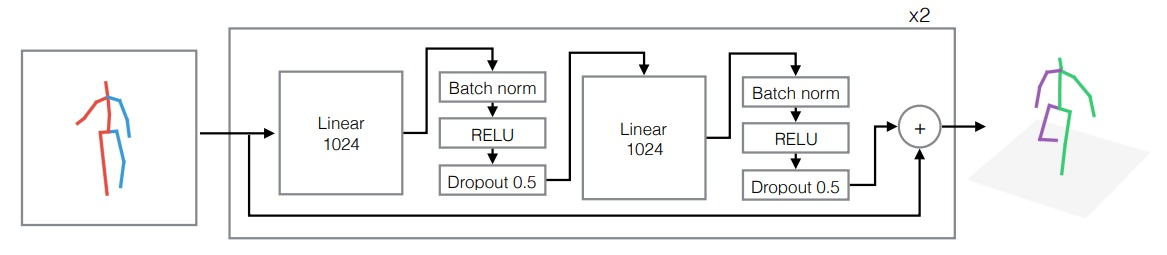
\includegraphics[width=.9\textwidth]{Chapters/3. Trans-HPE/img/martinez_model.jpeg}
    \caption[2D a 3D model]{Modelo usado por J. Martinez \cite{DBLP:journals/corr/MartinezHRL17}
    basado en una simple red neuronal multicapa usando batch normalization, dropout, Rectified
    Linear Units y residual connections.}
\label{fig:model_martinez}
\end{figure}

En la figura \ref{fig:model_martinez} se muestra el modelo usado por J. Martinez. Los datos de entrada
son las posiciones de las articulaciones del cuerpo humano, estos son incrementados de dimensión a
1024 usando la primer capa lineal, posteriormente pasa a un proceso de normalización por lotes
y son activados con una función \textit{RELU} con dropout de 50 por ciento. La salida de este modelo
es proyectada para tener una dimensión de $3n$ con $n$ como el número de articulaciones, representando
puntos en un espacio de 3 dimensiones.

Siguiendo la misma estrategia \citeauthor{DBLP:journals/corr/abs-2009-00348}
\cite{DBLP:journals/corr/abs-2009-00348} utiliza una arquitectura
basada en el Transformer presentado por \citeauthor{Vaswani} \cite{Vaswani}. Un Transformer con capas
ocultas de dimensión 512, 8 cabeza de multi-atención y bloques codificadores como se observa en la
figura \ref{fig:Liftformerfig}.

\begin{figure}[!ht]
    \centering
    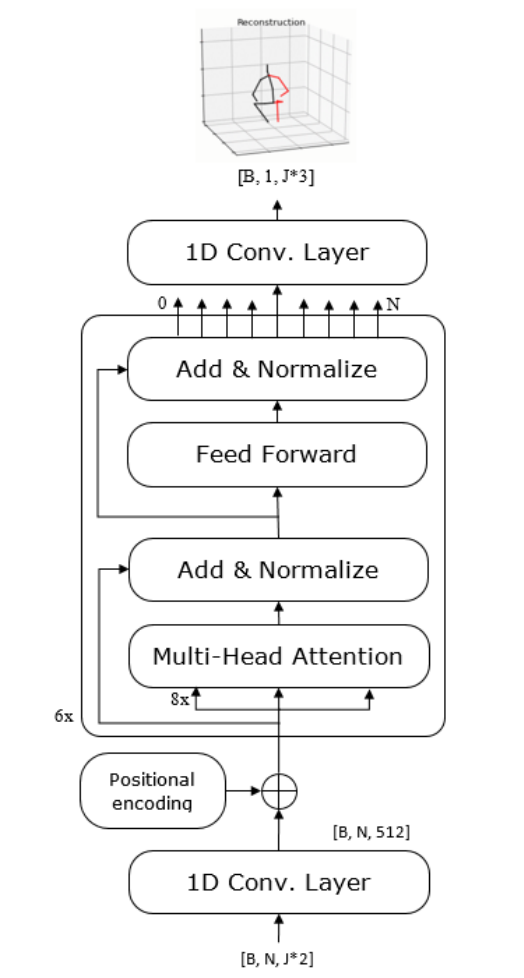
\includegraphics[width=.4\textwidth]{Chapters/3. Trans-HPE/img/poseTrans.png}
    \caption[Liftformer]{Liftformer
    \cite{DBLP:journals/corr/abs-2009-00348}, modelo basado en la parte codificadora del un Transformer.
    Predice los puntos de articulación 3D a partir de una secuencia de puntos 2D.}
\label{fig:Liftformerfig}
\end{figure}

Liftformer solo implementa la parte codificadora del modelo de
Transformer sin ningún otro cambio a este. Durante el entrenamiento utiliza como entrada una secuencia
de coordenadas representando las puntos de articulaciones en dos dimenciones. La primer mitad corresponde
a información del pasado y la segunda mitad a información del futuro generando una predicción de pose
3D correspondiente al centro de la secuencia de entrada.

Al inicio del modelo la información es reproyectada de un espacio de $[N, 34]$ a $[N, 512]$ a través
de una capa Convolucional de una dimención. En este misma etapa es inyectada la información temporal
a usando \textit{temporal embeddings}. De manera similar y dado que no es usado un decodificador
el modelo elige el token correspondiente a la mitad de los datos de entrada repoyectándolo a dimenciones
$[1, 51]$. Las 17 articulaciones y en coordenadas x, y, z estarán representadas por este vector de 51
elementos.


- Proyecto del tipo que usa transformers

Proyecto enfocado solo en Estimación de pose 2D HPE y 3D HPE considerando un solo objetivo SPPE

Para el primer caso solo martinez solo se enfoca en el segundo stage de la estimación de pose
no se usa un modelo end-to-end sino que aprovecha los modelos ya creados para estimación de pose
en 2d y

Explicar las arquitecturas usadadas
- la de martinez
- La del transformer
- La que funciona

\section{Modificación a transformers - Usando cabezas de Atención flexibles}

\section{Evaluación y comparativas}


\chapter{Detección de patologías pulmonares}
\section{Detección de Patologías en Pulmones con Rayos X}

Diferentes trabajos se han limitado a clasificar \textit{COVID-2019} y \textit{no COVID-2019} (o
neumonía), es por ello que durante este trabajo desarrollamos un sistemas más completo para {
distinguir 15 diferentes enfermedades pulmonares.

We experimentally evaluated the proposed model for diagnosis of the 15 lung diseases, obtaining
competitive results, in particular for COVID-19. We compare it with several recent works that classify
14 pathologies (excluding COVID-19); the results in terms of Area Under Curve of the Receiver Operator
Characteristic show a competitive performance of the proposed method for the ChestX-Ray14 pathologies
and a remarkable performance in detecting pneumonia from COVID-19.

In this work we developed a deep learning method that uses as BKN the ResNet50 network, a wildly
used network by the community for implementing different image analysis methods. We extend the
ChestX-Ray14 dataset by including radiographs of Normal and COVID-19 infected patients. Our training
consists of three stages, DTL from the ResNet50 pretrained in ImageNet by replacing the classification
stage by a 15 pathologies classifier, a fine-tuning stage to adjust the last convolutional layers,
and a full-tuning stage that adjusts the weights of the entire network. We demonstrate with experiments
that our proposal is able to preserve the performance of the state of the art 14 pathologies classifiers,
and at the same time achieve the state of the art performance of binaries classifiers for COVID-19.
Additionally, in order to demonstrate that the proposed model can be easily extended for other
pathologies, we implemented a binary classifier for Tuberculosis, a particular bacterial pneumonia
\cite{stirenko2018chest}, with performance comparable to \emph{ad hoc} deep learning models
\cite{puttagunta2021detection}.

in our work we also use the ChestX database \cite{wang2017chestx} and include X-rays of COVID-19 and
healthy (images of persons without known lung diseases) classes. The ChestX-ray14 contains 112,120
frontal-view (both postero-anterior and antero-posterior) chest radiographs of 30,805 unique patients.
Each image is annotated with 14 thoracic pathology labels. We enriched such a dataset with COVID-19,
pneumonia, and healthy chest radiographs. Table~\ref{table_dataset} summarizes the composition of
the dataset used in our work.

\begin{table}[!ht]
    \centering
    \begin{tabular}{| r |l | c | c | c |}
     \hline
     Class & Disease & Source & Train & Test  \\
     \hline\hline
     1  & Cardiomegaly       & 1 & 5897  & 1069 \\
     2  & Emphysema          & 1 & 3496  & 1093 \\
     3  & Effusion           & 1 & 13737 & 4658 \\
     4  & Hernia             & 1 & 4470  & 86   \\
     5  & Infiltration       & 1 & 17122 & 6112 \\
     6  & Mass               & 1 & 7862  & 1748 \\
     7  & Nodule             & 1 & 9250  & 1623 \\
     8  & Atelectasis        & 1 & 13762 & 3279 \\
     9  & Pneumothorax       & 1 & 6303  & 2665 \\
     10 & Pleural-Thick.     & 1 & 8022  & 1143 \\
     11 & Pneumonia          & 1 & 6031  & 555  \\
     12 & Fibrosis           & 1 & 9072  & 435  \\
     13 & Edema              & 1 & 6953  & 925  \\
     14 & Consolidation      & 1 & 9796  & 1815 \\
     ---&  Healthy           & 1 & 35645 & 9861 \\
     \hline
     11 & Pneumonia          & 2 & 5475  & 594  \\
     15 & COVID-19           & 2 & 2873  & 1904 \\
     ---&  Healthy           & 2 & 8661  & 1926 \\
     \hline
    \end{tabular}
    \caption{Number of chest radiography's per case in the dataset. Sources (DS): (1) ChestX-ray14,
             (2) Internet datasets compilation. Pleural-Thick. means Pleural-Thickening.}
    \label{table_dataset}
\end{table}

\subsubsection{Data Relabelling}
\label{ssec_relabelling}

In order to train our model, we use the relabelled version of the ChestX-ray14 database proposed by
the authors of CheXNet \cite{rajpurkar2018deep}.  According to \cite{rajpurkar2018deep}, the
relabelled data allows to improve the training process significantly. Such relabelling consists of
training multiple times a  neural network with the original training data set and keeping those
models with the best accuracy on the original validation set. Then, the predictions of the individual
models are averaged, and a binary detector of each pathology is computed by using a threshold that
maximizes the F1-score in all the pathologies (see Section~\ref{sec_metrics} for the F1-score
definition). Finally, each training and test datum is relabeled as positive for pathology, if it was
initially labeled as positive or the ensemble prediction is positive. However,  we define the train,
validation, and test data sets according to the original problem; \emph{i.e.}, for the original list and
only use the new labels in the training stage. Thus, we report two results: the first one on the
original test dataset and, just for reference,  with the updated labels in the Appendix.

\subsubsection{Data Preprocessing}

We keep as simple as possible the preprocessing of the radiography, we only perform a histogram
equalization and resize the data to $1024 \times 1024$ pixels.

La datos de entrada son imágenes de 1024
columnas y 1024 filas con 3 canales idénticos. Siguiente la propuesta de \textit{CheXNet}, se hace uso
de multiples funciones de perdida tipo \textit{Binary Cross-Entropy} con distintos pesos
para solventar el desbalanceamiento de clases.

\begin{equation} \label{eq:loss}
    L(\hat y, y) = \sum_{c=0}^{15} \left[ w_c^{(p)} y_c \log \hat y_c  + w_c^{(n)}  (1-y_c) \log  (1- \hat y_c)  \right],
\end{equation}

donde $y$ es el vector de etiquetas reales, $\hat y$ es el vector de etiquetas predichas,
$w_c^{(p)}$ y $w_c^{(n)}$ son los pesos para los casos positivos y negativos de cada clase $c$
respectivamente. Dichos pesos son calculados como sigue:

\begin{equation}\label{eq:weights}
    w_c^{(n)} = \frac{n_c}{N} \;\;\;\;\text{and}\;\;\;\;   w_c^{(p)} = 1-  w_c^{(n)};
\end{equation}

donde $N$ es el tamaño del conjunto de datos, y $n_c$ el número de imágenes radiográficas con
etiquetas $c$ (el número elementos del vector de la $c$-ésima clase iguales a 1). Nótese que los
pesos son inversamente proporcional al número de casos en la clase.


\section{Arquitecturas usadas}
\subsection{Vision Transformers}
\subsection{ViT con cabezas de atención Flexibles}

\section{Alternativa: CNN y Transfer Learning}

El modelo desarrollado es construido tomando \textit{CheXNet} como referencia
\cite{rajpurkar2018deep}, el cual clasifica entre 14 enfermedades
usando el conjunto de datos \textit{ChestX-Ray14} \cite{wang2017chestx}. El modelo propuesto es
construido desde cero y extiende la propuesta de \textit{CheXNet} para incluir la clasificación de
imágenes con \textit{COVID-19}.

\textit{CheXNet} es un modelo basado en redes neuronales para detectar la presencia de 14 diferentes
enfermedades de pulmón. \textit{CheXNet} Usas imagenes de Rayos X de vista frontal como entrada y
un modelo convolucional pre-entrenado como backbone \cite{rajpurkar2018deep}. El modelo backbone usado
por \textit{CheXNet} es la red \textit{DenseNet121} \cite{huang2017densely} que contiene 121 capas
convolucionales entrenadas con la base de datos de \textit{ImageNet} \cite{ILSVRC15}. Las imágenes
analizadas por el modelo pueden corresponder a vistas anterior-posterior o posterior-anterior. La
implementación de Transferencia de Conocimiento es lograda removiendo la etapa de clasificación
(formada por capas densas) mientras que la etapa convolucional previa permanece intacta funcionando
como un extractor de características. Posteriormente, una nueva etapa de clasificación construida
para la detección de 14 enfermedades es colocada en su lugar. Finalmente, la nueva red compuesta
es entrenada usando la base de datos \textit{ChestX-Ray14} manteniendo fijos los pesos
correspondientes a la etapa convolucional de la red.

Así como en \textit{CheXNet}, un modelo usado como backbone y entrenado con la base de datos de
\textit{ImageNet} define la red entrenada para detectar patologías toráxicas. Motivados por
\citeauthor{bressem2020comparing, shazia2021comparative} que muestran que una red backbone en
particular no es un elemento definitivo en el rendimiento de detección del modelo, sino el proceso
de entrenamiento. Adicionalmente \citeauthor{huang2017densely, luo2020comparison} presentan
comparaciones de modelos evaluados en la clasificación de ImageNet donde \textit{ResNet50} y
\textit{DenseNet201} obtienen un accuracy de $76\%$ y $74\%$ respectivamente. Por ello, se realiza
la elección del modelo \textit{ResNet50} como backbone en la implementación de la red convolucional.
\textit{ResNet50} fue propuesta por \citeauthor{he2016deep} y es una opción popular en la
implementación de sistemas de reconocimiento generales dado su eficiencia computacional y relativamente
sencillez de entrenamiento (por su grafo de gradientes con poco caminos) en comparación del candidato
natural \textit{DenseNet121} usando en \textit{CheXNet}, aque versiones alternativas de
\textit{CheXNet} estan disponibles \cite{chexnet_code}. A pesar de lo anterior, no se descarta el uso
e investigación en un futuro de otros modelos como backbone ya sea inclusive \textit{DenseNet} o
\textit{efficientNet} \cite{tan2019efficientnet}. Sabiendo que este mismo procedimiento puede
guiarnos a incluir nuevas patologias tales como Tuberculosis Pulmonar \cite{stirenko2018chest}; un
tipo de neumonia bacterial mayormente común en países en vías de desarrollo y también frecuentemente
reportado en pacientes con sindrome de inmunodeficiencia adquirida (AIDS) \cite{matsuura2018tuberculous}.

En la red detectora, la etapa clasificadora del modelo \textit{ResNet50} es remplazada con dos capas
densas y una operación de \textit{Dropout} intermedia con probabilidad de $25\%$. La tabla
\ref{table_resnet50} resume la arquitectura de la red.

\begin{table}[!ht]
    \centering
    \begin{tabular}{| l|c | c | r |}
    \hline
                 &     Input   &  Output    &  \\
    Layer        &   dimension & dimension  & Parameters \\
    \hline\hline
    ResNet50     &     3,1000,1000 &     2048,1,1 & 24,036,431 \\
    Flatten      &     2048        &     2048     &  --        \\
    Dense        &     2048        &     256      & 524,544    \\
    ReLU         &     256         &     256      & --         \\
    Drop-0.25  &     256         &     256      & --         \\
    Dense        &     256         &     15       &  3,855     \\
    Sigmoid      &     15          &     15       & --         \\
    \hline
    \end{tabular}
    \caption{Deep neural network architecture used in the proposed model. The Dense layers include the bias term. Drop-0.25 means a Dropout layer with a probability of 0.25.}
    \label{table_resnet50}
\end{table}

\subsubsection{Proceso de Entrenamiento}
\label{ss:archiecture}

% we present the procedure to train our models to detect the 15 pathology's (including COVID-19) from a network pre-trained with ImageNet.
\begin{enumerate}
    \item \textbf{Entrenamiento inicial}. Una vez seleccionada la red convolucional pre-entrenada
          con la base de datos de ImageNet, se reemplaza la etapa de clasificacion con por una nueva
          compuesta por dos capas densas. En la tabla \ref{table_resnet50} se presentan los detalles
          de la red \textit{ResNet50} usada en este modelo. De esta forma, la red convolucional
          \textit{ResNet50} funciona como un extractor de características; se transforma los datos
          originales (las imágenes de radiografías) en una nueva representación que contiene las
          características que permiten distinguir entre las distintas patologías. El clasificador es
          implementado agregando dos capas densas a esta red base. En la etapa de entrenamiento la
          red se comporta como como una red Perceptrón Multicapa (\textit{Multilayer Perceptron},
          MLP) donde la entrada es el tensor de características calculados por la red base o
          backbone. Para entrenar el clasificador, los pesos que corresponden a la red base son
          congelados y solamente son actualizados los pesos que pertenecen a la etapa de
          clasificación (las capas densas descritas en la tabla \ref{table_resnet50}). El
          entrenamiento se realiza durante 35 épocas conservando el mejor modelo de acuerdo al
          accuracy obtenido usando el conjunto de validación.

    \item \textbf{Fine-tuning}. Hasta este punto, el enfoque usado es un \textit{aprendizaje superficial}
          y la etapa de extracción de características está completamente desasociado de la etapa de
          clasificación. La ventaja de implementar el sistema a través de dos redes neuronales (la
          red backbone y la red MLP) es que podemos mejorar la extracción de características en
          términos de la tarea de interés. Para ello, se procede a descongelar las últimas capas
          convolucionales de la red backbone y continuar el entrenamiento en conjunto con las capas
          densas de la etapa clasificadora. Las capas a descongelar corresponden al último bloque
          construido de de la 5° etapa convolucional (\textit{layer conv5\_3}) \cite{he2016deep}.
          Así, permitimos que el tensor obtenido a la salida de la red backbone sea particularizado
          a la tarea de clasificación actual. El procedimiento de \textit{Fine-tuning} es realizado
          por 25 épocas más.

    \item \textbf{Full-tuning}. Las razones por las cuales solamente son reentrenadas las últimas
          capas convolucionales son que tenemos que lidiar con el problema del desvanecimiento del
          gradiente y el sistema completo puede terminar sobre ajustando sus parámetros a la base de
          datos de entrenamiento. El primer problema no es tan relevante en este punto, el
          rendimiento obtenido por el modelo es satisfactorio y si no fuese posible mejorar las
          mejorar los parámetros de las capas convolucionales tampoco sufren un deterioro. El segundo
          problema es de importancia si la muestra de imágenes radiográficas son suficientemente
          representativas de las patologías de interés. Puesto que el sistema es suficientemente
          general para predecir el conjunto de imágenes de prueba correctamente. En este trabajo
          consideramos que tenemos suficientes datos y por lo tanto, como etapa final del entrenamiento
          se realiza una afinación completa del modelo. Esto es, entrenando completamente la red,
          la etapa de extracción de características (backbone) y la etapa de clasificación (MLP).
          Para evitar el over-fitting, el entrenamiento es continuado solamente por 10 épocas
          conservando el mejor modelo de acuerdo al accuracy obtenido en el conjunto de validación.

\end{enumerate}

Similar a \citeauthor{rajpurkar2018deep}, usamos, al inicio de cada etapa de entrenamiento, las
imágenes de entrenamiento son volteadas horizontalmente con 0.5 de probabilidad como técnica de
augmentation de datos.

La salida de la red es un vector de tamaño igual a el número de patologias detectadas, 15. Cada
elemento del vector $\tilde y_i \in [0,1]$ puede ser interpretado como la probabilidad que la
i-ésima patología esta presente en la imagen analizada. El vector $\tilde y$ no necesariamente tiene
que sumar 1, puesto que varias patologias pueden estar presentes en la radiografía. Una patologias
detectada como positiva ocurre si  $\tilde y > \theta$, donde $\theta$ es el umbral. El valor típico
para este umbral es de $0.5$ y puede ser modificado dependiendo del análisis de la curva del \textit{Receiver
Operator Characteristic}, o \textit{Curva ROC}. Como algoritmo de entrenamiento se usa \emph{Adam}
\cite{kingma15adam} con un factor de aprendizaje (LR) de $1\times 10^{-4}$, parámetros de inercia
$\beta_1=0.9$ y $\beta_2=0.999$ con un descaimiento (LR-decay) de $0.1$ si después de 10 iteraciones
no se detecta una reducción en el valor de la función de pérdida mayor a $1\times 10^{-4}$ (plateau
escape).

\subsubsection{Transfer Learning para la detección de Neumonía por Tuberculosis}

El propósito de esta sección es demostrar que el backbone (el modelo ResNet50) del modelo propuesto
y entrenado con las 15 patologías mencionadas anteriormente, puede ser la base para desarrollar
detectores para otras enfermedades de pulmón. La idea en esta etapa es no repetir el proceso
completo de entrenamiento sino usar en vez una simple estrategia de Transfer Learning. Así, se
procede a extender el modelo para detectar (junto con las otras enfermedades) neumonía causada por
Tuberculosis \cite{stirenko2018chest}, un tipo de neumonía bacterial común en paises en estado vias
de desarrollo y también frecuentemente reportado en pacientes con sindrome de inmunodeficiencia
adquirida (AIDS) \cite{matsuura2018tuberculous}. El dataset considerado incluye casos de
\textit{Tuberculosis} y \textit{no Tuberculosis} pero es
importante aclarar que la condición en particular de los casos de \textit{no Tuberculosis} no es
especificada por completo, es decir, incluyen tanto pacientes saludables como pacientes con otras
afecciones.

\begin{table}[!ht]
    \centering
    \begin{tabular}{| r |l | c | c | c |}
     \hline
     Class & Disease & Source & Train & Test  \\
     \hline\hline
     16  & Tuberculosis        & 3 & 888   & 488  \\
     ---&  Non-Tuberculosis     & 3 & 6000  & 1600 \\
     \hline
    \end{tabular}
    \caption{Number of chest radiography's from patients with and without Tuberculosis.}
\label{table_dataset_tb}
\end{table}

La base de datos (indicada proveniente de la fuente 3 en la tabla \ref{table_dataset_tb}) está
compuesta por radiografías provenientes de: TBX11K dataset \cite{liu2020rethinking},
India (DA and DB) dataset \cite{chauhan2014role}, Montgomery County dataset \cite{jaeger2014two}, y
Shenzhen Hospital dataset \cite{jaeger2014two}. En este trabajo se usa las listas originales para el
entrenamiento y Evaluación definidos para este dataset.

Para poder detectar Tuberculosis, se realiza la implementación de un clasificador binario usando como
backbone la red ResNet50 entrenada previamente para la detección de las 15 patologías anteriores.
La nueva rama de clasificación incluye dos nuevas capas densas (con sus respectivas funciones de
activación). Conservamos los parámetros correspondientes al backbone no entrenables y solo se entrena
las nuevas capas densas usando la estrategia mencionada en la subsección de {\bf Initial Training}
\ref{ss:archiecture} con el optimizador, factor de aprendizaje y otros parámetros sin cambios y
\textit{Weighted Binary Cross-Entropy} como función de pérdida similar a \eqref{eq:loss}. Este modelo
extendido aún detecta las 15 enfermedades comentadas previamente con una salida binaria extra para
Tuberculosis. La arquitectura extendida incluyendo la nueva rama está descrita en la tabla
\ref{table_resnet50_tb}.

\begin{table}[!ht]
    \centering
    \begin{tabular}{| l| c | c | r |}
     \hline
                 &  Input       & Output           &   \\
    Layer        &  dimension    & dimension        & Parameters \\
    \hline\hline
    Initial Backbone & & & \\ \hline
    ResNet50     &  3,1000,1000 &     2048,1,1     & 24,036,431 \\
    Flatten      &     2048     &     2048         &  --        \\
    Dense        &     2048     &     256          & 524,544    \\
    ReLU         &     256      &     256          & --         \\
    Drop-0.25    &     256      &     256          & --         \\
    \hline
    Additional Branch & & & \\ \hline
    Dense$^\ast$ &     256      &     128          &  38,896     \\
    ReLU         &     128      &     128          & --         \\
    Drop-0.20    &     128      &     128          & --         \\
    Dense$^\ast$ &     128      &      1           &  129       \\
    Sigmoid      &      1       &      1           & --         \\
     \hline
    \end{tabular}
    \caption{Deep neural network architecture used in the extended model with the Tuberculosis branch. Dense layers include the bias term and $^\ast$ indicates trainable layers.}
\label{table_resnet50_tb}
\end{table}

\begin{figure}[htp]
    \centering
    {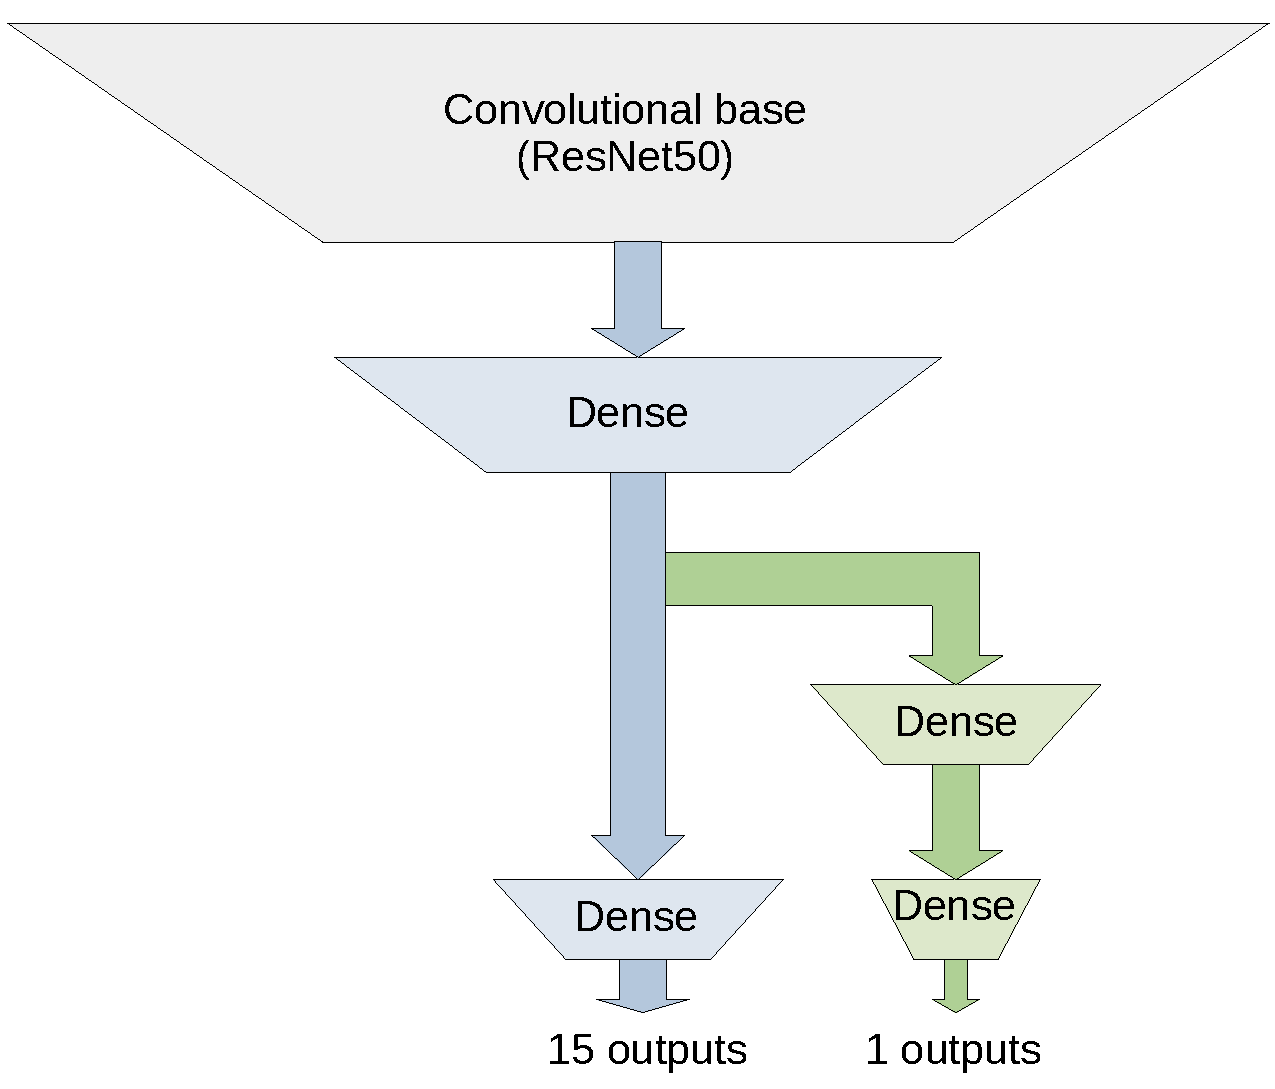
\includegraphics[width=0.5\textwidth]{Chapters/4. ViT-Lung/images/tb_net.pdf}}
\caption{Scheme of the extension of the 15 pathology detector including a new branch for Tuberculosis detection.}
\label{net_tb}
\end{figure}


\subsubsection{Métricas de Evaluación}

Considerando un problema de clasificación binario donde cada radiografia tiene una etiqueta
$y = \{1, 0\}$ con $1$ indicando la presencia del padecimiento en el paciente y $0$ significando
que se encuentra sano, el detector puede tener dos posibles resultados: una detección positiva (P)
para la enfermedad o una detección negativa (N). La tabla \ref{table_cm} muestra la caracterización
de la etiqueta predicha de acuerdo a los valores reales (Ground Truth, GT). Si un paciente enfermo
es correctamente detectado, tenemos un \textit{Verdadero Positivo} (True Positive, TP) y si la
predicción falla, es una \textit{Falso Positivo} (False Negativo, FN). Por otro lado, si una etiqueta
positiva es erroneamente predicha en un paciente saludable entonces tenemos un \textit{Falso Positivo}
(False Positive, FP), y si el paciente saludable es correctamente predicho es un
\textit{Verdadero Negativo} (True Negative, TN). La tabla \ref{table_cm} muestra la \textit{Matiz de
Confusión} con el conteo de cada tipo de predicción en el conjunto de prueba.

\begin{table*}[!ht]
    \centering
    \begin{tabular}{ccccl}
    %\cline{3-4}
    &  & \multicolumn{2}{ c }{Prediction} \\
    %\cline{3-4}
    \multicolumn{1}{c}{}& & Positive & Negative &    \\
    \cline{3-4}
    \multicolumn{1}{c}{\multirow{6}{*}{GT} } &
    \\
    \multicolumn{1}{c}{} & Disease & TP & FN   &  $ \longrightarrow  R = \frac{TP}{TP+FN}$  \\
    \\
    \cline{3-4}
    \multicolumn{1}{ c }{}                    &
    \\
    \multicolumn{1}{c}{} & No-Disease & FP & TN   &  $ \longrightarrow S = \frac{TN}{FP+TN}$   \\
    \\
    \cline{3-4}
    \\
    & & $\downarrow$ & $\downarrow$ & \\
    \multicolumn{1}{c}{} &       & $P = \frac{TP}{FP+FP}$  & $NPV = \frac{TN}{FN+TN}$ &
    \end{tabular}
    \caption{
    Interpretation of the test results (prediction) according to the ground truth (GT). Metrics are calculated as the ratio between the diagonal element and the sum per row or column, as the case may be.  R, recall or sensitivity; S, specificity; P, precision; NPV, negative prediction value}
    \label{table_cm}
\end{table*}

Para este trabajo asumimos que una patología en particular es correctamente detectada si su
correspondiente puntaje en el vector de predicho es más significante que cierto umbral. En particular,
asumimos un umbral igual para todas las patologías de $0.5$. Usando la Matriz de Confusión podemos
definir varias métricas de rendimiento.

\begin{enumerate}
    \item Accuracy ($A$). Esta métrica es quizás la más obvia. Corresponde al razón de los datos
          predichos correctamente sobre el total.
    \begin{equation}
        \label{eq:accuracy}
        A = \frac{TP+TN}{TP+TN+FP+FN}.
    \end{equation}

    \item Recall o Sensibility ($R$). Es la fracción de pacientes con enfermedades conrrectamente
          detectados. Esta metrica también es conocida como Tasa de Verdaderos Positivos (True
          Positive Rate, TPR), la tasa de detecciones correctas.

    \item Specificity ($S$). It is the fraction of patients without the disease that are correctly detected.

    \item False Positive Rate ($FPR$). The rate of false detections of the disease can be calculated with
    \begin{equation}
        \label{eq:FPR}
        FPR = 1- S,
    \end{equation}
    where $S$ is the Specificity.

    \item Precision ($P$). This is the fraction of the predicted as positives that really have the disease, also known as the True Positive Rate ($TPR$).

    \item $F_1$--score ($F_1$). The Recall metric can be bypassed if all the data tested are predicted positive regardless of the evidence. In such a case, $ FN = 0 $  and it result in $ R = 1 $; see the formula for Precision in Table \ref{table_cm}. Similarly, the Precision metric is mocked if all the tested data are predicted as negative. In this other case we will have $FPs = 0$, which implies $P = 1$. Since it is unfeasible to simultaneously cheat both metrics, then an imbalance between them indicates a bias in any of the ways described above. Therefore, it is more informative as a performance measure to use the geometric mean of both metrics.
    \begin{equation}
        \label{eq:f1}
        F_1 = \frac{2\; P \, R}{P + R}.
    \end{equation}

    \item Area Under Curve of Receiver Operator Characteristic (AUC-ROC). The receiver operator characteristic curve is a graph showing the diagnostic capabilities of binary classifiers. We have said that a particular pathology is positively detected if its predicted score is more significant than a given threshold. Then, adjusting such a threshold down allows, in general, to increase the TPR, although the FPR may also be increased. The ROC results of plotting values of TPR vs. FPR  by varying the threshold in the interval $[0,1]$. The AUC corresponds to the area under this ROC curve.

\end{enumerate}


\chapter{Conclusiones y Trabajo Futuro}
\begin{figure}[b]
    \centering
    \begin{subfigure}{0.4\textwidth}
        \centering
        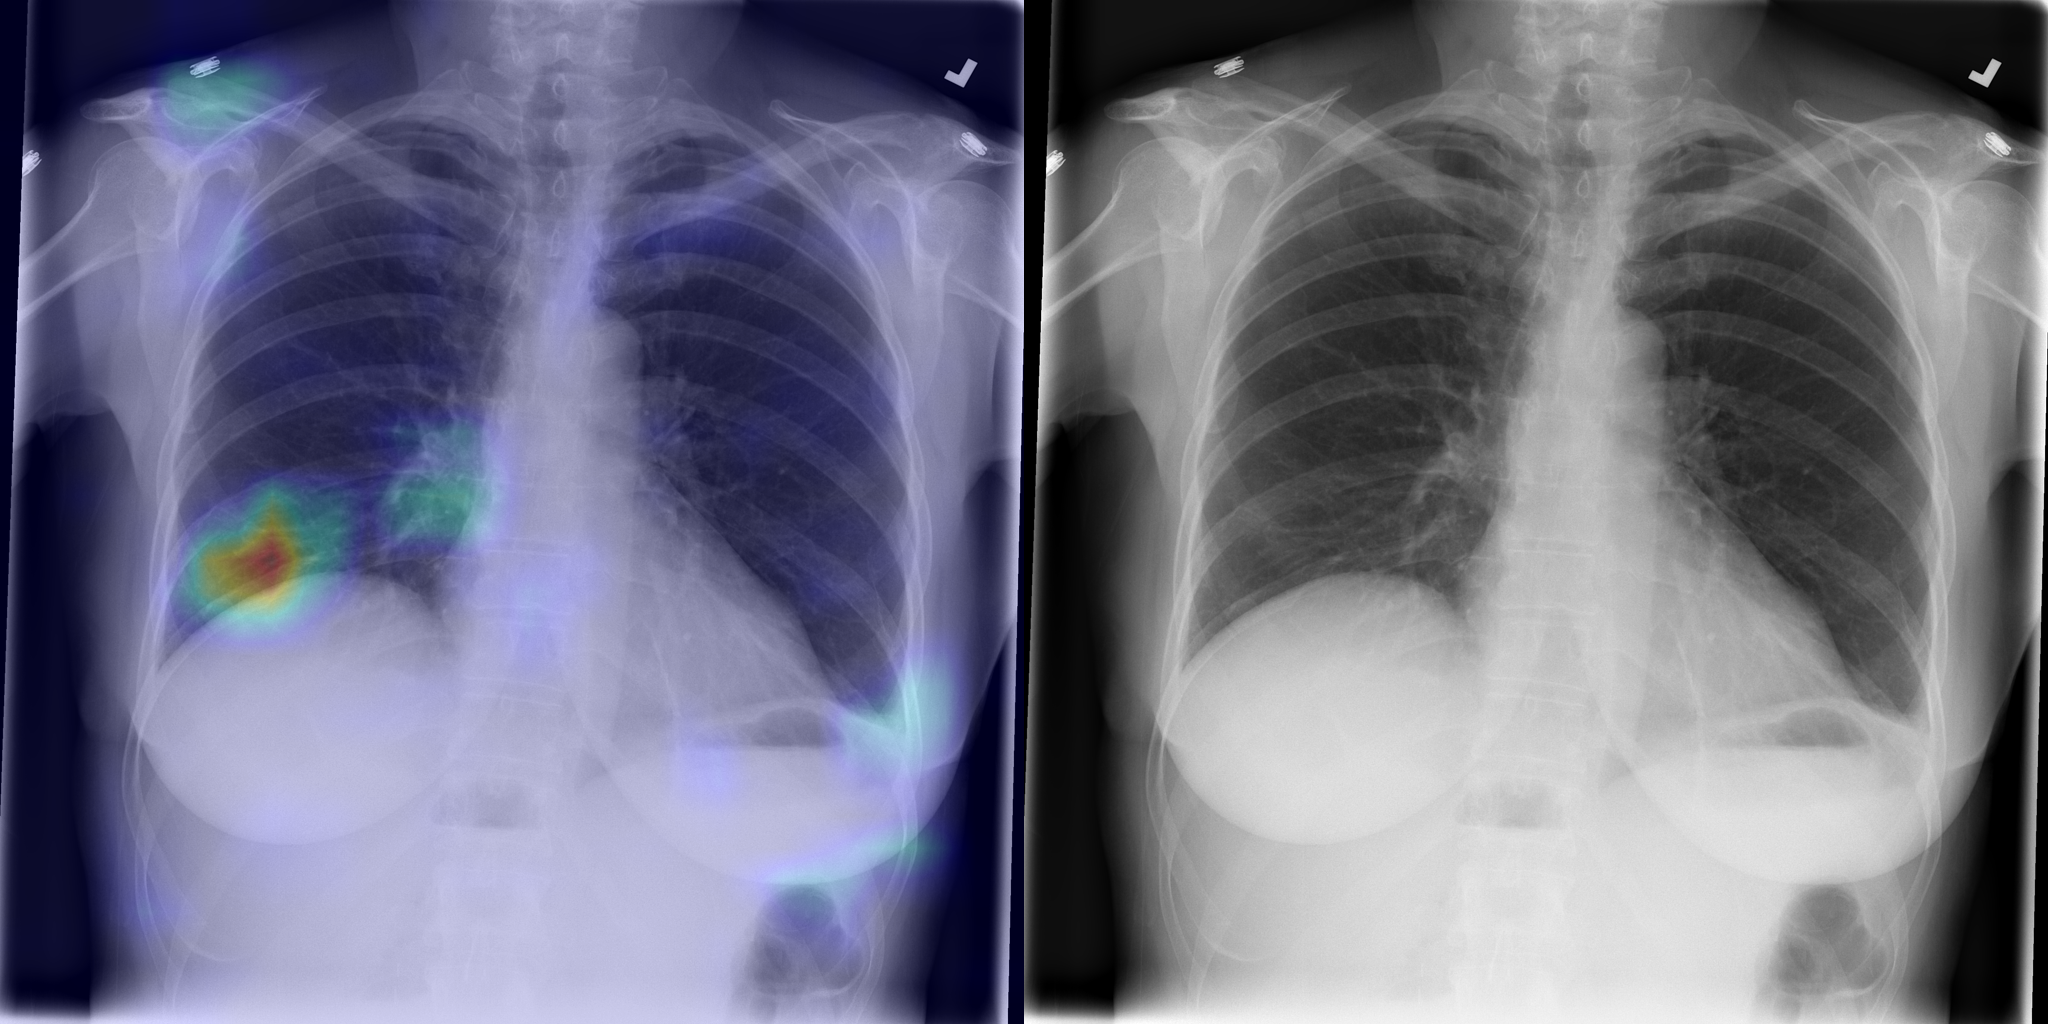
\includegraphics[width=1.0\textwidth]{Chapters/5. Conclusiones/img/Atelectasis/1_1_00000147_001.png}
    \end{subfigure}
    \begin{subfigure}{0.4\textwidth}
        \centering
        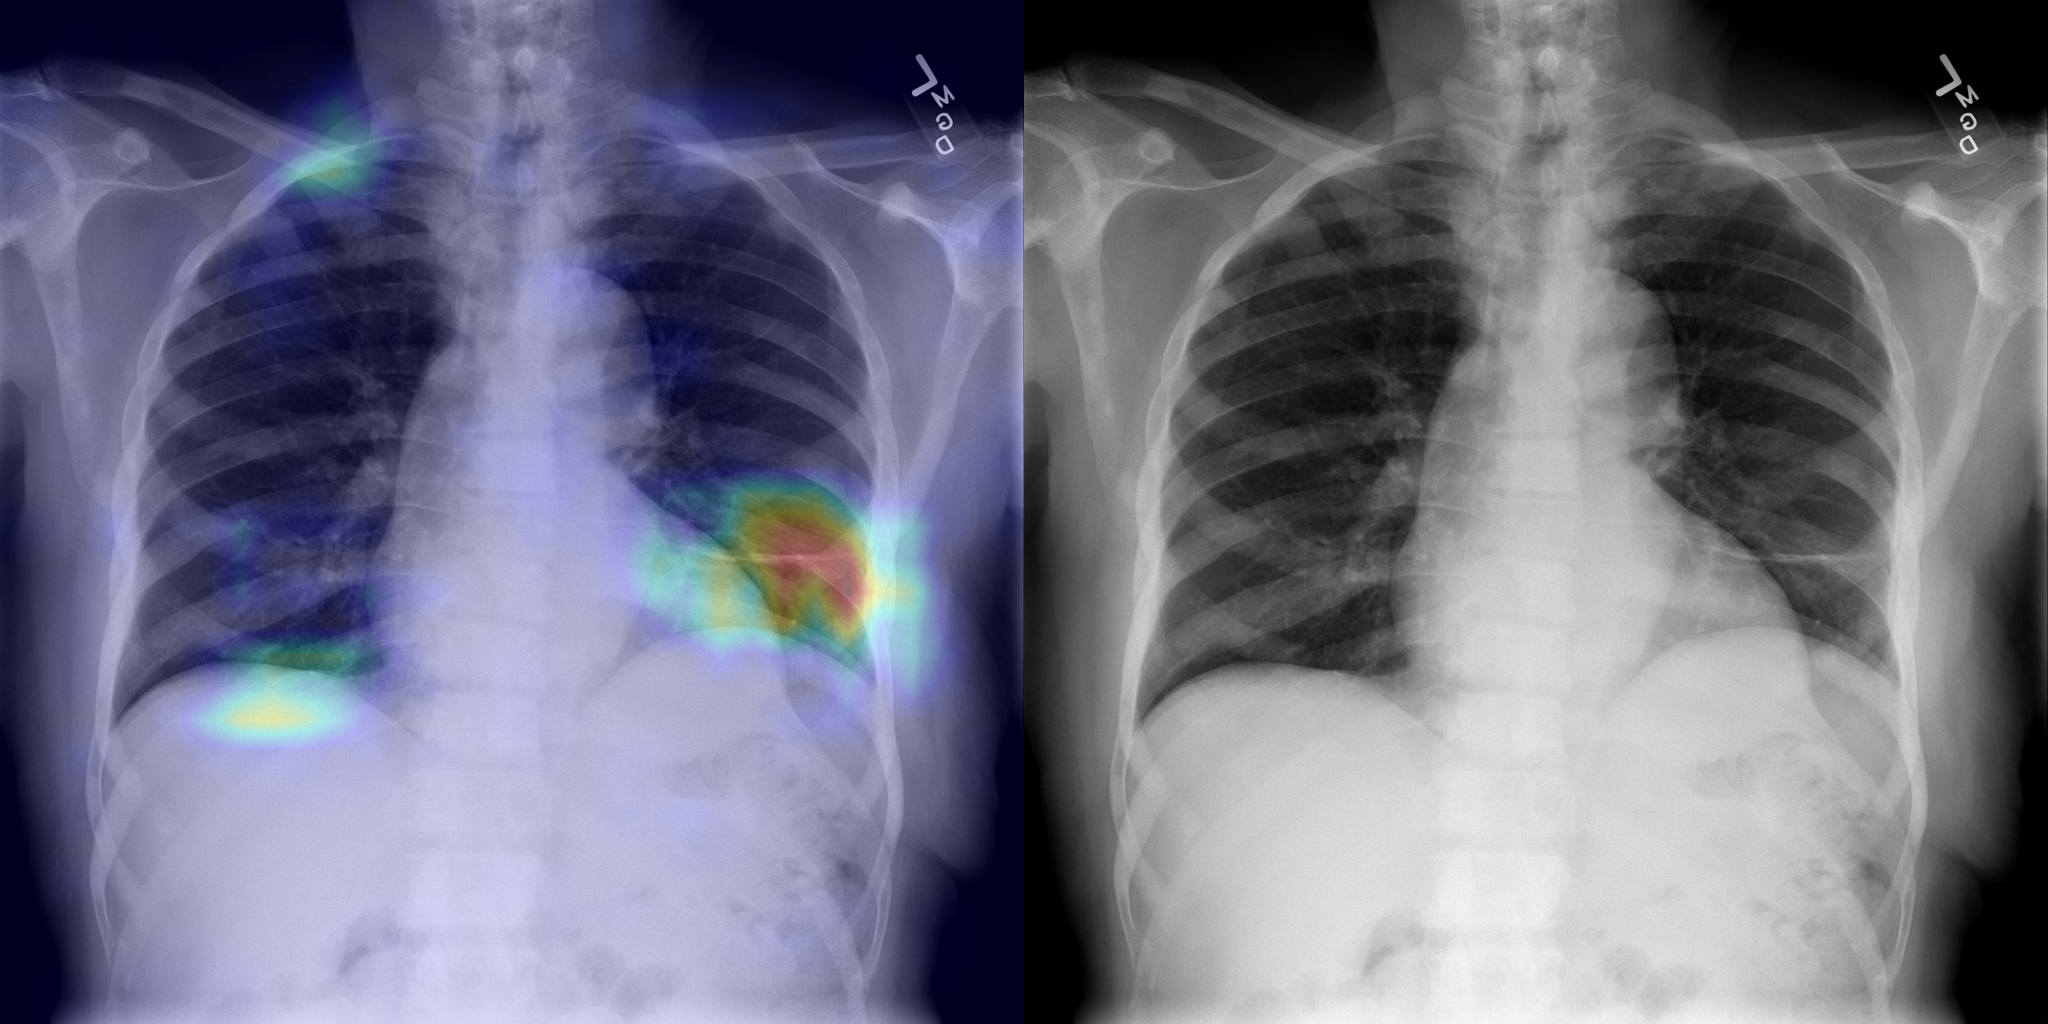
\includegraphics[width=1.0\textwidth]{Chapters/5. Conclusiones/img/Atelectasis/1_1_00000149_002.png}
    \end{subfigure}
    \begin{subfigure}{0.4\textwidth}
        \centering
        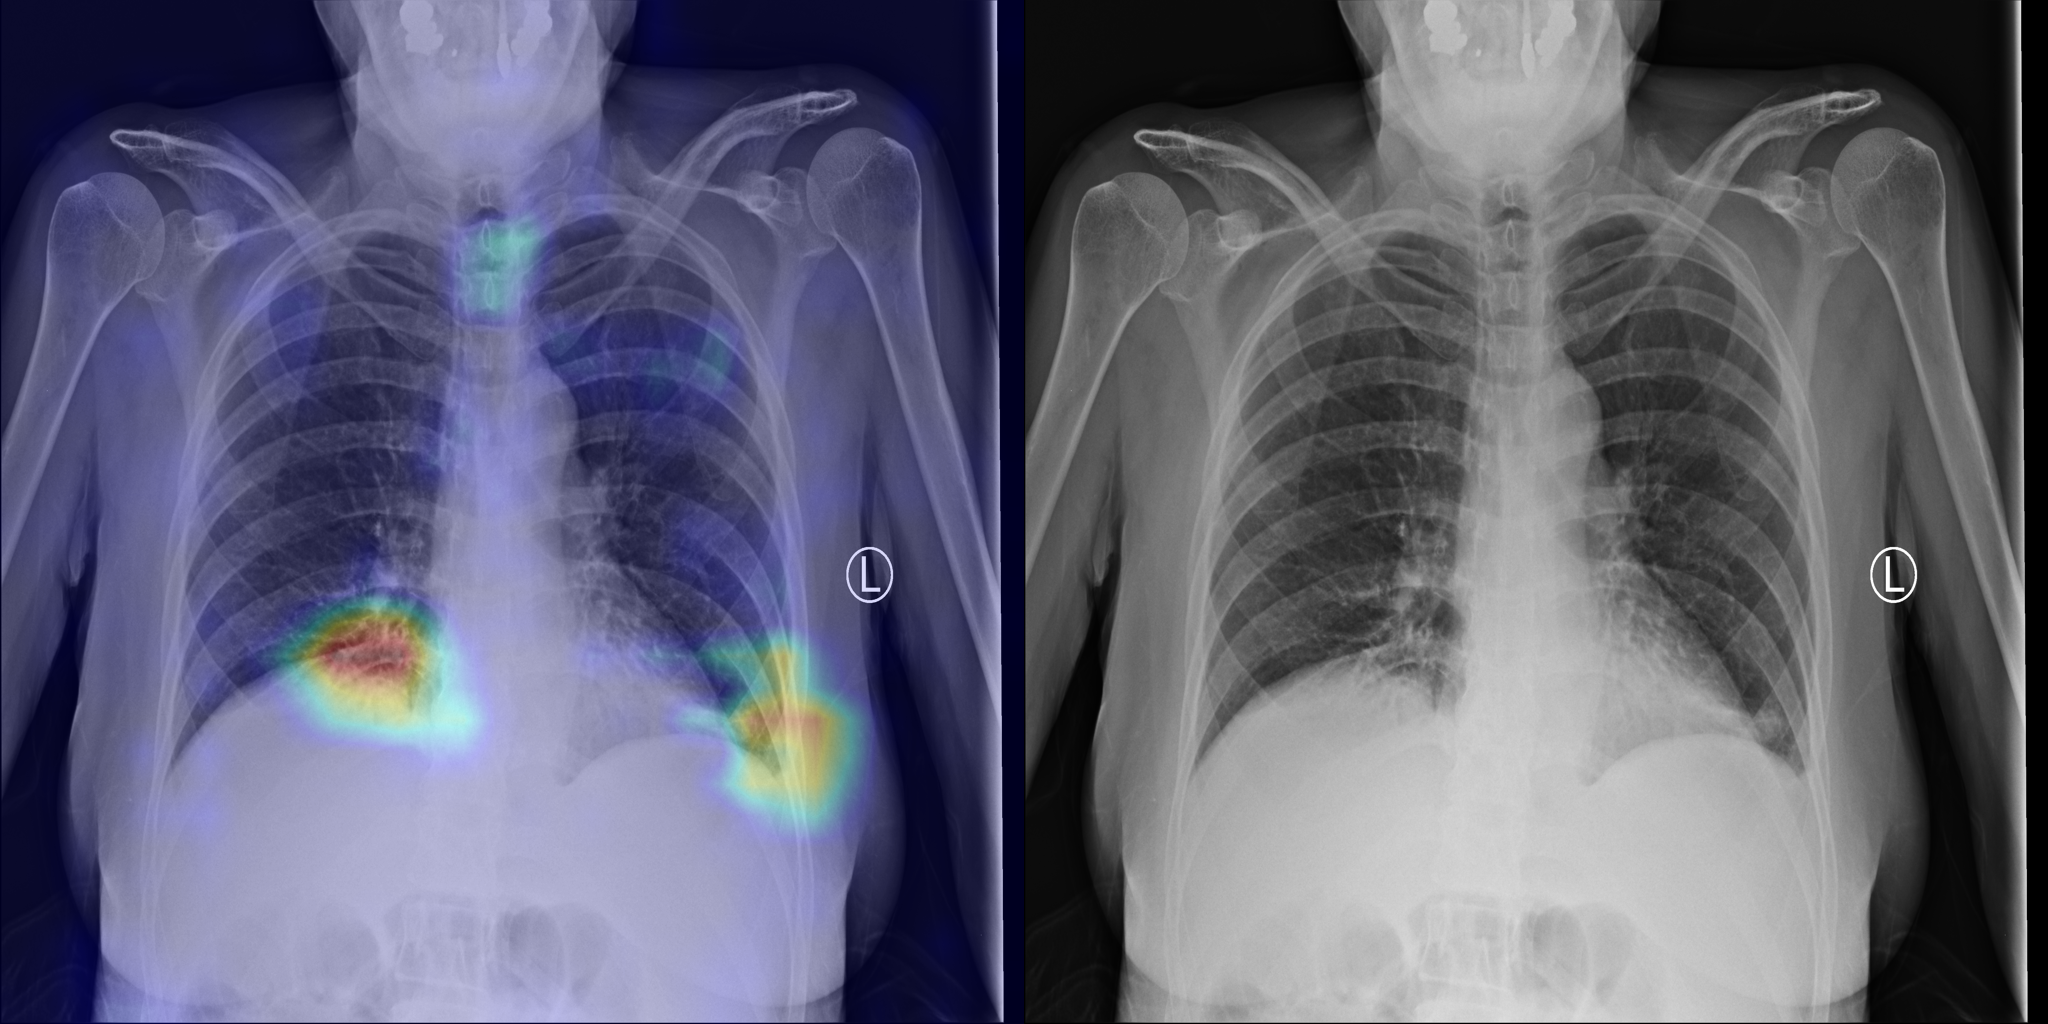
\includegraphics[width=1.0\textwidth]{Chapters/5. Conclusiones/img/Atelectasis/1_1_00000150_003.png}
    \end{subfigure}
    \begin{subfigure}{0.4\textwidth}
        \centering
        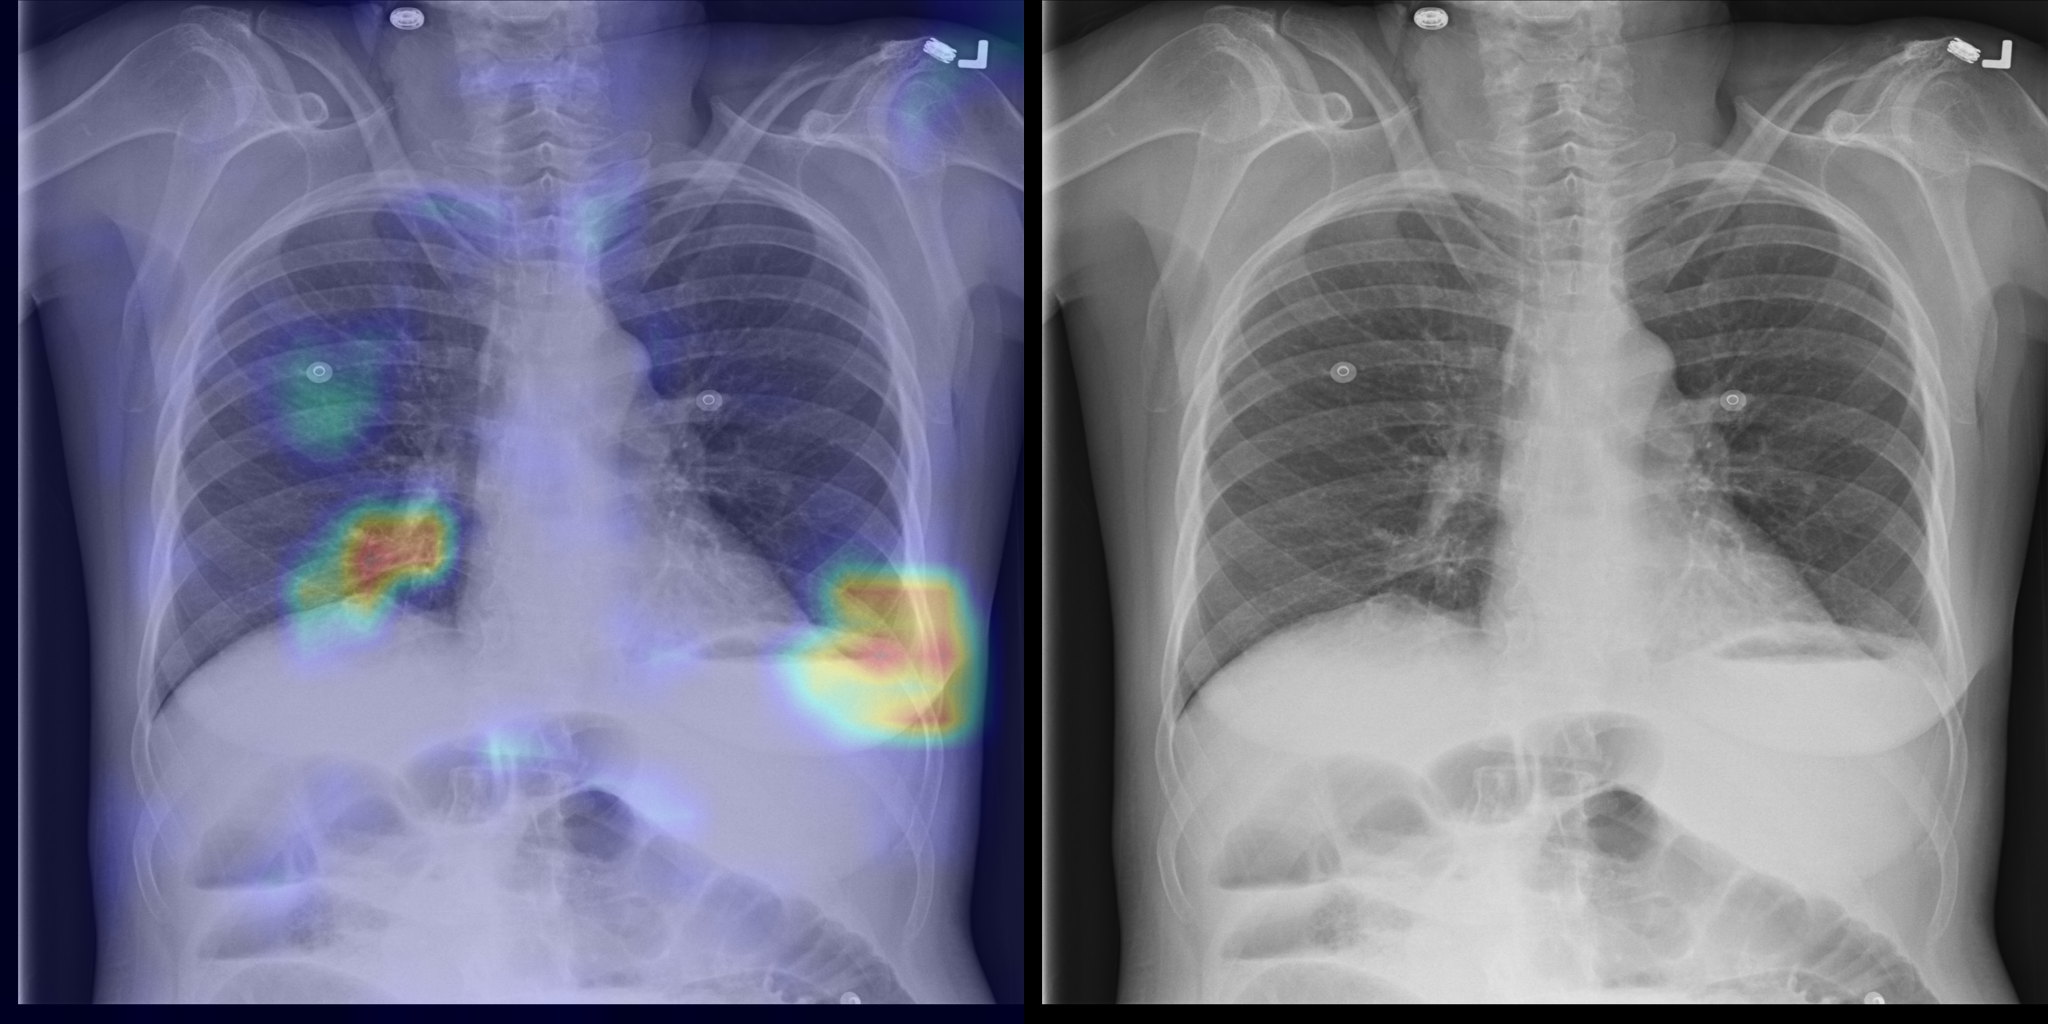
\includegraphics[width=1.0\textwidth]{Chapters/5. Conclusiones/img/Atelectasis/1_1_00000150_004.png}
    \end{subfigure}
    \begin{subfigure}{0.4\textwidth}
        \centering
        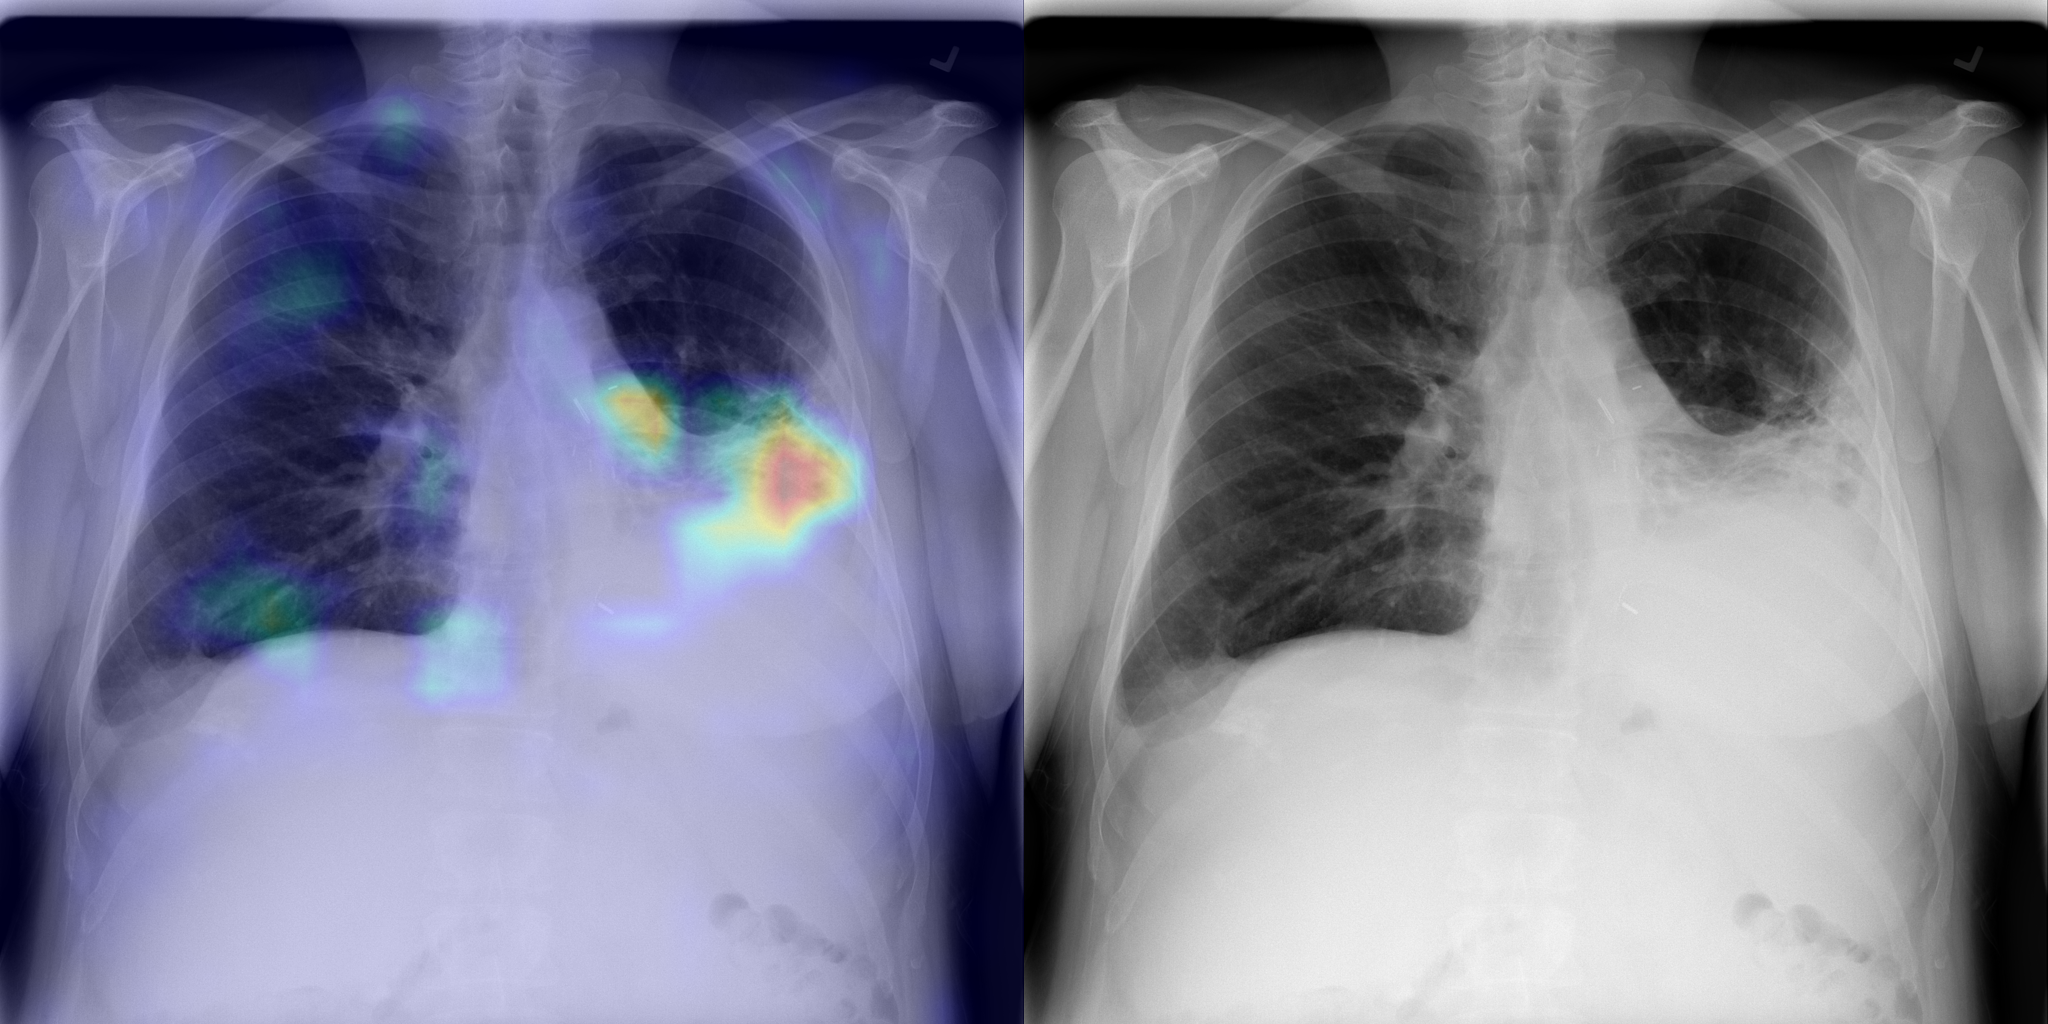
\includegraphics[width=1.0\textwidth]{Chapters/5. Conclusiones/img/Atelectasis/1_1_00000467_000.png}
    \end{subfigure}
    \begin{subfigure}{0.4\textwidth}
        \centering
        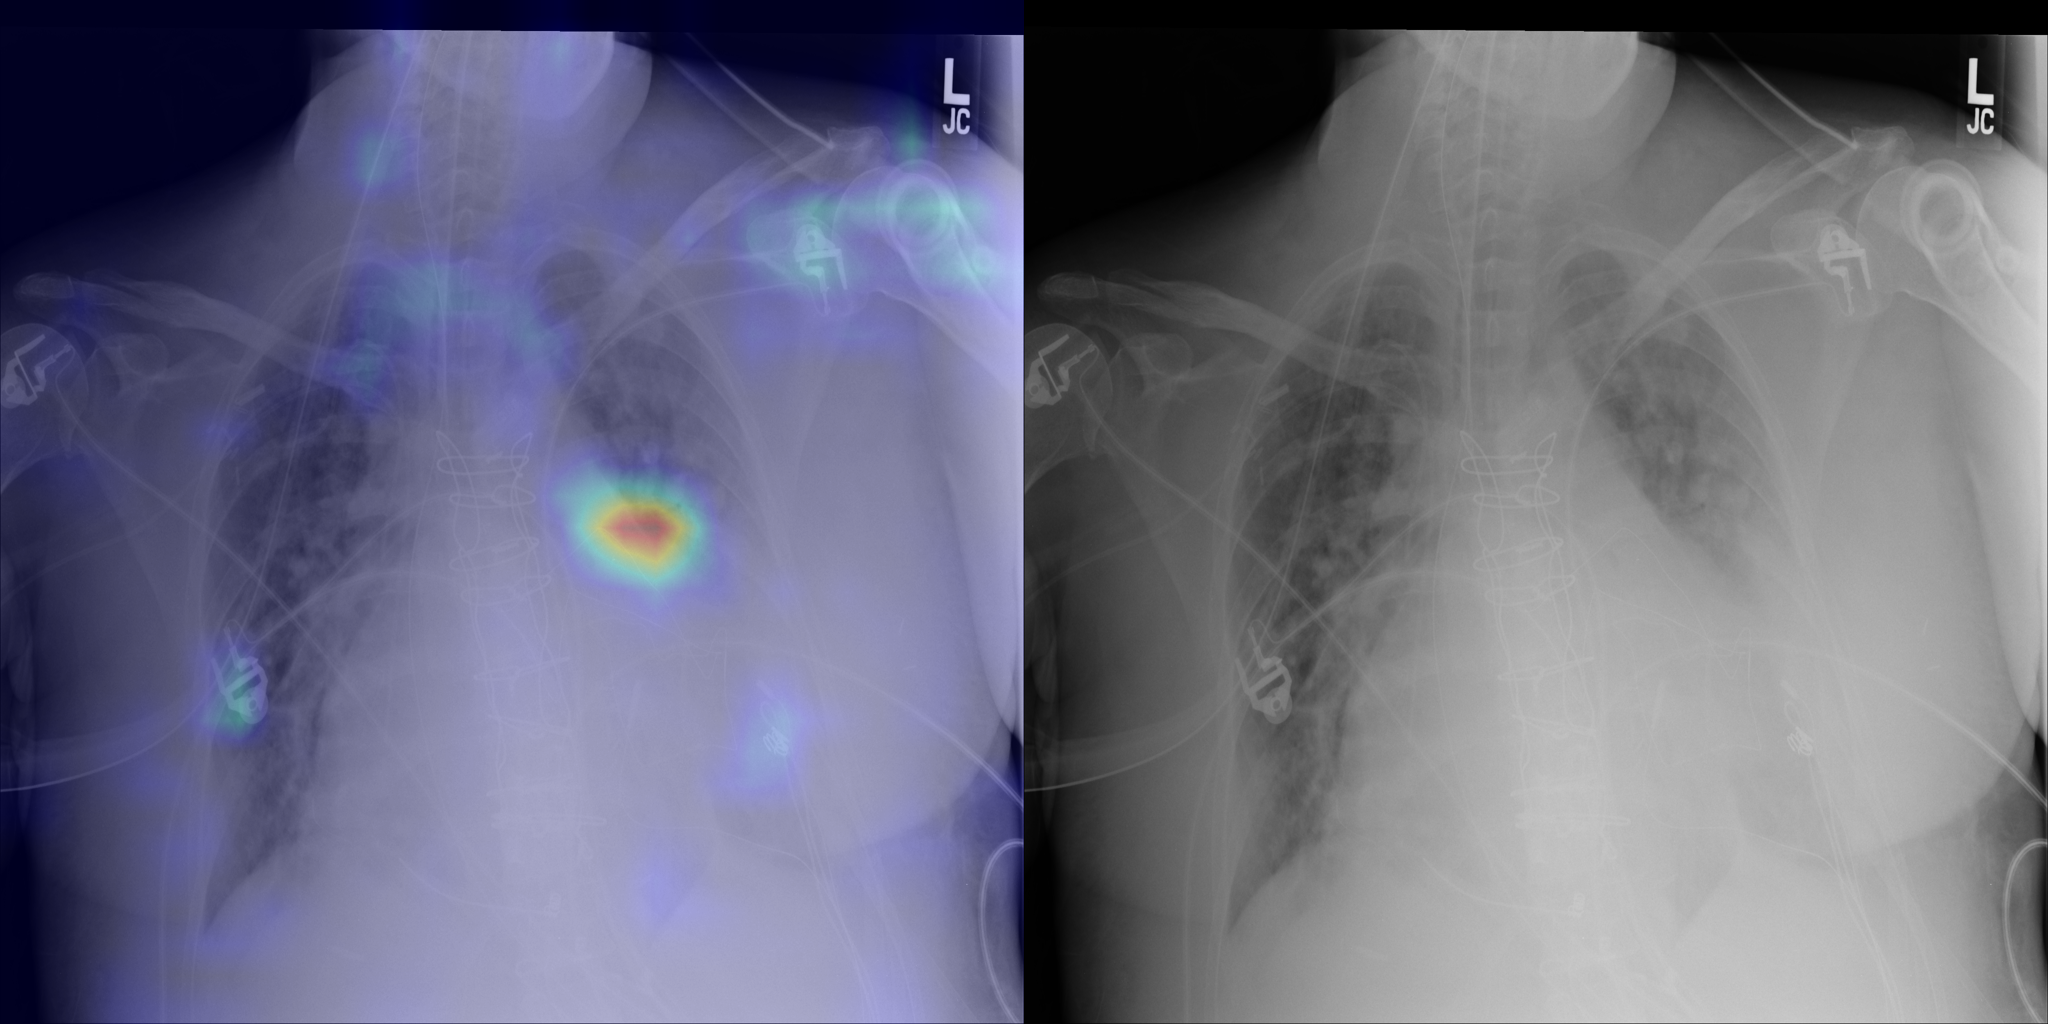
\includegraphics[width=1.0\textwidth]{Chapters/5. Conclusiones/img/Atelectasis/1_1_00000032_036.png}
    \end{subfigure}
    \begin{subfigure}{0.4\textwidth}
        \centering
        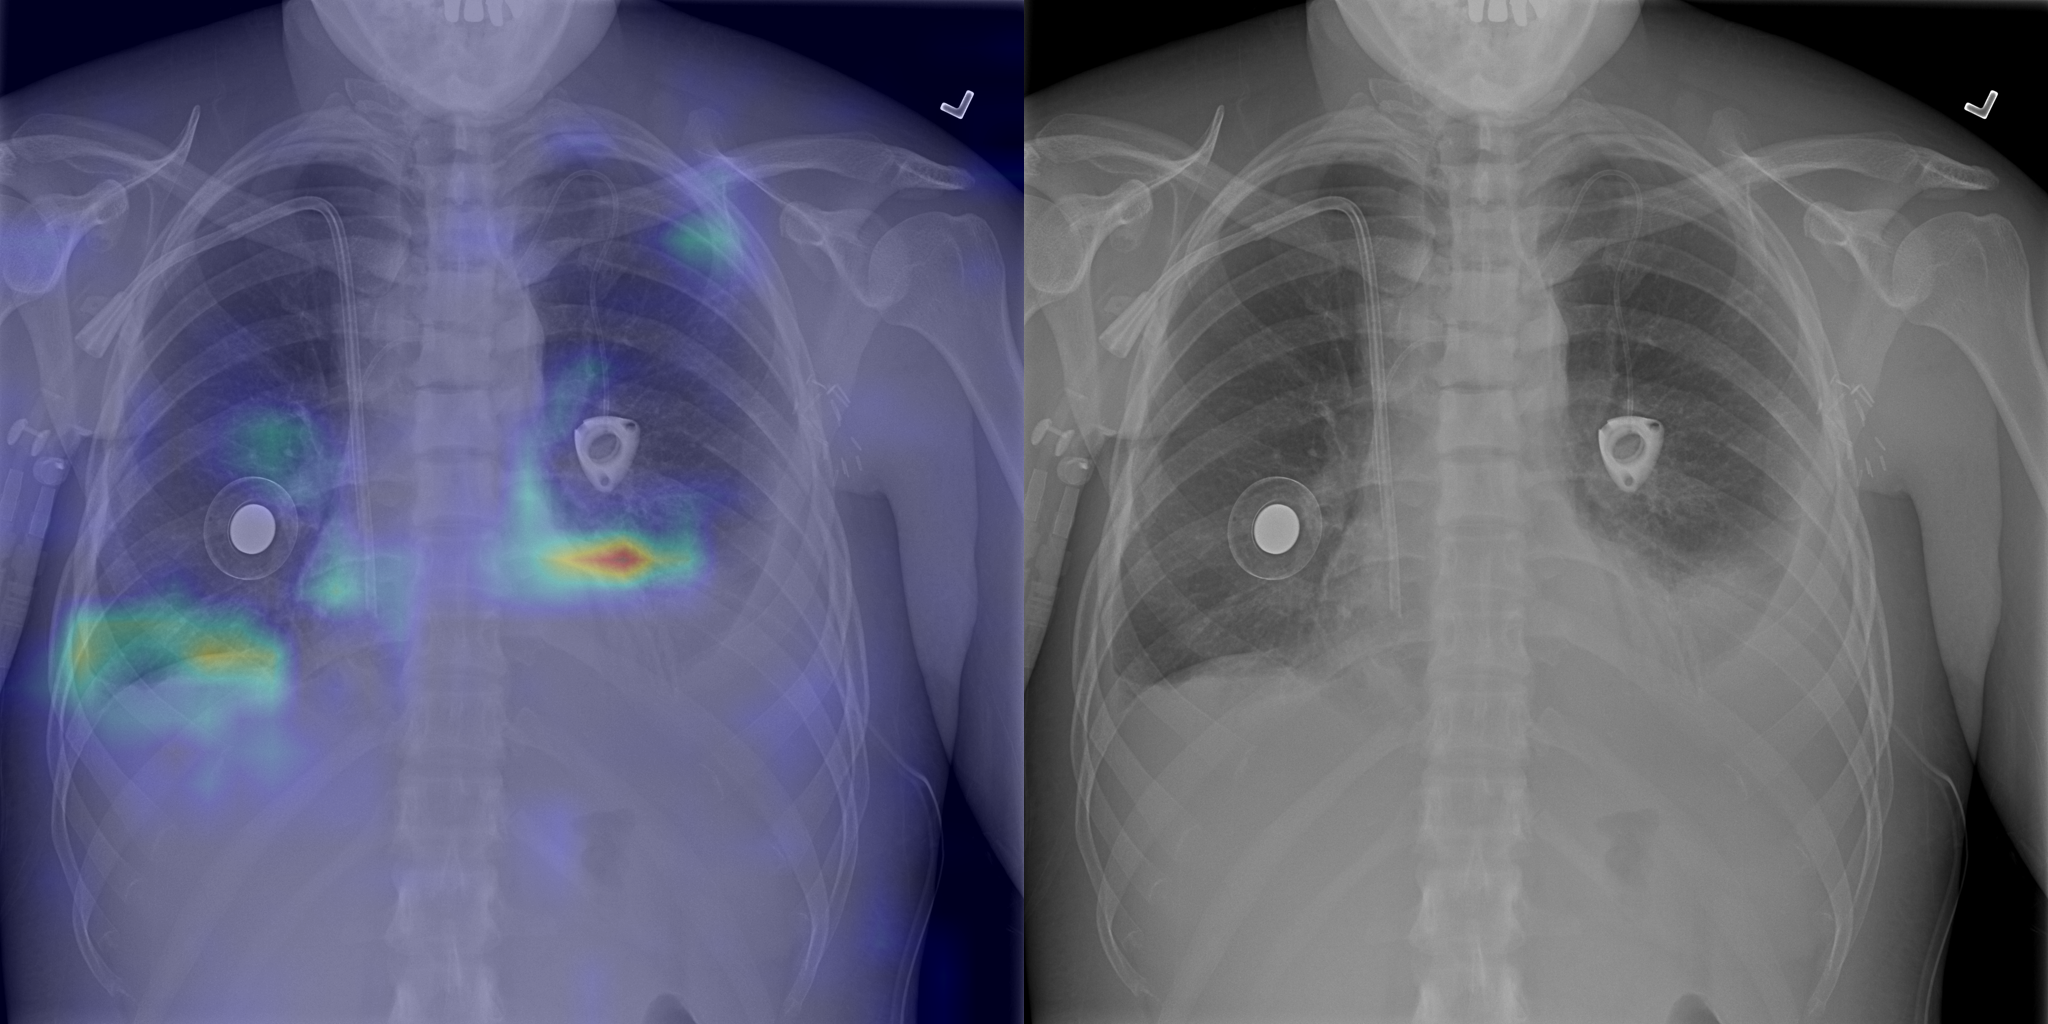
\includegraphics[width=1.0\textwidth]{Chapters/5. Conclusiones/img/Atelectasis/1_1_00029596_022.png}
    \end{subfigure}
    \begin{subfigure}{0.4\textwidth}
        \centering
        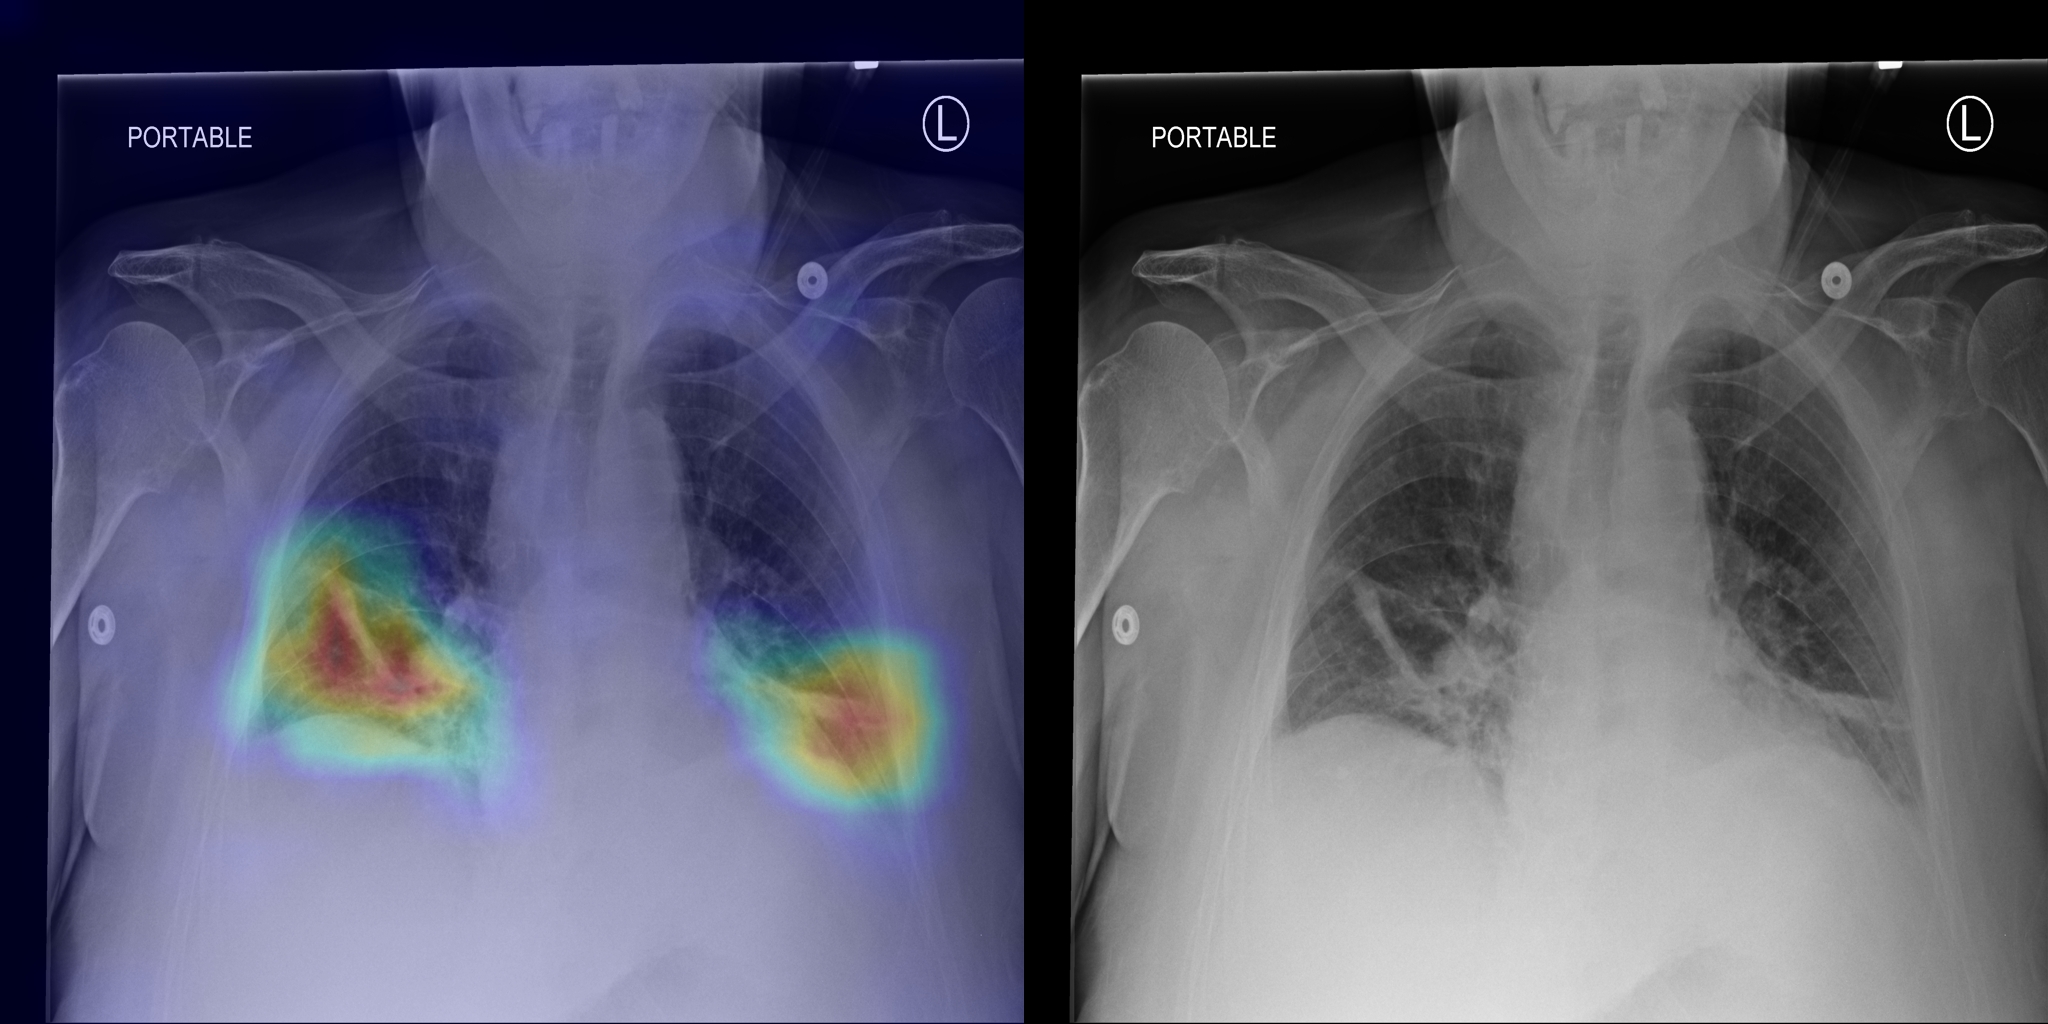
\includegraphics[width=1.0\textwidth]{Chapters/5. Conclusiones/img/Atelectasis/1_1_00030408_000.png}
    \end{subfigure}
    \begin{subfigure}{0.4\textwidth}
        \centering
        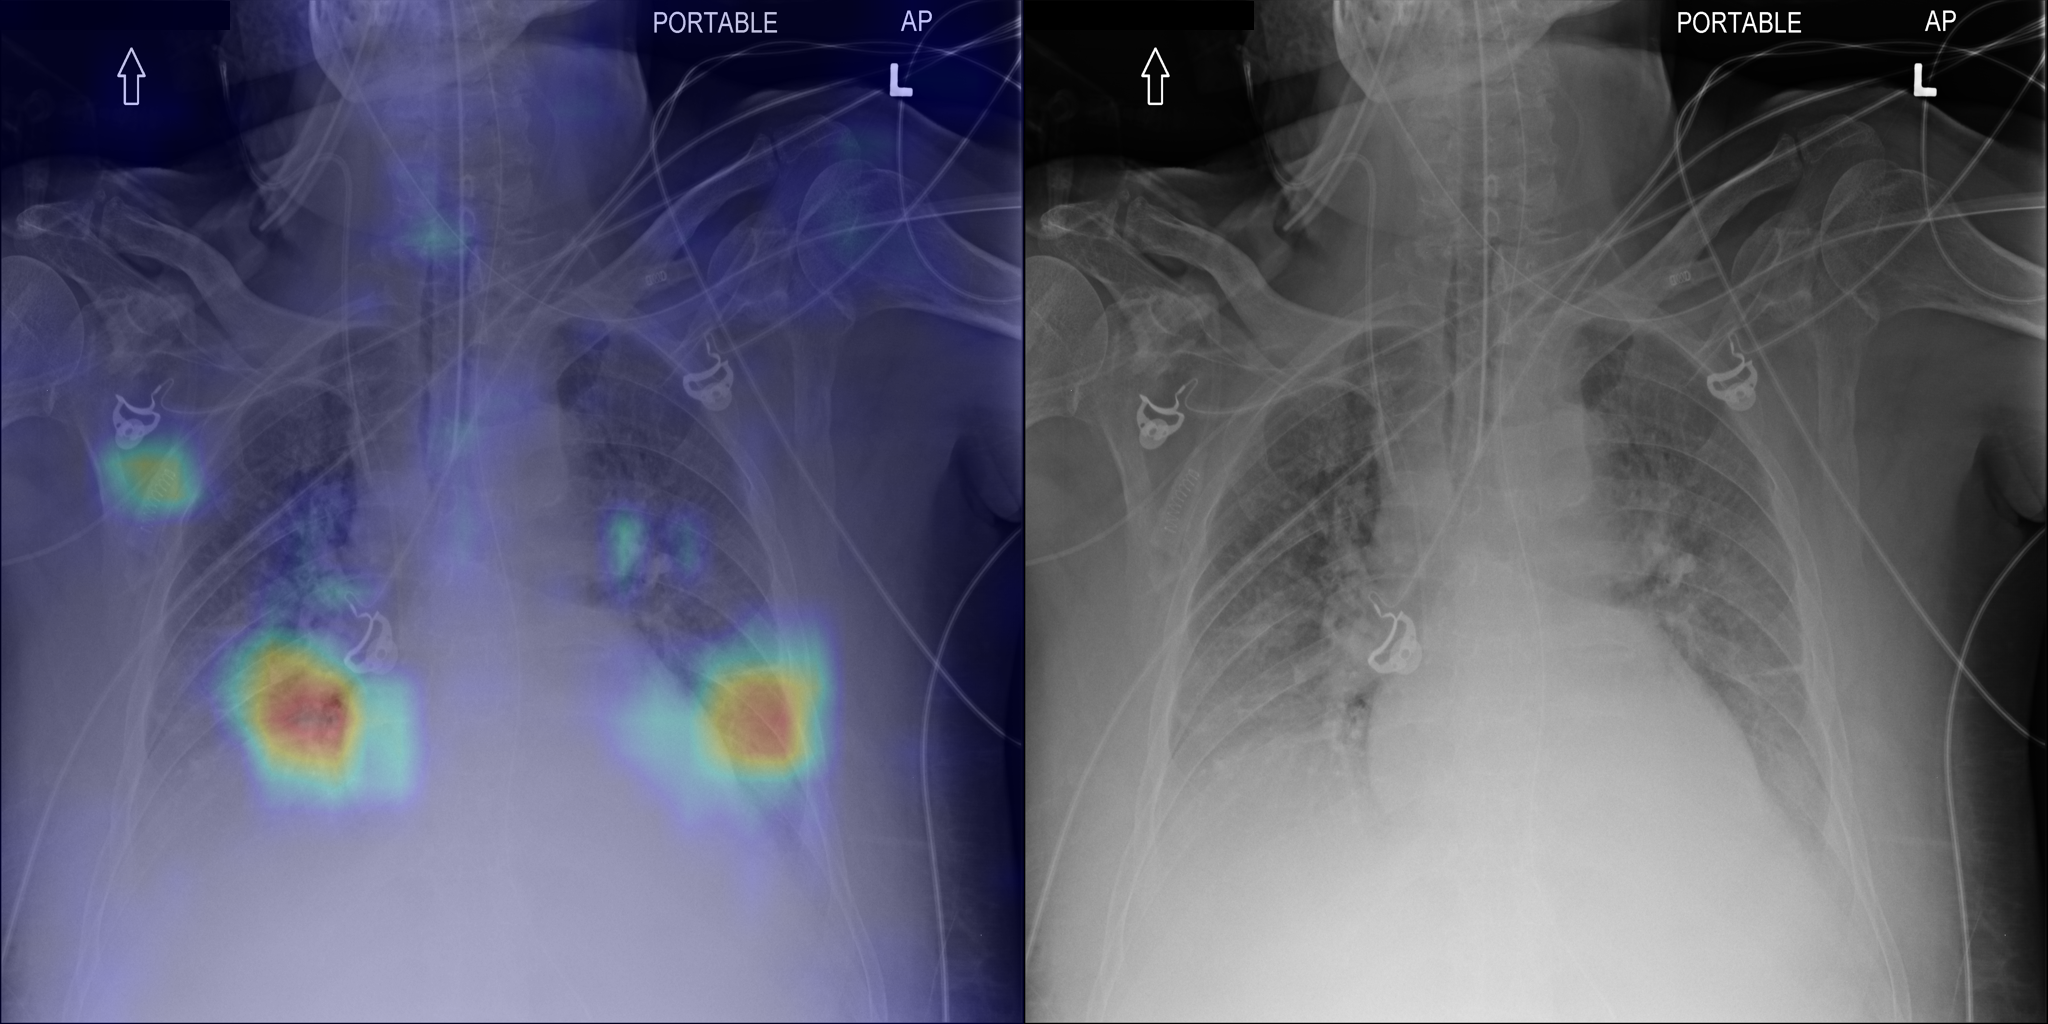
\includegraphics[width=1.0\textwidth]{Chapters/5. Conclusiones/img/Atelectasis/1_1_00030408_013.png}
    \end{subfigure}
    \begin{subfigure}{0.4\textwidth}
        \centering
        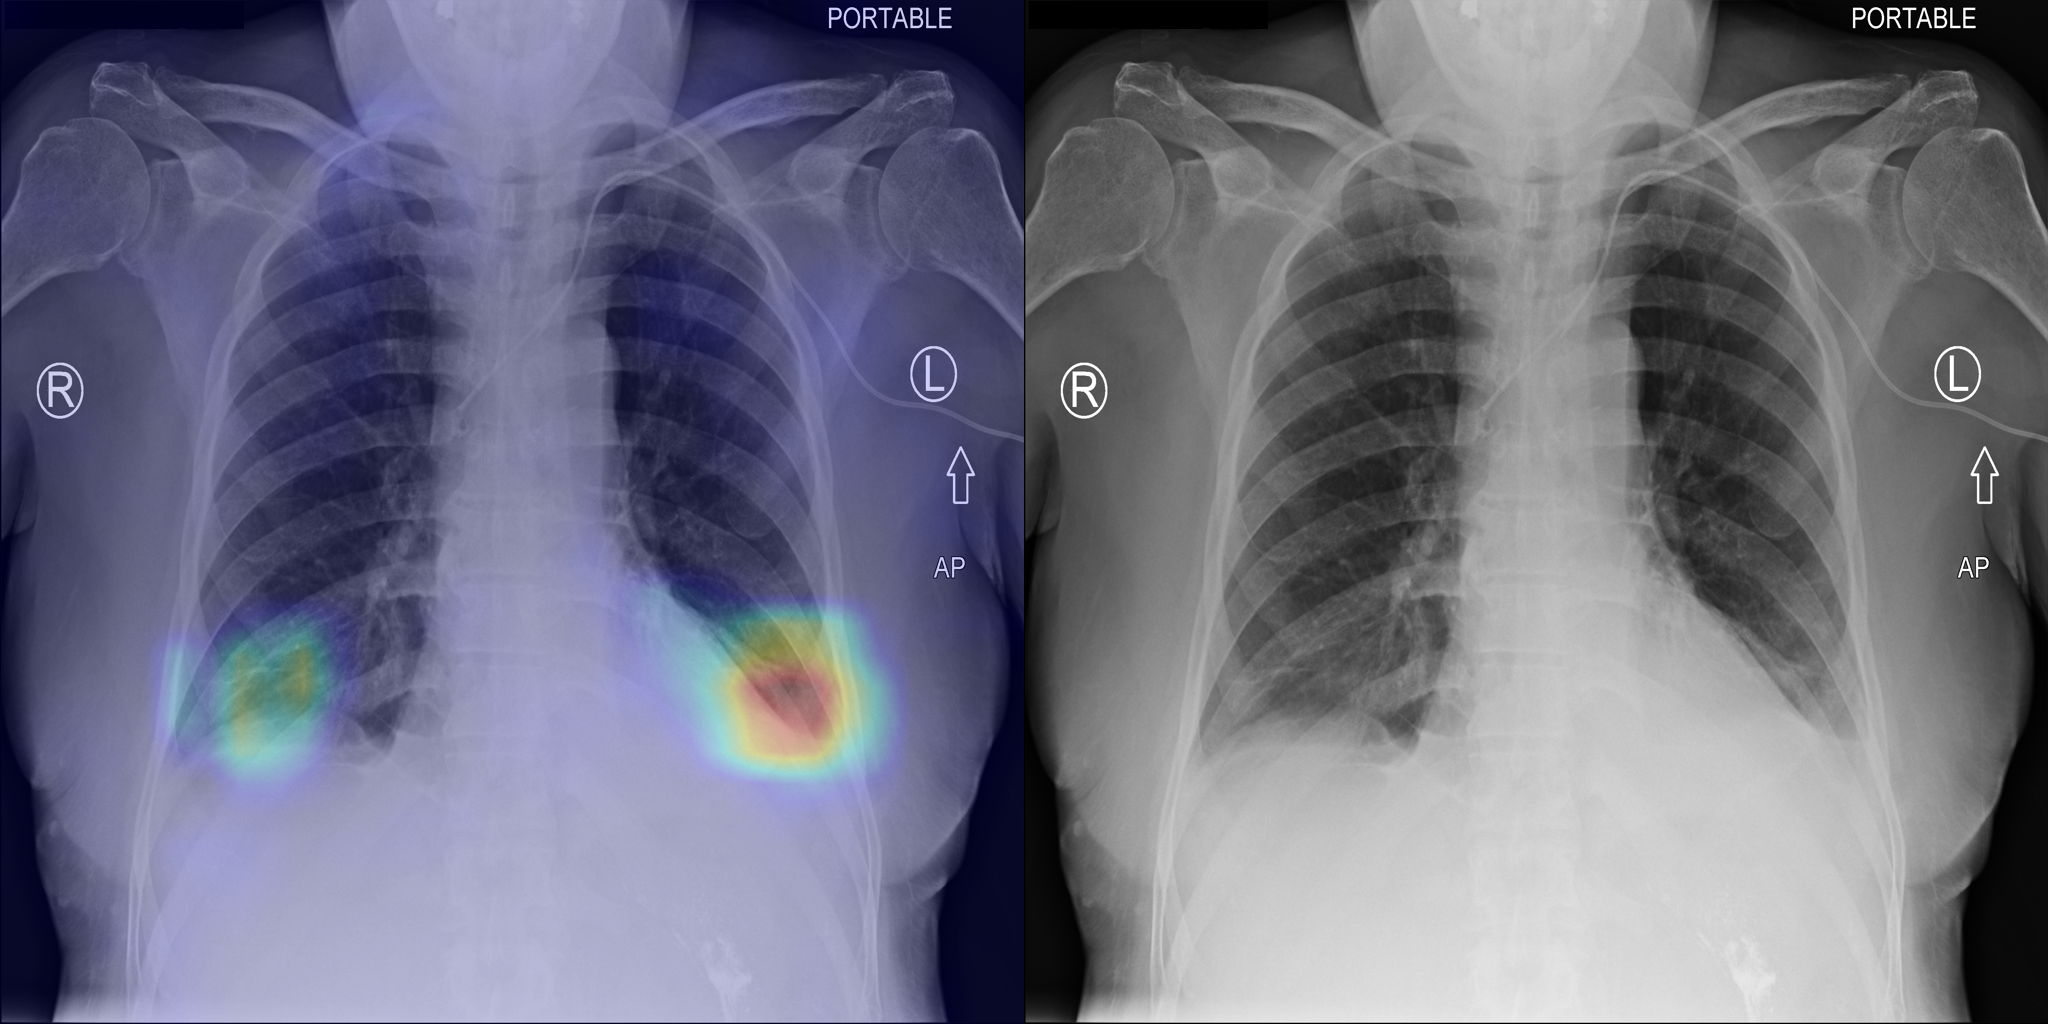
\includegraphics[width=1.0\textwidth]{Chapters/5. Conclusiones/img/Atelectasis/1_1_00028974_018.png}
    \end{subfigure}

    \caption[short]{Atelectasis. Radiografías detectadas con la patología de atelectasis por los
                    radiólogos. A la izquierda de cada imagen el GradCam correspondiente a la detección
                    de la patología como positivo por el modelo CNN.}
\end{figure}

\begin{figure}[b]
    \centering
    \begin{subfigure}{0.4\textwidth}
        \centering
        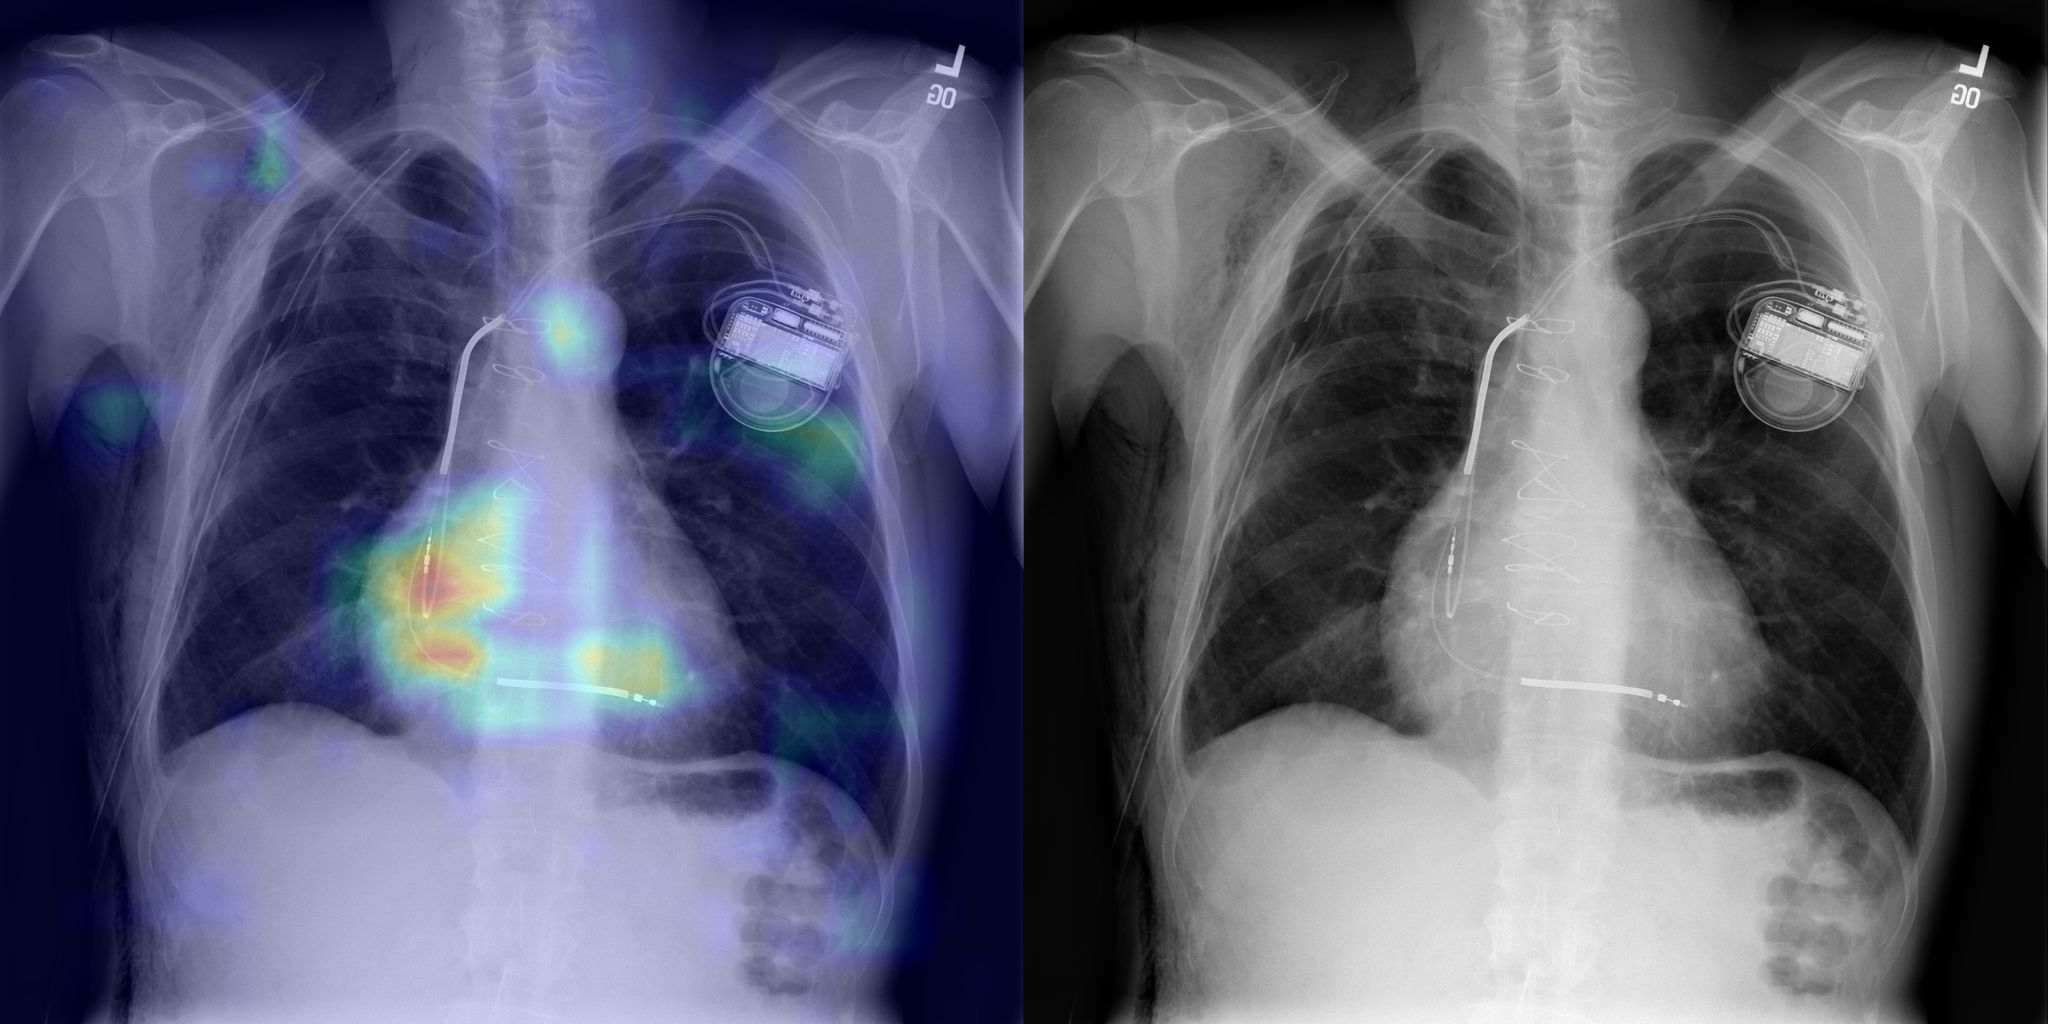
\includegraphics[width=1.0\textwidth]{Chapters/5. Conclusiones/img/Cardiomegaly/1_0_00000013_037.png}
    \end{subfigure}
    \begin{subfigure}{0.4\textwidth}
        \centering
        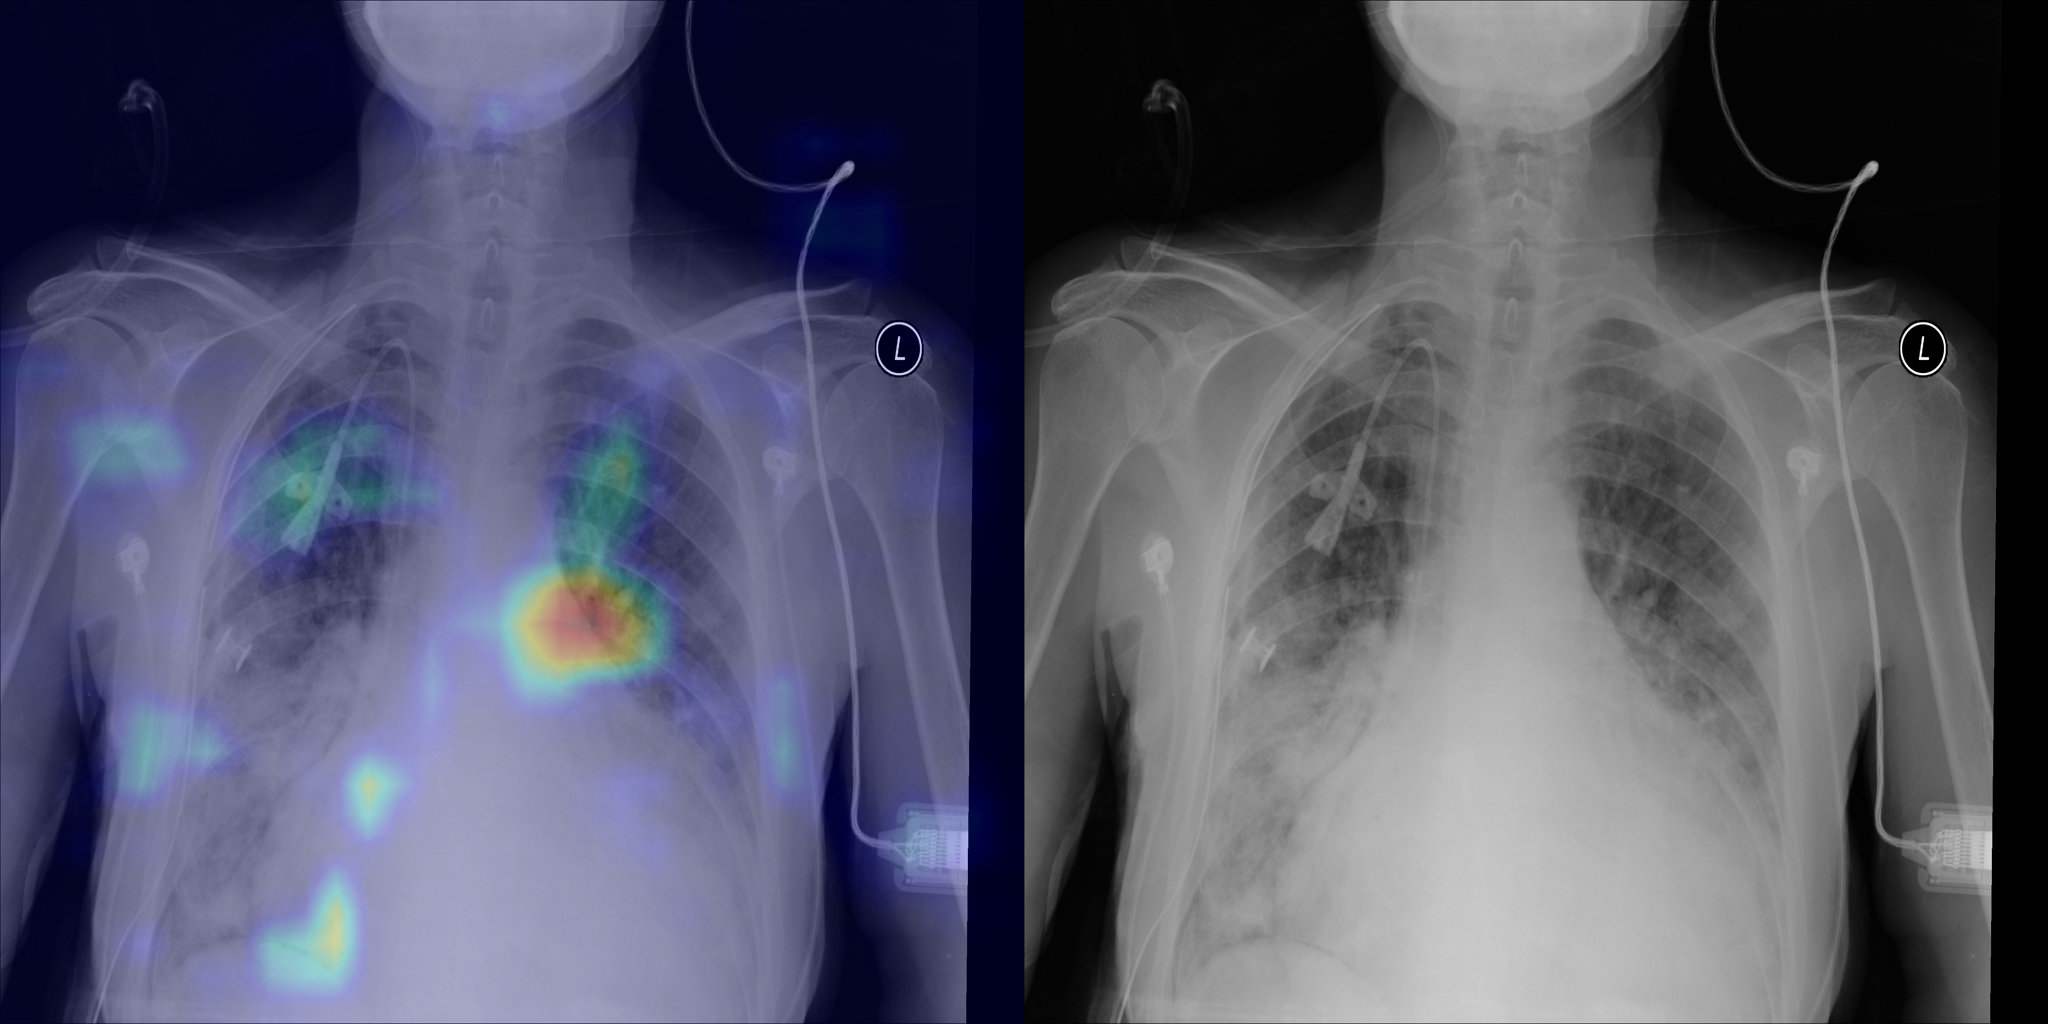
\includegraphics[width=1.0\textwidth]{Chapters/5. Conclusiones/img/Cardiomegaly/1_0_00000211_018.png}
    \end{subfigure}
    \begin{subfigure}{0.4\textwidth}
        \centering
        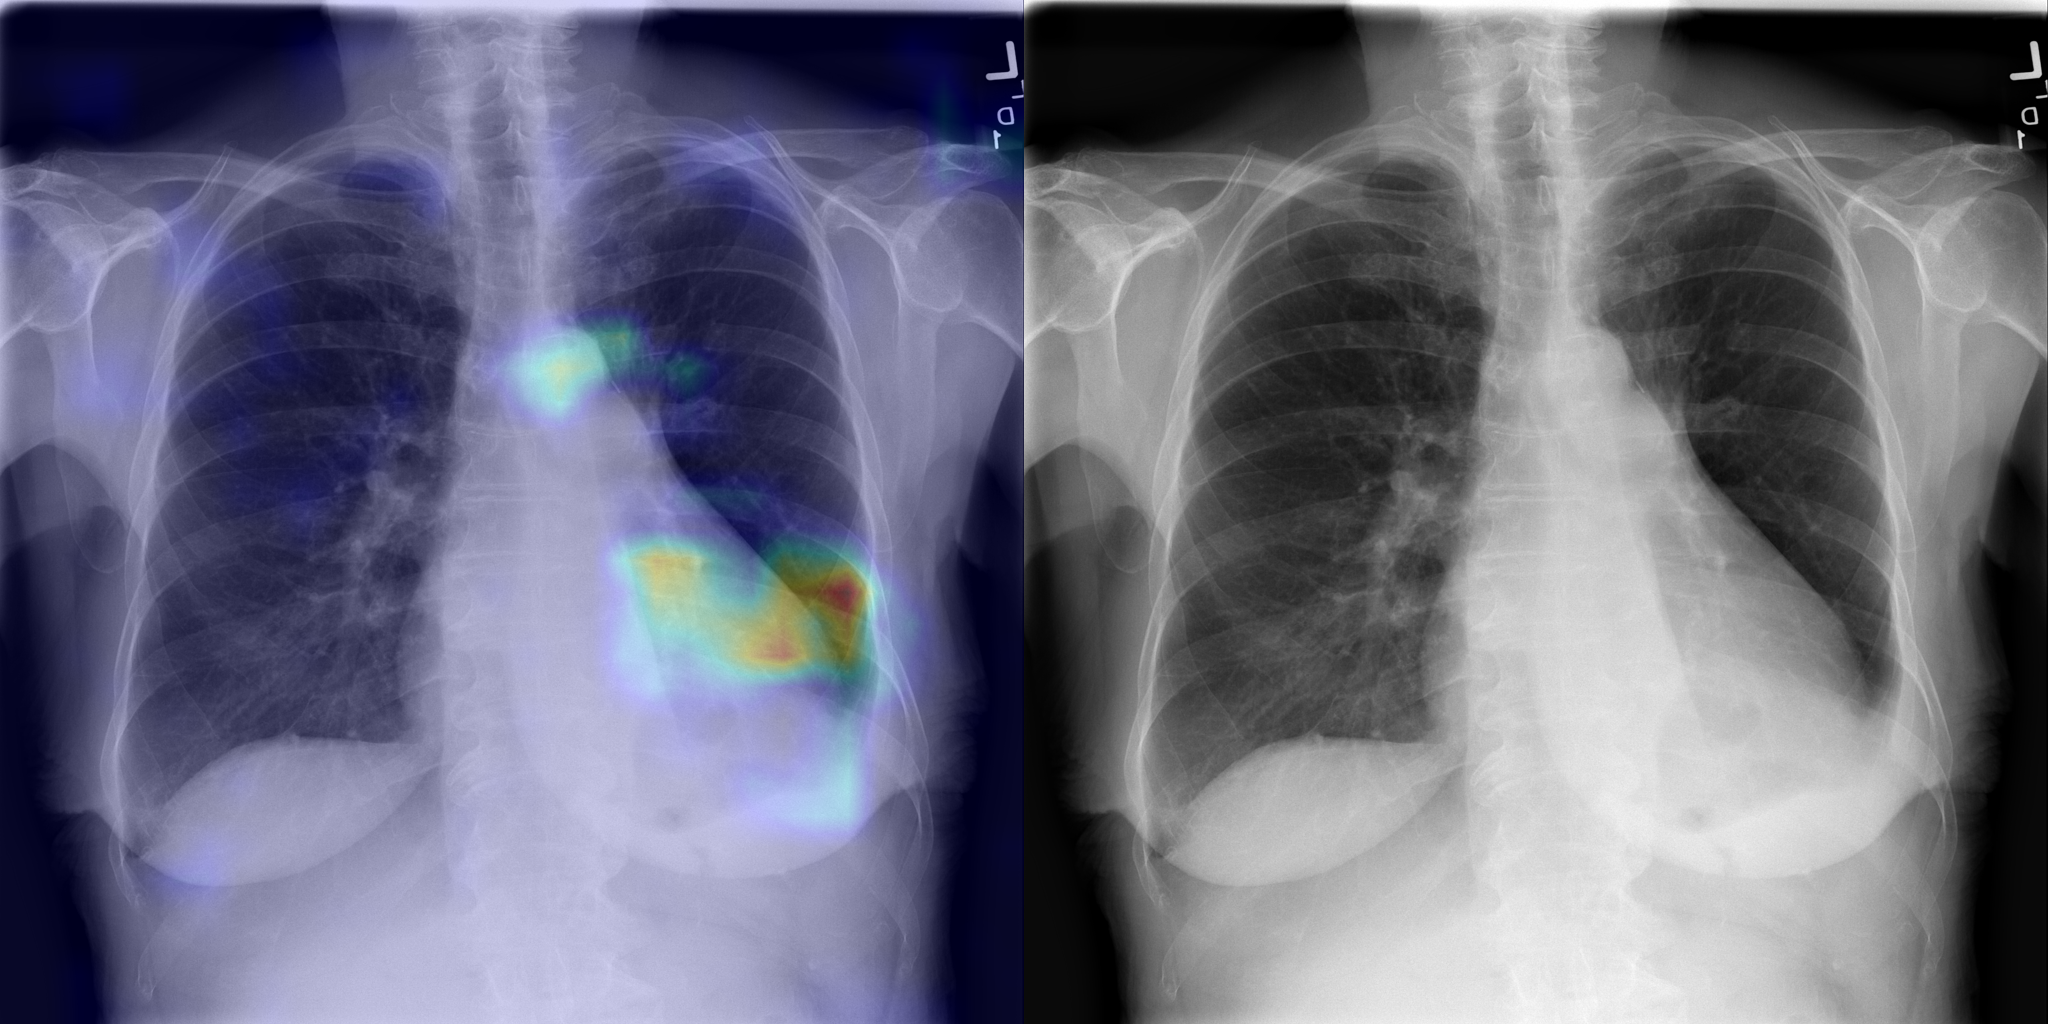
\includegraphics[width=1.0\textwidth]{Chapters/5. Conclusiones/img/Cardiomegaly/1_0_00000732_008.png}
    \end{subfigure}
    \begin{subfigure}{0.4\textwidth}
        \centering
        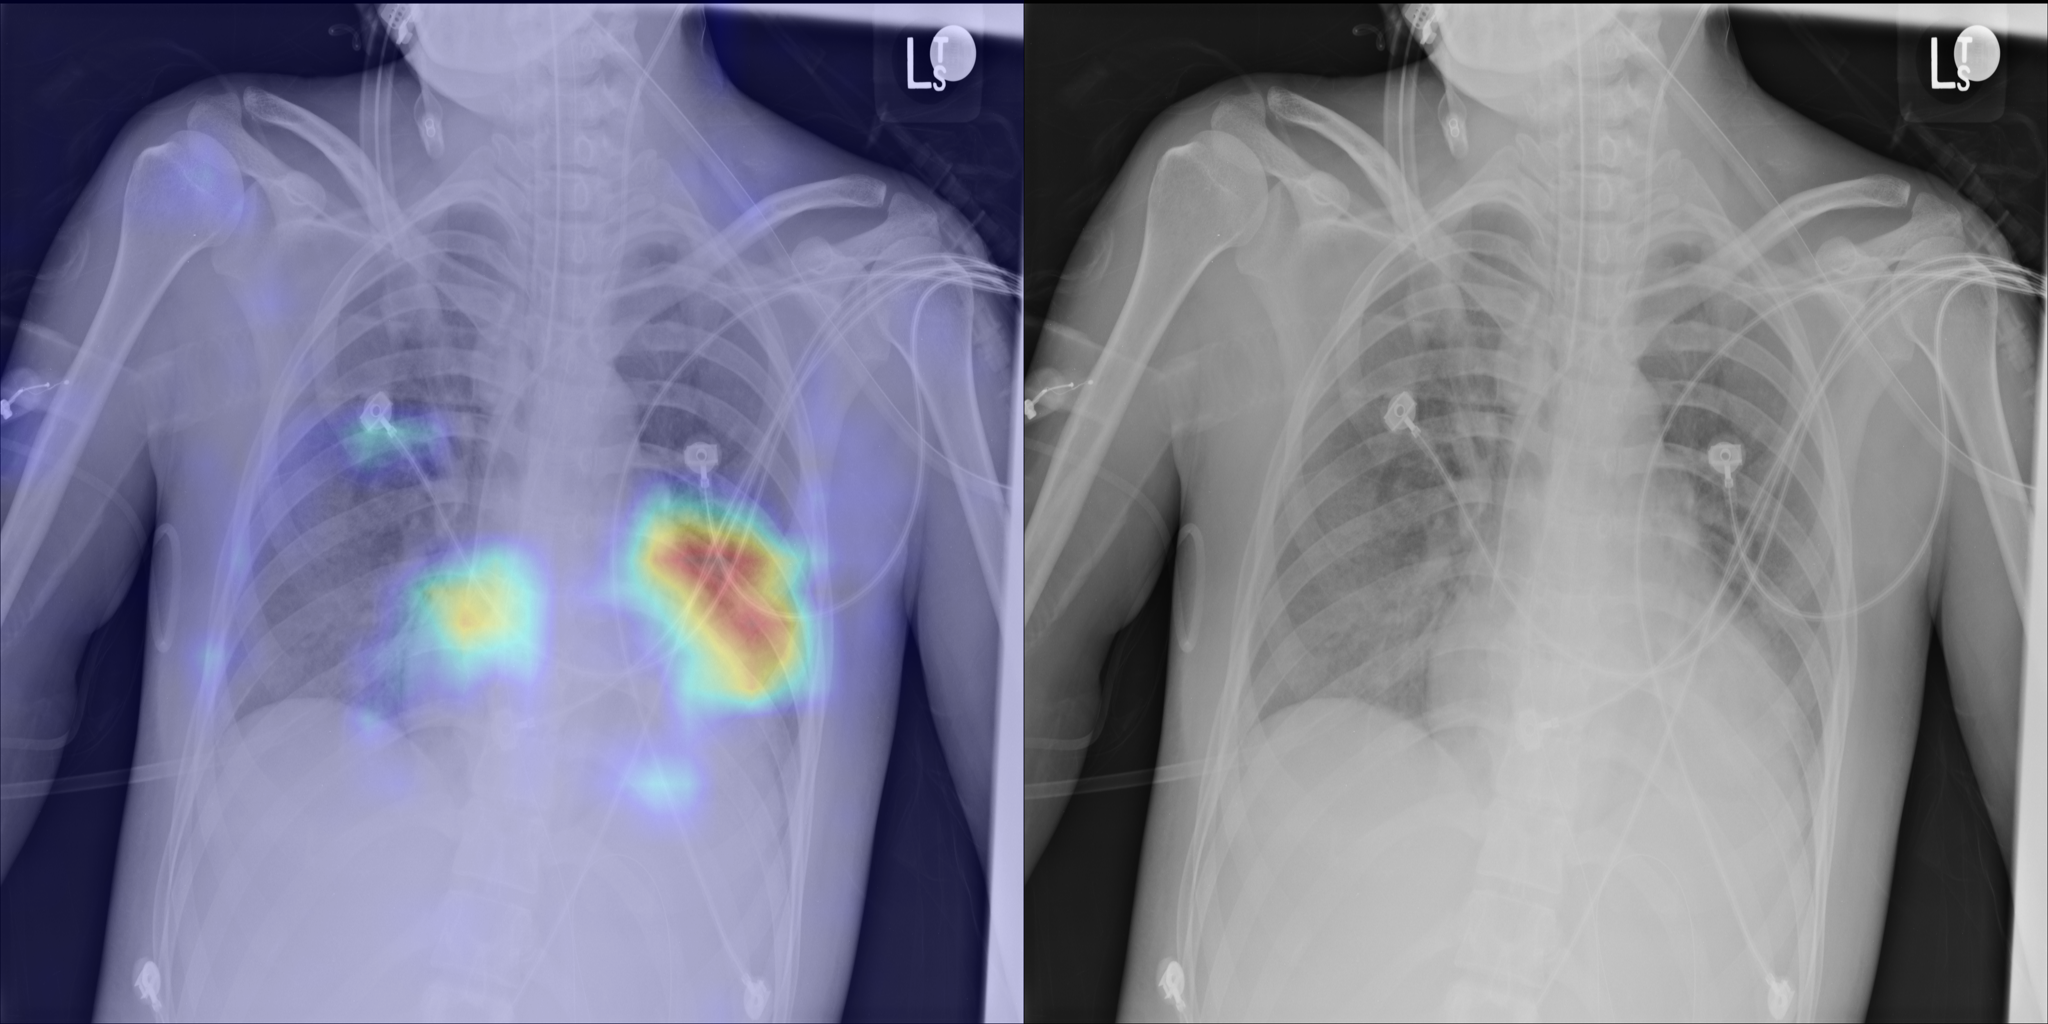
\includegraphics[width=1.0\textwidth]{Chapters/5. Conclusiones/img/Cardiomegaly/1_0_00001582_008.png}
    \end{subfigure}
    \begin{subfigure}{0.4\textwidth}
        \centering
        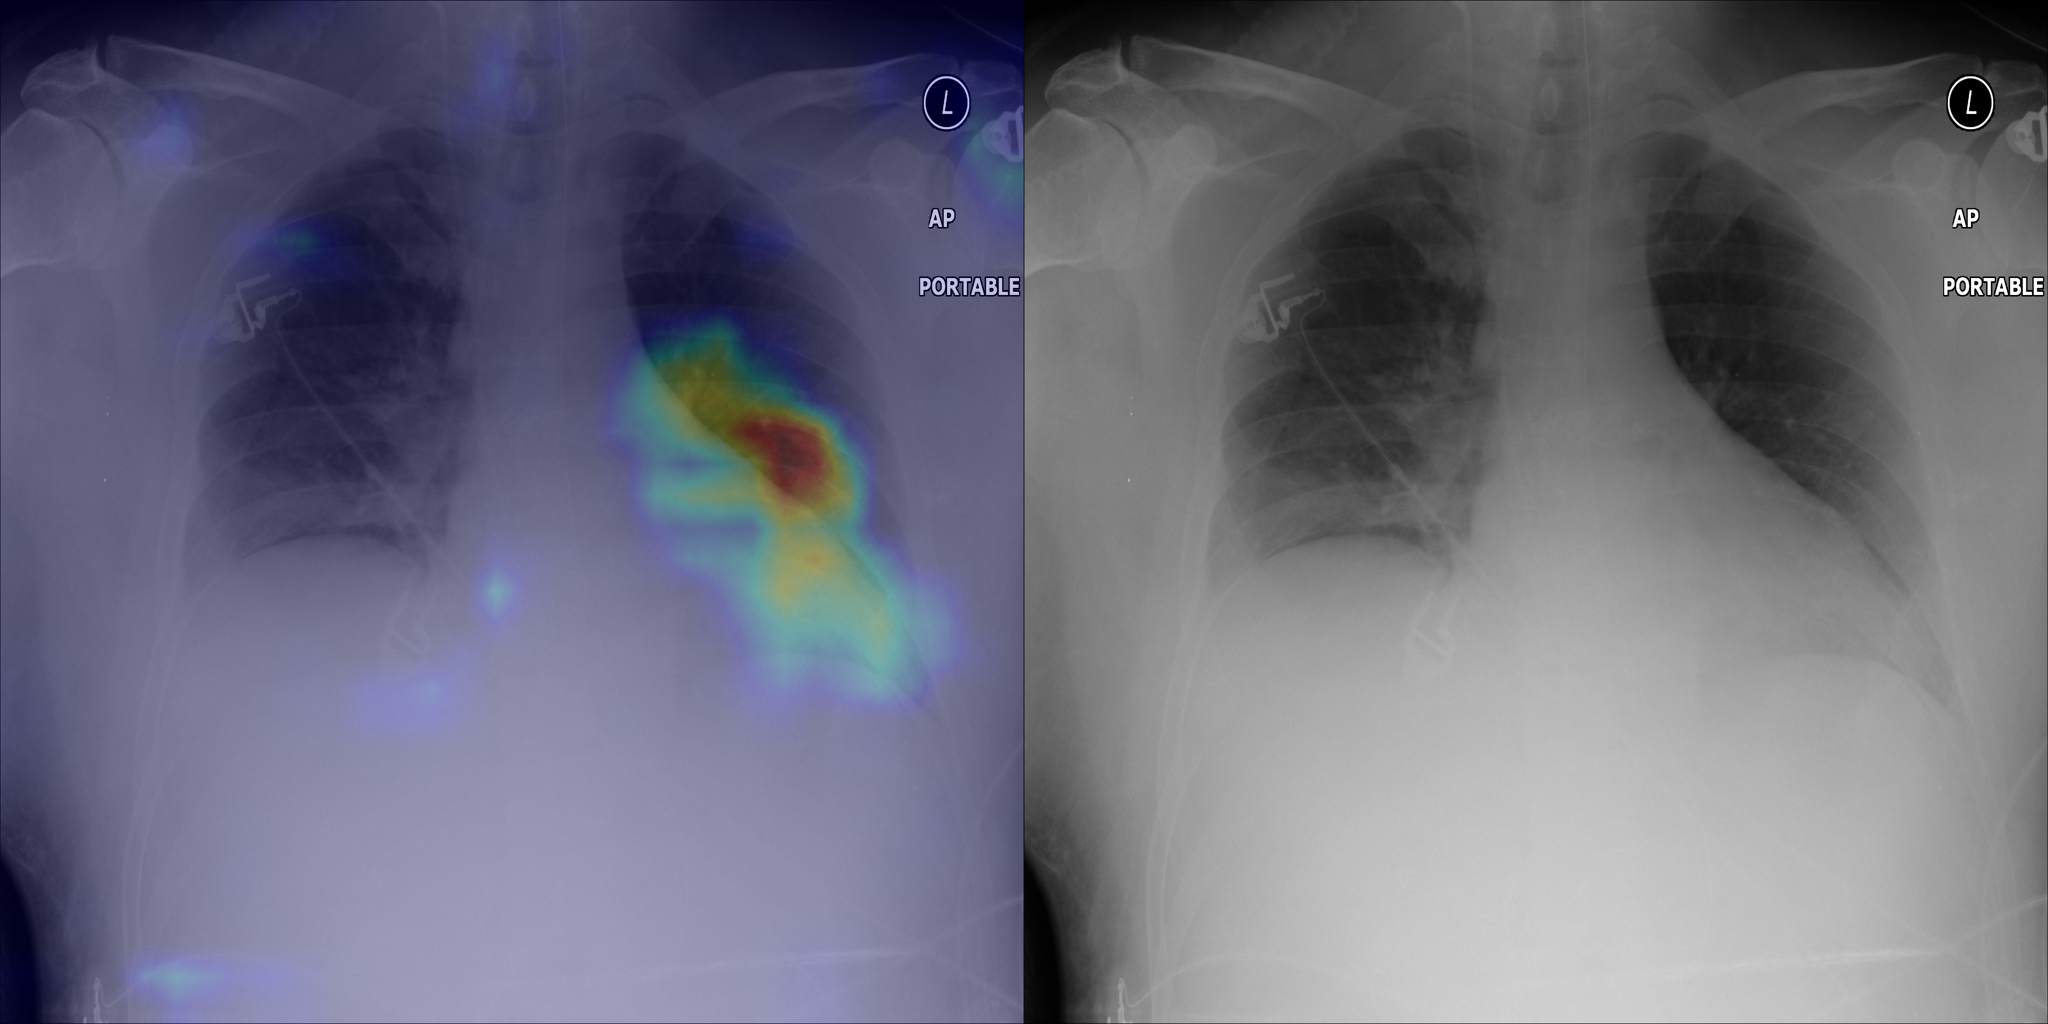
\includegraphics[width=1.0\textwidth]{Chapters/5. Conclusiones/img/Cardiomegaly/1_0_00002059_002.png}
    \end{subfigure}
    \begin{subfigure}{0.4\textwidth}
        \centering
        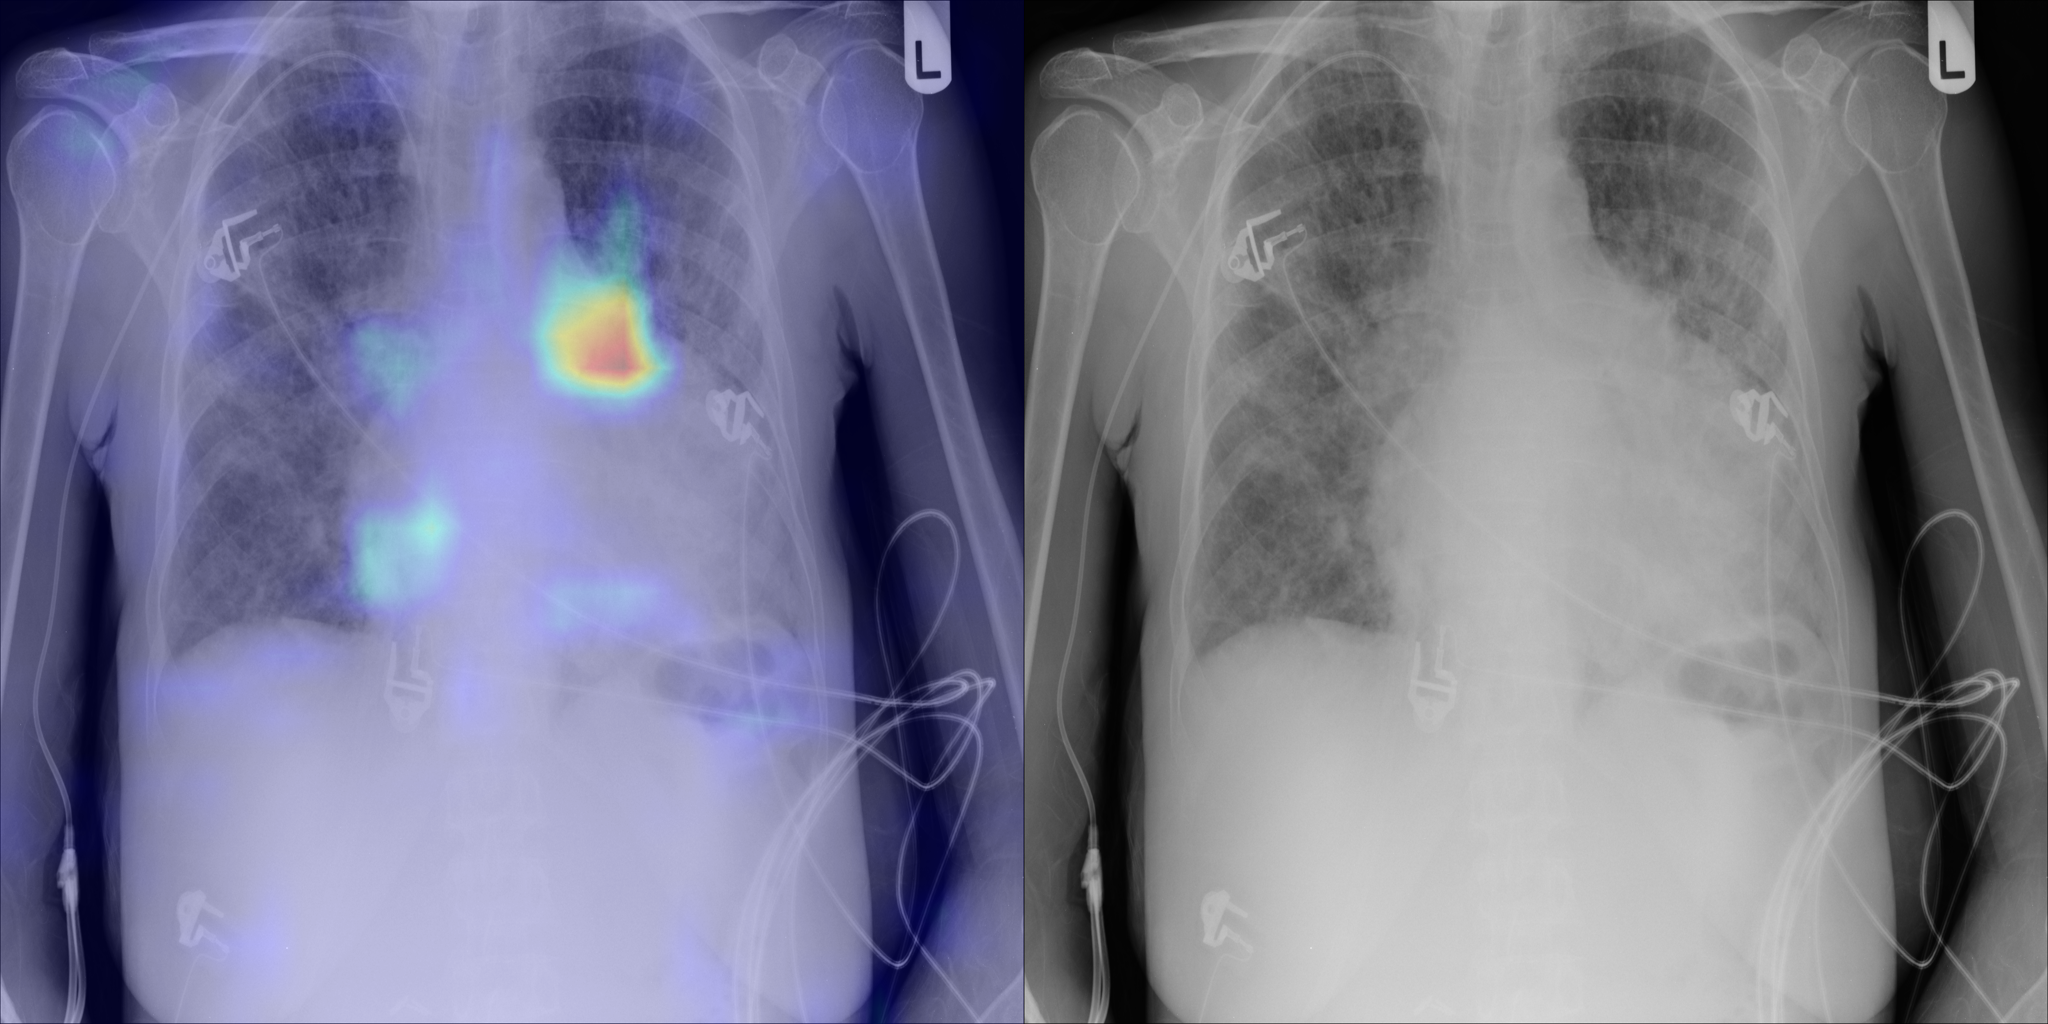
\includegraphics[width=1.0\textwidth]{Chapters/5. Conclusiones/img/Cardiomegaly/1_0_00004344_039.png}
    \end{subfigure}
    \begin{subfigure}{0.4\textwidth}
        \centering
        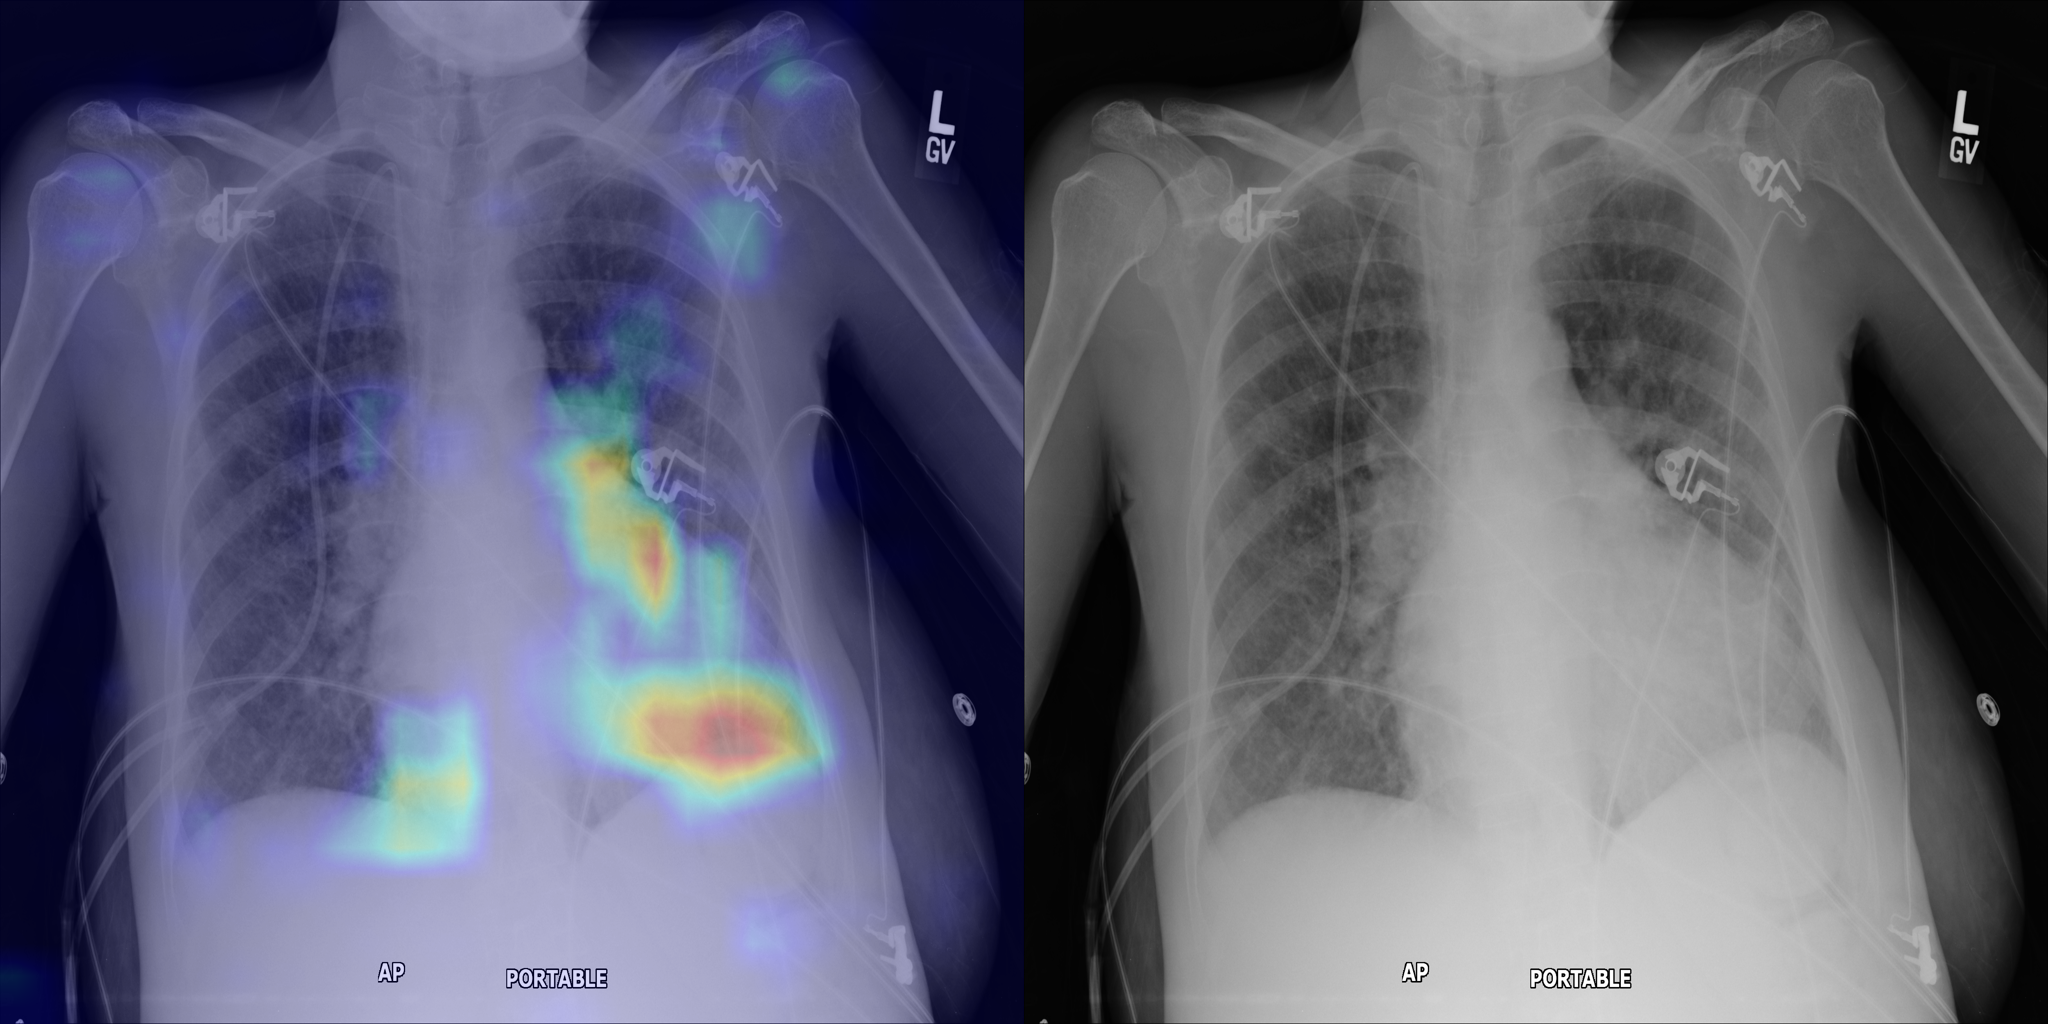
\includegraphics[width=1.0\textwidth]{Chapters/5. Conclusiones/img/Cardiomegaly/1_0_00004344_045.png}
    \end{subfigure}
    \begin{subfigure}{0.4\textwidth}
        \centering
        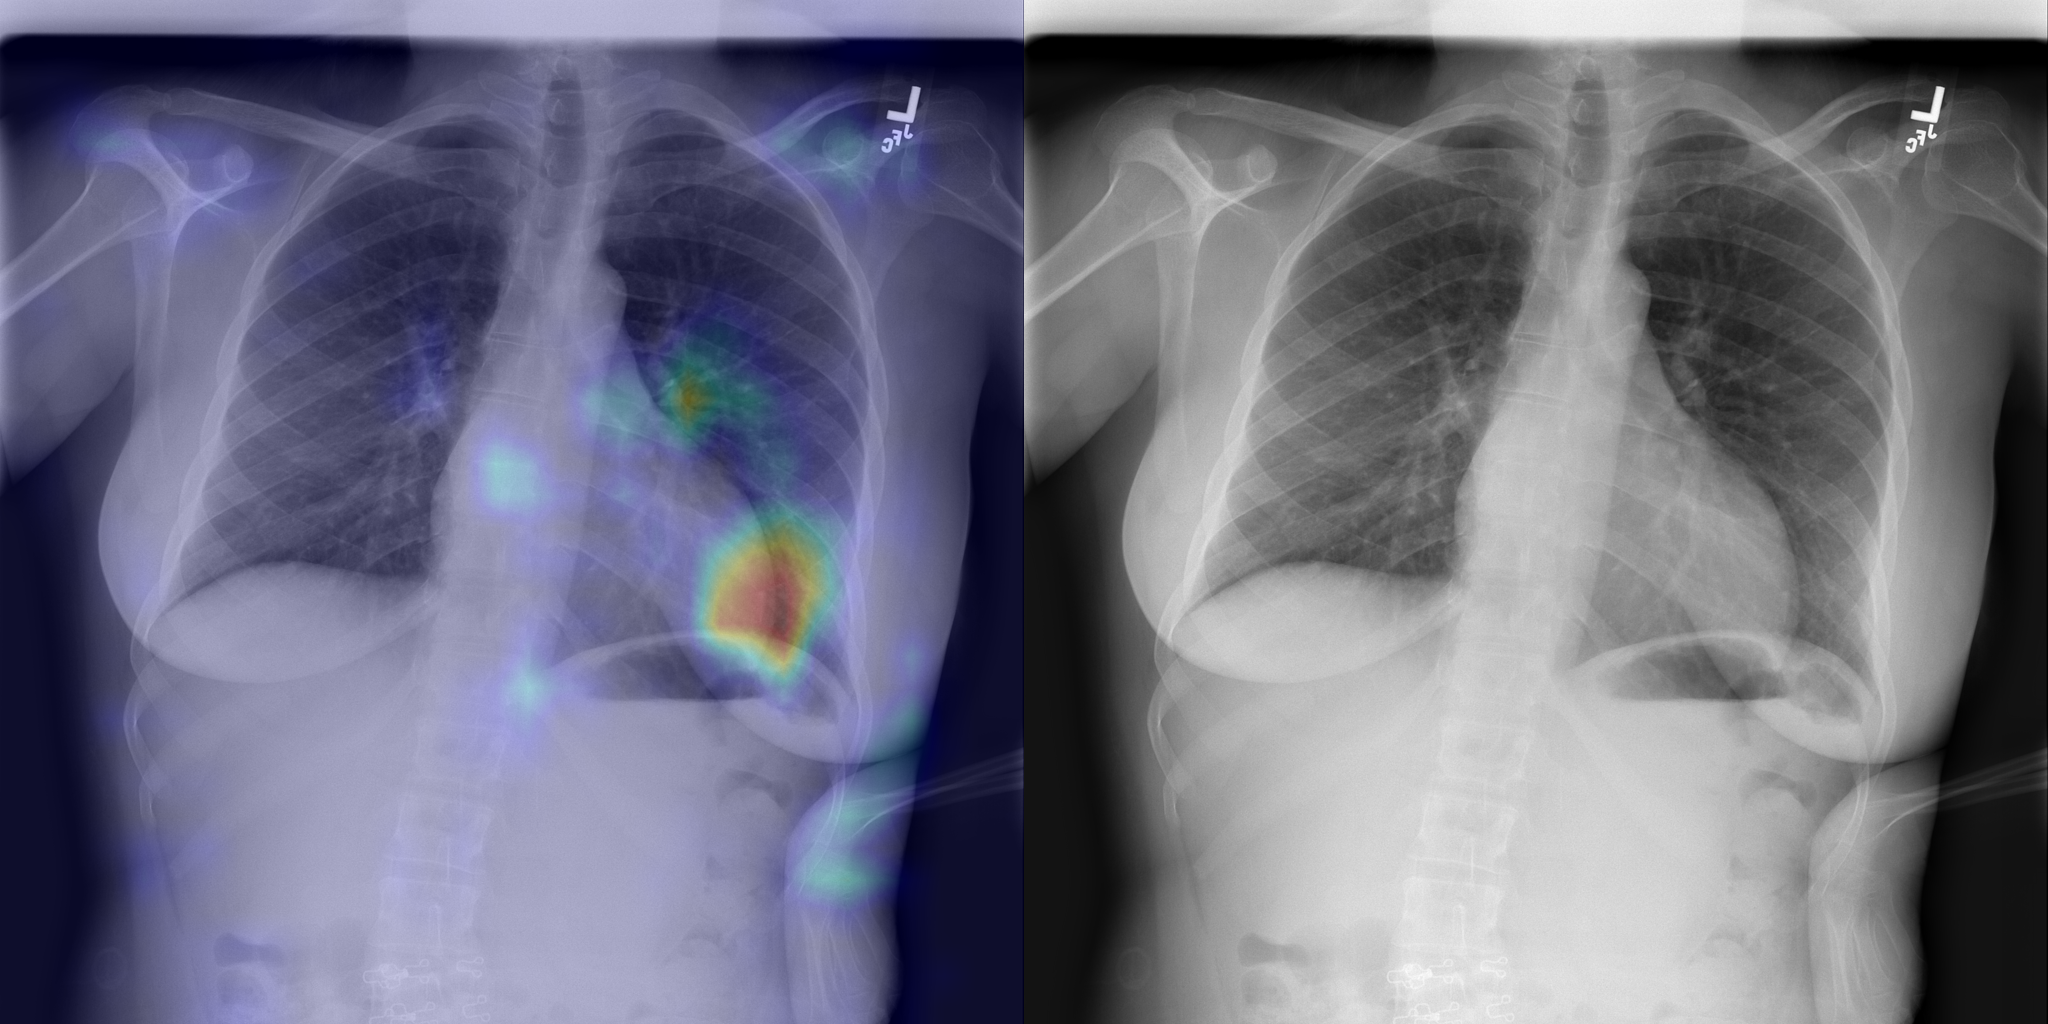
\includegraphics[width=1.0\textwidth]{Chapters/5. Conclusiones/img/Cardiomegaly/1_0_00004526_017.png}
    \end{subfigure}
    \begin{subfigure}{0.4\textwidth}
        \centering
        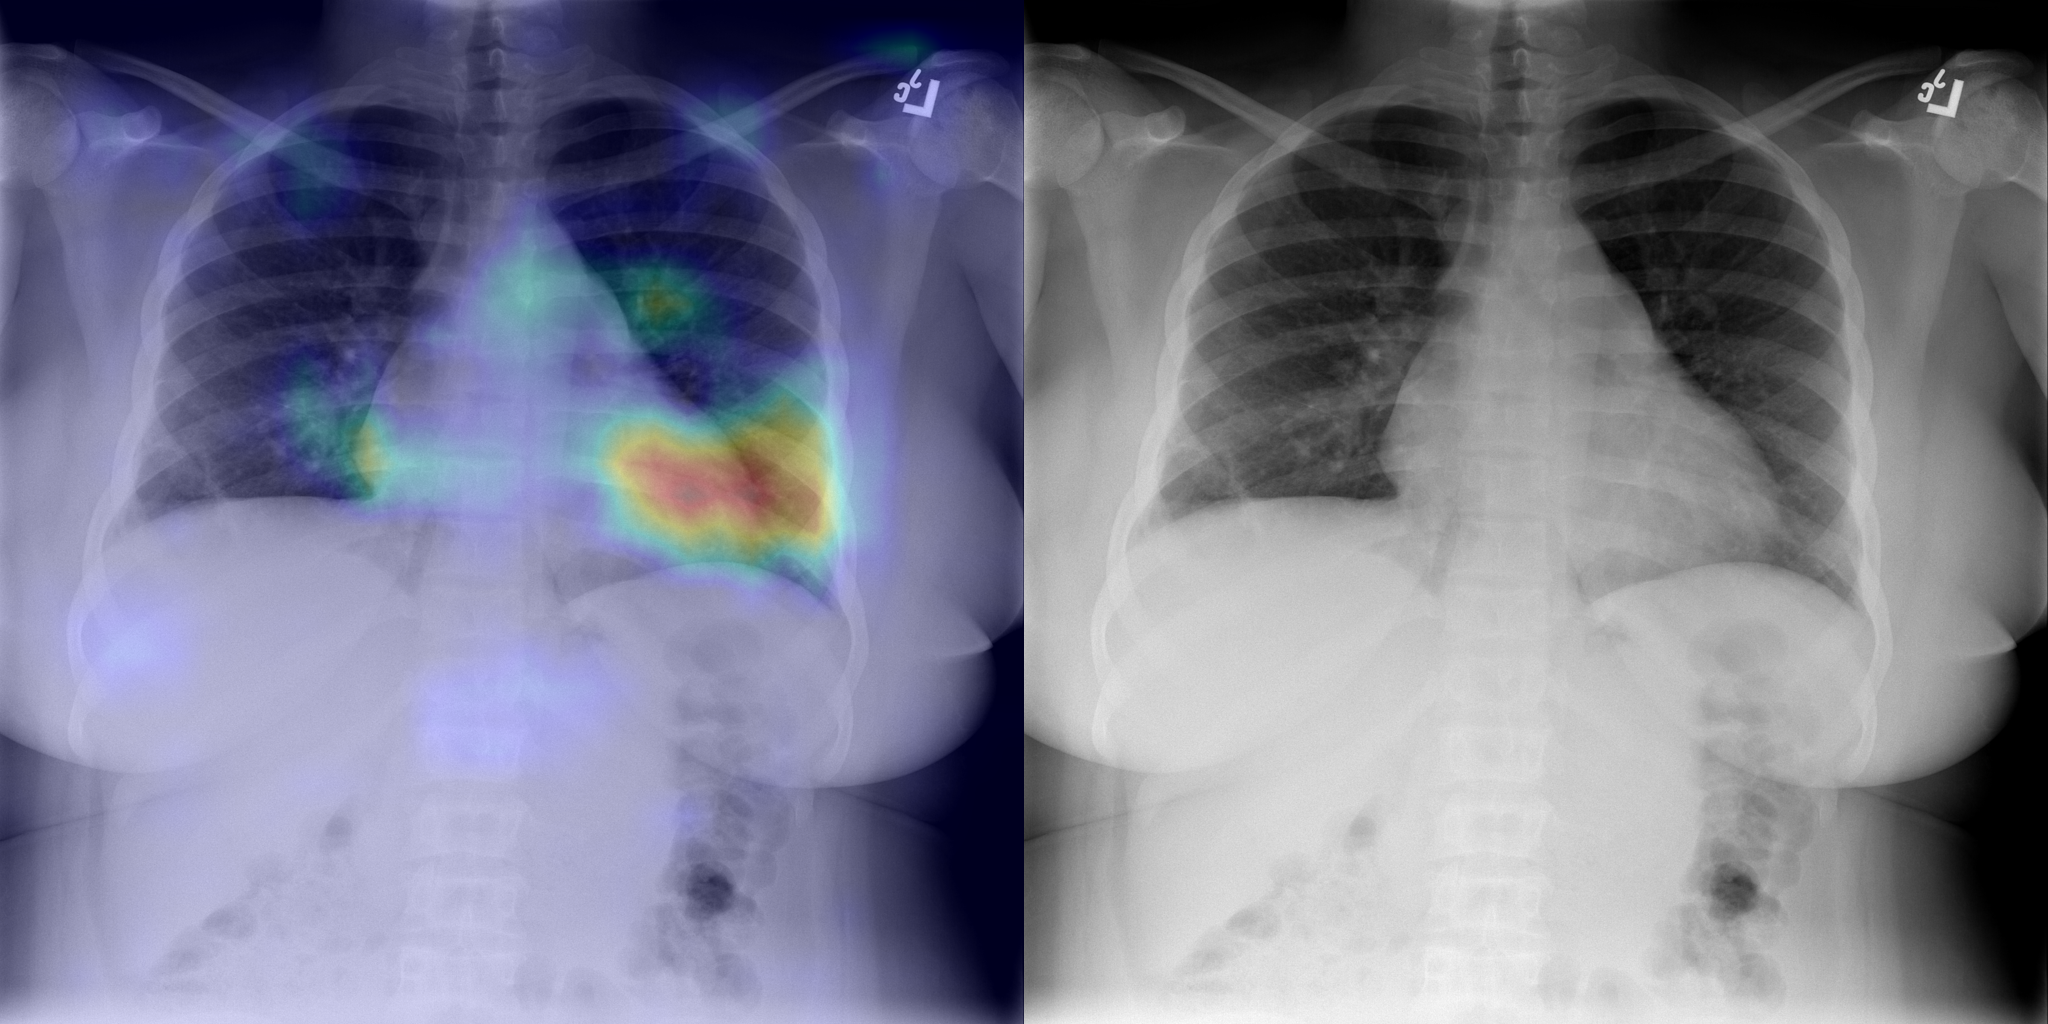
\includegraphics[width=1.0\textwidth]{Chapters/5. Conclusiones/img/Cardiomegaly/1_1_00014706_010.png}
    \end{subfigure}
    \begin{subfigure}{0.4\textwidth}
        \centering
        \includegraphics[width=1.0\textwidth]{Chapters/5. Conclusiones/img/Cardiomegaly/1_1_00016291_042.png}
    \end{subfigure}

    \caption[short]{Cardiomegalia. Radiografías detectadas con la patología de cardiomegalia por los
                    radiólogos. A la izquierda de cada imagen el GradCam correspondiente a la detección
                    de la patología como positivo por el modelo CNN.}
\end{figure}

\begin{figure}[b]
    \centering
    \begin{subfigure}{0.4\textwidth}
        \centering
        \includegraphics[width=1.0\textwidth]{Chapters/5. Conclusiones/img/Consolidation/1_1_00000246_014.png}
    \end{subfigure}
    \begin{subfigure}{0.4\textwidth}
        \centering
        \includegraphics[width=1.0\textwidth]{Chapters/5. Conclusiones/img/Consolidation/1_1_00000246_016.png}
    \end{subfigure}
    \begin{subfigure}{0.4\textwidth}
        \centering
        \includegraphics[width=1.0\textwidth]{Chapters/5. Conclusiones/img/Consolidation/1_1_00000344_000.png}
    \end{subfigure}
    \begin{subfigure}{0.4\textwidth}
        \centering
        \includegraphics[width=1.0\textwidth]{Chapters/5. Conclusiones/img/Consolidation/1_1_00000467_002.png}
    \end{subfigure}
    \begin{subfigure}{0.4\textwidth}
        \centering
        \includegraphics[width=1.0\textwidth]{Chapters/5. Conclusiones/img/Consolidation/1_1_00000467_003.png}
    \end{subfigure}
    \begin{subfigure}{0.4\textwidth}
        \centering
        \includegraphics[width=1.0\textwidth]{Chapters/5. Conclusiones/img/Consolidation/1_1_00000618_008.png}
    \end{subfigure}
    \begin{subfigure}{0.4\textwidth}
        \centering
        \includegraphics[width=1.0\textwidth]{Chapters/5. Conclusiones/img/Consolidation/1_1_00000618_011.png}
    \end{subfigure}
    \begin{subfigure}{0.4\textwidth}
        \centering
        \includegraphics[width=1.0\textwidth]{Chapters/5. Conclusiones/img/Consolidation/1_1_00000808_002.png}
    \end{subfigure}
    \begin{subfigure}{0.4\textwidth}
        \centering
        \includegraphics[width=1.0\textwidth]{Chapters/5. Conclusiones/img/Consolidation/1_1_00000882_003.png}
    \end{subfigure}
    \begin{subfigure}{0.4\textwidth}
        \centering
        \includegraphics[width=1.0\textwidth]{Chapters/5. Conclusiones/img/Consolidation/1_1_00018187_052.png}
    \end{subfigure}

    \caption[short]{Consolidación pulmunar. Radiografías detectadas con la patología de consolidación pulmunar por los
                    radiólogos. A la izquierda de cada imagen el GradCam correspondiente a la detección
                    de la patología como positivo por el modelo CNN.}
\end{figure}

\begin{figure}[b]
    \centering
    \begin{subfigure}{0.4\textwidth}
        \centering
        \includegraphics[width=1.0\textwidth]{Chapters/5. Conclusiones/img/COVID-19/1_1_0c9b15035c41_3ea703bd1e0b.png}
    \end{subfigure}
    \begin{subfigure}{0.4\textwidth}
        \centering
        \includegraphics[width=1.0\textwidth]{Chapters/5. Conclusiones/img/COVID-19/1_1_0d5082a9a044_d417f8e64511.png}
    \end{subfigure}
    \begin{subfigure}{0.4\textwidth}
        \centering
        \includegraphics[width=1.0\textwidth]{Chapters/5. Conclusiones/img/COVID-19/1_1_1b5ca94ac38b_68fcf433c6fe.png}
    \end{subfigure}
    \begin{subfigure}{0.4\textwidth}
        \centering
        \includegraphics[width=1.0\textwidth]{Chapters/5. Conclusiones/img/COVID-19/1_1_1b5ca94ac38b_0919a3b8af01.png}
    \end{subfigure}
    \begin{subfigure}{0.4\textwidth}
        \centering
        \includegraphics[width=1.0\textwidth]{Chapters/5. Conclusiones/img/COVID-19/1_1_1e3f6f8e494c_efe83e860c17.png}
    \end{subfigure}
    \begin{subfigure}{0.4\textwidth}
        \centering
        \includegraphics[width=1.0\textwidth]{Chapters/5. Conclusiones/img/COVID-19/1_1_4bb14a344446_0d3910133fbe.png}
    \end{subfigure}
    \begin{subfigure}{0.4\textwidth}
        \centering
        \includegraphics[width=1.0\textwidth]{Chapters/5. Conclusiones/img/COVID-19/1_1_4be426760e00_16d85c7f7837.png}
    \end{subfigure}
    \begin{subfigure}{0.4\textwidth}
        \centering
        \includegraphics[width=1.0\textwidth]{Chapters/5. Conclusiones/img/COVID-19/1_1_7b6c49da06db_b6b631939d4f.png}
    \end{subfigure}
    \begin{subfigure}{0.4\textwidth}
        \centering
        \includegraphics[width=1.0\textwidth]{Chapters/5. Conclusiones/img/COVID-19/1_1_cde0ab9526da_fa935d855d4e.png}
    \end{subfigure}
    \begin{subfigure}{0.4\textwidth}
        \centering
        \includegraphics[width=1.0\textwidth]{Chapters/5. Conclusiones/img/COVID-19/1_1_covid-19-pneumonia-20-pa-on-admission.jpg}
    \end{subfigure}

    \caption[short]{Covid-19. Radiografías detectadas con la patología de Covid-19 por los
                    radiólogos. A la izquierda de cada imagen el GradCam correspondiente a la detección
                    de la patología como positivo por el modelo CNN.}
\end{figure}

\begin{figure}[b]
    \centering
    \begin{subfigure}{0.4\textwidth}
        \centering
        \includegraphics[width=1.0\textwidth]{Chapters/5. Conclusiones/img/Edema/1_1_00001373_031.png}
    \end{subfigure}
    \begin{subfigure}{0.4\textwidth}
        \centering
        \includegraphics[width=1.0\textwidth]{Chapters/5. Conclusiones/img/Edema/1_1_00001373_032.png}
    \end{subfigure}
    \begin{subfigure}{0.4\textwidth}
        \centering
        \includegraphics[width=1.0\textwidth]{Chapters/5. Conclusiones/img/Edema/1_1_00001787_000.png}
    \end{subfigure}
    \begin{subfigure}{0.4\textwidth}
        \centering
        \includegraphics[width=1.0\textwidth]{Chapters/5. Conclusiones/img/Edema/1_1_00003528_021.png}
    \end{subfigure}
    \begin{subfigure}{0.4\textwidth}
        \centering
        \includegraphics[width=1.0\textwidth]{Chapters/5. Conclusiones/img/Edema/1_1_00003803_009.png}
    \end{subfigure}
    \begin{subfigure}{0.4\textwidth}
        \centering
        \includegraphics[width=1.0\textwidth]{Chapters/5. Conclusiones/img/Edema/1_1_00004533_020.png}
    \end{subfigure}
    \begin{subfigure}{0.4\textwidth}
        \centering
        \includegraphics[width=1.0\textwidth]{Chapters/5. Conclusiones/img/Edema/1_1_00006304_002.png}
    \end{subfigure}
    \begin{subfigure}{0.4\textwidth}
        \centering
        \includegraphics[width=1.0\textwidth]{Chapters/5. Conclusiones/img/Edema/1_1_00006304_006.png}
    \end{subfigure}
    \begin{subfigure}{0.4\textwidth}
        \centering
        \includegraphics[width=1.0\textwidth]{Chapters/5. Conclusiones/img/Edema/1_1_00010535_002.png}
    \end{subfigure}
    \begin{subfigure}{0.4\textwidth}
        \centering
        \includegraphics[width=1.0\textwidth]{Chapters/5. Conclusiones/img/Edema/1_1_00011583_006.png}
    \end{subfigure}

    \caption[short]{Edema. Radiografías detectadas con la patología de edema pulmonar por los
                    radiólogos. A la izquierda de cada imagen el GradCam correspondiente a la detección
                    de la patología como positivo por el modelo CNN.}
\end{figure}

\begin{figure}[b]
    \centering
    \begin{subfigure}{0.4\textwidth}
        \centering
        \includegraphics[width=1.0\textwidth]{Chapters/5. Conclusiones/img/Effusion/1_1_00000092_001.png}
    \end{subfigure}
    \begin{subfigure}{0.4\textwidth}
        \centering
        \includegraphics[width=1.0\textwidth]{Chapters/5. Conclusiones/img/Effusion/1_1_00000147_002.png}
    \end{subfigure}
    \begin{subfigure}{0.4\textwidth}
        \centering
        \includegraphics[width=1.0\textwidth]{Chapters/5. Conclusiones/img/Effusion/1_1_00000181_005.png}
    \end{subfigure}
    \begin{subfigure}{0.4\textwidth}
        \centering
        \includegraphics[width=1.0\textwidth]{Chapters/5. Conclusiones/img/Effusion/1_1_00000181_054.png}
    \end{subfigure}
    \begin{subfigure}{0.4\textwidth}
        \centering
        \includegraphics[width=1.0\textwidth]{Chapters/5. Conclusiones/img/Effusion/1_1_00000181_055.png}
    \end{subfigure}
    \begin{subfigure}{0.4\textwidth}
        \centering
        \includegraphics[width=1.0\textwidth]{Chapters/5. Conclusiones/img/Effusion/1_1_00000211_004.png}
    \end{subfigure}
    \begin{subfigure}{0.4\textwidth}
        \centering
        \includegraphics[width=1.0\textwidth]{Chapters/5. Conclusiones/img/Effusion/1_1_00000211_008.png}
    \end{subfigure}
    \begin{subfigure}{0.4\textwidth}
        \centering
        \includegraphics[width=1.0\textwidth]{Chapters/5. Conclusiones/img/Effusion/1_1_00000211_011.png}
    \end{subfigure}
    \begin{subfigure}{0.4\textwidth}
        \centering
        \includegraphics[width=1.0\textwidth]{Chapters/5. Conclusiones/img/Effusion/1_1_00022883_011.png}
    \end{subfigure}
    \begin{subfigure}{0.4\textwidth}
        \centering
        \includegraphics[width=1.0\textwidth]{Chapters/5. Conclusiones/img/Effusion/1_1_00022899_009.png}
    \end{subfigure}

    \caption[short]{Derrame pleural. Radiografías detectadas con la patología de derrame pleural por los
                    radiólogos. A la izquierda de cada imagen el GradCam correspondiente a la detección
                    de la patología como positivo por el modelo CNN.}
\end{figure}

\begin{figure}[b]
    \centering
    \begin{subfigure}{0.4\textwidth}
        \centering
        \includegraphics[width=1.0\textwidth]{Chapters/5. Conclusiones/img/Emphysema/1_1_00000312_001.png}
    \end{subfigure}
    \begin{subfigure}{0.4\textwidth}
        \centering
        \includegraphics[width=1.0\textwidth]{Chapters/5. Conclusiones/img/Emphysema/1_1_00000732_006.png}
    \end{subfigure}
    \begin{subfigure}{0.4\textwidth}
        \centering
        \includegraphics[width=1.0\textwidth]{Chapters/5. Conclusiones/img/Emphysema/1_1_00001093_000.png}
    \end{subfigure}
    \begin{subfigure}{0.4\textwidth}
        \centering
        \includegraphics[width=1.0\textwidth]{Chapters/5. Conclusiones/img/Emphysema/1_1_00001555_000.png}
    \end{subfigure}
    \begin{subfigure}{0.4\textwidth}
        \centering
        \includegraphics[width=1.0\textwidth]{Chapters/5. Conclusiones/img/Emphysema/1_1_00008841_062.png}
    \end{subfigure}
    \begin{subfigure}{0.4\textwidth}
        \centering
        \includegraphics[width=1.0\textwidth]{Chapters/5. Conclusiones/img/Emphysema/1_1_00011683_042.png}
    \end{subfigure}
    \begin{subfigure}{0.4\textwidth}
        \centering
        \includegraphics[width=1.0\textwidth]{Chapters/5. Conclusiones/img/Emphysema/1_1_00012298_007.png}
    \end{subfigure}
    \begin{subfigure}{0.4\textwidth}
        \centering
        \includegraphics[width=1.0\textwidth]{Chapters/5. Conclusiones/img/Emphysema/1_1_00015387_000.png}
    \end{subfigure}
    \begin{subfigure}{0.4\textwidth}
        \centering
        \includegraphics[width=1.0\textwidth]{Chapters/5. Conclusiones/img/Emphysema/1_1_00023075_007.png}
    \end{subfigure}
    \begin{subfigure}{0.4\textwidth}
        \centering
        \includegraphics[width=1.0\textwidth]{Chapters/5. Conclusiones/img/Emphysema/1_1_00023078_006.png}
    \end{subfigure}

    \caption[short]{Enfisema pulmonar. Radiografías detectadas con la patología de enfisema pulmonar por los
                    radiólogos. A la izquierda de cada imagen el GradCam correspondiente a la detección
                    de la patología como positivo por el modelo CNN.}
\end{figure}

\begin{figure}[b]
    \centering
    \begin{subfigure}{0.4\textwidth}
        \centering
        \includegraphics[width=1.0\textwidth]{Chapters/5. Conclusiones/img/Fibrosis/1_1_00000092_003.png}
    \end{subfigure}
    \begin{subfigure}{0.4\textwidth}
        \centering
        \includegraphics[width=1.0\textwidth]{Chapters/5. Conclusiones/img/Fibrosis/1_1_00000181_052.png}
    \end{subfigure}
    \begin{subfigure}{0.4\textwidth}
        \centering
        \includegraphics[width=1.0\textwidth]{Chapters/5. Conclusiones/img/Fibrosis/1_1_00000733_003.png}
    \end{subfigure}
    \begin{subfigure}{0.4\textwidth}
        \centering
        \includegraphics[width=1.0\textwidth]{Chapters/5. Conclusiones/img/Fibrosis/1_1_00001170_049.png}
    \end{subfigure}
    \begin{subfigure}{0.4\textwidth}
        \centering
        \includegraphics[width=1.0\textwidth]{Chapters/5. Conclusiones/img/Fibrosis/1_1_00003089_002.png}
    \end{subfigure}
    \begin{subfigure}{0.4\textwidth}
        \centering
        \includegraphics[width=1.0\textwidth]{Chapters/5. Conclusiones/img/Fibrosis/1_1_00003996_011.png}
    \end{subfigure}
    \begin{subfigure}{0.4\textwidth}
        \centering
        \includegraphics[width=1.0\textwidth]{Chapters/5. Conclusiones/img/Fibrosis/1_1_00004533_001.png}
    \end{subfigure}
    \begin{subfigure}{0.4\textwidth}
        \centering
        \includegraphics[width=1.0\textwidth]{Chapters/5. Conclusiones/img/Fibrosis/1_1_00004822_017.png}
    \end{subfigure}
    \begin{subfigure}{0.4\textwidth}
        \centering
        \includegraphics[width=1.0\textwidth]{Chapters/5. Conclusiones/img/Fibrosis/1_1_00011460_074.png}
    \end{subfigure}
    \begin{subfigure}{0.4\textwidth}
        \centering
        \includegraphics[width=1.0\textwidth]{Chapters/5. Conclusiones/img/Fibrosis/1_1_00013993_125.png}
    \end{subfigure}

    \caption[short]{Fibrosis. Radiografías detectadas con la patología de fibrosis por los
                    radiólogos. A la izquierda de cada imagen el GradCam correspondiente a la detección
                    de la patología como positivo por el modelo CNN.}
\end{figure}

\begin{figure}[b]
    \centering
    \begin{subfigure}{0.4\textwidth}
        \centering
        \includegraphics[width=1.0\textwidth]{Chapters/5. Conclusiones/img/Hernia/1_1_00000284_001.png}
    \end{subfigure}
    \begin{subfigure}{0.4\textwidth}
        \centering
        \includegraphics[width=1.0\textwidth]{Chapters/5. Conclusiones/img/Hernia/1_1_00000284_003.png}
    \end{subfigure}
    \begin{subfigure}{0.4\textwidth}
        \centering
        \includegraphics[width=1.0\textwidth]{Chapters/5. Conclusiones/img/Hernia/1_1_00000284_005.png}
    \end{subfigure}
    \begin{subfigure}{0.4\textwidth}
        \centering
        \includegraphics[width=1.0\textwidth]{Chapters/5. Conclusiones/img/Hernia/1_1_00006713_017.png}
    \end{subfigure}
    \begin{subfigure}{0.4\textwidth}
        \centering
        \includegraphics[width=1.0\textwidth]{Chapters/5. Conclusiones/img/Hernia/1_1_00007894_005.png}
    \end{subfigure}
    \begin{subfigure}{0.4\textwidth}
        \centering
        \includegraphics[width=1.0\textwidth]{Chapters/5. Conclusiones/img/Hernia/1_1_00008508_003.png}
    \end{subfigure}
    \begin{subfigure}{0.4\textwidth}
        \centering
        \includegraphics[width=1.0\textwidth]{Chapters/5. Conclusiones/img/Hernia/1_1_00008508_004.png}
    \end{subfigure}
    \begin{subfigure}{0.4\textwidth}
        \centering
        \includegraphics[width=1.0\textwidth]{Chapters/5. Conclusiones/img/Hernia/1_1_00009507_003.png}
    \end{subfigure}
    \begin{subfigure}{0.4\textwidth}
        \centering
        \includegraphics[width=1.0\textwidth]{Chapters/5. Conclusiones/img/Hernia/1_1_00020915_001.png}
    \end{subfigure}
    \begin{subfigure}{0.4\textwidth}
        \centering
        \includegraphics[width=1.0\textwidth]{Chapters/5. Conclusiones/img/Hernia/1_1_00029188_001.png}
    \end{subfigure}

    \caption[short]{Hernia. Radiografías detectadas con la patología de hernia por los
                    radiólogos. A la izquierda de cada imagen el GradCam correspondiente a la detección
                    de la patología como positivo por el modelo CNN.}
\end{figure}

\begin{figure}[b]
    \centering
    \begin{subfigure}{0.4\textwidth}
        \centering
        \includegraphics[width=1.0\textwidth]{Chapters/5. Conclusiones/img/Infiltration/1_1_00000147_000.png}
    \end{subfigure}
    \begin{subfigure}{0.4\textwidth}
        \centering
        \includegraphics[width=1.0\textwidth]{Chapters/5. Conclusiones/img/Infiltration/1_1_00000181_010.png}
    \end{subfigure}
    \begin{subfigure}{0.4\textwidth}
        \centering
        \includegraphics[width=1.0\textwidth]{Chapters/5. Conclusiones/img/Infiltration/1_1_00000181_062.png}
    \end{subfigure}
    \begin{subfigure}{0.4\textwidth}
        \centering
        \includegraphics[width=1.0\textwidth]{Chapters/5. Conclusiones/img/Infiltration/1_1_00000211_040.png}
    \end{subfigure}
    \begin{subfigure}{0.4\textwidth}
        \centering
        \includegraphics[width=1.0\textwidth]{Chapters/5. Conclusiones/img/Infiltration/1_1_00001006_014.png}
    \end{subfigure}
    \begin{subfigure}{0.4\textwidth}
        \centering
        \includegraphics[width=1.0\textwidth]{Chapters/5. Conclusiones/img/Infiltration/1_1_00001006_015.png}
    \end{subfigure}
    \begin{subfigure}{0.4\textwidth}
        \centering
        \includegraphics[width=1.0\textwidth]{Chapters/5. Conclusiones/img/Infiltration/1_1_00001006_017.png}
    \end{subfigure}
    \begin{subfigure}{0.4\textwidth}
        \centering
        \includegraphics[width=1.0\textwidth]{Chapters/5. Conclusiones/img/Infiltration/1_1_00001006_027.png}
    \end{subfigure}
    \begin{subfigure}{0.4\textwidth}
        \centering
        \includegraphics[width=1.0\textwidth]{Chapters/5. Conclusiones/img/Infiltration/1_1_00001075_005.png}
    \end{subfigure}
    \begin{subfigure}{0.4\textwidth}
        \centering
        \includegraphics[width=1.0\textwidth]{Chapters/5. Conclusiones/img/Infiltration/1_1_00022215_012.png}
    \end{subfigure}

    \caption[short]{Infiltración pulmonar. Radiografías detectadas con la patología de infiltración pulmonar por los
                    radiólogos. A la izquierda de cada imagen el GradCam correspondiente a la detección
                    de la patología como positivo por el modelo CNN.}
\end{figure}

\begin{figure}[b]
    \centering
    \begin{subfigure}{0.4\textwidth}
        \centering
        \includegraphics[width=1.0\textwidth]{Chapters/5. Conclusiones/img/Mass/1_1_00000618_001.png}
    \end{subfigure}
    \begin{subfigure}{0.4\textwidth}
        \centering
        \includegraphics[width=1.0\textwidth]{Chapters/5. Conclusiones/img/Mass/1_1_00000618_006.png}
    \end{subfigure}
    \begin{subfigure}{0.4\textwidth}
        \centering
        \includegraphics[width=1.0\textwidth]{Chapters/5. Conclusiones/img/Mass/1_1_00001248_018.png}
    \end{subfigure}
    \begin{subfigure}{0.4\textwidth}
        \centering
        \includegraphics[width=1.0\textwidth]{Chapters/5. Conclusiones/img/Mass/1_1_00001517_011.png}
    \end{subfigure}
    \begin{subfigure}{0.4\textwidth}
        \centering
        \includegraphics[width=1.0\textwidth]{Chapters/5. Conclusiones/img/Mass/1_1_00001900_011.png}
    \end{subfigure}
    \begin{subfigure}{0.4\textwidth}
        \centering
        \includegraphics[width=1.0\textwidth]{Chapters/5. Conclusiones/img/Mass/1_1_00001900_018.png}
    \end{subfigure}
    \begin{subfigure}{0.4\textwidth}
        \centering
        \includegraphics[width=1.0\textwidth]{Chapters/5. Conclusiones/img/Mass/1_1_00001900_021.png}
    \end{subfigure}
    \begin{subfigure}{0.4\textwidth}
        \centering
        \includegraphics[width=1.0\textwidth]{Chapters/5. Conclusiones/img/Mass/1_1_00022369_006.png}
    \end{subfigure}
    \begin{subfigure}{0.4\textwidth}
        \centering
        \includegraphics[width=1.0\textwidth]{Chapters/5. Conclusiones/img/Mass/1_1_00022572_027.png}
    \end{subfigure}
    \begin{subfigure}{0.4\textwidth}
        \centering
        \includegraphics[width=1.0\textwidth]{Chapters/5. Conclusiones/img/Mass/1_1_00022837_011.png}
    \end{subfigure}

    \caption[short]{Masa. Radiografías detectadas con la patología de masa por los
                    radiólogos. A la izquierda de cada imagen el GradCam correspondiente a la detección
                    de la patología como positivo por el modelo CNN.}
\end{figure}

\begin{figure}[b]
    \centering
    \begin{subfigure}{0.4\textwidth}
        \centering
        \includegraphics[width=1.0\textwidth]{Chapters/5. Conclusiones/img/Nodule/1_1_00000370_000.png}
    \end{subfigure}
    \begin{subfigure}{0.4\textwidth}
        \centering
        \includegraphics[width=1.0\textwidth]{Chapters/5. Conclusiones/img/Nodule/1_1_00000370_008.png}
    \end{subfigure}
    \begin{subfigure}{0.4\textwidth}
        \centering
        \includegraphics[width=1.0\textwidth]{Chapters/5. Conclusiones/img/Nodule/1_1_00001093_013.png}
    \end{subfigure}
    \begin{subfigure}{0.4\textwidth}
        \centering
        \includegraphics[width=1.0\textwidth]{Chapters/5. Conclusiones/img/Nodule/1_1_00001320_002.png}
    \end{subfigure}
    \begin{subfigure}{0.4\textwidth}
        \centering
        \includegraphics[width=1.0\textwidth]{Chapters/5. Conclusiones/img/Nodule/1_1_00001332_000.png}
    \end{subfigure}
    \begin{subfigure}{0.4\textwidth}
        \centering
        \includegraphics[width=1.0\textwidth]{Chapters/5. Conclusiones/img/Nodule/1_1_00001456_000.png}
    \end{subfigure}
    \begin{subfigure}{0.4\textwidth}
        \centering
        \includegraphics[width=1.0\textwidth]{Chapters/5. Conclusiones/img/Nodule/1_1_00001517_006.png}
    \end{subfigure}
    \begin{subfigure}{0.4\textwidth}
        \centering
        \includegraphics[width=1.0\textwidth]{Chapters/5. Conclusiones/img/Nodule/1_1_00001673_001.png}
    \end{subfigure}
    \begin{subfigure}{0.4\textwidth}
        \centering
        \includegraphics[width=1.0\textwidth]{Chapters/5. Conclusiones/img/Nodule/1_1_00025368_019.png}
    \end{subfigure}
    \begin{subfigure}{0.4\textwidth}
        \centering
        \includegraphics[width=1.0\textwidth]{Chapters/5. Conclusiones/img/Nodule/1_1_00026319_000.png}
    \end{subfigure}

    \caption[short]{Nódulo. Radiografías detectadas con la patología de nódulo por los
                    radiólogos. A la izquierda de cada imagen el GradCam correspondiente a la detección
                    de la patología como positivo por el modelo CNN.}
\end{figure}

\begin{figure}[b]
    \centering
    \begin{subfigure}{0.4\textwidth}
        \centering
        \includegraphics[width=1.0\textwidth]{Chapters/5. Conclusiones/img/Pleural-Thickening/1_1_00000013_043.png}
    \end{subfigure}
    \begin{subfigure}{0.4\textwidth}
        \centering
        \includegraphics[width=1.0\textwidth]{Chapters/5. Conclusiones/img/Pleural-Thickening/1_1_00000457_001.png}
    \end{subfigure}
    \begin{subfigure}{0.4\textwidth}
        \centering
        \includegraphics[width=1.0\textwidth]{Chapters/5. Conclusiones/img/Pleural-Thickening/1_1_00000732_008.png}
    \end{subfigure}
    \begin{subfigure}{0.4\textwidth}
        \centering
        \includegraphics[width=1.0\textwidth]{Chapters/5. Conclusiones/img/Pleural-Thickening/1_1_00001093_001.png}
    \end{subfigure}
    \begin{subfigure}{0.4\textwidth}
        \centering
        \includegraphics[width=1.0\textwidth]{Chapters/5. Conclusiones/img/Pleural-Thickening/1_1_00001248_006.png}
    \end{subfigure}
    \begin{subfigure}{0.4\textwidth}
        \centering
        \includegraphics[width=1.0\textwidth]{Chapters/5. Conclusiones/img/Pleural-Thickening/1_1_00001320_005.png}
    \end{subfigure}
    \begin{subfigure}{0.4\textwidth}
        \centering
        \includegraphics[width=1.0\textwidth]{Chapters/5. Conclusiones/img/Pleural-Thickening/1_1_00002236_000.png}
    \end{subfigure}
    \begin{subfigure}{0.4\textwidth}
        \centering
        \includegraphics[width=1.0\textwidth]{Chapters/5. Conclusiones/img/Pleural-Thickening/1_1_00003996_012.png}
    \end{subfigure}
    \begin{subfigure}{0.4\textwidth}
        \centering
        \includegraphics[width=1.0\textwidth]{Chapters/5. Conclusiones/img/Pleural-Thickening/1_1_00023283_020.png}
    \end{subfigure}
    \begin{subfigure}{0.4\textwidth}
        \centering
        \includegraphics[width=1.0\textwidth]{Chapters/5. Conclusiones/img/Pleural-Thickening/1_1_00023325_014.png}
    \end{subfigure}

    \caption[short]{Engrosamiento pleural. Radiografías detectadas con la patología de engrosamiento pleural por los
                    radiólogos. A la izquierda de cada imagen el GradCam correspondiente a la detección
                    de la patología como positivo por el modelo CNN.}
\end{figure}

\begin{figure}[b]
    \centering
    \begin{subfigure}{0.4\textwidth}
        \centering
        \includegraphics[width=1.0\textwidth]{Chapters/5. Conclusiones/img/Pneumonia/1_1_8cf6c451-dd08-4054-a52c-743a4236a058.png}
    \end{subfigure}
    \begin{subfigure}{0.4\textwidth}
        \centering
        \includegraphics[width=1.0\textwidth]{Chapters/5. Conclusiones/img/Pneumonia/1_1_6f37008d-c8a4-45b0-a1cd-7b215df62cfc.png}
    \end{subfigure}
    \begin{subfigure}{0.4\textwidth}
        \centering
        \includegraphics[width=1.0\textwidth]{Chapters/5. Conclusiones/img/Pneumonia/1_1_3f2b878e-9e3b-410b-a739-b43d81b98692.png}
    \end{subfigure}
    \begin{subfigure}{0.4\textwidth}
        \centering
        \includegraphics[width=1.0\textwidth]{Chapters/5. Conclusiones/img/Pneumonia/1_1_2e4b20f7-69c4-4680-9c8b-6984c195b1cf.png}
    \end{subfigure}
    \begin{subfigure}{0.4\textwidth}
        \centering
        \includegraphics[width=1.0\textwidth]{Chapters/5. Conclusiones/img/Pneumonia/1_1_2a4489f6-6f7b-46f5-a937-281206307943.png}
    \end{subfigure}
    \begin{subfigure}{0.4\textwidth}
        \centering
        \includegraphics[width=1.0\textwidth]{Chapters/5. Conclusiones/img/Pneumonia/1_1_1f447431-e2b3-4d18-8c22-30684ab71ffb.png}
    \end{subfigure}
    \begin{subfigure}{0.4\textwidth}
        \centering
        \includegraphics[width=1.0\textwidth]{Chapters/5. Conclusiones/img/Pneumonia/1_1_1f0a35e1-1cd4-4d07-bacc-f22368f3cd08.png}
    \end{subfigure}
    \begin{subfigure}{0.4\textwidth}
        \centering
        \includegraphics[width=1.0\textwidth]{Chapters/5. Conclusiones/img/Pneumonia/1_1_1db7e52d-7a40-49ff-9f24-bc72a33f9c23.png}
    \end{subfigure}
    \begin{subfigure}{0.4\textwidth}
        \centering
        \includegraphics[width=1.0\textwidth]{Chapters/5. Conclusiones/img/Pneumonia/1_1_0ebc8268-df3d-45d8-8ee7-b34880c62830.png}
    \end{subfigure}
    \begin{subfigure}{0.4\textwidth}
        \centering
        \includegraphics[width=1.0\textwidth]{Chapters/5. Conclusiones/img/Pneumonia/1_1_1d9ec3ad-0120-428b-9778-3805f9348092.png}
    \end{subfigure}

    \caption[short]{Neumonía. Radiografías detectadas con la patología de neumonía por los
                    radiólogos. A la izquierda de cada imagen el GradCam correspondiente a la detección
                    de la patología como positivo por el modelo CNN.}
\end{figure}

\begin{figure}[b]
    \centering
    \begin{subfigure}{0.4\textwidth}
        \centering
        \includegraphics[width=1.0\textwidth]{Chapters/5. Conclusiones/img/Pneumothorax/1_1_00000744_005.png}
    \end{subfigure}
    \begin{subfigure}{0.4\textwidth}
        \centering
        \includegraphics[width=1.0\textwidth]{Chapters/5. Conclusiones/img/Pneumothorax/1_1_00000744_006.png}
    \end{subfigure}
    \begin{subfigure}{0.4\textwidth}
        \centering
        \includegraphics[width=1.0\textwidth]{Chapters/5. Conclusiones/img/Pneumothorax/1_1_00000744_007.png}
    \end{subfigure}
    \begin{subfigure}{0.4\textwidth}
        \centering
        \includegraphics[width=1.0\textwidth]{Chapters/5. Conclusiones/img/Pneumothorax/1_1_00000744_009.png}
    \end{subfigure}
    \begin{subfigure}{0.4\textwidth}
        \centering
        \includegraphics[width=1.0\textwidth]{Chapters/5. Conclusiones/img/Pneumothorax/1_1_00000744_010.png}
    \end{subfigure}
    \begin{subfigure}{0.4\textwidth}
        \centering
        \includegraphics[width=1.0\textwidth]{Chapters/5. Conclusiones/img/Pneumothorax/1_1_00001006_000.png}
    \end{subfigure}
    \begin{subfigure}{0.4\textwidth}
        \centering
        \includegraphics[width=1.0\textwidth]{Chapters/5. Conclusiones/img/Pneumothorax/1_1_00001006_001.png}
    \end{subfigure}
    \begin{subfigure}{0.4\textwidth}
        \centering
        \includegraphics[width=1.0\textwidth]{Chapters/5. Conclusiones/img/Pneumothorax/1_1_00001006_015.png}
    \end{subfigure}
    \begin{subfigure}{0.4\textwidth}
        \centering
        \includegraphics[width=1.0\textwidth]{Chapters/5. Conclusiones/img/Pneumothorax/1_1_00001006_018.png}
    \end{subfigure}
    \begin{subfigure}{0.4\textwidth}
        \centering
        \includegraphics[width=1.0\textwidth]{Chapters/5. Conclusiones/img/Pneumothorax/1_1_00001006_021.png}
    \end{subfigure}

    \caption[short]{Neumotórax. Radiografías detectadas con la patología de neumotórax por los
                    radiólogos. A la izquierda de cada imagen el GradCam correspondiente a la detección
                    de la patología como positivo por el modelo CNN.}
\end{figure}


% the \appendix tag tells LaTeX where it should start labeling chapters with letters (denoting appendices) rather than numbers (denoting main chapters)
\appendix


% \chapter{An appendix}
% % Look!  An Appendix!

% Appendices are a good idea for almost any thesis.  Your main thesis body will likely contain perhaps 40-60 pages of text and figures.  You may well write a larger document than this, but chances are that some of the information contained therein, while important, does \emph{not} merit a place in the main body of the document.  This sort of content - peripheral clarifying details, computer code, information of use to future students but not critical to understanding your work \ldots - should be allocated to one or several appendices.


% \bibliographystyle tells LaTeX how you want to format your bibliography.  There are many standard formats.  apsrev is fairly typical, but feel free to explore other options if the mood strikes.
% \bibliographystyle{ieeetr}
\bibliographystyle{plainnat}


% \bibliography calls the actual file that contains your bibliographic information.  This file can be generated by hand or in an automated way using software such as BibTeX.  Either works fine, but it is worth learning to use BibTex in the long term.  Take a look at the .bib file included here if you want to get some idea of the formatting required to create a bibliogrphy file of your own.

\bibliography{bibliography}
\end{document}
